\documentclass[twoside]{book}

% Packages required by doxygen
\usepackage{fixltx2e}
\usepackage{calc}
\usepackage{doxygen}
\usepackage[export]{adjustbox} % also loads graphicx
\usepackage{graphicx}
\usepackage[utf8]{inputenc}
\usepackage{makeidx}
\usepackage{multicol}
\usepackage{multirow}
\PassOptionsToPackage{warn}{textcomp}
\usepackage{textcomp}
\usepackage[nointegrals]{wasysym}
\usepackage[table]{xcolor}

% Font selection
\usepackage[T1]{fontenc}
\usepackage[scaled=.90]{helvet}
\usepackage{courier}
\usepackage{amssymb}
\usepackage{sectsty}
\renewcommand{\familydefault}{\sfdefault}
\allsectionsfont{%
  \fontseries{bc}\selectfont%
  \color{darkgray}%
}
\renewcommand{\DoxyLabelFont}{%
  \fontseries{bc}\selectfont%
  \color{darkgray}%
}
\newcommand{\+}{\discretionary{\mbox{\scriptsize$\hookleftarrow$}}{}{}}

% Page & text layout
\usepackage{geometry}
\geometry{%
  a4paper,%
  top=2.5cm,%
  bottom=2.5cm,%
  left=2.5cm,%
  right=2.5cm%
}
\tolerance=750
\hfuzz=15pt
\hbadness=750
\setlength{\emergencystretch}{15pt}
\setlength{\parindent}{0cm}
\setlength{\parskip}{3ex plus 2ex minus 2ex}
\makeatletter
\renewcommand{\paragraph}{%
  \@startsection{paragraph}{4}{0ex}{-1.0ex}{1.0ex}{%
    \normalfont\normalsize\bfseries\SS@parafont%
  }%
}
\renewcommand{\subparagraph}{%
  \@startsection{subparagraph}{5}{0ex}{-1.0ex}{1.0ex}{%
    \normalfont\normalsize\bfseries\SS@subparafont%
  }%
}
\makeatother

% Headers & footers
\usepackage{fancyhdr}
\pagestyle{fancyplain}
\fancyhead[LE]{\fancyplain{}{\bfseries\thepage}}
\fancyhead[CE]{\fancyplain{}{}}
\fancyhead[RE]{\fancyplain{}{\bfseries\leftmark}}
\fancyhead[LO]{\fancyplain{}{\bfseries\rightmark}}
\fancyhead[CO]{\fancyplain{}{}}
\fancyhead[RO]{\fancyplain{}{\bfseries\thepage}}
\fancyfoot[LE]{\fancyplain{}{}}
\fancyfoot[CE]{\fancyplain{}{}}
\fancyfoot[RE]{\fancyplain{}{\bfseries\scriptsize Generated by Doxygen }}
\fancyfoot[LO]{\fancyplain{}{\bfseries\scriptsize Generated by Doxygen }}
\fancyfoot[CO]{\fancyplain{}{}}
\fancyfoot[RO]{\fancyplain{}{}}
\renewcommand{\footrulewidth}{0.4pt}
\renewcommand{\chaptermark}[1]{%
  \markboth{#1}{}%
}
\renewcommand{\sectionmark}[1]{%
  \markright{\thesection\ #1}%
}

% Indices & bibliography
\usepackage{natbib}
\usepackage[titles]{tocloft}
\setcounter{tocdepth}{3}
\setcounter{secnumdepth}{5}
\makeindex

% Hyperlinks (required, but should be loaded last)
\usepackage{ifpdf}
\ifpdf
  \usepackage[pdftex,pagebackref=true]{hyperref}
\else
  \usepackage[ps2pdf,pagebackref=true]{hyperref}
\fi
\hypersetup{%
  colorlinks=true,%
  linkcolor=blue,%
  citecolor=blue,%
  unicode%
}

% Custom commands
\newcommand{\clearemptydoublepage}{%
  \newpage{\pagestyle{empty}\cleardoublepage}%
}

\usepackage{caption}
\captionsetup{labelsep=space,justification=centering,font={bf},singlelinecheck=off,skip=4pt,position=top}

%===== C O N T E N T S =====

\begin{document}

% Titlepage & ToC
\hypersetup{pageanchor=false,
             bookmarksnumbered=true,
             pdfencoding=unicode
            }
\pagenumbering{roman}
\begin{titlepage}
\vspace*{7cm}
\begin{center}%
{\Large libopencad }\\
\vspace*{1cm}
{\large Generated by Doxygen 1.8.11}\\
\end{center}
\end{titlepage}
\clearemptydoublepage
\tableofcontents
\clearemptydoublepage
\pagenumbering{arabic}
\hypersetup{pageanchor=true}

%--- Begin generated contents ---
\chapter{Hierarchical Index}
\section{Class Hierarchy}
This inheritance list is sorted roughly, but not completely, alphabetically\+:\begin{DoxyCompactList}
\item \contentsline{section}{\+\_\+dash}{\pageref{struct__dash}}{}
\item \contentsline{section}{\+\_\+dimdata}{\pageref{struct__dimdata}}{}
\item \contentsline{section}{\+\_\+\+Eed}{\pageref{struct___eed}}{}
\item \contentsline{section}{\+\_\+linestyle}{\pageref{struct__linestyle}}{}
\item \contentsline{section}{\+\_\+mlinevertex}{\pageref{struct__mlinevertex}}{}
\item \contentsline{section}{C\+A\+D\+Class}{\pageref{struct_c_a_d_class}}{}
\item \contentsline{section}{C\+A\+D\+Classes}{\pageref{class_c_a_d_classes}}{}
\item \contentsline{section}{C\+A\+D\+Common\+ED}{\pageref{struct_c_a_d_common_e_d}}{}
\item \contentsline{section}{C\+A\+D\+Common\+E\+HD}{\pageref{struct_c_a_d_common_e_h_d}}{}
\item \contentsline{section}{C\+A\+D\+File}{\pageref{class_c_a_d_file}}{}
\begin{DoxyCompactList}
\item \contentsline{section}{D\+W\+G\+File\+R2000}{\pageref{class_d_w_g_file_r2000}}{}
\end{DoxyCompactList}
\item \contentsline{section}{C\+A\+D\+File\+IO}{\pageref{class_c_a_d_file_i_o}}{}
\begin{DoxyCompactList}
\item \contentsline{section}{C\+A\+D\+File\+Stream\+IO}{\pageref{class_c_a_d_file_stream_i_o}}{}
\end{DoxyCompactList}
\item \contentsline{section}{C\+A\+D\+Geometry}{\pageref{class_c_a_d_geometry}}{}
\begin{DoxyCompactList}
\item \contentsline{section}{C\+A\+D\+Face3D}{\pageref{class_c_a_d_face3_d}}{}
\item \contentsline{section}{C\+A\+D\+Hatch}{\pageref{class_c_a_d_hatch}}{}
\item \contentsline{section}{C\+A\+D\+Image}{\pageref{class_c_a_d_image}}{}
\item \contentsline{section}{C\+A\+D\+Line}{\pageref{class_c_a_d_line}}{}
\item \contentsline{section}{C\+A\+D\+Point3D}{\pageref{class_c_a_d_point3_d}}{}
\begin{DoxyCompactList}
\item \contentsline{section}{C\+A\+D\+Circle}{\pageref{class_c_a_d_circle}}{}
\begin{DoxyCompactList}
\item \contentsline{section}{C\+A\+D\+Arc}{\pageref{class_c_a_d_arc}}{}
\begin{DoxyCompactList}
\item \contentsline{section}{C\+A\+D\+Ellipse}{\pageref{class_c_a_d_ellipse}}{}
\end{DoxyCompactList}
\end{DoxyCompactList}
\item \contentsline{section}{C\+A\+D\+M\+Line}{\pageref{class_c_a_d_m_line}}{}
\item \contentsline{section}{C\+A\+D\+Ray}{\pageref{class_c_a_d_ray}}{}
\begin{DoxyCompactList}
\item \contentsline{section}{C\+A\+D\+X\+Line}{\pageref{class_c_a_d_x_line}}{}
\end{DoxyCompactList}
\item \contentsline{section}{C\+A\+D\+Solid}{\pageref{class_c_a_d_solid}}{}
\item \contentsline{section}{C\+A\+D\+Text}{\pageref{class_c_a_d_text}}{}
\begin{DoxyCompactList}
\item \contentsline{section}{C\+A\+D\+Attrib}{\pageref{class_c_a_d_attrib}}{}
\begin{DoxyCompactList}
\item \contentsline{section}{C\+A\+D\+Attdef}{\pageref{class_c_a_d_attdef}}{}
\end{DoxyCompactList}
\item \contentsline{section}{C\+A\+D\+M\+Text}{\pageref{class_c_a_d_m_text}}{}
\end{DoxyCompactList}
\end{DoxyCompactList}
\item \contentsline{section}{C\+A\+D\+Polyline3D}{\pageref{class_c_a_d_polyline3_d}}{}
\begin{DoxyCompactList}
\item \contentsline{section}{C\+A\+D\+L\+W\+Polyline}{\pageref{class_c_a_d_l_w_polyline}}{}
\end{DoxyCompactList}
\item \contentsline{section}{C\+A\+D\+Polyline\+P\+Face}{\pageref{class_c_a_d_polyline_p_face}}{}
\item \contentsline{section}{C\+A\+D\+Spline}{\pageref{class_c_a_d_spline}}{}
\end{DoxyCompactList}
\item \contentsline{section}{C\+A\+D\+Handle}{\pageref{class_c_a_d_handle}}{}
\item \contentsline{section}{C\+A\+D\+Header}{\pageref{class_c_a_d_header}}{}
\item \contentsline{section}{C\+A\+D\+Header\+Constant\+Detail}{\pageref{struct_c_a_d_header_constant_detail}}{}
\item \contentsline{section}{C\+A\+D\+Layer}{\pageref{class_c_a_d_layer}}{}
\item \contentsline{section}{C\+A\+D\+Object}{\pageref{class_c_a_d_object}}{}
\begin{DoxyCompactList}
\item \contentsline{section}{C\+A\+D\+Block\+Control\+Object}{\pageref{class_c_a_d_block_control_object}}{}
\item \contentsline{section}{C\+A\+D\+Block\+Header\+Object}{\pageref{class_c_a_d_block_header_object}}{}
\item \contentsline{section}{C\+A\+D\+Dictionary\+Object}{\pageref{class_c_a_d_dictionary_object}}{}
\item \contentsline{section}{C\+A\+D\+Entity\+Object}{\pageref{class_c_a_d_entity_object}}{}
\begin{DoxyCompactList}
\item \contentsline{section}{C\+A\+D3\+D\+Face\+Object}{\pageref{class_c_a_d3_d_face_object}}{}
\item \contentsline{section}{C\+A\+D\+Arc\+Object}{\pageref{class_c_a_d_arc_object}}{}
\item \contentsline{section}{C\+A\+D\+Attrib\+Object}{\pageref{class_c_a_d_attrib_object}}{}
\begin{DoxyCompactList}
\item \contentsline{section}{C\+A\+D\+Attdef\+Object}{\pageref{class_c_a_d_attdef_object}}{}
\end{DoxyCompactList}
\item \contentsline{section}{C\+A\+D\+Block\+Object}{\pageref{class_c_a_d_block_object}}{}
\item \contentsline{section}{C\+A\+D\+Circle\+Object}{\pageref{class_c_a_d_circle_object}}{}
\item \contentsline{section}{C\+A\+D\+Dimension\+Object}{\pageref{class_c_a_d_dimension_object}}{}
\begin{DoxyCompactList}
\item \contentsline{section}{C\+A\+D\+Dimension\+Aligned\+Object}{\pageref{class_c_a_d_dimension_aligned_object}}{}
\item \contentsline{section}{C\+A\+D\+Dimension\+Angular3\+Pt\+Object}{\pageref{class_c_a_d_dimension_angular3_pt_object}}{}
\begin{DoxyCompactList}
\item \contentsline{section}{C\+A\+D\+Dimension\+Angular2\+Ln\+Object}{\pageref{class_c_a_d_dimension_angular2_ln_object}}{}
\end{DoxyCompactList}
\item \contentsline{section}{C\+A\+D\+Dimension\+Linear\+Object}{\pageref{class_c_a_d_dimension_linear_object}}{}
\item \contentsline{section}{C\+A\+D\+Dimension\+Ordinate\+Object}{\pageref{class_c_a_d_dimension_ordinate_object}}{}
\item \contentsline{section}{C\+A\+D\+Dimension\+Radius\+Object}{\pageref{class_c_a_d_dimension_radius_object}}{}
\begin{DoxyCompactList}
\item \contentsline{section}{C\+A\+D\+Dimension\+Diameter\+Object}{\pageref{class_c_a_d_dimension_diameter_object}}{}
\end{DoxyCompactList}
\end{DoxyCompactList}
\item \contentsline{section}{C\+A\+D\+Ellipse\+Object}{\pageref{class_c_a_d_ellipse_object}}{}
\item \contentsline{section}{C\+A\+D\+Endblk\+Object}{\pageref{class_c_a_d_endblk_object}}{}
\item \contentsline{section}{C\+A\+D\+Image\+Object}{\pageref{class_c_a_d_image_object}}{}
\item \contentsline{section}{C\+A\+D\+Insert\+Object}{\pageref{class_c_a_d_insert_object}}{}
\item \contentsline{section}{C\+A\+D\+Line\+Object}{\pageref{class_c_a_d_line_object}}{}
\item \contentsline{section}{C\+A\+D\+L\+W\+Polyline\+Object}{\pageref{class_c_a_d_l_w_polyline_object}}{}
\item \contentsline{section}{C\+A\+D\+M\+Insert\+Object}{\pageref{class_c_a_d_m_insert_object}}{}
\item \contentsline{section}{C\+A\+D\+M\+Line\+Object}{\pageref{class_c_a_d_m_line_object}}{}
\item \contentsline{section}{C\+A\+D\+M\+Text\+Object}{\pageref{class_c_a_d_m_text_object}}{}
\item \contentsline{section}{C\+A\+D\+Point\+Object}{\pageref{class_c_a_d_point_object}}{}
\item \contentsline{section}{C\+A\+D\+Polyline2\+D\+Object}{\pageref{class_c_a_d_polyline2_d_object}}{}
\item \contentsline{section}{C\+A\+D\+Polyline3\+D\+Object}{\pageref{class_c_a_d_polyline3_d_object}}{}
\item \contentsline{section}{C\+A\+D\+Polyline\+P\+Face\+Object}{\pageref{class_c_a_d_polyline_p_face_object}}{}
\item \contentsline{section}{C\+A\+D\+Ray\+Object}{\pageref{class_c_a_d_ray_object}}{}
\item \contentsline{section}{C\+A\+D\+Seqend\+Object}{\pageref{class_c_a_d_seqend_object}}{}
\item \contentsline{section}{C\+A\+D\+Solid\+Object}{\pageref{class_c_a_d_solid_object}}{}
\item \contentsline{section}{C\+A\+D\+Spline\+Object}{\pageref{class_c_a_d_spline_object}}{}
\item \contentsline{section}{C\+A\+D\+Text\+Object}{\pageref{class_c_a_d_text_object}}{}
\item \contentsline{section}{C\+A\+D\+Vertex2\+D\+Object}{\pageref{class_c_a_d_vertex2_d_object}}{}
\item \contentsline{section}{C\+A\+D\+Vertex3\+D\+Object}{\pageref{class_c_a_d_vertex3_d_object}}{}
\item \contentsline{section}{C\+A\+D\+Vertex\+Mesh\+Object}{\pageref{class_c_a_d_vertex_mesh_object}}{}
\item \contentsline{section}{C\+A\+D\+Vertex\+P\+Face\+Face\+Object}{\pageref{class_c_a_d_vertex_p_face_face_object}}{}
\item \contentsline{section}{C\+A\+D\+Vertex\+P\+Face\+Object}{\pageref{class_c_a_d_vertex_p_face_object}}{}
\item \contentsline{section}{C\+A\+D\+X\+Line\+Object}{\pageref{class_c_a_d_x_line_object}}{}
\end{DoxyCompactList}
\item \contentsline{section}{C\+A\+D\+Image\+Def\+Reactor\+Object}{\pageref{class_c_a_d_image_def_reactor_object}}{}
\begin{DoxyCompactList}
\item \contentsline{section}{C\+A\+D\+Image\+Def\+Object}{\pageref{class_c_a_d_image_def_object}}{}
\end{DoxyCompactList}
\item \contentsline{section}{C\+A\+D\+Layer\+Control\+Object}{\pageref{class_c_a_d_layer_control_object}}{}
\item \contentsline{section}{C\+A\+D\+Layer\+Object}{\pageref{class_c_a_d_layer_object}}{}
\item \contentsline{section}{C\+A\+D\+Line\+Type\+Control\+Object}{\pageref{class_c_a_d_line_type_control_object}}{}
\item \contentsline{section}{C\+A\+D\+Line\+Type\+Object}{\pageref{class_c_a_d_line_type_object}}{}
\end{DoxyCompactList}
\item \contentsline{section}{C\+A\+D\+Tables}{\pageref{class_c_a_d_tables}}{}
\item \contentsline{section}{C\+A\+D\+Variant}{\pageref{class_c_a_d_variant}}{}
\item \contentsline{section}{C\+A\+D\+Vector}{\pageref{class_c_a_d_vector}}{}
\item \contentsline{section}{D\+W\+G2000\+Ced}{\pageref{struct_d_w_g2000_ced}}{}
\item \contentsline{section}{D\+W\+G2000\+Cehd}{\pageref{struct_d_w_g2000_cehd}}{}
\item \contentsline{section}{R\+G\+B\+Color}{\pageref{struct_r_g_b_color}}{}
\item \contentsline{section}{Section\+Locator\+Record}{\pageref{struct_section_locator_record}}{}
\end{DoxyCompactList}

\chapter{Class Index}
\section{Class List}
Here are the classes, structs, unions and interfaces with brief descriptions\+:\begin{DoxyCompactList}
\item\contentsline{section}{\hyperlink{struct__dash}{\+\_\+dash} }{\pageref{struct__dash}}{}
\item\contentsline{section}{\hyperlink{struct__dimdata}{\+\_\+dimdata} \\*Common Dimensional Data structure }{\pageref{struct__dimdata}}{}
\item\contentsline{section}{\hyperlink{struct___eed}{\+\_\+\+Eed} }{\pageref{struct___eed}}{}
\item\contentsline{section}{\hyperlink{struct__linestyle}{\+\_\+linestyle} \\*Linestyle data structure }{\pageref{struct__linestyle}}{}
\item\contentsline{section}{\hyperlink{struct__mlinevertex}{\+\_\+mlinevertex} \\*M\+Line vertex data structure }{\pageref{struct__mlinevertex}}{}
\item\contentsline{section}{\hyperlink{class_c_a_d3_d_face_object}{C\+A\+D3\+D\+Face\+Object} \\*The \hyperlink{class_c_a_d3_d_face_object}{C\+A\+D3\+D\+Face\+Object} class }{\pageref{class_c_a_d3_d_face_object}}{}
\item\contentsline{section}{\hyperlink{class_c_a_d_arc}{C\+A\+D\+Arc} \\*Geometry class which represents Arc }{\pageref{class_c_a_d_arc}}{}
\item\contentsline{section}{\hyperlink{class_c_a_d_arc_object}{C\+A\+D\+Arc\+Object} \\*The \hyperlink{class_c_a_d_arc}{C\+A\+D\+Arc} class }{\pageref{class_c_a_d_arc_object}}{}
\item\contentsline{section}{\hyperlink{class_c_a_d_attdef}{C\+A\+D\+Attdef} \\*Geometry class which represents Attribute definition }{\pageref{class_c_a_d_attdef}}{}
\item\contentsline{section}{\hyperlink{class_c_a_d_attdef_object}{C\+A\+D\+Attdef\+Object} \\*The C\+AD Attribute definition Object class }{\pageref{class_c_a_d_attdef_object}}{}
\item\contentsline{section}{\hyperlink{class_c_a_d_attrib}{C\+A\+D\+Attrib} \\*Geometry class which represents Attribute }{\pageref{class_c_a_d_attrib}}{}
\item\contentsline{section}{\hyperlink{class_c_a_d_attrib_object}{C\+A\+D\+Attrib\+Object} \\*The C\+AD Attribute Object class }{\pageref{class_c_a_d_attrib_object}}{}
\item\contentsline{section}{\hyperlink{class_c_a_d_block_control_object}{C\+A\+D\+Block\+Control\+Object} \\*The \hyperlink{class_c_a_d_block_control_object}{C\+A\+D\+Block\+Control\+Object} class }{\pageref{class_c_a_d_block_control_object}}{}
\item\contentsline{section}{\hyperlink{class_c_a_d_block_header_object}{C\+A\+D\+Block\+Header\+Object} \\*The \hyperlink{class_c_a_d_block_header_object}{C\+A\+D\+Block\+Header\+Object} class }{\pageref{class_c_a_d_block_header_object}}{}
\item\contentsline{section}{\hyperlink{class_c_a_d_block_object}{C\+A\+D\+Block\+Object} \\*The C\+AD Block Object class }{\pageref{class_c_a_d_block_object}}{}
\item\contentsline{section}{\hyperlink{class_c_a_d_circle}{C\+A\+D\+Circle} \\*Geometry class which represents Circle }{\pageref{class_c_a_d_circle}}{}
\item\contentsline{section}{\hyperlink{class_c_a_d_circle_object}{C\+A\+D\+Circle\+Object} \\*The \hyperlink{class_c_a_d_circle_object}{C\+A\+D\+Circle\+Object} class }{\pageref{class_c_a_d_circle_object}}{}
\item\contentsline{section}{\hyperlink{struct_c_a_d_class}{C\+A\+D\+Class} }{\pageref{struct_c_a_d_class}}{}
\item\contentsline{section}{\hyperlink{class_c_a_d_classes}{C\+A\+D\+Classes} }{\pageref{class_c_a_d_classes}}{}
\item\contentsline{section}{\hyperlink{struct_c_a_d_common_e_d}{C\+A\+D\+Common\+ED} \\*The \hyperlink{struct_c_a_d_common_e_d}{C\+A\+D\+Common\+ED} struct }{\pageref{struct_c_a_d_common_e_d}}{}
\item\contentsline{section}{\hyperlink{struct_c_a_d_common_e_h_d}{C\+A\+D\+Common\+E\+HD} \\*The \hyperlink{struct_c_a_d_common_e_h_d}{C\+A\+D\+Common\+E\+HD} struct }{\pageref{struct_c_a_d_common_e_h_d}}{}
\item\contentsline{section}{\hyperlink{class_c_a_d_dictionary_object}{C\+A\+D\+Dictionary\+Object} \\*The \hyperlink{class_c_a_d_dictionary_object}{C\+A\+D\+Dictionary\+Object} class }{\pageref{class_c_a_d_dictionary_object}}{}
\item\contentsline{section}{\hyperlink{class_c_a_d_dimension_aligned_object}{C\+A\+D\+Dimension\+Aligned\+Object} \\*The \hyperlink{class_c_a_d_dimension_aligned_object}{C\+A\+D\+Dimension\+Aligned\+Object} class }{\pageref{class_c_a_d_dimension_aligned_object}}{}
\item\contentsline{section}{\hyperlink{class_c_a_d_dimension_angular2_ln_object}{C\+A\+D\+Dimension\+Angular2\+Ln\+Object} \\*The \hyperlink{class_c_a_d_dimension_angular2_ln_object}{C\+A\+D\+Dimension\+Angular2\+Ln\+Object} class }{\pageref{class_c_a_d_dimension_angular2_ln_object}}{}
\item\contentsline{section}{\hyperlink{class_c_a_d_dimension_angular3_pt_object}{C\+A\+D\+Dimension\+Angular3\+Pt\+Object} \\*The \hyperlink{class_c_a_d_dimension_angular3_pt_object}{C\+A\+D\+Dimension\+Angular3\+Pt\+Object} class }{\pageref{class_c_a_d_dimension_angular3_pt_object}}{}
\item\contentsline{section}{\hyperlink{class_c_a_d_dimension_diameter_object}{C\+A\+D\+Dimension\+Diameter\+Object} \\*The \hyperlink{class_c_a_d_dimension_diameter_object}{C\+A\+D\+Dimension\+Diameter\+Object} class }{\pageref{class_c_a_d_dimension_diameter_object}}{}
\item\contentsline{section}{\hyperlink{class_c_a_d_dimension_linear_object}{C\+A\+D\+Dimension\+Linear\+Object} \\*The \hyperlink{class_c_a_d_dimension_linear_object}{C\+A\+D\+Dimension\+Linear\+Object} class }{\pageref{class_c_a_d_dimension_linear_object}}{}
\item\contentsline{section}{\hyperlink{class_c_a_d_dimension_object}{C\+A\+D\+Dimension\+Object} \\*The \hyperlink{class_c_a_d_dimension_object}{C\+A\+D\+Dimension\+Object} class }{\pageref{class_c_a_d_dimension_object}}{}
\item\contentsline{section}{\hyperlink{class_c_a_d_dimension_ordinate_object}{C\+A\+D\+Dimension\+Ordinate\+Object} \\*The \hyperlink{class_c_a_d_dimension_ordinate_object}{C\+A\+D\+Dimension\+Ordinate\+Object} class }{\pageref{class_c_a_d_dimension_ordinate_object}}{}
\item\contentsline{section}{\hyperlink{class_c_a_d_dimension_radius_object}{C\+A\+D\+Dimension\+Radius\+Object} \\*The \hyperlink{class_c_a_d_dimension_radius_object}{C\+A\+D\+Dimension\+Radius\+Object} class }{\pageref{class_c_a_d_dimension_radius_object}}{}
\item\contentsline{section}{\hyperlink{class_c_a_d_ellipse}{C\+A\+D\+Ellipse} \\*Geometry class which represents Ellipse }{\pageref{class_c_a_d_ellipse}}{}
\item\contentsline{section}{\hyperlink{class_c_a_d_ellipse_object}{C\+A\+D\+Ellipse\+Object} \\*The \hyperlink{class_c_a_d_ellipse_object}{C\+A\+D\+Ellipse\+Object} class }{\pageref{class_c_a_d_ellipse_object}}{}
\item\contentsline{section}{\hyperlink{class_c_a_d_endblk_object}{C\+A\+D\+Endblk\+Object} \\*The C\+AD End block Object class }{\pageref{class_c_a_d_endblk_object}}{}
\item\contentsline{section}{\hyperlink{class_c_a_d_entity_object}{C\+A\+D\+Entity\+Object} }{\pageref{class_c_a_d_entity_object}}{}
\item\contentsline{section}{\hyperlink{class_c_a_d_face3_d}{C\+A\+D\+Face3D} \\*Geometry class which represents 3\+D\+Face }{\pageref{class_c_a_d_face3_d}}{}
\item\contentsline{section}{\hyperlink{class_c_a_d_file}{C\+A\+D\+File} \\*The abstact C\+AD file class }{\pageref{class_c_a_d_file}}{}
\item\contentsline{section}{\hyperlink{class_c_a_d_file_i_o}{C\+A\+D\+File\+IO} \\*In/out file operations as read, write, seek, etc. This is abstract class }{\pageref{class_c_a_d_file_i_o}}{}
\item\contentsline{section}{\hyperlink{class_c_a_d_file_stream_i_o}{C\+A\+D\+File\+Stream\+IO} }{\pageref{class_c_a_d_file_stream_i_o}}{}
\item\contentsline{section}{\hyperlink{class_c_a_d_geometry}{C\+A\+D\+Geometry} \\*Base C\+AD geometry class }{\pageref{class_c_a_d_geometry}}{}
\item\contentsline{section}{\hyperlink{class_c_a_d_handle}{C\+A\+D\+Handle} }{\pageref{class_c_a_d_handle}}{}
\item\contentsline{section}{\hyperlink{class_c_a_d_hatch}{C\+A\+D\+Hatch} \\*Geometry class which represents Hatch }{\pageref{class_c_a_d_hatch}}{}
\item\contentsline{section}{\hyperlink{class_c_a_d_header}{C\+A\+D\+Header} \\*The common C\+AD header class }{\pageref{class_c_a_d_header}}{}
\item\contentsline{section}{\hyperlink{struct_c_a_d_header_constant_detail}{C\+A\+D\+Header\+Constant\+Detail} }{\pageref{struct_c_a_d_header_constant_detail}}{}
\item\contentsline{section}{\hyperlink{class_c_a_d_image}{C\+A\+D\+Image} \\*Geometry class which represents Image (Raster Image) }{\pageref{class_c_a_d_image}}{}
\item\contentsline{section}{\hyperlink{class_c_a_d_image_def_object}{C\+A\+D\+Image\+Def\+Object} \\*The \hyperlink{class_c_a_d_image_def_object}{C\+A\+D\+Image\+Def\+Object} class }{\pageref{class_c_a_d_image_def_object}}{}
\item\contentsline{section}{\hyperlink{class_c_a_d_image_def_reactor_object}{C\+A\+D\+Image\+Def\+Reactor\+Object} \\*The \hyperlink{class_c_a_d_image_def_reactor_object}{C\+A\+D\+Image\+Def\+Reactor\+Object} class }{\pageref{class_c_a_d_image_def_reactor_object}}{}
\item\contentsline{section}{\hyperlink{class_c_a_d_image_object}{C\+A\+D\+Image\+Object} \\*The \hyperlink{class_c_a_d_image_object}{C\+A\+D\+Image\+Object} class }{\pageref{class_c_a_d_image_object}}{}
\item\contentsline{section}{\hyperlink{class_c_a_d_insert_object}{C\+A\+D\+Insert\+Object} \\*The \hyperlink{class_c_a_d_insert_object}{C\+A\+D\+Insert\+Object} class }{\pageref{class_c_a_d_insert_object}}{}
\item\contentsline{section}{\hyperlink{class_c_a_d_layer}{C\+A\+D\+Layer} }{\pageref{class_c_a_d_layer}}{}
\item\contentsline{section}{\hyperlink{class_c_a_d_layer_control_object}{C\+A\+D\+Layer\+Control\+Object} \\*The \hyperlink{class_c_a_d_layer_control_object}{C\+A\+D\+Layer\+Control\+Object} class }{\pageref{class_c_a_d_layer_control_object}}{}
\item\contentsline{section}{\hyperlink{class_c_a_d_layer_object}{C\+A\+D\+Layer\+Object} \\*The \hyperlink{class_c_a_d_layer_object}{C\+A\+D\+Layer\+Object} class }{\pageref{class_c_a_d_layer_object}}{}
\item\contentsline{section}{\hyperlink{class_c_a_d_line}{C\+A\+D\+Line} \\*Geometry class which represents a simple Line }{\pageref{class_c_a_d_line}}{}
\item\contentsline{section}{\hyperlink{class_c_a_d_line_object}{C\+A\+D\+Line\+Object} \\*The \hyperlink{class_c_a_d_line_object}{C\+A\+D\+Line\+Object} class }{\pageref{class_c_a_d_line_object}}{}
\item\contentsline{section}{\hyperlink{class_c_a_d_line_type_control_object}{C\+A\+D\+Line\+Type\+Control\+Object} \\*The \hyperlink{class_c_a_d_line_type_control_object}{C\+A\+D\+Line\+Type\+Control\+Object} class }{\pageref{class_c_a_d_line_type_control_object}}{}
\item\contentsline{section}{\hyperlink{class_c_a_d_line_type_object}{C\+A\+D\+Line\+Type\+Object} \\*The \hyperlink{class_c_a_d_line_type_object}{C\+A\+D\+Line\+Type\+Object} class }{\pageref{class_c_a_d_line_type_object}}{}
\item\contentsline{section}{\hyperlink{class_c_a_d_l_w_polyline}{C\+A\+D\+L\+W\+Polyline} \\*Geometry class which represents L\+W\+Polyline }{\pageref{class_c_a_d_l_w_polyline}}{}
\item\contentsline{section}{\hyperlink{class_c_a_d_l_w_polyline_object}{C\+A\+D\+L\+W\+Polyline\+Object} \\*The \hyperlink{class_c_a_d_l_w_polyline_object}{C\+A\+D\+L\+W\+Polyline\+Object} class }{\pageref{class_c_a_d_l_w_polyline_object}}{}
\item\contentsline{section}{\hyperlink{class_c_a_d_m_insert_object}{C\+A\+D\+M\+Insert\+Object} \\*The \hyperlink{class_c_a_d_m_insert_object}{C\+A\+D\+M\+Insert\+Object} class }{\pageref{class_c_a_d_m_insert_object}}{}
\item\contentsline{section}{\hyperlink{class_c_a_d_m_line}{C\+A\+D\+M\+Line} \\*Geometry class which represents M\+Line }{\pageref{class_c_a_d_m_line}}{}
\item\contentsline{section}{\hyperlink{class_c_a_d_m_line_object}{C\+A\+D\+M\+Line\+Object} \\*The \hyperlink{class_c_a_d_m_line_object}{C\+A\+D\+M\+Line\+Object} class }{\pageref{class_c_a_d_m_line_object}}{}
\item\contentsline{section}{\hyperlink{class_c_a_d_m_text}{C\+A\+D\+M\+Text} \\*Geometry class which represents M\+Text }{\pageref{class_c_a_d_m_text}}{}
\item\contentsline{section}{\hyperlink{class_c_a_d_m_text_object}{C\+A\+D\+M\+Text\+Object} \\*The \hyperlink{class_c_a_d_m_text_object}{C\+A\+D\+M\+Text\+Object} class }{\pageref{class_c_a_d_m_text_object}}{}
\item\contentsline{section}{\hyperlink{class_c_a_d_object}{C\+A\+D\+Object} \\*The base C\+AD object class }{\pageref{class_c_a_d_object}}{}
\item\contentsline{section}{\hyperlink{class_c_a_d_point3_d}{C\+A\+D\+Point3D} \\*Geometry class which a single Point }{\pageref{class_c_a_d_point3_d}}{}
\item\contentsline{section}{\hyperlink{class_c_a_d_point_object}{C\+A\+D\+Point\+Object} \\*The \hyperlink{class_c_a_d_point_object}{C\+A\+D\+Point\+Object} class }{\pageref{class_c_a_d_point_object}}{}
\item\contentsline{section}{\hyperlink{class_c_a_d_polyline2_d_object}{C\+A\+D\+Polyline2\+D\+Object} \\*The \hyperlink{class_c_a_d_polyline2_d_object}{C\+A\+D\+Polyline2\+D\+Object} class }{\pageref{class_c_a_d_polyline2_d_object}}{}
\item\contentsline{section}{\hyperlink{class_c_a_d_polyline3_d}{C\+A\+D\+Polyline3D} \\*Geometry class which represents Polyline 3D }{\pageref{class_c_a_d_polyline3_d}}{}
\item\contentsline{section}{\hyperlink{class_c_a_d_polyline3_d_object}{C\+A\+D\+Polyline3\+D\+Object} \\*The \hyperlink{class_c_a_d_polyline3_d_object}{C\+A\+D\+Polyline3\+D\+Object} class }{\pageref{class_c_a_d_polyline3_d_object}}{}
\item\contentsline{section}{\hyperlink{class_c_a_d_polyline_p_face}{C\+A\+D\+Polyline\+P\+Face} \\*Geometry class which represents Polyline (P\+Face) }{\pageref{class_c_a_d_polyline_p_face}}{}
\item\contentsline{section}{\hyperlink{class_c_a_d_polyline_p_face_object}{C\+A\+D\+Polyline\+P\+Face\+Object} \\*The \hyperlink{class_c_a_d_polyline_p_face_object}{C\+A\+D\+Polyline\+P\+Face\+Object} class }{\pageref{class_c_a_d_polyline_p_face_object}}{}
\item\contentsline{section}{\hyperlink{class_c_a_d_ray}{C\+A\+D\+Ray} \\*Geometry class which represents Ray }{\pageref{class_c_a_d_ray}}{}
\item\contentsline{section}{\hyperlink{class_c_a_d_ray_object}{C\+A\+D\+Ray\+Object} \\*The \hyperlink{class_c_a_d_ray_object}{C\+A\+D\+Ray\+Object} class }{\pageref{class_c_a_d_ray_object}}{}
\item\contentsline{section}{\hyperlink{class_c_a_d_seqend_object}{C\+A\+D\+Seqend\+Object} \\*The \hyperlink{class_c_a_d_seqend_object}{C\+A\+D\+Seqend\+Object} class }{\pageref{class_c_a_d_seqend_object}}{}
\item\contentsline{section}{\hyperlink{class_c_a_d_solid}{C\+A\+D\+Solid} \\*Geometry class which represents Solid }{\pageref{class_c_a_d_solid}}{}
\item\contentsline{section}{\hyperlink{class_c_a_d_solid_object}{C\+A\+D\+Solid\+Object} \\*The \hyperlink{class_c_a_d_solid_object}{C\+A\+D\+Solid\+Object} class }{\pageref{class_c_a_d_solid_object}}{}
\item\contentsline{section}{\hyperlink{class_c_a_d_spline}{C\+A\+D\+Spline} \\*Geometry class which represents Spline }{\pageref{class_c_a_d_spline}}{}
\item\contentsline{section}{\hyperlink{class_c_a_d_spline_object}{C\+A\+D\+Spline\+Object} \\*The \hyperlink{class_c_a_d_spline_object}{C\+A\+D\+Spline\+Object} class }{\pageref{class_c_a_d_spline_object}}{}
\item\contentsline{section}{\hyperlink{class_c_a_d_tables}{C\+A\+D\+Tables} \\*The C\+AD tables class. Store tables }{\pageref{class_c_a_d_tables}}{}
\item\contentsline{section}{\hyperlink{class_c_a_d_text}{C\+A\+D\+Text} \\*Geometry class which represents Text }{\pageref{class_c_a_d_text}}{}
\item\contentsline{section}{\hyperlink{class_c_a_d_text_object}{C\+A\+D\+Text\+Object} \\*The C\+AD Text Object class }{\pageref{class_c_a_d_text_object}}{}
\item\contentsline{section}{\hyperlink{class_c_a_d_variant}{C\+A\+D\+Variant} }{\pageref{class_c_a_d_variant}}{}
\item\contentsline{section}{\hyperlink{class_c_a_d_vector}{C\+A\+D\+Vector} }{\pageref{class_c_a_d_vector}}{}
\item\contentsline{section}{\hyperlink{class_c_a_d_vertex2_d_object}{C\+A\+D\+Vertex2\+D\+Object} \\*The \hyperlink{class_c_a_d_vertex2_d_object}{C\+A\+D\+Vertex2\+D\+Object} class }{\pageref{class_c_a_d_vertex2_d_object}}{}
\item\contentsline{section}{\hyperlink{class_c_a_d_vertex3_d_object}{C\+A\+D\+Vertex3\+D\+Object} \\*The \hyperlink{class_c_a_d_vertex3_d_object}{C\+A\+D\+Vertex3\+D\+Object} class }{\pageref{class_c_a_d_vertex3_d_object}}{}
\item\contentsline{section}{\hyperlink{class_c_a_d_vertex_mesh_object}{C\+A\+D\+Vertex\+Mesh\+Object} \\*The C\+A\+D\+Vertex\+Mesh class }{\pageref{class_c_a_d_vertex_mesh_object}}{}
\item\contentsline{section}{\hyperlink{class_c_a_d_vertex_p_face_face_object}{C\+A\+D\+Vertex\+P\+Face\+Face\+Object} \\*The \hyperlink{class_c_a_d_vertex_p_face_face_object}{C\+A\+D\+Vertex\+P\+Face\+Face\+Object} class }{\pageref{class_c_a_d_vertex_p_face_face_object}}{}
\item\contentsline{section}{\hyperlink{class_c_a_d_vertex_p_face_object}{C\+A\+D\+Vertex\+P\+Face\+Object} \\*The \hyperlink{class_c_a_d_vertex_p_face_object}{C\+A\+D\+Vertex\+P\+Face\+Object} class }{\pageref{class_c_a_d_vertex_p_face_object}}{}
\item\contentsline{section}{\hyperlink{class_c_a_d_x_line}{C\+A\+D\+X\+Line} \\*Geometry class which represents X\+Line }{\pageref{class_c_a_d_x_line}}{}
\item\contentsline{section}{\hyperlink{class_c_a_d_x_line_object}{C\+A\+D\+X\+Line\+Object} \\*The \hyperlink{class_c_a_d_x_line_object}{C\+A\+D\+X\+Line\+Object} class }{\pageref{class_c_a_d_x_line_object}}{}
\item\contentsline{section}{\hyperlink{struct_d_w_g2000_ced}{D\+W\+G2000\+Ced} }{\pageref{struct_d_w_g2000_ced}}{}
\item\contentsline{section}{\hyperlink{struct_d_w_g2000_cehd}{D\+W\+G2000\+Cehd} }{\pageref{struct_d_w_g2000_cehd}}{}
\item\contentsline{section}{\hyperlink{class_d_w_g_file_r2000}{D\+W\+G\+File\+R2000} }{\pageref{class_d_w_g_file_r2000}}{}
\item\contentsline{section}{\hyperlink{struct_r_g_b_color}{R\+G\+B\+Color} }{\pageref{struct_r_g_b_color}}{}
\item\contentsline{section}{\hyperlink{struct_section_locator_record}{Section\+Locator\+Record} }{\pageref{struct_section_locator_record}}{}
\end{DoxyCompactList}

\chapter{Class Documentation}
\hypertarget{struct__dash}{}\section{\+\_\+dash Struct Reference}
\label{struct__dash}\index{\+\_\+dash@{\+\_\+dash}}
\subsection*{Public Attributes}
\begin{DoxyCompactItemize}
\item 
double {\bfseries df\+Length}\hypertarget{struct__dash_af5c29cd0d82eab2b851225d46ee1a8e6}{}\label{struct__dash_af5c29cd0d82eab2b851225d46ee1a8e6}

\item 
short {\bfseries d\+Complex\+Shapecode}\hypertarget{struct__dash_a6c349cff69ac84a5d42841f692c9955f}{}\label{struct__dash_a6c349cff69ac84a5d42841f692c9955f}

\item 
double {\bfseries df\+X\+Offset}\hypertarget{struct__dash_afc530d590427ef170c13a98cb996219b}{}\label{struct__dash_afc530d590427ef170c13a98cb996219b}

\item 
double {\bfseries df\+Y\+Offset}\hypertarget{struct__dash_a49f61ebb106c8f5300252cfbd76f546e}{}\label{struct__dash_a49f61ebb106c8f5300252cfbd76f546e}

\item 
double {\bfseries df\+Scale}\hypertarget{struct__dash_ac719034a98b88385b83386a02f681523}{}\label{struct__dash_ac719034a98b88385b83386a02f681523}

\item 
double {\bfseries df\+Rotation}\hypertarget{struct__dash_a4a9dc2e074c3ea5b3a35b1bfee696610}{}\label{struct__dash_a4a9dc2e074c3ea5b3a35b1bfee696610}

\item 
short {\bfseries d\+Shapeflag}\hypertarget{struct__dash_a658a6c09aed4bfe650483009c4eaf782}{}\label{struct__dash_a658a6c09aed4bfe650483009c4eaf782}

\end{DoxyCompactItemize}


The documentation for this struct was generated from the following file\+:\begin{DoxyCompactItemize}
\item 
cadobjects.\+h\end{DoxyCompactItemize}

\hypertarget{struct__dimdata}{}\section{\+\_\+dimdata Struct Reference}
\label{struct__dimdata}\index{\+\_\+dimdata@{\+\_\+dimdata}}


Common Dimensional Data structure.  




{\ttfamily \#include $<$cadobjects.\+h$>$}

\subsection*{Public Attributes}
\begin{DoxyCompactItemize}
\item 
char {\bfseries d\+Version}\hypertarget{struct__dimdata_ad8f52c16041ac42aa56b7a6cd31e169e}{}\label{struct__dimdata_ad8f52c16041ac42aa56b7a6cd31e169e}

\item 
\hyperlink{class_c_a_d_vector}{C\+A\+D\+Vector} {\bfseries vect\+Extrusion}\hypertarget{struct__dimdata_a569d50b95d62dd1ce17cb223f0e87140}{}\label{struct__dimdata_a569d50b95d62dd1ce17cb223f0e87140}

\item 
\hyperlink{class_c_a_d_vector}{C\+A\+D\+Vector} {\bfseries vert\+Text\+Mid\+Pt}\hypertarget{struct__dimdata_a758bc9684249b873759e3061950c1eb4}{}\label{struct__dimdata_a758bc9684249b873759e3061950c1eb4}

\item 
double {\bfseries df\+Elevation}\hypertarget{struct__dimdata_a12a9d01768259406b7bfe9a38f71260f}{}\label{struct__dimdata_a12a9d01768259406b7bfe9a38f71260f}

\item 
unsigned char {\bfseries d\+Flags}\hypertarget{struct__dimdata_af97398ca76d435573a0e9279e92f221d}{}\label{struct__dimdata_af97398ca76d435573a0e9279e92f221d}

\item 
string {\bfseries s\+User\+Text}\hypertarget{struct__dimdata_a6c2ae6e85e545686419c5c23a81aabc9}{}\label{struct__dimdata_a6c2ae6e85e545686419c5c23a81aabc9}

\item 
double {\bfseries df\+Text\+Rotation}\hypertarget{struct__dimdata_ae1767ec3257dac2c8054c2a5f22d94bc}{}\label{struct__dimdata_ae1767ec3257dac2c8054c2a5f22d94bc}

\item 
double {\bfseries df\+Horiz\+Dir}\hypertarget{struct__dimdata_a2a50b0a20701a3059427cfc95772fb45}{}\label{struct__dimdata_a2a50b0a20701a3059427cfc95772fb45}

\item 
double {\bfseries df\+Ins\+X\+Scale}\hypertarget{struct__dimdata_a811c77b7bd948a08639d6f8a75976bb5}{}\label{struct__dimdata_a811c77b7bd948a08639d6f8a75976bb5}

\item 
double {\bfseries df\+Ins\+Y\+Scale}\hypertarget{struct__dimdata_a4b4aedc18aed952764c2084130ccba9e}{}\label{struct__dimdata_a4b4aedc18aed952764c2084130ccba9e}

\item 
double {\bfseries df\+Ins\+Z\+Scale}\hypertarget{struct__dimdata_abb13a12189b1e546a962f7862dba11f5}{}\label{struct__dimdata_abb13a12189b1e546a962f7862dba11f5}

\item 
double {\bfseries df\+Ins\+Rotation}\hypertarget{struct__dimdata_aaa2147a4528af2427b86198228804bb8}{}\label{struct__dimdata_aaa2147a4528af2427b86198228804bb8}

\item 
short {\bfseries d\+Attachment\+Point}\hypertarget{struct__dimdata_a9f6df03d2f592bfc19085f4be418f3cd}{}\label{struct__dimdata_a9f6df03d2f592bfc19085f4be418f3cd}

\item 
short {\bfseries d\+Line\+Spacing\+Style}\hypertarget{struct__dimdata_a3b3a95df4e3bd536dfc2992352cb5a7a}{}\label{struct__dimdata_a3b3a95df4e3bd536dfc2992352cb5a7a}

\item 
double {\bfseries df\+Line\+Spacing\+Factor}\hypertarget{struct__dimdata_a66ebfb8b18364edfbee05ed51eb31fc5}{}\label{struct__dimdata_a66ebfb8b18364edfbee05ed51eb31fc5}

\item 
double {\bfseries df\+Actual\+Measurement}\hypertarget{struct__dimdata_a659e9611677d611de6c89630373e1992}{}\label{struct__dimdata_a659e9611677d611de6c89630373e1992}

\item 
bool {\bfseries b\+Unknown}\hypertarget{struct__dimdata_a60a35c1c30004e125d08f085c74b6dfd}{}\label{struct__dimdata_a60a35c1c30004e125d08f085c74b6dfd}

\item 
bool {\bfseries b\+Flip\+Arrow1}\hypertarget{struct__dimdata_abebc86dbc34e6e0d54d40faf452031d5}{}\label{struct__dimdata_abebc86dbc34e6e0d54d40faf452031d5}

\item 
bool {\bfseries b\+Flip\+Arrow2}\hypertarget{struct__dimdata_a9464321fb1bf605b27a412c25ed2d3e0}{}\label{struct__dimdata_a9464321fb1bf605b27a412c25ed2d3e0}

\item 
\hyperlink{class_c_a_d_vector}{C\+A\+D\+Vector} {\bfseries vert12\+Pt}\hypertarget{struct__dimdata_ac7524f32dd9c3cb02e9a4f3feb07e586}{}\label{struct__dimdata_ac7524f32dd9c3cb02e9a4f3feb07e586}

\end{DoxyCompactItemize}


\subsection{Detailed Description}
Common Dimensional Data structure. 

The documentation for this struct was generated from the following file\+:\begin{DoxyCompactItemize}
\item 
cadobjects.\+h\end{DoxyCompactItemize}

\hypertarget{struct___eed}{}\section{\+\_\+\+Eed Struct Reference}
\label{struct___eed}\index{\+\_\+\+Eed@{\+\_\+\+Eed}}
\subsection*{Public Attributes}
\begin{DoxyCompactItemize}
\item 
short {\bfseries d\+Length} = 0\hypertarget{struct___eed_a1eadbf5f69a0d21644289bd1bc5e625e}{}\label{struct___eed_a1eadbf5f69a0d21644289bd1bc5e625e}

\item 
\hyperlink{class_c_a_d_handle}{C\+A\+D\+Handle} {\bfseries h\+Application}\hypertarget{struct___eed_a26cd71ca65c8d44a0744a1e3894b1b2f}{}\label{struct___eed_a26cd71ca65c8d44a0744a1e3894b1b2f}

\item 
vector$<$ unsigned char $>$ {\bfseries ac\+Data}\hypertarget{struct___eed_a5acdb154445a1ae4f4c4ad7dda7acff7}{}\label{struct___eed_a5acdb154445a1ae4f4c4ad7dda7acff7}

\end{DoxyCompactItemize}


The documentation for this struct was generated from the following file\+:\begin{DoxyCompactItemize}
\item 
cadobjects.\+h\end{DoxyCompactItemize}

\hypertarget{struct__linestyle}{}\section{\+\_\+linestyle Struct Reference}
\label{struct__linestyle}\index{\+\_\+linestyle@{\+\_\+linestyle}}


Linestyle data structure.  




{\ttfamily \#include $<$cadobjects.\+h$>$}

\subsection*{Public Attributes}
\begin{DoxyCompactItemize}
\item 
short {\bfseries n\+Num\+Seg\+Parms}\hypertarget{struct__linestyle_a70dc74c97350afc320135192e3825bcb}{}\label{struct__linestyle_a70dc74c97350afc320135192e3825bcb}

\item 
vector$<$ double $>$ {\bfseries adf\+Segparms}\hypertarget{struct__linestyle_a8466a6eaca9e276affbf3df0b703b125}{}\label{struct__linestyle_a8466a6eaca9e276affbf3df0b703b125}

\item 
short {\bfseries n\+Area\+Fill\+Parms}\hypertarget{struct__linestyle_af2f18b0f6312abf3d24d2fc734ad109d}{}\label{struct__linestyle_af2f18b0f6312abf3d24d2fc734ad109d}

\item 
vector$<$ double $>$ {\bfseries adf\+Area\+Fill\+Parameters}\hypertarget{struct__linestyle_a1ca7061d9bc90887adc7179e6d6dd210}{}\label{struct__linestyle_a1ca7061d9bc90887adc7179e6d6dd210}

\end{DoxyCompactItemize}


\subsection{Detailed Description}
Linestyle data structure. 

The documentation for this struct was generated from the following file\+:\begin{DoxyCompactItemize}
\item 
cadobjects.\+h\end{DoxyCompactItemize}

\hypertarget{struct__mlinevertex}{}\section{\+\_\+mlinevertex Struct Reference}
\label{struct__mlinevertex}\index{\+\_\+mlinevertex@{\+\_\+mlinevertex}}


M\+Line vertex data structure.  




{\ttfamily \#include $<$cadobjects.\+h$>$}

\subsection*{Public Attributes}
\begin{DoxyCompactItemize}
\item 
\hyperlink{class_c_a_d_vector}{C\+A\+D\+Vector} {\bfseries vert\+Position}\hypertarget{struct__mlinevertex_a78923ca08facf24ce52461e0be04f2d6}{}\label{struct__mlinevertex_a78923ca08facf24ce52461e0be04f2d6}

\item 
\hyperlink{class_c_a_d_vector}{C\+A\+D\+Vector} {\bfseries vect\+Direction}\hypertarget{struct__mlinevertex_a408dec36a9a9c44e1e901bb2ed9d44de}{}\label{struct__mlinevertex_a408dec36a9a9c44e1e901bb2ed9d44de}

\item 
\hyperlink{class_c_a_d_vector}{C\+A\+D\+Vector} {\bfseries vect\+M\+Iter\+Direction}\hypertarget{struct__mlinevertex_add4d40c6e20a736085a75ac7077c5c22}{}\label{struct__mlinevertex_add4d40c6e20a736085a75ac7077c5c22}

\item 
vector$<$ \hyperlink{struct__linestyle}{C\+A\+D\+Line\+Style} $>$ {\bfseries ast\+L\+Styles}\hypertarget{struct__mlinevertex_aaf071abb7382f6822e1d26b00db22dd5}{}\label{struct__mlinevertex_aaf071abb7382f6822e1d26b00db22dd5}

\end{DoxyCompactItemize}


\subsection{Detailed Description}
M\+Line vertex data structure. 

The documentation for this struct was generated from the following file\+:\begin{DoxyCompactItemize}
\item 
cadobjects.\+h\end{DoxyCompactItemize}

\hypertarget{class_c_a_d3_d_face_object}{}\section{C\+A\+D3\+D\+Face\+Object Class Reference}
\label{class_c_a_d3_d_face_object}\index{C\+A\+D3\+D\+Face\+Object@{C\+A\+D3\+D\+Face\+Object}}


The \hyperlink{class_c_a_d3_d_face_object}{C\+A\+D3\+D\+Face\+Object} class.  




{\ttfamily \#include $<$cadobjects.\+h$>$}

Inheritance diagram for C\+A\+D3\+D\+Face\+Object\+:\begin{figure}[H]
\begin{center}
\leavevmode
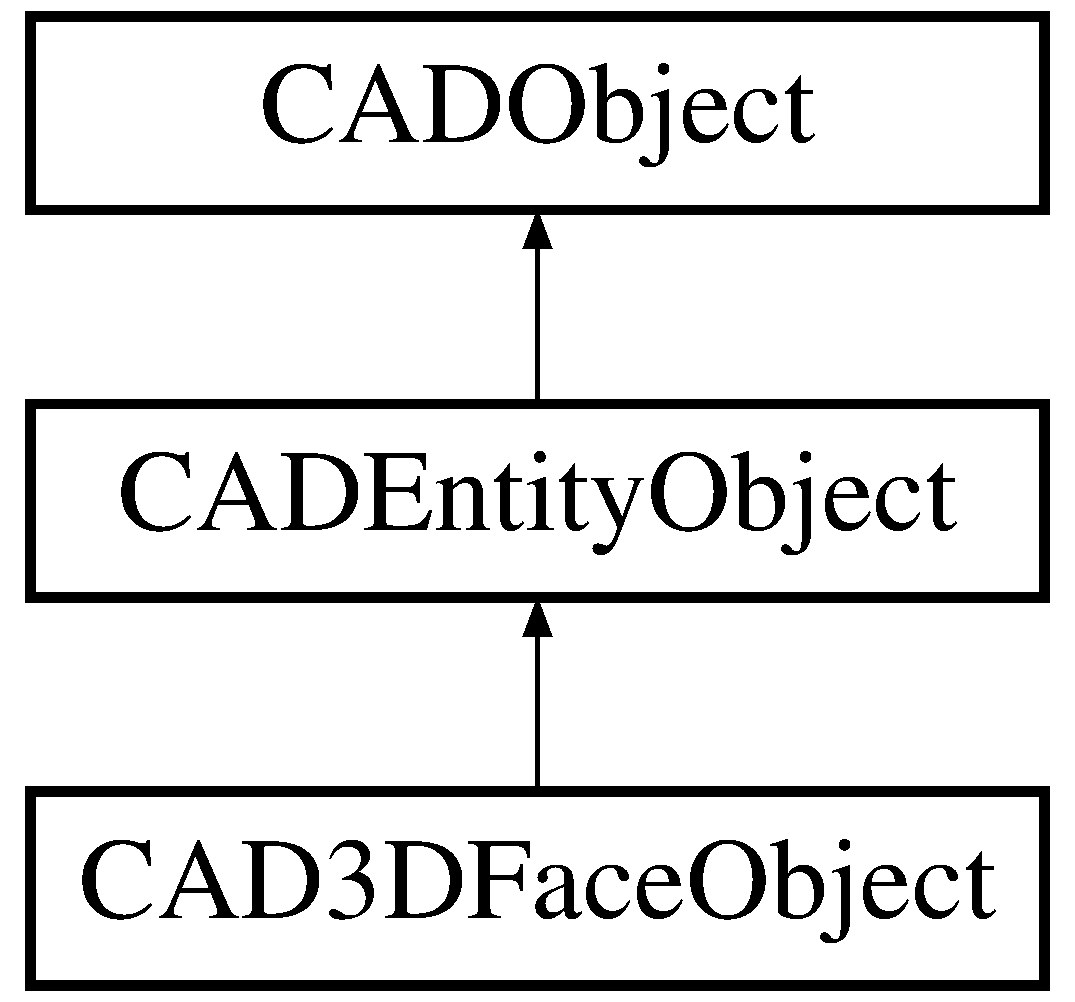
\includegraphics[height=3.000000cm]{class_c_a_d3_d_face_object}
\end{center}
\end{figure}
\subsection*{Public Attributes}
\begin{DoxyCompactItemize}
\item 
bool {\bfseries b\+Has\+No\+Flag\+Ind}\hypertarget{class_c_a_d3_d_face_object_a79dca7ebb3937339dd1161bec6b5cd6b}{}\label{class_c_a_d3_d_face_object_a79dca7ebb3937339dd1161bec6b5cd6b}

\item 
bool {\bfseries b\+Z\+Zero}\hypertarget{class_c_a_d3_d_face_object_ad706e41e727e93ed86942ee5fc1bf191}{}\label{class_c_a_d3_d_face_object_ad706e41e727e93ed86942ee5fc1bf191}

\item 
vector$<$ \hyperlink{class_c_a_d_vector}{C\+A\+D\+Vector} $>$ {\bfseries avert\+Corners}\hypertarget{class_c_a_d3_d_face_object_aeeb82558b3aa77c799f102f5458c865c}{}\label{class_c_a_d3_d_face_object_aeeb82558b3aa77c799f102f5458c865c}

\item 
short {\bfseries d\+Invis\+Flags}\hypertarget{class_c_a_d3_d_face_object_a7b9b1f287c9a57e0cda28d1d3710875c}{}\label{class_c_a_d3_d_face_object_a7b9b1f287c9a57e0cda28d1d3710875c}

\end{DoxyCompactItemize}
\subsection*{Additional Inherited Members}


\subsection{Detailed Description}
The \hyperlink{class_c_a_d3_d_face_object}{C\+A\+D3\+D\+Face\+Object} class. 

The documentation for this class was generated from the following files\+:\begin{DoxyCompactItemize}
\item 
cadobjects.\+h\item 
cadobjects.\+cpp\end{DoxyCompactItemize}

\hypertarget{class_c_a_d_arc}{}\section{C\+A\+D\+Arc Class Reference}
\label{class_c_a_d_arc}\index{C\+A\+D\+Arc@{C\+A\+D\+Arc}}


Geometry class which represents Arc.  




{\ttfamily \#include $<$cadgeometry.\+h$>$}

Inheritance diagram for C\+A\+D\+Arc\+:\begin{figure}[H]
\begin{center}
\leavevmode
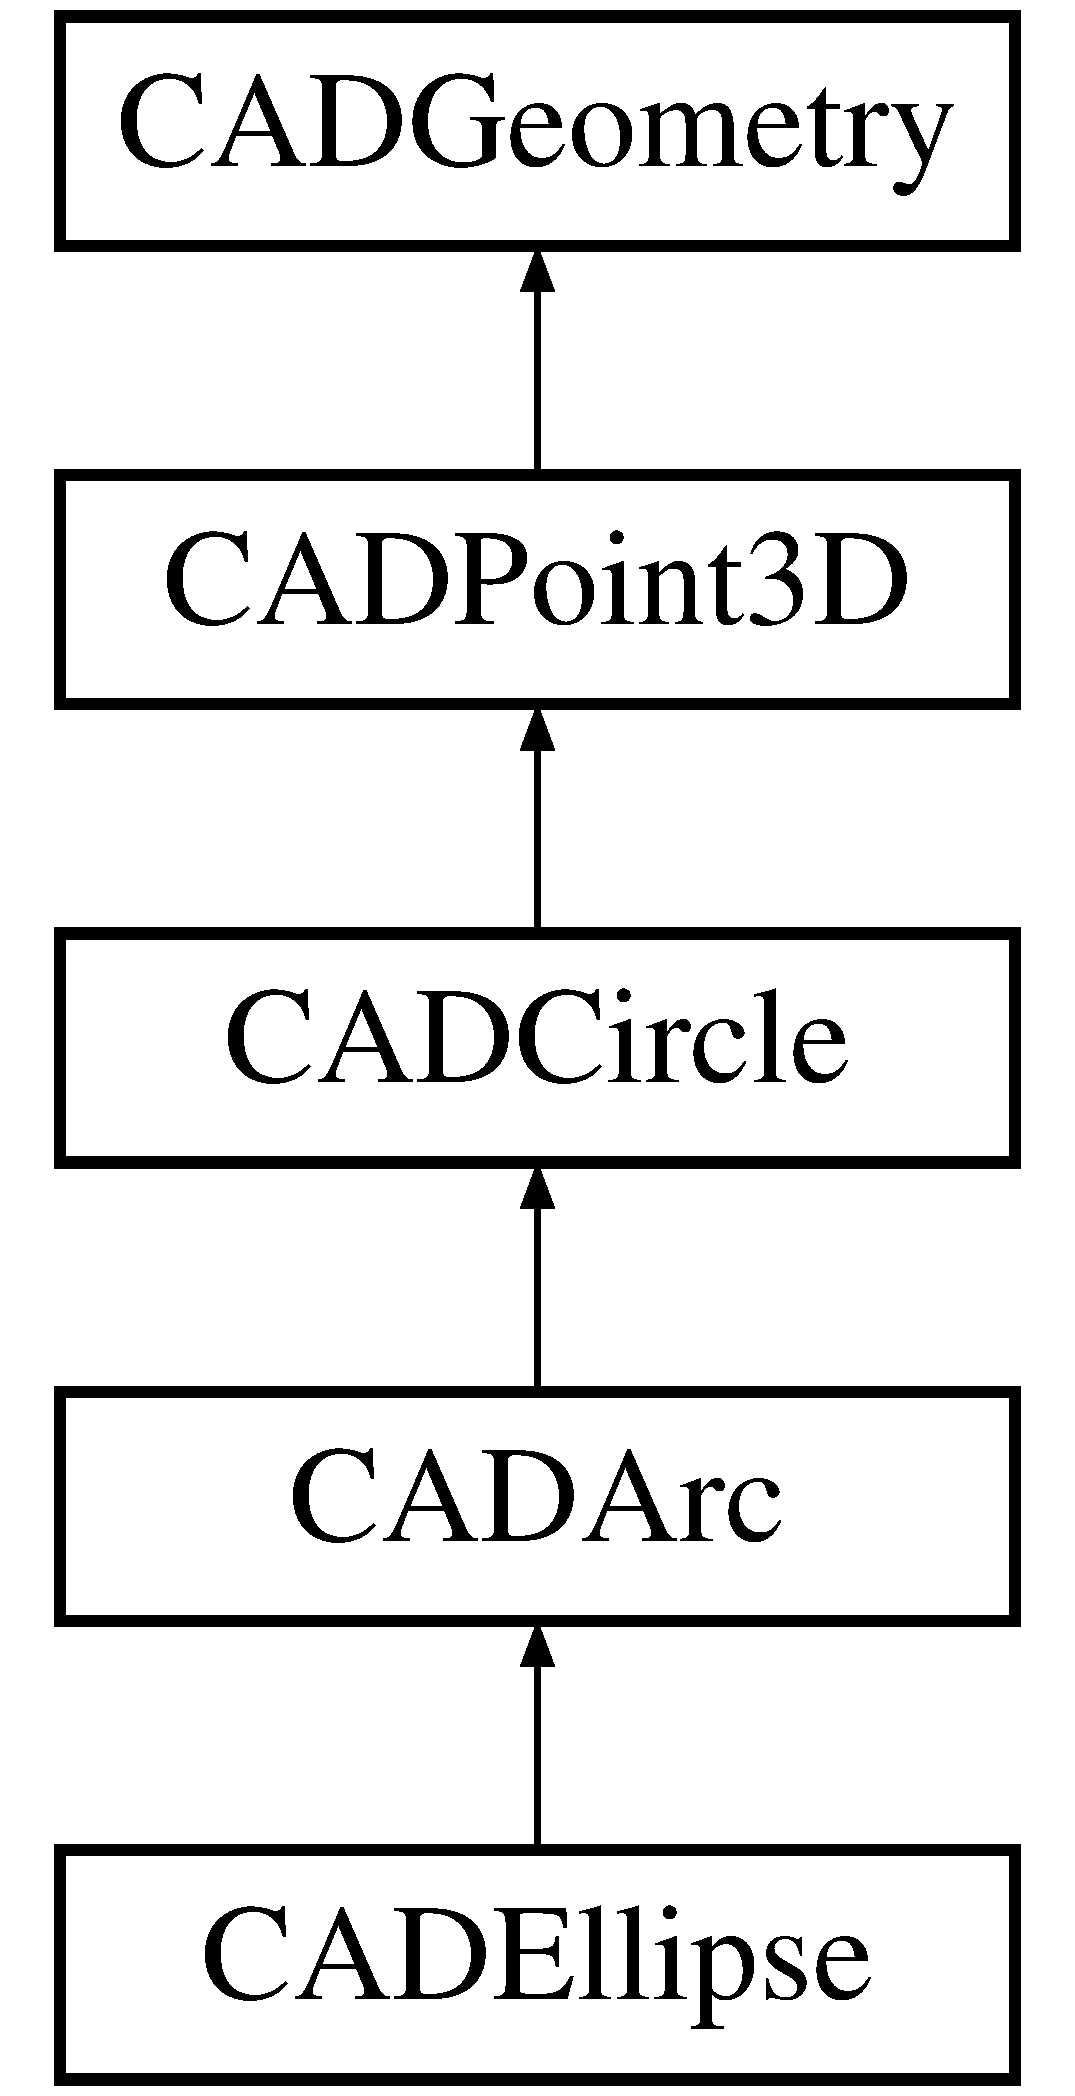
\includegraphics[height=5.000000cm]{class_c_a_d_arc}
\end{center}
\end{figure}
\subsection*{Public Member Functions}
\begin{DoxyCompactItemize}
\item 
double {\bfseries get\+Starting\+Angle} () const \hypertarget{class_c_a_d_arc_a0277ad66f5be5a42657e79c5fc185ffa}{}\label{class_c_a_d_arc_a0277ad66f5be5a42657e79c5fc185ffa}

\item 
void {\bfseries set\+Starting\+Angle} (double value)\hypertarget{class_c_a_d_arc_a5a6c9ca1a413b3c8429a860e05b279e9}{}\label{class_c_a_d_arc_a5a6c9ca1a413b3c8429a860e05b279e9}

\item 
double {\bfseries get\+Ending\+Angle} () const \hypertarget{class_c_a_d_arc_a0e11365230e1aef90a998e0bca6ddc3e}{}\label{class_c_a_d_arc_a0e11365230e1aef90a998e0bca6ddc3e}

\item 
void {\bfseries set\+Ending\+Angle} (double value)\hypertarget{class_c_a_d_arc_abcb9d76ef0df5c1ebe891ca8b38f1576}{}\label{class_c_a_d_arc_abcb9d76ef0df5c1ebe891ca8b38f1576}

\item 
virtual void {\bfseries print} () const  override\hypertarget{class_c_a_d_arc_a0227ac419a5e1412c3daa65bd90f640f}{}\label{class_c_a_d_arc_a0227ac419a5e1412c3daa65bd90f640f}

\end{DoxyCompactItemize}
\subsection*{Protected Attributes}
\begin{DoxyCompactItemize}
\item 
double {\bfseries starting\+Angle}\hypertarget{class_c_a_d_arc_a557edf704b996b0d5f4ea4d6c9dcf7bd}{}\label{class_c_a_d_arc_a557edf704b996b0d5f4ea4d6c9dcf7bd}

\item 
double {\bfseries ending\+Angle}\hypertarget{class_c_a_d_arc_a2f38649ca25a867218afd64596a6c8fe}{}\label{class_c_a_d_arc_a2f38649ca25a867218afd64596a6c8fe}

\end{DoxyCompactItemize}
\subsection*{Additional Inherited Members}


\subsection{Detailed Description}
Geometry class which represents Arc. 

The documentation for this class was generated from the following files\+:\begin{DoxyCompactItemize}
\item 
cadgeometry.\+h\item 
cadgeometry.\+cpp\end{DoxyCompactItemize}

\hypertarget{class_c_a_d_arc_object}{}\section{C\+A\+D\+Arc\+Object Class Reference}
\label{class_c_a_d_arc_object}\index{C\+A\+D\+Arc\+Object@{C\+A\+D\+Arc\+Object}}


The \hyperlink{class_c_a_d_arc}{C\+A\+D\+Arc} class.  




{\ttfamily \#include $<$cadobjects.\+h$>$}

Inheritance diagram for C\+A\+D\+Arc\+Object\+:\begin{figure}[H]
\begin{center}
\leavevmode
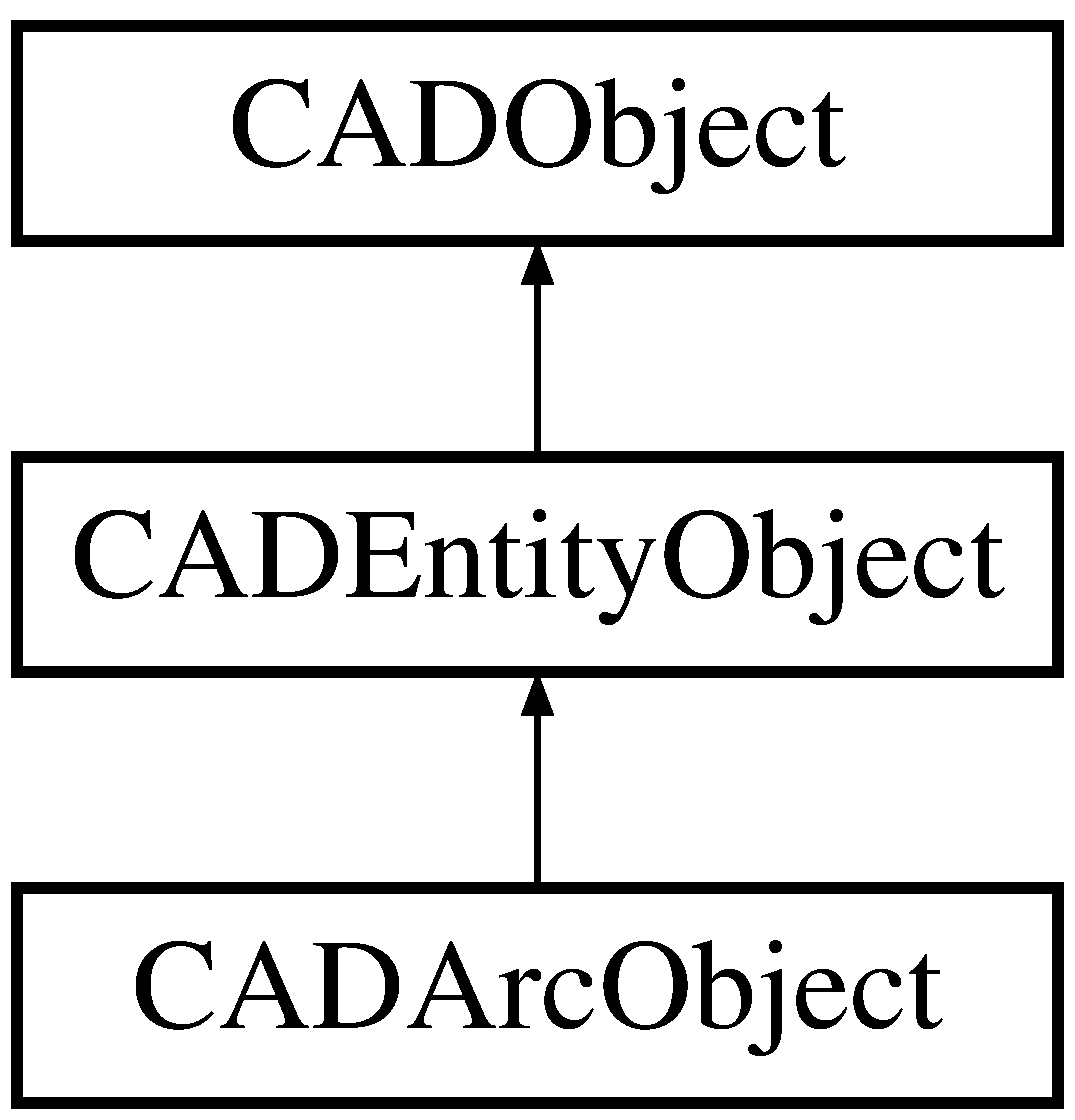
\includegraphics[height=3.000000cm]{class_c_a_d_arc_object}
\end{center}
\end{figure}
\subsection*{Public Attributes}
\begin{DoxyCompactItemize}
\item 
\hyperlink{class_c_a_d_vector}{C\+A\+D\+Vector} {\bfseries vert\+Position}\hypertarget{class_c_a_d_arc_object_ad108019dab2c74864b6e2cbc324f124e}{}\label{class_c_a_d_arc_object_ad108019dab2c74864b6e2cbc324f124e}

\item 
double {\bfseries df\+Radius}\hypertarget{class_c_a_d_arc_object_ae4d725a232be0bab918c3d5a42c62850}{}\label{class_c_a_d_arc_object_ae4d725a232be0bab918c3d5a42c62850}

\item 
double {\bfseries df\+Thickness}\hypertarget{class_c_a_d_arc_object_aab0ddf06e36b1076479e10b67ea6318b}{}\label{class_c_a_d_arc_object_aab0ddf06e36b1076479e10b67ea6318b}

\item 
\hyperlink{class_c_a_d_vector}{C\+A\+D\+Vector} {\bfseries vect\+Extrusion}\hypertarget{class_c_a_d_arc_object_a6ca29b696f21ffcbec73c1ccb76af871}{}\label{class_c_a_d_arc_object_a6ca29b696f21ffcbec73c1ccb76af871}

\item 
double {\bfseries df\+Start\+Angle}\hypertarget{class_c_a_d_arc_object_a8d1dd7e43a8af7fd0be782ec0ca25218}{}\label{class_c_a_d_arc_object_a8d1dd7e43a8af7fd0be782ec0ca25218}

\item 
double {\bfseries df\+End\+Angle}\hypertarget{class_c_a_d_arc_object_a908abe29d8cb4cc2cfdfcacc42d8a896}{}\label{class_c_a_d_arc_object_a908abe29d8cb4cc2cfdfcacc42d8a896}

\end{DoxyCompactItemize}
\subsection*{Additional Inherited Members}


\subsection{Detailed Description}
The \hyperlink{class_c_a_d_arc}{C\+A\+D\+Arc} class. 

The documentation for this class was generated from the following files\+:\begin{DoxyCompactItemize}
\item 
cadobjects.\+h\item 
cadobjects.\+cpp\end{DoxyCompactItemize}

\hypertarget{class_c_a_d_attdef}{}\section{C\+A\+D\+Attdef Class Reference}
\label{class_c_a_d_attdef}\index{C\+A\+D\+Attdef@{C\+A\+D\+Attdef}}


Geometry class which represents Attribute definition.  




{\ttfamily \#include $<$cadgeometry.\+h$>$}

Inheritance diagram for C\+A\+D\+Attdef\+:\begin{figure}[H]
\begin{center}
\leavevmode
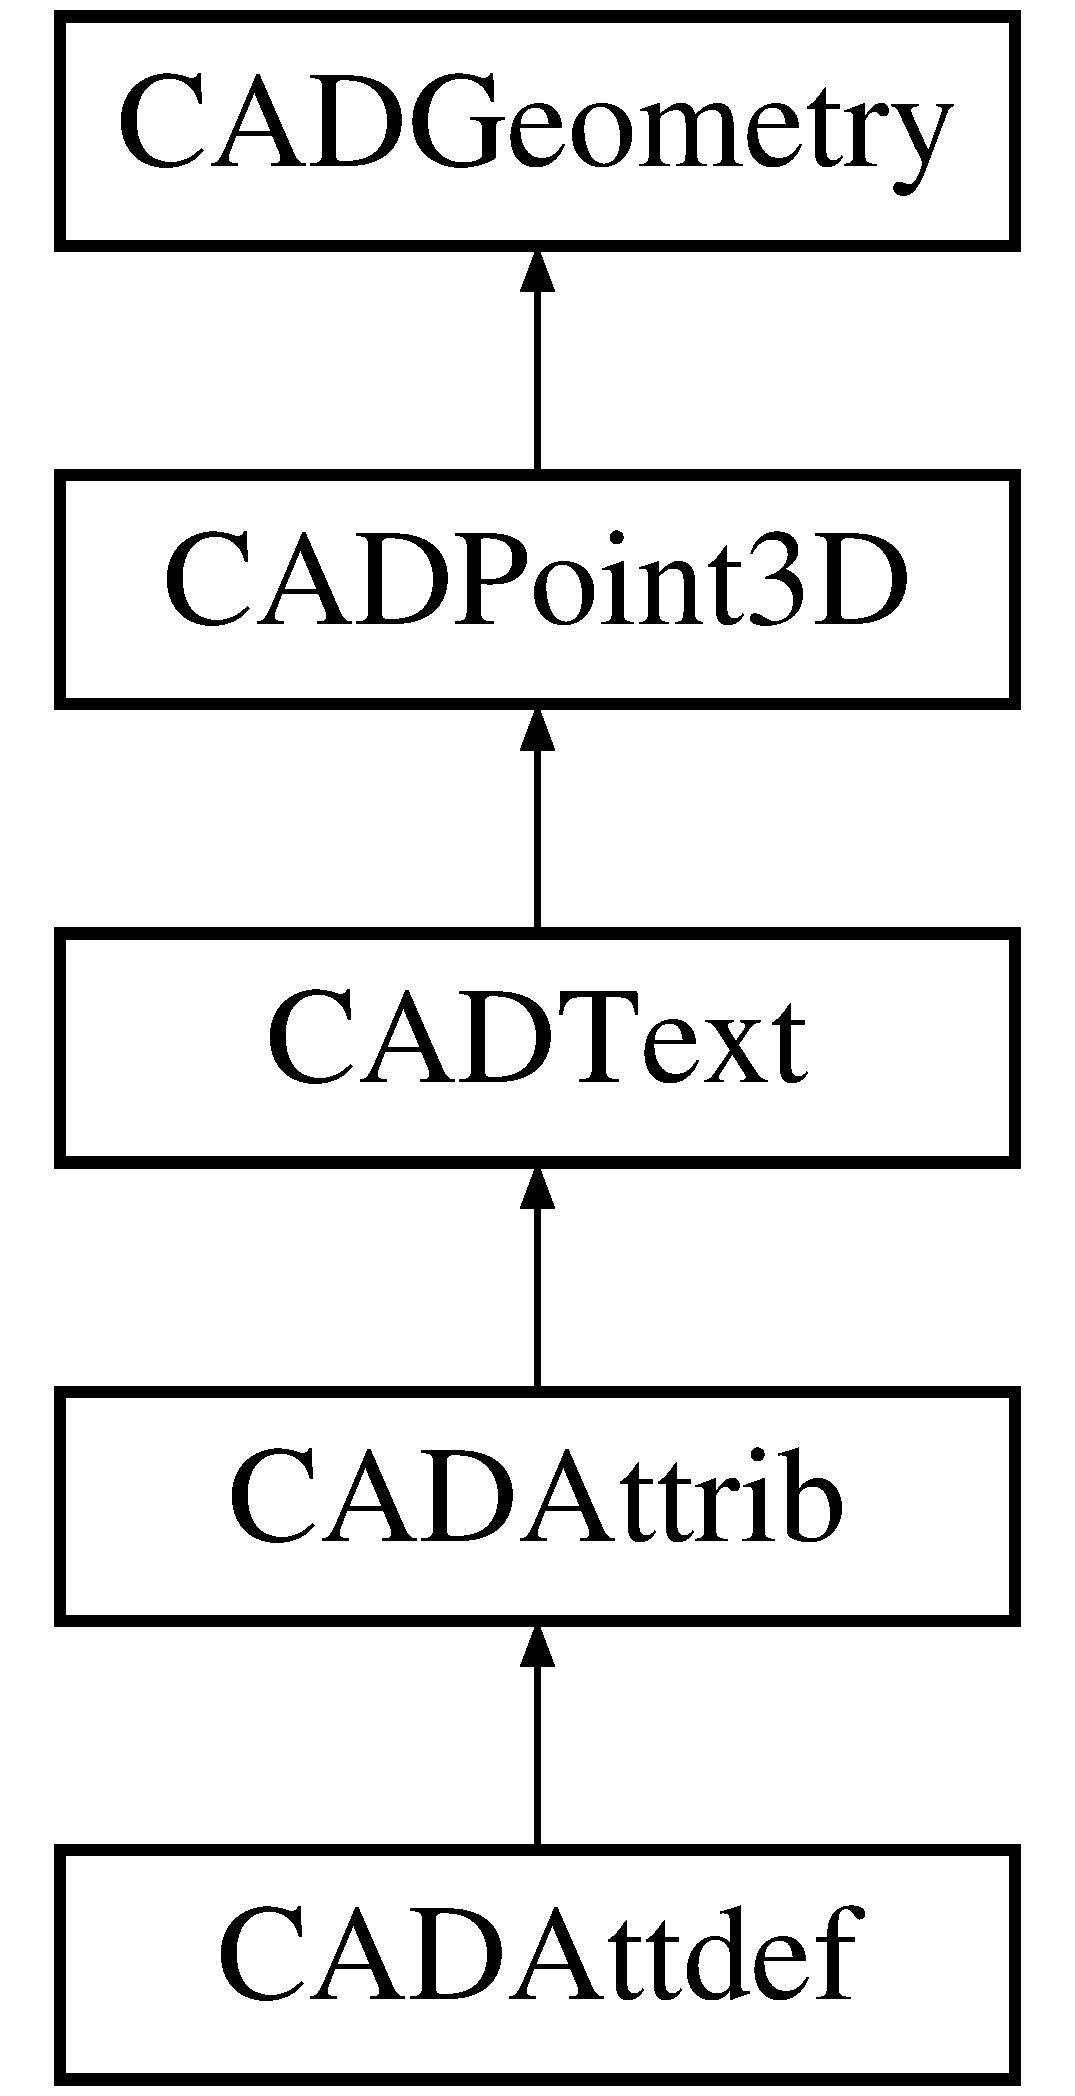
\includegraphics[height=5.000000cm]{class_c_a_d_attdef}
\end{center}
\end{figure}
\subsection*{Public Member Functions}
\begin{DoxyCompactItemize}
\item 
virtual void {\bfseries print} () const  override\hypertarget{class_c_a_d_attdef_afda633f92e0cf0cbbc30fe7cdb21457e}{}\label{class_c_a_d_attdef_afda633f92e0cf0cbbc30fe7cdb21457e}

\item 
string {\bfseries get\+Prompt} () const \hypertarget{class_c_a_d_attdef_ac862ce2b130777db87b861f7bf80e530}{}\label{class_c_a_d_attdef_ac862ce2b130777db87b861f7bf80e530}

\item 
void {\bfseries set\+Prompt} (const string \&)\hypertarget{class_c_a_d_attdef_ab8597b99e32dcb8b4e9c9436ee104219}{}\label{class_c_a_d_attdef_ab8597b99e32dcb8b4e9c9436ee104219}

\end{DoxyCompactItemize}
\subsection*{Protected Attributes}
\begin{DoxyCompactItemize}
\item 
string {\bfseries s\+Prompt}\hypertarget{class_c_a_d_attdef_aceae65be743858330a8b8d765935d16b}{}\label{class_c_a_d_attdef_aceae65be743858330a8b8d765935d16b}

\end{DoxyCompactItemize}
\subsection*{Additional Inherited Members}


\subsection{Detailed Description}
Geometry class which represents Attribute definition. 

The documentation for this class was generated from the following files\+:\begin{DoxyCompactItemize}
\item 
cadgeometry.\+h\item 
cadgeometry.\+cpp\end{DoxyCompactItemize}

\hypertarget{class_c_a_d_attdef_object}{}\section{C\+A\+D\+Attdef\+Object Class Reference}
\label{class_c_a_d_attdef_object}\index{C\+A\+D\+Attdef\+Object@{C\+A\+D\+Attdef\+Object}}


The C\+AD Attribute definition Object class.  




{\ttfamily \#include $<$cadobjects.\+h$>$}

Inheritance diagram for C\+A\+D\+Attdef\+Object\+:\begin{figure}[H]
\begin{center}
\leavevmode
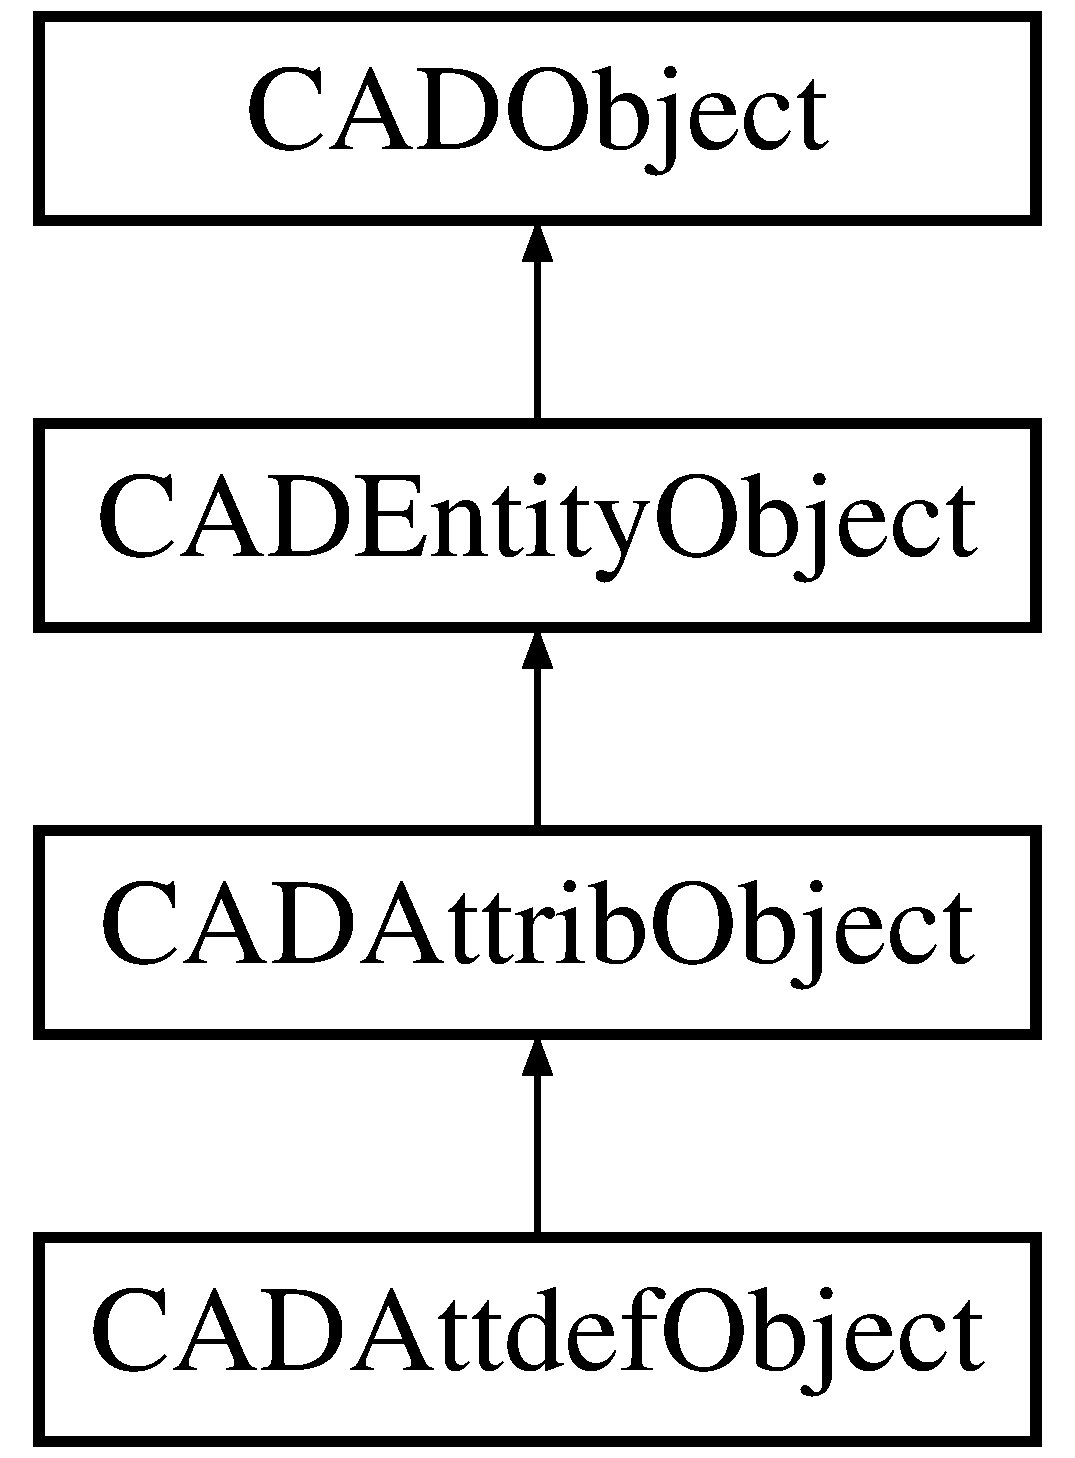
\includegraphics[height=4.000000cm]{class_c_a_d_attdef_object}
\end{center}
\end{figure}
\subsection*{Public Attributes}
\begin{DoxyCompactItemize}
\item 
string {\bfseries s\+Prompt}\hypertarget{class_c_a_d_attdef_object_a740ca29cffee8eda821d174b3174f6c1}{}\label{class_c_a_d_attdef_object_a740ca29cffee8eda821d174b3174f6c1}

\end{DoxyCompactItemize}
\subsection*{Additional Inherited Members}


\subsection{Detailed Description}
The C\+AD Attribute definition Object class. 

The documentation for this class was generated from the following files\+:\begin{DoxyCompactItemize}
\item 
cadobjects.\+h\item 
cadobjects.\+cpp\end{DoxyCompactItemize}

\hypertarget{class_c_a_d_attrib}{}\section{C\+A\+D\+Attrib Class Reference}
\label{class_c_a_d_attrib}\index{C\+A\+D\+Attrib@{C\+A\+D\+Attrib}}


Geometry class which represents Attribute.  




{\ttfamily \#include $<$cadgeometry.\+h$>$}

Inheritance diagram for C\+A\+D\+Attrib\+:\begin{figure}[H]
\begin{center}
\leavevmode
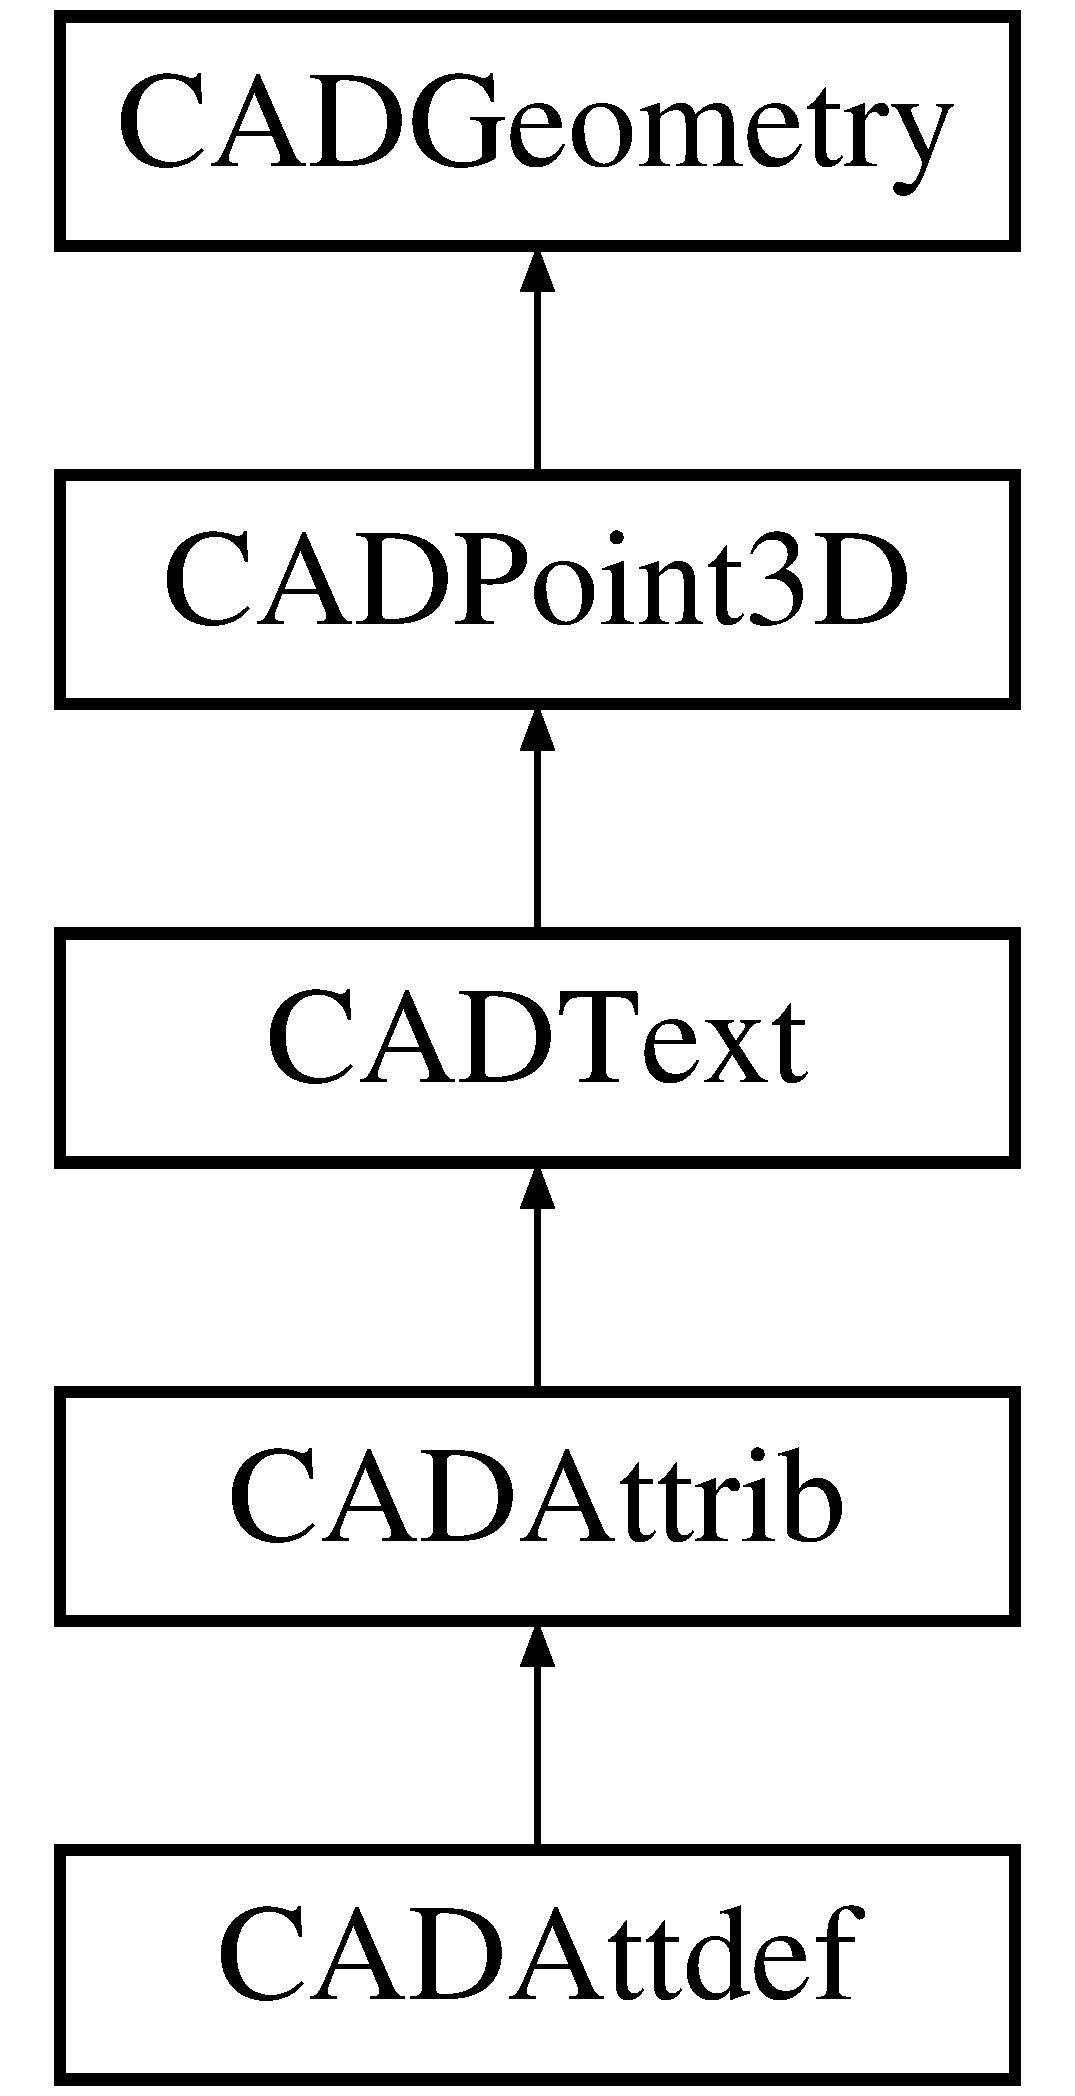
\includegraphics[height=5.000000cm]{class_c_a_d_attrib}
\end{center}
\end{figure}
\subsection*{Public Member Functions}
\begin{DoxyCompactItemize}
\item 
virtual void {\bfseries print} () const  override\hypertarget{class_c_a_d_attrib_a78cb6805de2667a8e72f3906d84a58b6}{}\label{class_c_a_d_attrib_a78cb6805de2667a8e72f3906d84a58b6}

\item 
double {\bfseries get\+Elevation} () const \hypertarget{class_c_a_d_attrib_afb3c3335f16852f401d7313fcb9dc637}{}\label{class_c_a_d_attrib_afb3c3335f16852f401d7313fcb9dc637}

\item 
void {\bfseries set\+Elevation} (double)\hypertarget{class_c_a_d_attrib_aff3d2d57609b1bbd98d393dc55498da5}{}\label{class_c_a_d_attrib_aff3d2d57609b1bbd98d393dc55498da5}

\item 
string {\bfseries get\+Tag} () const \hypertarget{class_c_a_d_attrib_a197eaef21150a38ffc4a0011195329f7}{}\label{class_c_a_d_attrib_a197eaef21150a38ffc4a0011195329f7}

\item 
void {\bfseries set\+Tag} (const string \&)\hypertarget{class_c_a_d_attrib_a51dbe97cbccb9228e35e5e5a0d321bbb}{}\label{class_c_a_d_attrib_a51dbe97cbccb9228e35e5e5a0d321bbb}

\item 
\hyperlink{class_c_a_d_vector}{C\+A\+D\+Vector} {\bfseries get\+Alignment\+Point} () const \hypertarget{class_c_a_d_attrib_a3885ec44a8b70a2bc2a55048f9f36aac}{}\label{class_c_a_d_attrib_a3885ec44a8b70a2bc2a55048f9f36aac}

\item 
void {\bfseries set\+Alignment\+Point} (const \hyperlink{class_c_a_d_vector}{C\+A\+D\+Vector} \&)\hypertarget{class_c_a_d_attrib_a81b06be0005dcbc51ce95378785dbc44}{}\label{class_c_a_d_attrib_a81b06be0005dcbc51ce95378785dbc44}

\item 
bool {\bfseries is\+Position\+Locked} () const \hypertarget{class_c_a_d_attrib_aacb0f9874e95a0e4d4e24afa86e25cee}{}\label{class_c_a_d_attrib_aacb0f9874e95a0e4d4e24afa86e25cee}

\item 
void {\bfseries set\+Position\+Locked} (bool)\hypertarget{class_c_a_d_attrib_aa4e342b54aeb90cded953f8e47f32b08}{}\label{class_c_a_d_attrib_aa4e342b54aeb90cded953f8e47f32b08}

\end{DoxyCompactItemize}
\subsection*{Protected Attributes}
\begin{DoxyCompactItemize}
\item 
\hyperlink{class_c_a_d_vector}{C\+A\+D\+Vector} {\bfseries vert\+Alignment\+Point}\hypertarget{class_c_a_d_attrib_aead893b2d8dcb83afd25b379a2d18185}{}\label{class_c_a_d_attrib_aead893b2d8dcb83afd25b379a2d18185}

\item 
double {\bfseries df\+Elevation}\hypertarget{class_c_a_d_attrib_a7aec72015ed67dec7bd81e9400af1a32}{}\label{class_c_a_d_attrib_a7aec72015ed67dec7bd81e9400af1a32}

\item 
string {\bfseries s\+Tag}\hypertarget{class_c_a_d_attrib_a739fe51000f950dac526f397eaa995aa}{}\label{class_c_a_d_attrib_a739fe51000f950dac526f397eaa995aa}

\item 
bool {\bfseries b\+Lock\+Position}\hypertarget{class_c_a_d_attrib_ac57f77ae05f7651e4c9266796d4e335a}{}\label{class_c_a_d_attrib_ac57f77ae05f7651e4c9266796d4e335a}

\end{DoxyCompactItemize}
\subsection*{Additional Inherited Members}


\subsection{Detailed Description}
Geometry class which represents Attribute. 

The documentation for this class was generated from the following files\+:\begin{DoxyCompactItemize}
\item 
cadgeometry.\+h\item 
cadgeometry.\+cpp\end{DoxyCompactItemize}

\hypertarget{class_c_a_d_attrib_object}{}\section{C\+A\+D\+Attrib\+Object Class Reference}
\label{class_c_a_d_attrib_object}\index{C\+A\+D\+Attrib\+Object@{C\+A\+D\+Attrib\+Object}}


The C\+AD Attribute Object class.  




{\ttfamily \#include $<$cadobjects.\+h$>$}

Inheritance diagram for C\+A\+D\+Attrib\+Object\+:\begin{figure}[H]
\begin{center}
\leavevmode
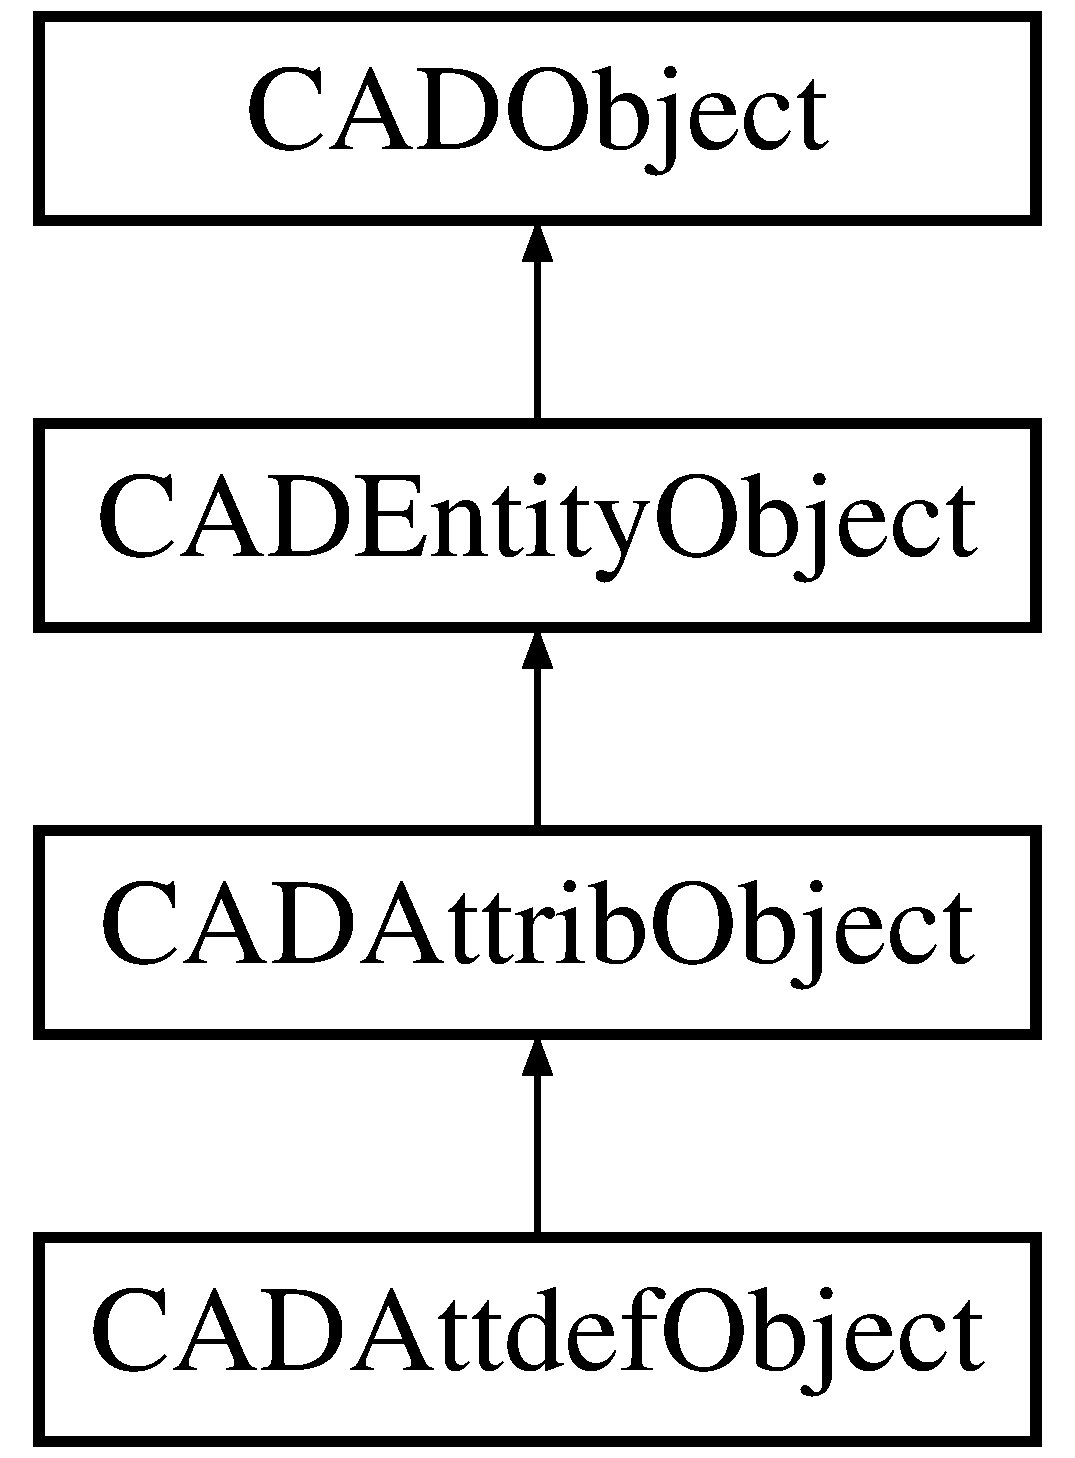
\includegraphics[height=4.000000cm]{class_c_a_d_attrib_object}
\end{center}
\end{figure}
\subsection*{Public Attributes}
\begin{DoxyCompactItemize}
\item 
unsigned char {\bfseries Data\+Flags}\hypertarget{class_c_a_d_attrib_object_a88c325df5421e4db2de66f4cf0971e72}{}\label{class_c_a_d_attrib_object_a88c325df5421e4db2de66f4cf0971e72}

\item 
double {\bfseries df\+Elevation}\hypertarget{class_c_a_d_attrib_object_a1ee811d7ad728989510657e891985dbb}{}\label{class_c_a_d_attrib_object_a1ee811d7ad728989510657e891985dbb}

\item 
\hyperlink{class_c_a_d_vector}{C\+A\+D\+Vector} {\bfseries vert\+Insetion\+Point}\hypertarget{class_c_a_d_attrib_object_a4c575c87c3a89db38a6b3e7c84a1d661}{}\label{class_c_a_d_attrib_object_a4c575c87c3a89db38a6b3e7c84a1d661}

\item 
\hyperlink{class_c_a_d_vector}{C\+A\+D\+Vector} {\bfseries vert\+Alignment\+Point}\hypertarget{class_c_a_d_attrib_object_ae2b507f8e45ce015d8e8dc0bed8e2487}{}\label{class_c_a_d_attrib_object_ae2b507f8e45ce015d8e8dc0bed8e2487}

\item 
\hyperlink{class_c_a_d_vector}{C\+A\+D\+Vector} {\bfseries vect\+Extrusion}\hypertarget{class_c_a_d_attrib_object_a83cfae162fc79ba9731db8a25928d4a8}{}\label{class_c_a_d_attrib_object_a83cfae162fc79ba9731db8a25928d4a8}

\item 
double {\bfseries df\+Thickness}\hypertarget{class_c_a_d_attrib_object_afd4a4e33fad64b372a5d2103863b0d52}{}\label{class_c_a_d_attrib_object_afd4a4e33fad64b372a5d2103863b0d52}

\item 
double {\bfseries df\+Oblique\+Ang}\hypertarget{class_c_a_d_attrib_object_acefcb68acacc73bb50cec6c4c426e4fe}{}\label{class_c_a_d_attrib_object_acefcb68acacc73bb50cec6c4c426e4fe}

\item 
double {\bfseries df\+Rotation\+Ang}\hypertarget{class_c_a_d_attrib_object_ae8570270f149555714d597193f284aed}{}\label{class_c_a_d_attrib_object_ae8570270f149555714d597193f284aed}

\item 
double {\bfseries df\+Height}\hypertarget{class_c_a_d_attrib_object_a31798e8c252f99c111cc66f216c2ab9a}{}\label{class_c_a_d_attrib_object_a31798e8c252f99c111cc66f216c2ab9a}

\item 
double {\bfseries df\+Width\+Factor}\hypertarget{class_c_a_d_attrib_object_aaec92dc411d415cba032015350cdf4a5}{}\label{class_c_a_d_attrib_object_aaec92dc411d415cba032015350cdf4a5}

\item 
string {\bfseries s\+Text\+Value}\hypertarget{class_c_a_d_attrib_object_ac02b8fa34067fd22e5ef75ce21492357}{}\label{class_c_a_d_attrib_object_ac02b8fa34067fd22e5ef75ce21492357}

\item 
short {\bfseries d\+Generation}\hypertarget{class_c_a_d_attrib_object_a954802bd7cac362caf8697ab48c7f327}{}\label{class_c_a_d_attrib_object_a954802bd7cac362caf8697ab48c7f327}

\item 
short {\bfseries d\+Horiz\+Align}\hypertarget{class_c_a_d_attrib_object_a949ff12666b3ea425f9098c145052c3a}{}\label{class_c_a_d_attrib_object_a949ff12666b3ea425f9098c145052c3a}

\item 
short {\bfseries d\+Vert\+Align}\hypertarget{class_c_a_d_attrib_object_a620af63d2fb8a4a9b1dc725def15e2ce}{}\label{class_c_a_d_attrib_object_a620af63d2fb8a4a9b1dc725def15e2ce}

\item 
char {\bfseries d\+Version}\hypertarget{class_c_a_d_attrib_object_a67242adb97cea205ad5f0d43cb38b2b6}{}\label{class_c_a_d_attrib_object_a67242adb97cea205ad5f0d43cb38b2b6}

\item 
string {\bfseries s\+Tag}\hypertarget{class_c_a_d_attrib_object_a716414edefc4773fdebf79635db634ab}{}\label{class_c_a_d_attrib_object_a716414edefc4773fdebf79635db634ab}

\item 
short {\bfseries n\+Field\+Length}\hypertarget{class_c_a_d_attrib_object_ac40341768856cca5e4a08f81a4af6953}{}\label{class_c_a_d_attrib_object_ac40341768856cca5e4a08f81a4af6953}

\item 
unsigned char {\bfseries n\+Flags}\hypertarget{class_c_a_d_attrib_object_a761d21c1b2c1a9aa52083459be267a35}{}\label{class_c_a_d_attrib_object_a761d21c1b2c1a9aa52083459be267a35}

\item 
bool {\bfseries b\+Lock\+Position}\hypertarget{class_c_a_d_attrib_object_af48070a4673e9332672c4d476e0d24e0}{}\label{class_c_a_d_attrib_object_af48070a4673e9332672c4d476e0d24e0}

\item 
\hyperlink{class_c_a_d_handle}{C\+A\+D\+Handle} {\bfseries h\+Style}\hypertarget{class_c_a_d_attrib_object_a225481dff5317a3d2dcb676d801f1fe1}{}\label{class_c_a_d_attrib_object_a225481dff5317a3d2dcb676d801f1fe1}

\end{DoxyCompactItemize}
\subsection*{Additional Inherited Members}


\subsection{Detailed Description}
The C\+AD Attribute Object class. 

The documentation for this class was generated from the following files\+:\begin{DoxyCompactItemize}
\item 
cadobjects.\+h\item 
cadobjects.\+cpp\end{DoxyCompactItemize}

\hypertarget{class_c_a_d_block_control_object}{}\section{C\+A\+D\+Block\+Control\+Object Class Reference}
\label{class_c_a_d_block_control_object}\index{C\+A\+D\+Block\+Control\+Object@{C\+A\+D\+Block\+Control\+Object}}


The \hyperlink{class_c_a_d_block_control_object}{C\+A\+D\+Block\+Control\+Object} class.  




{\ttfamily \#include $<$cadobjects.\+h$>$}

Inheritance diagram for C\+A\+D\+Block\+Control\+Object\+:\begin{figure}[H]
\begin{center}
\leavevmode
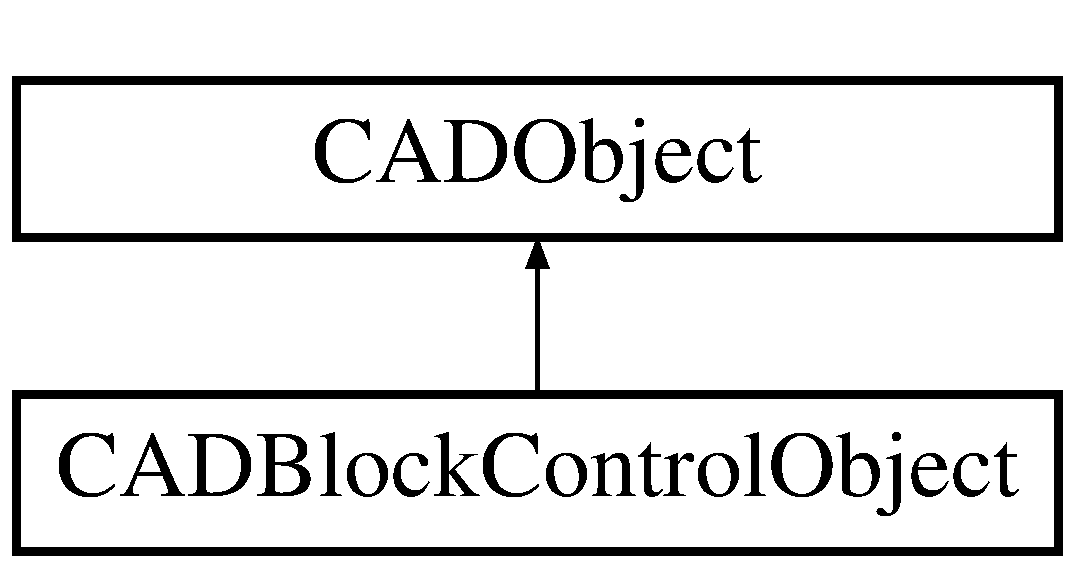
\includegraphics[height=2.000000cm]{class_c_a_d_block_control_object}
\end{center}
\end{figure}
\subsection*{Public Attributes}
\begin{DoxyCompactItemize}
\item 
long {\bfseries n\+Object\+Size\+In\+Bits}\hypertarget{class_c_a_d_block_control_object_adfd5c1ecaa8f2aedd307a508e4aada5c}{}\label{class_c_a_d_block_control_object_adfd5c1ecaa8f2aedd307a508e4aada5c}

\item 
\hyperlink{class_c_a_d_handle}{C\+A\+D\+Handle} {\bfseries h\+Object\+Handle}\hypertarget{class_c_a_d_block_control_object_a5a715c5543e9c768deb85a758348b25a}{}\label{class_c_a_d_block_control_object_a5a715c5543e9c768deb85a758348b25a}

\item 
C\+A\+D\+Eed\+Array {\bfseries a\+E\+ED}\hypertarget{class_c_a_d_block_control_object_a0c1229f562b5a548da6ff1b51ccbc211}{}\label{class_c_a_d_block_control_object_a0c1229f562b5a548da6ff1b51ccbc211}

\item 
long {\bfseries n\+Num\+Reactors}\hypertarget{class_c_a_d_block_control_object_a17a32ac995a391809b836fff9d21771c}{}\label{class_c_a_d_block_control_object_a17a32ac995a391809b836fff9d21771c}

\item 
bool {\bfseries b\+No\+X\+Dictionary\+Present}\hypertarget{class_c_a_d_block_control_object_a8d57585b345f9b703c93191563bfaa49}{}\label{class_c_a_d_block_control_object_a8d57585b345f9b703c93191563bfaa49}

\item 
long {\bfseries n\+Num\+Entries}\hypertarget{class_c_a_d_block_control_object_a7213b7bac1fb7725c722bf53304f3e7b}{}\label{class_c_a_d_block_control_object_a7213b7bac1fb7725c722bf53304f3e7b}

\item 
\hyperlink{class_c_a_d_handle}{C\+A\+D\+Handle} {\bfseries h\+Null}\hypertarget{class_c_a_d_block_control_object_ae0ea6b61178a4742fc721815ec93f2c9}{}\label{class_c_a_d_block_control_object_ae0ea6b61178a4742fc721815ec93f2c9}

\item 
\hyperlink{class_c_a_d_handle}{C\+A\+D\+Handle} {\bfseries h\+X\+Dictionary}\hypertarget{class_c_a_d_block_control_object_a4f7992998912d33967fe411feb404fcf}{}\label{class_c_a_d_block_control_object_a4f7992998912d33967fe411feb404fcf}

\item 
C\+A\+D\+Handle\+Array {\bfseries h\+Blocks}\hypertarget{class_c_a_d_block_control_object_ac06b2e7d6754e7039060c07b7913c998}{}\label{class_c_a_d_block_control_object_ac06b2e7d6754e7039060c07b7913c998}

\end{DoxyCompactItemize}
\subsection*{Additional Inherited Members}


\subsection{Detailed Description}
The \hyperlink{class_c_a_d_block_control_object}{C\+A\+D\+Block\+Control\+Object} class. 

The documentation for this class was generated from the following files\+:\begin{DoxyCompactItemize}
\item 
cadobjects.\+h\item 
cadobjects.\+cpp\end{DoxyCompactItemize}

\hypertarget{class_c_a_d_block_header_object}{}\section{C\+A\+D\+Block\+Header\+Object Class Reference}
\label{class_c_a_d_block_header_object}\index{C\+A\+D\+Block\+Header\+Object@{C\+A\+D\+Block\+Header\+Object}}


The \hyperlink{class_c_a_d_block_header_object}{C\+A\+D\+Block\+Header\+Object} class.  




{\ttfamily \#include $<$cadobjects.\+h$>$}

Inheritance diagram for C\+A\+D\+Block\+Header\+Object\+:\begin{figure}[H]
\begin{center}
\leavevmode
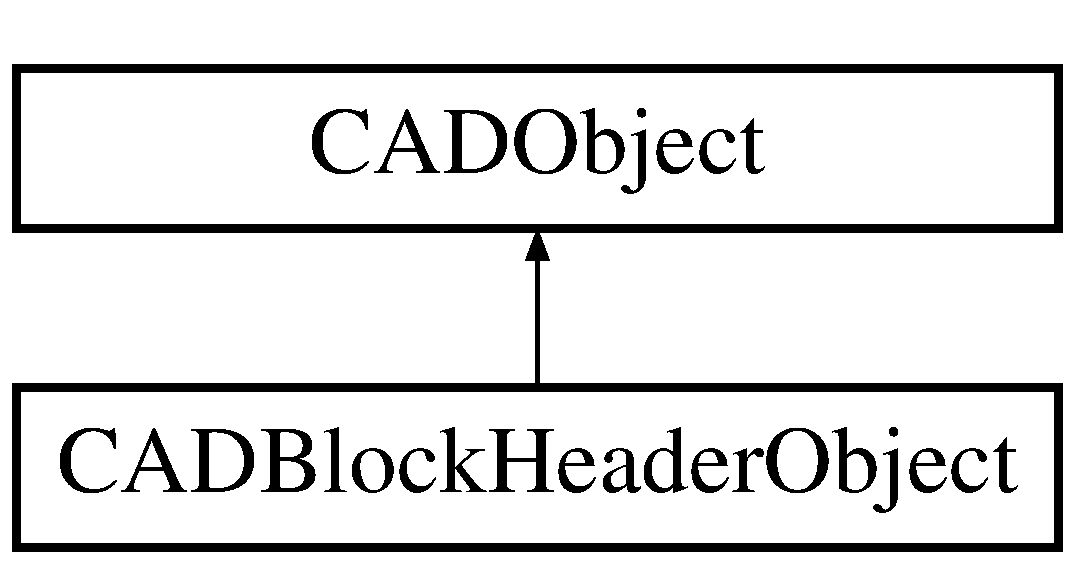
\includegraphics[height=2.000000cm]{class_c_a_d_block_header_object}
\end{center}
\end{figure}
\subsection*{Public Attributes}
\begin{DoxyCompactItemize}
\item 
long {\bfseries n\+Object\+Size\+In\+Bits}\hypertarget{class_c_a_d_block_header_object_aa346bd1a9b20a31721a368e8f70c0e3d}{}\label{class_c_a_d_block_header_object_aa346bd1a9b20a31721a368e8f70c0e3d}

\item 
\hyperlink{class_c_a_d_handle}{C\+A\+D\+Handle} {\bfseries h\+Object\+Handle}\hypertarget{class_c_a_d_block_header_object_a5478612aa01ae3cf1e7208ba3c838d73}{}\label{class_c_a_d_block_header_object_a5478612aa01ae3cf1e7208ba3c838d73}

\item 
C\+A\+D\+Eed\+Array {\bfseries a\+E\+ED}\hypertarget{class_c_a_d_block_header_object_a6173e727adc4fffecf98125b7f103b2a}{}\label{class_c_a_d_block_header_object_a6173e727adc4fffecf98125b7f103b2a}

\item 
long {\bfseries n\+Num\+Reactors}\hypertarget{class_c_a_d_block_header_object_aec8466b6ca1922bece2e3c3cdf8cee89}{}\label{class_c_a_d_block_header_object_aec8466b6ca1922bece2e3c3cdf8cee89}

\item 
bool {\bfseries b\+No\+X\+Dictionary\+Present}\hypertarget{class_c_a_d_block_header_object_a5c6121e7ff9bdc40f066805ac77debb4}{}\label{class_c_a_d_block_header_object_a5c6121e7ff9bdc40f066805ac77debb4}

\item 
string {\bfseries s\+Entry\+Name}\hypertarget{class_c_a_d_block_header_object_ab52ff1b067ae9fb80767dd3fb8a7cc13}{}\label{class_c_a_d_block_header_object_ab52ff1b067ae9fb80767dd3fb8a7cc13}

\item 
bool {\bfseries b64\+Flag}\hypertarget{class_c_a_d_block_header_object_a8a3fdb0f4b807086f5e618bc6ce1e774}{}\label{class_c_a_d_block_header_object_a8a3fdb0f4b807086f5e618bc6ce1e774}

\item 
short {\bfseries d\+X\+Ref\+Index}\hypertarget{class_c_a_d_block_header_object_ac722cb2fb401fc73a1ddd64f146cf187}{}\label{class_c_a_d_block_header_object_ac722cb2fb401fc73a1ddd64f146cf187}

\item 
bool {\bfseries b\+X\+Dep}\hypertarget{class_c_a_d_block_header_object_a8a3c1c97404a2cf868a2f8ce08c5cd3a}{}\label{class_c_a_d_block_header_object_a8a3c1c97404a2cf868a2f8ce08c5cd3a}

\item 
bool {\bfseries b\+Anonymous}\hypertarget{class_c_a_d_block_header_object_a44026fd9f936b6712a876d1d145bb77b}{}\label{class_c_a_d_block_header_object_a44026fd9f936b6712a876d1d145bb77b}

\item 
bool {\bfseries b\+Has\+Atts}\hypertarget{class_c_a_d_block_header_object_a2308c4f43e3f366747e0431a943f8f4a}{}\label{class_c_a_d_block_header_object_a2308c4f43e3f366747e0431a943f8f4a}

\item 
bool {\bfseries b\+Blkis\+X\+Ref}\hypertarget{class_c_a_d_block_header_object_a8bc08e137741912a2289666ccabaa252}{}\label{class_c_a_d_block_header_object_a8bc08e137741912a2289666ccabaa252}

\item 
bool {\bfseries b\+X\+Ref\+Overlaid}\hypertarget{class_c_a_d_block_header_object_a4d913cfa1db80dde6cc5e486e09038c2}{}\label{class_c_a_d_block_header_object_a4d913cfa1db80dde6cc5e486e09038c2}

\item 
bool {\bfseries b\+Loaded\+Bit}\hypertarget{class_c_a_d_block_header_object_a71213627479307625d7f3a98a2c18da3}{}\label{class_c_a_d_block_header_object_a71213627479307625d7f3a98a2c18da3}

\item 
long {\bfseries n\+Owned\+Objects\+Count}\hypertarget{class_c_a_d_block_header_object_ae5a80745ee95dd4271f9cc4d36e3377f}{}\label{class_c_a_d_block_header_object_ae5a80745ee95dd4271f9cc4d36e3377f}

\item 
\hyperlink{class_c_a_d_vector}{C\+A\+D\+Vector} {\bfseries vert\+Base\+Point}\hypertarget{class_c_a_d_block_header_object_a0237262a510d9de7f962e829d17f60b2}{}\label{class_c_a_d_block_header_object_a0237262a510d9de7f962e829d17f60b2}

\item 
string {\bfseries s\+X\+Ref\+P\+Name}\hypertarget{class_c_a_d_block_header_object_a02621b5ca0ab88a6b74b87f768cf4329}{}\label{class_c_a_d_block_header_object_a02621b5ca0ab88a6b74b87f768cf4329}

\item 
vector$<$ unsigned char $>$ {\bfseries ad\+Insert\+Count}\hypertarget{class_c_a_d_block_header_object_a1d604be1216fd87602b546b646978417}{}\label{class_c_a_d_block_header_object_a1d604be1216fd87602b546b646978417}

\item 
string {\bfseries s\+Block\+Description}\hypertarget{class_c_a_d_block_header_object_af57a379b441f058a77771ae2c9fb685b}{}\label{class_c_a_d_block_header_object_af57a379b441f058a77771ae2c9fb685b}

\item 
long {\bfseries n\+Size\+Of\+Preview\+Data}\hypertarget{class_c_a_d_block_header_object_acde186c3a1b25007ec0f19d2506c511e}{}\label{class_c_a_d_block_header_object_acde186c3a1b25007ec0f19d2506c511e}

\item 
vector$<$ unsigned char $>$ {\bfseries aby\+Binary\+Preview\+Data}\hypertarget{class_c_a_d_block_header_object_ab281457052d4e3077a598ea9536552e3}{}\label{class_c_a_d_block_header_object_ab281457052d4e3077a598ea9536552e3}

\item 
short {\bfseries n\+Insert\+Units}\hypertarget{class_c_a_d_block_header_object_a9b674ff4dd9c3f292a5375c6737bfa3d}{}\label{class_c_a_d_block_header_object_a9b674ff4dd9c3f292a5375c6737bfa3d}

\item 
bool {\bfseries b\+Explodable}\hypertarget{class_c_a_d_block_header_object_a2759c253db7408159915e8b5b5c47bf4}{}\label{class_c_a_d_block_header_object_a2759c253db7408159915e8b5b5c47bf4}

\item 
char {\bfseries d\+Block\+Scaling}\hypertarget{class_c_a_d_block_header_object_a33d49b5316c006f7c1c6d5320cf42a6f}{}\label{class_c_a_d_block_header_object_a33d49b5316c006f7c1c6d5320cf42a6f}

\item 
\hyperlink{class_c_a_d_handle}{C\+A\+D\+Handle} {\bfseries h\+Block\+Control}\hypertarget{class_c_a_d_block_header_object_a26ba0e922a13dd98ea961a06354c4377}{}\label{class_c_a_d_block_header_object_a26ba0e922a13dd98ea961a06354c4377}

\item 
vector$<$ \hyperlink{class_c_a_d_handle}{C\+A\+D\+Handle} $>$ {\bfseries h\+Reactors}\hypertarget{class_c_a_d_block_header_object_aa813f1c798b7631ece64f2af900729d2}{}\label{class_c_a_d_block_header_object_aa813f1c798b7631ece64f2af900729d2}

\item 
\hyperlink{class_c_a_d_handle}{C\+A\+D\+Handle} {\bfseries h\+X\+Dictionary}\hypertarget{class_c_a_d_block_header_object_ad90e419b631010e8c1f376d16435ea8f}{}\label{class_c_a_d_block_header_object_ad90e419b631010e8c1f376d16435ea8f}

\item 
\hyperlink{class_c_a_d_handle}{C\+A\+D\+Handle} {\bfseries h\+Null}\hypertarget{class_c_a_d_block_header_object_a17d5469c83a3731cef785f73a477df14}{}\label{class_c_a_d_block_header_object_a17d5469c83a3731cef785f73a477df14}

\item 
\hyperlink{class_c_a_d_handle}{C\+A\+D\+Handle} {\bfseries h\+Block\+Entity}\hypertarget{class_c_a_d_block_header_object_a09c06a22ef8458f598f918b3ce6632e1}{}\label{class_c_a_d_block_header_object_a09c06a22ef8458f598f918b3ce6632e1}

\item 
C\+A\+D\+Handle\+Array {\bfseries h\+Entities}\hypertarget{class_c_a_d_block_header_object_a7e8666b92197387f5ad156474fc4cbb1}{}\label{class_c_a_d_block_header_object_a7e8666b92197387f5ad156474fc4cbb1}

\item 
\hyperlink{class_c_a_d_handle}{C\+A\+D\+Handle} {\bfseries h\+End\+Blk}\hypertarget{class_c_a_d_block_header_object_a9cbfde2769de87ef3ff88211e2e659fa}{}\label{class_c_a_d_block_header_object_a9cbfde2769de87ef3ff88211e2e659fa}

\item 
C\+A\+D\+Handle\+Array {\bfseries h\+Insert\+Handles}\hypertarget{class_c_a_d_block_header_object_a0a59dfdeb80a70686e9e36e10f5fdeb1}{}\label{class_c_a_d_block_header_object_a0a59dfdeb80a70686e9e36e10f5fdeb1}

\item 
\hyperlink{class_c_a_d_handle}{C\+A\+D\+Handle} {\bfseries h\+Layout}\hypertarget{class_c_a_d_block_header_object_a75756e2244e591dfd3c671c80929dae5}{}\label{class_c_a_d_block_header_object_a75756e2244e591dfd3c671c80929dae5}

\end{DoxyCompactItemize}
\subsection*{Additional Inherited Members}


\subsection{Detailed Description}
The \hyperlink{class_c_a_d_block_header_object}{C\+A\+D\+Block\+Header\+Object} class. 

The documentation for this class was generated from the following files\+:\begin{DoxyCompactItemize}
\item 
cadobjects.\+h\item 
cadobjects.\+cpp\end{DoxyCompactItemize}

\hypertarget{class_c_a_d_block_object}{}\section{C\+A\+D\+Block\+Object Class Reference}
\label{class_c_a_d_block_object}\index{C\+A\+D\+Block\+Object@{C\+A\+D\+Block\+Object}}


The C\+AD Block Object class.  




{\ttfamily \#include $<$cadobjects.\+h$>$}

Inheritance diagram for C\+A\+D\+Block\+Object\+:\begin{figure}[H]
\begin{center}
\leavevmode
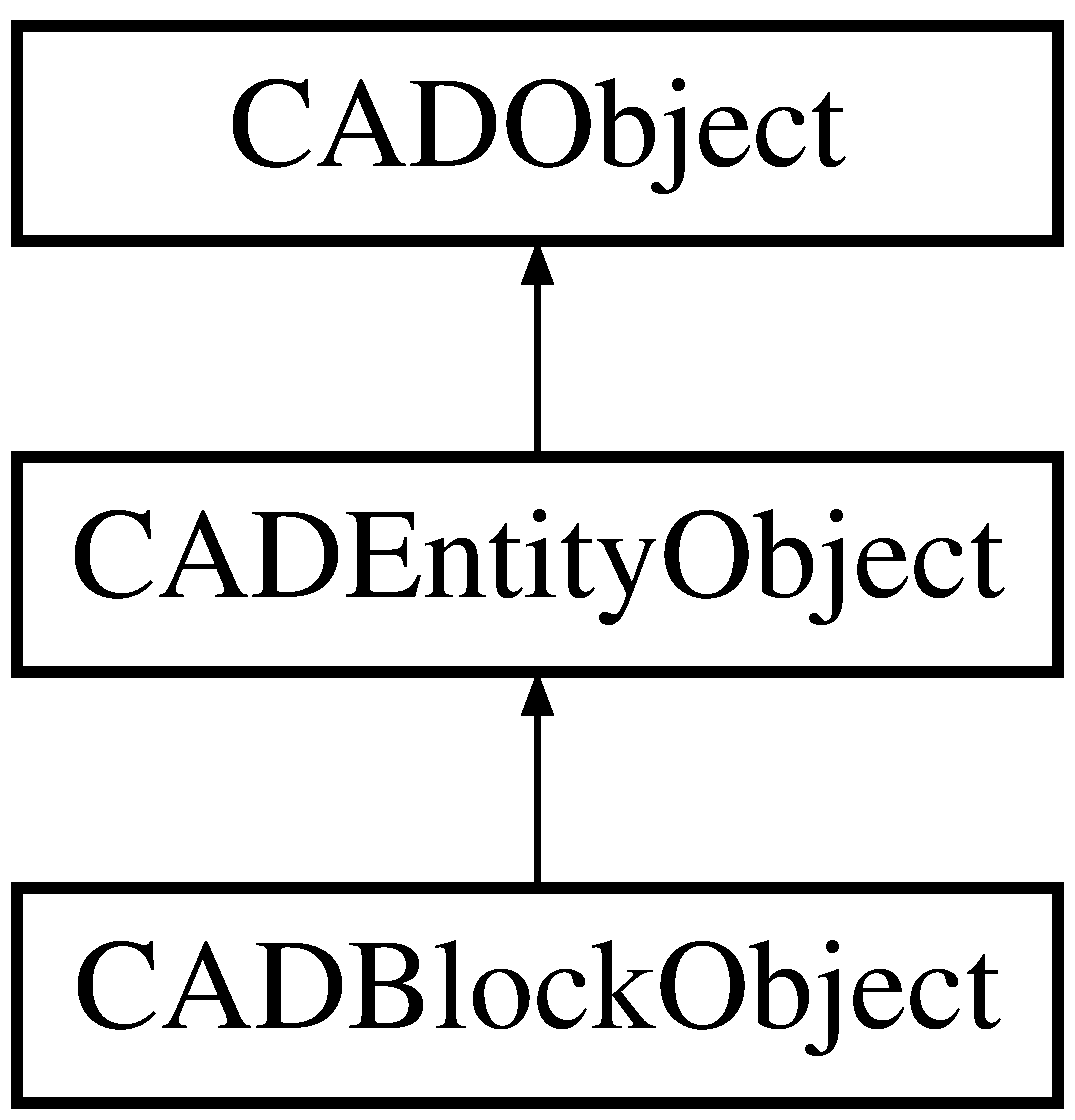
\includegraphics[height=3.000000cm]{class_c_a_d_block_object}
\end{center}
\end{figure}
\subsection*{Public Attributes}
\begin{DoxyCompactItemize}
\item 
string {\bfseries s\+Block\+Name}\hypertarget{class_c_a_d_block_object_a91f8c26aaf0a65b4a26284ae82d630f6}{}\label{class_c_a_d_block_object_a91f8c26aaf0a65b4a26284ae82d630f6}

\end{DoxyCompactItemize}
\subsection*{Additional Inherited Members}


\subsection{Detailed Description}
The C\+AD Block Object class. 

The documentation for this class was generated from the following files\+:\begin{DoxyCompactItemize}
\item 
cadobjects.\+h\item 
cadobjects.\+cpp\end{DoxyCompactItemize}

\hypertarget{class_c_a_d_circle}{}\section{C\+A\+D\+Circle Class Reference}
\label{class_c_a_d_circle}\index{C\+A\+D\+Circle@{C\+A\+D\+Circle}}


Geometry class which represents Circle.  




{\ttfamily \#include $<$cadgeometry.\+h$>$}

Inheritance diagram for C\+A\+D\+Circle\+:\begin{figure}[H]
\begin{center}
\leavevmode
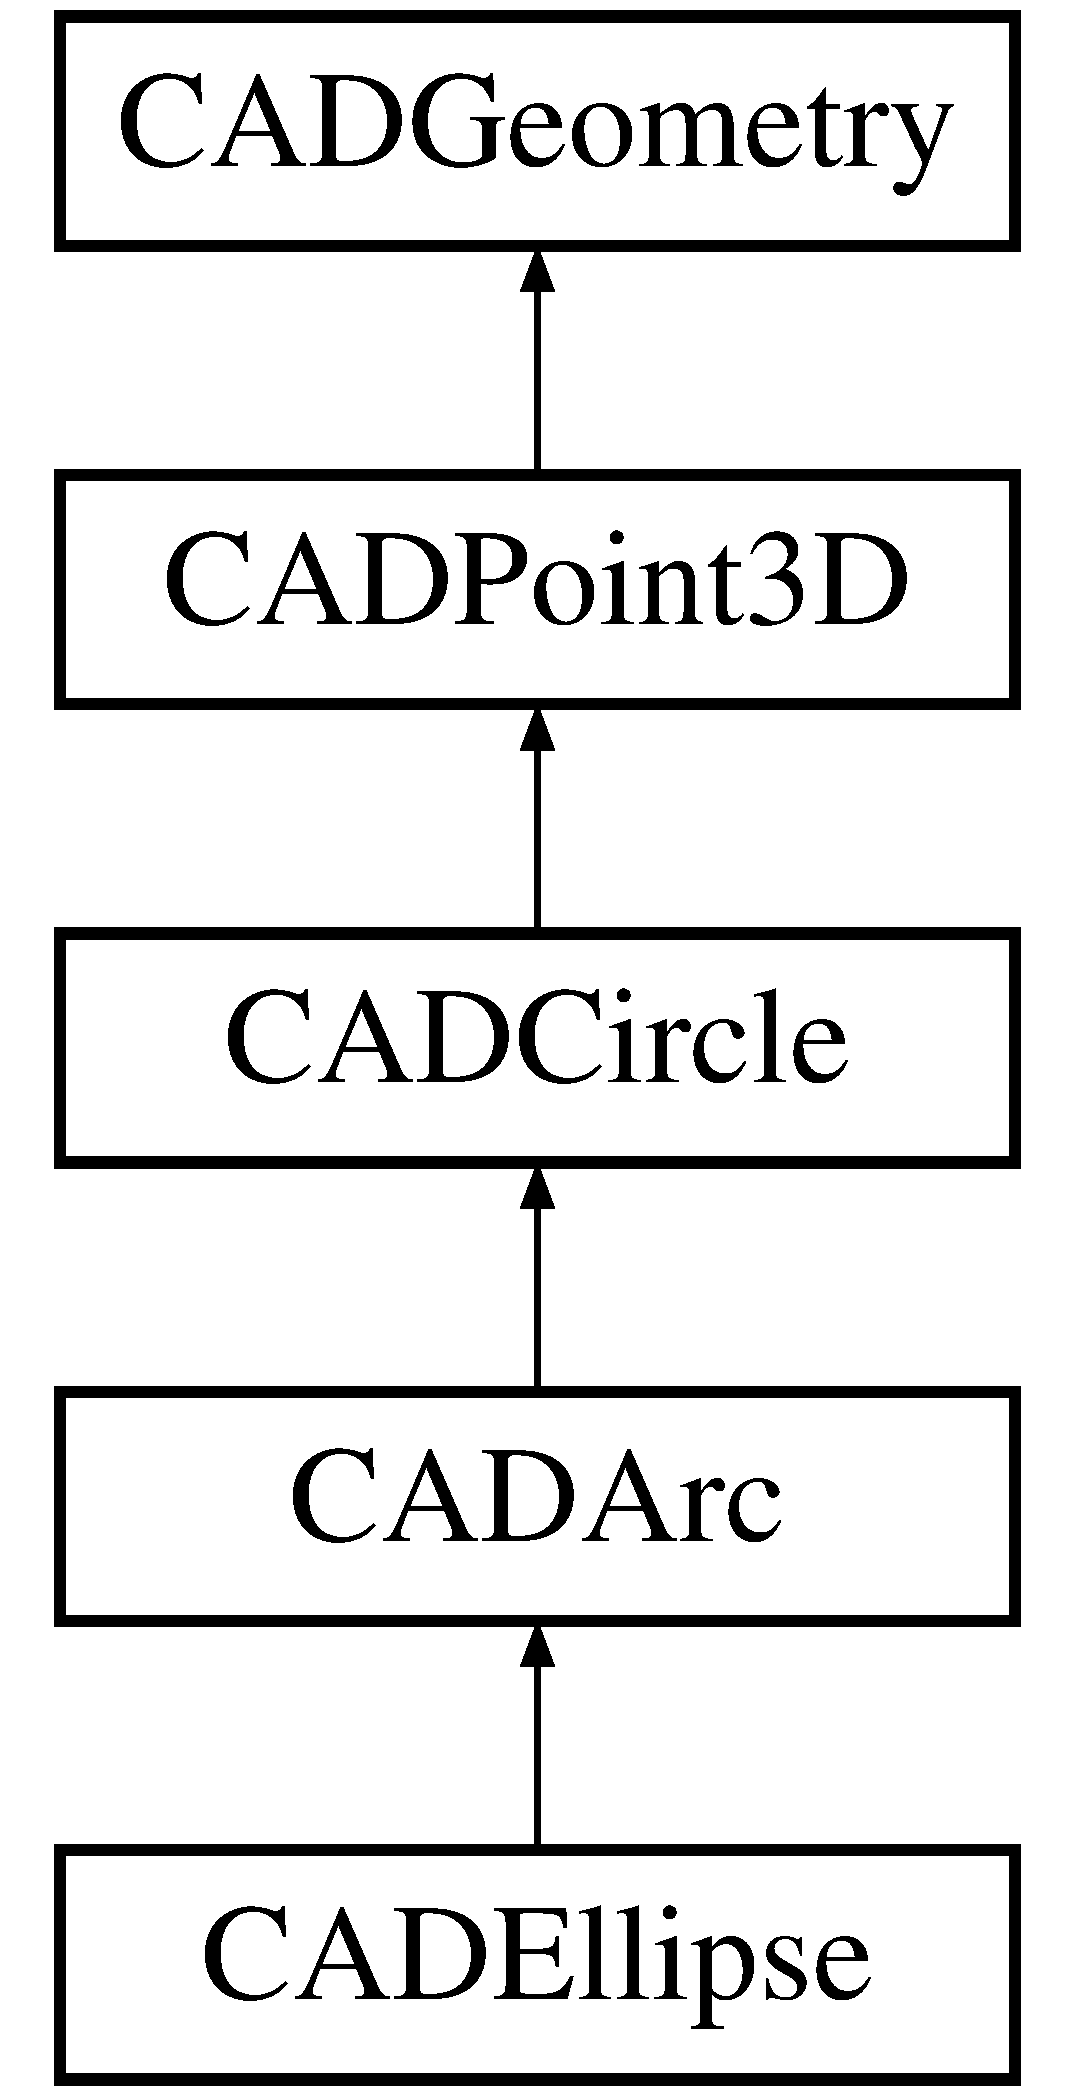
\includegraphics[height=5.000000cm]{class_c_a_d_circle}
\end{center}
\end{figure}
\subsection*{Public Member Functions}
\begin{DoxyCompactItemize}
\item 
double {\bfseries get\+Radius} () const \hypertarget{class_c_a_d_circle_afe58ed942729116553e6c3b7358d9eef}{}\label{class_c_a_d_circle_afe58ed942729116553e6c3b7358d9eef}

\item 
void {\bfseries set\+Radius} (double value)\hypertarget{class_c_a_d_circle_a9d62f92c59e13a9c4d9040c48fe319d6}{}\label{class_c_a_d_circle_a9d62f92c59e13a9c4d9040c48fe319d6}

\item 
virtual void {\bfseries print} () const  override\hypertarget{class_c_a_d_circle_a54f3a34787218b7c29b63d376c878b3f}{}\label{class_c_a_d_circle_a54f3a34787218b7c29b63d376c878b3f}

\end{DoxyCompactItemize}
\subsection*{Protected Attributes}
\begin{DoxyCompactItemize}
\item 
double {\bfseries radius}\hypertarget{class_c_a_d_circle_a56ecff7d4adf6d40712afc83e0d0216d}{}\label{class_c_a_d_circle_a56ecff7d4adf6d40712afc83e0d0216d}

\end{DoxyCompactItemize}
\subsection*{Additional Inherited Members}


\subsection{Detailed Description}
Geometry class which represents Circle. 

The documentation for this class was generated from the following files\+:\begin{DoxyCompactItemize}
\item 
cadgeometry.\+h\item 
cadgeometry.\+cpp\end{DoxyCompactItemize}

\hypertarget{class_c_a_d_circle_object}{}\section{C\+A\+D\+Circle\+Object Class Reference}
\label{class_c_a_d_circle_object}\index{C\+A\+D\+Circle\+Object@{C\+A\+D\+Circle\+Object}}


The \hyperlink{class_c_a_d_circle_object}{C\+A\+D\+Circle\+Object} class.  




{\ttfamily \#include $<$cadobjects.\+h$>$}

Inheritance diagram for C\+A\+D\+Circle\+Object\+:\begin{figure}[H]
\begin{center}
\leavevmode
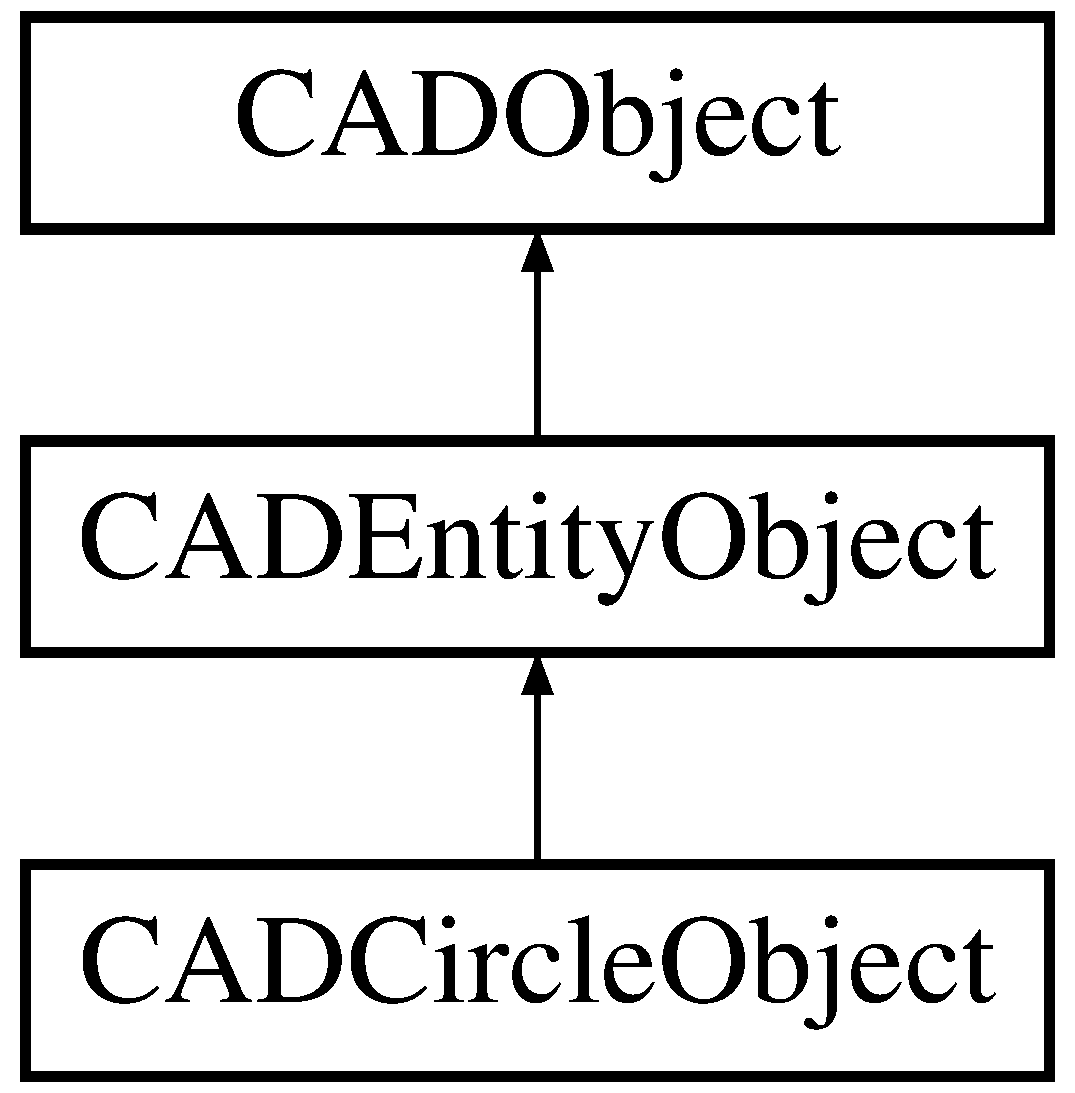
\includegraphics[height=3.000000cm]{class_c_a_d_circle_object}
\end{center}
\end{figure}
\subsection*{Public Attributes}
\begin{DoxyCompactItemize}
\item 
\hyperlink{class_c_a_d_vector}{C\+A\+D\+Vector} {\bfseries vert\+Position}\hypertarget{class_c_a_d_circle_object_a8e9f8af88cd3bbaf012b8535d91e703a}{}\label{class_c_a_d_circle_object_a8e9f8af88cd3bbaf012b8535d91e703a}

\item 
double {\bfseries df\+Radius}\hypertarget{class_c_a_d_circle_object_aa57ef49fbb95694f489f6afabae8e7f7}{}\label{class_c_a_d_circle_object_aa57ef49fbb95694f489f6afabae8e7f7}

\item 
double {\bfseries df\+Thickness}\hypertarget{class_c_a_d_circle_object_a6b4c5969fe708a4dca4e51e4e47860b6}{}\label{class_c_a_d_circle_object_a6b4c5969fe708a4dca4e51e4e47860b6}

\item 
\hyperlink{class_c_a_d_vector}{C\+A\+D\+Vector} {\bfseries vect\+Extrusion}\hypertarget{class_c_a_d_circle_object_a69866173a8fd2af7ba266c067bc75fa3}{}\label{class_c_a_d_circle_object_a69866173a8fd2af7ba266c067bc75fa3}

\end{DoxyCompactItemize}
\subsection*{Additional Inherited Members}


\subsection{Detailed Description}
The \hyperlink{class_c_a_d_circle_object}{C\+A\+D\+Circle\+Object} class. 

The documentation for this class was generated from the following files\+:\begin{DoxyCompactItemize}
\item 
cadobjects.\+h\item 
cadobjects.\+cpp\end{DoxyCompactItemize}

\hypertarget{struct_c_a_d_class}{}\section{C\+A\+D\+Class Struct Reference}
\label{struct_c_a_d_class}\index{C\+A\+D\+Class@{C\+A\+D\+Class}}
\subsection*{Public Attributes}
\begin{DoxyCompactItemize}
\item 
string \hyperlink{struct_c_a_d_class_acfca1558a652e86d0b3b73638e85da9a}{s\+Cpp\+Class\+Name}
\item 
string \hyperlink{struct_c_a_d_class_a0526e446517876d44964dc2aa1e098bc}{s\+Application\+Name}
\item 
string \hyperlink{struct_c_a_d_class_a17535310e9f4855ac640f04f037a3e63}{s\+D\+X\+F\+Record\+Name}
\item 
int \hyperlink{struct_c_a_d_class_a47022deef6fa84a4062e39a66c822ee2}{d\+Proxy\+Cap\+Flag}
\item 
unsigned short \hyperlink{struct_c_a_d_class_abcf456bcb9c603da391bd7a10dde9344}{d\+Instance\+Count}
\item 
bool \hyperlink{struct_c_a_d_class_ab628f145a66c99a6a892cc1056e55088}{b\+Was\+Zombie}
\item 
bool \hyperlink{struct_c_a_d_class_a9b1ed095dff1ff1ee00d459f1431cb32}{b\+Is\+Entity}
\item 
short {\bfseries d\+Class\+Num}\hypertarget{struct_c_a_d_class_a40f8b560c964ad5323542c8dd3441e70}{}\label{struct_c_a_d_class_a40f8b560c964ad5323542c8dd3441e70}

\item 
short {\bfseries d\+Class\+Version}\hypertarget{struct_c_a_d_class_a4b128b4da96eced4cb33dd0a76b77034}{}\label{struct_c_a_d_class_a4b128b4da96eced4cb33dd0a76b77034}

\end{DoxyCompactItemize}


\subsection{Member Data Documentation}
\index{C\+A\+D\+Class@{C\+A\+D\+Class}!b\+Is\+Entity@{b\+Is\+Entity}}
\index{b\+Is\+Entity@{b\+Is\+Entity}!C\+A\+D\+Class@{C\+A\+D\+Class}}
\subsubsection[{\texorpdfstring{b\+Is\+Entity}{bIsEntity}}]{\setlength{\rightskip}{0pt plus 5cm}bool C\+A\+D\+Class\+::b\+Is\+Entity}\hypertarget{struct_c_a_d_class_a9b1ed095dff1ff1ee00d459f1431cb32}{}\label{struct_c_a_d_class_a9b1ed095dff1ff1ee00d459f1431cb32}
B\+I\+T\+S\+H\+O\+RT, Is-\/an-\/entity flag, 281 \index{C\+A\+D\+Class@{C\+A\+D\+Class}!b\+Was\+Zombie@{b\+Was\+Zombie}}
\index{b\+Was\+Zombie@{b\+Was\+Zombie}!C\+A\+D\+Class@{C\+A\+D\+Class}}
\subsubsection[{\texorpdfstring{b\+Was\+Zombie}{bWasZombie}}]{\setlength{\rightskip}{0pt plus 5cm}bool C\+A\+D\+Class\+::b\+Was\+Zombie}\hypertarget{struct_c_a_d_class_ab628f145a66c99a6a892cc1056e55088}{}\label{struct_c_a_d_class_ab628f145a66c99a6a892cc1056e55088}
B\+IT, Was-\/a-\/proxy flag, 280 \index{C\+A\+D\+Class@{C\+A\+D\+Class}!d\+Instance\+Count@{d\+Instance\+Count}}
\index{d\+Instance\+Count@{d\+Instance\+Count}!C\+A\+D\+Class@{C\+A\+D\+Class}}
\subsubsection[{\texorpdfstring{d\+Instance\+Count}{dInstanceCount}}]{\setlength{\rightskip}{0pt plus 5cm}unsigned short C\+A\+D\+Class\+::d\+Instance\+Count}\hypertarget{struct_c_a_d_class_abcf456bcb9c603da391bd7a10dde9344}{}\label{struct_c_a_d_class_abcf456bcb9c603da391bd7a10dde9344}
B\+I\+T\+S\+H\+O\+RT, Instance count for a custom class, 91 \index{C\+A\+D\+Class@{C\+A\+D\+Class}!d\+Proxy\+Cap\+Flag@{d\+Proxy\+Cap\+Flag}}
\index{d\+Proxy\+Cap\+Flag@{d\+Proxy\+Cap\+Flag}!C\+A\+D\+Class@{C\+A\+D\+Class}}
\subsubsection[{\texorpdfstring{d\+Proxy\+Cap\+Flag}{dProxyCapFlag}}]{\setlength{\rightskip}{0pt plus 5cm}int C\+A\+D\+Class\+::d\+Proxy\+Cap\+Flag}\hypertarget{struct_c_a_d_class_a47022deef6fa84a4062e39a66c822ee2}{}\label{struct_c_a_d_class_a47022deef6fa84a4062e39a66c822ee2}
B\+I\+T\+S\+H\+O\+RT, Proxy capabilities flag, 90 \index{C\+A\+D\+Class@{C\+A\+D\+Class}!s\+Application\+Name@{s\+Application\+Name}}
\index{s\+Application\+Name@{s\+Application\+Name}!C\+A\+D\+Class@{C\+A\+D\+Class}}
\subsubsection[{\texorpdfstring{s\+Application\+Name}{sApplicationName}}]{\setlength{\rightskip}{0pt plus 5cm}string C\+A\+D\+Class\+::s\+Application\+Name}\hypertarget{struct_c_a_d_class_a0526e446517876d44964dc2aa1e098bc}{}\label{struct_c_a_d_class_a0526e446517876d44964dc2aa1e098bc}
TV, Application name \index{C\+A\+D\+Class@{C\+A\+D\+Class}!s\+Cpp\+Class\+Name@{s\+Cpp\+Class\+Name}}
\index{s\+Cpp\+Class\+Name@{s\+Cpp\+Class\+Name}!C\+A\+D\+Class@{C\+A\+D\+Class}}
\subsubsection[{\texorpdfstring{s\+Cpp\+Class\+Name}{sCppClassName}}]{\setlength{\rightskip}{0pt plus 5cm}string C\+A\+D\+Class\+::s\+Cpp\+Class\+Name}\hypertarget{struct_c_a_d_class_acfca1558a652e86d0b3b73638e85da9a}{}\label{struct_c_a_d_class_acfca1558a652e86d0b3b73638e85da9a}
TV, C++ class name \index{C\+A\+D\+Class@{C\+A\+D\+Class}!s\+D\+X\+F\+Record\+Name@{s\+D\+X\+F\+Record\+Name}}
\index{s\+D\+X\+F\+Record\+Name@{s\+D\+X\+F\+Record\+Name}!C\+A\+D\+Class@{C\+A\+D\+Class}}
\subsubsection[{\texorpdfstring{s\+D\+X\+F\+Record\+Name}{sDXFRecordName}}]{\setlength{\rightskip}{0pt plus 5cm}string C\+A\+D\+Class\+::s\+D\+X\+F\+Record\+Name}\hypertarget{struct_c_a_d_class_a17535310e9f4855ac640f04f037a3e63}{}\label{struct_c_a_d_class_a17535310e9f4855ac640f04f037a3e63}
TV, Class D\+XF record name 

The documentation for this struct was generated from the following file\+:\begin{DoxyCompactItemize}
\item 
cadclasses.\+h\end{DoxyCompactItemize}

\hypertarget{class_c_a_d_classes}{}\section{C\+A\+D\+Classes Class Reference}
\label{class_c_a_d_classes}\index{C\+A\+D\+Classes@{C\+A\+D\+Classes}}
\subsection*{Public Member Functions}
\begin{DoxyCompactItemize}
\item 
void {\bfseries add\+Class} (struct \hyperlink{struct_c_a_d_class}{C\+A\+D\+Class} st\+Class)\hypertarget{class_c_a_d_classes_a8f2833c90d00c80273398ddf67521745}{}\label{class_c_a_d_classes_a8f2833c90d00c80273398ddf67521745}

\item 
void {\bfseries print} () const \hypertarget{class_c_a_d_classes_a0d34103a182c47192ede8441c14fd290}{}\label{class_c_a_d_classes_a0d34103a182c47192ede8441c14fd290}

\end{DoxyCompactItemize}
\subsection*{Protected Attributes}
\begin{DoxyCompactItemize}
\item 
vector$<$ struct \hyperlink{struct_c_a_d_class}{C\+A\+D\+Class} $>$ {\bfseries classes}\hypertarget{class_c_a_d_classes_a0a411e3a245e3f87f4ce2e5d4f215b32}{}\label{class_c_a_d_classes_a0a411e3a245e3f87f4ce2e5d4f215b32}

\end{DoxyCompactItemize}


The documentation for this class was generated from the following files\+:\begin{DoxyCompactItemize}
\item 
cadclasses.\+h\item 
cadclasses.\+cpp\end{DoxyCompactItemize}

\hypertarget{struct_c_a_d_common_e_d}{}\section{C\+A\+D\+Common\+ED Struct Reference}
\label{struct_c_a_d_common_e_d}\index{C\+A\+D\+Common\+ED@{C\+A\+D\+Common\+ED}}


The \hyperlink{struct_c_a_d_common_e_d}{C\+A\+D\+Common\+ED} struct.  




{\ttfamily \#include $<$cadobjects.\+h$>$}

\subsection*{Public Attributes}
\begin{DoxyCompactItemize}
\item 
long {\bfseries n\+Object\+Size\+In\+Bits}\hypertarget{struct_c_a_d_common_e_d_a9680143c56cb3a1baee4248a8537e936}{}\label{struct_c_a_d_common_e_d_a9680143c56cb3a1baee4248a8537e936}

\item 
\hyperlink{class_c_a_d_handle}{C\+A\+D\+Handle} {\bfseries h\+Object\+Handle}\hypertarget{struct_c_a_d_common_e_d_a53c624ede9eb300b372c606f94d1b980}{}\label{struct_c_a_d_common_e_d_a53c624ede9eb300b372c606f94d1b980}

\item 
C\+A\+D\+Eed\+Array {\bfseries a\+E\+ED}\hypertarget{struct_c_a_d_common_e_d_a2670cd399e0557fc573689bd83fabff1}{}\label{struct_c_a_d_common_e_d_a2670cd399e0557fc573689bd83fabff1}

\item 
bool {\bfseries b\+Graphics\+Presented}\hypertarget{struct_c_a_d_common_e_d_acff0cd1ce191a0305b2b53cffa209a49}{}\label{struct_c_a_d_common_e_d_acff0cd1ce191a0305b2b53cffa209a49}

\item 
vector$<$ char $>$ {\bfseries aby\+Graphics\+Data}\hypertarget{struct_c_a_d_common_e_d_a9927124f326875ab452754fec0582a9d}{}\label{struct_c_a_d_common_e_d_a9927124f326875ab452754fec0582a9d}

\item 
unsigned char {\bfseries bb\+Ent\+Mode}\hypertarget{struct_c_a_d_common_e_d_a43e43cc4103ce1b8b65d7433cf111484}{}\label{struct_c_a_d_common_e_d_a43e43cc4103ce1b8b65d7433cf111484}

\item 
long {\bfseries n\+Num\+Reactors}\hypertarget{struct_c_a_d_common_e_d_a4d1076b75583f9e2f9f3ee2a497e7bc1}{}\label{struct_c_a_d_common_e_d_a4d1076b75583f9e2f9f3ee2a497e7bc1}

\item 
bool {\bfseries b\+No\+X\+Dictionary\+Handle\+Present}\hypertarget{struct_c_a_d_common_e_d_a09a0803450ed6e6d96aaef3566e60baa}{}\label{struct_c_a_d_common_e_d_a09a0803450ed6e6d96aaef3566e60baa}

\item 
bool {\bfseries b\+Binary\+Data\+Present}\hypertarget{struct_c_a_d_common_e_d_a4abd25870f24a17f3b884df75c6f3f57}{}\label{struct_c_a_d_common_e_d_a4abd25870f24a17f3b884df75c6f3f57}

\item 
bool {\bfseries b\+Is\+By\+Layer\+LT}\hypertarget{struct_c_a_d_common_e_d_ad93433415d0c852b199f733cb8a7bef5}{}\label{struct_c_a_d_common_e_d_ad93433415d0c852b199f733cb8a7bef5}

\item 
bool {\bfseries b\+No\+Links}\hypertarget{struct_c_a_d_common_e_d_a5542a7b6a6a2cf8e0d7467a254bfc3fc}{}\label{struct_c_a_d_common_e_d_a5542a7b6a6a2cf8e0d7467a254bfc3fc}

\item 
short {\bfseries n\+C\+M\+Color}\hypertarget{struct_c_a_d_common_e_d_a4d1245beb992537767b9e2c733ab5cf0}{}\label{struct_c_a_d_common_e_d_a4d1245beb992537767b9e2c733ab5cf0}

\item 
double {\bfseries df\+L\+Type\+Scale}\hypertarget{struct_c_a_d_common_e_d_a8258666386879878ead9605945c63ea1}{}\label{struct_c_a_d_common_e_d_a8258666386879878ead9605945c63ea1}

\item 
unsigned char {\bfseries bb\+L\+Type\+Flags}\hypertarget{struct_c_a_d_common_e_d_aa0458ddeda2f22962dfbe1b3d06fbddc}{}\label{struct_c_a_d_common_e_d_aa0458ddeda2f22962dfbe1b3d06fbddc}

\item 
unsigned char {\bfseries bb\+Plot\+Style\+Flags}\hypertarget{struct_c_a_d_common_e_d_a7908da9db207d6f15529a83ec5c668fd}{}\label{struct_c_a_d_common_e_d_a7908da9db207d6f15529a83ec5c668fd}

\item 
char {\bfseries bb\+Material\+Flags}\hypertarget{struct_c_a_d_common_e_d_aea1300df157342ad445041e8597e6034}{}\label{struct_c_a_d_common_e_d_aea1300df157342ad445041e8597e6034}

\item 
char {\bfseries n\+Shadow\+Flags}\hypertarget{struct_c_a_d_common_e_d_a31eaf5987612ba658d269c10d6a86599}{}\label{struct_c_a_d_common_e_d_a31eaf5987612ba658d269c10d6a86599}

\item 
short {\bfseries n\+Invisibility}\hypertarget{struct_c_a_d_common_e_d_aa6b75a63cc5627a026fc685cc6c61ce4}{}\label{struct_c_a_d_common_e_d_aa6b75a63cc5627a026fc685cc6c61ce4}

\item 
unsigned char {\bfseries n\+Line\+Weight}\hypertarget{struct_c_a_d_common_e_d_a6188e6801d929cf163fb7b710394a13d}{}\label{struct_c_a_d_common_e_d_a6188e6801d929cf163fb7b710394a13d}

\end{DoxyCompactItemize}


\subsection{Detailed Description}
The \hyperlink{struct_c_a_d_common_e_d}{C\+A\+D\+Common\+ED} struct. 

The documentation for this struct was generated from the following file\+:\begin{DoxyCompactItemize}
\item 
cadobjects.\+h\end{DoxyCompactItemize}

\hypertarget{struct_c_a_d_common_e_h_d}{}\section{C\+A\+D\+Common\+E\+HD Struct Reference}
\label{struct_c_a_d_common_e_h_d}\index{C\+A\+D\+Common\+E\+HD@{C\+A\+D\+Common\+E\+HD}}


The \hyperlink{struct_c_a_d_common_e_h_d}{C\+A\+D\+Common\+E\+HD} struct.  




{\ttfamily \#include $<$cadobjects.\+h$>$}

\subsection*{Public Attributes}
\begin{DoxyCompactItemize}
\item 
\hyperlink{class_c_a_d_handle}{C\+A\+D\+Handle} {\bfseries h\+Owner}\hypertarget{struct_c_a_d_common_e_h_d_a0b9dcdf756bad0aff764237fe5ef5fac}{}\label{struct_c_a_d_common_e_h_d_a0b9dcdf756bad0aff764237fe5ef5fac}

\item 
C\+A\+D\+Handle\+Array {\bfseries h\+Reactors}\hypertarget{struct_c_a_d_common_e_h_d_a89af01530bd391751584cde5558ffaf5}{}\label{struct_c_a_d_common_e_h_d_a89af01530bd391751584cde5558ffaf5}

\item 
\hyperlink{class_c_a_d_handle}{C\+A\+D\+Handle} {\bfseries h\+X\+Dictionary}\hypertarget{struct_c_a_d_common_e_h_d_aeaac24d666157eae151e7f558ce3cb91}{}\label{struct_c_a_d_common_e_h_d_aeaac24d666157eae151e7f558ce3cb91}

\item 
\hyperlink{class_c_a_d_handle}{C\+A\+D\+Handle} {\bfseries h\+Layer}\hypertarget{struct_c_a_d_common_e_h_d_a722a59e32339573b60355475a4eb77c9}{}\label{struct_c_a_d_common_e_h_d_a722a59e32339573b60355475a4eb77c9}

\item 
\hyperlink{class_c_a_d_handle}{C\+A\+D\+Handle} {\bfseries h\+L\+Type}\hypertarget{struct_c_a_d_common_e_h_d_a8e322b6906d77b6e87f20e7676255aaa}{}\label{struct_c_a_d_common_e_h_d_a8e322b6906d77b6e87f20e7676255aaa}

\item 
\hyperlink{class_c_a_d_handle}{C\+A\+D\+Handle} {\bfseries h\+Prev\+Entity}\hypertarget{struct_c_a_d_common_e_h_d_a10d85f618c0428bfb8833af629f6be10}{}\label{struct_c_a_d_common_e_h_d_a10d85f618c0428bfb8833af629f6be10}

\item 
\hyperlink{class_c_a_d_handle}{C\+A\+D\+Handle} {\bfseries h\+Next\+Entity}\hypertarget{struct_c_a_d_common_e_h_d_ac566a87a33ed49b272b8647fcd54a4b7}{}\label{struct_c_a_d_common_e_h_d_ac566a87a33ed49b272b8647fcd54a4b7}

\item 
\hyperlink{class_c_a_d_handle}{C\+A\+D\+Handle} {\bfseries h\+Color\+Book\+Handle}\hypertarget{struct_c_a_d_common_e_h_d_a94a69a18e50c11a6d08ab9cd23ffafe5}{}\label{struct_c_a_d_common_e_h_d_a94a69a18e50c11a6d08ab9cd23ffafe5}

\item 
\hyperlink{class_c_a_d_handle}{C\+A\+D\+Handle} {\bfseries h\+Material}\hypertarget{struct_c_a_d_common_e_h_d_a9ebf2ff0ac69686bd6d818362245021d}{}\label{struct_c_a_d_common_e_h_d_a9ebf2ff0ac69686bd6d818362245021d}

\item 
\hyperlink{class_c_a_d_handle}{C\+A\+D\+Handle} {\bfseries h\+Plot\+Style}\hypertarget{struct_c_a_d_common_e_h_d_afe482d65b2cba4333eb074f8aa4408f6}{}\label{struct_c_a_d_common_e_h_d_afe482d65b2cba4333eb074f8aa4408f6}

\item 
\hyperlink{class_c_a_d_handle}{C\+A\+D\+Handle} {\bfseries h\+Full\+Visual\+Style}\hypertarget{struct_c_a_d_common_e_h_d_a8f04a2c251fe0d108bb15af536a31420}{}\label{struct_c_a_d_common_e_h_d_a8f04a2c251fe0d108bb15af536a31420}

\item 
\hyperlink{class_c_a_d_handle}{C\+A\+D\+Handle} {\bfseries h\+Face\+Visual\+Style}\hypertarget{struct_c_a_d_common_e_h_d_ae6f83c99d7023cc1634abd0709fb48c3}{}\label{struct_c_a_d_common_e_h_d_ae6f83c99d7023cc1634abd0709fb48c3}

\item 
\hyperlink{class_c_a_d_handle}{C\+A\+D\+Handle} {\bfseries h\+Edge\+Visual\+Style}\hypertarget{struct_c_a_d_common_e_h_d_aab85327e9b9917642286489ec5ae903f}{}\label{struct_c_a_d_common_e_h_d_aab85327e9b9917642286489ec5ae903f}

\end{DoxyCompactItemize}


\subsection{Detailed Description}
The \hyperlink{struct_c_a_d_common_e_h_d}{C\+A\+D\+Common\+E\+HD} struct. 

The documentation for this struct was generated from the following file\+:\begin{DoxyCompactItemize}
\item 
cadobjects.\+h\end{DoxyCompactItemize}

\hypertarget{class_c_a_d_dictionary_object}{}\section{C\+A\+D\+Dictionary\+Object Class Reference}
\label{class_c_a_d_dictionary_object}\index{C\+A\+D\+Dictionary\+Object@{C\+A\+D\+Dictionary\+Object}}


The \hyperlink{class_c_a_d_dictionary_object}{C\+A\+D\+Dictionary\+Object} class.  




{\ttfamily \#include $<$cadobjects.\+h$>$}

Inheritance diagram for C\+A\+D\+Dictionary\+Object\+:\begin{figure}[H]
\begin{center}
\leavevmode
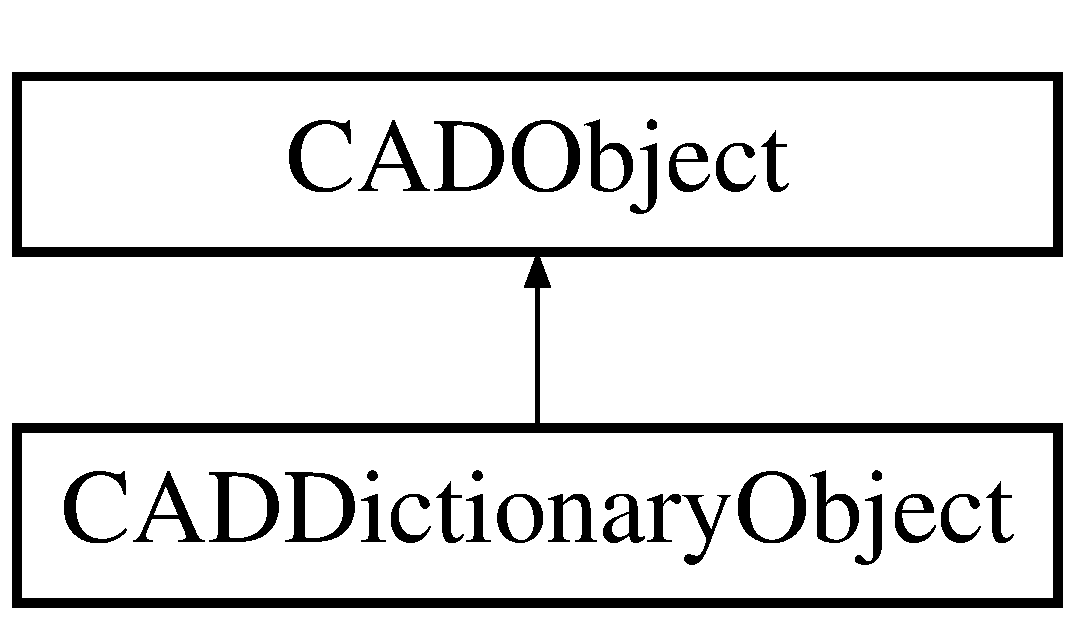
\includegraphics[height=2.000000cm]{class_c_a_d_dictionary_object}
\end{center}
\end{figure}
\subsection*{Public Attributes}
\begin{DoxyCompactItemize}
\item 
long {\bfseries n\+Object\+Size\+In\+Bits}\hypertarget{class_c_a_d_dictionary_object_a26cdcfea871cff14c39ea057cd79a9a2}{}\label{class_c_a_d_dictionary_object_a26cdcfea871cff14c39ea057cd79a9a2}

\item 
\hyperlink{class_c_a_d_handle}{C\+A\+D\+Handle} {\bfseries h\+Object\+Handle}\hypertarget{class_c_a_d_dictionary_object_acfa37cdfcdb7d693f5da1453f33249e8}{}\label{class_c_a_d_dictionary_object_acfa37cdfcdb7d693f5da1453f33249e8}

\item 
C\+A\+D\+Eed\+Array {\bfseries a\+E\+ED}\hypertarget{class_c_a_d_dictionary_object_a99c594443253ae4e5b56c9dba2501200}{}\label{class_c_a_d_dictionary_object_a99c594443253ae4e5b56c9dba2501200}

\item 
long {\bfseries n\+Num\+Reactors}\hypertarget{class_c_a_d_dictionary_object_a3af17a5f55663fb68e7cca32896977c4}{}\label{class_c_a_d_dictionary_object_a3af17a5f55663fb68e7cca32896977c4}

\item 
bool {\bfseries b\+No\+X\+Dictionary\+Present}\hypertarget{class_c_a_d_dictionary_object_a60376bbdaf2e377b81a0a7b9b9d12c7a}{}\label{class_c_a_d_dictionary_object_a60376bbdaf2e377b81a0a7b9b9d12c7a}

\item 
long {\bfseries n\+Num\+Items}\hypertarget{class_c_a_d_dictionary_object_a2fd499dec103659918698b4ab7ca45d1}{}\label{class_c_a_d_dictionary_object_a2fd499dec103659918698b4ab7ca45d1}

\item 
short {\bfseries d\+Cloning\+Flag}\hypertarget{class_c_a_d_dictionary_object_a949e5685f1e35148e90c9cee1d1561aa}{}\label{class_c_a_d_dictionary_object_a949e5685f1e35148e90c9cee1d1561aa}

\item 
unsigned char {\bfseries d\+Hard\+Owner\+Flag}\hypertarget{class_c_a_d_dictionary_object_a25a6398e019c47c98afb4e1776720276}{}\label{class_c_a_d_dictionary_object_a25a6398e019c47c98afb4e1776720276}

\item 
string {\bfseries s\+Dictionary\+Entry\+Name}\hypertarget{class_c_a_d_dictionary_object_a0e28dd0cb47703a774ebcfdeb3e80bc7}{}\label{class_c_a_d_dictionary_object_a0e28dd0cb47703a774ebcfdeb3e80bc7}

\item 
vector$<$ string $>$ {\bfseries s\+Item\+Names}\hypertarget{class_c_a_d_dictionary_object_a2a2897eebfaa60a08887dbe3025b5615}{}\label{class_c_a_d_dictionary_object_a2a2897eebfaa60a08887dbe3025b5615}

\item 
\hyperlink{class_c_a_d_handle}{C\+A\+D\+Handle} {\bfseries h\+Parent\+Handle}\hypertarget{class_c_a_d_dictionary_object_af2a49e3c2ec3fed715474196c6d4c5cb}{}\label{class_c_a_d_dictionary_object_af2a49e3c2ec3fed715474196c6d4c5cb}

\item 
C\+A\+D\+Handle\+Array {\bfseries h\+Reactors}\hypertarget{class_c_a_d_dictionary_object_ace9015530796ea736e243bd362169cc8}{}\label{class_c_a_d_dictionary_object_ace9015530796ea736e243bd362169cc8}

\item 
\hyperlink{class_c_a_d_handle}{C\+A\+D\+Handle} {\bfseries h\+X\+Dictionary}\hypertarget{class_c_a_d_dictionary_object_a559e579e28252978652f9d43846e7a9e}{}\label{class_c_a_d_dictionary_object_a559e579e28252978652f9d43846e7a9e}

\item 
C\+A\+D\+Handle\+Array {\bfseries h\+Item\+Handles}\hypertarget{class_c_a_d_dictionary_object_a5bcb01a52775ba22a75f540a4be952e0}{}\label{class_c_a_d_dictionary_object_a5bcb01a52775ba22a75f540a4be952e0}

\end{DoxyCompactItemize}
\subsection*{Additional Inherited Members}


\subsection{Detailed Description}
The \hyperlink{class_c_a_d_dictionary_object}{C\+A\+D\+Dictionary\+Object} class. 

The documentation for this class was generated from the following files\+:\begin{DoxyCompactItemize}
\item 
cadobjects.\+h\item 
cadobjects.\+cpp\end{DoxyCompactItemize}

\hypertarget{class_c_a_d_dimension_aligned_object}{}\section{C\+A\+D\+Dimension\+Aligned\+Object Class Reference}
\label{class_c_a_d_dimension_aligned_object}\index{C\+A\+D\+Dimension\+Aligned\+Object@{C\+A\+D\+Dimension\+Aligned\+Object}}


The \hyperlink{class_c_a_d_dimension_aligned_object}{C\+A\+D\+Dimension\+Aligned\+Object} class.  




{\ttfamily \#include $<$cadobjects.\+h$>$}

Inheritance diagram for C\+A\+D\+Dimension\+Aligned\+Object\+:\begin{figure}[H]
\begin{center}
\leavevmode
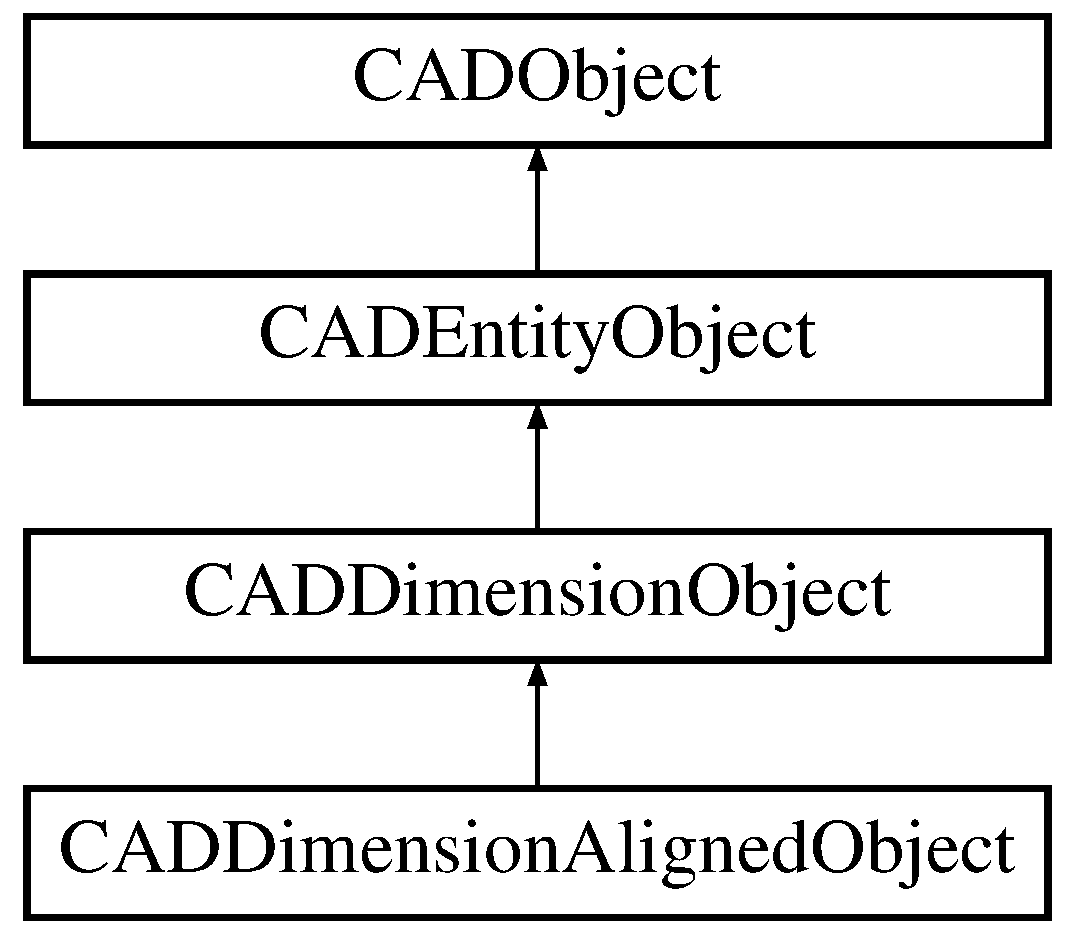
\includegraphics[height=4.000000cm]{class_c_a_d_dimension_aligned_object}
\end{center}
\end{figure}
\subsection*{Public Attributes}
\begin{DoxyCompactItemize}
\item 
\hyperlink{class_c_a_d_vector}{C\+A\+D\+Vector} {\bfseries vert13pt}\hypertarget{class_c_a_d_dimension_aligned_object_adce80725cde5678e9729d1342d6cbca5}{}\label{class_c_a_d_dimension_aligned_object_adce80725cde5678e9729d1342d6cbca5}

\item 
\hyperlink{class_c_a_d_vector}{C\+A\+D\+Vector} {\bfseries vert14pt}\hypertarget{class_c_a_d_dimension_aligned_object_a10afecff9907e633333b3f1aa3185e84}{}\label{class_c_a_d_dimension_aligned_object_a10afecff9907e633333b3f1aa3185e84}

\item 
double {\bfseries df\+Ext\+Ln\+Rot}\hypertarget{class_c_a_d_dimension_aligned_object_a1a7312e5e67400285cbff77eff27b068}{}\label{class_c_a_d_dimension_aligned_object_a1a7312e5e67400285cbff77eff27b068}

\end{DoxyCompactItemize}
\subsection*{Additional Inherited Members}


\subsection{Detailed Description}
The \hyperlink{class_c_a_d_dimension_aligned_object}{C\+A\+D\+Dimension\+Aligned\+Object} class. 

The documentation for this class was generated from the following files\+:\begin{DoxyCompactItemize}
\item 
cadobjects.\+h\item 
cadobjects.\+cpp\end{DoxyCompactItemize}

\hypertarget{class_c_a_d_dimension_angular2_ln_object}{}\section{C\+A\+D\+Dimension\+Angular2\+Ln\+Object Class Reference}
\label{class_c_a_d_dimension_angular2_ln_object}\index{C\+A\+D\+Dimension\+Angular2\+Ln\+Object@{C\+A\+D\+Dimension\+Angular2\+Ln\+Object}}


The \hyperlink{class_c_a_d_dimension_angular2_ln_object}{C\+A\+D\+Dimension\+Angular2\+Ln\+Object} class.  




{\ttfamily \#include $<$cadobjects.\+h$>$}

Inheritance diagram for C\+A\+D\+Dimension\+Angular2\+Ln\+Object\+:\begin{figure}[H]
\begin{center}
\leavevmode
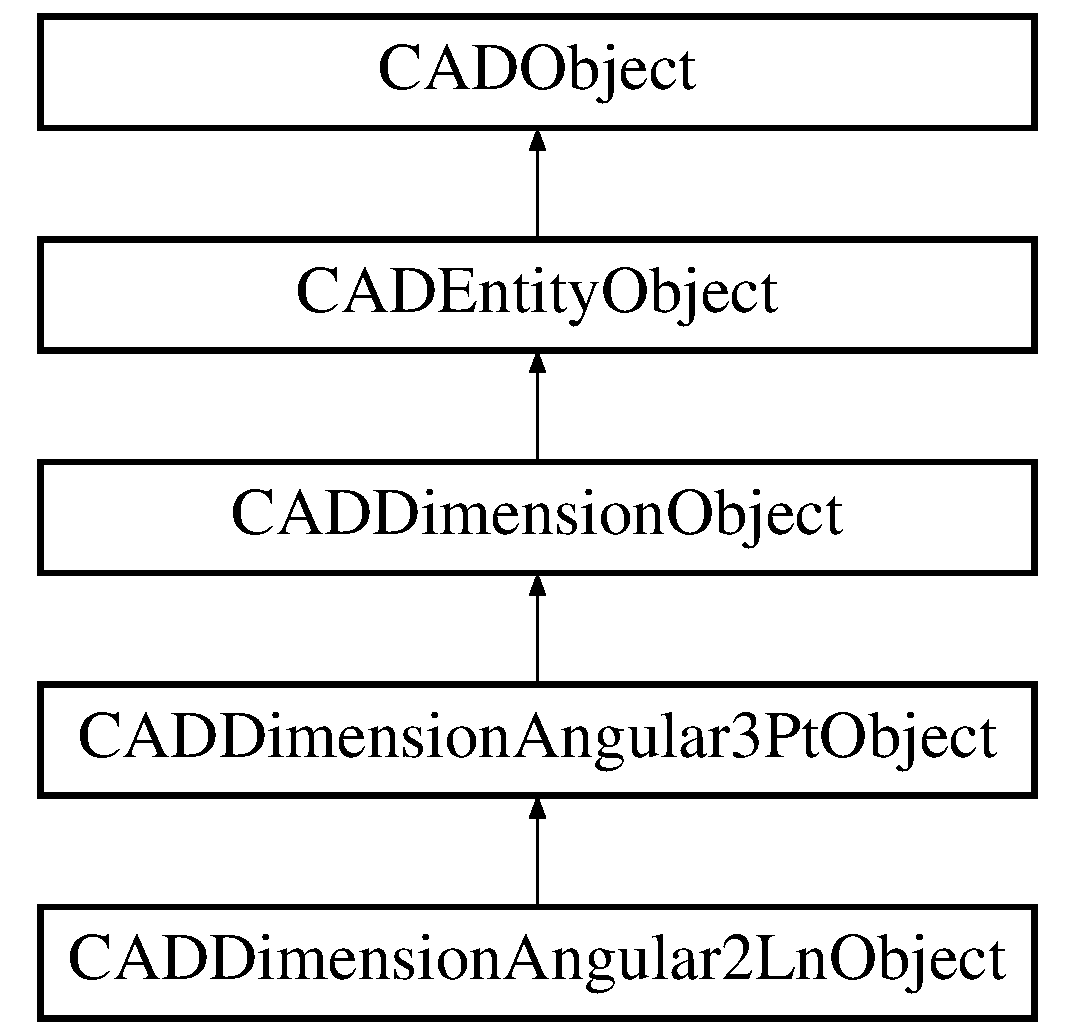
\includegraphics[height=5.000000cm]{class_c_a_d_dimension_angular2_ln_object}
\end{center}
\end{figure}
\subsection*{Public Attributes}
\begin{DoxyCompactItemize}
\item 
\hyperlink{class_c_a_d_vector}{C\+A\+D\+Vector} {\bfseries vert16pt}\hypertarget{class_c_a_d_dimension_angular2_ln_object_a34e20b39eed39d22ad7ab874a4122be3}{}\label{class_c_a_d_dimension_angular2_ln_object_a34e20b39eed39d22ad7ab874a4122be3}

\end{DoxyCompactItemize}
\subsection*{Additional Inherited Members}


\subsection{Detailed Description}
The \hyperlink{class_c_a_d_dimension_angular2_ln_object}{C\+A\+D\+Dimension\+Angular2\+Ln\+Object} class. 

The documentation for this class was generated from the following files\+:\begin{DoxyCompactItemize}
\item 
cadobjects.\+h\item 
cadobjects.\+cpp\end{DoxyCompactItemize}

\hypertarget{class_c_a_d_dimension_angular3_pt_object}{}\section{C\+A\+D\+Dimension\+Angular3\+Pt\+Object Class Reference}
\label{class_c_a_d_dimension_angular3_pt_object}\index{C\+A\+D\+Dimension\+Angular3\+Pt\+Object@{C\+A\+D\+Dimension\+Angular3\+Pt\+Object}}


The \hyperlink{class_c_a_d_dimension_angular3_pt_object}{C\+A\+D\+Dimension\+Angular3\+Pt\+Object} class.  




{\ttfamily \#include $<$cadobjects.\+h$>$}

Inheritance diagram for C\+A\+D\+Dimension\+Angular3\+Pt\+Object\+:\begin{figure}[H]
\begin{center}
\leavevmode
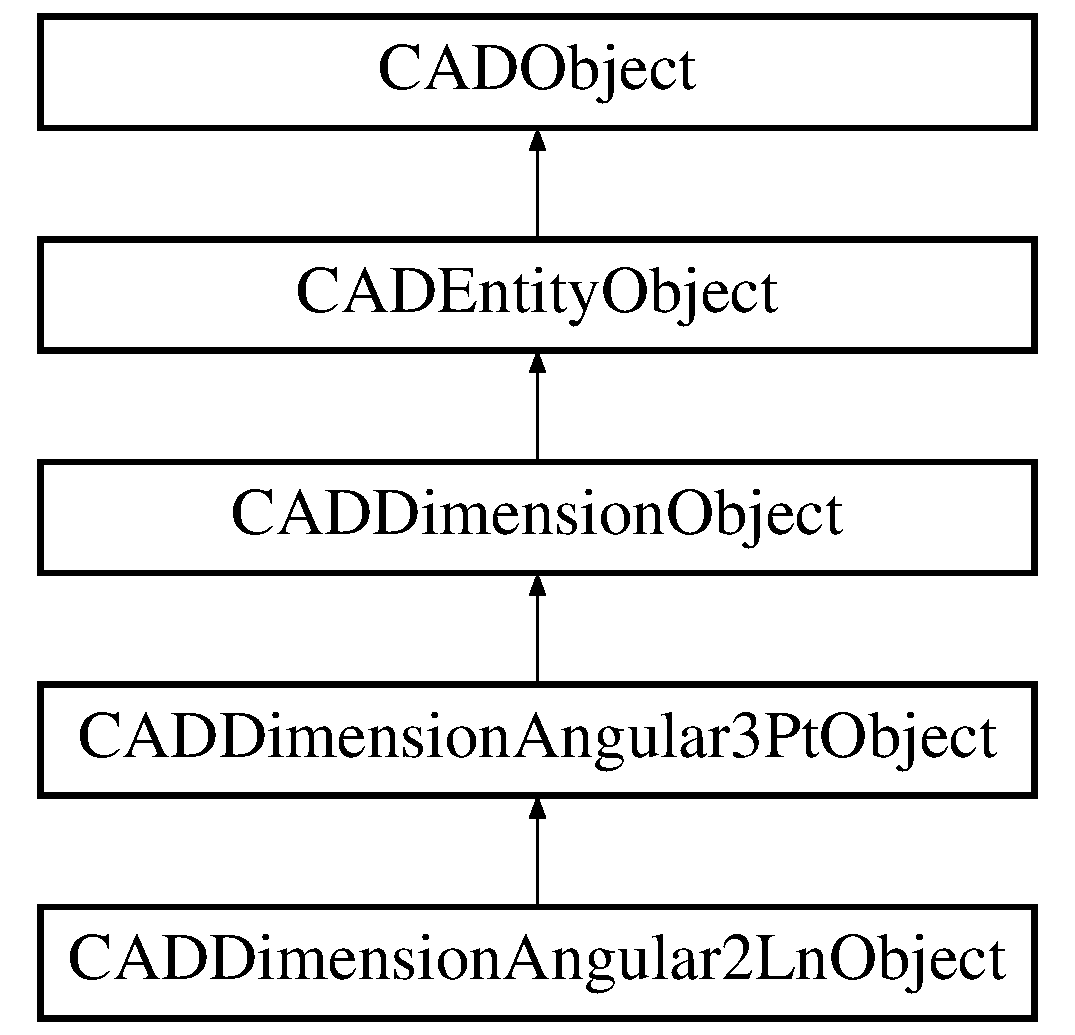
\includegraphics[height=5.000000cm]{class_c_a_d_dimension_angular3_pt_object}
\end{center}
\end{figure}
\subsection*{Public Attributes}
\begin{DoxyCompactItemize}
\item 
\hyperlink{class_c_a_d_vector}{C\+A\+D\+Vector} {\bfseries vert13pt}\hypertarget{class_c_a_d_dimension_angular3_pt_object_ace0e55e86f30e603c998b6adbf233584}{}\label{class_c_a_d_dimension_angular3_pt_object_ace0e55e86f30e603c998b6adbf233584}

\item 
\hyperlink{class_c_a_d_vector}{C\+A\+D\+Vector} {\bfseries vert14pt}\hypertarget{class_c_a_d_dimension_angular3_pt_object_a31fb70168881a8f5675a62d37f4aa16b}{}\label{class_c_a_d_dimension_angular3_pt_object_a31fb70168881a8f5675a62d37f4aa16b}

\item 
\hyperlink{class_c_a_d_vector}{C\+A\+D\+Vector} {\bfseries vert15pt}\hypertarget{class_c_a_d_dimension_angular3_pt_object_aa3db7ff197556d336112fee3c3b845c1}{}\label{class_c_a_d_dimension_angular3_pt_object_aa3db7ff197556d336112fee3c3b845c1}

\end{DoxyCompactItemize}
\subsection*{Additional Inherited Members}


\subsection{Detailed Description}
The \hyperlink{class_c_a_d_dimension_angular3_pt_object}{C\+A\+D\+Dimension\+Angular3\+Pt\+Object} class. 

The documentation for this class was generated from the following files\+:\begin{DoxyCompactItemize}
\item 
cadobjects.\+h\item 
cadobjects.\+cpp\end{DoxyCompactItemize}

\hypertarget{class_c_a_d_dimension_diameter_object}{}\section{C\+A\+D\+Dimension\+Diameter\+Object Class Reference}
\label{class_c_a_d_dimension_diameter_object}\index{C\+A\+D\+Dimension\+Diameter\+Object@{C\+A\+D\+Dimension\+Diameter\+Object}}


The \hyperlink{class_c_a_d_dimension_diameter_object}{C\+A\+D\+Dimension\+Diameter\+Object} class.  




{\ttfamily \#include $<$cadobjects.\+h$>$}

Inheritance diagram for C\+A\+D\+Dimension\+Diameter\+Object\+:\begin{figure}[H]
\begin{center}
\leavevmode
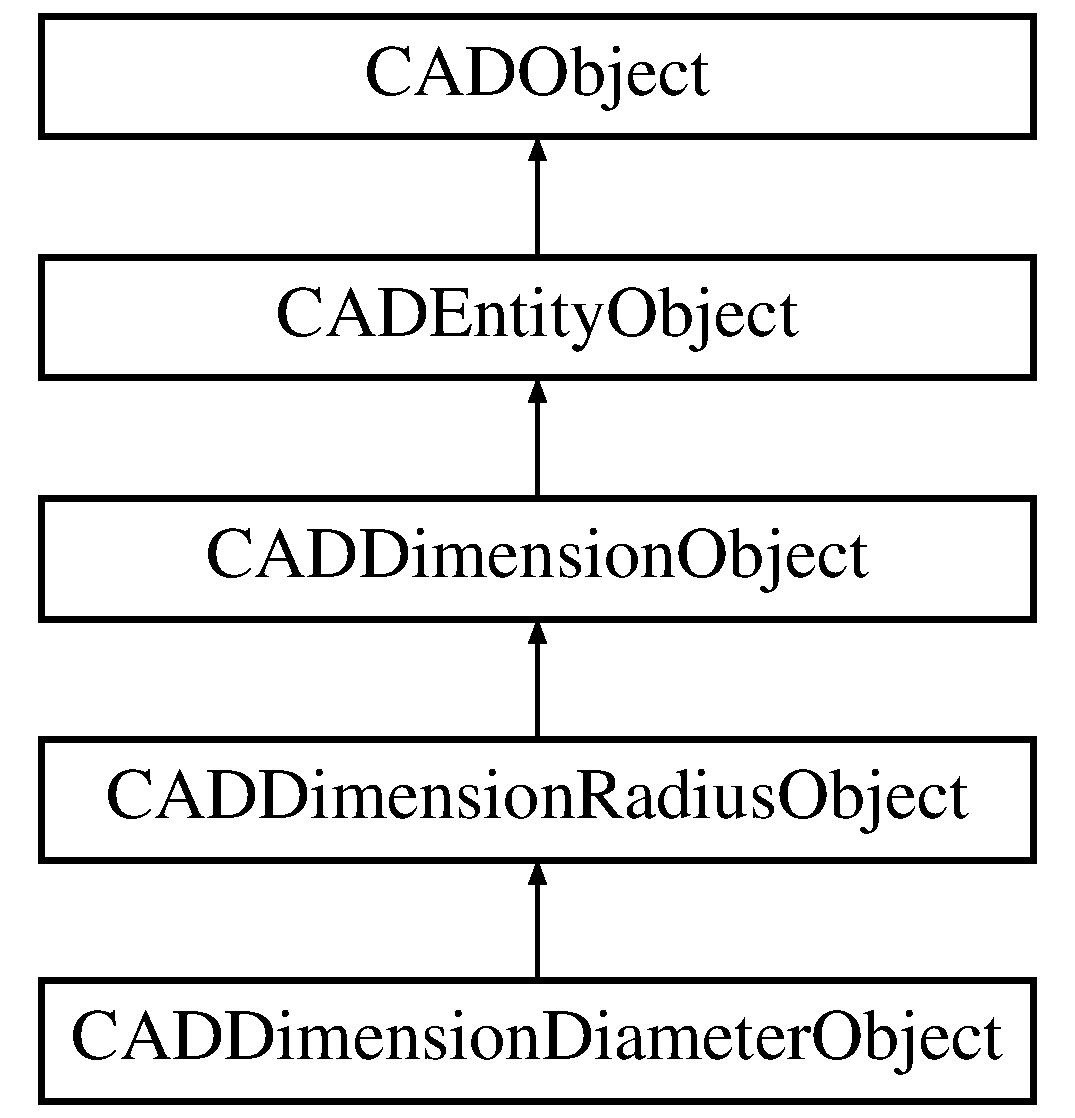
\includegraphics[height=5.000000cm]{class_c_a_d_dimension_diameter_object}
\end{center}
\end{figure}
\subsection*{Additional Inherited Members}


\subsection{Detailed Description}
The \hyperlink{class_c_a_d_dimension_diameter_object}{C\+A\+D\+Dimension\+Diameter\+Object} class. 

The documentation for this class was generated from the following files\+:\begin{DoxyCompactItemize}
\item 
cadobjects.\+h\item 
cadobjects.\+cpp\end{DoxyCompactItemize}

\hypertarget{class_c_a_d_dimension_linear_object}{}\section{C\+A\+D\+Dimension\+Linear\+Object Class Reference}
\label{class_c_a_d_dimension_linear_object}\index{C\+A\+D\+Dimension\+Linear\+Object@{C\+A\+D\+Dimension\+Linear\+Object}}


The \hyperlink{class_c_a_d_dimension_linear_object}{C\+A\+D\+Dimension\+Linear\+Object} class.  




{\ttfamily \#include $<$cadobjects.\+h$>$}

Inheritance diagram for C\+A\+D\+Dimension\+Linear\+Object\+:\begin{figure}[H]
\begin{center}
\leavevmode
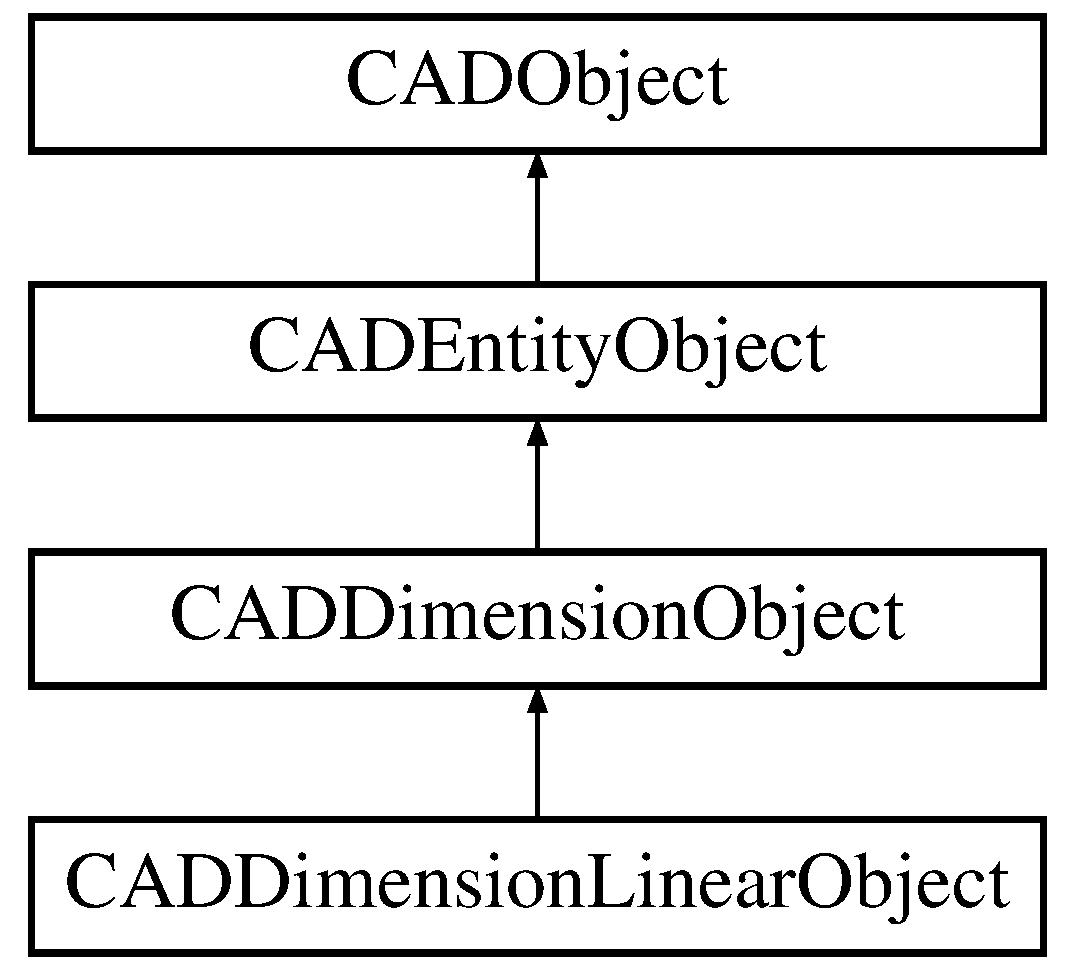
\includegraphics[height=4.000000cm]{class_c_a_d_dimension_linear_object}
\end{center}
\end{figure}
\subsection*{Public Attributes}
\begin{DoxyCompactItemize}
\item 
\hyperlink{class_c_a_d_vector}{C\+A\+D\+Vector} {\bfseries vert13pt}\hypertarget{class_c_a_d_dimension_linear_object_a78fd608b35b8c7f4ecc8f70847284b0a}{}\label{class_c_a_d_dimension_linear_object_a78fd608b35b8c7f4ecc8f70847284b0a}

\item 
\hyperlink{class_c_a_d_vector}{C\+A\+D\+Vector} {\bfseries vert14pt}\hypertarget{class_c_a_d_dimension_linear_object_ac18334779c4a44c130103f16561af5f7}{}\label{class_c_a_d_dimension_linear_object_ac18334779c4a44c130103f16561af5f7}

\item 
double {\bfseries df\+Ext\+Ln\+Rot}\hypertarget{class_c_a_d_dimension_linear_object_a5ae041a71709e63d0eb780aa9e0f1374}{}\label{class_c_a_d_dimension_linear_object_a5ae041a71709e63d0eb780aa9e0f1374}

\item 
double {\bfseries df\+Dim\+Rot}\hypertarget{class_c_a_d_dimension_linear_object_aa459202a1ac41ed5c4ffdf5613d5be19}{}\label{class_c_a_d_dimension_linear_object_aa459202a1ac41ed5c4ffdf5613d5be19}

\end{DoxyCompactItemize}
\subsection*{Additional Inherited Members}


\subsection{Detailed Description}
The \hyperlink{class_c_a_d_dimension_linear_object}{C\+A\+D\+Dimension\+Linear\+Object} class. 

The documentation for this class was generated from the following files\+:\begin{DoxyCompactItemize}
\item 
cadobjects.\+h\item 
cadobjects.\+cpp\end{DoxyCompactItemize}

\hypertarget{class_c_a_d_dimension_object}{}\section{C\+A\+D\+Dimension\+Object Class Reference}
\label{class_c_a_d_dimension_object}\index{C\+A\+D\+Dimension\+Object@{C\+A\+D\+Dimension\+Object}}


The \hyperlink{class_c_a_d_dimension_object}{C\+A\+D\+Dimension\+Object} class.  




{\ttfamily \#include $<$cadobjects.\+h$>$}

Inheritance diagram for C\+A\+D\+Dimension\+Object\+:\begin{figure}[H]
\begin{center}
\leavevmode
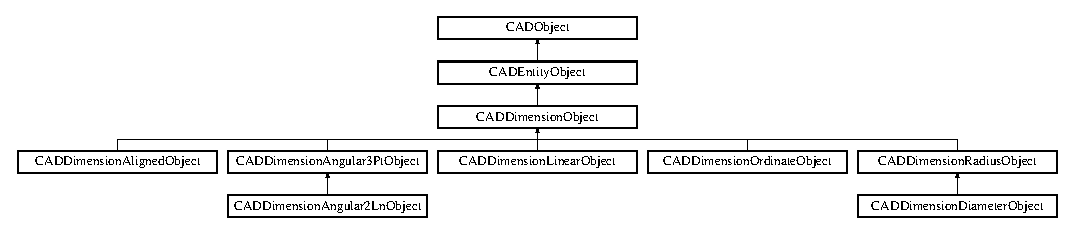
\includegraphics[height=2.692308cm]{class_c_a_d_dimension_object}
\end{center}
\end{figure}
\subsection*{Public Attributes}
\begin{DoxyCompactItemize}
\item 
\hyperlink{struct__dimdata}{C\+A\+D\+Common\+Dimension\+Data} {\bfseries cdd}\hypertarget{class_c_a_d_dimension_object_a73ad5ed391445b6b0e18323927144e01}{}\label{class_c_a_d_dimension_object_a73ad5ed391445b6b0e18323927144e01}

\item 
\hyperlink{class_c_a_d_vector}{C\+A\+D\+Vector} {\bfseries vert10pt}\hypertarget{class_c_a_d_dimension_object_a900a32ed2795f3b61a1c5ecf26b68f24}{}\label{class_c_a_d_dimension_object_a900a32ed2795f3b61a1c5ecf26b68f24}

\item 
\hyperlink{class_c_a_d_handle}{C\+A\+D\+Handle} {\bfseries h\+Dimstyle}\hypertarget{class_c_a_d_dimension_object_a78613efb7a752bdb4168260893eceda9}{}\label{class_c_a_d_dimension_object_a78613efb7a752bdb4168260893eceda9}

\item 
\hyperlink{class_c_a_d_handle}{C\+A\+D\+Handle} {\bfseries h\+Anonymous\+Block}\hypertarget{class_c_a_d_dimension_object_a83cc9d355a3bb00a0773fc3ecd35a6ef}{}\label{class_c_a_d_dimension_object_a83cc9d355a3bb00a0773fc3ecd35a6ef}

\end{DoxyCompactItemize}
\subsection*{Additional Inherited Members}


\subsection{Detailed Description}
The \hyperlink{class_c_a_d_dimension_object}{C\+A\+D\+Dimension\+Object} class. 

The documentation for this class was generated from the following file\+:\begin{DoxyCompactItemize}
\item 
cadobjects.\+h\end{DoxyCompactItemize}

\hypertarget{class_c_a_d_dimension_ordinate_object}{}\section{C\+A\+D\+Dimension\+Ordinate\+Object Class Reference}
\label{class_c_a_d_dimension_ordinate_object}\index{C\+A\+D\+Dimension\+Ordinate\+Object@{C\+A\+D\+Dimension\+Ordinate\+Object}}


The \hyperlink{class_c_a_d_dimension_ordinate_object}{C\+A\+D\+Dimension\+Ordinate\+Object} class.  




{\ttfamily \#include $<$cadobjects.\+h$>$}

Inheritance diagram for C\+A\+D\+Dimension\+Ordinate\+Object\+:\begin{figure}[H]
\begin{center}
\leavevmode
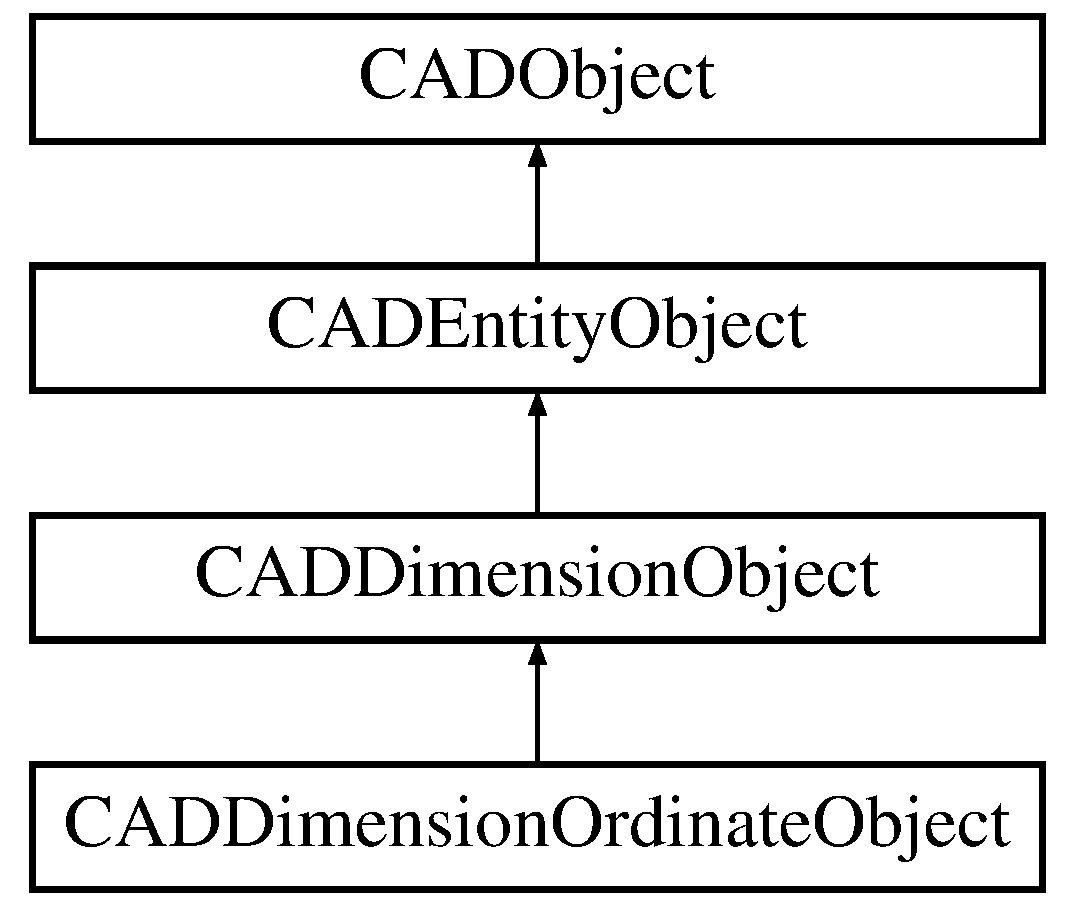
\includegraphics[height=4.000000cm]{class_c_a_d_dimension_ordinate_object}
\end{center}
\end{figure}
\subsection*{Public Attributes}
\begin{DoxyCompactItemize}
\item 
\hyperlink{class_c_a_d_vector}{C\+A\+D\+Vector} {\bfseries vert13pt}\hypertarget{class_c_a_d_dimension_ordinate_object_aa3029046f411076a3e50f92b5c958c9b}{}\label{class_c_a_d_dimension_ordinate_object_aa3029046f411076a3e50f92b5c958c9b}

\item 
\hyperlink{class_c_a_d_vector}{C\+A\+D\+Vector} {\bfseries vert14pt}\hypertarget{class_c_a_d_dimension_ordinate_object_af6eef204a20ec4a6bbc5b9eb54a01659}{}\label{class_c_a_d_dimension_ordinate_object_af6eef204a20ec4a6bbc5b9eb54a01659}

\item 
unsigned char {\bfseries Flags2}\hypertarget{class_c_a_d_dimension_ordinate_object_a8b66bf4d3cd7ae8e51a15e9115519cbe}{}\label{class_c_a_d_dimension_ordinate_object_a8b66bf4d3cd7ae8e51a15e9115519cbe}

\end{DoxyCompactItemize}
\subsection*{Additional Inherited Members}


\subsection{Detailed Description}
The \hyperlink{class_c_a_d_dimension_ordinate_object}{C\+A\+D\+Dimension\+Ordinate\+Object} class. 

The documentation for this class was generated from the following files\+:\begin{DoxyCompactItemize}
\item 
cadobjects.\+h\item 
cadobjects.\+cpp\end{DoxyCompactItemize}

\hypertarget{class_c_a_d_dimension_radius_object}{}\section{C\+A\+D\+Dimension\+Radius\+Object Class Reference}
\label{class_c_a_d_dimension_radius_object}\index{C\+A\+D\+Dimension\+Radius\+Object@{C\+A\+D\+Dimension\+Radius\+Object}}


The \hyperlink{class_c_a_d_dimension_radius_object}{C\+A\+D\+Dimension\+Radius\+Object} class.  




{\ttfamily \#include $<$cadobjects.\+h$>$}

Inheritance diagram for C\+A\+D\+Dimension\+Radius\+Object\+:\begin{figure}[H]
\begin{center}
\leavevmode
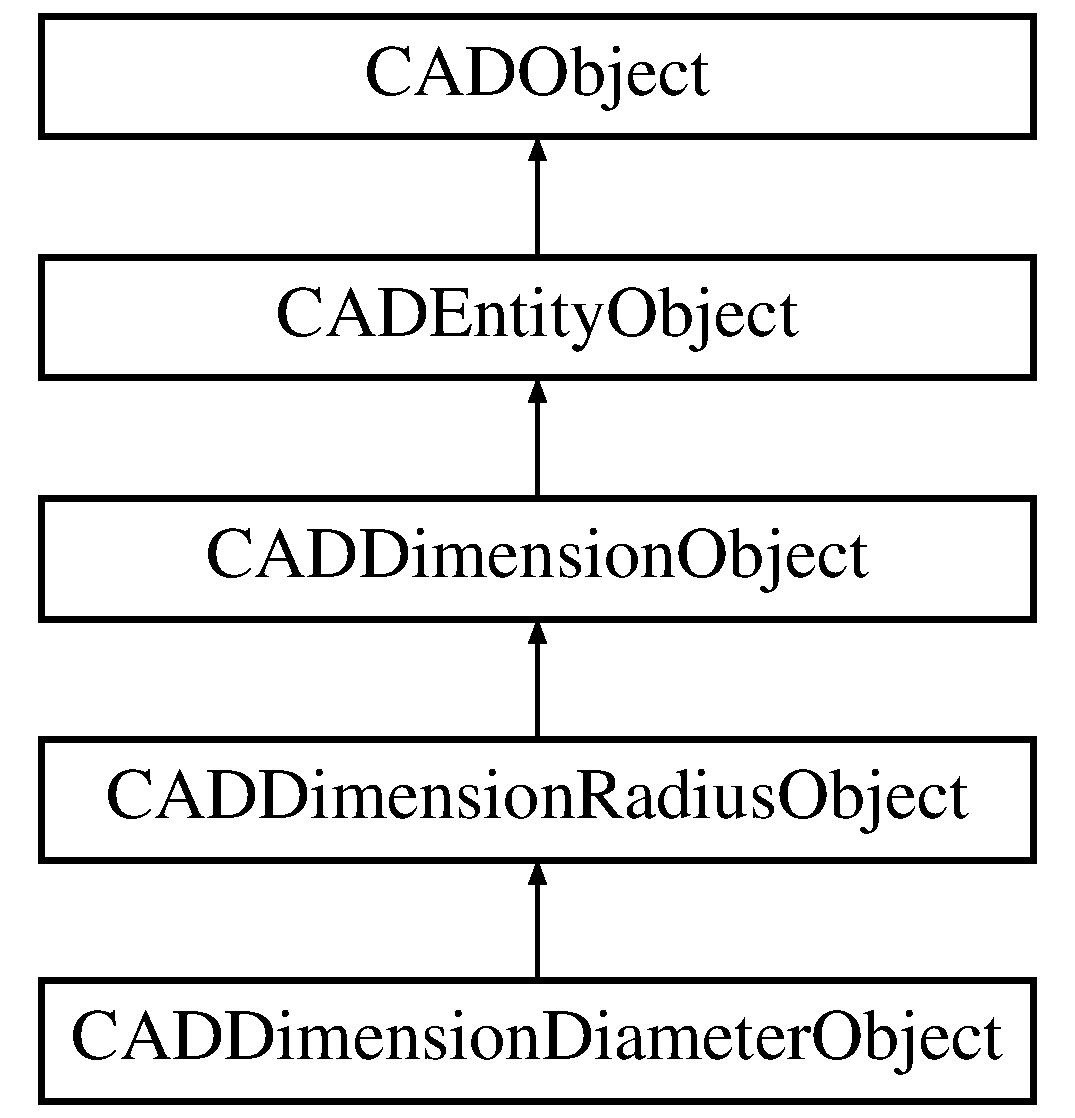
\includegraphics[height=5.000000cm]{class_c_a_d_dimension_radius_object}
\end{center}
\end{figure}
\subsection*{Public Attributes}
\begin{DoxyCompactItemize}
\item 
\hyperlink{class_c_a_d_vector}{C\+A\+D\+Vector} {\bfseries vert15pt}\hypertarget{class_c_a_d_dimension_radius_object_a24c3c5ec18527cbb03ea38ea227d6ef0}{}\label{class_c_a_d_dimension_radius_object_a24c3c5ec18527cbb03ea38ea227d6ef0}

\item 
double {\bfseries df\+Leader\+Len}\hypertarget{class_c_a_d_dimension_radius_object_aeca09b0c2899e1e4c15e69b4262227e7}{}\label{class_c_a_d_dimension_radius_object_aeca09b0c2899e1e4c15e69b4262227e7}

\end{DoxyCompactItemize}
\subsection*{Additional Inherited Members}


\subsection{Detailed Description}
The \hyperlink{class_c_a_d_dimension_radius_object}{C\+A\+D\+Dimension\+Radius\+Object} class. 

The documentation for this class was generated from the following files\+:\begin{DoxyCompactItemize}
\item 
cadobjects.\+h\item 
cadobjects.\+cpp\end{DoxyCompactItemize}

\hypertarget{class_c_a_d_ellipse}{}\section{C\+A\+D\+Ellipse Class Reference}
\label{class_c_a_d_ellipse}\index{C\+A\+D\+Ellipse@{C\+A\+D\+Ellipse}}


Geometry class which represents Ellipse.  




{\ttfamily \#include $<$cadgeometry.\+h$>$}

Inheritance diagram for C\+A\+D\+Ellipse\+:\begin{figure}[H]
\begin{center}
\leavevmode
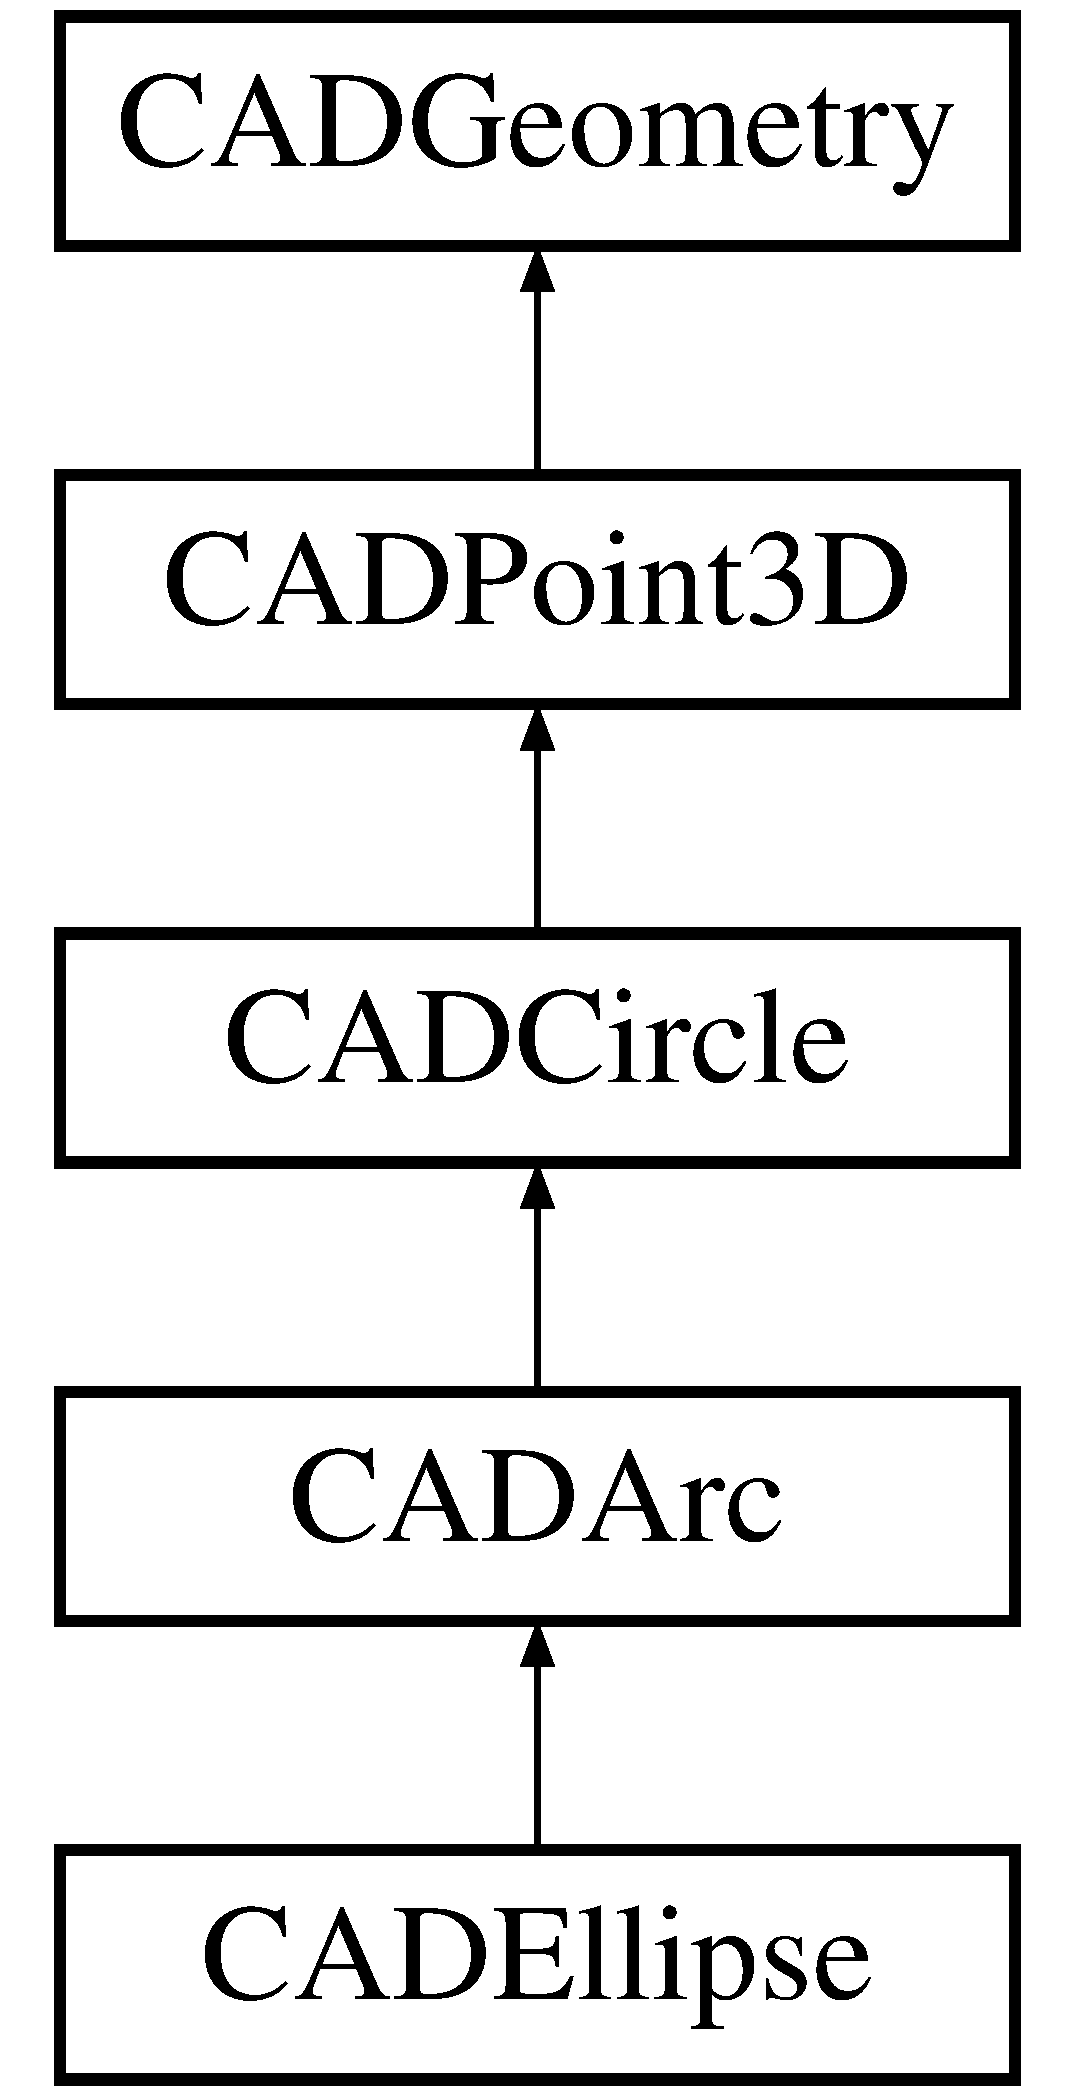
\includegraphics[height=5.000000cm]{class_c_a_d_ellipse}
\end{center}
\end{figure}
\subsection*{Public Member Functions}
\begin{DoxyCompactItemize}
\item 
double {\bfseries get\+Axis\+Ratio} () const \hypertarget{class_c_a_d_ellipse_a54e9ced7ab524253326a0f6379ef5a3a}{}\label{class_c_a_d_ellipse_a54e9ced7ab524253326a0f6379ef5a3a}

\item 
void {\bfseries set\+Axis\+Ratio} (double value)\hypertarget{class_c_a_d_ellipse_ac49d3acec034fa23cb51b51f9c454305}{}\label{class_c_a_d_ellipse_ac49d3acec034fa23cb51b51f9c454305}

\item 
virtual void {\bfseries print} () const  override\hypertarget{class_c_a_d_ellipse_a2b8f06c7da2cde09a252754d515a5be2}{}\label{class_c_a_d_ellipse_a2b8f06c7da2cde09a252754d515a5be2}

\end{DoxyCompactItemize}
\subsection*{Protected Attributes}
\begin{DoxyCompactItemize}
\item 
double {\bfseries axis\+Ratio}\hypertarget{class_c_a_d_ellipse_a058d2582f555840c258e2a93e15843de}{}\label{class_c_a_d_ellipse_a058d2582f555840c258e2a93e15843de}

\end{DoxyCompactItemize}
\subsection*{Additional Inherited Members}


\subsection{Detailed Description}
Geometry class which represents Ellipse. 

The documentation for this class was generated from the following files\+:\begin{DoxyCompactItemize}
\item 
cadgeometry.\+h\item 
cadgeometry.\+cpp\end{DoxyCompactItemize}

\hypertarget{class_c_a_d_ellipse_object}{}\section{C\+A\+D\+Ellipse\+Object Class Reference}
\label{class_c_a_d_ellipse_object}\index{C\+A\+D\+Ellipse\+Object@{C\+A\+D\+Ellipse\+Object}}


The \hyperlink{class_c_a_d_ellipse_object}{C\+A\+D\+Ellipse\+Object} class.  




{\ttfamily \#include $<$cadobjects.\+h$>$}

Inheritance diagram for C\+A\+D\+Ellipse\+Object\+:\begin{figure}[H]
\begin{center}
\leavevmode
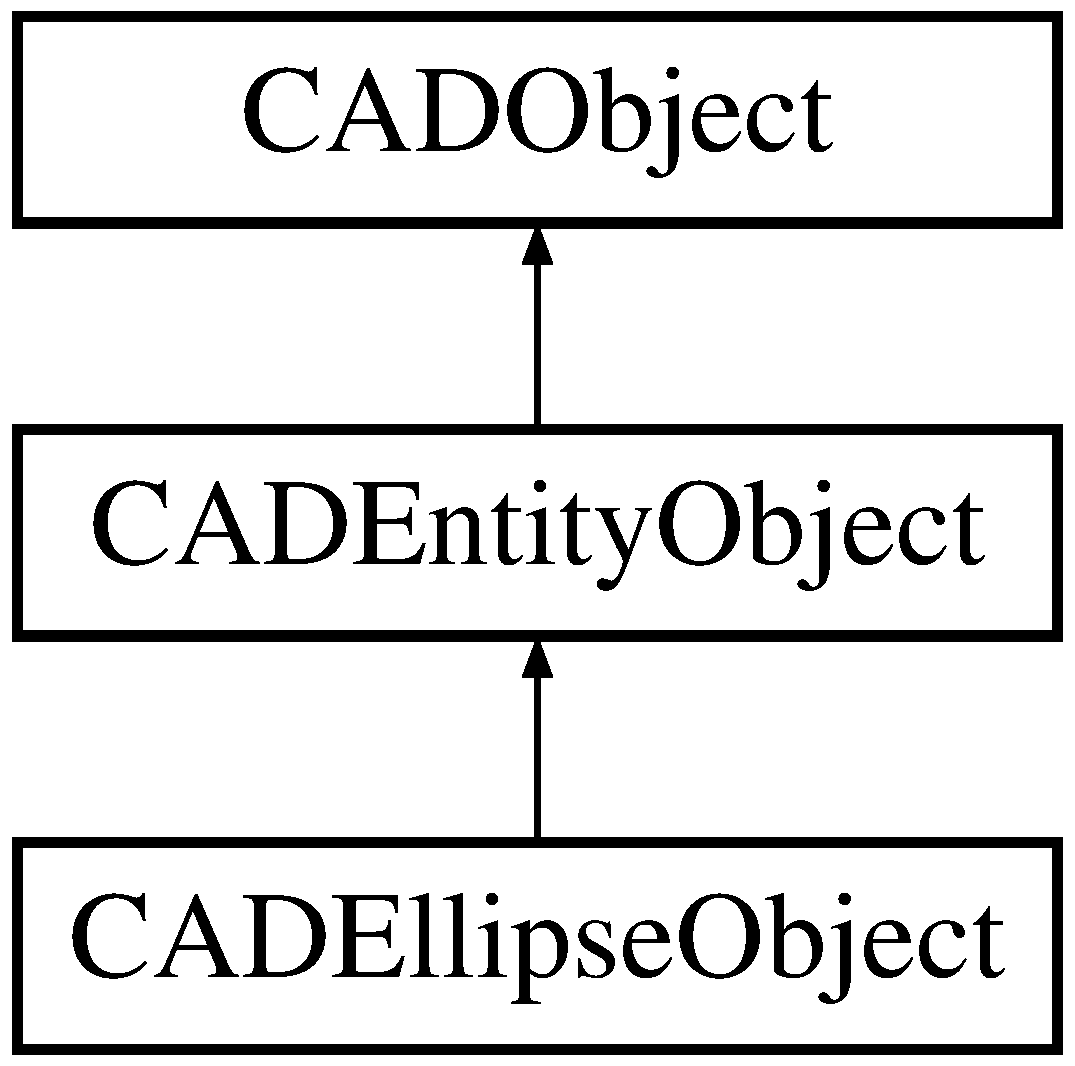
\includegraphics[height=3.000000cm]{class_c_a_d_ellipse_object}
\end{center}
\end{figure}
\subsection*{Public Attributes}
\begin{DoxyCompactItemize}
\item 
\hyperlink{class_c_a_d_vector}{C\+A\+D\+Vector} {\bfseries vert\+Position}\hypertarget{class_c_a_d_ellipse_object_a5deae79d992672502a800e4fe7a1f03c}{}\label{class_c_a_d_ellipse_object_a5deae79d992672502a800e4fe7a1f03c}

\item 
\hyperlink{class_c_a_d_vector}{C\+A\+D\+Vector} {\bfseries vect\+S\+M\+Axis}\hypertarget{class_c_a_d_ellipse_object_a2526b4a1eeaeb93b42eb54c3dcf99a67}{}\label{class_c_a_d_ellipse_object_a2526b4a1eeaeb93b42eb54c3dcf99a67}

\item 
\hyperlink{class_c_a_d_vector}{C\+A\+D\+Vector} {\bfseries vect\+Extrusion}\hypertarget{class_c_a_d_ellipse_object_a9570d612f5e53a182cc58742f4d1d98a}{}\label{class_c_a_d_ellipse_object_a9570d612f5e53a182cc58742f4d1d98a}

\item 
double {\bfseries df\+Axis\+Ratio}\hypertarget{class_c_a_d_ellipse_object_ae6eb44bdcddb79622a25efb231aca2c3}{}\label{class_c_a_d_ellipse_object_ae6eb44bdcddb79622a25efb231aca2c3}

\item 
double {\bfseries df\+Beg\+Angle}\hypertarget{class_c_a_d_ellipse_object_a28219caecc8b5f7acb29f4a09613991e}{}\label{class_c_a_d_ellipse_object_a28219caecc8b5f7acb29f4a09613991e}

\item 
double {\bfseries df\+End\+Angle}\hypertarget{class_c_a_d_ellipse_object_aa87ce711d75f6681e980e2e52a6b7573}{}\label{class_c_a_d_ellipse_object_aa87ce711d75f6681e980e2e52a6b7573}

\end{DoxyCompactItemize}
\subsection*{Additional Inherited Members}


\subsection{Detailed Description}
The \hyperlink{class_c_a_d_ellipse_object}{C\+A\+D\+Ellipse\+Object} class. 

The documentation for this class was generated from the following files\+:\begin{DoxyCompactItemize}
\item 
cadobjects.\+h\item 
cadobjects.\+cpp\end{DoxyCompactItemize}

\hypertarget{class_c_a_d_endblk_object}{}\section{C\+A\+D\+Endblk\+Object Class Reference}
\label{class_c_a_d_endblk_object}\index{C\+A\+D\+Endblk\+Object@{C\+A\+D\+Endblk\+Object}}


The C\+AD End block Object class.  




{\ttfamily \#include $<$cadobjects.\+h$>$}

Inheritance diagram for C\+A\+D\+Endblk\+Object\+:\begin{figure}[H]
\begin{center}
\leavevmode
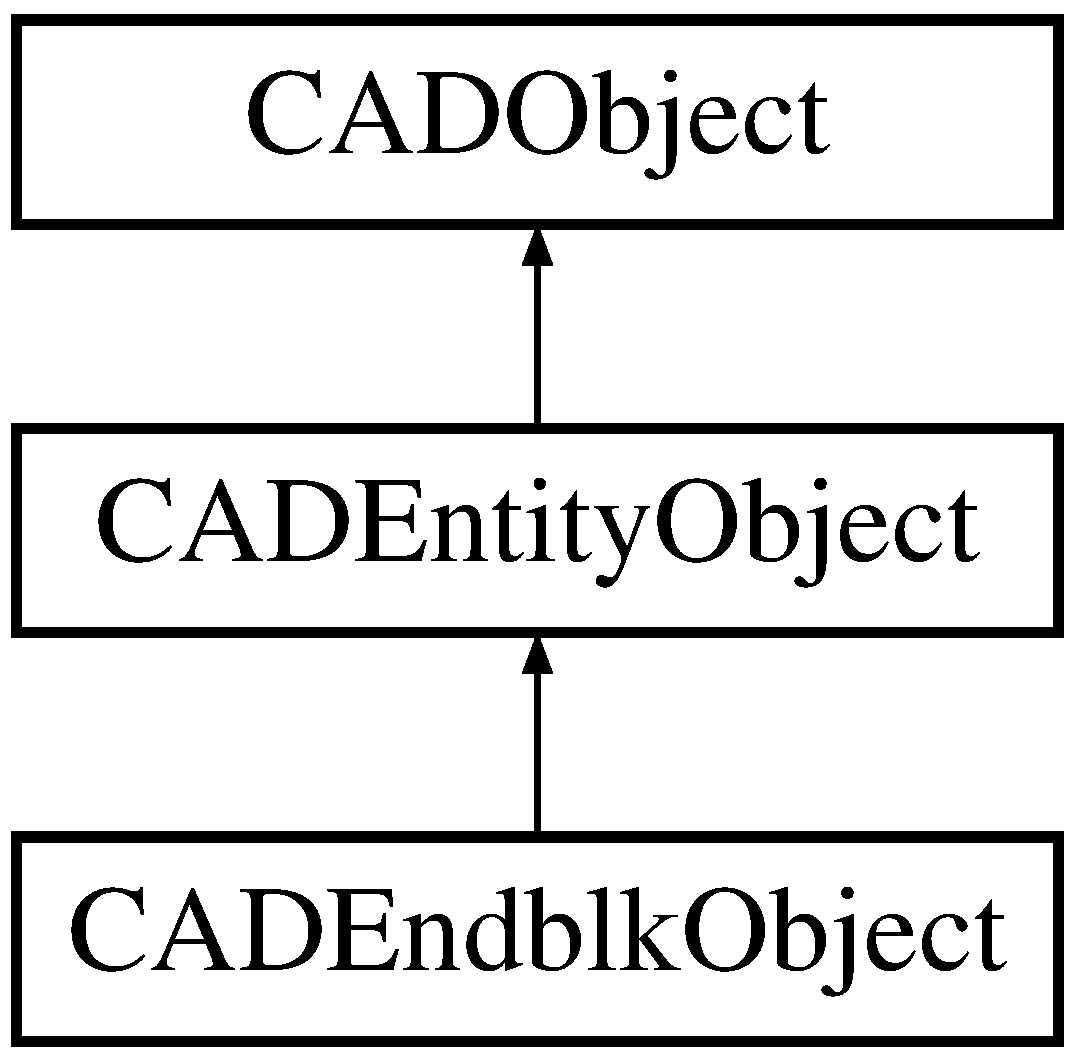
\includegraphics[height=3.000000cm]{class_c_a_d_endblk_object}
\end{center}
\end{figure}
\subsection*{Additional Inherited Members}


\subsection{Detailed Description}
The C\+AD End block Object class. 

The documentation for this class was generated from the following files\+:\begin{DoxyCompactItemize}
\item 
cadobjects.\+h\item 
cadobjects.\+cpp\end{DoxyCompactItemize}

\hypertarget{class_c_a_d_entity_object}{}\section{C\+A\+D\+Entity\+Object Class Reference}
\label{class_c_a_d_entity_object}\index{C\+A\+D\+Entity\+Object@{C\+A\+D\+Entity\+Object}}
Inheritance diagram for C\+A\+D\+Entity\+Object\+:\begin{figure}[H]
\begin{center}
\leavevmode
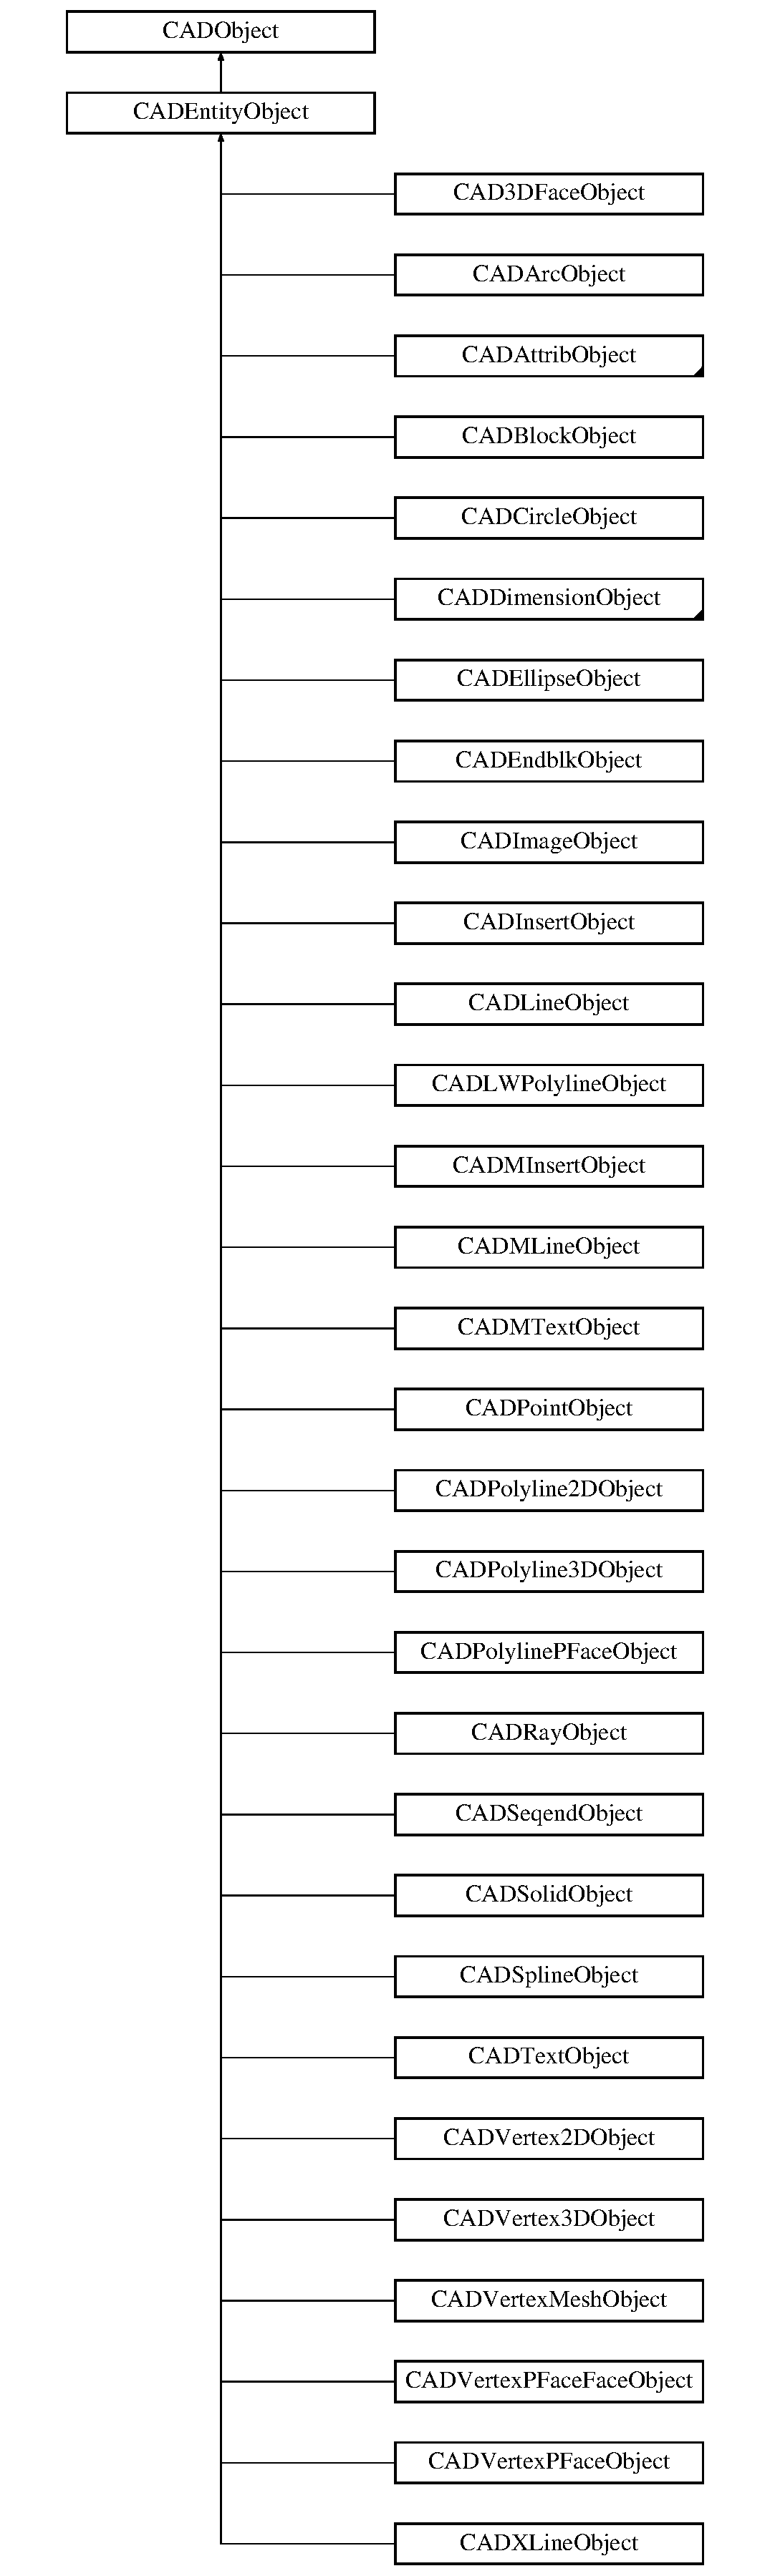
\includegraphics[height=12.000000cm]{class_c_a_d_entity_object}
\end{center}
\end{figure}
\subsection*{Public Attributes}
\begin{DoxyCompactItemize}
\item 
struct \hyperlink{struct_c_a_d_common_e_d}{C\+A\+D\+Common\+ED} {\bfseries st\+Ced}\hypertarget{class_c_a_d_entity_object_a66c5148109d5008278079b2c9d4e10b5}{}\label{class_c_a_d_entity_object_a66c5148109d5008278079b2c9d4e10b5}

\item 
struct \hyperlink{struct_c_a_d_common_e_h_d}{C\+A\+D\+Common\+E\+HD} {\bfseries st\+Ched}\hypertarget{class_c_a_d_entity_object_a9511816e79ca3c030f28e0ea91bc36fa}{}\label{class_c_a_d_entity_object_a9511816e79ca3c030f28e0ea91bc36fa}

\end{DoxyCompactItemize}
\subsection*{Additional Inherited Members}


The documentation for this class was generated from the following file\+:\begin{DoxyCompactItemize}
\item 
cadobjects.\+h\end{DoxyCompactItemize}

\hypertarget{class_c_a_d_face3_d}{}\section{C\+A\+D\+Face3D Class Reference}
\label{class_c_a_d_face3_d}\index{C\+A\+D\+Face3D@{C\+A\+D\+Face3D}}


Geometry class which represents 3\+D\+Face.  




{\ttfamily \#include $<$cadgeometry.\+h$>$}

Inheritance diagram for C\+A\+D\+Face3D\+:\begin{figure}[H]
\begin{center}
\leavevmode
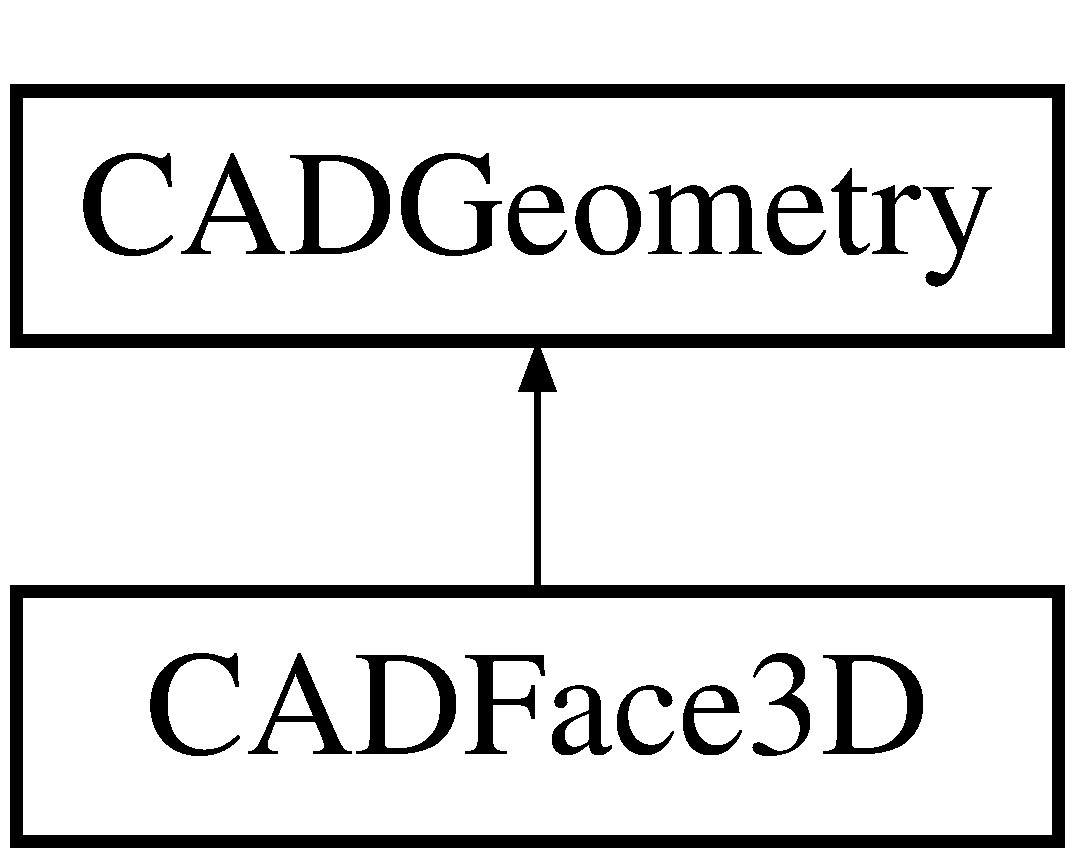
\includegraphics[height=2.000000cm]{class_c_a_d_face3_d}
\end{center}
\end{figure}
\subsection*{Public Member Functions}
\begin{DoxyCompactItemize}
\item 
void {\bfseries add\+Corner} (const \hyperlink{class_c_a_d_vector}{C\+A\+D\+Vector} \&corner)\hypertarget{class_c_a_d_face3_d_aa173b3c57c8e5d223185f50a30b24d5c}{}\label{class_c_a_d_face3_d_aa173b3c57c8e5d223185f50a30b24d5c}

\item 
virtual void {\bfseries print} () const  override\hypertarget{class_c_a_d_face3_d_ae7d28d2b9934dd233f262ed7498a56de}{}\label{class_c_a_d_face3_d_ae7d28d2b9934dd233f262ed7498a56de}

\item 
short {\bfseries get\+Invis\+Flags} () const \hypertarget{class_c_a_d_face3_d_a9d9bac1cf36a63993e185de8efbe034c}{}\label{class_c_a_d_face3_d_a9d9bac1cf36a63993e185de8efbe034c}

\item 
void {\bfseries set\+Invis\+Flags} (short value)\hypertarget{class_c_a_d_face3_d_a8dd54f639fc34e38cfba6c8688905523}{}\label{class_c_a_d_face3_d_a8dd54f639fc34e38cfba6c8688905523}

\end{DoxyCompactItemize}
\subsection*{Protected Attributes}
\begin{DoxyCompactItemize}
\item 
vector$<$ \hyperlink{class_c_a_d_vector}{C\+A\+D\+Vector} $>$ {\bfseries avert\+Corners}\hypertarget{class_c_a_d_face3_d_a4e72cf3fd2cfda9470bd1d67b6b5c8b9}{}\label{class_c_a_d_face3_d_a4e72cf3fd2cfda9470bd1d67b6b5c8b9}

\item 
short {\bfseries invis\+Flags}\hypertarget{class_c_a_d_face3_d_a64f7f3115db8442d07a5da218e693654}{}\label{class_c_a_d_face3_d_a64f7f3115db8442d07a5da218e693654}

\end{DoxyCompactItemize}
\subsection*{Additional Inherited Members}


\subsection{Detailed Description}
Geometry class which represents 3\+D\+Face. 

The documentation for this class was generated from the following files\+:\begin{DoxyCompactItemize}
\item 
cadgeometry.\+h\item 
cadgeometry.\+cpp\end{DoxyCompactItemize}

\hypertarget{class_c_a_d_file}{}\section{C\+A\+D\+File Class Reference}
\label{class_c_a_d_file}\index{C\+A\+D\+File@{C\+A\+D\+File}}


The abstact C\+AD file class.  




{\ttfamily \#include $<$cadfile.\+h$>$}

Inheritance diagram for C\+A\+D\+File\+:\begin{figure}[H]
\begin{center}
\leavevmode
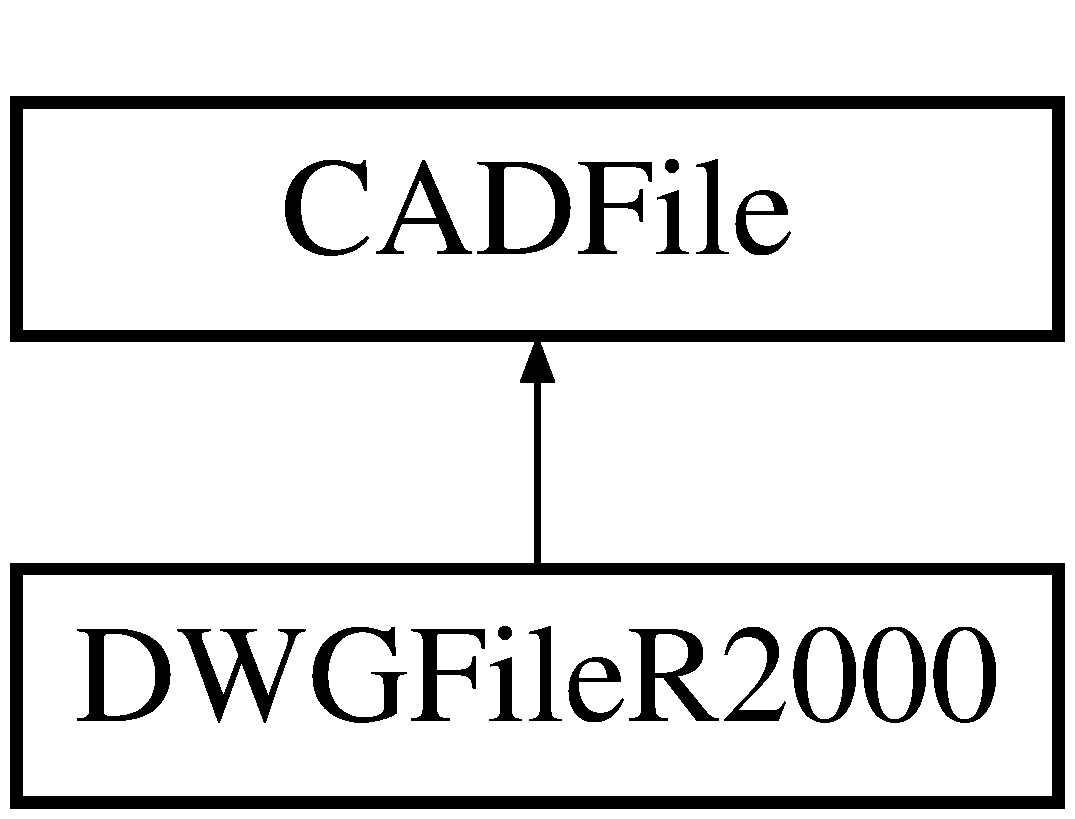
\includegraphics[height=2.000000cm]{class_c_a_d_file}
\end{center}
\end{figure}
\subsection*{Public Types}
\begin{DoxyCompactItemize}
\item 
enum \hyperlink{class_c_a_d_file_a4776c7f9fc5888cac0ee6eede900db5a}{Open\+Options} \{ \hyperlink{class_c_a_d_file_a4776c7f9fc5888cac0ee6eede900db5aa31951f81322352b41b9969dfa90e8239}{R\+E\+A\+D\+\_\+\+A\+LL}, 
\hyperlink{class_c_a_d_file_a4776c7f9fc5888cac0ee6eede900db5aab28ae38caf2847fb4895de25acf5cbe7}{R\+E\+A\+D\+\_\+\+F\+A\+ST}, 
\hyperlink{class_c_a_d_file_a4776c7f9fc5888cac0ee6eede900db5aa0a071ae71397d2dcf724cf627e62ec65}{R\+E\+A\+D\+\_\+\+F\+A\+S\+T\+E\+ST}
 \}\begin{DoxyCompactList}\small\item\em The C\+AD file open options enum. \end{DoxyCompactList}
\end{DoxyCompactItemize}
\subsection*{Public Member Functions}
\begin{DoxyCompactItemize}
\item 
{\bfseries C\+A\+D\+File} (\hyperlink{class_c_a_d_file_i_o}{C\+A\+D\+File\+IO} $\ast$po\+File\+IO)\hypertarget{class_c_a_d_file_a29cf9e51220c9bd2242067f065fefa12}{}\label{class_c_a_d_file_a29cf9e51220c9bd2242067f065fefa12}

\item 
const \hyperlink{class_c_a_d_header}{C\+A\+D\+Header} \& {\bfseries get\+Header} () const \hypertarget{class_c_a_d_file_a7fd02ff6859073889ddc1f48ef231fb5}{}\label{class_c_a_d_file_a7fd02ff6859073889ddc1f48ef231fb5}

\item 
const \hyperlink{class_c_a_d_classes}{C\+A\+D\+Classes} \& {\bfseries get\+Classes} () const \hypertarget{class_c_a_d_file_a38f0e7d2f11f31be149a1d6f67e1dac7}{}\label{class_c_a_d_file_a38f0e7d2f11f31be149a1d6f67e1dac7}

\item 
const \hyperlink{class_c_a_d_tables}{C\+A\+D\+Tables} \& {\bfseries get\+Tables} () const \hypertarget{class_c_a_d_file_a950a209c6a096013fd7bdb61d22764d3}{}\label{class_c_a_d_file_a950a209c6a096013fd7bdb61d22764d3}

\item 
virtual int {\bfseries parse\+File} (enum \hyperlink{class_c_a_d_file_a4776c7f9fc5888cac0ee6eede900db5a}{Open\+Options} e\+Options)\hypertarget{class_c_a_d_file_a591e193ee4fceda0f48811ca9e94858d}{}\label{class_c_a_d_file_a591e193ee4fceda0f48811ca9e94858d}

\item 
virtual size\+\_\+t {\bfseries get\+Layers\+Count} () const \hypertarget{class_c_a_d_file_a68b5053784e3ea7956abec99ed51727d}{}\label{class_c_a_d_file_a68b5053784e3ea7956abec99ed51727d}

\item 
virtual \hyperlink{class_c_a_d_layer}{C\+A\+D\+Layer} \& {\bfseries get\+Layer} (size\+\_\+t index)\hypertarget{class_c_a_d_file_a44f461c84fcd6afb4e9a3e76815a0e31}{}\label{class_c_a_d_file_a44f461c84fcd6afb4e9a3e76815a0e31}

\end{DoxyCompactItemize}
\subsection*{Protected Member Functions}
\begin{DoxyCompactItemize}
\item 
virtual \hyperlink{class_c_a_d_object}{C\+A\+D\+Object} $\ast$ \hyperlink{class_c_a_d_file_aeb68cd431afb9c5657ae7cbe06deffc6}{get\+Object} (long index)=0
\begin{DoxyCompactList}\small\item\em Get C\+AD Object from file. \end{DoxyCompactList}\item 
virtual \hyperlink{class_c_a_d_geometry}{C\+A\+D\+Geometry} $\ast$ \hyperlink{class_c_a_d_file_a1c841beaf00d33fe888d5f750841829b}{get\+Geometry} (long index)=0
\begin{DoxyCompactList}\small\item\em read geometry from C\+AD file \end{DoxyCompactList}\item 
virtual int \hyperlink{class_c_a_d_file_a160199a6f2004ea5ed319639e2f1156e}{read\+Section\+Locator} ()=0
\begin{DoxyCompactList}\small\item\em initially read some basic values and section locator \end{DoxyCompactList}\item 
virtual int \hyperlink{class_c_a_d_file_a27a0eed4be75e5e1fcc9ca8ba9f881c8}{read\+Header} (enum \hyperlink{class_c_a_d_file_a4776c7f9fc5888cac0ee6eede900db5a}{Open\+Options} e\+Options)=0
\begin{DoxyCompactList}\small\item\em Read header from C\+AD file. \end{DoxyCompactList}\item 
virtual int \hyperlink{class_c_a_d_file_a3965f0e1668a25ce2ed06c9e8e1bffdd}{read\+Classes} (enum \hyperlink{class_c_a_d_file_a4776c7f9fc5888cac0ee6eede900db5a}{Open\+Options} e\+Options)=0
\begin{DoxyCompactList}\small\item\em Read classes from C\+AD file. \end{DoxyCompactList}\item 
virtual int \hyperlink{class_c_a_d_file_aac33914479442df31a4ab45df8e9e8a3}{create\+File\+Map} ()=0
\begin{DoxyCompactList}\small\item\em Create the file map for fast access to C\+AD objects. \end{DoxyCompactList}\item 
virtual int \hyperlink{class_c_a_d_file_a3e1d2a8827b5af6ba0ead4b746215eb7}{read\+Tables} (enum \hyperlink{class_c_a_d_file_a4776c7f9fc5888cac0ee6eede900db5a}{Open\+Options} e\+Options)
\begin{DoxyCompactList}\small\item\em Read tables from C\+AD file. \end{DoxyCompactList}\end{DoxyCompactItemize}
\subsection*{Protected Attributes}
\begin{DoxyCompactItemize}
\item 
\hyperlink{class_c_a_d_file_i_o}{C\+A\+D\+File\+IO} $\ast$ {\bfseries file\+IO}\hypertarget{class_c_a_d_file_a520638860613882f28d871a2b3144e4d}{}\label{class_c_a_d_file_a520638860613882f28d871a2b3144e4d}

\item 
\hyperlink{class_c_a_d_header}{C\+A\+D\+Header} {\bfseries header}\hypertarget{class_c_a_d_file_ac4d7214d67374a266f763c87a9aed14c}{}\label{class_c_a_d_file_ac4d7214d67374a266f763c87a9aed14c}

\item 
\hyperlink{class_c_a_d_classes}{C\+A\+D\+Classes} {\bfseries classes}\hypertarget{class_c_a_d_file_a7b2a7683e84744800db66aba4892ec8e}{}\label{class_c_a_d_file_a7b2a7683e84744800db66aba4892ec8e}

\item 
\hyperlink{class_c_a_d_tables}{C\+A\+D\+Tables} {\bfseries tables}\hypertarget{class_c_a_d_file_afada89607a282b33061b63d9f67ac89c}{}\label{class_c_a_d_file_afada89607a282b33061b63d9f67ac89c}

\item 
std\+::map$<$ long, long $>$ {\bfseries objects\+Map}\hypertarget{class_c_a_d_file_a83d212922cd2e95466c0aad6ae3a746f}{}\label{class_c_a_d_file_a83d212922cd2e95466c0aad6ae3a746f}

\end{DoxyCompactItemize}
\subsection*{Friends}
\begin{DoxyCompactItemize}
\item 
class {\bfseries C\+A\+D\+Tables}\hypertarget{class_c_a_d_file_abbe0590d91a084db4f9d96a24868b3a0}{}\label{class_c_a_d_file_abbe0590d91a084db4f9d96a24868b3a0}

\item 
class {\bfseries C\+A\+D\+Layer}\hypertarget{class_c_a_d_file_aa43e75f3b7c4e30bf22233f08cc9f31b}{}\label{class_c_a_d_file_aa43e75f3b7c4e30bf22233f08cc9f31b}

\end{DoxyCompactItemize}


\subsection{Detailed Description}
The abstact C\+AD file class. 

\subsection{Member Enumeration Documentation}
\index{C\+A\+D\+File@{C\+A\+D\+File}!Open\+Options@{Open\+Options}}
\index{Open\+Options@{Open\+Options}!C\+A\+D\+File@{C\+A\+D\+File}}
\subsubsection[{\texorpdfstring{Open\+Options}{OpenOptions}}]{\setlength{\rightskip}{0pt plus 5cm}enum {\bf C\+A\+D\+File\+::\+Open\+Options}}\hypertarget{class_c_a_d_file_a4776c7f9fc5888cac0ee6eede900db5a}{}\label{class_c_a_d_file_a4776c7f9fc5888cac0ee6eede900db5a}


The C\+AD file open options enum. 

\begin{Desc}
\item[Enumerator]\par
\begin{description}
\index{R\+E\+A\+D\+\_\+\+A\+LL@{R\+E\+A\+D\+\_\+\+A\+LL}!C\+A\+D\+File@{C\+A\+D\+File}}\index{C\+A\+D\+File@{C\+A\+D\+File}!R\+E\+A\+D\+\_\+\+A\+LL@{R\+E\+A\+D\+\_\+\+A\+LL}}\item[{\em 
R\+E\+A\+D\+\_\+\+A\+LL\hypertarget{class_c_a_d_file_a4776c7f9fc5888cac0ee6eede900db5aa31951f81322352b41b9969dfa90e8239}{}\label{class_c_a_d_file_a4776c7f9fc5888cac0ee6eede900db5aa31951f81322352b41b9969dfa90e8239}
}]read all available information \index{R\+E\+A\+D\+\_\+\+F\+A\+ST@{R\+E\+A\+D\+\_\+\+F\+A\+ST}!C\+A\+D\+File@{C\+A\+D\+File}}\index{C\+A\+D\+File@{C\+A\+D\+File}!R\+E\+A\+D\+\_\+\+F\+A\+ST@{R\+E\+A\+D\+\_\+\+F\+A\+ST}}\item[{\em 
R\+E\+A\+D\+\_\+\+F\+A\+ST\hypertarget{class_c_a_d_file_a4776c7f9fc5888cac0ee6eede900db5aab28ae38caf2847fb4895de25acf5cbe7}{}\label{class_c_a_d_file_a4776c7f9fc5888cac0ee6eede900db5aab28ae38caf2847fb4895de25acf5cbe7}
}]read some methadata \index{R\+E\+A\+D\+\_\+\+F\+A\+S\+T\+E\+ST@{R\+E\+A\+D\+\_\+\+F\+A\+S\+T\+E\+ST}!C\+A\+D\+File@{C\+A\+D\+File}}\index{C\+A\+D\+File@{C\+A\+D\+File}!R\+E\+A\+D\+\_\+\+F\+A\+S\+T\+E\+ST@{R\+E\+A\+D\+\_\+\+F\+A\+S\+T\+E\+ST}}\item[{\em 
R\+E\+A\+D\+\_\+\+F\+A\+S\+T\+E\+ST\hypertarget{class_c_a_d_file_a4776c7f9fc5888cac0ee6eede900db5aa0a071ae71397d2dcf724cf627e62ec65}{}\label{class_c_a_d_file_a4776c7f9fc5888cac0ee6eede900db5aa0a071ae71397d2dcf724cf627e62ec65}
}]read only geometry and layers \end{description}
\end{Desc}


\subsection{Member Function Documentation}
\index{C\+A\+D\+File@{C\+A\+D\+File}!create\+File\+Map@{create\+File\+Map}}
\index{create\+File\+Map@{create\+File\+Map}!C\+A\+D\+File@{C\+A\+D\+File}}
\subsubsection[{\texorpdfstring{create\+File\+Map()=0}{createFileMap()=0}}]{\setlength{\rightskip}{0pt plus 5cm}virtual int C\+A\+D\+File\+::create\+File\+Map (
\begin{DoxyParamCaption}
{}
\end{DoxyParamCaption}
)\hspace{0.3cm}{\ttfamily [protected]}, {\ttfamily [pure virtual]}}\hypertarget{class_c_a_d_file_aac33914479442df31a4ab45df8e9e8a3}{}\label{class_c_a_d_file_aac33914479442df31a4ab45df8e9e8a3}


Create the file map for fast access to C\+AD objects. 

\begin{DoxyReturn}{Returns}
C\+A\+D\+Error\+Codes\+::\+S\+U\+C\+C\+E\+SS if OK, or error code 
\end{DoxyReturn}


Implemented in \hyperlink{class_d_w_g_file_r2000_a8ac0c8003944b948e3d1f16c713e8e27}{D\+W\+G\+File\+R2000}.

\index{C\+A\+D\+File@{C\+A\+D\+File}!get\+Geometry@{get\+Geometry}}
\index{get\+Geometry@{get\+Geometry}!C\+A\+D\+File@{C\+A\+D\+File}}
\subsubsection[{\texorpdfstring{get\+Geometry(long index)=0}{getGeometry(long index)=0}}]{\setlength{\rightskip}{0pt plus 5cm}virtual {\bf C\+A\+D\+Geometry}$\ast$ C\+A\+D\+File\+::get\+Geometry (
\begin{DoxyParamCaption}
\item[{long}]{index}
\end{DoxyParamCaption}
)\hspace{0.3cm}{\ttfamily [protected]}, {\ttfamily [pure virtual]}}\hypertarget{class_c_a_d_file_a1c841beaf00d33fe888d5f750841829b}{}\label{class_c_a_d_file_a1c841beaf00d33fe888d5f750841829b}


read geometry from C\+AD file 


\begin{DoxyParams}{Parameters}
{\em handle} & Handle of C\+AD object \\
\hline
\end{DoxyParams}
\begin{DoxyReturn}{Returns}
N\+U\+LL if failed or pointer which mast be feed by user 
\end{DoxyReturn}


Implemented in \hyperlink{class_d_w_g_file_r2000_a8838da9ee3111f5aba1451aa59528760}{D\+W\+G\+File\+R2000}.

\index{C\+A\+D\+File@{C\+A\+D\+File}!get\+Object@{get\+Object}}
\index{get\+Object@{get\+Object}!C\+A\+D\+File@{C\+A\+D\+File}}
\subsubsection[{\texorpdfstring{get\+Object(long index)=0}{getObject(long index)=0}}]{\setlength{\rightskip}{0pt plus 5cm}virtual {\bf C\+A\+D\+Object}$\ast$ C\+A\+D\+File\+::get\+Object (
\begin{DoxyParamCaption}
\item[{long}]{index}
\end{DoxyParamCaption}
)\hspace{0.3cm}{\ttfamily [protected]}, {\ttfamily [pure virtual]}}\hypertarget{class_c_a_d_file_aeb68cd431afb9c5657ae7cbe06deffc6}{}\label{class_c_a_d_file_aeb68cd431afb9c5657ae7cbe06deffc6}


Get C\+AD Object from file. 


\begin{DoxyParams}{Parameters}
{\em index} & Object index \\
\hline
\end{DoxyParams}
\begin{DoxyReturn}{Returns}
pointer to \hyperlink{class_c_a_d_object}{C\+A\+D\+Object} or nullptr. User have to free returned pointer. 
\end{DoxyReturn}


Implemented in \hyperlink{class_d_w_g_file_r2000_a4538211a1567cff8e340d769e8a0d2c3}{D\+W\+G\+File\+R2000}.

\index{C\+A\+D\+File@{C\+A\+D\+File}!read\+Classes@{read\+Classes}}
\index{read\+Classes@{read\+Classes}!C\+A\+D\+File@{C\+A\+D\+File}}
\subsubsection[{\texorpdfstring{read\+Classes(enum Open\+Options e\+Options)=0}{readClasses(enum OpenOptions eOptions)=0}}]{\setlength{\rightskip}{0pt plus 5cm}virtual int C\+A\+D\+File\+::read\+Classes (
\begin{DoxyParamCaption}
\item[{enum {\bf Open\+Options}}]{e\+Options}
\end{DoxyParamCaption}
)\hspace{0.3cm}{\ttfamily [protected]}, {\ttfamily [pure virtual]}}\hypertarget{class_c_a_d_file_a3965f0e1668a25ce2ed06c9e8e1bffdd}{}\label{class_c_a_d_file_a3965f0e1668a25ce2ed06c9e8e1bffdd}


Read classes from C\+AD file. 


\begin{DoxyParams}{Parameters}
{\em e\+Options} & Read options \\
\hline
\end{DoxyParams}
\begin{DoxyReturn}{Returns}
C\+A\+D\+Error\+Codes\+::\+S\+U\+C\+C\+E\+SS if OK, or error code 
\end{DoxyReturn}


Implemented in \hyperlink{class_d_w_g_file_r2000_a9c0571cdd77cbc3c67612ebf8cabeccb}{D\+W\+G\+File\+R2000}.

\index{C\+A\+D\+File@{C\+A\+D\+File}!read\+Header@{read\+Header}}
\index{read\+Header@{read\+Header}!C\+A\+D\+File@{C\+A\+D\+File}}
\subsubsection[{\texorpdfstring{read\+Header(enum Open\+Options e\+Options)=0}{readHeader(enum OpenOptions eOptions)=0}}]{\setlength{\rightskip}{0pt plus 5cm}virtual int C\+A\+D\+File\+::read\+Header (
\begin{DoxyParamCaption}
\item[{enum {\bf Open\+Options}}]{e\+Options}
\end{DoxyParamCaption}
)\hspace{0.3cm}{\ttfamily [protected]}, {\ttfamily [pure virtual]}}\hypertarget{class_c_a_d_file_a27a0eed4be75e5e1fcc9ca8ba9f881c8}{}\label{class_c_a_d_file_a27a0eed4be75e5e1fcc9ca8ba9f881c8}


Read header from C\+AD file. 


\begin{DoxyParams}{Parameters}
{\em e\+Options} & Read options \\
\hline
\end{DoxyParams}
\begin{DoxyReturn}{Returns}
C\+A\+D\+Error\+Codes\+::\+S\+U\+C\+C\+E\+SS if OK, or error code 
\end{DoxyReturn}


Implemented in \hyperlink{class_d_w_g_file_r2000_a6ffef545cd473a1f2a2639f2941e4946}{D\+W\+G\+File\+R2000}.

\index{C\+A\+D\+File@{C\+A\+D\+File}!read\+Section\+Locator@{read\+Section\+Locator}}
\index{read\+Section\+Locator@{read\+Section\+Locator}!C\+A\+D\+File@{C\+A\+D\+File}}
\subsubsection[{\texorpdfstring{read\+Section\+Locator()=0}{readSectionLocator()=0}}]{\setlength{\rightskip}{0pt plus 5cm}virtual int C\+A\+D\+File\+::read\+Section\+Locator (
\begin{DoxyParamCaption}
{}
\end{DoxyParamCaption}
)\hspace{0.3cm}{\ttfamily [protected]}, {\ttfamily [pure virtual]}}\hypertarget{class_c_a_d_file_a160199a6f2004ea5ed319639e2f1156e}{}\label{class_c_a_d_file_a160199a6f2004ea5ed319639e2f1156e}


initially read some basic values and section locator 

\begin{DoxyReturn}{Returns}
C\+A\+D\+Error\+Codes\+::\+S\+U\+C\+C\+E\+SS if OK, or error code 
\end{DoxyReturn}


Implemented in \hyperlink{class_d_w_g_file_r2000_ab7e07561e251678368ffecdf6bcedf06}{D\+W\+G\+File\+R2000}.

\index{C\+A\+D\+File@{C\+A\+D\+File}!read\+Tables@{read\+Tables}}
\index{read\+Tables@{read\+Tables}!C\+A\+D\+File@{C\+A\+D\+File}}
\subsubsection[{\texorpdfstring{read\+Tables(enum Open\+Options e\+Options)}{readTables(enum OpenOptions eOptions)}}]{\setlength{\rightskip}{0pt plus 5cm}int C\+A\+D\+File\+::read\+Tables (
\begin{DoxyParamCaption}
\item[{enum {\bf Open\+Options}}]{e\+Options}
\end{DoxyParamCaption}
)\hspace{0.3cm}{\ttfamily [protected]}, {\ttfamily [virtual]}}\hypertarget{class_c_a_d_file_a3e1d2a8827b5af6ba0ead4b746215eb7}{}\label{class_c_a_d_file_a3e1d2a8827b5af6ba0ead4b746215eb7}


Read tables from C\+AD file. 


\begin{DoxyParams}{Parameters}
{\em e\+Options} & Read options \\
\hline
\end{DoxyParams}
\begin{DoxyReturn}{Returns}
C\+A\+D\+Error\+Codes\+::\+S\+U\+C\+C\+E\+SS if OK, or error code 
\end{DoxyReturn}


The documentation for this class was generated from the following files\+:\begin{DoxyCompactItemize}
\item 
cadfile.\+h\item 
cadfile.\+cpp\end{DoxyCompactItemize}

\hypertarget{class_c_a_d_file_i_o}{}\section{C\+A\+D\+File\+IO Class Reference}
\label{class_c_a_d_file_i_o}\index{C\+A\+D\+File\+IO@{C\+A\+D\+File\+IO}}


The \hyperlink{class_c_a_d_file_i_o}{C\+A\+D\+File\+IO} class provides in/out file operations as read, write, seek, etc. This is abstract class.  




{\ttfamily \#include $<$cadfileio.\+h$>$}

Inheritance diagram for C\+A\+D\+File\+IO\+:\begin{figure}[H]
\begin{center}
\leavevmode
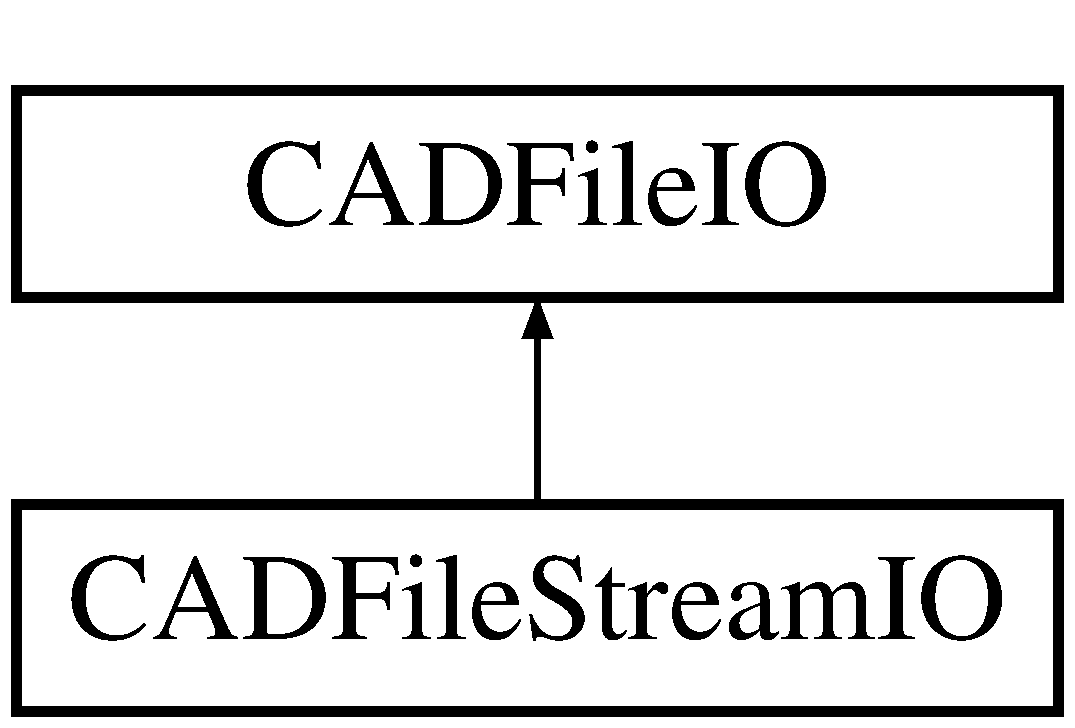
\includegraphics[height=2.000000cm]{class_c_a_d_file_i_o}
\end{center}
\end{figure}
\subsection*{Public Types}
\begin{DoxyCompactItemize}
\item 
enum \hyperlink{class_c_a_d_file_i_o_ac02f709414ed2d228f8dfdabb4eb1b4f}{Seek\+Origin} \{ \hyperlink{class_c_a_d_file_i_o_ac02f709414ed2d228f8dfdabb4eb1b4facdf5cd8617366687b19657108513b589}{Seek\+Origin\+::\+B\+EG}, 
\hyperlink{class_c_a_d_file_i_o_ac02f709414ed2d228f8dfdabb4eb1b4faf32924c53f864144ab34d1f7c12a0d4a}{Seek\+Origin\+::\+C\+UR}, 
\hyperlink{class_c_a_d_file_i_o_ac02f709414ed2d228f8dfdabb4eb1b4fab1a326c06d88bf042f73d70f50197905}{Seek\+Origin\+::\+E\+ND}
 \}
\item 
enum {\bfseries Open\+Mode} \{ {\bfseries binary} = 1L $<$$<$ 2, 
{\bfseries read} = 1L $<$$<$ 3, 
{\bfseries write} = 1L $<$$<$ 4
 \}\hypertarget{class_c_a_d_file_i_o_a81582712e60f9c460ea0396901c4d424}{}\label{class_c_a_d_file_i_o_a81582712e60f9c460ea0396901c4d424}

\end{DoxyCompactItemize}
\subsection*{Public Member Functions}
\begin{DoxyCompactItemize}
\item 
{\bfseries C\+A\+D\+File\+IO} (const char $\ast$psz\+File\+Name)\hypertarget{class_c_a_d_file_i_o_aa57658d4c091348ed0e8ee83839e4b38}{}\label{class_c_a_d_file_i_o_aa57658d4c091348ed0e8ee83839e4b38}

\item 
virtual const char $\ast$ {\bfseries Read\+Line} ()=0\hypertarget{class_c_a_d_file_i_o_a60790ed49f2d9e2227e175d2c4b93941}{}\label{class_c_a_d_file_i_o_a60790ed49f2d9e2227e175d2c4b93941}

\item 
virtual bool {\bfseries Eof} ()=0\hypertarget{class_c_a_d_file_i_o_a078e8e9e04c2e0e95d7a23c580d35057}{}\label{class_c_a_d_file_i_o_a078e8e9e04c2e0e95d7a23c580d35057}

\item 
virtual bool {\bfseries Open} (int mode)=0\hypertarget{class_c_a_d_file_i_o_a8787c68af68fdcfd4032f0009360e682}{}\label{class_c_a_d_file_i_o_a8787c68af68fdcfd4032f0009360e682}

\item 
virtual bool {\bfseries Is\+Opened} () const \hypertarget{class_c_a_d_file_i_o_aeefa9bdc1b424cd536994b83d84098bc}{}\label{class_c_a_d_file_i_o_aeefa9bdc1b424cd536994b83d84098bc}

\item 
virtual bool {\bfseries Close} ()\hypertarget{class_c_a_d_file_i_o_a1d704902febf2642246d78e83190b5ce}{}\label{class_c_a_d_file_i_o_a1d704902febf2642246d78e83190b5ce}

\item 
virtual int {\bfseries Seek} (long int offset, \hyperlink{class_c_a_d_file_i_o_ac02f709414ed2d228f8dfdabb4eb1b4f}{Seek\+Origin} origin)=0\hypertarget{class_c_a_d_file_i_o_aeef35becc5396734f635e8b1c0465f62}{}\label{class_c_a_d_file_i_o_aeef35becc5396734f635e8b1c0465f62}

\item 
virtual long int {\bfseries Tell} ()=0\hypertarget{class_c_a_d_file_i_o_af52fda7fe054d1dd5ca0fca8790f9369}{}\label{class_c_a_d_file_i_o_af52fda7fe054d1dd5ca0fca8790f9369}

\item 
virtual size\+\_\+t {\bfseries Read} (void $\ast$ptr, size\+\_\+t size)=0\hypertarget{class_c_a_d_file_i_o_a5b7ade5ba5ac0e283a984542ebcfb401}{}\label{class_c_a_d_file_i_o_a5b7ade5ba5ac0e283a984542ebcfb401}

\item 
virtual size\+\_\+t {\bfseries Write} (void $\ast$ptr, size\+\_\+t size)=0\hypertarget{class_c_a_d_file_i_o_a95a9d0c0bfd80745c3518fbad9deba23}{}\label{class_c_a_d_file_i_o_a95a9d0c0bfd80745c3518fbad9deba23}

\item 
virtual void {\bfseries Rewind} ()=0\hypertarget{class_c_a_d_file_i_o_a6b56667f2314c4e723e6ec08c6b25239}{}\label{class_c_a_d_file_i_o_a6b56667f2314c4e723e6ec08c6b25239}

\item 
const char $\ast$ {\bfseries Get\+File\+Path} () const \hypertarget{class_c_a_d_file_i_o_a822fa996646f385af02347573c72595a}{}\label{class_c_a_d_file_i_o_a822fa996646f385af02347573c72595a}

\end{DoxyCompactItemize}
\subsection*{Protected Attributes}
\begin{DoxyCompactItemize}
\item 
const char $\ast$ {\bfseries m\+\_\+psz\+File\+Path}\hypertarget{class_c_a_d_file_i_o_ad599920913832905e953bdd1f756d581}{}\label{class_c_a_d_file_i_o_ad599920913832905e953bdd1f756d581}

\item 
bool {\bfseries m\+\_\+b\+Is\+Opened}\hypertarget{class_c_a_d_file_i_o_ae5136f019aca44848d9f366f1cb61d4f}{}\label{class_c_a_d_file_i_o_ae5136f019aca44848d9f366f1cb61d4f}

\end{DoxyCompactItemize}


\subsection{Detailed Description}
The \hyperlink{class_c_a_d_file_i_o}{C\+A\+D\+File\+IO} class provides in/out file operations as read, write, seek, etc. This is abstract class. 

\subsection{Member Enumeration Documentation}
\index{C\+A\+D\+File\+IO@{C\+A\+D\+File\+IO}!Seek\+Origin@{Seek\+Origin}}
\index{Seek\+Origin@{Seek\+Origin}!C\+A\+D\+File\+IO@{C\+A\+D\+File\+IO}}
\subsubsection[{\texorpdfstring{Seek\+Origin}{SeekOrigin}}]{\setlength{\rightskip}{0pt plus 5cm}enum {\bf C\+A\+D\+File\+I\+O\+::\+Seek\+Origin}\hspace{0.3cm}{\ttfamily [strong]}}\hypertarget{class_c_a_d_file_i_o_ac02f709414ed2d228f8dfdabb4eb1b4f}{}\label{class_c_a_d_file_i_o_ac02f709414ed2d228f8dfdabb4eb1b4f}
\begin{Desc}
\item[Enumerator]\par
\begin{description}
\index{B\+EG@{B\+EG}!C\+A\+D\+File\+IO@{C\+A\+D\+File\+IO}}\index{C\+A\+D\+File\+IO@{C\+A\+D\+File\+IO}!B\+EG@{B\+EG}}\item[{\em 
B\+EG\hypertarget{class_c_a_d_file_i_o_ac02f709414ed2d228f8dfdabb4eb1b4facdf5cd8617366687b19657108513b589}{}\label{class_c_a_d_file_i_o_ac02f709414ed2d228f8dfdabb4eb1b4facdf5cd8617366687b19657108513b589}
}]Begin of the file \index{C\+UR@{C\+UR}!C\+A\+D\+File\+IO@{C\+A\+D\+File\+IO}}\index{C\+A\+D\+File\+IO@{C\+A\+D\+File\+IO}!C\+UR@{C\+UR}}\item[{\em 
C\+UR\hypertarget{class_c_a_d_file_i_o_ac02f709414ed2d228f8dfdabb4eb1b4faf32924c53f864144ab34d1f7c12a0d4a}{}\label{class_c_a_d_file_i_o_ac02f709414ed2d228f8dfdabb4eb1b4faf32924c53f864144ab34d1f7c12a0d4a}
}]Current position of the pointer \index{E\+ND@{E\+ND}!C\+A\+D\+File\+IO@{C\+A\+D\+File\+IO}}\index{C\+A\+D\+File\+IO@{C\+A\+D\+File\+IO}!E\+ND@{E\+ND}}\item[{\em 
E\+ND\hypertarget{class_c_a_d_file_i_o_ac02f709414ed2d228f8dfdabb4eb1b4fab1a326c06d88bf042f73d70f50197905}{}\label{class_c_a_d_file_i_o_ac02f709414ed2d228f8dfdabb4eb1b4fab1a326c06d88bf042f73d70f50197905}
}]End of file \end{description}
\end{Desc}


The documentation for this class was generated from the following files\+:\begin{DoxyCompactItemize}
\item 
cadfileio.\+h\item 
cadfileio.\+cpp\end{DoxyCompactItemize}

\hypertarget{class_c_a_d_file_stream_i_o}{}\section{C\+A\+D\+File\+Stream\+IO Class Reference}
\label{class_c_a_d_file_stream_i_o}\index{C\+A\+D\+File\+Stream\+IO@{C\+A\+D\+File\+Stream\+IO}}
Inheritance diagram for C\+A\+D\+File\+Stream\+IO\+:\begin{figure}[H]
\begin{center}
\leavevmode
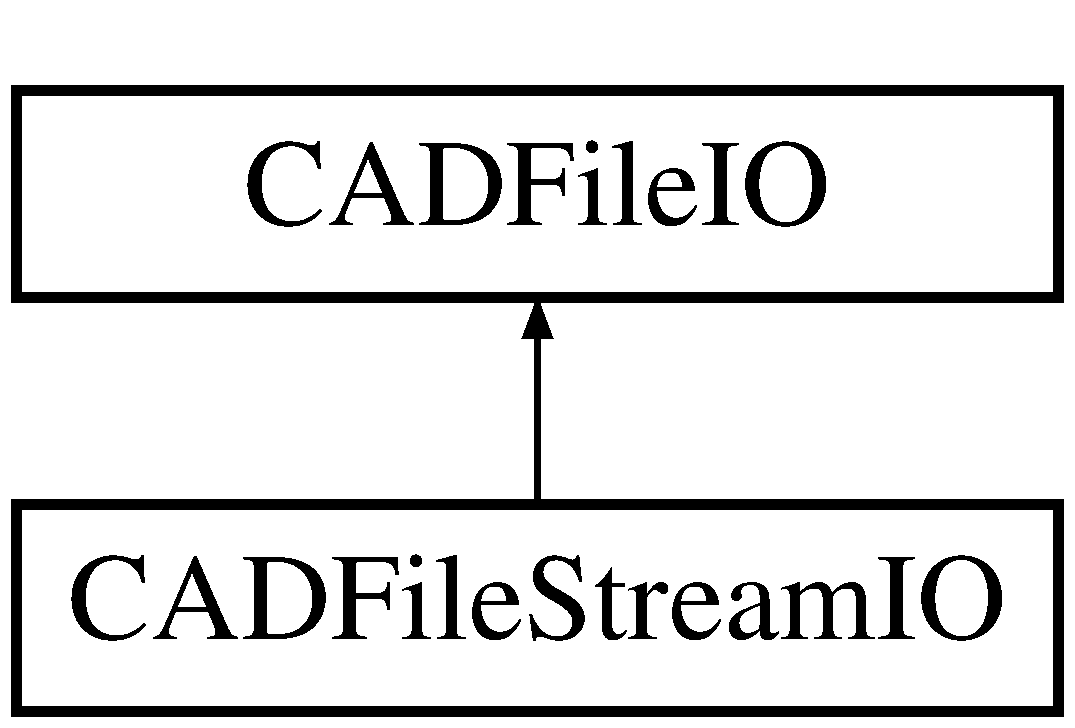
\includegraphics[height=2.000000cm]{class_c_a_d_file_stream_i_o}
\end{center}
\end{figure}
\subsection*{Public Member Functions}
\begin{DoxyCompactItemize}
\item 
{\bfseries C\+A\+D\+File\+Stream\+IO} (const char $\ast$psz\+File\+Path)\hypertarget{class_c_a_d_file_stream_i_o_aac4069683e72c7d74edf95bafa829a02}{}\label{class_c_a_d_file_stream_i_o_aac4069683e72c7d74edf95bafa829a02}

\item 
virtual const char $\ast$ {\bfseries Read\+Line} () override\hypertarget{class_c_a_d_file_stream_i_o_a8cf14e8b59f3b51964b7cc9d0bf10fc2}{}\label{class_c_a_d_file_stream_i_o_a8cf14e8b59f3b51964b7cc9d0bf10fc2}

\item 
virtual bool {\bfseries Eof} () override\hypertarget{class_c_a_d_file_stream_i_o_aa8ec0880bf9a6d2e86f6863926d90906}{}\label{class_c_a_d_file_stream_i_o_aa8ec0880bf9a6d2e86f6863926d90906}

\item 
virtual bool {\bfseries Open} (int mode) override\hypertarget{class_c_a_d_file_stream_i_o_aa7a02c8adebcb02b098b53967ea04ea4}{}\label{class_c_a_d_file_stream_i_o_aa7a02c8adebcb02b098b53967ea04ea4}

\item 
virtual bool {\bfseries Close} () override\hypertarget{class_c_a_d_file_stream_i_o_acc82311b6d85e44d998f941cd075febf}{}\label{class_c_a_d_file_stream_i_o_acc82311b6d85e44d998f941cd075febf}

\item 
virtual int {\bfseries Seek} (long int offset, \hyperlink{class_c_a_d_file_i_o_ac02f709414ed2d228f8dfdabb4eb1b4f}{Seek\+Origin} origin) override\hypertarget{class_c_a_d_file_stream_i_o_a6b7f640fc6ee987ecc76c37dce2e8668}{}\label{class_c_a_d_file_stream_i_o_a6b7f640fc6ee987ecc76c37dce2e8668}

\item 
virtual long int {\bfseries Tell} () override\hypertarget{class_c_a_d_file_stream_i_o_ab7c16d1785e12909a1c5374f007a69db}{}\label{class_c_a_d_file_stream_i_o_ab7c16d1785e12909a1c5374f007a69db}

\item 
virtual size\+\_\+t {\bfseries Read} (void $\ast$ptr, size\+\_\+t size) override\hypertarget{class_c_a_d_file_stream_i_o_a7c294d9ecca566774a4edf2b6d154ade}{}\label{class_c_a_d_file_stream_i_o_a7c294d9ecca566774a4edf2b6d154ade}

\item 
virtual size\+\_\+t {\bfseries Write} (void $\ast$ptr, size\+\_\+t size) override\hypertarget{class_c_a_d_file_stream_i_o_a6898435bc03c202769bd73d3db362c66}{}\label{class_c_a_d_file_stream_i_o_a6898435bc03c202769bd73d3db362c66}

\item 
virtual void {\bfseries Rewind} () override\hypertarget{class_c_a_d_file_stream_i_o_aaee39d2f0a12625895f31f2f548f7b93}{}\label{class_c_a_d_file_stream_i_o_aaee39d2f0a12625895f31f2f548f7b93}

\end{DoxyCompactItemize}
\subsection*{Protected Attributes}
\begin{DoxyCompactItemize}
\item 
std\+::ifstream {\bfseries m\+\_\+o\+File\+Stream}\hypertarget{class_c_a_d_file_stream_i_o_ad7a150910d7f2d1502d85263ceff709f}{}\label{class_c_a_d_file_stream_i_o_ad7a150910d7f2d1502d85263ceff709f}

\end{DoxyCompactItemize}
\subsection*{Additional Inherited Members}


The documentation for this class was generated from the following files\+:\begin{DoxyCompactItemize}
\item 
cadfilestreamio.\+h\item 
cadfilestreamio.\+cpp\end{DoxyCompactItemize}

\hypertarget{class_c_a_d_geometry}{}\section{C\+A\+D\+Geometry Class Reference}
\label{class_c_a_d_geometry}\index{C\+A\+D\+Geometry@{C\+A\+D\+Geometry}}


Base C\+AD geometry class.  




{\ttfamily \#include $<$cadgeometry.\+h$>$}

Inheritance diagram for C\+A\+D\+Geometry\+:\begin{figure}[H]
\begin{center}
\leavevmode
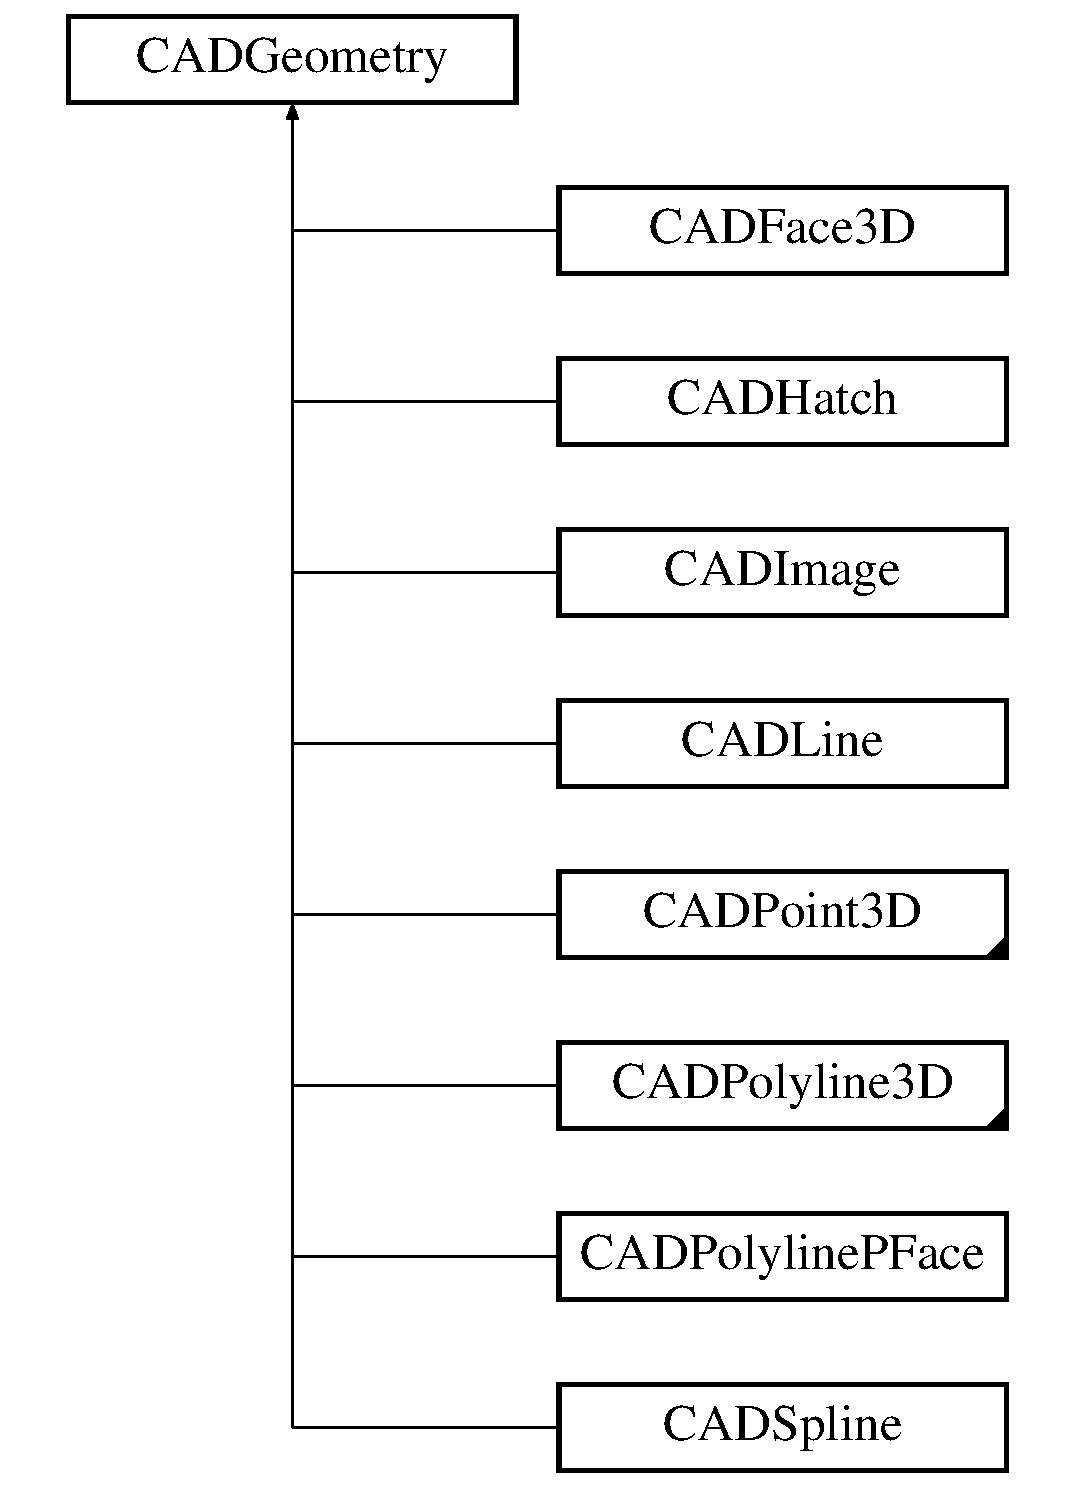
\includegraphics[height=9.000000cm]{class_c_a_d_geometry}
\end{center}
\end{figure}
\subsection*{Public Types}
\begin{DoxyCompactItemize}
\item 
enum \hyperlink{class_c_a_d_geometry_a0515ed61d3514d528f78b8ba6c4fc5f3}{Geometry\+Type} \{ \\*
{\bfseries U\+N\+D\+E\+F\+I\+N\+ED} = 0, 
{\bfseries P\+O\+I\+NT}, 
{\bfseries C\+I\+R\+C\+LE}, 
{\bfseries L\+W\+P\+O\+L\+Y\+L\+I\+NE}, 
\\*
{\bfseries E\+L\+L\+I\+P\+SE}, 
{\bfseries L\+I\+NE}, 
{\bfseries P\+O\+L\+Y\+L\+I\+N\+E3D}, 
{\bfseries T\+E\+XT}, 
\\*
{\bfseries A\+RC}, 
{\bfseries S\+P\+L\+I\+NE}, 
{\bfseries S\+O\+L\+ID}, 
{\bfseries R\+AY}, 
\\*
{\bfseries H\+A\+T\+CH}, 
{\bfseries I\+M\+A\+GE}, 
{\bfseries M\+T\+E\+XT}, 
{\bfseries M\+L\+I\+NE}, 
\\*
{\bfseries X\+L\+I\+NE}, 
{\bfseries F\+A\+C\+E3D}, 
{\bfseries P\+O\+L\+Y\+L\+I\+N\+E\+\_\+\+P\+F\+A\+CE}
 \}\hypertarget{class_c_a_d_geometry_a0515ed61d3514d528f78b8ba6c4fc5f3}{}\label{class_c_a_d_geometry_a0515ed61d3514d528f78b8ba6c4fc5f3}
\begin{DoxyCompactList}\small\item\em The C\+AD geometry types enum. \end{DoxyCompactList}
\end{DoxyCompactItemize}
\subsection*{Public Member Functions}
\begin{DoxyCompactItemize}
\item 
enum \hyperlink{class_c_a_d_geometry_a0515ed61d3514d528f78b8ba6c4fc5f3}{Geometry\+Type} {\bfseries get\+Type} () const \hypertarget{class_c_a_d_geometry_a17ef31adb00b91060cf27595c8df6330}{}\label{class_c_a_d_geometry_a17ef31adb00b91060cf27595c8df6330}

\item 
double {\bfseries get\+Thickness} () const \hypertarget{class_c_a_d_geometry_afb804aa9994b188d8ea4728076c29964}{}\label{class_c_a_d_geometry_afb804aa9994b188d8ea4728076c29964}

\item 
void {\bfseries set\+Thickness} (double thicknes)\hypertarget{class_c_a_d_geometry_abd3022d752e37dac79b92519a15a7fe2}{}\label{class_c_a_d_geometry_abd3022d752e37dac79b92519a15a7fe2}

\item 
\hyperlink{struct_r_g_b_color}{R\+G\+B\+Color} {\bfseries get\+Color} () const \hypertarget{class_c_a_d_geometry_a1f77b5cdf9479129ccbc69d19be5d65e}{}\label{class_c_a_d_geometry_a1f77b5cdf9479129ccbc69d19be5d65e}

\item 
void {\bfseries set\+Color} (int A\+C\+I\+Color\+Index)\hypertarget{class_c_a_d_geometry_a894393c4f6fece4b7e9256aaa5448770}{}\label{class_c_a_d_geometry_a894393c4f6fece4b7e9256aaa5448770}

\item 
virtual void {\bfseries print} () const  =0\hypertarget{class_c_a_d_geometry_aece81ef419d3ad207171bcca57a097dd}{}\label{class_c_a_d_geometry_aece81ef419d3ad207171bcca57a097dd}

\end{DoxyCompactItemize}
\subsection*{Protected Attributes}
\begin{DoxyCompactItemize}
\item 
enum \hyperlink{class_c_a_d_geometry_a0515ed61d3514d528f78b8ba6c4fc5f3}{Geometry\+Type} {\bfseries geometry\+Type}\hypertarget{class_c_a_d_geometry_a34a284842b50d41052f7abc396ed7f91}{}\label{class_c_a_d_geometry_a34a284842b50d41052f7abc396ed7f91}

\item 
double {\bfseries thickness}\hypertarget{class_c_a_d_geometry_acbd206b728d8f720c3d0ac76ccdd0d33}{}\label{class_c_a_d_geometry_acbd206b728d8f720c3d0ac76ccdd0d33}

\item 
\hyperlink{struct_r_g_b_color}{R\+G\+B\+Color} {\bfseries geometry\+\_\+color}\hypertarget{class_c_a_d_geometry_a0d8a3754c859cc103c7ca839d14f279c}{}\label{class_c_a_d_geometry_a0d8a3754c859cc103c7ca839d14f279c}

\end{DoxyCompactItemize}


\subsection{Detailed Description}
Base C\+AD geometry class. 

The documentation for this class was generated from the following files\+:\begin{DoxyCompactItemize}
\item 
cadgeometry.\+h\item 
cadgeometry.\+cpp\end{DoxyCompactItemize}

\hypertarget{class_c_a_d_handle}{}\section{C\+A\+D\+Handle Class Reference}
\label{class_c_a_d_handle}\index{C\+A\+D\+Handle@{C\+A\+D\+Handle}}
\subsection*{Public Member Functions}
\begin{DoxyCompactItemize}
\item 
{\bfseries C\+A\+D\+Handle} (unsigned char code\+In=0)\hypertarget{class_c_a_d_handle_a2424aa7d4d11c24b3226f96d80fbb401}{}\label{class_c_a_d_handle_a2424aa7d4d11c24b3226f96d80fbb401}

\item 
{\bfseries C\+A\+D\+Handle} (const \hyperlink{class_c_a_d_handle}{C\+A\+D\+Handle} \&other)\hypertarget{class_c_a_d_handle_a60fb09aa441674c631b51d09cb858e01}{}\label{class_c_a_d_handle_a60fb09aa441674c631b51d09cb858e01}

\item 
\hyperlink{class_c_a_d_handle}{C\+A\+D\+Handle} \& {\bfseries operator=} (const \hyperlink{class_c_a_d_handle}{C\+A\+D\+Handle} \&other)\hypertarget{class_c_a_d_handle_ab70cf076a65b1f3d29e1d2410422dd12}{}\label{class_c_a_d_handle_ab70cf076a65b1f3d29e1d2410422dd12}

\item 
void {\bfseries add\+Offset} (unsigned char val)\hypertarget{class_c_a_d_handle_af5e7a2a57b6fd75da2cf5dae3a6e6e62}{}\label{class_c_a_d_handle_af5e7a2a57b6fd75da2cf5dae3a6e6e62}

\item 
bool {\bfseries is\+Null} () const \hypertarget{class_c_a_d_handle_aef7cb1ebb89c9542326f031078a05cf2}{}\label{class_c_a_d_handle_aef7cb1ebb89c9542326f031078a05cf2}

\item 
long {\bfseries get\+As\+Long} () const \hypertarget{class_c_a_d_handle_ad520f166b8f666deab857ea3a53d4c58}{}\label{class_c_a_d_handle_ad520f166b8f666deab857ea3a53d4c58}

\item 
long {\bfseries get\+As\+Long} (const \hyperlink{class_c_a_d_handle}{C\+A\+D\+Handle} \&ref\+\_\+handle) const \hypertarget{class_c_a_d_handle_a953b7872ab5082b8c76a04ad53836bc5}{}\label{class_c_a_d_handle_a953b7872ab5082b8c76a04ad53836bc5}

\end{DoxyCompactItemize}
\subsection*{Protected Attributes}
\begin{DoxyCompactItemize}
\item 
unsigned char {\bfseries code}\hypertarget{class_c_a_d_handle_ad787161f5d4f182e36439177f5324bcd}{}\label{class_c_a_d_handle_ad787161f5d4f182e36439177f5324bcd}

\item 
std\+::vector$<$ unsigned char $>$ {\bfseries handle\+Or\+Offset}\hypertarget{class_c_a_d_handle_a285ef4bd94fa410b53744b764545162b}{}\label{class_c_a_d_handle_a285ef4bd94fa410b53744b764545162b}

\end{DoxyCompactItemize}


The documentation for this class was generated from the following files\+:\begin{DoxyCompactItemize}
\item 
cadheader.\+h\item 
cadheader.\+cpp\end{DoxyCompactItemize}

\hypertarget{class_c_a_d_hatch}{}\section{C\+A\+D\+Hatch Class Reference}
\label{class_c_a_d_hatch}\index{C\+A\+D\+Hatch@{C\+A\+D\+Hatch}}


Geometry class which represents Hatch.  




{\ttfamily \#include $<$cadgeometry.\+h$>$}

Inheritance diagram for C\+A\+D\+Hatch\+:\begin{figure}[H]
\begin{center}
\leavevmode
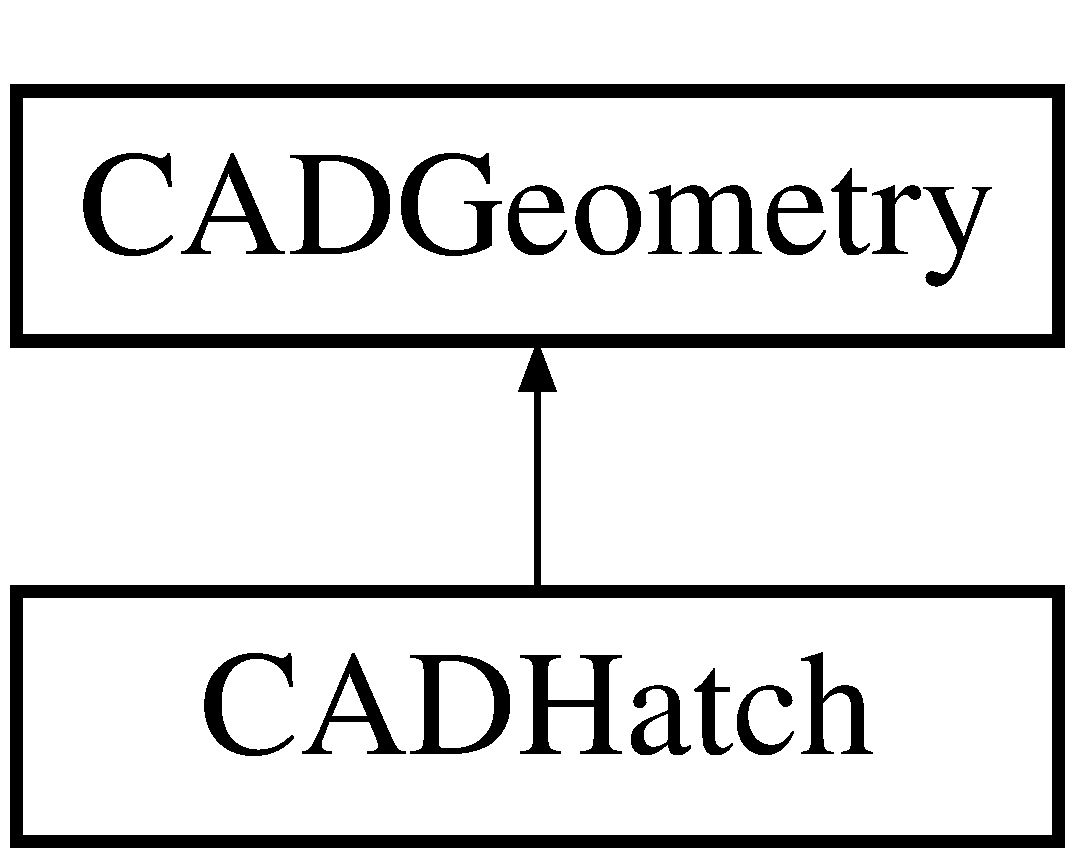
\includegraphics[height=2.000000cm]{class_c_a_d_hatch}
\end{center}
\end{figure}
\subsection*{Additional Inherited Members}


\subsection{Detailed Description}
Geometry class which represents Hatch. 

The documentation for this class was generated from the following files\+:\begin{DoxyCompactItemize}
\item 
cadgeometry.\+h\item 
cadgeometry.\+cpp\end{DoxyCompactItemize}

\hypertarget{class_c_a_d_header}{}\section{C\+A\+D\+Header Class Reference}
\label{class_c_a_d_header}\index{C\+A\+D\+Header@{C\+A\+D\+Header}}


The common C\+AD header class.  




{\ttfamily \#include $<$cadheader.\+h$>$}

\subsection*{Public Types}
\begin{DoxyCompactItemize}
\item 
enum \hyperlink{class_c_a_d_header_abd894aab7aa85b4c4634e67fb93d6886}{C\+A\+D\+Header\+Constants} \{ \\*
\hyperlink{class_c_a_d_header_abd894aab7aa85b4c4634e67fb93d6886ac570bb6faa7e12a10313aded00349764}{O\+P\+E\+N\+C\+A\+D\+V\+ER} = 1, 
\hyperlink{class_c_a_d_header_abd894aab7aa85b4c4634e67fb93d6886a08eac45804230354d6b972f5a9981971}{A\+C\+A\+D\+M\+A\+I\+N\+T\+V\+ER}, 
\hyperlink{class_c_a_d_header_abd894aab7aa85b4c4634e67fb93d6886a7cb3808df0a44802acb276850d312f1b}{A\+C\+A\+D\+V\+ER}, 
\hyperlink{class_c_a_d_header_abd894aab7aa85b4c4634e67fb93d6886a914b5e6703ac3ae3ba2ad1d8bcc6175e}{A\+N\+G\+B\+A\+SE}, 
\\*
\hyperlink{class_c_a_d_header_abd894aab7aa85b4c4634e67fb93d6886abcc055b7295d45575da28eae50f7f302}{A\+N\+G\+D\+IR}, 
\hyperlink{class_c_a_d_header_abd894aab7aa85b4c4634e67fb93d6886ae8aa631aff58cf84d03bd77da4c50473}{A\+T\+T\+M\+O\+DE}, 
\hyperlink{class_c_a_d_header_abd894aab7aa85b4c4634e67fb93d6886a8cc860ea44c317a03d4dd81a57017c58}{A\+T\+T\+R\+EQ}, 
\hyperlink{class_c_a_d_header_abd894aab7aa85b4c4634e67fb93d6886aeaa7a19dab0af3cb33e7c151bdaced04}{A\+T\+T\+D\+IA}, 
\\*
\hyperlink{class_c_a_d_header_abd894aab7aa85b4c4634e67fb93d6886affaf0b90f87d06c32805139104125920}{A\+U\+N\+I\+TS}, 
\hyperlink{class_c_a_d_header_abd894aab7aa85b4c4634e67fb93d6886a41913505a805581218882d8117d6c63b}{A\+U\+P\+R\+EC}, 
\hyperlink{class_c_a_d_header_abd894aab7aa85b4c4634e67fb93d6886ace72893b71d488480334f9f49434a784}{C\+E\+C\+O\+L\+OR}, 
\hyperlink{class_c_a_d_header_abd894aab7aa85b4c4634e67fb93d6886a54b0492ee3fd90097137c82f5971f674}{C\+E\+L\+T\+S\+C\+A\+LE}, 
\\*
\hyperlink{class_c_a_d_header_abd894aab7aa85b4c4634e67fb93d6886a4239205cf0507d30e15d16a437ff95e5}{C\+E\+L\+T\+Y\+PE}, 
\hyperlink{class_c_a_d_header_abd894aab7aa85b4c4634e67fb93d6886a6e76da81b5369a9b9fd5a2e7c1771a06}{C\+E\+L\+W\+E\+I\+G\+HT}, 
\hyperlink{class_c_a_d_header_abd894aab7aa85b4c4634e67fb93d6886a465dae989fc175e2946fd056631ecb12}{C\+E\+P\+S\+N\+ID}, 
\hyperlink{class_c_a_d_header_abd894aab7aa85b4c4634e67fb93d6886ab7f7c6192148fc397662116c93e240ef}{C\+E\+P\+S\+N\+T\+Y\+PE}, 
\\*
\hyperlink{class_c_a_d_header_abd894aab7aa85b4c4634e67fb93d6886aa76898ce968f9195b2bad9cd15e53135}{C\+H\+A\+M\+F\+E\+RA}, 
\hyperlink{class_c_a_d_header_abd894aab7aa85b4c4634e67fb93d6886a92be5ad05fd62029256d6e9189cd0423}{C\+H\+A\+M\+F\+E\+RB}, 
\hyperlink{class_c_a_d_header_abd894aab7aa85b4c4634e67fb93d6886abd950cc26f3278de1f188122d98d7e91}{C\+H\+A\+M\+F\+E\+RC}, 
\hyperlink{class_c_a_d_header_abd894aab7aa85b4c4634e67fb93d6886a6df5e6b1b201bcafb618b54a0b466464}{C\+H\+A\+M\+F\+E\+RD}, 
\\*
\hyperlink{class_c_a_d_header_abd894aab7aa85b4c4634e67fb93d6886a8671da84e5d297bba5ed682cb3a35bfd}{C\+L\+A\+Y\+ER}, 
\hyperlink{class_c_a_d_header_abd894aab7aa85b4c4634e67fb93d6886af56740ddb035e586bfc4e0dd2eb69c07}{C\+M\+L\+J\+U\+ST}, 
\hyperlink{class_c_a_d_header_abd894aab7aa85b4c4634e67fb93d6886aa434f94f9538ff6d49b1f332280f157f}{C\+M\+L\+S\+C\+A\+LE}, 
\hyperlink{class_c_a_d_header_abd894aab7aa85b4c4634e67fb93d6886a43580a83274342d1c9f5db3387991920}{C\+M\+L\+S\+T\+Y\+LE}, 
\\*
\hyperlink{class_c_a_d_header_abd894aab7aa85b4c4634e67fb93d6886a38e1d0a624c0bec121ba548e04af675f}{C\+S\+H\+A\+D\+OW}, 
\hyperlink{class_c_a_d_header_abd894aab7aa85b4c4634e67fb93d6886a1af09f968b84b10fbae183e9dda8e7d9}{D\+I\+M\+A\+D\+EC}, 
\hyperlink{class_c_a_d_header_abd894aab7aa85b4c4634e67fb93d6886a7b1884767d6d6d497d13e07a217e5956}{D\+I\+M\+A\+LT}, 
\hyperlink{class_c_a_d_header_abd894aab7aa85b4c4634e67fb93d6886a69e81b4a4932f714034bba1ab6a44e81}{D\+I\+M\+A\+L\+TD}, 
\\*
\hyperlink{class_c_a_d_header_abd894aab7aa85b4c4634e67fb93d6886aa3ea717e4f3efb9b31c2e133e235b790}{D\+I\+M\+A\+L\+TF}, 
\hyperlink{class_c_a_d_header_abd894aab7aa85b4c4634e67fb93d6886a7f3fc9dbba0b8d985c9ac415e0d34e9a}{D\+I\+M\+A\+L\+T\+R\+ND}, 
\hyperlink{class_c_a_d_header_abd894aab7aa85b4c4634e67fb93d6886a57f8b6dadd0218acd4a4d1137a7dae9a}{D\+I\+M\+A\+L\+T\+TD}, 
\hyperlink{class_c_a_d_header_abd894aab7aa85b4c4634e67fb93d6886a8a3517d84a3b6ef6e0c3fc16746f4eae}{D\+I\+M\+A\+L\+T\+TZ}, 
\\*
\hyperlink{class_c_a_d_header_abd894aab7aa85b4c4634e67fb93d6886a676bbba20b2092ea6d0abc231dc31b2d}{D\+I\+M\+A\+L\+TU}, 
\hyperlink{class_c_a_d_header_abd894aab7aa85b4c4634e67fb93d6886a3ce7061f52ab9718cc62c0078ce9d24e}{D\+I\+M\+A\+L\+TZ}, 
\hyperlink{class_c_a_d_header_abd894aab7aa85b4c4634e67fb93d6886ab3af0953d44cd4241efc386e788aa3d7}{D\+I\+M\+A\+P\+O\+ST}, 
\hyperlink{class_c_a_d_header_abd894aab7aa85b4c4634e67fb93d6886ab617c127464445b85c569c2045f16fcd}{D\+I\+M\+A\+SO}, 
\\*
\hyperlink{class_c_a_d_header_abd894aab7aa85b4c4634e67fb93d6886a94a37e359554c9f3a888b2c5de3cc580}{D\+I\+M\+A\+S\+S\+OC}, 
\hyperlink{class_c_a_d_header_abd894aab7aa85b4c4634e67fb93d6886aec207abcb0e4d1e9d6c538a87b7c0b73}{D\+I\+M\+A\+SZ}, 
\hyperlink{class_c_a_d_header_abd894aab7aa85b4c4634e67fb93d6886ad765da78e92fe997cca7c1b2c592f580}{D\+I\+M\+A\+T\+F\+IT}, 
\hyperlink{class_c_a_d_header_abd894aab7aa85b4c4634e67fb93d6886ab13da86ce0e3438558ee113c5dbfe4fe}{D\+I\+M\+A\+U\+N\+IT}, 
\\*
\hyperlink{class_c_a_d_header_abd894aab7aa85b4c4634e67fb93d6886a866553a56a8f144a0b3fbdf43c753c85}{D\+I\+M\+A\+Z\+IN}, 
\hyperlink{class_c_a_d_header_abd894aab7aa85b4c4634e67fb93d6886abc5664d77a2e45666c09e9862b546920}{D\+I\+M\+B\+LK}, 
\hyperlink{class_c_a_d_header_abd894aab7aa85b4c4634e67fb93d6886a9f465d9407bcec2a976f25e9a36339ad}{D\+I\+M\+B\+L\+K1}, 
\hyperlink{class_c_a_d_header_abd894aab7aa85b4c4634e67fb93d6886adb8d8963f36798f902f276e8091c1050}{D\+I\+M\+B\+L\+K2}, 
\\*
\hyperlink{class_c_a_d_header_abd894aab7aa85b4c4634e67fb93d6886ac73edd9add46d1a954ceaca50c5d18a1}{D\+I\+M\+C\+EN}, 
\hyperlink{class_c_a_d_header_abd894aab7aa85b4c4634e67fb93d6886a9efebc2669e92af02a55df46d7c1bda0}{D\+I\+M\+C\+L\+RD}, 
\hyperlink{class_c_a_d_header_abd894aab7aa85b4c4634e67fb93d6886ace78d776397db84da7fa1176efcd73b2}{D\+I\+M\+C\+L\+RE}, 
\hyperlink{class_c_a_d_header_abd894aab7aa85b4c4634e67fb93d6886ada33abc8dd3608e2b5aabcf7763b7a14}{D\+I\+M\+C\+L\+RT}, 
\\*
\hyperlink{class_c_a_d_header_abd894aab7aa85b4c4634e67fb93d6886a687ebc12b1a661d8c1b2ed7cee2299f2}{D\+I\+M\+D\+EC}, 
\hyperlink{class_c_a_d_header_abd894aab7aa85b4c4634e67fb93d6886a1482ed5b5dfd18bba76479d856c01950}{D\+I\+M\+D\+LE}, 
\hyperlink{class_c_a_d_header_abd894aab7aa85b4c4634e67fb93d6886af139a1b63dd2d93784aef97ae9b4d55e}{D\+I\+M\+D\+LI}, 
\hyperlink{class_c_a_d_header_abd894aab7aa85b4c4634e67fb93d6886a0473ac1a18e859c0ae58c24a085c7aca}{D\+I\+M\+D\+S\+EP}, 
\\*
\hyperlink{class_c_a_d_header_abd894aab7aa85b4c4634e67fb93d6886a9598b8806c1cff8eb280a27048b95c12}{D\+I\+M\+E\+XE}, 
\hyperlink{class_c_a_d_header_abd894aab7aa85b4c4634e67fb93d6886af4f602686e381d9e61da1f3d7177caad}{D\+I\+M\+E\+XO}, 
\hyperlink{class_c_a_d_header_abd894aab7aa85b4c4634e67fb93d6886a7a449b422e0e2fa92df674a6d8e84ecd}{D\+I\+M\+F\+AC}, 
\hyperlink{class_c_a_d_header_abd894aab7aa85b4c4634e67fb93d6886ac03300484d341ee71b9c648b600f08e4}{D\+I\+M\+G\+AP}, 
\\*
\hyperlink{class_c_a_d_header_abd894aab7aa85b4c4634e67fb93d6886a4e3839a44dee79ecf03939b3900e454c}{D\+I\+M\+J\+U\+ST}, 
\hyperlink{class_c_a_d_header_abd894aab7aa85b4c4634e67fb93d6886abb1299cb3fb61a8c34eaec06be4cc095}{D\+I\+M\+L\+D\+R\+B\+LK}, 
\hyperlink{class_c_a_d_header_abd894aab7aa85b4c4634e67fb93d6886af9f9761c672a41e4e736212fd5942a4a}{D\+I\+M\+L\+F\+AC}, 
\hyperlink{class_c_a_d_header_abd894aab7aa85b4c4634e67fb93d6886a1476f0e0fb38b9c70dce9eb0c674d58d}{D\+I\+M\+L\+IM}, 
\\*
\hyperlink{class_c_a_d_header_abd894aab7aa85b4c4634e67fb93d6886a8d8347db70dc7f66335dc27c83feda3b}{D\+I\+M\+L\+U\+N\+IT}, 
\hyperlink{class_c_a_d_header_abd894aab7aa85b4c4634e67fb93d6886aeacf8893f9ce9bf285aa555ee7494d04}{D\+I\+M\+L\+WD}, 
\hyperlink{class_c_a_d_header_abd894aab7aa85b4c4634e67fb93d6886a4ee6a6cd95762d0398172a18fc4cdc5d}{D\+I\+M\+L\+WE}, 
\hyperlink{class_c_a_d_header_abd894aab7aa85b4c4634e67fb93d6886afbd978578868969456b557466588a629}{D\+I\+M\+P\+O\+ST}, 
\\*
\hyperlink{class_c_a_d_header_abd894aab7aa85b4c4634e67fb93d6886a8114511828160b6cb5a531f8e4a8a640}{D\+I\+M\+R\+ND}, 
\hyperlink{class_c_a_d_header_abd894aab7aa85b4c4634e67fb93d6886a0b192097bf5fd49eb8c9d4b4ba7b6a9b}{D\+I\+M\+S\+AH}, 
\hyperlink{class_c_a_d_header_abd894aab7aa85b4c4634e67fb93d6886a020ae1301863dbcddaebd54ec2942074}{D\+I\+M\+S\+C\+A\+LE}, 
\hyperlink{class_c_a_d_header_abd894aab7aa85b4c4634e67fb93d6886ae432f0e77584022f0b2cbf15b385947c}{D\+I\+M\+S\+D1}, 
\\*
\hyperlink{class_c_a_d_header_abd894aab7aa85b4c4634e67fb93d6886ae9969bdac45add0b1e5abffb5b2f191b}{D\+I\+M\+S\+D2}, 
\hyperlink{class_c_a_d_header_abd894aab7aa85b4c4634e67fb93d6886adbd9808d07a12bf767e288901d410fd4}{D\+I\+M\+S\+E1}, 
\hyperlink{class_c_a_d_header_abd894aab7aa85b4c4634e67fb93d6886a2f35827a49b3b4f7b55129f3f9b6bf66}{D\+I\+M\+S\+E2}, 
\hyperlink{class_c_a_d_header_abd894aab7aa85b4c4634e67fb93d6886a3eaf77d9741c3207c6a60d4f58d317fc}{D\+I\+M\+S\+HO}, 
\\*
\hyperlink{class_c_a_d_header_abd894aab7aa85b4c4634e67fb93d6886a2f96ab587a533d69c27c67d4e2c65963}{D\+I\+M\+S\+O\+XD}, 
\hyperlink{class_c_a_d_header_abd894aab7aa85b4c4634e67fb93d6886a7390bf45cba0b6275768e21dc592c920}{D\+I\+M\+S\+T\+Y\+LE}, 
\hyperlink{class_c_a_d_header_abd894aab7aa85b4c4634e67fb93d6886aabe4434794dc20cb9813761c07b25481}{D\+I\+M\+T\+AD}, 
\hyperlink{class_c_a_d_header_abd894aab7aa85b4c4634e67fb93d6886a17978b1cefa950e913e9f7b37492150b}{D\+I\+M\+T\+D\+EC}, 
\\*
\hyperlink{class_c_a_d_header_abd894aab7aa85b4c4634e67fb93d6886a04abec802fc66a450ca0ec0e648c5184}{D\+I\+M\+T\+F\+AC}, 
\hyperlink{class_c_a_d_header_abd894aab7aa85b4c4634e67fb93d6886acecc4886020d2ed1ada226b67ac6e0d1}{D\+I\+M\+T\+IH}, 
\hyperlink{class_c_a_d_header_abd894aab7aa85b4c4634e67fb93d6886a04f66c86c0eb24ab6c2f3f5feb58b5ca}{D\+I\+M\+T\+IX}, 
\hyperlink{class_c_a_d_header_abd894aab7aa85b4c4634e67fb93d6886aacff260f281dbaa5b95c425e12dfb019}{D\+I\+M\+TM}, 
\\*
\hyperlink{class_c_a_d_header_abd894aab7aa85b4c4634e67fb93d6886a3cbb25735b68f093809fb9ea01db7e5d}{D\+I\+M\+T\+M\+O\+VE}, 
\hyperlink{class_c_a_d_header_abd894aab7aa85b4c4634e67fb93d6886a378df39d0ebea264e144ad7819b5d60b}{D\+I\+M\+T\+O\+FL}, 
\hyperlink{class_c_a_d_header_abd894aab7aa85b4c4634e67fb93d6886a067b6df52e133b6fbbb56b5b5200248e}{D\+I\+M\+T\+OH}, 
\hyperlink{class_c_a_d_header_abd894aab7aa85b4c4634e67fb93d6886a382acabaf4b27cb5a880547ccf2511fc}{D\+I\+M\+T\+OL}, 
\\*
\hyperlink{class_c_a_d_header_abd894aab7aa85b4c4634e67fb93d6886a559aafe3cb45cb88e0e4339761956d9c}{D\+I\+M\+T\+O\+LJ}, 
\hyperlink{class_c_a_d_header_abd894aab7aa85b4c4634e67fb93d6886a6f4933ba50455974519a4d0f5fd27fec}{D\+I\+M\+TP}, 
\hyperlink{class_c_a_d_header_abd894aab7aa85b4c4634e67fb93d6886a40035435e79526f44df98ea541209917}{D\+I\+M\+T\+SZ}, 
\hyperlink{class_c_a_d_header_abd894aab7aa85b4c4634e67fb93d6886a060ece3d757784a446731b0e8ebd859a}{D\+I\+M\+T\+VP}, 
\\*
\hyperlink{class_c_a_d_header_abd894aab7aa85b4c4634e67fb93d6886a3223469c7cb866d22d389b45060a920a}{D\+I\+M\+T\+X\+S\+TY}, 
\hyperlink{class_c_a_d_header_abd894aab7aa85b4c4634e67fb93d6886a9f93c170199ee719a94ed7dcb482d8c3}{D\+I\+M\+T\+XT}, 
\hyperlink{class_c_a_d_header_abd894aab7aa85b4c4634e67fb93d6886a68c9a8fdd8634ef564eb40b29a7ce014}{D\+I\+M\+T\+Z\+IN}, 
\hyperlink{class_c_a_d_header_abd894aab7aa85b4c4634e67fb93d6886a296f52bfbcf9bfd3846c2766078d871c}{D\+I\+M\+U\+PT}, 
\\*
\hyperlink{class_c_a_d_header_abd894aab7aa85b4c4634e67fb93d6886a35307893fd6f5cd7af23123a47c2b93e}{D\+I\+M\+Z\+IN}, 
\hyperlink{class_c_a_d_header_abd894aab7aa85b4c4634e67fb93d6886a2531728e27a69698ebdab51abaca2caf}{D\+I\+S\+P\+S\+I\+LH}, 
\hyperlink{class_c_a_d_header_abd894aab7aa85b4c4634e67fb93d6886a3b1911bf3fcdd053b27fe718b71e317d}{D\+R\+A\+G\+VS}, 
\hyperlink{class_c_a_d_header_abd894aab7aa85b4c4634e67fb93d6886a7d8393f3c06479f6db9a789ad6937bcf}{D\+W\+G\+C\+O\+D\+E\+P\+A\+GE}, 
\\*
\hyperlink{class_c_a_d_header_abd894aab7aa85b4c4634e67fb93d6886a30f263bb82409f50d3738441dea6e207}{E\+L\+E\+V\+A\+T\+I\+ON}, 
\hyperlink{class_c_a_d_header_abd894aab7aa85b4c4634e67fb93d6886a7b17b801f1c9f39f7f9f5c67be4fc5fc}{E\+N\+D\+C\+A\+PS}, 
\hyperlink{class_c_a_d_header_abd894aab7aa85b4c4634e67fb93d6886aafa05d1c11168e2ebed258aff81d8d51}{E\+X\+T\+M\+AX}, 
\hyperlink{class_c_a_d_header_abd894aab7aa85b4c4634e67fb93d6886afba4e43bf29f7dcf76c34e3134ced73c}{E\+X\+T\+M\+IN}, 
\\*
\hyperlink{class_c_a_d_header_abd894aab7aa85b4c4634e67fb93d6886a2b22d44ac28f419e1393790986ea292d}{E\+X\+T\+N\+A\+M\+ES}, 
\hyperlink{class_c_a_d_header_abd894aab7aa85b4c4634e67fb93d6886aed813e7f842a510975a70b9011fadd97}{F\+I\+L\+L\+E\+T\+R\+AD}, 
\hyperlink{class_c_a_d_header_abd894aab7aa85b4c4634e67fb93d6886ac8948c5714edbd842719aff4bc179139}{F\+I\+L\+L\+M\+O\+DE}, 
\hyperlink{class_c_a_d_header_abd894aab7aa85b4c4634e67fb93d6886a5b049d1bdddd729d5c50f8b4329d868f}{F\+I\+N\+G\+E\+R\+P\+R\+I\+N\+T\+G\+U\+ID}, 
\\*
\hyperlink{class_c_a_d_header_abd894aab7aa85b4c4634e67fb93d6886a228b8cc6b7683b1089fcb78a6ed54027}{H\+A\+L\+O\+G\+AP}, 
\hyperlink{class_c_a_d_header_abd894aab7aa85b4c4634e67fb93d6886a8350730cc6af4e40d5f221cbef7db728}{H\+A\+N\+D\+S\+E\+ED}, 
\hyperlink{class_c_a_d_header_abd894aab7aa85b4c4634e67fb93d6886a75327037466fbd7ebadc7dd94e3c8cd6}{H\+I\+D\+E\+T\+E\+XT}, 
\hyperlink{class_c_a_d_header_abd894aab7aa85b4c4634e67fb93d6886a9654d04ccd7e6bdceffbe51f9c37849c}{H\+Y\+P\+E\+R\+L\+I\+N\+K\+B\+A\+SE}, 
\\*
\hyperlink{class_c_a_d_header_abd894aab7aa85b4c4634e67fb93d6886a943570b77842628b772b43aded0b1b05}{I\+N\+D\+E\+X\+C\+TL}, 
\hyperlink{class_c_a_d_header_abd894aab7aa85b4c4634e67fb93d6886abac70dd41c3ee084f5c49b9f6b732041}{I\+N\+S\+B\+A\+SE}, 
\hyperlink{class_c_a_d_header_abd894aab7aa85b4c4634e67fb93d6886a5d91e3ef97387612b04d10c8b85595a4}{I\+N\+S\+U\+N\+I\+TS}, 
\hyperlink{class_c_a_d_header_abd894aab7aa85b4c4634e67fb93d6886afd091aea346a0a74d2b8caad565e51c2}{I\+N\+T\+E\+R\+F\+E\+R\+E\+C\+O\+L\+OR}, 
\\*
\hyperlink{class_c_a_d_header_abd894aab7aa85b4c4634e67fb93d6886a462fdeee3a1d9f39f15a29ecebfb8822}{I\+N\+T\+E\+R\+F\+E\+R\+E\+O\+B\+J\+VS}, 
\hyperlink{class_c_a_d_header_abd894aab7aa85b4c4634e67fb93d6886aa64f3fb3349df32b55d546c491392122}{I\+N\+T\+E\+R\+F\+E\+R\+E\+V\+P\+VS}, 
\hyperlink{class_c_a_d_header_abd894aab7aa85b4c4634e67fb93d6886ac73763bf067503d98e4e48b56d46bdaf}{I\+N\+T\+E\+R\+S\+E\+C\+T\+I\+O\+N\+C\+O\+L\+OR}, 
\hyperlink{class_c_a_d_header_abd894aab7aa85b4c4634e67fb93d6886af573c1944f92a7e33f87fc20a428517b}{I\+N\+T\+E\+R\+S\+E\+C\+T\+I\+O\+N\+D\+I\+S\+P\+L\+AY}, 
\\*
\hyperlink{class_c_a_d_header_abd894aab7aa85b4c4634e67fb93d6886ad958e38c5235cb2627bf85763e71143f}{J\+O\+I\+N\+S\+T\+Y\+LE}, 
\hyperlink{class_c_a_d_header_abd894aab7aa85b4c4634e67fb93d6886a55c6aca5cb40ebabe375fd0eab885856}{L\+I\+M\+C\+H\+E\+CK}, 
\hyperlink{class_c_a_d_header_abd894aab7aa85b4c4634e67fb93d6886a125515dabcdb939961f5f8f72997867d}{L\+I\+M\+M\+AX}, 
\hyperlink{class_c_a_d_header_abd894aab7aa85b4c4634e67fb93d6886ac3495533519a545050e84196dde65c3f}{L\+I\+M\+M\+IN}, 
\\*
\hyperlink{class_c_a_d_header_abd894aab7aa85b4c4634e67fb93d6886a74fe9dec505bc43ce0cb4433226f551f}{L\+T\+S\+C\+A\+LE}, 
\hyperlink{class_c_a_d_header_abd894aab7aa85b4c4634e67fb93d6886ad4a8a24e3b3a5bf9ee68431e15b3985c}{L\+U\+N\+I\+TS}, 
\hyperlink{class_c_a_d_header_abd894aab7aa85b4c4634e67fb93d6886aac8eb1d489784b33e4b6cf3772cca2e9}{L\+U\+P\+R\+EC}, 
\hyperlink{class_c_a_d_header_abd894aab7aa85b4c4634e67fb93d6886a9350112285e7d0cefa12c2703c0013a2}{L\+W\+D\+I\+S\+P\+L\+AY}, 
\\*
\hyperlink{class_c_a_d_header_abd894aab7aa85b4c4634e67fb93d6886ab4641c79c45f7caa73ee61387d6ff72f}{M\+A\+X\+A\+C\+T\+VP}, 
\hyperlink{class_c_a_d_header_abd894aab7aa85b4c4634e67fb93d6886ac82af6f66bfdf203381e511e2ccbda3f}{M\+E\+A\+S\+U\+R\+E\+M\+E\+NT}, 
\hyperlink{class_c_a_d_header_abd894aab7aa85b4c4634e67fb93d6886a8e25cca479ee85520ece2a62a93ee775}{M\+E\+NU}, 
\hyperlink{class_c_a_d_header_abd894aab7aa85b4c4634e67fb93d6886ab9c819d5f3d2b0a9182344c2c98b20d1}{M\+I\+R\+R\+T\+E\+XT}, 
\\*
\hyperlink{class_c_a_d_header_abd894aab7aa85b4c4634e67fb93d6886a2d78a3c49c635a923203efc313d1c968}{O\+B\+S\+C\+O\+L\+OR}, 
\hyperlink{class_c_a_d_header_abd894aab7aa85b4c4634e67fb93d6886a716cfa454794e6a9b4b43faa7767b2c1}{O\+B\+S\+L\+T\+Y\+PE}, 
\hyperlink{class_c_a_d_header_abd894aab7aa85b4c4634e67fb93d6886a20a2feb84bc2d160bd16202916b64e6b}{O\+R\+T\+H\+O\+M\+O\+DE}, 
\hyperlink{class_c_a_d_header_abd894aab7aa85b4c4634e67fb93d6886aaf8996048afb6a49c007d0746a4ed309}{P\+D\+M\+O\+DE}, 
\\*
\hyperlink{class_c_a_d_header_abd894aab7aa85b4c4634e67fb93d6886aecc0a6540b6ae33499f4c6f4ef560a6a}{P\+D\+S\+I\+ZE}, 
\hyperlink{class_c_a_d_header_abd894aab7aa85b4c4634e67fb93d6886a350e657af362566eb7a00a66e3ef0f3a}{P\+E\+L\+E\+V\+A\+T\+I\+ON}, 
\hyperlink{class_c_a_d_header_abd894aab7aa85b4c4634e67fb93d6886a55b1c9882cb14afb4d666042ca9392c7}{P\+E\+X\+T\+M\+AX}, 
\hyperlink{class_c_a_d_header_abd894aab7aa85b4c4634e67fb93d6886af382c325f89233336ddf5d7e20d40cd3}{P\+E\+X\+T\+M\+IN}, 
\\*
\hyperlink{class_c_a_d_header_abd894aab7aa85b4c4634e67fb93d6886a6cc3a5f3142799d716854fe53402aef0}{P\+I\+N\+S\+B\+A\+SE}, 
\hyperlink{class_c_a_d_header_abd894aab7aa85b4c4634e67fb93d6886a474630b41af9b90392333e69011bf3ca}{P\+L\+I\+M\+C\+H\+E\+CK}, 
\hyperlink{class_c_a_d_header_abd894aab7aa85b4c4634e67fb93d6886a5aa564a99534fc8d583117f95fba5395}{P\+L\+I\+M\+M\+AX}, 
\hyperlink{class_c_a_d_header_abd894aab7aa85b4c4634e67fb93d6886adea675c00346f03ebf5ce19e83a5b0fa}{P\+L\+I\+M\+M\+IN}, 
\\*
\hyperlink{class_c_a_d_header_abd894aab7aa85b4c4634e67fb93d6886a717cfd50b8c6710d7b63ed252871c0fc}{P\+L\+I\+N\+E\+G\+EN}, 
\hyperlink{class_c_a_d_header_abd894aab7aa85b4c4634e67fb93d6886a6fa1bcddff8cd3b096f64643d7eb2d93}{P\+L\+I\+N\+E\+W\+ID}, 
\hyperlink{class_c_a_d_header_abd894aab7aa85b4c4634e67fb93d6886ac9b6ac3088c11c3e386dd220eff6ed5a}{P\+R\+O\+J\+E\+C\+T\+N\+A\+ME}, 
\hyperlink{class_c_a_d_header_abd894aab7aa85b4c4634e67fb93d6886ae877ef963bc68f5d41f734066cbcd4b4}{P\+R\+O\+X\+Y\+G\+R\+A\+P\+H\+I\+CS}, 
\\*
\hyperlink{class_c_a_d_header_abd894aab7aa85b4c4634e67fb93d6886a5d1d63da87d30431c36bf968f381613c}{P\+S\+L\+T\+S\+C\+A\+LE}, 
\hyperlink{class_c_a_d_header_abd894aab7aa85b4c4634e67fb93d6886a69c6e9ec01d115782c287592e79c525f}{P\+S\+T\+Y\+L\+E\+M\+O\+DE}, 
\hyperlink{class_c_a_d_header_abd894aab7aa85b4c4634e67fb93d6886a71c3465a156fa31e31211dce87be2415}{P\+S\+V\+P\+S\+C\+A\+LE}, 
\hyperlink{class_c_a_d_header_abd894aab7aa85b4c4634e67fb93d6886a106c6316a7f145d03eff37817beb141a}{P\+U\+C\+S\+B\+A\+SE}, 
\\*
\hyperlink{class_c_a_d_header_abd894aab7aa85b4c4634e67fb93d6886ac29607e9495ab59773c0794729dd10cd}{P\+U\+C\+S\+N\+A\+ME}, 
\hyperlink{class_c_a_d_header_abd894aab7aa85b4c4634e67fb93d6886ad758d1fd46a102c49151235aa4d5a85b}{P\+U\+C\+S\+O\+RG}, 
\hyperlink{class_c_a_d_header_abd894aab7aa85b4c4634e67fb93d6886a2d4da9654033cafa52e91313d531f619}{P\+U\+C\+S\+O\+R\+G\+B\+A\+CK}, 
\hyperlink{class_c_a_d_header_abd894aab7aa85b4c4634e67fb93d6886a4f3408a06a9c73de18c3175d94baa094}{P\+U\+C\+S\+O\+R\+G\+B\+O\+T\+T\+OM}, 
\\*
\hyperlink{class_c_a_d_header_abd894aab7aa85b4c4634e67fb93d6886a2409c0f1482d64b39f5095a42b7b3444}{P\+U\+C\+S\+O\+R\+G\+F\+R\+O\+NT}, 
\hyperlink{class_c_a_d_header_abd894aab7aa85b4c4634e67fb93d6886a0f1b1ff39c52461b8e2c1fdc114f26e5}{P\+U\+C\+S\+O\+R\+G\+L\+E\+FT}, 
\hyperlink{class_c_a_d_header_abd894aab7aa85b4c4634e67fb93d6886acd2b4a3057bd04b949fdd4fc9e417b88}{P\+U\+C\+S\+O\+R\+G\+R\+I\+G\+HT}, 
\hyperlink{class_c_a_d_header_abd894aab7aa85b4c4634e67fb93d6886a2f0dbfb41dbe5e9070093d4615d5f00f}{P\+U\+C\+S\+O\+R\+G\+T\+OP}, 
\\*
\hyperlink{class_c_a_d_header_abd894aab7aa85b4c4634e67fb93d6886ae33d7119327ff6bd8d3a68ad18119e50}{P\+U\+C\+S\+O\+R\+T\+H\+O\+R\+EF}, 
\hyperlink{class_c_a_d_header_abd894aab7aa85b4c4634e67fb93d6886a13f84e991a3002c869f4b5f578cbe268}{P\+U\+C\+S\+O\+R\+T\+H\+O\+V\+I\+EW}, 
\hyperlink{class_c_a_d_header_abd894aab7aa85b4c4634e67fb93d6886acd0dc2de2eddca02e3e5ef9ba28df707}{P\+U\+C\+S\+X\+D\+IR}, 
\hyperlink{class_c_a_d_header_abd894aab7aa85b4c4634e67fb93d6886a7a33cb15687b8a798d27adb47991aaf1}{P\+U\+C\+S\+Y\+D\+IR}, 
\\*
\hyperlink{class_c_a_d_header_abd894aab7aa85b4c4634e67fb93d6886a1b42d547886b05e0e4b3f0810b318f6a}{Q\+T\+E\+X\+T\+M\+O\+DE}, 
\hyperlink{class_c_a_d_header_abd894aab7aa85b4c4634e67fb93d6886a29296a568f18a258dc47cd75a6d7cf03}{R\+E\+G\+E\+N\+M\+O\+DE}, 
\hyperlink{class_c_a_d_header_abd894aab7aa85b4c4634e67fb93d6886a7c5f32a4146f387dceb152ca2944038e}{S\+H\+A\+D\+E\+D\+GE}, 
\hyperlink{class_c_a_d_header_abd894aab7aa85b4c4634e67fb93d6886a3f1a8467964e8d829ddc091b478c6c79}{S\+H\+A\+D\+E\+D\+IF}, 
\\*
\hyperlink{class_c_a_d_header_abd894aab7aa85b4c4634e67fb93d6886a9fd9e059bbc8a47725482c2bb8fc3e8e}{S\+H\+A\+D\+O\+W\+P\+L\+A\+N\+E\+L\+O\+C\+A\+T\+I\+ON}, 
\hyperlink{class_c_a_d_header_abd894aab7aa85b4c4634e67fb93d6886ad41348c6e6255f666f63061430e90d05}{S\+K\+E\+T\+C\+H\+I\+NC}, 
\hyperlink{class_c_a_d_header_abd894aab7aa85b4c4634e67fb93d6886aacb2165ff3c4bf51088e2b47bd39ff73}{S\+K\+P\+O\+LY}, 
\hyperlink{class_c_a_d_header_abd894aab7aa85b4c4634e67fb93d6886ab7efa856c989567ef66644e05b3d8334}{S\+O\+R\+T\+E\+N\+TS}, 
\\*
\hyperlink{class_c_a_d_header_abd894aab7aa85b4c4634e67fb93d6886ae6731cea5ff873ba88da93c2971d7003}{S\+P\+L\+I\+N\+E\+S\+E\+GS}, 
\hyperlink{class_c_a_d_header_abd894aab7aa85b4c4634e67fb93d6886a454c87af288f6831ddd3e9ef21aeab9e}{S\+P\+L\+I\+N\+E\+T\+Y\+PE}, 
\hyperlink{class_c_a_d_header_abd894aab7aa85b4c4634e67fb93d6886a220e43663cb21e0e8ca640787b442e03}{S\+U\+R\+F\+T\+A\+B1}, 
\hyperlink{class_c_a_d_header_abd894aab7aa85b4c4634e67fb93d6886a4df698aad8944a5cd8fbae33fe76f248}{S\+U\+R\+F\+T\+A\+B2}, 
\\*
\hyperlink{class_c_a_d_header_abd894aab7aa85b4c4634e67fb93d6886aec2d15b2339c02d5798049ae6c1aeb3f}{S\+U\+R\+F\+T\+Y\+PE}, 
\hyperlink{class_c_a_d_header_abd894aab7aa85b4c4634e67fb93d6886ae3960f8bda99114c123b63c56f0f766a}{S\+U\+R\+FU}, 
\hyperlink{class_c_a_d_header_abd894aab7aa85b4c4634e67fb93d6886a02c02f09bee8e376086fbc806ba1fcfb}{S\+U\+R\+FV}, 
\hyperlink{class_c_a_d_header_abd894aab7aa85b4c4634e67fb93d6886a53985e9ed978cfb35930a710c4351f1f}{T\+D\+C\+R\+E\+A\+TE}, 
\\*
\hyperlink{class_c_a_d_header_abd894aab7aa85b4c4634e67fb93d6886a60852c0f83b55c19076a3768c772c176}{T\+D\+I\+N\+D\+WG}, 
\hyperlink{class_c_a_d_header_abd894aab7aa85b4c4634e67fb93d6886a6b048e7996bf2468ba7a698fb8f34864}{T\+D\+U\+C\+R\+E\+A\+TE}, 
\hyperlink{class_c_a_d_header_abd894aab7aa85b4c4634e67fb93d6886a2901376ecb684fe1c440562f15eb73f3}{T\+D\+U\+P\+D\+A\+TE}, 
\hyperlink{class_c_a_d_header_abd894aab7aa85b4c4634e67fb93d6886a29b7127bbffbdccb9e36665aeb5c98f2}{T\+D\+U\+S\+R\+T\+I\+M\+ER}, 
\\*
\hyperlink{class_c_a_d_header_abd894aab7aa85b4c4634e67fb93d6886a8c229fb121cc19b9a94a1765bbbdd440}{T\+D\+U\+U\+P\+D\+A\+TE}, 
\hyperlink{class_c_a_d_header_abd894aab7aa85b4c4634e67fb93d6886a8635c496af40439759037abb70cf2ea8}{T\+E\+X\+T\+S\+I\+ZE}, 
\hyperlink{class_c_a_d_header_abd894aab7aa85b4c4634e67fb93d6886afea5969dcc97c7b2ee630b05352b7c5c}{T\+E\+X\+T\+S\+T\+Y\+LE}, 
\hyperlink{class_c_a_d_header_abd894aab7aa85b4c4634e67fb93d6886a176c8b6bb45d625bbf8791f3a53693ef}{T\+H\+I\+C\+K\+N\+E\+SS}, 
\\*
\hyperlink{class_c_a_d_header_abd894aab7aa85b4c4634e67fb93d6886a212f97594bd177084a59ca91ac47ad20}{T\+I\+L\+E\+M\+O\+DE}, 
\hyperlink{class_c_a_d_header_abd894aab7aa85b4c4634e67fb93d6886a2ab5c71629e35fb2224cc435c60fee36}{T\+R\+A\+C\+E\+W\+ID}, 
\hyperlink{class_c_a_d_header_abd894aab7aa85b4c4634e67fb93d6886ab45224634b324b6695e92f367840af31}{T\+R\+E\+E\+D\+E\+P\+TH}, 
\hyperlink{class_c_a_d_header_abd894aab7aa85b4c4634e67fb93d6886a03cff61ba6eac15372300b8f17759663}{U\+C\+S\+B\+A\+SE}, 
\\*
\hyperlink{class_c_a_d_header_abd894aab7aa85b4c4634e67fb93d6886a79ed8033f1c56abe61fc14a2321daad2}{U\+C\+S\+N\+A\+ME}, 
\hyperlink{class_c_a_d_header_abd894aab7aa85b4c4634e67fb93d6886adfc4bfaebf9567193d6eb775a1c8d736}{U\+C\+S\+O\+RG}, 
\hyperlink{class_c_a_d_header_abd894aab7aa85b4c4634e67fb93d6886ab55107523caef697786632f890280de5}{U\+C\+S\+O\+R\+G\+B\+A\+CK}, 
\hyperlink{class_c_a_d_header_abd894aab7aa85b4c4634e67fb93d6886a434f2b340421e7c797f49444d9373af0}{U\+C\+S\+O\+R\+G\+B\+O\+T\+T\+OM}, 
\\*
\hyperlink{class_c_a_d_header_abd894aab7aa85b4c4634e67fb93d6886a42972f72fef44bb007a6f8f1a681f8f0}{U\+C\+S\+O\+R\+G\+F\+R\+O\+NT}, 
\hyperlink{class_c_a_d_header_abd894aab7aa85b4c4634e67fb93d6886aa201b0578392812d276d9d23a6f8201d}{U\+C\+S\+O\+R\+G\+L\+E\+FT}, 
\hyperlink{class_c_a_d_header_abd894aab7aa85b4c4634e67fb93d6886af4a1a05f29e8276d1bfe2f259b831919}{U\+C\+S\+O\+R\+G\+R\+I\+G\+HT}, 
\hyperlink{class_c_a_d_header_abd894aab7aa85b4c4634e67fb93d6886a9badade58920b72ec3bcd35c44bc1e66}{U\+C\+S\+O\+R\+G\+T\+OP}, 
\\*
\hyperlink{class_c_a_d_header_abd894aab7aa85b4c4634e67fb93d6886a34b979b2dbe7209cf244a6995e0b0869}{U\+C\+S\+O\+R\+T\+H\+O\+R\+EF}, 
\hyperlink{class_c_a_d_header_abd894aab7aa85b4c4634e67fb93d6886a0284925d4cba45f471d418c3e315a82a}{U\+C\+S\+O\+R\+T\+H\+O\+V\+I\+EW}, 
\hyperlink{class_c_a_d_header_abd894aab7aa85b4c4634e67fb93d6886ac52ea9b5dc1a62e2906d519c9ed3144b}{U\+C\+S\+X\+D\+IR}, 
\hyperlink{class_c_a_d_header_abd894aab7aa85b4c4634e67fb93d6886af09f83c7c9f7892d7736a944a2647c76}{U\+C\+S\+Y\+D\+IR}, 
\\*
\hyperlink{class_c_a_d_header_abd894aab7aa85b4c4634e67fb93d6886a2e68d1e84f1eab249e55ba29fba71084}{U\+N\+I\+T\+M\+O\+DE}, 
\hyperlink{class_c_a_d_header_abd894aab7aa85b4c4634e67fb93d6886a9fca09d5ede6f4b269158cfe471dc542}{U\+S\+E\+R\+I1}, 
{\bfseries U\+S\+E\+R\+I2}, 
{\bfseries U\+S\+E\+R\+I3}, 
\\*
{\bfseries U\+S\+E\+R\+I4}, 
{\bfseries U\+S\+E\+R\+I5}, 
\hyperlink{class_c_a_d_header_abd894aab7aa85b4c4634e67fb93d6886a9afa38205aa6eae4bac9fe2a47396fdb}{U\+S\+E\+R\+R1}, 
{\bfseries U\+S\+E\+R\+R2}, 
\\*
{\bfseries U\+S\+E\+R\+R3}, 
{\bfseries U\+S\+E\+R\+R4}, 
{\bfseries U\+S\+E\+R\+R5}, 
\hyperlink{class_c_a_d_header_abd894aab7aa85b4c4634e67fb93d6886af51978c519b55c723d0317200801a312}{U\+S\+R\+T\+I\+M\+ER}, 
\\*
\hyperlink{class_c_a_d_header_abd894aab7aa85b4c4634e67fb93d6886a8b1ac2e7736ee50f9f8d602055be7d61}{V\+E\+R\+S\+I\+O\+N\+G\+U\+ID}, 
\hyperlink{class_c_a_d_header_abd894aab7aa85b4c4634e67fb93d6886abdcc83230c295f567caf2781a8b59ea1}{V\+I\+S\+R\+E\+T\+A\+IN}, 
\hyperlink{class_c_a_d_header_abd894aab7aa85b4c4634e67fb93d6886ab2930a2e265052312bd759bfc0ec6cf1}{W\+O\+R\+L\+D\+V\+I\+EW}, 
\hyperlink{class_c_a_d_header_abd894aab7aa85b4c4634e67fb93d6886a61c00c87ceffb9a84a4b96275fa5d77c}{X\+C\+L\+I\+P\+F\+R\+A\+ME}, 
\\*
\hyperlink{class_c_a_d_header_abd894aab7aa85b4c4634e67fb93d6886abfdc739888ced20da3813e30d448ae18}{X\+E\+D\+IT}, 
{\bfseries S\+P\+L\+F\+R\+A\+ME}, 
\hyperlink{class_c_a_d_header_abd894aab7aa85b4c4634e67fb93d6886a719e06ab0df2ea7ad482857c2a7b4d38}{W\+O\+R\+D\+L\+V\+I\+EW}, 
\hyperlink{class_c_a_d_header_abd894aab7aa85b4c4634e67fb93d6886af40c66b7649167b773cd25621d09b3b5}{P\+E\+L\+L\+I\+P\+SE}, 
\\*
\hyperlink{class_c_a_d_header_abd894aab7aa85b4c4634e67fb93d6886aff7db36e7a077b4bc550fb110c58e2ca}{I\+S\+O\+L\+I\+N\+ES}, 
\hyperlink{class_c_a_d_header_abd894aab7aa85b4c4634e67fb93d6886acfee17d2e52f9520592ce6102e3c7056}{T\+E\+X\+T\+Q\+L\+TY}, 
\hyperlink{class_c_a_d_header_abd894aab7aa85b4c4634e67fb93d6886a182c402edc4f3686229c9edc4afefb8a}{F\+A\+C\+E\+T\+R\+ES}, 
\hyperlink{class_c_a_d_header_abd894aab7aa85b4c4634e67fb93d6886a793cc413cf55a88d06244d08d6918287}{D\+I\+M\+F\+R\+AC}, 
\\*
\hyperlink{class_c_a_d_header_abd894aab7aa85b4c4634e67fb93d6886af93fc410bb58212ad43956fe69c9686e}{O\+L\+E\+S\+T\+A\+R\+T\+UP}, 
\hyperlink{class_c_a_d_header_abd894aab7aa85b4c4634e67fb93d6886ab01373a926d5a25238000a4613058b3e}{S\+T\+Y\+L\+E\+S\+H\+E\+ET}, 
\hyperlink{class_c_a_d_header_abd894aab7aa85b4c4634e67fb93d6886a2dc8dd9f4980b96c154eb3b94987b1b1}{T\+S\+T\+A\+C\+K\+A\+L\+I\+GN}, 
\hyperlink{class_c_a_d_header_abd894aab7aa85b4c4634e67fb93d6886a23c0fec34caffaf827cc89fbd6dc792c}{T\+S\+T\+A\+C\+K\+S\+I\+ZE}, 
\\*
\hyperlink{class_c_a_d_header_abd894aab7aa85b4c4634e67fb93d6886a1e5db9191e11e71875557403e39a2adb}{M\+A\+X\+\_\+\+H\+E\+A\+D\+E\+R\+\_\+\+C\+O\+N\+S\+T\+A\+NT} = 1000
 \}\begin{DoxyCompactList}\small\item\em The C\+AD нeader сonstants enum get from dxf reference\+: \href{http://help.autodesk.com/view/ACD/2016/ENU/?guid=GUID-A85E8E67-27CD-4C59-BE61-4DC9FADBE74A}{\tt http\+://help.\+autodesk.\+com/view/\+A\+C\+D/2016/\+E\+N\+U/?guid=\+G\+U\+I\+D-\/\+A85\+E8\+E67-\/27\+C\+D-\/4\+C59-\/\+B\+E61-\/4\+D\+C9\+F\+A\+D\+B\+E74A}. \end{DoxyCompactList}
\end{DoxyCompactItemize}
\subsection*{Public Member Functions}
\begin{DoxyCompactItemize}
\item 
int \hyperlink{class_c_a_d_header_a473f456d99e96825bb5207a5c4abeaa4}{add\+Value} (short code, const \hyperlink{class_c_a_d_variant}{C\+A\+D\+Variant} \&val)
\begin{DoxyCompactList}\small\item\em Add new value to the C\+AD file header. \end{DoxyCompactList}\item 
int {\bfseries add\+Value} (short code, const char $\ast$val)\hypertarget{class_c_a_d_header_a038229e6e88cabe0cddede5efa7b0323}{}\label{class_c_a_d_header_a038229e6e88cabe0cddede5efa7b0323}

\item 
int {\bfseries add\+Value} (short code, long val)\hypertarget{class_c_a_d_header_ad640a6fc267d3fd0233ec5f75e786e4f}{}\label{class_c_a_d_header_ad640a6fc267d3fd0233ec5f75e786e4f}

\item 
int {\bfseries add\+Value} (short code, int val)\hypertarget{class_c_a_d_header_aef299b22e5974227674f0fa2e827dfc9}{}\label{class_c_a_d_header_aef299b22e5974227674f0fa2e827dfc9}

\item 
int {\bfseries add\+Value} (short code, short val)\hypertarget{class_c_a_d_header_a3189f204e968e731c20e4ca7a684e154}{}\label{class_c_a_d_header_a3189f204e968e731c20e4ca7a684e154}

\item 
int {\bfseries add\+Value} (short code, double val)\hypertarget{class_c_a_d_header_ac78e2f7126160dde71ab2b8d0abe4c37}{}\label{class_c_a_d_header_ac78e2f7126160dde71ab2b8d0abe4c37}

\item 
int {\bfseries add\+Value} (short code, const std\+::string \&val)\hypertarget{class_c_a_d_header_aa34a737e643a1b727f89ff86fdf4ffa1}{}\label{class_c_a_d_header_aa34a737e643a1b727f89ff86fdf4ffa1}

\item 
int {\bfseries add\+Value} (short code, bool val)\hypertarget{class_c_a_d_header_a9c406b04d9e03ccaa6ed0a22bf1c1151}{}\label{class_c_a_d_header_a9c406b04d9e03ccaa6ed0a22bf1c1151}

\item 
int {\bfseries add\+Value} (short code, double x, double y, double z=0)\hypertarget{class_c_a_d_header_a015793c4620fd3323a9021b1f2c2c618}{}\label{class_c_a_d_header_a015793c4620fd3323a9021b1f2c2c618}

\item 
int {\bfseries add\+Value} (short code, long julianday, long milliseconds)\hypertarget{class_c_a_d_header_a2d652dc82fef10ae68e22eec3881eef6}{}\label{class_c_a_d_header_a2d652dc82fef10ae68e22eec3881eef6}

\item 
int {\bfseries get\+Group\+Code} (short code) const \hypertarget{class_c_a_d_header_a4179a7f07f613d7cdb4616682be1f0e6}{}\label{class_c_a_d_header_a4179a7f07f613d7cdb4616682be1f0e6}

\item 
const \hyperlink{class_c_a_d_variant}{C\+A\+D\+Variant} \& {\bfseries get\+Value} (short code, const \hyperlink{class_c_a_d_variant}{C\+A\+D\+Variant} \&val=\hyperlink{class_c_a_d_variant}{C\+A\+D\+Variant}()) const \hypertarget{class_c_a_d_header_a02948a3df4e9ca9d1433ab8bd23001a6}{}\label{class_c_a_d_header_a02948a3df4e9ca9d1433ab8bd23001a6}

\item 
const char $\ast$ {\bfseries get\+Value\+Name} (short code) const \hypertarget{class_c_a_d_header_a16a7d769a8b50940a84f199cae857a55}{}\label{class_c_a_d_header_a16a7d769a8b50940a84f199cae857a55}

\item 
void {\bfseries print} () const \hypertarget{class_c_a_d_header_a3a4a94f0b0bc51a9bdf358e4385ed5c9}{}\label{class_c_a_d_header_a3a4a94f0b0bc51a9bdf358e4385ed5c9}

\end{DoxyCompactItemize}
\subsection*{Protected Attributes}
\begin{DoxyCompactItemize}
\item 
std\+::map$<$ short, \hyperlink{class_c_a_d_variant}{C\+A\+D\+Variant} $>$ {\bfseries values\+Map}\hypertarget{class_c_a_d_header_a264f6f84f2f54d0bc50ca33139b2e8a5}{}\label{class_c_a_d_header_a264f6f84f2f54d0bc50ca33139b2e8a5}

\end{DoxyCompactItemize}


\subsection{Detailed Description}
The common C\+AD header class. 

\subsection{Member Enumeration Documentation}
\index{C\+A\+D\+Header@{C\+A\+D\+Header}!C\+A\+D\+Header\+Constants@{C\+A\+D\+Header\+Constants}}
\index{C\+A\+D\+Header\+Constants@{C\+A\+D\+Header\+Constants}!C\+A\+D\+Header@{C\+A\+D\+Header}}
\subsubsection[{\texorpdfstring{C\+A\+D\+Header\+Constants}{CADHeaderConstants}}]{\setlength{\rightskip}{0pt plus 5cm}enum {\bf C\+A\+D\+Header\+::\+C\+A\+D\+Header\+Constants}}\hypertarget{class_c_a_d_header_abd894aab7aa85b4c4634e67fb93d6886}{}\label{class_c_a_d_header_abd894aab7aa85b4c4634e67fb93d6886}


The C\+AD нeader сonstants enum get from dxf reference\+: \href{http://help.autodesk.com/view/ACD/2016/ENU/?guid=GUID-A85E8E67-27CD-4C59-BE61-4DC9FADBE74A}{\tt http\+://help.\+autodesk.\+com/view/\+A\+C\+D/2016/\+E\+N\+U/?guid=\+G\+U\+I\+D-\/\+A85\+E8\+E67-\/27\+C\+D-\/4\+C59-\/\+B\+E61-\/4\+D\+C9\+F\+A\+D\+B\+E74A}. 

\begin{Desc}
\item[Enumerator]\par
\begin{description}
\index{O\+P\+E\+N\+C\+A\+D\+V\+ER@{O\+P\+E\+N\+C\+A\+D\+V\+ER}!C\+A\+D\+Header@{C\+A\+D\+Header}}\index{C\+A\+D\+Header@{C\+A\+D\+Header}!O\+P\+E\+N\+C\+A\+D\+V\+ER@{O\+P\+E\+N\+C\+A\+D\+V\+ER}}\item[{\em 
O\+P\+E\+N\+C\+A\+D\+V\+ER\hypertarget{class_c_a_d_header_abd894aab7aa85b4c4634e67fb93d6886ac570bb6faa7e12a10313aded00349764}{}\label{class_c_a_d_header_abd894aab7aa85b4c4634e67fb93d6886ac570bb6faa7e12a10313aded00349764}
}]enum C\+A\+D\+Versions value \index{A\+C\+A\+D\+M\+A\+I\+N\+T\+V\+ER@{A\+C\+A\+D\+M\+A\+I\+N\+T\+V\+ER}!C\+A\+D\+Header@{C\+A\+D\+Header}}\index{C\+A\+D\+Header@{C\+A\+D\+Header}!A\+C\+A\+D\+M\+A\+I\+N\+T\+V\+ER@{A\+C\+A\+D\+M\+A\+I\+N\+T\+V\+ER}}\item[{\em 
A\+C\+A\+D\+M\+A\+I\+N\+T\+V\+ER\hypertarget{class_c_a_d_header_abd894aab7aa85b4c4634e67fb93d6886a08eac45804230354d6b972f5a9981971}{}\label{class_c_a_d_header_abd894aab7aa85b4c4634e67fb93d6886a08eac45804230354d6b972f5a9981971}
}]Maintenance version number (should be ignored) \index{A\+C\+A\+D\+V\+ER@{A\+C\+A\+D\+V\+ER}!C\+A\+D\+Header@{C\+A\+D\+Header}}\index{C\+A\+D\+Header@{C\+A\+D\+Header}!A\+C\+A\+D\+V\+ER@{A\+C\+A\+D\+V\+ER}}\item[{\em 
A\+C\+A\+D\+V\+ER\hypertarget{class_c_a_d_header_abd894aab7aa85b4c4634e67fb93d6886a7cb3808df0a44802acb276850d312f1b}{}\label{class_c_a_d_header_abd894aab7aa85b4c4634e67fb93d6886a7cb3808df0a44802acb276850d312f1b}
}]The Auto\+C\+AD drawing database version number\+: A\+C1006 = R10 A\+C1009 = R11 and R12 A\+C1012 = R13 A\+C1014 = R14 A\+C1015 = Auto\+C\+AD 2000 A\+C1018 = Auto\+C\+AD 2004 A\+C1021 = Auto\+C\+AD 2007 A\+C1024 = Auto\+C\+AD 2010 A\+C1027 = Auto\+C\+AD 2013 \index{A\+N\+G\+B\+A\+SE@{A\+N\+G\+B\+A\+SE}!C\+A\+D\+Header@{C\+A\+D\+Header}}\index{C\+A\+D\+Header@{C\+A\+D\+Header}!A\+N\+G\+B\+A\+SE@{A\+N\+G\+B\+A\+SE}}\item[{\em 
A\+N\+G\+B\+A\+SE\hypertarget{class_c_a_d_header_abd894aab7aa85b4c4634e67fb93d6886a914b5e6703ac3ae3ba2ad1d8bcc6175e}{}\label{class_c_a_d_header_abd894aab7aa85b4c4634e67fb93d6886a914b5e6703ac3ae3ba2ad1d8bcc6175e}
}]Angle 0 direction \index{A\+N\+G\+D\+IR@{A\+N\+G\+D\+IR}!C\+A\+D\+Header@{C\+A\+D\+Header}}\index{C\+A\+D\+Header@{C\+A\+D\+Header}!A\+N\+G\+D\+IR@{A\+N\+G\+D\+IR}}\item[{\em 
A\+N\+G\+D\+IR\hypertarget{class_c_a_d_header_abd894aab7aa85b4c4634e67fb93d6886abcc055b7295d45575da28eae50f7f302}{}\label{class_c_a_d_header_abd894aab7aa85b4c4634e67fb93d6886abcc055b7295d45575da28eae50f7f302}
}]1 (Clockwise angles) or 0 (Counterclockwise angles) \index{A\+T\+T\+M\+O\+DE@{A\+T\+T\+M\+O\+DE}!C\+A\+D\+Header@{C\+A\+D\+Header}}\index{C\+A\+D\+Header@{C\+A\+D\+Header}!A\+T\+T\+M\+O\+DE@{A\+T\+T\+M\+O\+DE}}\item[{\em 
A\+T\+T\+M\+O\+DE\hypertarget{class_c_a_d_header_abd894aab7aa85b4c4634e67fb93d6886ae8aa631aff58cf84d03bd77da4c50473}{}\label{class_c_a_d_header_abd894aab7aa85b4c4634e67fb93d6886ae8aa631aff58cf84d03bd77da4c50473}
}]Attribute visibility\+: 0,1,2 \index{A\+T\+T\+R\+EQ@{A\+T\+T\+R\+EQ}!C\+A\+D\+Header@{C\+A\+D\+Header}}\index{C\+A\+D\+Header@{C\+A\+D\+Header}!A\+T\+T\+R\+EQ@{A\+T\+T\+R\+EQ}}\item[{\em 
A\+T\+T\+R\+EQ\hypertarget{class_c_a_d_header_abd894aab7aa85b4c4634e67fb93d6886a8cc860ea44c317a03d4dd81a57017c58}{}\label{class_c_a_d_header_abd894aab7aa85b4c4634e67fb93d6886a8cc860ea44c317a03d4dd81a57017c58}
}]todo\+: \index{A\+T\+T\+D\+IA@{A\+T\+T\+D\+IA}!C\+A\+D\+Header@{C\+A\+D\+Header}}\index{C\+A\+D\+Header@{C\+A\+D\+Header}!A\+T\+T\+D\+IA@{A\+T\+T\+D\+IA}}\item[{\em 
A\+T\+T\+D\+IA\hypertarget{class_c_a_d_header_abd894aab7aa85b4c4634e67fb93d6886aeaa7a19dab0af3cb33e7c151bdaced04}{}\label{class_c_a_d_header_abd894aab7aa85b4c4634e67fb93d6886aeaa7a19dab0af3cb33e7c151bdaced04}
}]todo\+: \index{A\+U\+N\+I\+TS@{A\+U\+N\+I\+TS}!C\+A\+D\+Header@{C\+A\+D\+Header}}\index{C\+A\+D\+Header@{C\+A\+D\+Header}!A\+U\+N\+I\+TS@{A\+U\+N\+I\+TS}}\item[{\em 
A\+U\+N\+I\+TS\hypertarget{class_c_a_d_header_abd894aab7aa85b4c4634e67fb93d6886affaf0b90f87d06c32805139104125920}{}\label{class_c_a_d_header_abd894aab7aa85b4c4634e67fb93d6886affaf0b90f87d06c32805139104125920}
}]Units format for angles \index{A\+U\+P\+R\+EC@{A\+U\+P\+R\+EC}!C\+A\+D\+Header@{C\+A\+D\+Header}}\index{C\+A\+D\+Header@{C\+A\+D\+Header}!A\+U\+P\+R\+EC@{A\+U\+P\+R\+EC}}\item[{\em 
A\+U\+P\+R\+EC\hypertarget{class_c_a_d_header_abd894aab7aa85b4c4634e67fb93d6886a41913505a805581218882d8117d6c63b}{}\label{class_c_a_d_header_abd894aab7aa85b4c4634e67fb93d6886a41913505a805581218882d8117d6c63b}
}]Units precision for angles \index{C\+E\+C\+O\+L\+OR@{C\+E\+C\+O\+L\+OR}!C\+A\+D\+Header@{C\+A\+D\+Header}}\index{C\+A\+D\+Header@{C\+A\+D\+Header}!C\+E\+C\+O\+L\+OR@{C\+E\+C\+O\+L\+OR}}\item[{\em 
C\+E\+C\+O\+L\+OR\hypertarget{class_c_a_d_header_abd894aab7aa85b4c4634e67fb93d6886ace72893b71d488480334f9f49434a784}{}\label{class_c_a_d_header_abd894aab7aa85b4c4634e67fb93d6886ace72893b71d488480334f9f49434a784}
}]0 = B\+Y\+B\+L\+O\+CK; 256 = B\+Y\+L\+A\+Y\+ER \index{C\+E\+L\+T\+S\+C\+A\+LE@{C\+E\+L\+T\+S\+C\+A\+LE}!C\+A\+D\+Header@{C\+A\+D\+Header}}\index{C\+A\+D\+Header@{C\+A\+D\+Header}!C\+E\+L\+T\+S\+C\+A\+LE@{C\+E\+L\+T\+S\+C\+A\+LE}}\item[{\em 
C\+E\+L\+T\+S\+C\+A\+LE\hypertarget{class_c_a_d_header_abd894aab7aa85b4c4634e67fb93d6886a54b0492ee3fd90097137c82f5971f674}{}\label{class_c_a_d_header_abd894aab7aa85b4c4634e67fb93d6886a54b0492ee3fd90097137c82f5971f674}
}]Current entity linetype scale \index{C\+E\+L\+T\+Y\+PE@{C\+E\+L\+T\+Y\+PE}!C\+A\+D\+Header@{C\+A\+D\+Header}}\index{C\+A\+D\+Header@{C\+A\+D\+Header}!C\+E\+L\+T\+Y\+PE@{C\+E\+L\+T\+Y\+PE}}\item[{\em 
C\+E\+L\+T\+Y\+PE\hypertarget{class_c_a_d_header_abd894aab7aa85b4c4634e67fb93d6886a4239205cf0507d30e15d16a437ff95e5}{}\label{class_c_a_d_header_abd894aab7aa85b4c4634e67fb93d6886a4239205cf0507d30e15d16a437ff95e5}
}]Entity linetype name, or B\+Y\+B\+L\+O\+CK or B\+Y\+L\+A\+Y\+ER \index{C\+E\+L\+W\+E\+I\+G\+HT@{C\+E\+L\+W\+E\+I\+G\+HT}!C\+A\+D\+Header@{C\+A\+D\+Header}}\index{C\+A\+D\+Header@{C\+A\+D\+Header}!C\+E\+L\+W\+E\+I\+G\+HT@{C\+E\+L\+W\+E\+I\+G\+HT}}\item[{\em 
C\+E\+L\+W\+E\+I\+G\+HT\hypertarget{class_c_a_d_header_abd894aab7aa85b4c4634e67fb93d6886a6e76da81b5369a9b9fd5a2e7c1771a06}{}\label{class_c_a_d_header_abd894aab7aa85b4c4634e67fb93d6886a6e76da81b5369a9b9fd5a2e7c1771a06}
}]Lineweight of new objects \index{C\+E\+P\+S\+N\+ID@{C\+E\+P\+S\+N\+ID}!C\+A\+D\+Header@{C\+A\+D\+Header}}\index{C\+A\+D\+Header@{C\+A\+D\+Header}!C\+E\+P\+S\+N\+ID@{C\+E\+P\+S\+N\+ID}}\item[{\em 
C\+E\+P\+S\+N\+ID\hypertarget{class_c_a_d_header_abd894aab7aa85b4c4634e67fb93d6886a465dae989fc175e2946fd056631ecb12}{}\label{class_c_a_d_header_abd894aab7aa85b4c4634e67fb93d6886a465dae989fc175e2946fd056631ecb12}
}]Plotstyle handle of new objects; if C\+E\+P\+S\+N\+T\+Y\+PE is 3, then this value indicates the handle \index{C\+E\+P\+S\+N\+T\+Y\+PE@{C\+E\+P\+S\+N\+T\+Y\+PE}!C\+A\+D\+Header@{C\+A\+D\+Header}}\index{C\+A\+D\+Header@{C\+A\+D\+Header}!C\+E\+P\+S\+N\+T\+Y\+PE@{C\+E\+P\+S\+N\+T\+Y\+PE}}\item[{\em 
C\+E\+P\+S\+N\+T\+Y\+PE\hypertarget{class_c_a_d_header_abd894aab7aa85b4c4634e67fb93d6886ab7f7c6192148fc397662116c93e240ef}{}\label{class_c_a_d_header_abd894aab7aa85b4c4634e67fb93d6886ab7f7c6192148fc397662116c93e240ef}
}]Plot style type of new objects\+: 0 = Plot style by layer, 1 = Plot style by block, 2 = Plot style by dictionary default, 3 = Plot style by object I\+D/handle \index{C\+H\+A\+M\+F\+E\+RA@{C\+H\+A\+M\+F\+E\+RA}!C\+A\+D\+Header@{C\+A\+D\+Header}}\index{C\+A\+D\+Header@{C\+A\+D\+Header}!C\+H\+A\+M\+F\+E\+RA@{C\+H\+A\+M\+F\+E\+RA}}\item[{\em 
C\+H\+A\+M\+F\+E\+RA\hypertarget{class_c_a_d_header_abd894aab7aa85b4c4634e67fb93d6886aa76898ce968f9195b2bad9cd15e53135}{}\label{class_c_a_d_header_abd894aab7aa85b4c4634e67fb93d6886aa76898ce968f9195b2bad9cd15e53135}
}]First chamfer distance \index{C\+H\+A\+M\+F\+E\+RB@{C\+H\+A\+M\+F\+E\+RB}!C\+A\+D\+Header@{C\+A\+D\+Header}}\index{C\+A\+D\+Header@{C\+A\+D\+Header}!C\+H\+A\+M\+F\+E\+RB@{C\+H\+A\+M\+F\+E\+RB}}\item[{\em 
C\+H\+A\+M\+F\+E\+RB\hypertarget{class_c_a_d_header_abd894aab7aa85b4c4634e67fb93d6886a92be5ad05fd62029256d6e9189cd0423}{}\label{class_c_a_d_header_abd894aab7aa85b4c4634e67fb93d6886a92be5ad05fd62029256d6e9189cd0423}
}]Second chamfer distance \index{C\+H\+A\+M\+F\+E\+RC@{C\+H\+A\+M\+F\+E\+RC}!C\+A\+D\+Header@{C\+A\+D\+Header}}\index{C\+A\+D\+Header@{C\+A\+D\+Header}!C\+H\+A\+M\+F\+E\+RC@{C\+H\+A\+M\+F\+E\+RC}}\item[{\em 
C\+H\+A\+M\+F\+E\+RC\hypertarget{class_c_a_d_header_abd894aab7aa85b4c4634e67fb93d6886abd950cc26f3278de1f188122d98d7e91}{}\label{class_c_a_d_header_abd894aab7aa85b4c4634e67fb93d6886abd950cc26f3278de1f188122d98d7e91}
}]Chamfer length \index{C\+H\+A\+M\+F\+E\+RD@{C\+H\+A\+M\+F\+E\+RD}!C\+A\+D\+Header@{C\+A\+D\+Header}}\index{C\+A\+D\+Header@{C\+A\+D\+Header}!C\+H\+A\+M\+F\+E\+RD@{C\+H\+A\+M\+F\+E\+RD}}\item[{\em 
C\+H\+A\+M\+F\+E\+RD\hypertarget{class_c_a_d_header_abd894aab7aa85b4c4634e67fb93d6886a6df5e6b1b201bcafb618b54a0b466464}{}\label{class_c_a_d_header_abd894aab7aa85b4c4634e67fb93d6886a6df5e6b1b201bcafb618b54a0b466464}
}]Chamfer angle \index{C\+L\+A\+Y\+ER@{C\+L\+A\+Y\+ER}!C\+A\+D\+Header@{C\+A\+D\+Header}}\index{C\+A\+D\+Header@{C\+A\+D\+Header}!C\+L\+A\+Y\+ER@{C\+L\+A\+Y\+ER}}\item[{\em 
C\+L\+A\+Y\+ER\hypertarget{class_c_a_d_header_abd894aab7aa85b4c4634e67fb93d6886a8671da84e5d297bba5ed682cb3a35bfd}{}\label{class_c_a_d_header_abd894aab7aa85b4c4634e67fb93d6886a8671da84e5d297bba5ed682cb3a35bfd}
}]Current layer name \index{C\+M\+L\+J\+U\+ST@{C\+M\+L\+J\+U\+ST}!C\+A\+D\+Header@{C\+A\+D\+Header}}\index{C\+A\+D\+Header@{C\+A\+D\+Header}!C\+M\+L\+J\+U\+ST@{C\+M\+L\+J\+U\+ST}}\item[{\em 
C\+M\+L\+J\+U\+ST\hypertarget{class_c_a_d_header_abd894aab7aa85b4c4634e67fb93d6886af56740ddb035e586bfc4e0dd2eb69c07}{}\label{class_c_a_d_header_abd894aab7aa85b4c4634e67fb93d6886af56740ddb035e586bfc4e0dd2eb69c07}
}]Current multiline justification\+: 0 = Top; 1 = Middle; 2 = Bottom \index{C\+M\+L\+S\+C\+A\+LE@{C\+M\+L\+S\+C\+A\+LE}!C\+A\+D\+Header@{C\+A\+D\+Header}}\index{C\+A\+D\+Header@{C\+A\+D\+Header}!C\+M\+L\+S\+C\+A\+LE@{C\+M\+L\+S\+C\+A\+LE}}\item[{\em 
C\+M\+L\+S\+C\+A\+LE\hypertarget{class_c_a_d_header_abd894aab7aa85b4c4634e67fb93d6886aa434f94f9538ff6d49b1f332280f157f}{}\label{class_c_a_d_header_abd894aab7aa85b4c4634e67fb93d6886aa434f94f9538ff6d49b1f332280f157f}
}]Current multiline scale \index{C\+M\+L\+S\+T\+Y\+LE@{C\+M\+L\+S\+T\+Y\+LE}!C\+A\+D\+Header@{C\+A\+D\+Header}}\index{C\+A\+D\+Header@{C\+A\+D\+Header}!C\+M\+L\+S\+T\+Y\+LE@{C\+M\+L\+S\+T\+Y\+LE}}\item[{\em 
C\+M\+L\+S\+T\+Y\+LE\hypertarget{class_c_a_d_header_abd894aab7aa85b4c4634e67fb93d6886a43580a83274342d1c9f5db3387991920}{}\label{class_c_a_d_header_abd894aab7aa85b4c4634e67fb93d6886a43580a83274342d1c9f5db3387991920}
}]Current multiline style name \index{C\+S\+H\+A\+D\+OW@{C\+S\+H\+A\+D\+OW}!C\+A\+D\+Header@{C\+A\+D\+Header}}\index{C\+A\+D\+Header@{C\+A\+D\+Header}!C\+S\+H\+A\+D\+OW@{C\+S\+H\+A\+D\+OW}}\item[{\em 
C\+S\+H\+A\+D\+OW\hypertarget{class_c_a_d_header_abd894aab7aa85b4c4634e67fb93d6886a38e1d0a624c0bec121ba548e04af675f}{}\label{class_c_a_d_header_abd894aab7aa85b4c4634e67fb93d6886a38e1d0a624c0bec121ba548e04af675f}
}]Shadow mode for a 3D object\+: 0 = Casts and receives shadows 1 = Casts shadows 2 = Receives shadows 3 = Ignores shadows \index{D\+I\+M\+A\+D\+EC@{D\+I\+M\+A\+D\+EC}!C\+A\+D\+Header@{C\+A\+D\+Header}}\index{C\+A\+D\+Header@{C\+A\+D\+Header}!D\+I\+M\+A\+D\+EC@{D\+I\+M\+A\+D\+EC}}\item[{\em 
D\+I\+M\+A\+D\+EC\hypertarget{class_c_a_d_header_abd894aab7aa85b4c4634e67fb93d6886a1af09f968b84b10fbae183e9dda8e7d9}{}\label{class_c_a_d_header_abd894aab7aa85b4c4634e67fb93d6886a1af09f968b84b10fbae183e9dda8e7d9}
}]Number of precision places displayed in angular dimensions \index{D\+I\+M\+A\+LT@{D\+I\+M\+A\+LT}!C\+A\+D\+Header@{C\+A\+D\+Header}}\index{C\+A\+D\+Header@{C\+A\+D\+Header}!D\+I\+M\+A\+LT@{D\+I\+M\+A\+LT}}\item[{\em 
D\+I\+M\+A\+LT\hypertarget{class_c_a_d_header_abd894aab7aa85b4c4634e67fb93d6886a7b1884767d6d6d497d13e07a217e5956}{}\label{class_c_a_d_header_abd894aab7aa85b4c4634e67fb93d6886a7b1884767d6d6d497d13e07a217e5956}
}]Alternate unit dimensioning performed if nonzero \index{D\+I\+M\+A\+L\+TD@{D\+I\+M\+A\+L\+TD}!C\+A\+D\+Header@{C\+A\+D\+Header}}\index{C\+A\+D\+Header@{C\+A\+D\+Header}!D\+I\+M\+A\+L\+TD@{D\+I\+M\+A\+L\+TD}}\item[{\em 
D\+I\+M\+A\+L\+TD\hypertarget{class_c_a_d_header_abd894aab7aa85b4c4634e67fb93d6886a69e81b4a4932f714034bba1ab6a44e81}{}\label{class_c_a_d_header_abd894aab7aa85b4c4634e67fb93d6886a69e81b4a4932f714034bba1ab6a44e81}
}]Alternate unit decimal places \index{D\+I\+M\+A\+L\+TF@{D\+I\+M\+A\+L\+TF}!C\+A\+D\+Header@{C\+A\+D\+Header}}\index{C\+A\+D\+Header@{C\+A\+D\+Header}!D\+I\+M\+A\+L\+TF@{D\+I\+M\+A\+L\+TF}}\item[{\em 
D\+I\+M\+A\+L\+TF\hypertarget{class_c_a_d_header_abd894aab7aa85b4c4634e67fb93d6886aa3ea717e4f3efb9b31c2e133e235b790}{}\label{class_c_a_d_header_abd894aab7aa85b4c4634e67fb93d6886aa3ea717e4f3efb9b31c2e133e235b790}
}]Alternate unit scale factor \index{D\+I\+M\+A\+L\+T\+R\+ND@{D\+I\+M\+A\+L\+T\+R\+ND}!C\+A\+D\+Header@{C\+A\+D\+Header}}\index{C\+A\+D\+Header@{C\+A\+D\+Header}!D\+I\+M\+A\+L\+T\+R\+ND@{D\+I\+M\+A\+L\+T\+R\+ND}}\item[{\em 
D\+I\+M\+A\+L\+T\+R\+ND\hypertarget{class_c_a_d_header_abd894aab7aa85b4c4634e67fb93d6886a7f3fc9dbba0b8d985c9ac415e0d34e9a}{}\label{class_c_a_d_header_abd894aab7aa85b4c4634e67fb93d6886a7f3fc9dbba0b8d985c9ac415e0d34e9a}
}]Determines rounding of alternate units \index{D\+I\+M\+A\+L\+T\+TD@{D\+I\+M\+A\+L\+T\+TD}!C\+A\+D\+Header@{C\+A\+D\+Header}}\index{C\+A\+D\+Header@{C\+A\+D\+Header}!D\+I\+M\+A\+L\+T\+TD@{D\+I\+M\+A\+L\+T\+TD}}\item[{\em 
D\+I\+M\+A\+L\+T\+TD\hypertarget{class_c_a_d_header_abd894aab7aa85b4c4634e67fb93d6886a57f8b6dadd0218acd4a4d1137a7dae9a}{}\label{class_c_a_d_header_abd894aab7aa85b4c4634e67fb93d6886a57f8b6dadd0218acd4a4d1137a7dae9a}
}]Number of decimal places for tolerance values of an alternate units dimension \index{D\+I\+M\+A\+L\+T\+TZ@{D\+I\+M\+A\+L\+T\+TZ}!C\+A\+D\+Header@{C\+A\+D\+Header}}\index{C\+A\+D\+Header@{C\+A\+D\+Header}!D\+I\+M\+A\+L\+T\+TZ@{D\+I\+M\+A\+L\+T\+TZ}}\item[{\em 
D\+I\+M\+A\+L\+T\+TZ\hypertarget{class_c_a_d_header_abd894aab7aa85b4c4634e67fb93d6886a8a3517d84a3b6ef6e0c3fc16746f4eae}{}\label{class_c_a_d_header_abd894aab7aa85b4c4634e67fb93d6886a8a3517d84a3b6ef6e0c3fc16746f4eae}
}]Controls suppression of zeros for alternate tolerance values\+: 0 = Suppresses zero feet and precisely zero inches 1 = Includes zero feet and precisely zero inches 2 = Includes zero feet and suppresses zero inches 3 = Includes zero inches and suppresses zero feet \index{D\+I\+M\+A\+L\+TU@{D\+I\+M\+A\+L\+TU}!C\+A\+D\+Header@{C\+A\+D\+Header}}\index{C\+A\+D\+Header@{C\+A\+D\+Header}!D\+I\+M\+A\+L\+TU@{D\+I\+M\+A\+L\+TU}}\item[{\em 
D\+I\+M\+A\+L\+TU\hypertarget{class_c_a_d_header_abd894aab7aa85b4c4634e67fb93d6886a676bbba20b2092ea6d0abc231dc31b2d}{}\label{class_c_a_d_header_abd894aab7aa85b4c4634e67fb93d6886a676bbba20b2092ea6d0abc231dc31b2d}
}]Units format for alternate units of all dimension style family members except angular\+: 1 = Scientific 2 = Decimal 3 = Engineering 4 = Architectural (stacked) 5 = Fractional (stacked) 6 = Architectural 7 = Fractional \index{D\+I\+M\+A\+L\+TZ@{D\+I\+M\+A\+L\+TZ}!C\+A\+D\+Header@{C\+A\+D\+Header}}\index{C\+A\+D\+Header@{C\+A\+D\+Header}!D\+I\+M\+A\+L\+TZ@{D\+I\+M\+A\+L\+TZ}}\item[{\em 
D\+I\+M\+A\+L\+TZ\hypertarget{class_c_a_d_header_abd894aab7aa85b4c4634e67fb93d6886a3ce7061f52ab9718cc62c0078ce9d24e}{}\label{class_c_a_d_header_abd894aab7aa85b4c4634e67fb93d6886a3ce7061f52ab9718cc62c0078ce9d24e}
}]Controls suppression of zeros for alternate unit dimension, values\+: 0 = Suppresses zero feet and precisely zero inches 1 = Includes zero feet and precisely zero inches 2 = Includes zero feet and suppresses zero inches 3 = Includes zero inches and suppresses zero feet \index{D\+I\+M\+A\+P\+O\+ST@{D\+I\+M\+A\+P\+O\+ST}!C\+A\+D\+Header@{C\+A\+D\+Header}}\index{C\+A\+D\+Header@{C\+A\+D\+Header}!D\+I\+M\+A\+P\+O\+ST@{D\+I\+M\+A\+P\+O\+ST}}\item[{\em 
D\+I\+M\+A\+P\+O\+ST\hypertarget{class_c_a_d_header_abd894aab7aa85b4c4634e67fb93d6886ab3af0953d44cd4241efc386e788aa3d7}{}\label{class_c_a_d_header_abd894aab7aa85b4c4634e67fb93d6886ab3af0953d44cd4241efc386e788aa3d7}
}]Alternate dimensioning suffix \index{D\+I\+M\+A\+SO@{D\+I\+M\+A\+SO}!C\+A\+D\+Header@{C\+A\+D\+Header}}\index{C\+A\+D\+Header@{C\+A\+D\+Header}!D\+I\+M\+A\+SO@{D\+I\+M\+A\+SO}}\item[{\em 
D\+I\+M\+A\+SO\hypertarget{class_c_a_d_header_abd894aab7aa85b4c4634e67fb93d6886ab617c127464445b85c569c2045f16fcd}{}\label{class_c_a_d_header_abd894aab7aa85b4c4634e67fb93d6886ab617c127464445b85c569c2045f16fcd}
}]1 = Create associative dimensioning, 0 = Draw individual entities \index{D\+I\+M\+A\+S\+S\+OC@{D\+I\+M\+A\+S\+S\+OC}!C\+A\+D\+Header@{C\+A\+D\+Header}}\index{C\+A\+D\+Header@{C\+A\+D\+Header}!D\+I\+M\+A\+S\+S\+OC@{D\+I\+M\+A\+S\+S\+OC}}\item[{\em 
D\+I\+M\+A\+S\+S\+OC\hypertarget{class_c_a_d_header_abd894aab7aa85b4c4634e67fb93d6886a94a37e359554c9f3a888b2c5de3cc580}{}\label{class_c_a_d_header_abd894aab7aa85b4c4634e67fb93d6886a94a37e359554c9f3a888b2c5de3cc580}
}]Controls the associativity of dimension objects\+: 0 = Creates exploded dimensions; there is no association between elements of the dimension, and the lines, arcs, arrowheads, and text of a dimension are drawn as separate objects 1 = Creates non-\/associative dimension objects; the elements of the dimension are formed into a single object, and if the definition point on the object moves, then the dimension value is updated 2 = Creates associative dimension objects; the elements of the dimension are formed into a single object and one or more definition points of the dimension are coupled with association points on geometric objects \index{D\+I\+M\+A\+SZ@{D\+I\+M\+A\+SZ}!C\+A\+D\+Header@{C\+A\+D\+Header}}\index{C\+A\+D\+Header@{C\+A\+D\+Header}!D\+I\+M\+A\+SZ@{D\+I\+M\+A\+SZ}}\item[{\em 
D\+I\+M\+A\+SZ\hypertarget{class_c_a_d_header_abd894aab7aa85b4c4634e67fb93d6886aec207abcb0e4d1e9d6c538a87b7c0b73}{}\label{class_c_a_d_header_abd894aab7aa85b4c4634e67fb93d6886aec207abcb0e4d1e9d6c538a87b7c0b73}
}]Dimensioning arrow size \index{D\+I\+M\+A\+T\+F\+IT@{D\+I\+M\+A\+T\+F\+IT}!C\+A\+D\+Header@{C\+A\+D\+Header}}\index{C\+A\+D\+Header@{C\+A\+D\+Header}!D\+I\+M\+A\+T\+F\+IT@{D\+I\+M\+A\+T\+F\+IT}}\item[{\em 
D\+I\+M\+A\+T\+F\+IT\hypertarget{class_c_a_d_header_abd894aab7aa85b4c4634e67fb93d6886ad765da78e92fe997cca7c1b2c592f580}{}\label{class_c_a_d_header_abd894aab7aa85b4c4634e67fb93d6886ad765da78e92fe997cca7c1b2c592f580}
}]Controls dimension text and arrow placement when space is not sufficient to place both within the extension lines\+: 0 = Places both text and arrows outside extension lines 1 = Moves arrows first, then text 2 = Moves text first, then arrows 3 = Moves either text or arrows, whichever fits best Auto\+C\+AD adds a leader to moved dimension text when D\+I\+M\+T\+M\+O\+VE is set to 1 \index{D\+I\+M\+A\+U\+N\+IT@{D\+I\+M\+A\+U\+N\+IT}!C\+A\+D\+Header@{C\+A\+D\+Header}}\index{C\+A\+D\+Header@{C\+A\+D\+Header}!D\+I\+M\+A\+U\+N\+IT@{D\+I\+M\+A\+U\+N\+IT}}\item[{\em 
D\+I\+M\+A\+U\+N\+IT\hypertarget{class_c_a_d_header_abd894aab7aa85b4c4634e67fb93d6886ab13da86ce0e3438558ee113c5dbfe4fe}{}\label{class_c_a_d_header_abd894aab7aa85b4c4634e67fb93d6886ab13da86ce0e3438558ee113c5dbfe4fe}
}]Angle format for angular dimensions\+: 0 = Decimal degrees 1 = Degrees/minutes/seconds 2 = Gradians 3 = Radians 4 = Surveyor\textquotesingle{}s units \index{D\+I\+M\+A\+Z\+IN@{D\+I\+M\+A\+Z\+IN}!C\+A\+D\+Header@{C\+A\+D\+Header}}\index{C\+A\+D\+Header@{C\+A\+D\+Header}!D\+I\+M\+A\+Z\+IN@{D\+I\+M\+A\+Z\+IN}}\item[{\em 
D\+I\+M\+A\+Z\+IN\hypertarget{class_c_a_d_header_abd894aab7aa85b4c4634e67fb93d6886a866553a56a8f144a0b3fbdf43c753c85}{}\label{class_c_a_d_header_abd894aab7aa85b4c4634e67fb93d6886a866553a56a8f144a0b3fbdf43c753c85}
}]Controls suppression of zeros for angular dimensions\+: 0 = Displays all leading and trailing zeros 1 = Suppresses leading zeros in decimal dimensions 2 = Suppresses trailing zeros in decimal dimensions 3 = Suppresses leading and trailing zeros \index{D\+I\+M\+B\+LK@{D\+I\+M\+B\+LK}!C\+A\+D\+Header@{C\+A\+D\+Header}}\index{C\+A\+D\+Header@{C\+A\+D\+Header}!D\+I\+M\+B\+LK@{D\+I\+M\+B\+LK}}\item[{\em 
D\+I\+M\+B\+LK\hypertarget{class_c_a_d_header_abd894aab7aa85b4c4634e67fb93d6886abc5664d77a2e45666c09e9862b546920}{}\label{class_c_a_d_header_abd894aab7aa85b4c4634e67fb93d6886abc5664d77a2e45666c09e9862b546920}
}]Arrow block name \index{D\+I\+M\+B\+L\+K1@{D\+I\+M\+B\+L\+K1}!C\+A\+D\+Header@{C\+A\+D\+Header}}\index{C\+A\+D\+Header@{C\+A\+D\+Header}!D\+I\+M\+B\+L\+K1@{D\+I\+M\+B\+L\+K1}}\item[{\em 
D\+I\+M\+B\+L\+K1\hypertarget{class_c_a_d_header_abd894aab7aa85b4c4634e67fb93d6886a9f465d9407bcec2a976f25e9a36339ad}{}\label{class_c_a_d_header_abd894aab7aa85b4c4634e67fb93d6886a9f465d9407bcec2a976f25e9a36339ad}
}]First arrow block name \index{D\+I\+M\+B\+L\+K2@{D\+I\+M\+B\+L\+K2}!C\+A\+D\+Header@{C\+A\+D\+Header}}\index{C\+A\+D\+Header@{C\+A\+D\+Header}!D\+I\+M\+B\+L\+K2@{D\+I\+M\+B\+L\+K2}}\item[{\em 
D\+I\+M\+B\+L\+K2\hypertarget{class_c_a_d_header_abd894aab7aa85b4c4634e67fb93d6886adb8d8963f36798f902f276e8091c1050}{}\label{class_c_a_d_header_abd894aab7aa85b4c4634e67fb93d6886adb8d8963f36798f902f276e8091c1050}
}]Second arrow block name \index{D\+I\+M\+C\+EN@{D\+I\+M\+C\+EN}!C\+A\+D\+Header@{C\+A\+D\+Header}}\index{C\+A\+D\+Header@{C\+A\+D\+Header}!D\+I\+M\+C\+EN@{D\+I\+M\+C\+EN}}\item[{\em 
D\+I\+M\+C\+EN\hypertarget{class_c_a_d_header_abd894aab7aa85b4c4634e67fb93d6886ac73edd9add46d1a954ceaca50c5d18a1}{}\label{class_c_a_d_header_abd894aab7aa85b4c4634e67fb93d6886ac73edd9add46d1a954ceaca50c5d18a1}
}]Size of center mark/lines \index{D\+I\+M\+C\+L\+RD@{D\+I\+M\+C\+L\+RD}!C\+A\+D\+Header@{C\+A\+D\+Header}}\index{C\+A\+D\+Header@{C\+A\+D\+Header}!D\+I\+M\+C\+L\+RD@{D\+I\+M\+C\+L\+RD}}\item[{\em 
D\+I\+M\+C\+L\+RD\hypertarget{class_c_a_d_header_abd894aab7aa85b4c4634e67fb93d6886a9efebc2669e92af02a55df46d7c1bda0}{}\label{class_c_a_d_header_abd894aab7aa85b4c4634e67fb93d6886a9efebc2669e92af02a55df46d7c1bda0}
}]Dimension line color\+: range is 0 = B\+Y\+B\+L\+O\+CK; 256 = B\+Y\+L\+A\+Y\+ER \index{D\+I\+M\+C\+L\+RE@{D\+I\+M\+C\+L\+RE}!C\+A\+D\+Header@{C\+A\+D\+Header}}\index{C\+A\+D\+Header@{C\+A\+D\+Header}!D\+I\+M\+C\+L\+RE@{D\+I\+M\+C\+L\+RE}}\item[{\em 
D\+I\+M\+C\+L\+RE\hypertarget{class_c_a_d_header_abd894aab7aa85b4c4634e67fb93d6886ace78d776397db84da7fa1176efcd73b2}{}\label{class_c_a_d_header_abd894aab7aa85b4c4634e67fb93d6886ace78d776397db84da7fa1176efcd73b2}
}]Dimension extension line color\+: range is 0 = B\+Y\+B\+L\+O\+CK; 256 = B\+Y\+L\+A\+Y\+ER \index{D\+I\+M\+C\+L\+RT@{D\+I\+M\+C\+L\+RT}!C\+A\+D\+Header@{C\+A\+D\+Header}}\index{C\+A\+D\+Header@{C\+A\+D\+Header}!D\+I\+M\+C\+L\+RT@{D\+I\+M\+C\+L\+RT}}\item[{\em 
D\+I\+M\+C\+L\+RT\hypertarget{class_c_a_d_header_abd894aab7aa85b4c4634e67fb93d6886ada33abc8dd3608e2b5aabcf7763b7a14}{}\label{class_c_a_d_header_abd894aab7aa85b4c4634e67fb93d6886ada33abc8dd3608e2b5aabcf7763b7a14}
}]Dimension text color\+: range is 0 = B\+Y\+B\+L\+O\+CK; 256 = B\+Y\+L\+A\+Y\+ER \index{D\+I\+M\+D\+EC@{D\+I\+M\+D\+EC}!C\+A\+D\+Header@{C\+A\+D\+Header}}\index{C\+A\+D\+Header@{C\+A\+D\+Header}!D\+I\+M\+D\+EC@{D\+I\+M\+D\+EC}}\item[{\em 
D\+I\+M\+D\+EC\hypertarget{class_c_a_d_header_abd894aab7aa85b4c4634e67fb93d6886a687ebc12b1a661d8c1b2ed7cee2299f2}{}\label{class_c_a_d_header_abd894aab7aa85b4c4634e67fb93d6886a687ebc12b1a661d8c1b2ed7cee2299f2}
}]Number of decimal places for the tolerance values of a primary units dimension \index{D\+I\+M\+D\+LE@{D\+I\+M\+D\+LE}!C\+A\+D\+Header@{C\+A\+D\+Header}}\index{C\+A\+D\+Header@{C\+A\+D\+Header}!D\+I\+M\+D\+LE@{D\+I\+M\+D\+LE}}\item[{\em 
D\+I\+M\+D\+LE\hypertarget{class_c_a_d_header_abd894aab7aa85b4c4634e67fb93d6886a1482ed5b5dfd18bba76479d856c01950}{}\label{class_c_a_d_header_abd894aab7aa85b4c4634e67fb93d6886a1482ed5b5dfd18bba76479d856c01950}
}]Dimension line extension \index{D\+I\+M\+D\+LI@{D\+I\+M\+D\+LI}!C\+A\+D\+Header@{C\+A\+D\+Header}}\index{C\+A\+D\+Header@{C\+A\+D\+Header}!D\+I\+M\+D\+LI@{D\+I\+M\+D\+LI}}\item[{\em 
D\+I\+M\+D\+LI\hypertarget{class_c_a_d_header_abd894aab7aa85b4c4634e67fb93d6886af139a1b63dd2d93784aef97ae9b4d55e}{}\label{class_c_a_d_header_abd894aab7aa85b4c4634e67fb93d6886af139a1b63dd2d93784aef97ae9b4d55e}
}]Dimension line increment \index{D\+I\+M\+D\+S\+EP@{D\+I\+M\+D\+S\+EP}!C\+A\+D\+Header@{C\+A\+D\+Header}}\index{C\+A\+D\+Header@{C\+A\+D\+Header}!D\+I\+M\+D\+S\+EP@{D\+I\+M\+D\+S\+EP}}\item[{\em 
D\+I\+M\+D\+S\+EP\hypertarget{class_c_a_d_header_abd894aab7aa85b4c4634e67fb93d6886a0473ac1a18e859c0ae58c24a085c7aca}{}\label{class_c_a_d_header_abd894aab7aa85b4c4634e67fb93d6886a0473ac1a18e859c0ae58c24a085c7aca}
}]Single-\/character decimal separator used when creating dimensions whose unit format is decimal \index{D\+I\+M\+E\+XE@{D\+I\+M\+E\+XE}!C\+A\+D\+Header@{C\+A\+D\+Header}}\index{C\+A\+D\+Header@{C\+A\+D\+Header}!D\+I\+M\+E\+XE@{D\+I\+M\+E\+XE}}\item[{\em 
D\+I\+M\+E\+XE\hypertarget{class_c_a_d_header_abd894aab7aa85b4c4634e67fb93d6886a9598b8806c1cff8eb280a27048b95c12}{}\label{class_c_a_d_header_abd894aab7aa85b4c4634e67fb93d6886a9598b8806c1cff8eb280a27048b95c12}
}]Extension line extension \index{D\+I\+M\+E\+XO@{D\+I\+M\+E\+XO}!C\+A\+D\+Header@{C\+A\+D\+Header}}\index{C\+A\+D\+Header@{C\+A\+D\+Header}!D\+I\+M\+E\+XO@{D\+I\+M\+E\+XO}}\item[{\em 
D\+I\+M\+E\+XO\hypertarget{class_c_a_d_header_abd894aab7aa85b4c4634e67fb93d6886af4f602686e381d9e61da1f3d7177caad}{}\label{class_c_a_d_header_abd894aab7aa85b4c4634e67fb93d6886af4f602686e381d9e61da1f3d7177caad}
}]Extension line offset \index{D\+I\+M\+F\+AC@{D\+I\+M\+F\+AC}!C\+A\+D\+Header@{C\+A\+D\+Header}}\index{C\+A\+D\+Header@{C\+A\+D\+Header}!D\+I\+M\+F\+AC@{D\+I\+M\+F\+AC}}\item[{\em 
D\+I\+M\+F\+AC\hypertarget{class_c_a_d_header_abd894aab7aa85b4c4634e67fb93d6886a7a449b422e0e2fa92df674a6d8e84ecd}{}\label{class_c_a_d_header_abd894aab7aa85b4c4634e67fb93d6886a7a449b422e0e2fa92df674a6d8e84ecd}
}]Scale factor used to calculate the height of text for dimension fractions and tolerances. Auto\+C\+AD multiplies D\+I\+M\+T\+XT by D\+I\+M\+T\+F\+AC to set the fractional or tolerance text height \index{D\+I\+M\+G\+AP@{D\+I\+M\+G\+AP}!C\+A\+D\+Header@{C\+A\+D\+Header}}\index{C\+A\+D\+Header@{C\+A\+D\+Header}!D\+I\+M\+G\+AP@{D\+I\+M\+G\+AP}}\item[{\em 
D\+I\+M\+G\+AP\hypertarget{class_c_a_d_header_abd894aab7aa85b4c4634e67fb93d6886ac03300484d341ee71b9c648b600f08e4}{}\label{class_c_a_d_header_abd894aab7aa85b4c4634e67fb93d6886ac03300484d341ee71b9c648b600f08e4}
}]Dimension line gap \index{D\+I\+M\+J\+U\+ST@{D\+I\+M\+J\+U\+ST}!C\+A\+D\+Header@{C\+A\+D\+Header}}\index{C\+A\+D\+Header@{C\+A\+D\+Header}!D\+I\+M\+J\+U\+ST@{D\+I\+M\+J\+U\+ST}}\item[{\em 
D\+I\+M\+J\+U\+ST\hypertarget{class_c_a_d_header_abd894aab7aa85b4c4634e67fb93d6886a4e3839a44dee79ecf03939b3900e454c}{}\label{class_c_a_d_header_abd894aab7aa85b4c4634e67fb93d6886a4e3839a44dee79ecf03939b3900e454c}
}]Horizontal dimension text position\+: 0 = Above dimension line and center-\/justified between extension lines 1 = Above dimension line and next to first extension line 2 = Above dimension line and next to second extension line 3 = Above and center-\/justified to first extension line 4 = Above and center-\/justified to second extension line \index{D\+I\+M\+L\+D\+R\+B\+LK@{D\+I\+M\+L\+D\+R\+B\+LK}!C\+A\+D\+Header@{C\+A\+D\+Header}}\index{C\+A\+D\+Header@{C\+A\+D\+Header}!D\+I\+M\+L\+D\+R\+B\+LK@{D\+I\+M\+L\+D\+R\+B\+LK}}\item[{\em 
D\+I\+M\+L\+D\+R\+B\+LK\hypertarget{class_c_a_d_header_abd894aab7aa85b4c4634e67fb93d6886abb1299cb3fb61a8c34eaec06be4cc095}{}\label{class_c_a_d_header_abd894aab7aa85b4c4634e67fb93d6886abb1299cb3fb61a8c34eaec06be4cc095}
}]Arrow block name for leaders \index{D\+I\+M\+L\+F\+AC@{D\+I\+M\+L\+F\+AC}!C\+A\+D\+Header@{C\+A\+D\+Header}}\index{C\+A\+D\+Header@{C\+A\+D\+Header}!D\+I\+M\+L\+F\+AC@{D\+I\+M\+L\+F\+AC}}\item[{\em 
D\+I\+M\+L\+F\+AC\hypertarget{class_c_a_d_header_abd894aab7aa85b4c4634e67fb93d6886af9f9761c672a41e4e736212fd5942a4a}{}\label{class_c_a_d_header_abd894aab7aa85b4c4634e67fb93d6886af9f9761c672a41e4e736212fd5942a4a}
}]Linear measurements scale factor \index{D\+I\+M\+L\+IM@{D\+I\+M\+L\+IM}!C\+A\+D\+Header@{C\+A\+D\+Header}}\index{C\+A\+D\+Header@{C\+A\+D\+Header}!D\+I\+M\+L\+IM@{D\+I\+M\+L\+IM}}\item[{\em 
D\+I\+M\+L\+IM\hypertarget{class_c_a_d_header_abd894aab7aa85b4c4634e67fb93d6886a1476f0e0fb38b9c70dce9eb0c674d58d}{}\label{class_c_a_d_header_abd894aab7aa85b4c4634e67fb93d6886a1476f0e0fb38b9c70dce9eb0c674d58d}
}]Dimension limits generated if nonzero \index{D\+I\+M\+L\+U\+N\+IT@{D\+I\+M\+L\+U\+N\+IT}!C\+A\+D\+Header@{C\+A\+D\+Header}}\index{C\+A\+D\+Header@{C\+A\+D\+Header}!D\+I\+M\+L\+U\+N\+IT@{D\+I\+M\+L\+U\+N\+IT}}\item[{\em 
D\+I\+M\+L\+U\+N\+IT\hypertarget{class_c_a_d_header_abd894aab7aa85b4c4634e67fb93d6886a8d8347db70dc7f66335dc27c83feda3b}{}\label{class_c_a_d_header_abd894aab7aa85b4c4634e67fb93d6886a8d8347db70dc7f66335dc27c83feda3b}
}]Sets units for all dimension types except Angular\+: 1 = Scientific 2 = Decimal 3 = Engineering 4 = Architectural 5 = Fractional 6 = Windows desktop \index{D\+I\+M\+L\+WD@{D\+I\+M\+L\+WD}!C\+A\+D\+Header@{C\+A\+D\+Header}}\index{C\+A\+D\+Header@{C\+A\+D\+Header}!D\+I\+M\+L\+WD@{D\+I\+M\+L\+WD}}\item[{\em 
D\+I\+M\+L\+WD\hypertarget{class_c_a_d_header_abd894aab7aa85b4c4634e67fb93d6886aeacf8893f9ce9bf285aa555ee7494d04}{}\label{class_c_a_d_header_abd894aab7aa85b4c4634e67fb93d6886aeacf8893f9ce9bf285aa555ee7494d04}
}]Dimension line lineweight\+: -\/3 = Standard -\/2 = By\+Layer -\/1 = By\+Block 0-\/211 = an integer representing 100th of mm \index{D\+I\+M\+L\+WE@{D\+I\+M\+L\+WE}!C\+A\+D\+Header@{C\+A\+D\+Header}}\index{C\+A\+D\+Header@{C\+A\+D\+Header}!D\+I\+M\+L\+WE@{D\+I\+M\+L\+WE}}\item[{\em 
D\+I\+M\+L\+WE\hypertarget{class_c_a_d_header_abd894aab7aa85b4c4634e67fb93d6886a4ee6a6cd95762d0398172a18fc4cdc5d}{}\label{class_c_a_d_header_abd894aab7aa85b4c4634e67fb93d6886a4ee6a6cd95762d0398172a18fc4cdc5d}
}]Extension line lineweight\+: -\/3 = Standard -\/2 = By\+Layer -\/1 = By\+Block 0-\/211 = an integer representing 100th of mm \index{D\+I\+M\+P\+O\+ST@{D\+I\+M\+P\+O\+ST}!C\+A\+D\+Header@{C\+A\+D\+Header}}\index{C\+A\+D\+Header@{C\+A\+D\+Header}!D\+I\+M\+P\+O\+ST@{D\+I\+M\+P\+O\+ST}}\item[{\em 
D\+I\+M\+P\+O\+ST\hypertarget{class_c_a_d_header_abd894aab7aa85b4c4634e67fb93d6886afbd978578868969456b557466588a629}{}\label{class_c_a_d_header_abd894aab7aa85b4c4634e67fb93d6886afbd978578868969456b557466588a629}
}]General dimensioning suffix \index{D\+I\+M\+R\+ND@{D\+I\+M\+R\+ND}!C\+A\+D\+Header@{C\+A\+D\+Header}}\index{C\+A\+D\+Header@{C\+A\+D\+Header}!D\+I\+M\+R\+ND@{D\+I\+M\+R\+ND}}\item[{\em 
D\+I\+M\+R\+ND\hypertarget{class_c_a_d_header_abd894aab7aa85b4c4634e67fb93d6886a8114511828160b6cb5a531f8e4a8a640}{}\label{class_c_a_d_header_abd894aab7aa85b4c4634e67fb93d6886a8114511828160b6cb5a531f8e4a8a640}
}]Rounding value for dimension distances \index{D\+I\+M\+S\+AH@{D\+I\+M\+S\+AH}!C\+A\+D\+Header@{C\+A\+D\+Header}}\index{C\+A\+D\+Header@{C\+A\+D\+Header}!D\+I\+M\+S\+AH@{D\+I\+M\+S\+AH}}\item[{\em 
D\+I\+M\+S\+AH\hypertarget{class_c_a_d_header_abd894aab7aa85b4c4634e67fb93d6886a0b192097bf5fd49eb8c9d4b4ba7b6a9b}{}\label{class_c_a_d_header_abd894aab7aa85b4c4634e67fb93d6886a0b192097bf5fd49eb8c9d4b4ba7b6a9b}
}]Use separate arrow blocks if nonzero \index{D\+I\+M\+S\+C\+A\+LE@{D\+I\+M\+S\+C\+A\+LE}!C\+A\+D\+Header@{C\+A\+D\+Header}}\index{C\+A\+D\+Header@{C\+A\+D\+Header}!D\+I\+M\+S\+C\+A\+LE@{D\+I\+M\+S\+C\+A\+LE}}\item[{\em 
D\+I\+M\+S\+C\+A\+LE\hypertarget{class_c_a_d_header_abd894aab7aa85b4c4634e67fb93d6886a020ae1301863dbcddaebd54ec2942074}{}\label{class_c_a_d_header_abd894aab7aa85b4c4634e67fb93d6886a020ae1301863dbcddaebd54ec2942074}
}]Overall dimensioning scale factor \index{D\+I\+M\+S\+D1@{D\+I\+M\+S\+D1}!C\+A\+D\+Header@{C\+A\+D\+Header}}\index{C\+A\+D\+Header@{C\+A\+D\+Header}!D\+I\+M\+S\+D1@{D\+I\+M\+S\+D1}}\item[{\em 
D\+I\+M\+S\+D1\hypertarget{class_c_a_d_header_abd894aab7aa85b4c4634e67fb93d6886ae432f0e77584022f0b2cbf15b385947c}{}\label{class_c_a_d_header_abd894aab7aa85b4c4634e67fb93d6886ae432f0e77584022f0b2cbf15b385947c}
}]Suppression of first extension line\+: 0 = Not suppressed 1 = Suppressed \index{D\+I\+M\+S\+D2@{D\+I\+M\+S\+D2}!C\+A\+D\+Header@{C\+A\+D\+Header}}\index{C\+A\+D\+Header@{C\+A\+D\+Header}!D\+I\+M\+S\+D2@{D\+I\+M\+S\+D2}}\item[{\em 
D\+I\+M\+S\+D2\hypertarget{class_c_a_d_header_abd894aab7aa85b4c4634e67fb93d6886ae9969bdac45add0b1e5abffb5b2f191b}{}\label{class_c_a_d_header_abd894aab7aa85b4c4634e67fb93d6886ae9969bdac45add0b1e5abffb5b2f191b}
}]Suppression of second extension line\+: 0 = Not suppressed 1 = Suppressed \index{D\+I\+M\+S\+E1@{D\+I\+M\+S\+E1}!C\+A\+D\+Header@{C\+A\+D\+Header}}\index{C\+A\+D\+Header@{C\+A\+D\+Header}!D\+I\+M\+S\+E1@{D\+I\+M\+S\+E1}}\item[{\em 
D\+I\+M\+S\+E1\hypertarget{class_c_a_d_header_abd894aab7aa85b4c4634e67fb93d6886adbd9808d07a12bf767e288901d410fd4}{}\label{class_c_a_d_header_abd894aab7aa85b4c4634e67fb93d6886adbd9808d07a12bf767e288901d410fd4}
}]First extension line suppressed if nonzero \index{D\+I\+M\+S\+E2@{D\+I\+M\+S\+E2}!C\+A\+D\+Header@{C\+A\+D\+Header}}\index{C\+A\+D\+Header@{C\+A\+D\+Header}!D\+I\+M\+S\+E2@{D\+I\+M\+S\+E2}}\item[{\em 
D\+I\+M\+S\+E2\hypertarget{class_c_a_d_header_abd894aab7aa85b4c4634e67fb93d6886a2f35827a49b3b4f7b55129f3f9b6bf66}{}\label{class_c_a_d_header_abd894aab7aa85b4c4634e67fb93d6886a2f35827a49b3b4f7b55129f3f9b6bf66}
}]Second extension line suppressed if nonzero \index{D\+I\+M\+S\+HO@{D\+I\+M\+S\+HO}!C\+A\+D\+Header@{C\+A\+D\+Header}}\index{C\+A\+D\+Header@{C\+A\+D\+Header}!D\+I\+M\+S\+HO@{D\+I\+M\+S\+HO}}\item[{\em 
D\+I\+M\+S\+HO\hypertarget{class_c_a_d_header_abd894aab7aa85b4c4634e67fb93d6886a3eaf77d9741c3207c6a60d4f58d317fc}{}\label{class_c_a_d_header_abd894aab7aa85b4c4634e67fb93d6886a3eaf77d9741c3207c6a60d4f58d317fc}
}]1 = Recompute dimensions while dragging 0 = Drag original image \index{D\+I\+M\+S\+O\+XD@{D\+I\+M\+S\+O\+XD}!C\+A\+D\+Header@{C\+A\+D\+Header}}\index{C\+A\+D\+Header@{C\+A\+D\+Header}!D\+I\+M\+S\+O\+XD@{D\+I\+M\+S\+O\+XD}}\item[{\em 
D\+I\+M\+S\+O\+XD\hypertarget{class_c_a_d_header_abd894aab7aa85b4c4634e67fb93d6886a2f96ab587a533d69c27c67d4e2c65963}{}\label{class_c_a_d_header_abd894aab7aa85b4c4634e67fb93d6886a2f96ab587a533d69c27c67d4e2c65963}
}]Suppress outside-\/extensions dimension lines if nonzero \index{D\+I\+M\+S\+T\+Y\+LE@{D\+I\+M\+S\+T\+Y\+LE}!C\+A\+D\+Header@{C\+A\+D\+Header}}\index{C\+A\+D\+Header@{C\+A\+D\+Header}!D\+I\+M\+S\+T\+Y\+LE@{D\+I\+M\+S\+T\+Y\+LE}}\item[{\em 
D\+I\+M\+S\+T\+Y\+LE\hypertarget{class_c_a_d_header_abd894aab7aa85b4c4634e67fb93d6886a7390bf45cba0b6275768e21dc592c920}{}\label{class_c_a_d_header_abd894aab7aa85b4c4634e67fb93d6886a7390bf45cba0b6275768e21dc592c920}
}]Dimension style name \index{D\+I\+M\+T\+AD@{D\+I\+M\+T\+AD}!C\+A\+D\+Header@{C\+A\+D\+Header}}\index{C\+A\+D\+Header@{C\+A\+D\+Header}!D\+I\+M\+T\+AD@{D\+I\+M\+T\+AD}}\item[{\em 
D\+I\+M\+T\+AD\hypertarget{class_c_a_d_header_abd894aab7aa85b4c4634e67fb93d6886aabe4434794dc20cb9813761c07b25481}{}\label{class_c_a_d_header_abd894aab7aa85b4c4634e67fb93d6886aabe4434794dc20cb9813761c07b25481}
}]Text above dimension line if nonzero \index{D\+I\+M\+T\+D\+EC@{D\+I\+M\+T\+D\+EC}!C\+A\+D\+Header@{C\+A\+D\+Header}}\index{C\+A\+D\+Header@{C\+A\+D\+Header}!D\+I\+M\+T\+D\+EC@{D\+I\+M\+T\+D\+EC}}\item[{\em 
D\+I\+M\+T\+D\+EC\hypertarget{class_c_a_d_header_abd894aab7aa85b4c4634e67fb93d6886a17978b1cefa950e913e9f7b37492150b}{}\label{class_c_a_d_header_abd894aab7aa85b4c4634e67fb93d6886a17978b1cefa950e913e9f7b37492150b}
}]Number of decimal places to display the tolerance values \index{D\+I\+M\+T\+F\+AC@{D\+I\+M\+T\+F\+AC}!C\+A\+D\+Header@{C\+A\+D\+Header}}\index{C\+A\+D\+Header@{C\+A\+D\+Header}!D\+I\+M\+T\+F\+AC@{D\+I\+M\+T\+F\+AC}}\item[{\em 
D\+I\+M\+T\+F\+AC\hypertarget{class_c_a_d_header_abd894aab7aa85b4c4634e67fb93d6886a04abec802fc66a450ca0ec0e648c5184}{}\label{class_c_a_d_header_abd894aab7aa85b4c4634e67fb93d6886a04abec802fc66a450ca0ec0e648c5184}
}]Dimension tolerance display scale factor \index{D\+I\+M\+T\+IH@{D\+I\+M\+T\+IH}!C\+A\+D\+Header@{C\+A\+D\+Header}}\index{C\+A\+D\+Header@{C\+A\+D\+Header}!D\+I\+M\+T\+IH@{D\+I\+M\+T\+IH}}\item[{\em 
D\+I\+M\+T\+IH\hypertarget{class_c_a_d_header_abd894aab7aa85b4c4634e67fb93d6886acecc4886020d2ed1ada226b67ac6e0d1}{}\label{class_c_a_d_header_abd894aab7aa85b4c4634e67fb93d6886acecc4886020d2ed1ada226b67ac6e0d1}
}]Text inside horizontal if nonzero \index{D\+I\+M\+T\+IX@{D\+I\+M\+T\+IX}!C\+A\+D\+Header@{C\+A\+D\+Header}}\index{C\+A\+D\+Header@{C\+A\+D\+Header}!D\+I\+M\+T\+IX@{D\+I\+M\+T\+IX}}\item[{\em 
D\+I\+M\+T\+IX\hypertarget{class_c_a_d_header_abd894aab7aa85b4c4634e67fb93d6886a04f66c86c0eb24ab6c2f3f5feb58b5ca}{}\label{class_c_a_d_header_abd894aab7aa85b4c4634e67fb93d6886a04f66c86c0eb24ab6c2f3f5feb58b5ca}
}]Force text inside extensions if nonzero \index{D\+I\+M\+TM@{D\+I\+M\+TM}!C\+A\+D\+Header@{C\+A\+D\+Header}}\index{C\+A\+D\+Header@{C\+A\+D\+Header}!D\+I\+M\+TM@{D\+I\+M\+TM}}\item[{\em 
D\+I\+M\+TM\hypertarget{class_c_a_d_header_abd894aab7aa85b4c4634e67fb93d6886aacff260f281dbaa5b95c425e12dfb019}{}\label{class_c_a_d_header_abd894aab7aa85b4c4634e67fb93d6886aacff260f281dbaa5b95c425e12dfb019}
}]Minus tolerance \index{D\+I\+M\+T\+M\+O\+VE@{D\+I\+M\+T\+M\+O\+VE}!C\+A\+D\+Header@{C\+A\+D\+Header}}\index{C\+A\+D\+Header@{C\+A\+D\+Header}!D\+I\+M\+T\+M\+O\+VE@{D\+I\+M\+T\+M\+O\+VE}}\item[{\em 
D\+I\+M\+T\+M\+O\+VE\hypertarget{class_c_a_d_header_abd894aab7aa85b4c4634e67fb93d6886a3cbb25735b68f093809fb9ea01db7e5d}{}\label{class_c_a_d_header_abd894aab7aa85b4c4634e67fb93d6886a3cbb25735b68f093809fb9ea01db7e5d}
}]Dimension text movement rules\+: 0 = Moves the dimension line with dimension text 1 = Adds a leader when dimension text is moved 2 = Allows text to be moved freely without a leader \index{D\+I\+M\+T\+O\+FL@{D\+I\+M\+T\+O\+FL}!C\+A\+D\+Header@{C\+A\+D\+Header}}\index{C\+A\+D\+Header@{C\+A\+D\+Header}!D\+I\+M\+T\+O\+FL@{D\+I\+M\+T\+O\+FL}}\item[{\em 
D\+I\+M\+T\+O\+FL\hypertarget{class_c_a_d_header_abd894aab7aa85b4c4634e67fb93d6886a378df39d0ebea264e144ad7819b5d60b}{}\label{class_c_a_d_header_abd894aab7aa85b4c4634e67fb93d6886a378df39d0ebea264e144ad7819b5d60b}
}]If text is outside extensions, force line extensions between extensions if nonzero \index{D\+I\+M\+T\+OH@{D\+I\+M\+T\+OH}!C\+A\+D\+Header@{C\+A\+D\+Header}}\index{C\+A\+D\+Header@{C\+A\+D\+Header}!D\+I\+M\+T\+OH@{D\+I\+M\+T\+OH}}\item[{\em 
D\+I\+M\+T\+OH\hypertarget{class_c_a_d_header_abd894aab7aa85b4c4634e67fb93d6886a067b6df52e133b6fbbb56b5b5200248e}{}\label{class_c_a_d_header_abd894aab7aa85b4c4634e67fb93d6886a067b6df52e133b6fbbb56b5b5200248e}
}]Text outside horizontal if nonzero \index{D\+I\+M\+T\+OL@{D\+I\+M\+T\+OL}!C\+A\+D\+Header@{C\+A\+D\+Header}}\index{C\+A\+D\+Header@{C\+A\+D\+Header}!D\+I\+M\+T\+OL@{D\+I\+M\+T\+OL}}\item[{\em 
D\+I\+M\+T\+OL\hypertarget{class_c_a_d_header_abd894aab7aa85b4c4634e67fb93d6886a382acabaf4b27cb5a880547ccf2511fc}{}\label{class_c_a_d_header_abd894aab7aa85b4c4634e67fb93d6886a382acabaf4b27cb5a880547ccf2511fc}
}]Dimension tolerances generated if nonzero \index{D\+I\+M\+T\+O\+LJ@{D\+I\+M\+T\+O\+LJ}!C\+A\+D\+Header@{C\+A\+D\+Header}}\index{C\+A\+D\+Header@{C\+A\+D\+Header}!D\+I\+M\+T\+O\+LJ@{D\+I\+M\+T\+O\+LJ}}\item[{\em 
D\+I\+M\+T\+O\+LJ\hypertarget{class_c_a_d_header_abd894aab7aa85b4c4634e67fb93d6886a559aafe3cb45cb88e0e4339761956d9c}{}\label{class_c_a_d_header_abd894aab7aa85b4c4634e67fb93d6886a559aafe3cb45cb88e0e4339761956d9c}
}]Vertical justification for tolerance values\+: 0 = Top 1 = Middle 2 = Bottom \index{D\+I\+M\+TP@{D\+I\+M\+TP}!C\+A\+D\+Header@{C\+A\+D\+Header}}\index{C\+A\+D\+Header@{C\+A\+D\+Header}!D\+I\+M\+TP@{D\+I\+M\+TP}}\item[{\em 
D\+I\+M\+TP\hypertarget{class_c_a_d_header_abd894aab7aa85b4c4634e67fb93d6886a6f4933ba50455974519a4d0f5fd27fec}{}\label{class_c_a_d_header_abd894aab7aa85b4c4634e67fb93d6886a6f4933ba50455974519a4d0f5fd27fec}
}]Plus tolerance \index{D\+I\+M\+T\+SZ@{D\+I\+M\+T\+SZ}!C\+A\+D\+Header@{C\+A\+D\+Header}}\index{C\+A\+D\+Header@{C\+A\+D\+Header}!D\+I\+M\+T\+SZ@{D\+I\+M\+T\+SZ}}\item[{\em 
D\+I\+M\+T\+SZ\hypertarget{class_c_a_d_header_abd894aab7aa85b4c4634e67fb93d6886a40035435e79526f44df98ea541209917}{}\label{class_c_a_d_header_abd894aab7aa85b4c4634e67fb93d6886a40035435e79526f44df98ea541209917}
}]Dimensioning tick size\+: 0 = No ticks \index{D\+I\+M\+T\+VP@{D\+I\+M\+T\+VP}!C\+A\+D\+Header@{C\+A\+D\+Header}}\index{C\+A\+D\+Header@{C\+A\+D\+Header}!D\+I\+M\+T\+VP@{D\+I\+M\+T\+VP}}\item[{\em 
D\+I\+M\+T\+VP\hypertarget{class_c_a_d_header_abd894aab7aa85b4c4634e67fb93d6886a060ece3d757784a446731b0e8ebd859a}{}\label{class_c_a_d_header_abd894aab7aa85b4c4634e67fb93d6886a060ece3d757784a446731b0e8ebd859a}
}]Text vertical position \index{D\+I\+M\+T\+X\+S\+TY@{D\+I\+M\+T\+X\+S\+TY}!C\+A\+D\+Header@{C\+A\+D\+Header}}\index{C\+A\+D\+Header@{C\+A\+D\+Header}!D\+I\+M\+T\+X\+S\+TY@{D\+I\+M\+T\+X\+S\+TY}}\item[{\em 
D\+I\+M\+T\+X\+S\+TY\hypertarget{class_c_a_d_header_abd894aab7aa85b4c4634e67fb93d6886a3223469c7cb866d22d389b45060a920a}{}\label{class_c_a_d_header_abd894aab7aa85b4c4634e67fb93d6886a3223469c7cb866d22d389b45060a920a}
}]Dimension text style \index{D\+I\+M\+T\+XT@{D\+I\+M\+T\+XT}!C\+A\+D\+Header@{C\+A\+D\+Header}}\index{C\+A\+D\+Header@{C\+A\+D\+Header}!D\+I\+M\+T\+XT@{D\+I\+M\+T\+XT}}\item[{\em 
D\+I\+M\+T\+XT\hypertarget{class_c_a_d_header_abd894aab7aa85b4c4634e67fb93d6886a9f93c170199ee719a94ed7dcb482d8c3}{}\label{class_c_a_d_header_abd894aab7aa85b4c4634e67fb93d6886a9f93c170199ee719a94ed7dcb482d8c3}
}]Dimensioning text height \index{D\+I\+M\+T\+Z\+IN@{D\+I\+M\+T\+Z\+IN}!C\+A\+D\+Header@{C\+A\+D\+Header}}\index{C\+A\+D\+Header@{C\+A\+D\+Header}!D\+I\+M\+T\+Z\+IN@{D\+I\+M\+T\+Z\+IN}}\item[{\em 
D\+I\+M\+T\+Z\+IN\hypertarget{class_c_a_d_header_abd894aab7aa85b4c4634e67fb93d6886a68c9a8fdd8634ef564eb40b29a7ce014}{}\label{class_c_a_d_header_abd894aab7aa85b4c4634e67fb93d6886a68c9a8fdd8634ef564eb40b29a7ce014}
}]Controls suppression of zeros for tolerance values\+: 0 = Suppresses zero feet and precisely zero inches 1 = Includes zero feet and precisely zero inches 2 = Includes zero feet and suppresses zero inches 3 = Includes zero inches and suppresses zero feet \index{D\+I\+M\+U\+PT@{D\+I\+M\+U\+PT}!C\+A\+D\+Header@{C\+A\+D\+Header}}\index{C\+A\+D\+Header@{C\+A\+D\+Header}!D\+I\+M\+U\+PT@{D\+I\+M\+U\+PT}}\item[{\em 
D\+I\+M\+U\+PT\hypertarget{class_c_a_d_header_abd894aab7aa85b4c4634e67fb93d6886a296f52bfbcf9bfd3846c2766078d871c}{}\label{class_c_a_d_header_abd894aab7aa85b4c4634e67fb93d6886a296f52bfbcf9bfd3846c2766078d871c}
}]Cursor functionality for user-\/positioned text\+: 0 = Controls only the dimension line location 1 = Controls the text position as well as the dimension line location \index{D\+I\+M\+Z\+IN@{D\+I\+M\+Z\+IN}!C\+A\+D\+Header@{C\+A\+D\+Header}}\index{C\+A\+D\+Header@{C\+A\+D\+Header}!D\+I\+M\+Z\+IN@{D\+I\+M\+Z\+IN}}\item[{\em 
D\+I\+M\+Z\+IN\hypertarget{class_c_a_d_header_abd894aab7aa85b4c4634e67fb93d6886a35307893fd6f5cd7af23123a47c2b93e}{}\label{class_c_a_d_header_abd894aab7aa85b4c4634e67fb93d6886a35307893fd6f5cd7af23123a47c2b93e}
}]Controls suppression of zeros for primary unit values\+: 0 = Suppresses zero feet and precisely zero inches 1 = Includes zero feet and precisely zero inches 2 = Includes zero feet and suppresses zero inches 3 = Includes zero inches and suppresses zero feet \index{D\+I\+S\+P\+S\+I\+LH@{D\+I\+S\+P\+S\+I\+LH}!C\+A\+D\+Header@{C\+A\+D\+Header}}\index{C\+A\+D\+Header@{C\+A\+D\+Header}!D\+I\+S\+P\+S\+I\+LH@{D\+I\+S\+P\+S\+I\+LH}}\item[{\em 
D\+I\+S\+P\+S\+I\+LH\hypertarget{class_c_a_d_header_abd894aab7aa85b4c4634e67fb93d6886a2531728e27a69698ebdab51abaca2caf}{}\label{class_c_a_d_header_abd894aab7aa85b4c4634e67fb93d6886a2531728e27a69698ebdab51abaca2caf}
}]Controls the display of silhouette curves of body objects in Wireframe mode\+: 0 = Off 1 = On \index{D\+R\+A\+G\+VS@{D\+R\+A\+G\+VS}!C\+A\+D\+Header@{C\+A\+D\+Header}}\index{C\+A\+D\+Header@{C\+A\+D\+Header}!D\+R\+A\+G\+VS@{D\+R\+A\+G\+VS}}\item[{\em 
D\+R\+A\+G\+VS\hypertarget{class_c_a_d_header_abd894aab7aa85b4c4634e67fb93d6886a3b1911bf3fcdd053b27fe718b71e317d}{}\label{class_c_a_d_header_abd894aab7aa85b4c4634e67fb93d6886a3b1911bf3fcdd053b27fe718b71e317d}
}]Hard-\/pointer ID to visual style while creating 3D solid primitives. The defualt value is N\+U\+LL \index{D\+W\+G\+C\+O\+D\+E\+P\+A\+GE@{D\+W\+G\+C\+O\+D\+E\+P\+A\+GE}!C\+A\+D\+Header@{C\+A\+D\+Header}}\index{C\+A\+D\+Header@{C\+A\+D\+Header}!D\+W\+G\+C\+O\+D\+E\+P\+A\+GE@{D\+W\+G\+C\+O\+D\+E\+P\+A\+GE}}\item[{\em 
D\+W\+G\+C\+O\+D\+E\+P\+A\+GE\hypertarget{class_c_a_d_header_abd894aab7aa85b4c4634e67fb93d6886a7d8393f3c06479f6db9a789ad6937bcf}{}\label{class_c_a_d_header_abd894aab7aa85b4c4634e67fb93d6886a7d8393f3c06479f6db9a789ad6937bcf}
}]Drawing code page; set to the system code page when a new drawing is created, but not otherwise maintained by Auto\+C\+AD \index{E\+L\+E\+V\+A\+T\+I\+ON@{E\+L\+E\+V\+A\+T\+I\+ON}!C\+A\+D\+Header@{C\+A\+D\+Header}}\index{C\+A\+D\+Header@{C\+A\+D\+Header}!E\+L\+E\+V\+A\+T\+I\+ON@{E\+L\+E\+V\+A\+T\+I\+ON}}\item[{\em 
E\+L\+E\+V\+A\+T\+I\+ON\hypertarget{class_c_a_d_header_abd894aab7aa85b4c4634e67fb93d6886a30f263bb82409f50d3738441dea6e207}{}\label{class_c_a_d_header_abd894aab7aa85b4c4634e67fb93d6886a30f263bb82409f50d3738441dea6e207}
}]Current elevation set by E\+L\+EV command \index{E\+N\+D\+C\+A\+PS@{E\+N\+D\+C\+A\+PS}!C\+A\+D\+Header@{C\+A\+D\+Header}}\index{C\+A\+D\+Header@{C\+A\+D\+Header}!E\+N\+D\+C\+A\+PS@{E\+N\+D\+C\+A\+PS}}\item[{\em 
E\+N\+D\+C\+A\+PS\hypertarget{class_c_a_d_header_abd894aab7aa85b4c4634e67fb93d6886a7b17b801f1c9f39f7f9f5c67be4fc5fc}{}\label{class_c_a_d_header_abd894aab7aa85b4c4634e67fb93d6886a7b17b801f1c9f39f7f9f5c67be4fc5fc}
}]Lineweight endcaps setting for new objects\+: 0 = none 1 = round 2 = angle 3 = square \index{E\+X\+T\+M\+AX@{E\+X\+T\+M\+AX}!C\+A\+D\+Header@{C\+A\+D\+Header}}\index{C\+A\+D\+Header@{C\+A\+D\+Header}!E\+X\+T\+M\+AX@{E\+X\+T\+M\+AX}}\item[{\em 
E\+X\+T\+M\+AX\hypertarget{class_c_a_d_header_abd894aab7aa85b4c4634e67fb93d6886aafa05d1c11168e2ebed258aff81d8d51}{}\label{class_c_a_d_header_abd894aab7aa85b4c4634e67fb93d6886aafa05d1c11168e2ebed258aff81d8d51}
}]X, Y, and Z drawing extents upper-\/right corner (in W\+CS) \index{E\+X\+T\+M\+IN@{E\+X\+T\+M\+IN}!C\+A\+D\+Header@{C\+A\+D\+Header}}\index{C\+A\+D\+Header@{C\+A\+D\+Header}!E\+X\+T\+M\+IN@{E\+X\+T\+M\+IN}}\item[{\em 
E\+X\+T\+M\+IN\hypertarget{class_c_a_d_header_abd894aab7aa85b4c4634e67fb93d6886afba4e43bf29f7dcf76c34e3134ced73c}{}\label{class_c_a_d_header_abd894aab7aa85b4c4634e67fb93d6886afba4e43bf29f7dcf76c34e3134ced73c}
}]X, Y, and Z drawing extents lower-\/left corner (in W\+CS) \index{E\+X\+T\+N\+A\+M\+ES@{E\+X\+T\+N\+A\+M\+ES}!C\+A\+D\+Header@{C\+A\+D\+Header}}\index{C\+A\+D\+Header@{C\+A\+D\+Header}!E\+X\+T\+N\+A\+M\+ES@{E\+X\+T\+N\+A\+M\+ES}}\item[{\em 
E\+X\+T\+N\+A\+M\+ES\hypertarget{class_c_a_d_header_abd894aab7aa85b4c4634e67fb93d6886a2b22d44ac28f419e1393790986ea292d}{}\label{class_c_a_d_header_abd894aab7aa85b4c4634e67fb93d6886a2b22d44ac28f419e1393790986ea292d}
}]Controls symbol table naming\+: 0 = Release 14 compatibility. Limits names to 31 characters in length. Names can include the letters A to Z, the numerals 0 to 9, and the special characters dollar sign (\$), underscore (\+\_\+), and hyphen (-\/). 1 = Auto\+C\+AD 2000. Names can be up to 255 characters in length, and can include the letters A to Z, the numerals 0 to 9, spaces, and any special characters not used for other purposes by Microsoft Windows and Auto\+C\+AD \index{F\+I\+L\+L\+E\+T\+R\+AD@{F\+I\+L\+L\+E\+T\+R\+AD}!C\+A\+D\+Header@{C\+A\+D\+Header}}\index{C\+A\+D\+Header@{C\+A\+D\+Header}!F\+I\+L\+L\+E\+T\+R\+AD@{F\+I\+L\+L\+E\+T\+R\+AD}}\item[{\em 
F\+I\+L\+L\+E\+T\+R\+AD\hypertarget{class_c_a_d_header_abd894aab7aa85b4c4634e67fb93d6886aed813e7f842a510975a70b9011fadd97}{}\label{class_c_a_d_header_abd894aab7aa85b4c4634e67fb93d6886aed813e7f842a510975a70b9011fadd97}
}]Fillet radius \index{F\+I\+L\+L\+M\+O\+DE@{F\+I\+L\+L\+M\+O\+DE}!C\+A\+D\+Header@{C\+A\+D\+Header}}\index{C\+A\+D\+Header@{C\+A\+D\+Header}!F\+I\+L\+L\+M\+O\+DE@{F\+I\+L\+L\+M\+O\+DE}}\item[{\em 
F\+I\+L\+L\+M\+O\+DE\hypertarget{class_c_a_d_header_abd894aab7aa85b4c4634e67fb93d6886ac8948c5714edbd842719aff4bc179139}{}\label{class_c_a_d_header_abd894aab7aa85b4c4634e67fb93d6886ac8948c5714edbd842719aff4bc179139}
}]Fill mode on if nonzero \index{F\+I\+N\+G\+E\+R\+P\+R\+I\+N\+T\+G\+U\+ID@{F\+I\+N\+G\+E\+R\+P\+R\+I\+N\+T\+G\+U\+ID}!C\+A\+D\+Header@{C\+A\+D\+Header}}\index{C\+A\+D\+Header@{C\+A\+D\+Header}!F\+I\+N\+G\+E\+R\+P\+R\+I\+N\+T\+G\+U\+ID@{F\+I\+N\+G\+E\+R\+P\+R\+I\+N\+T\+G\+U\+ID}}\item[{\em 
F\+I\+N\+G\+E\+R\+P\+R\+I\+N\+T\+G\+U\+ID\hypertarget{class_c_a_d_header_abd894aab7aa85b4c4634e67fb93d6886a5b049d1bdddd729d5c50f8b4329d868f}{}\label{class_c_a_d_header_abd894aab7aa85b4c4634e67fb93d6886a5b049d1bdddd729d5c50f8b4329d868f}
}]Set at creation time, uniquely identifies a particular drawing \index{H\+A\+L\+O\+G\+AP@{H\+A\+L\+O\+G\+AP}!C\+A\+D\+Header@{C\+A\+D\+Header}}\index{C\+A\+D\+Header@{C\+A\+D\+Header}!H\+A\+L\+O\+G\+AP@{H\+A\+L\+O\+G\+AP}}\item[{\em 
H\+A\+L\+O\+G\+AP\hypertarget{class_c_a_d_header_abd894aab7aa85b4c4634e67fb93d6886a228b8cc6b7683b1089fcb78a6ed54027}{}\label{class_c_a_d_header_abd894aab7aa85b4c4634e67fb93d6886a228b8cc6b7683b1089fcb78a6ed54027}
}]Specifies a gap to be displayed where an object is hidden by another object; the value is specified as a percent of one unit and is independent of the zoom level. A haloed line is shortened at the point where it is hidden when H\+I\+DE or the Hidden option of S\+H\+A\+D\+E\+M\+O\+DE is used \index{H\+A\+N\+D\+S\+E\+ED@{H\+A\+N\+D\+S\+E\+ED}!C\+A\+D\+Header@{C\+A\+D\+Header}}\index{C\+A\+D\+Header@{C\+A\+D\+Header}!H\+A\+N\+D\+S\+E\+ED@{H\+A\+N\+D\+S\+E\+ED}}\item[{\em 
H\+A\+N\+D\+S\+E\+ED\hypertarget{class_c_a_d_header_abd894aab7aa85b4c4634e67fb93d6886a8350730cc6af4e40d5f221cbef7db728}{}\label{class_c_a_d_header_abd894aab7aa85b4c4634e67fb93d6886a8350730cc6af4e40d5f221cbef7db728}
}]Next available handle \index{H\+I\+D\+E\+T\+E\+XT@{H\+I\+D\+E\+T\+E\+XT}!C\+A\+D\+Header@{C\+A\+D\+Header}}\index{C\+A\+D\+Header@{C\+A\+D\+Header}!H\+I\+D\+E\+T\+E\+XT@{H\+I\+D\+E\+T\+E\+XT}}\item[{\em 
H\+I\+D\+E\+T\+E\+XT\hypertarget{class_c_a_d_header_abd894aab7aa85b4c4634e67fb93d6886a75327037466fbd7ebadc7dd94e3c8cd6}{}\label{class_c_a_d_header_abd894aab7aa85b4c4634e67fb93d6886a75327037466fbd7ebadc7dd94e3c8cd6}
}]Specifies H\+I\+D\+E\+T\+E\+XT system variable\+: 0 = H\+I\+DE ignores text objects when producing the hidden view 1 = H\+I\+DE does not ignore text objects \index{H\+Y\+P\+E\+R\+L\+I\+N\+K\+B\+A\+SE@{H\+Y\+P\+E\+R\+L\+I\+N\+K\+B\+A\+SE}!C\+A\+D\+Header@{C\+A\+D\+Header}}\index{C\+A\+D\+Header@{C\+A\+D\+Header}!H\+Y\+P\+E\+R\+L\+I\+N\+K\+B\+A\+SE@{H\+Y\+P\+E\+R\+L\+I\+N\+K\+B\+A\+SE}}\item[{\em 
H\+Y\+P\+E\+R\+L\+I\+N\+K\+B\+A\+SE\hypertarget{class_c_a_d_header_abd894aab7aa85b4c4634e67fb93d6886a9654d04ccd7e6bdceffbe51f9c37849c}{}\label{class_c_a_d_header_abd894aab7aa85b4c4634e67fb93d6886a9654d04ccd7e6bdceffbe51f9c37849c}
}]Path for all relative hyperlinks in the drawing. If null, the drawing path is used \index{I\+N\+D\+E\+X\+C\+TL@{I\+N\+D\+E\+X\+C\+TL}!C\+A\+D\+Header@{C\+A\+D\+Header}}\index{C\+A\+D\+Header@{C\+A\+D\+Header}!I\+N\+D\+E\+X\+C\+TL@{I\+N\+D\+E\+X\+C\+TL}}\item[{\em 
I\+N\+D\+E\+X\+C\+TL\hypertarget{class_c_a_d_header_abd894aab7aa85b4c4634e67fb93d6886a943570b77842628b772b43aded0b1b05}{}\label{class_c_a_d_header_abd894aab7aa85b4c4634e67fb93d6886a943570b77842628b772b43aded0b1b05}
}]Controls whether layer and spatial indexes are created and saved in drawing files\+: 0 = No indexes are created 1 = Layer index is created 2 = Spatial index is created 3 = Layer and spatial indexes are created \index{I\+N\+S\+B\+A\+SE@{I\+N\+S\+B\+A\+SE}!C\+A\+D\+Header@{C\+A\+D\+Header}}\index{C\+A\+D\+Header@{C\+A\+D\+Header}!I\+N\+S\+B\+A\+SE@{I\+N\+S\+B\+A\+SE}}\item[{\em 
I\+N\+S\+B\+A\+SE\hypertarget{class_c_a_d_header_abd894aab7aa85b4c4634e67fb93d6886abac70dd41c3ee084f5c49b9f6b732041}{}\label{class_c_a_d_header_abd894aab7aa85b4c4634e67fb93d6886abac70dd41c3ee084f5c49b9f6b732041}
}]Insertion base set by B\+A\+SE command (in W\+CS) \index{I\+N\+S\+U\+N\+I\+TS@{I\+N\+S\+U\+N\+I\+TS}!C\+A\+D\+Header@{C\+A\+D\+Header}}\index{C\+A\+D\+Header@{C\+A\+D\+Header}!I\+N\+S\+U\+N\+I\+TS@{I\+N\+S\+U\+N\+I\+TS}}\item[{\em 
I\+N\+S\+U\+N\+I\+TS\hypertarget{class_c_a_d_header_abd894aab7aa85b4c4634e67fb93d6886a5d91e3ef97387612b04d10c8b85595a4}{}\label{class_c_a_d_header_abd894aab7aa85b4c4634e67fb93d6886a5d91e3ef97387612b04d10c8b85595a4}
}]Default drawing units for Auto\+C\+AD Design\+Center blocks\+: 0 = Unitless 1 = Inches 2 = Feet 3 = Miles 4 = Millimeters 5 = Centimeters 6 = Meters 7 = Kilometers 8 = Microinches 9 = Mils 10 = Yards 11 = Angstroms 12 = Nanometers 13 = Microns 14 = Decimeters 15 = Decameters 16 = Hectometers 17 = Gigameters 18 = Astronomical units 19 = Light years 20 = Parsecs \index{I\+N\+T\+E\+R\+F\+E\+R\+E\+C\+O\+L\+OR@{I\+N\+T\+E\+R\+F\+E\+R\+E\+C\+O\+L\+OR}!C\+A\+D\+Header@{C\+A\+D\+Header}}\index{C\+A\+D\+Header@{C\+A\+D\+Header}!I\+N\+T\+E\+R\+F\+E\+R\+E\+C\+O\+L\+OR@{I\+N\+T\+E\+R\+F\+E\+R\+E\+C\+O\+L\+OR}}\item[{\em 
I\+N\+T\+E\+R\+F\+E\+R\+E\+C\+O\+L\+OR\hypertarget{class_c_a_d_header_abd894aab7aa85b4c4634e67fb93d6886afd091aea346a0a74d2b8caad565e51c2}{}\label{class_c_a_d_header_abd894aab7aa85b4c4634e67fb93d6886afd091aea346a0a74d2b8caad565e51c2}
}]Represents the A\+CI color index of the \char`\"{}interference objects\char`\"{} created during the interfere command. Default value is 1 \index{I\+N\+T\+E\+R\+F\+E\+R\+E\+O\+B\+J\+VS@{I\+N\+T\+E\+R\+F\+E\+R\+E\+O\+B\+J\+VS}!C\+A\+D\+Header@{C\+A\+D\+Header}}\index{C\+A\+D\+Header@{C\+A\+D\+Header}!I\+N\+T\+E\+R\+F\+E\+R\+E\+O\+B\+J\+VS@{I\+N\+T\+E\+R\+F\+E\+R\+E\+O\+B\+J\+VS}}\item[{\em 
I\+N\+T\+E\+R\+F\+E\+R\+E\+O\+B\+J\+VS\hypertarget{class_c_a_d_header_abd894aab7aa85b4c4634e67fb93d6886a462fdeee3a1d9f39f15a29ecebfb8822}{}\label{class_c_a_d_header_abd894aab7aa85b4c4634e67fb93d6886a462fdeee3a1d9f39f15a29ecebfb8822}
}]Hard-\/pointer ID to the visual style for interference objects. Default visual style is Conceptual \index{I\+N\+T\+E\+R\+F\+E\+R\+E\+V\+P\+VS@{I\+N\+T\+E\+R\+F\+E\+R\+E\+V\+P\+VS}!C\+A\+D\+Header@{C\+A\+D\+Header}}\index{C\+A\+D\+Header@{C\+A\+D\+Header}!I\+N\+T\+E\+R\+F\+E\+R\+E\+V\+P\+VS@{I\+N\+T\+E\+R\+F\+E\+R\+E\+V\+P\+VS}}\item[{\em 
I\+N\+T\+E\+R\+F\+E\+R\+E\+V\+P\+VS\hypertarget{class_c_a_d_header_abd894aab7aa85b4c4634e67fb93d6886aa64f3fb3349df32b55d546c491392122}{}\label{class_c_a_d_header_abd894aab7aa85b4c4634e67fb93d6886aa64f3fb3349df32b55d546c491392122}
}]Hard-\/pointer ID to the visual style for the viewport during interference checking. Default visual style is 3d Wireframe. \index{I\+N\+T\+E\+R\+S\+E\+C\+T\+I\+O\+N\+C\+O\+L\+OR@{I\+N\+T\+E\+R\+S\+E\+C\+T\+I\+O\+N\+C\+O\+L\+OR}!C\+A\+D\+Header@{C\+A\+D\+Header}}\index{C\+A\+D\+Header@{C\+A\+D\+Header}!I\+N\+T\+E\+R\+S\+E\+C\+T\+I\+O\+N\+C\+O\+L\+OR@{I\+N\+T\+E\+R\+S\+E\+C\+T\+I\+O\+N\+C\+O\+L\+OR}}\item[{\em 
I\+N\+T\+E\+R\+S\+E\+C\+T\+I\+O\+N\+C\+O\+L\+OR\hypertarget{class_c_a_d_header_abd894aab7aa85b4c4634e67fb93d6886ac73763bf067503d98e4e48b56d46bdaf}{}\label{class_c_a_d_header_abd894aab7aa85b4c4634e67fb93d6886ac73763bf067503d98e4e48b56d46bdaf}
}]Specifies the entity color of intersection polylines\+: Values 1-\/255 designate an Auto\+C\+AD color index (A\+CI) 0 = Color B\+Y\+B\+L\+O\+CK 256 = Color B\+Y\+L\+A\+Y\+ER 257 = Color B\+Y\+E\+N\+T\+I\+TY \index{I\+N\+T\+E\+R\+S\+E\+C\+T\+I\+O\+N\+D\+I\+S\+P\+L\+AY@{I\+N\+T\+E\+R\+S\+E\+C\+T\+I\+O\+N\+D\+I\+S\+P\+L\+AY}!C\+A\+D\+Header@{C\+A\+D\+Header}}\index{C\+A\+D\+Header@{C\+A\+D\+Header}!I\+N\+T\+E\+R\+S\+E\+C\+T\+I\+O\+N\+D\+I\+S\+P\+L\+AY@{I\+N\+T\+E\+R\+S\+E\+C\+T\+I\+O\+N\+D\+I\+S\+P\+L\+AY}}\item[{\em 
I\+N\+T\+E\+R\+S\+E\+C\+T\+I\+O\+N\+D\+I\+S\+P\+L\+AY\hypertarget{class_c_a_d_header_abd894aab7aa85b4c4634e67fb93d6886af573c1944f92a7e33f87fc20a428517b}{}\label{class_c_a_d_header_abd894aab7aa85b4c4634e67fb93d6886af573c1944f92a7e33f87fc20a428517b}
}]Specifies the display of intersection polylines\+: 0 = Turns off the display of intersection polylines 1 = Turns on the display of intersection polylines \index{J\+O\+I\+N\+S\+T\+Y\+LE@{J\+O\+I\+N\+S\+T\+Y\+LE}!C\+A\+D\+Header@{C\+A\+D\+Header}}\index{C\+A\+D\+Header@{C\+A\+D\+Header}!J\+O\+I\+N\+S\+T\+Y\+LE@{J\+O\+I\+N\+S\+T\+Y\+LE}}\item[{\em 
J\+O\+I\+N\+S\+T\+Y\+LE\hypertarget{class_c_a_d_header_abd894aab7aa85b4c4634e67fb93d6886ad958e38c5235cb2627bf85763e71143f}{}\label{class_c_a_d_header_abd894aab7aa85b4c4634e67fb93d6886ad958e38c5235cb2627bf85763e71143f}
}]Lineweight joint setting for new objects\+: 0 = none 1 = round 2 = angle 3 = flat \index{L\+I\+M\+C\+H\+E\+CK@{L\+I\+M\+C\+H\+E\+CK}!C\+A\+D\+Header@{C\+A\+D\+Header}}\index{C\+A\+D\+Header@{C\+A\+D\+Header}!L\+I\+M\+C\+H\+E\+CK@{L\+I\+M\+C\+H\+E\+CK}}\item[{\em 
L\+I\+M\+C\+H\+E\+CK\hypertarget{class_c_a_d_header_abd894aab7aa85b4c4634e67fb93d6886a55c6aca5cb40ebabe375fd0eab885856}{}\label{class_c_a_d_header_abd894aab7aa85b4c4634e67fb93d6886a55c6aca5cb40ebabe375fd0eab885856}
}]Nonzero if limits checking is on \index{L\+I\+M\+M\+AX@{L\+I\+M\+M\+AX}!C\+A\+D\+Header@{C\+A\+D\+Header}}\index{C\+A\+D\+Header@{C\+A\+D\+Header}!L\+I\+M\+M\+AX@{L\+I\+M\+M\+AX}}\item[{\em 
L\+I\+M\+M\+AX\hypertarget{class_c_a_d_header_abd894aab7aa85b4c4634e67fb93d6886a125515dabcdb939961f5f8f72997867d}{}\label{class_c_a_d_header_abd894aab7aa85b4c4634e67fb93d6886a125515dabcdb939961f5f8f72997867d}
}]XY drawing limits upper-\/right corner (in W\+CS) \index{L\+I\+M\+M\+IN@{L\+I\+M\+M\+IN}!C\+A\+D\+Header@{C\+A\+D\+Header}}\index{C\+A\+D\+Header@{C\+A\+D\+Header}!L\+I\+M\+M\+IN@{L\+I\+M\+M\+IN}}\item[{\em 
L\+I\+M\+M\+IN\hypertarget{class_c_a_d_header_abd894aab7aa85b4c4634e67fb93d6886ac3495533519a545050e84196dde65c3f}{}\label{class_c_a_d_header_abd894aab7aa85b4c4634e67fb93d6886ac3495533519a545050e84196dde65c3f}
}]XY drawing limits lower-\/left corner (in W\+CS) \index{L\+T\+S\+C\+A\+LE@{L\+T\+S\+C\+A\+LE}!C\+A\+D\+Header@{C\+A\+D\+Header}}\index{C\+A\+D\+Header@{C\+A\+D\+Header}!L\+T\+S\+C\+A\+LE@{L\+T\+S\+C\+A\+LE}}\item[{\em 
L\+T\+S\+C\+A\+LE\hypertarget{class_c_a_d_header_abd894aab7aa85b4c4634e67fb93d6886a74fe9dec505bc43ce0cb4433226f551f}{}\label{class_c_a_d_header_abd894aab7aa85b4c4634e67fb93d6886a74fe9dec505bc43ce0cb4433226f551f}
}]Global linetype scale \index{L\+U\+N\+I\+TS@{L\+U\+N\+I\+TS}!C\+A\+D\+Header@{C\+A\+D\+Header}}\index{C\+A\+D\+Header@{C\+A\+D\+Header}!L\+U\+N\+I\+TS@{L\+U\+N\+I\+TS}}\item[{\em 
L\+U\+N\+I\+TS\hypertarget{class_c_a_d_header_abd894aab7aa85b4c4634e67fb93d6886ad4a8a24e3b3a5bf9ee68431e15b3985c}{}\label{class_c_a_d_header_abd894aab7aa85b4c4634e67fb93d6886ad4a8a24e3b3a5bf9ee68431e15b3985c}
}]Units format for coordinates and distances \index{L\+U\+P\+R\+EC@{L\+U\+P\+R\+EC}!C\+A\+D\+Header@{C\+A\+D\+Header}}\index{C\+A\+D\+Header@{C\+A\+D\+Header}!L\+U\+P\+R\+EC@{L\+U\+P\+R\+EC}}\item[{\em 
L\+U\+P\+R\+EC\hypertarget{class_c_a_d_header_abd894aab7aa85b4c4634e67fb93d6886aac8eb1d489784b33e4b6cf3772cca2e9}{}\label{class_c_a_d_header_abd894aab7aa85b4c4634e67fb93d6886aac8eb1d489784b33e4b6cf3772cca2e9}
}]Units precision for coordinates and distances \index{L\+W\+D\+I\+S\+P\+L\+AY@{L\+W\+D\+I\+S\+P\+L\+AY}!C\+A\+D\+Header@{C\+A\+D\+Header}}\index{C\+A\+D\+Header@{C\+A\+D\+Header}!L\+W\+D\+I\+S\+P\+L\+AY@{L\+W\+D\+I\+S\+P\+L\+AY}}\item[{\em 
L\+W\+D\+I\+S\+P\+L\+AY\hypertarget{class_c_a_d_header_abd894aab7aa85b4c4634e67fb93d6886a9350112285e7d0cefa12c2703c0013a2}{}\label{class_c_a_d_header_abd894aab7aa85b4c4634e67fb93d6886a9350112285e7d0cefa12c2703c0013a2}
}]Controls the display of lineweights on the Model or Layout tab\+: 0 = Lineweight is not displayed 1 = Lineweight is displayed \index{M\+A\+X\+A\+C\+T\+VP@{M\+A\+X\+A\+C\+T\+VP}!C\+A\+D\+Header@{C\+A\+D\+Header}}\index{C\+A\+D\+Header@{C\+A\+D\+Header}!M\+A\+X\+A\+C\+T\+VP@{M\+A\+X\+A\+C\+T\+VP}}\item[{\em 
M\+A\+X\+A\+C\+T\+VP\hypertarget{class_c_a_d_header_abd894aab7aa85b4c4634e67fb93d6886ab4641c79c45f7caa73ee61387d6ff72f}{}\label{class_c_a_d_header_abd894aab7aa85b4c4634e67fb93d6886ab4641c79c45f7caa73ee61387d6ff72f}
}]Sets maximum number of viewports to be regenerated \index{M\+E\+A\+S\+U\+R\+E\+M\+E\+NT@{M\+E\+A\+S\+U\+R\+E\+M\+E\+NT}!C\+A\+D\+Header@{C\+A\+D\+Header}}\index{C\+A\+D\+Header@{C\+A\+D\+Header}!M\+E\+A\+S\+U\+R\+E\+M\+E\+NT@{M\+E\+A\+S\+U\+R\+E\+M\+E\+NT}}\item[{\em 
M\+E\+A\+S\+U\+R\+E\+M\+E\+NT\hypertarget{class_c_a_d_header_abd894aab7aa85b4c4634e67fb93d6886ac82af6f66bfdf203381e511e2ccbda3f}{}\label{class_c_a_d_header_abd894aab7aa85b4c4634e67fb93d6886ac82af6f66bfdf203381e511e2ccbda3f}
}]Sets drawing units\+: 0 = English 1 = Metric \index{M\+E\+NU@{M\+E\+NU}!C\+A\+D\+Header@{C\+A\+D\+Header}}\index{C\+A\+D\+Header@{C\+A\+D\+Header}!M\+E\+NU@{M\+E\+NU}}\item[{\em 
M\+E\+NU\hypertarget{class_c_a_d_header_abd894aab7aa85b4c4634e67fb93d6886a8e25cca479ee85520ece2a62a93ee775}{}\label{class_c_a_d_header_abd894aab7aa85b4c4634e67fb93d6886a8e25cca479ee85520ece2a62a93ee775}
}]Name of menu file \index{M\+I\+R\+R\+T\+E\+XT@{M\+I\+R\+R\+T\+E\+XT}!C\+A\+D\+Header@{C\+A\+D\+Header}}\index{C\+A\+D\+Header@{C\+A\+D\+Header}!M\+I\+R\+R\+T\+E\+XT@{M\+I\+R\+R\+T\+E\+XT}}\item[{\em 
M\+I\+R\+R\+T\+E\+XT\hypertarget{class_c_a_d_header_abd894aab7aa85b4c4634e67fb93d6886ab9c819d5f3d2b0a9182344c2c98b20d1}{}\label{class_c_a_d_header_abd894aab7aa85b4c4634e67fb93d6886ab9c819d5f3d2b0a9182344c2c98b20d1}
}]Mirror text if nonzero \index{O\+B\+S\+C\+O\+L\+OR@{O\+B\+S\+C\+O\+L\+OR}!C\+A\+D\+Header@{C\+A\+D\+Header}}\index{C\+A\+D\+Header@{C\+A\+D\+Header}!O\+B\+S\+C\+O\+L\+OR@{O\+B\+S\+C\+O\+L\+OR}}\item[{\em 
O\+B\+S\+C\+O\+L\+OR\hypertarget{class_c_a_d_header_abd894aab7aa85b4c4634e67fb93d6886a2d78a3c49c635a923203efc313d1c968}{}\label{class_c_a_d_header_abd894aab7aa85b4c4634e67fb93d6886a2d78a3c49c635a923203efc313d1c968}
}]Specifies the color of obscured lines. An obscured line is a hidden line made visible by changing its color and linetype and is visible only when the H\+I\+DE or S\+H\+A\+D\+E\+M\+O\+DE command is used. The O\+B\+S\+C\+U\+R\+E\+D\+C\+O\+L\+OR setting is visible only if the O\+B\+S\+C\+U\+R\+E\+D\+L\+T\+Y\+PE is turned ON by setting it to a value other than 0. 0 and 256 = Entity color 1-\/255 = An Auto\+C\+AD color index (A\+CI) \index{O\+B\+S\+L\+T\+Y\+PE@{O\+B\+S\+L\+T\+Y\+PE}!C\+A\+D\+Header@{C\+A\+D\+Header}}\index{C\+A\+D\+Header@{C\+A\+D\+Header}!O\+B\+S\+L\+T\+Y\+PE@{O\+B\+S\+L\+T\+Y\+PE}}\item[{\em 
O\+B\+S\+L\+T\+Y\+PE\hypertarget{class_c_a_d_header_abd894aab7aa85b4c4634e67fb93d6886a716cfa454794e6a9b4b43faa7767b2c1}{}\label{class_c_a_d_header_abd894aab7aa85b4c4634e67fb93d6886a716cfa454794e6a9b4b43faa7767b2c1}
}]Specifies the linetype of obscured lines. Obscured linetypes are independent of zoom level, unlike regular Auto\+C\+AD linetypes. Value 0 turns off display of obscured lines and is the default. Linetype values are defined as follows\+: 0 = Off 1 = Solid 2 = Dashed 3 = Dotted 4 = Short Dash 5 = Medium Dash 6 = Long Dash 7 = Double Short Dash 8 = Double Medium Dash 9 = Double Long Dash 10 = Medium Long Dash 11 = Sparse Dot \index{O\+R\+T\+H\+O\+M\+O\+DE@{O\+R\+T\+H\+O\+M\+O\+DE}!C\+A\+D\+Header@{C\+A\+D\+Header}}\index{C\+A\+D\+Header@{C\+A\+D\+Header}!O\+R\+T\+H\+O\+M\+O\+DE@{O\+R\+T\+H\+O\+M\+O\+DE}}\item[{\em 
O\+R\+T\+H\+O\+M\+O\+DE\hypertarget{class_c_a_d_header_abd894aab7aa85b4c4634e67fb93d6886a20a2feb84bc2d160bd16202916b64e6b}{}\label{class_c_a_d_header_abd894aab7aa85b4c4634e67fb93d6886a20a2feb84bc2d160bd16202916b64e6b}
}]Ortho mode on if nonzero \index{P\+D\+M\+O\+DE@{P\+D\+M\+O\+DE}!C\+A\+D\+Header@{C\+A\+D\+Header}}\index{C\+A\+D\+Header@{C\+A\+D\+Header}!P\+D\+M\+O\+DE@{P\+D\+M\+O\+DE}}\item[{\em 
P\+D\+M\+O\+DE\hypertarget{class_c_a_d_header_abd894aab7aa85b4c4634e67fb93d6886aaf8996048afb6a49c007d0746a4ed309}{}\label{class_c_a_d_header_abd894aab7aa85b4c4634e67fb93d6886aaf8996048afb6a49c007d0746a4ed309}
}]Point display mode \index{P\+D\+S\+I\+ZE@{P\+D\+S\+I\+ZE}!C\+A\+D\+Header@{C\+A\+D\+Header}}\index{C\+A\+D\+Header@{C\+A\+D\+Header}!P\+D\+S\+I\+ZE@{P\+D\+S\+I\+ZE}}\item[{\em 
P\+D\+S\+I\+ZE\hypertarget{class_c_a_d_header_abd894aab7aa85b4c4634e67fb93d6886aecc0a6540b6ae33499f4c6f4ef560a6a}{}\label{class_c_a_d_header_abd894aab7aa85b4c4634e67fb93d6886aecc0a6540b6ae33499f4c6f4ef560a6a}
}]Point display size \index{P\+E\+L\+E\+V\+A\+T\+I\+ON@{P\+E\+L\+E\+V\+A\+T\+I\+ON}!C\+A\+D\+Header@{C\+A\+D\+Header}}\index{C\+A\+D\+Header@{C\+A\+D\+Header}!P\+E\+L\+E\+V\+A\+T\+I\+ON@{P\+E\+L\+E\+V\+A\+T\+I\+ON}}\item[{\em 
P\+E\+L\+E\+V\+A\+T\+I\+ON\hypertarget{class_c_a_d_header_abd894aab7aa85b4c4634e67fb93d6886a350e657af362566eb7a00a66e3ef0f3a}{}\label{class_c_a_d_header_abd894aab7aa85b4c4634e67fb93d6886a350e657af362566eb7a00a66e3ef0f3a}
}]Current paper space elevation \index{P\+E\+X\+T\+M\+AX@{P\+E\+X\+T\+M\+AX}!C\+A\+D\+Header@{C\+A\+D\+Header}}\index{C\+A\+D\+Header@{C\+A\+D\+Header}!P\+E\+X\+T\+M\+AX@{P\+E\+X\+T\+M\+AX}}\item[{\em 
P\+E\+X\+T\+M\+AX\hypertarget{class_c_a_d_header_abd894aab7aa85b4c4634e67fb93d6886a55b1c9882cb14afb4d666042ca9392c7}{}\label{class_c_a_d_header_abd894aab7aa85b4c4634e67fb93d6886a55b1c9882cb14afb4d666042ca9392c7}
}]Maximum X, Y, and Z extents for paper space \index{P\+E\+X\+T\+M\+IN@{P\+E\+X\+T\+M\+IN}!C\+A\+D\+Header@{C\+A\+D\+Header}}\index{C\+A\+D\+Header@{C\+A\+D\+Header}!P\+E\+X\+T\+M\+IN@{P\+E\+X\+T\+M\+IN}}\item[{\em 
P\+E\+X\+T\+M\+IN\hypertarget{class_c_a_d_header_abd894aab7aa85b4c4634e67fb93d6886af382c325f89233336ddf5d7e20d40cd3}{}\label{class_c_a_d_header_abd894aab7aa85b4c4634e67fb93d6886af382c325f89233336ddf5d7e20d40cd3}
}]Minimum X, Y, and Z extents for paper space \index{P\+I\+N\+S\+B\+A\+SE@{P\+I\+N\+S\+B\+A\+SE}!C\+A\+D\+Header@{C\+A\+D\+Header}}\index{C\+A\+D\+Header@{C\+A\+D\+Header}!P\+I\+N\+S\+B\+A\+SE@{P\+I\+N\+S\+B\+A\+SE}}\item[{\em 
P\+I\+N\+S\+B\+A\+SE\hypertarget{class_c_a_d_header_abd894aab7aa85b4c4634e67fb93d6886a6cc3a5f3142799d716854fe53402aef0}{}\label{class_c_a_d_header_abd894aab7aa85b4c4634e67fb93d6886a6cc3a5f3142799d716854fe53402aef0}
}]Paper space insertion base point \index{P\+L\+I\+M\+C\+H\+E\+CK@{P\+L\+I\+M\+C\+H\+E\+CK}!C\+A\+D\+Header@{C\+A\+D\+Header}}\index{C\+A\+D\+Header@{C\+A\+D\+Header}!P\+L\+I\+M\+C\+H\+E\+CK@{P\+L\+I\+M\+C\+H\+E\+CK}}\item[{\em 
P\+L\+I\+M\+C\+H\+E\+CK\hypertarget{class_c_a_d_header_abd894aab7aa85b4c4634e67fb93d6886a474630b41af9b90392333e69011bf3ca}{}\label{class_c_a_d_header_abd894aab7aa85b4c4634e67fb93d6886a474630b41af9b90392333e69011bf3ca}
}]Limits checking in paper space when nonzero \index{P\+L\+I\+M\+M\+AX@{P\+L\+I\+M\+M\+AX}!C\+A\+D\+Header@{C\+A\+D\+Header}}\index{C\+A\+D\+Header@{C\+A\+D\+Header}!P\+L\+I\+M\+M\+AX@{P\+L\+I\+M\+M\+AX}}\item[{\em 
P\+L\+I\+M\+M\+AX\hypertarget{class_c_a_d_header_abd894aab7aa85b4c4634e67fb93d6886a5aa564a99534fc8d583117f95fba5395}{}\label{class_c_a_d_header_abd894aab7aa85b4c4634e67fb93d6886a5aa564a99534fc8d583117f95fba5395}
}]Maximum X and Y limits in paper space \index{P\+L\+I\+M\+M\+IN@{P\+L\+I\+M\+M\+IN}!C\+A\+D\+Header@{C\+A\+D\+Header}}\index{C\+A\+D\+Header@{C\+A\+D\+Header}!P\+L\+I\+M\+M\+IN@{P\+L\+I\+M\+M\+IN}}\item[{\em 
P\+L\+I\+M\+M\+IN\hypertarget{class_c_a_d_header_abd894aab7aa85b4c4634e67fb93d6886adea675c00346f03ebf5ce19e83a5b0fa}{}\label{class_c_a_d_header_abd894aab7aa85b4c4634e67fb93d6886adea675c00346f03ebf5ce19e83a5b0fa}
}]Minimum X and Y limits in paper space \index{P\+L\+I\+N\+E\+G\+EN@{P\+L\+I\+N\+E\+G\+EN}!C\+A\+D\+Header@{C\+A\+D\+Header}}\index{C\+A\+D\+Header@{C\+A\+D\+Header}!P\+L\+I\+N\+E\+G\+EN@{P\+L\+I\+N\+E\+G\+EN}}\item[{\em 
P\+L\+I\+N\+E\+G\+EN\hypertarget{class_c_a_d_header_abd894aab7aa85b4c4634e67fb93d6886a717cfd50b8c6710d7b63ed252871c0fc}{}\label{class_c_a_d_header_abd894aab7aa85b4c4634e67fb93d6886a717cfd50b8c6710d7b63ed252871c0fc}
}]Governs the generation of linetype patterns around the vertices of a 2D polyline\+: 1 = Linetype is generated in a continuous pattern around vertices of the polyline 0 = Each segment of the polyline starts and ends with a dash \index{P\+L\+I\+N\+E\+W\+ID@{P\+L\+I\+N\+E\+W\+ID}!C\+A\+D\+Header@{C\+A\+D\+Header}}\index{C\+A\+D\+Header@{C\+A\+D\+Header}!P\+L\+I\+N\+E\+W\+ID@{P\+L\+I\+N\+E\+W\+ID}}\item[{\em 
P\+L\+I\+N\+E\+W\+ID\hypertarget{class_c_a_d_header_abd894aab7aa85b4c4634e67fb93d6886a6fa1bcddff8cd3b096f64643d7eb2d93}{}\label{class_c_a_d_header_abd894aab7aa85b4c4634e67fb93d6886a6fa1bcddff8cd3b096f64643d7eb2d93}
}]Default polyline width \index{P\+R\+O\+J\+E\+C\+T\+N\+A\+ME@{P\+R\+O\+J\+E\+C\+T\+N\+A\+ME}!C\+A\+D\+Header@{C\+A\+D\+Header}}\index{C\+A\+D\+Header@{C\+A\+D\+Header}!P\+R\+O\+J\+E\+C\+T\+N\+A\+ME@{P\+R\+O\+J\+E\+C\+T\+N\+A\+ME}}\item[{\em 
P\+R\+O\+J\+E\+C\+T\+N\+A\+ME\hypertarget{class_c_a_d_header_abd894aab7aa85b4c4634e67fb93d6886ac9b6ac3088c11c3e386dd220eff6ed5a}{}\label{class_c_a_d_header_abd894aab7aa85b4c4634e67fb93d6886ac9b6ac3088c11c3e386dd220eff6ed5a}
}]Assigns a project name to the current drawing. Used when an external reference or image is not found on its original path. The project name points to a section in the registry that can contain one or more search paths for each project name defined. Project names and their search directories are created from the Files tab of the Options dialog box \index{P\+R\+O\+X\+Y\+G\+R\+A\+P\+H\+I\+CS@{P\+R\+O\+X\+Y\+G\+R\+A\+P\+H\+I\+CS}!C\+A\+D\+Header@{C\+A\+D\+Header}}\index{C\+A\+D\+Header@{C\+A\+D\+Header}!P\+R\+O\+X\+Y\+G\+R\+A\+P\+H\+I\+CS@{P\+R\+O\+X\+Y\+G\+R\+A\+P\+H\+I\+CS}}\item[{\em 
P\+R\+O\+X\+Y\+G\+R\+A\+P\+H\+I\+CS\hypertarget{class_c_a_d_header_abd894aab7aa85b4c4634e67fb93d6886ae877ef963bc68f5d41f734066cbcd4b4}{}\label{class_c_a_d_header_abd894aab7aa85b4c4634e67fb93d6886ae877ef963bc68f5d41f734066cbcd4b4}
}]Controls the saving of proxy object images \index{P\+S\+L\+T\+S\+C\+A\+LE@{P\+S\+L\+T\+S\+C\+A\+LE}!C\+A\+D\+Header@{C\+A\+D\+Header}}\index{C\+A\+D\+Header@{C\+A\+D\+Header}!P\+S\+L\+T\+S\+C\+A\+LE@{P\+S\+L\+T\+S\+C\+A\+LE}}\item[{\em 
P\+S\+L\+T\+S\+C\+A\+LE\hypertarget{class_c_a_d_header_abd894aab7aa85b4c4634e67fb93d6886a5d1d63da87d30431c36bf968f381613c}{}\label{class_c_a_d_header_abd894aab7aa85b4c4634e67fb93d6886a5d1d63da87d30431c36bf968f381613c}
}]Controls paper space linetype scaling\+: 1 = No special linetype scaling 0 = Viewport scaling governs linetype scaling \index{P\+S\+T\+Y\+L\+E\+M\+O\+DE@{P\+S\+T\+Y\+L\+E\+M\+O\+DE}!C\+A\+D\+Header@{C\+A\+D\+Header}}\index{C\+A\+D\+Header@{C\+A\+D\+Header}!P\+S\+T\+Y\+L\+E\+M\+O\+DE@{P\+S\+T\+Y\+L\+E\+M\+O\+DE}}\item[{\em 
P\+S\+T\+Y\+L\+E\+M\+O\+DE\hypertarget{class_c_a_d_header_abd894aab7aa85b4c4634e67fb93d6886a69c6e9ec01d115782c287592e79c525f}{}\label{class_c_a_d_header_abd894aab7aa85b4c4634e67fb93d6886a69c6e9ec01d115782c287592e79c525f}
}]Indicates whether the current drawing is in a Color-\/\+Dependent or Named Plot Style mode\+: 0 = Uses named plot style tables in the current drawing 1 = Uses color-\/dependent plot style tables in the current drawing \index{P\+S\+V\+P\+S\+C\+A\+LE@{P\+S\+V\+P\+S\+C\+A\+LE}!C\+A\+D\+Header@{C\+A\+D\+Header}}\index{C\+A\+D\+Header@{C\+A\+D\+Header}!P\+S\+V\+P\+S\+C\+A\+LE@{P\+S\+V\+P\+S\+C\+A\+LE}}\item[{\em 
P\+S\+V\+P\+S\+C\+A\+LE\hypertarget{class_c_a_d_header_abd894aab7aa85b4c4634e67fb93d6886a71c3465a156fa31e31211dce87be2415}{}\label{class_c_a_d_header_abd894aab7aa85b4c4634e67fb93d6886a71c3465a156fa31e31211dce87be2415}
}]View scale factor for new viewports\+: 0 = Scaled to fit $>$0 = Scale factor (a positive real value) \index{P\+U\+C\+S\+B\+A\+SE@{P\+U\+C\+S\+B\+A\+SE}!C\+A\+D\+Header@{C\+A\+D\+Header}}\index{C\+A\+D\+Header@{C\+A\+D\+Header}!P\+U\+C\+S\+B\+A\+SE@{P\+U\+C\+S\+B\+A\+SE}}\item[{\em 
P\+U\+C\+S\+B\+A\+SE\hypertarget{class_c_a_d_header_abd894aab7aa85b4c4634e67fb93d6886a106c6316a7f145d03eff37817beb141a}{}\label{class_c_a_d_header_abd894aab7aa85b4c4634e67fb93d6886a106c6316a7f145d03eff37817beb141a}
}]Name of the U\+CS that defines the origin and orientation of orthographic U\+CS settings (paper space only) \index{P\+U\+C\+S\+N\+A\+ME@{P\+U\+C\+S\+N\+A\+ME}!C\+A\+D\+Header@{C\+A\+D\+Header}}\index{C\+A\+D\+Header@{C\+A\+D\+Header}!P\+U\+C\+S\+N\+A\+ME@{P\+U\+C\+S\+N\+A\+ME}}\item[{\em 
P\+U\+C\+S\+N\+A\+ME\hypertarget{class_c_a_d_header_abd894aab7aa85b4c4634e67fb93d6886ac29607e9495ab59773c0794729dd10cd}{}\label{class_c_a_d_header_abd894aab7aa85b4c4634e67fb93d6886ac29607e9495ab59773c0794729dd10cd}
}]Current paper space U\+CS name \index{P\+U\+C\+S\+O\+RG@{P\+U\+C\+S\+O\+RG}!C\+A\+D\+Header@{C\+A\+D\+Header}}\index{C\+A\+D\+Header@{C\+A\+D\+Header}!P\+U\+C\+S\+O\+RG@{P\+U\+C\+S\+O\+RG}}\item[{\em 
P\+U\+C\+S\+O\+RG\hypertarget{class_c_a_d_header_abd894aab7aa85b4c4634e67fb93d6886ad758d1fd46a102c49151235aa4d5a85b}{}\label{class_c_a_d_header_abd894aab7aa85b4c4634e67fb93d6886ad758d1fd46a102c49151235aa4d5a85b}
}]Current paper space U\+CS origin \index{P\+U\+C\+S\+O\+R\+G\+B\+A\+CK@{P\+U\+C\+S\+O\+R\+G\+B\+A\+CK}!C\+A\+D\+Header@{C\+A\+D\+Header}}\index{C\+A\+D\+Header@{C\+A\+D\+Header}!P\+U\+C\+S\+O\+R\+G\+B\+A\+CK@{P\+U\+C\+S\+O\+R\+G\+B\+A\+CK}}\item[{\em 
P\+U\+C\+S\+O\+R\+G\+B\+A\+CK\hypertarget{class_c_a_d_header_abd894aab7aa85b4c4634e67fb93d6886a2d4da9654033cafa52e91313d531f619}{}\label{class_c_a_d_header_abd894aab7aa85b4c4634e67fb93d6886a2d4da9654033cafa52e91313d531f619}
}]Point which becomes the new U\+CS origin after changing paper space U\+CS to B\+A\+CK when P\+U\+C\+S\+B\+A\+SE is set to W\+O\+R\+LD \index{P\+U\+C\+S\+O\+R\+G\+B\+O\+T\+T\+OM@{P\+U\+C\+S\+O\+R\+G\+B\+O\+T\+T\+OM}!C\+A\+D\+Header@{C\+A\+D\+Header}}\index{C\+A\+D\+Header@{C\+A\+D\+Header}!P\+U\+C\+S\+O\+R\+G\+B\+O\+T\+T\+OM@{P\+U\+C\+S\+O\+R\+G\+B\+O\+T\+T\+OM}}\item[{\em 
P\+U\+C\+S\+O\+R\+G\+B\+O\+T\+T\+OM\hypertarget{class_c_a_d_header_abd894aab7aa85b4c4634e67fb93d6886a4f3408a06a9c73de18c3175d94baa094}{}\label{class_c_a_d_header_abd894aab7aa85b4c4634e67fb93d6886a4f3408a06a9c73de18c3175d94baa094}
}]Point which becomes the new U\+CS origin after changing paper space U\+CS to B\+O\+T\+T\+OM when P\+U\+C\+S\+B\+A\+SE is set to W\+O\+R\+LD \index{P\+U\+C\+S\+O\+R\+G\+F\+R\+O\+NT@{P\+U\+C\+S\+O\+R\+G\+F\+R\+O\+NT}!C\+A\+D\+Header@{C\+A\+D\+Header}}\index{C\+A\+D\+Header@{C\+A\+D\+Header}!P\+U\+C\+S\+O\+R\+G\+F\+R\+O\+NT@{P\+U\+C\+S\+O\+R\+G\+F\+R\+O\+NT}}\item[{\em 
P\+U\+C\+S\+O\+R\+G\+F\+R\+O\+NT\hypertarget{class_c_a_d_header_abd894aab7aa85b4c4634e67fb93d6886a2409c0f1482d64b39f5095a42b7b3444}{}\label{class_c_a_d_header_abd894aab7aa85b4c4634e67fb93d6886a2409c0f1482d64b39f5095a42b7b3444}
}]Point which becomes the new U\+CS origin after changing paper space U\+CS to F\+R\+O\+NT when P\+U\+C\+S\+B\+A\+SE is set to W\+O\+R\+LD \index{P\+U\+C\+S\+O\+R\+G\+L\+E\+FT@{P\+U\+C\+S\+O\+R\+G\+L\+E\+FT}!C\+A\+D\+Header@{C\+A\+D\+Header}}\index{C\+A\+D\+Header@{C\+A\+D\+Header}!P\+U\+C\+S\+O\+R\+G\+L\+E\+FT@{P\+U\+C\+S\+O\+R\+G\+L\+E\+FT}}\item[{\em 
P\+U\+C\+S\+O\+R\+G\+L\+E\+FT\hypertarget{class_c_a_d_header_abd894aab7aa85b4c4634e67fb93d6886a0f1b1ff39c52461b8e2c1fdc114f26e5}{}\label{class_c_a_d_header_abd894aab7aa85b4c4634e67fb93d6886a0f1b1ff39c52461b8e2c1fdc114f26e5}
}]Point which becomes the new U\+CS origin after changing paper space U\+CS to L\+E\+FT when P\+U\+C\+S\+B\+A\+SE is set to W\+O\+R\+LD \index{P\+U\+C\+S\+O\+R\+G\+R\+I\+G\+HT@{P\+U\+C\+S\+O\+R\+G\+R\+I\+G\+HT}!C\+A\+D\+Header@{C\+A\+D\+Header}}\index{C\+A\+D\+Header@{C\+A\+D\+Header}!P\+U\+C\+S\+O\+R\+G\+R\+I\+G\+HT@{P\+U\+C\+S\+O\+R\+G\+R\+I\+G\+HT}}\item[{\em 
P\+U\+C\+S\+O\+R\+G\+R\+I\+G\+HT\hypertarget{class_c_a_d_header_abd894aab7aa85b4c4634e67fb93d6886acd2b4a3057bd04b949fdd4fc9e417b88}{}\label{class_c_a_d_header_abd894aab7aa85b4c4634e67fb93d6886acd2b4a3057bd04b949fdd4fc9e417b88}
}]Point which becomes the new U\+CS origin after changing paper space U\+CS to R\+I\+G\+HT when P\+U\+C\+S\+B\+A\+SE is set to W\+O\+R\+LD \index{P\+U\+C\+S\+O\+R\+G\+T\+OP@{P\+U\+C\+S\+O\+R\+G\+T\+OP}!C\+A\+D\+Header@{C\+A\+D\+Header}}\index{C\+A\+D\+Header@{C\+A\+D\+Header}!P\+U\+C\+S\+O\+R\+G\+T\+OP@{P\+U\+C\+S\+O\+R\+G\+T\+OP}}\item[{\em 
P\+U\+C\+S\+O\+R\+G\+T\+OP\hypertarget{class_c_a_d_header_abd894aab7aa85b4c4634e67fb93d6886a2f0dbfb41dbe5e9070093d4615d5f00f}{}\label{class_c_a_d_header_abd894aab7aa85b4c4634e67fb93d6886a2f0dbfb41dbe5e9070093d4615d5f00f}
}]Point which becomes the new U\+CS origin after changing paper space U\+CS to T\+OP when P\+U\+C\+S\+B\+A\+SE is set to W\+O\+R\+LD \index{P\+U\+C\+S\+O\+R\+T\+H\+O\+R\+EF@{P\+U\+C\+S\+O\+R\+T\+H\+O\+R\+EF}!C\+A\+D\+Header@{C\+A\+D\+Header}}\index{C\+A\+D\+Header@{C\+A\+D\+Header}!P\+U\+C\+S\+O\+R\+T\+H\+O\+R\+EF@{P\+U\+C\+S\+O\+R\+T\+H\+O\+R\+EF}}\item[{\em 
P\+U\+C\+S\+O\+R\+T\+H\+O\+R\+EF\hypertarget{class_c_a_d_header_abd894aab7aa85b4c4634e67fb93d6886ae33d7119327ff6bd8d3a68ad18119e50}{}\label{class_c_a_d_header_abd894aab7aa85b4c4634e67fb93d6886ae33d7119327ff6bd8d3a68ad18119e50}
}]If paper space U\+CS is orthographic (P\+U\+C\+S\+O\+R\+T\+H\+O\+V\+I\+EW not equal to 0), this is the name of the U\+CS that the orthographic U\+CS is relative to. If blank, U\+CS is relative to W\+O\+R\+LD \index{P\+U\+C\+S\+O\+R\+T\+H\+O\+V\+I\+EW@{P\+U\+C\+S\+O\+R\+T\+H\+O\+V\+I\+EW}!C\+A\+D\+Header@{C\+A\+D\+Header}}\index{C\+A\+D\+Header@{C\+A\+D\+Header}!P\+U\+C\+S\+O\+R\+T\+H\+O\+V\+I\+EW@{P\+U\+C\+S\+O\+R\+T\+H\+O\+V\+I\+EW}}\item[{\em 
P\+U\+C\+S\+O\+R\+T\+H\+O\+V\+I\+EW\hypertarget{class_c_a_d_header_abd894aab7aa85b4c4634e67fb93d6886a13f84e991a3002c869f4b5f578cbe268}{}\label{class_c_a_d_header_abd894aab7aa85b4c4634e67fb93d6886a13f84e991a3002c869f4b5f578cbe268}
}]Orthographic view type of paper space U\+CS\+: 0 = U\+CS is not orthographic 1 = Top 2 = Bottom 3 = Front 4 = Back 5 = Left 6 = Right \index{P\+U\+C\+S\+X\+D\+IR@{P\+U\+C\+S\+X\+D\+IR}!C\+A\+D\+Header@{C\+A\+D\+Header}}\index{C\+A\+D\+Header@{C\+A\+D\+Header}!P\+U\+C\+S\+X\+D\+IR@{P\+U\+C\+S\+X\+D\+IR}}\item[{\em 
P\+U\+C\+S\+X\+D\+IR\hypertarget{class_c_a_d_header_abd894aab7aa85b4c4634e67fb93d6886acd0dc2de2eddca02e3e5ef9ba28df707}{}\label{class_c_a_d_header_abd894aab7aa85b4c4634e67fb93d6886acd0dc2de2eddca02e3e5ef9ba28df707}
}]Current paper space U\+CS X axis \index{P\+U\+C\+S\+Y\+D\+IR@{P\+U\+C\+S\+Y\+D\+IR}!C\+A\+D\+Header@{C\+A\+D\+Header}}\index{C\+A\+D\+Header@{C\+A\+D\+Header}!P\+U\+C\+S\+Y\+D\+IR@{P\+U\+C\+S\+Y\+D\+IR}}\item[{\em 
P\+U\+C\+S\+Y\+D\+IR\hypertarget{class_c_a_d_header_abd894aab7aa85b4c4634e67fb93d6886a7a33cb15687b8a798d27adb47991aaf1}{}\label{class_c_a_d_header_abd894aab7aa85b4c4634e67fb93d6886a7a33cb15687b8a798d27adb47991aaf1}
}]Current paper space U\+CS Y axis \index{Q\+T\+E\+X\+T\+M\+O\+DE@{Q\+T\+E\+X\+T\+M\+O\+DE}!C\+A\+D\+Header@{C\+A\+D\+Header}}\index{C\+A\+D\+Header@{C\+A\+D\+Header}!Q\+T\+E\+X\+T\+M\+O\+DE@{Q\+T\+E\+X\+T\+M\+O\+DE}}\item[{\em 
Q\+T\+E\+X\+T\+M\+O\+DE\hypertarget{class_c_a_d_header_abd894aab7aa85b4c4634e67fb93d6886a1b42d547886b05e0e4b3f0810b318f6a}{}\label{class_c_a_d_header_abd894aab7aa85b4c4634e67fb93d6886a1b42d547886b05e0e4b3f0810b318f6a}
}]Quick Text mode on if nonzero \index{R\+E\+G\+E\+N\+M\+O\+DE@{R\+E\+G\+E\+N\+M\+O\+DE}!C\+A\+D\+Header@{C\+A\+D\+Header}}\index{C\+A\+D\+Header@{C\+A\+D\+Header}!R\+E\+G\+E\+N\+M\+O\+DE@{R\+E\+G\+E\+N\+M\+O\+DE}}\item[{\em 
R\+E\+G\+E\+N\+M\+O\+DE\hypertarget{class_c_a_d_header_abd894aab7aa85b4c4634e67fb93d6886a29296a568f18a258dc47cd75a6d7cf03}{}\label{class_c_a_d_header_abd894aab7aa85b4c4634e67fb93d6886a29296a568f18a258dc47cd75a6d7cf03}
}]R\+E\+G\+E\+N\+A\+U\+TO mode on if nonzero \index{S\+H\+A\+D\+E\+D\+GE@{S\+H\+A\+D\+E\+D\+GE}!C\+A\+D\+Header@{C\+A\+D\+Header}}\index{C\+A\+D\+Header@{C\+A\+D\+Header}!S\+H\+A\+D\+E\+D\+GE@{S\+H\+A\+D\+E\+D\+GE}}\item[{\em 
S\+H\+A\+D\+E\+D\+GE\hypertarget{class_c_a_d_header_abd894aab7aa85b4c4634e67fb93d6886a7c5f32a4146f387dceb152ca2944038e}{}\label{class_c_a_d_header_abd894aab7aa85b4c4634e67fb93d6886a7c5f32a4146f387dceb152ca2944038e}
}]0 = Faces shaded, edges not highlighted 1 = Faces shaded, edges highlighted in black 2 = Faces not filled, edges in entity color 3 = Faces in entity color, edges in black \index{S\+H\+A\+D\+E\+D\+IF@{S\+H\+A\+D\+E\+D\+IF}!C\+A\+D\+Header@{C\+A\+D\+Header}}\index{C\+A\+D\+Header@{C\+A\+D\+Header}!S\+H\+A\+D\+E\+D\+IF@{S\+H\+A\+D\+E\+D\+IF}}\item[{\em 
S\+H\+A\+D\+E\+D\+IF\hypertarget{class_c_a_d_header_abd894aab7aa85b4c4634e67fb93d6886a3f1a8467964e8d829ddc091b478c6c79}{}\label{class_c_a_d_header_abd894aab7aa85b4c4634e67fb93d6886a3f1a8467964e8d829ddc091b478c6c79}
}]Percent ambient/diffuse light range 1-\/100 default 70 \index{S\+H\+A\+D\+O\+W\+P\+L\+A\+N\+E\+L\+O\+C\+A\+T\+I\+ON@{S\+H\+A\+D\+O\+W\+P\+L\+A\+N\+E\+L\+O\+C\+A\+T\+I\+ON}!C\+A\+D\+Header@{C\+A\+D\+Header}}\index{C\+A\+D\+Header@{C\+A\+D\+Header}!S\+H\+A\+D\+O\+W\+P\+L\+A\+N\+E\+L\+O\+C\+A\+T\+I\+ON@{S\+H\+A\+D\+O\+W\+P\+L\+A\+N\+E\+L\+O\+C\+A\+T\+I\+ON}}\item[{\em 
S\+H\+A\+D\+O\+W\+P\+L\+A\+N\+E\+L\+O\+C\+A\+T\+I\+ON\hypertarget{class_c_a_d_header_abd894aab7aa85b4c4634e67fb93d6886a9fd9e059bbc8a47725482c2bb8fc3e8e}{}\label{class_c_a_d_header_abd894aab7aa85b4c4634e67fb93d6886a9fd9e059bbc8a47725482c2bb8fc3e8e}
}]Location of the ground shadow plane. This is a Z axis ordinate. \index{S\+K\+E\+T\+C\+H\+I\+NC@{S\+K\+E\+T\+C\+H\+I\+NC}!C\+A\+D\+Header@{C\+A\+D\+Header}}\index{C\+A\+D\+Header@{C\+A\+D\+Header}!S\+K\+E\+T\+C\+H\+I\+NC@{S\+K\+E\+T\+C\+H\+I\+NC}}\item[{\em 
S\+K\+E\+T\+C\+H\+I\+NC\hypertarget{class_c_a_d_header_abd894aab7aa85b4c4634e67fb93d6886ad41348c6e6255f666f63061430e90d05}{}\label{class_c_a_d_header_abd894aab7aa85b4c4634e67fb93d6886ad41348c6e6255f666f63061430e90d05}
}]Sketch record increment \index{S\+K\+P\+O\+LY@{S\+K\+P\+O\+LY}!C\+A\+D\+Header@{C\+A\+D\+Header}}\index{C\+A\+D\+Header@{C\+A\+D\+Header}!S\+K\+P\+O\+LY@{S\+K\+P\+O\+LY}}\item[{\em 
S\+K\+P\+O\+LY\hypertarget{class_c_a_d_header_abd894aab7aa85b4c4634e67fb93d6886aacb2165ff3c4bf51088e2b47bd39ff73}{}\label{class_c_a_d_header_abd894aab7aa85b4c4634e67fb93d6886aacb2165ff3c4bf51088e2b47bd39ff73}
}]0 = Sketch lines 1 = Sketch polylines \index{S\+O\+R\+T\+E\+N\+TS@{S\+O\+R\+T\+E\+N\+TS}!C\+A\+D\+Header@{C\+A\+D\+Header}}\index{C\+A\+D\+Header@{C\+A\+D\+Header}!S\+O\+R\+T\+E\+N\+TS@{S\+O\+R\+T\+E\+N\+TS}}\item[{\em 
S\+O\+R\+T\+E\+N\+TS\hypertarget{class_c_a_d_header_abd894aab7aa85b4c4634e67fb93d6886ab7efa856c989567ef66644e05b3d8334}{}\label{class_c_a_d_header_abd894aab7aa85b4c4634e67fb93d6886ab7efa856c989567ef66644e05b3d8334}
}]Controls the object sorting methods; accessible from the Options dialog box User Preferences tab. S\+O\+R\+T\+E\+N\+TS uses the following bitcodes\+: 0 = Disables S\+O\+R\+T\+E\+N\+TS 1 = Sorts for object selection 2 = Sorts for object snap 4 = Sorts for redraws 8 = Sorts for M\+S\+L\+I\+DE command slide creation 16 = Sorts for R\+E\+G\+EN commands 32 = Sorts for plotting 64 = Sorts for Post\+Script output \index{S\+P\+L\+I\+N\+E\+S\+E\+GS@{S\+P\+L\+I\+N\+E\+S\+E\+GS}!C\+A\+D\+Header@{C\+A\+D\+Header}}\index{C\+A\+D\+Header@{C\+A\+D\+Header}!S\+P\+L\+I\+N\+E\+S\+E\+GS@{S\+P\+L\+I\+N\+E\+S\+E\+GS}}\item[{\em 
S\+P\+L\+I\+N\+E\+S\+E\+GS\hypertarget{class_c_a_d_header_abd894aab7aa85b4c4634e67fb93d6886ae6731cea5ff873ba88da93c2971d7003}{}\label{class_c_a_d_header_abd894aab7aa85b4c4634e67fb93d6886ae6731cea5ff873ba88da93c2971d7003}
}]Number of line segments per spline patch \index{S\+P\+L\+I\+N\+E\+T\+Y\+PE@{S\+P\+L\+I\+N\+E\+T\+Y\+PE}!C\+A\+D\+Header@{C\+A\+D\+Header}}\index{C\+A\+D\+Header@{C\+A\+D\+Header}!S\+P\+L\+I\+N\+E\+T\+Y\+PE@{S\+P\+L\+I\+N\+E\+T\+Y\+PE}}\item[{\em 
S\+P\+L\+I\+N\+E\+T\+Y\+PE\hypertarget{class_c_a_d_header_abd894aab7aa85b4c4634e67fb93d6886a454c87af288f6831ddd3e9ef21aeab9e}{}\label{class_c_a_d_header_abd894aab7aa85b4c4634e67fb93d6886a454c87af288f6831ddd3e9ef21aeab9e}
}]Spline curve type for P\+E\+D\+IT Spline \index{S\+U\+R\+F\+T\+A\+B1@{S\+U\+R\+F\+T\+A\+B1}!C\+A\+D\+Header@{C\+A\+D\+Header}}\index{C\+A\+D\+Header@{C\+A\+D\+Header}!S\+U\+R\+F\+T\+A\+B1@{S\+U\+R\+F\+T\+A\+B1}}\item[{\em 
S\+U\+R\+F\+T\+A\+B1\hypertarget{class_c_a_d_header_abd894aab7aa85b4c4634e67fb93d6886a220e43663cb21e0e8ca640787b442e03}{}\label{class_c_a_d_header_abd894aab7aa85b4c4634e67fb93d6886a220e43663cb21e0e8ca640787b442e03}
}]Number of mesh tabulations in first direction \index{S\+U\+R\+F\+T\+A\+B2@{S\+U\+R\+F\+T\+A\+B2}!C\+A\+D\+Header@{C\+A\+D\+Header}}\index{C\+A\+D\+Header@{C\+A\+D\+Header}!S\+U\+R\+F\+T\+A\+B2@{S\+U\+R\+F\+T\+A\+B2}}\item[{\em 
S\+U\+R\+F\+T\+A\+B2\hypertarget{class_c_a_d_header_abd894aab7aa85b4c4634e67fb93d6886a4df698aad8944a5cd8fbae33fe76f248}{}\label{class_c_a_d_header_abd894aab7aa85b4c4634e67fb93d6886a4df698aad8944a5cd8fbae33fe76f248}
}]Number of mesh tabulations in second direction \index{S\+U\+R\+F\+T\+Y\+PE@{S\+U\+R\+F\+T\+Y\+PE}!C\+A\+D\+Header@{C\+A\+D\+Header}}\index{C\+A\+D\+Header@{C\+A\+D\+Header}!S\+U\+R\+F\+T\+Y\+PE@{S\+U\+R\+F\+T\+Y\+PE}}\item[{\em 
S\+U\+R\+F\+T\+Y\+PE\hypertarget{class_c_a_d_header_abd894aab7aa85b4c4634e67fb93d6886aec2d15b2339c02d5798049ae6c1aeb3f}{}\label{class_c_a_d_header_abd894aab7aa85b4c4634e67fb93d6886aec2d15b2339c02d5798049ae6c1aeb3f}
}]Surface type for P\+E\+D\+IT Smooth \index{S\+U\+R\+FU@{S\+U\+R\+FU}!C\+A\+D\+Header@{C\+A\+D\+Header}}\index{C\+A\+D\+Header@{C\+A\+D\+Header}!S\+U\+R\+FU@{S\+U\+R\+FU}}\item[{\em 
S\+U\+R\+FU\hypertarget{class_c_a_d_header_abd894aab7aa85b4c4634e67fb93d6886ae3960f8bda99114c123b63c56f0f766a}{}\label{class_c_a_d_header_abd894aab7aa85b4c4634e67fb93d6886ae3960f8bda99114c123b63c56f0f766a}
}]Surface density (for P\+E\+D\+IT Smooth) in M direction \index{S\+U\+R\+FV@{S\+U\+R\+FV}!C\+A\+D\+Header@{C\+A\+D\+Header}}\index{C\+A\+D\+Header@{C\+A\+D\+Header}!S\+U\+R\+FV@{S\+U\+R\+FV}}\item[{\em 
S\+U\+R\+FV\hypertarget{class_c_a_d_header_abd894aab7aa85b4c4634e67fb93d6886a02c02f09bee8e376086fbc806ba1fcfb}{}\label{class_c_a_d_header_abd894aab7aa85b4c4634e67fb93d6886a02c02f09bee8e376086fbc806ba1fcfb}
}]Surface density (for P\+E\+D\+IT Smooth) in N direction \index{T\+D\+C\+R\+E\+A\+TE@{T\+D\+C\+R\+E\+A\+TE}!C\+A\+D\+Header@{C\+A\+D\+Header}}\index{C\+A\+D\+Header@{C\+A\+D\+Header}!T\+D\+C\+R\+E\+A\+TE@{T\+D\+C\+R\+E\+A\+TE}}\item[{\em 
T\+D\+C\+R\+E\+A\+TE\hypertarget{class_c_a_d_header_abd894aab7aa85b4c4634e67fb93d6886a53985e9ed978cfb35930a710c4351f1f}{}\label{class_c_a_d_header_abd894aab7aa85b4c4634e67fb93d6886a53985e9ed978cfb35930a710c4351f1f}
}]Local date/time of drawing creation (see “\+Special Handling of Date/\+Time Variables”) \index{T\+D\+I\+N\+D\+WG@{T\+D\+I\+N\+D\+WG}!C\+A\+D\+Header@{C\+A\+D\+Header}}\index{C\+A\+D\+Header@{C\+A\+D\+Header}!T\+D\+I\+N\+D\+WG@{T\+D\+I\+N\+D\+WG}}\item[{\em 
T\+D\+I\+N\+D\+WG\hypertarget{class_c_a_d_header_abd894aab7aa85b4c4634e67fb93d6886a60852c0f83b55c19076a3768c772c176}{}\label{class_c_a_d_header_abd894aab7aa85b4c4634e67fb93d6886a60852c0f83b55c19076a3768c772c176}
}]Cumulative editing time for this drawing \index{T\+D\+U\+C\+R\+E\+A\+TE@{T\+D\+U\+C\+R\+E\+A\+TE}!C\+A\+D\+Header@{C\+A\+D\+Header}}\index{C\+A\+D\+Header@{C\+A\+D\+Header}!T\+D\+U\+C\+R\+E\+A\+TE@{T\+D\+U\+C\+R\+E\+A\+TE}}\item[{\em 
T\+D\+U\+C\+R\+E\+A\+TE\hypertarget{class_c_a_d_header_abd894aab7aa85b4c4634e67fb93d6886a6b048e7996bf2468ba7a698fb8f34864}{}\label{class_c_a_d_header_abd894aab7aa85b4c4634e67fb93d6886a6b048e7996bf2468ba7a698fb8f34864}
}]Universal date/time the drawing was created \index{T\+D\+U\+P\+D\+A\+TE@{T\+D\+U\+P\+D\+A\+TE}!C\+A\+D\+Header@{C\+A\+D\+Header}}\index{C\+A\+D\+Header@{C\+A\+D\+Header}!T\+D\+U\+P\+D\+A\+TE@{T\+D\+U\+P\+D\+A\+TE}}\item[{\em 
T\+D\+U\+P\+D\+A\+TE\hypertarget{class_c_a_d_header_abd894aab7aa85b4c4634e67fb93d6886a2901376ecb684fe1c440562f15eb73f3}{}\label{class_c_a_d_header_abd894aab7aa85b4c4634e67fb93d6886a2901376ecb684fe1c440562f15eb73f3}
}]Local date/time of last drawing update \index{T\+D\+U\+S\+R\+T\+I\+M\+ER@{T\+D\+U\+S\+R\+T\+I\+M\+ER}!C\+A\+D\+Header@{C\+A\+D\+Header}}\index{C\+A\+D\+Header@{C\+A\+D\+Header}!T\+D\+U\+S\+R\+T\+I\+M\+ER@{T\+D\+U\+S\+R\+T\+I\+M\+ER}}\item[{\em 
T\+D\+U\+S\+R\+T\+I\+M\+ER\hypertarget{class_c_a_d_header_abd894aab7aa85b4c4634e67fb93d6886a29b7127bbffbdccb9e36665aeb5c98f2}{}\label{class_c_a_d_header_abd894aab7aa85b4c4634e67fb93d6886a29b7127bbffbdccb9e36665aeb5c98f2}
}]User-\/elapsed timer \index{T\+D\+U\+U\+P\+D\+A\+TE@{T\+D\+U\+U\+P\+D\+A\+TE}!C\+A\+D\+Header@{C\+A\+D\+Header}}\index{C\+A\+D\+Header@{C\+A\+D\+Header}!T\+D\+U\+U\+P\+D\+A\+TE@{T\+D\+U\+U\+P\+D\+A\+TE}}\item[{\em 
T\+D\+U\+U\+P\+D\+A\+TE\hypertarget{class_c_a_d_header_abd894aab7aa85b4c4634e67fb93d6886a8c229fb121cc19b9a94a1765bbbdd440}{}\label{class_c_a_d_header_abd894aab7aa85b4c4634e67fb93d6886a8c229fb121cc19b9a94a1765bbbdd440}
}]Universal date/time of the last update/save \index{T\+E\+X\+T\+S\+I\+ZE@{T\+E\+X\+T\+S\+I\+ZE}!C\+A\+D\+Header@{C\+A\+D\+Header}}\index{C\+A\+D\+Header@{C\+A\+D\+Header}!T\+E\+X\+T\+S\+I\+ZE@{T\+E\+X\+T\+S\+I\+ZE}}\item[{\em 
T\+E\+X\+T\+S\+I\+ZE\hypertarget{class_c_a_d_header_abd894aab7aa85b4c4634e67fb93d6886a8635c496af40439759037abb70cf2ea8}{}\label{class_c_a_d_header_abd894aab7aa85b4c4634e67fb93d6886a8635c496af40439759037abb70cf2ea8}
}]Default text height \index{T\+E\+X\+T\+S\+T\+Y\+LE@{T\+E\+X\+T\+S\+T\+Y\+LE}!C\+A\+D\+Header@{C\+A\+D\+Header}}\index{C\+A\+D\+Header@{C\+A\+D\+Header}!T\+E\+X\+T\+S\+T\+Y\+LE@{T\+E\+X\+T\+S\+T\+Y\+LE}}\item[{\em 
T\+E\+X\+T\+S\+T\+Y\+LE\hypertarget{class_c_a_d_header_abd894aab7aa85b4c4634e67fb93d6886afea5969dcc97c7b2ee630b05352b7c5c}{}\label{class_c_a_d_header_abd894aab7aa85b4c4634e67fb93d6886afea5969dcc97c7b2ee630b05352b7c5c}
}]Current text style name \index{T\+H\+I\+C\+K\+N\+E\+SS@{T\+H\+I\+C\+K\+N\+E\+SS}!C\+A\+D\+Header@{C\+A\+D\+Header}}\index{C\+A\+D\+Header@{C\+A\+D\+Header}!T\+H\+I\+C\+K\+N\+E\+SS@{T\+H\+I\+C\+K\+N\+E\+SS}}\item[{\em 
T\+H\+I\+C\+K\+N\+E\+SS\hypertarget{class_c_a_d_header_abd894aab7aa85b4c4634e67fb93d6886a176c8b6bb45d625bbf8791f3a53693ef}{}\label{class_c_a_d_header_abd894aab7aa85b4c4634e67fb93d6886a176c8b6bb45d625bbf8791f3a53693ef}
}]Current thickness set by E\+L\+EV command \index{T\+I\+L\+E\+M\+O\+DE@{T\+I\+L\+E\+M\+O\+DE}!C\+A\+D\+Header@{C\+A\+D\+Header}}\index{C\+A\+D\+Header@{C\+A\+D\+Header}!T\+I\+L\+E\+M\+O\+DE@{T\+I\+L\+E\+M\+O\+DE}}\item[{\em 
T\+I\+L\+E\+M\+O\+DE\hypertarget{class_c_a_d_header_abd894aab7aa85b4c4634e67fb93d6886a212f97594bd177084a59ca91ac47ad20}{}\label{class_c_a_d_header_abd894aab7aa85b4c4634e67fb93d6886a212f97594bd177084a59ca91ac47ad20}
}]1 for previous release compatibility mode 0 otherwise \index{T\+R\+A\+C\+E\+W\+ID@{T\+R\+A\+C\+E\+W\+ID}!C\+A\+D\+Header@{C\+A\+D\+Header}}\index{C\+A\+D\+Header@{C\+A\+D\+Header}!T\+R\+A\+C\+E\+W\+ID@{T\+R\+A\+C\+E\+W\+ID}}\item[{\em 
T\+R\+A\+C\+E\+W\+ID\hypertarget{class_c_a_d_header_abd894aab7aa85b4c4634e67fb93d6886a2ab5c71629e35fb2224cc435c60fee36}{}\label{class_c_a_d_header_abd894aab7aa85b4c4634e67fb93d6886a2ab5c71629e35fb2224cc435c60fee36}
}]Default trace width \index{T\+R\+E\+E\+D\+E\+P\+TH@{T\+R\+E\+E\+D\+E\+P\+TH}!C\+A\+D\+Header@{C\+A\+D\+Header}}\index{C\+A\+D\+Header@{C\+A\+D\+Header}!T\+R\+E\+E\+D\+E\+P\+TH@{T\+R\+E\+E\+D\+E\+P\+TH}}\item[{\em 
T\+R\+E\+E\+D\+E\+P\+TH\hypertarget{class_c_a_d_header_abd894aab7aa85b4c4634e67fb93d6886ab45224634b324b6695e92f367840af31}{}\label{class_c_a_d_header_abd894aab7aa85b4c4634e67fb93d6886ab45224634b324b6695e92f367840af31}
}]Specifies the maximum depth of the spatial index \index{U\+C\+S\+B\+A\+SE@{U\+C\+S\+B\+A\+SE}!C\+A\+D\+Header@{C\+A\+D\+Header}}\index{C\+A\+D\+Header@{C\+A\+D\+Header}!U\+C\+S\+B\+A\+SE@{U\+C\+S\+B\+A\+SE}}\item[{\em 
U\+C\+S\+B\+A\+SE\hypertarget{class_c_a_d_header_abd894aab7aa85b4c4634e67fb93d6886a03cff61ba6eac15372300b8f17759663}{}\label{class_c_a_d_header_abd894aab7aa85b4c4634e67fb93d6886a03cff61ba6eac15372300b8f17759663}
}]Name of the U\+CS that defines the origin and orientation of orthographic U\+CS settings \index{U\+C\+S\+N\+A\+ME@{U\+C\+S\+N\+A\+ME}!C\+A\+D\+Header@{C\+A\+D\+Header}}\index{C\+A\+D\+Header@{C\+A\+D\+Header}!U\+C\+S\+N\+A\+ME@{U\+C\+S\+N\+A\+ME}}\item[{\em 
U\+C\+S\+N\+A\+ME\hypertarget{class_c_a_d_header_abd894aab7aa85b4c4634e67fb93d6886a79ed8033f1c56abe61fc14a2321daad2}{}\label{class_c_a_d_header_abd894aab7aa85b4c4634e67fb93d6886a79ed8033f1c56abe61fc14a2321daad2}
}]Name of current U\+CS \index{U\+C\+S\+O\+RG@{U\+C\+S\+O\+RG}!C\+A\+D\+Header@{C\+A\+D\+Header}}\index{C\+A\+D\+Header@{C\+A\+D\+Header}!U\+C\+S\+O\+RG@{U\+C\+S\+O\+RG}}\item[{\em 
U\+C\+S\+O\+RG\hypertarget{class_c_a_d_header_abd894aab7aa85b4c4634e67fb93d6886adfc4bfaebf9567193d6eb775a1c8d736}{}\label{class_c_a_d_header_abd894aab7aa85b4c4634e67fb93d6886adfc4bfaebf9567193d6eb775a1c8d736}
}]Origin of current U\+CS (in W\+CS) \index{U\+C\+S\+O\+R\+G\+B\+A\+CK@{U\+C\+S\+O\+R\+G\+B\+A\+CK}!C\+A\+D\+Header@{C\+A\+D\+Header}}\index{C\+A\+D\+Header@{C\+A\+D\+Header}!U\+C\+S\+O\+R\+G\+B\+A\+CK@{U\+C\+S\+O\+R\+G\+B\+A\+CK}}\item[{\em 
U\+C\+S\+O\+R\+G\+B\+A\+CK\hypertarget{class_c_a_d_header_abd894aab7aa85b4c4634e67fb93d6886ab55107523caef697786632f890280de5}{}\label{class_c_a_d_header_abd894aab7aa85b4c4634e67fb93d6886ab55107523caef697786632f890280de5}
}]Point which becomes the new U\+CS origin after changing model space U\+CS to B\+A\+CK when U\+C\+S\+B\+A\+SE is set to W\+O\+R\+LD \index{U\+C\+S\+O\+R\+G\+B\+O\+T\+T\+OM@{U\+C\+S\+O\+R\+G\+B\+O\+T\+T\+OM}!C\+A\+D\+Header@{C\+A\+D\+Header}}\index{C\+A\+D\+Header@{C\+A\+D\+Header}!U\+C\+S\+O\+R\+G\+B\+O\+T\+T\+OM@{U\+C\+S\+O\+R\+G\+B\+O\+T\+T\+OM}}\item[{\em 
U\+C\+S\+O\+R\+G\+B\+O\+T\+T\+OM\hypertarget{class_c_a_d_header_abd894aab7aa85b4c4634e67fb93d6886a434f2b340421e7c797f49444d9373af0}{}\label{class_c_a_d_header_abd894aab7aa85b4c4634e67fb93d6886a434f2b340421e7c797f49444d9373af0}
}]Point which becomes the new U\+CS origin after changing model space U\+CS to B\+O\+T\+T\+OM when U\+C\+S\+B\+A\+SE is set to W\+O\+R\+LD \index{U\+C\+S\+O\+R\+G\+F\+R\+O\+NT@{U\+C\+S\+O\+R\+G\+F\+R\+O\+NT}!C\+A\+D\+Header@{C\+A\+D\+Header}}\index{C\+A\+D\+Header@{C\+A\+D\+Header}!U\+C\+S\+O\+R\+G\+F\+R\+O\+NT@{U\+C\+S\+O\+R\+G\+F\+R\+O\+NT}}\item[{\em 
U\+C\+S\+O\+R\+G\+F\+R\+O\+NT\hypertarget{class_c_a_d_header_abd894aab7aa85b4c4634e67fb93d6886a42972f72fef44bb007a6f8f1a681f8f0}{}\label{class_c_a_d_header_abd894aab7aa85b4c4634e67fb93d6886a42972f72fef44bb007a6f8f1a681f8f0}
}]Point which becomes the new U\+CS origin after changing model space U\+CS to F\+R\+O\+NT when U\+C\+S\+B\+A\+SE is set to W\+O\+R\+LD \index{U\+C\+S\+O\+R\+G\+L\+E\+FT@{U\+C\+S\+O\+R\+G\+L\+E\+FT}!C\+A\+D\+Header@{C\+A\+D\+Header}}\index{C\+A\+D\+Header@{C\+A\+D\+Header}!U\+C\+S\+O\+R\+G\+L\+E\+FT@{U\+C\+S\+O\+R\+G\+L\+E\+FT}}\item[{\em 
U\+C\+S\+O\+R\+G\+L\+E\+FT\hypertarget{class_c_a_d_header_abd894aab7aa85b4c4634e67fb93d6886aa201b0578392812d276d9d23a6f8201d}{}\label{class_c_a_d_header_abd894aab7aa85b4c4634e67fb93d6886aa201b0578392812d276d9d23a6f8201d}
}]Point which becomes the new U\+CS origin after changing model space U\+CS to L\+E\+FT when U\+C\+S\+B\+A\+SE is set to W\+O\+R\+LD \index{U\+C\+S\+O\+R\+G\+R\+I\+G\+HT@{U\+C\+S\+O\+R\+G\+R\+I\+G\+HT}!C\+A\+D\+Header@{C\+A\+D\+Header}}\index{C\+A\+D\+Header@{C\+A\+D\+Header}!U\+C\+S\+O\+R\+G\+R\+I\+G\+HT@{U\+C\+S\+O\+R\+G\+R\+I\+G\+HT}}\item[{\em 
U\+C\+S\+O\+R\+G\+R\+I\+G\+HT\hypertarget{class_c_a_d_header_abd894aab7aa85b4c4634e67fb93d6886af4a1a05f29e8276d1bfe2f259b831919}{}\label{class_c_a_d_header_abd894aab7aa85b4c4634e67fb93d6886af4a1a05f29e8276d1bfe2f259b831919}
}]Point which becomes the new U\+CS origin after changing model space U\+CS to R\+I\+G\+HT when U\+C\+S\+B\+A\+SE is set to W\+O\+R\+LD \index{U\+C\+S\+O\+R\+G\+T\+OP@{U\+C\+S\+O\+R\+G\+T\+OP}!C\+A\+D\+Header@{C\+A\+D\+Header}}\index{C\+A\+D\+Header@{C\+A\+D\+Header}!U\+C\+S\+O\+R\+G\+T\+OP@{U\+C\+S\+O\+R\+G\+T\+OP}}\item[{\em 
U\+C\+S\+O\+R\+G\+T\+OP\hypertarget{class_c_a_d_header_abd894aab7aa85b4c4634e67fb93d6886a9badade58920b72ec3bcd35c44bc1e66}{}\label{class_c_a_d_header_abd894aab7aa85b4c4634e67fb93d6886a9badade58920b72ec3bcd35c44bc1e66}
}]Point which becomes the new U\+CS origin after changing model space U\+CS to T\+OP when U\+C\+S\+B\+A\+SE is set to W\+O\+R\+LD \index{U\+C\+S\+O\+R\+T\+H\+O\+R\+EF@{U\+C\+S\+O\+R\+T\+H\+O\+R\+EF}!C\+A\+D\+Header@{C\+A\+D\+Header}}\index{C\+A\+D\+Header@{C\+A\+D\+Header}!U\+C\+S\+O\+R\+T\+H\+O\+R\+EF@{U\+C\+S\+O\+R\+T\+H\+O\+R\+EF}}\item[{\em 
U\+C\+S\+O\+R\+T\+H\+O\+R\+EF\hypertarget{class_c_a_d_header_abd894aab7aa85b4c4634e67fb93d6886a34b979b2dbe7209cf244a6995e0b0869}{}\label{class_c_a_d_header_abd894aab7aa85b4c4634e67fb93d6886a34b979b2dbe7209cf244a6995e0b0869}
}]If model space U\+CS is orthographic (U\+C\+S\+O\+R\+T\+H\+O\+V\+I\+EW not equal to 0), this is the name of the U\+CS that the orthographic U\+CS is relative to. If blank, U\+CS is relative to W\+O\+R\+LD \index{U\+C\+S\+O\+R\+T\+H\+O\+V\+I\+EW@{U\+C\+S\+O\+R\+T\+H\+O\+V\+I\+EW}!C\+A\+D\+Header@{C\+A\+D\+Header}}\index{C\+A\+D\+Header@{C\+A\+D\+Header}!U\+C\+S\+O\+R\+T\+H\+O\+V\+I\+EW@{U\+C\+S\+O\+R\+T\+H\+O\+V\+I\+EW}}\item[{\em 
U\+C\+S\+O\+R\+T\+H\+O\+V\+I\+EW\hypertarget{class_c_a_d_header_abd894aab7aa85b4c4634e67fb93d6886a0284925d4cba45f471d418c3e315a82a}{}\label{class_c_a_d_header_abd894aab7aa85b4c4634e67fb93d6886a0284925d4cba45f471d418c3e315a82a}
}]Orthographic view type of model space U\+CS\+: 0 = U\+CS is not orthographic 1 = Top 2 = Bottom 3 = Front 4 = Back 5 = Left 6 = Right \index{U\+C\+S\+X\+D\+IR@{U\+C\+S\+X\+D\+IR}!C\+A\+D\+Header@{C\+A\+D\+Header}}\index{C\+A\+D\+Header@{C\+A\+D\+Header}!U\+C\+S\+X\+D\+IR@{U\+C\+S\+X\+D\+IR}}\item[{\em 
U\+C\+S\+X\+D\+IR\hypertarget{class_c_a_d_header_abd894aab7aa85b4c4634e67fb93d6886ac52ea9b5dc1a62e2906d519c9ed3144b}{}\label{class_c_a_d_header_abd894aab7aa85b4c4634e67fb93d6886ac52ea9b5dc1a62e2906d519c9ed3144b}
}]Direction of the current U\+CS X axis (in W\+CS) \index{U\+C\+S\+Y\+D\+IR@{U\+C\+S\+Y\+D\+IR}!C\+A\+D\+Header@{C\+A\+D\+Header}}\index{C\+A\+D\+Header@{C\+A\+D\+Header}!U\+C\+S\+Y\+D\+IR@{U\+C\+S\+Y\+D\+IR}}\item[{\em 
U\+C\+S\+Y\+D\+IR\hypertarget{class_c_a_d_header_abd894aab7aa85b4c4634e67fb93d6886af09f83c7c9f7892d7736a944a2647c76}{}\label{class_c_a_d_header_abd894aab7aa85b4c4634e67fb93d6886af09f83c7c9f7892d7736a944a2647c76}
}]Direction of the current U\+CS Y axis (in W\+CS) \index{U\+N\+I\+T\+M\+O\+DE@{U\+N\+I\+T\+M\+O\+DE}!C\+A\+D\+Header@{C\+A\+D\+Header}}\index{C\+A\+D\+Header@{C\+A\+D\+Header}!U\+N\+I\+T\+M\+O\+DE@{U\+N\+I\+T\+M\+O\+DE}}\item[{\em 
U\+N\+I\+T\+M\+O\+DE\hypertarget{class_c_a_d_header_abd894aab7aa85b4c4634e67fb93d6886a2e68d1e84f1eab249e55ba29fba71084}{}\label{class_c_a_d_header_abd894aab7aa85b4c4634e67fb93d6886a2e68d1e84f1eab249e55ba29fba71084}
}]Low bit set = Display fractions, feet-\/and-\/inches, and surveyor\textquotesingle{}s angles in input format \index{U\+S\+E\+R\+I1@{U\+S\+E\+R\+I1}!C\+A\+D\+Header@{C\+A\+D\+Header}}\index{C\+A\+D\+Header@{C\+A\+D\+Header}!U\+S\+E\+R\+I1@{U\+S\+E\+R\+I1}}\item[{\em 
U\+S\+E\+R\+I1\hypertarget{class_c_a_d_header_abd894aab7aa85b4c4634e67fb93d6886a9fca09d5ede6f4b269158cfe471dc542}{}\label{class_c_a_d_header_abd894aab7aa85b4c4634e67fb93d6886a9fca09d5ede6f4b269158cfe471dc542}
}]Five integer variables intended for use by third-\/party developers \index{U\+S\+E\+R\+R1@{U\+S\+E\+R\+R1}!C\+A\+D\+Header@{C\+A\+D\+Header}}\index{C\+A\+D\+Header@{C\+A\+D\+Header}!U\+S\+E\+R\+R1@{U\+S\+E\+R\+R1}}\item[{\em 
U\+S\+E\+R\+R1\hypertarget{class_c_a_d_header_abd894aab7aa85b4c4634e67fb93d6886a9afa38205aa6eae4bac9fe2a47396fdb}{}\label{class_c_a_d_header_abd894aab7aa85b4c4634e67fb93d6886a9afa38205aa6eae4bac9fe2a47396fdb}
}]Five real variables intended for use by third-\/party developers \index{U\+S\+R\+T\+I\+M\+ER@{U\+S\+R\+T\+I\+M\+ER}!C\+A\+D\+Header@{C\+A\+D\+Header}}\index{C\+A\+D\+Header@{C\+A\+D\+Header}!U\+S\+R\+T\+I\+M\+ER@{U\+S\+R\+T\+I\+M\+ER}}\item[{\em 
U\+S\+R\+T\+I\+M\+ER\hypertarget{class_c_a_d_header_abd894aab7aa85b4c4634e67fb93d6886af51978c519b55c723d0317200801a312}{}\label{class_c_a_d_header_abd894aab7aa85b4c4634e67fb93d6886af51978c519b55c723d0317200801a312}
}]0 = Timer off 1 = Timer on \index{V\+E\+R\+S\+I\+O\+N\+G\+U\+ID@{V\+E\+R\+S\+I\+O\+N\+G\+U\+ID}!C\+A\+D\+Header@{C\+A\+D\+Header}}\index{C\+A\+D\+Header@{C\+A\+D\+Header}!V\+E\+R\+S\+I\+O\+N\+G\+U\+ID@{V\+E\+R\+S\+I\+O\+N\+G\+U\+ID}}\item[{\em 
V\+E\+R\+S\+I\+O\+N\+G\+U\+ID\hypertarget{class_c_a_d_header_abd894aab7aa85b4c4634e67fb93d6886a8b1ac2e7736ee50f9f8d602055be7d61}{}\label{class_c_a_d_header_abd894aab7aa85b4c4634e67fb93d6886a8b1ac2e7736ee50f9f8d602055be7d61}
}]Uniquely identifies a particular version of a drawing. Updated when the drawing is modified \index{V\+I\+S\+R\+E\+T\+A\+IN@{V\+I\+S\+R\+E\+T\+A\+IN}!C\+A\+D\+Header@{C\+A\+D\+Header}}\index{C\+A\+D\+Header@{C\+A\+D\+Header}!V\+I\+S\+R\+E\+T\+A\+IN@{V\+I\+S\+R\+E\+T\+A\+IN}}\item[{\em 
V\+I\+S\+R\+E\+T\+A\+IN\hypertarget{class_c_a_d_header_abd894aab7aa85b4c4634e67fb93d6886abdcc83230c295f567caf2781a8b59ea1}{}\label{class_c_a_d_header_abd894aab7aa85b4c4634e67fb93d6886abdcc83230c295f567caf2781a8b59ea1}
}]0 = Don\textquotesingle{}t retain xref-\/dependent visibility settings 1 = Retain xref-\/dependent visibility settings \index{W\+O\+R\+L\+D\+V\+I\+EW@{W\+O\+R\+L\+D\+V\+I\+EW}!C\+A\+D\+Header@{C\+A\+D\+Header}}\index{C\+A\+D\+Header@{C\+A\+D\+Header}!W\+O\+R\+L\+D\+V\+I\+EW@{W\+O\+R\+L\+D\+V\+I\+EW}}\item[{\em 
W\+O\+R\+L\+D\+V\+I\+EW\hypertarget{class_c_a_d_header_abd894aab7aa85b4c4634e67fb93d6886ab2930a2e265052312bd759bfc0ec6cf1}{}\label{class_c_a_d_header_abd894aab7aa85b4c4634e67fb93d6886ab2930a2e265052312bd759bfc0ec6cf1}
}]1 = Set U\+CS to W\+CS during D\+V\+I\+E\+W/\+V\+P\+O\+I\+NT 0 = Don\textquotesingle{}t change U\+CS \index{X\+C\+L\+I\+P\+F\+R\+A\+ME@{X\+C\+L\+I\+P\+F\+R\+A\+ME}!C\+A\+D\+Header@{C\+A\+D\+Header}}\index{C\+A\+D\+Header@{C\+A\+D\+Header}!X\+C\+L\+I\+P\+F\+R\+A\+ME@{X\+C\+L\+I\+P\+F\+R\+A\+ME}}\item[{\em 
X\+C\+L\+I\+P\+F\+R\+A\+ME\hypertarget{class_c_a_d_header_abd894aab7aa85b4c4634e67fb93d6886a61c00c87ceffb9a84a4b96275fa5d77c}{}\label{class_c_a_d_header_abd894aab7aa85b4c4634e67fb93d6886a61c00c87ceffb9a84a4b96275fa5d77c}
}]Controls the visibility of xref clipping boundaries\+: 0 = Clipping boundary is not visible 1 = Clipping boundary is visible \index{X\+E\+D\+IT@{X\+E\+D\+IT}!C\+A\+D\+Header@{C\+A\+D\+Header}}\index{C\+A\+D\+Header@{C\+A\+D\+Header}!X\+E\+D\+IT@{X\+E\+D\+IT}}\item[{\em 
X\+E\+D\+IT\hypertarget{class_c_a_d_header_abd894aab7aa85b4c4634e67fb93d6886abfdc739888ced20da3813e30d448ae18}{}\label{class_c_a_d_header_abd894aab7aa85b4c4634e67fb93d6886abfdc739888ced20da3813e30d448ae18}
}]Controls whether the current drawing can be edited in-\/place when being referenced by another drawing. 0 = Can\textquotesingle{}t use in-\/place reference editing 1 = Can use in-\/place reference editing \index{W\+O\+R\+D\+L\+V\+I\+EW@{W\+O\+R\+D\+L\+V\+I\+EW}!C\+A\+D\+Header@{C\+A\+D\+Header}}\index{C\+A\+D\+Header@{C\+A\+D\+Header}!W\+O\+R\+D\+L\+V\+I\+EW@{W\+O\+R\+D\+L\+V\+I\+EW}}\item[{\em 
W\+O\+R\+D\+L\+V\+I\+EW\hypertarget{class_c_a_d_header_abd894aab7aa85b4c4634e67fb93d6886a719e06ab0df2ea7ad482857c2a7b4d38}{}\label{class_c_a_d_header_abd894aab7aa85b4c4634e67fb93d6886a719e06ab0df2ea7ad482857c2a7b4d38}
}]? \index{P\+E\+L\+L\+I\+P\+SE@{P\+E\+L\+L\+I\+P\+SE}!C\+A\+D\+Header@{C\+A\+D\+Header}}\index{C\+A\+D\+Header@{C\+A\+D\+Header}!P\+E\+L\+L\+I\+P\+SE@{P\+E\+L\+L\+I\+P\+SE}}\item[{\em 
P\+E\+L\+L\+I\+P\+SE\hypertarget{class_c_a_d_header_abd894aab7aa85b4c4634e67fb93d6886af40c66b7649167b773cd25621d09b3b5}{}\label{class_c_a_d_header_abd894aab7aa85b4c4634e67fb93d6886af40c66b7649167b773cd25621d09b3b5}
}]? \index{I\+S\+O\+L\+I\+N\+ES@{I\+S\+O\+L\+I\+N\+ES}!C\+A\+D\+Header@{C\+A\+D\+Header}}\index{C\+A\+D\+Header@{C\+A\+D\+Header}!I\+S\+O\+L\+I\+N\+ES@{I\+S\+O\+L\+I\+N\+ES}}\item[{\em 
I\+S\+O\+L\+I\+N\+ES\hypertarget{class_c_a_d_header_abd894aab7aa85b4c4634e67fb93d6886aff7db36e7a077b4bc550fb110c58e2ca}{}\label{class_c_a_d_header_abd894aab7aa85b4c4634e67fb93d6886aff7db36e7a077b4bc550fb110c58e2ca}
}]? \index{T\+E\+X\+T\+Q\+L\+TY@{T\+E\+X\+T\+Q\+L\+TY}!C\+A\+D\+Header@{C\+A\+D\+Header}}\index{C\+A\+D\+Header@{C\+A\+D\+Header}!T\+E\+X\+T\+Q\+L\+TY@{T\+E\+X\+T\+Q\+L\+TY}}\item[{\em 
T\+E\+X\+T\+Q\+L\+TY\hypertarget{class_c_a_d_header_abd894aab7aa85b4c4634e67fb93d6886acfee17d2e52f9520592ce6102e3c7056}{}\label{class_c_a_d_header_abd894aab7aa85b4c4634e67fb93d6886acfee17d2e52f9520592ce6102e3c7056}
}]? \index{F\+A\+C\+E\+T\+R\+ES@{F\+A\+C\+E\+T\+R\+ES}!C\+A\+D\+Header@{C\+A\+D\+Header}}\index{C\+A\+D\+Header@{C\+A\+D\+Header}!F\+A\+C\+E\+T\+R\+ES@{F\+A\+C\+E\+T\+R\+ES}}\item[{\em 
F\+A\+C\+E\+T\+R\+ES\hypertarget{class_c_a_d_header_abd894aab7aa85b4c4634e67fb93d6886a182c402edc4f3686229c9edc4afefb8a}{}\label{class_c_a_d_header_abd894aab7aa85b4c4634e67fb93d6886a182c402edc4f3686229c9edc4afefb8a}
}]? \index{D\+I\+M\+F\+R\+AC@{D\+I\+M\+F\+R\+AC}!C\+A\+D\+Header@{C\+A\+D\+Header}}\index{C\+A\+D\+Header@{C\+A\+D\+Header}!D\+I\+M\+F\+R\+AC@{D\+I\+M\+F\+R\+AC}}\item[{\em 
D\+I\+M\+F\+R\+AC\hypertarget{class_c_a_d_header_abd894aab7aa85b4c4634e67fb93d6886a793cc413cf55a88d06244d08d6918287}{}\label{class_c_a_d_header_abd894aab7aa85b4c4634e67fb93d6886a793cc413cf55a88d06244d08d6918287}
}]? \index{O\+L\+E\+S\+T\+A\+R\+T\+UP@{O\+L\+E\+S\+T\+A\+R\+T\+UP}!C\+A\+D\+Header@{C\+A\+D\+Header}}\index{C\+A\+D\+Header@{C\+A\+D\+Header}!O\+L\+E\+S\+T\+A\+R\+T\+UP@{O\+L\+E\+S\+T\+A\+R\+T\+UP}}\item[{\em 
O\+L\+E\+S\+T\+A\+R\+T\+UP\hypertarget{class_c_a_d_header_abd894aab7aa85b4c4634e67fb93d6886af93fc410bb58212ad43956fe69c9686e}{}\label{class_c_a_d_header_abd894aab7aa85b4c4634e67fb93d6886af93fc410bb58212ad43956fe69c9686e}
}]? \index{S\+T\+Y\+L\+E\+S\+H\+E\+ET@{S\+T\+Y\+L\+E\+S\+H\+E\+ET}!C\+A\+D\+Header@{C\+A\+D\+Header}}\index{C\+A\+D\+Header@{C\+A\+D\+Header}!S\+T\+Y\+L\+E\+S\+H\+E\+ET@{S\+T\+Y\+L\+E\+S\+H\+E\+ET}}\item[{\em 
S\+T\+Y\+L\+E\+S\+H\+E\+ET\hypertarget{class_c_a_d_header_abd894aab7aa85b4c4634e67fb93d6886ab01373a926d5a25238000a4613058b3e}{}\label{class_c_a_d_header_abd894aab7aa85b4c4634e67fb93d6886ab01373a926d5a25238000a4613058b3e}
}]? \index{T\+S\+T\+A\+C\+K\+A\+L\+I\+GN@{T\+S\+T\+A\+C\+K\+A\+L\+I\+GN}!C\+A\+D\+Header@{C\+A\+D\+Header}}\index{C\+A\+D\+Header@{C\+A\+D\+Header}!T\+S\+T\+A\+C\+K\+A\+L\+I\+GN@{T\+S\+T\+A\+C\+K\+A\+L\+I\+GN}}\item[{\em 
T\+S\+T\+A\+C\+K\+A\+L\+I\+GN\hypertarget{class_c_a_d_header_abd894aab7aa85b4c4634e67fb93d6886a2dc8dd9f4980b96c154eb3b94987b1b1}{}\label{class_c_a_d_header_abd894aab7aa85b4c4634e67fb93d6886a2dc8dd9f4980b96c154eb3b94987b1b1}
}]? default = 1 (not present in D\+XF) \index{T\+S\+T\+A\+C\+K\+S\+I\+ZE@{T\+S\+T\+A\+C\+K\+S\+I\+ZE}!C\+A\+D\+Header@{C\+A\+D\+Header}}\index{C\+A\+D\+Header@{C\+A\+D\+Header}!T\+S\+T\+A\+C\+K\+S\+I\+ZE@{T\+S\+T\+A\+C\+K\+S\+I\+ZE}}\item[{\em 
T\+S\+T\+A\+C\+K\+S\+I\+ZE\hypertarget{class_c_a_d_header_abd894aab7aa85b4c4634e67fb93d6886a23c0fec34caffaf827cc89fbd6dc792c}{}\label{class_c_a_d_header_abd894aab7aa85b4c4634e67fb93d6886a23c0fec34caffaf827cc89fbd6dc792c}
}]default = 70 (not present in D\+XF) \index{M\+A\+X\+\_\+\+H\+E\+A\+D\+E\+R\+\_\+\+C\+O\+N\+S\+T\+A\+NT@{M\+A\+X\+\_\+\+H\+E\+A\+D\+E\+R\+\_\+\+C\+O\+N\+S\+T\+A\+NT}!C\+A\+D\+Header@{C\+A\+D\+Header}}\index{C\+A\+D\+Header@{C\+A\+D\+Header}!M\+A\+X\+\_\+\+H\+E\+A\+D\+E\+R\+\_\+\+C\+O\+N\+S\+T\+A\+NT@{M\+A\+X\+\_\+\+H\+E\+A\+D\+E\+R\+\_\+\+C\+O\+N\+S\+T\+A\+NT}}\item[{\em 
M\+A\+X\+\_\+\+H\+E\+A\+D\+E\+R\+\_\+\+C\+O\+N\+S\+T\+A\+NT\hypertarget{class_c_a_d_header_abd894aab7aa85b4c4634e67fb93d6886a1e5db9191e11e71875557403e39a2adb}{}\label{class_c_a_d_header_abd894aab7aa85b4c4634e67fb93d6886a1e5db9191e11e71875557403e39a2adb}
}]max + num for user constants \end{description}
\end{Desc}


\subsection{Member Function Documentation}
\index{C\+A\+D\+Header@{C\+A\+D\+Header}!add\+Value@{add\+Value}}
\index{add\+Value@{add\+Value}!C\+A\+D\+Header@{C\+A\+D\+Header}}
\subsubsection[{\texorpdfstring{add\+Value(short code, const C\+A\+D\+Variant \&val)}{addValue(short code, const CADVariant &val)}}]{\setlength{\rightskip}{0pt plus 5cm}int C\+A\+D\+Header\+::add\+Value (
\begin{DoxyParamCaption}
\item[{short}]{code, }
\item[{const {\bf C\+A\+D\+Variant} \&}]{val}
\end{DoxyParamCaption}
)}\hypertarget{class_c_a_d_header_a473f456d99e96825bb5207a5c4abeaa4}{}\label{class_c_a_d_header_a473f456d99e96825bb5207a5c4abeaa4}


Add new value to the C\+AD file header. 


\begin{DoxyParams}{Parameters}
{\em code} & The code from constants enum \\
\hline
{\em val} & Value to add \\
\hline
\end{DoxyParams}
\begin{DoxyReturn}{Returns}
S\+U\+C\+C\+E\+SS or some value from C\+A\+D\+Error\+Codes 
\end{DoxyReturn}


The documentation for this class was generated from the following files\+:\begin{DoxyCompactItemize}
\item 
cadheader.\+h\item 
cadheader.\+cpp\end{DoxyCompactItemize}

\hypertarget{struct_c_a_d_header_constant_detail}{}\section{C\+A\+D\+Header\+Constant\+Detail Struct Reference}
\label{struct_c_a_d_header_constant_detail}\index{C\+A\+D\+Header\+Constant\+Detail@{C\+A\+D\+Header\+Constant\+Detail}}
\subsection*{Public Attributes}
\begin{DoxyCompactItemize}
\item 
short {\bfseries n\+Constant}\hypertarget{struct_c_a_d_header_constant_detail_ae6d4b24d6b9edf6c910ba33f4058781f}{}\label{struct_c_a_d_header_constant_detail_ae6d4b24d6b9edf6c910ba33f4058781f}

\item 
short {\bfseries n\+Group\+Code}\hypertarget{struct_c_a_d_header_constant_detail_aa34ab09b990a5985719d87d324295b70}{}\label{struct_c_a_d_header_constant_detail_aa34ab09b990a5985719d87d324295b70}

\item 
const char $\ast$ {\bfseries psz\+Value\+Name}\hypertarget{struct_c_a_d_header_constant_detail_a9070071da4e5e87ed07c30973338b6f1}{}\label{struct_c_a_d_header_constant_detail_a9070071da4e5e87ed07c30973338b6f1}

\end{DoxyCompactItemize}


The documentation for this struct was generated from the following file\+:\begin{DoxyCompactItemize}
\item 
cadheader.\+cpp\end{DoxyCompactItemize}

\hypertarget{class_c_a_d_image}{}\section{C\+A\+D\+Image Class Reference}
\label{class_c_a_d_image}\index{C\+A\+D\+Image@{C\+A\+D\+Image}}


Geometry class which represents Image (Raster Image)  




{\ttfamily \#include $<$cadgeometry.\+h$>$}

Inheritance diagram for C\+A\+D\+Image\+:\begin{figure}[H]
\begin{center}
\leavevmode
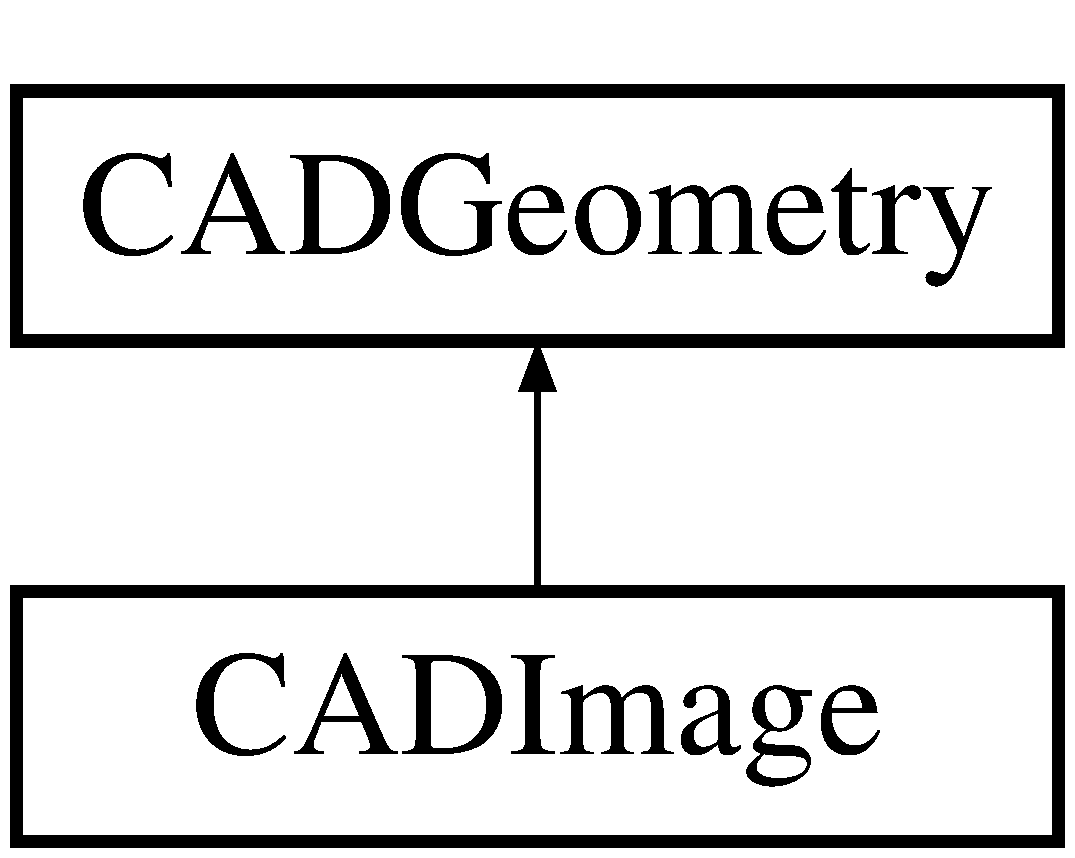
\includegraphics[height=2.000000cm]{class_c_a_d_image}
\end{center}
\end{figure}
\subsection*{Public Member Functions}
\begin{DoxyCompactItemize}
\item 
\hyperlink{class_c_a_d_vector}{C\+A\+D\+Vector} {\bfseries get\+Vert\+Insertion\+Point} () const \hypertarget{class_c_a_d_image_a0d801f1e4f26c493d30b77124c04d9e8}{}\label{class_c_a_d_image_a0d801f1e4f26c493d30b77124c04d9e8}

\item 
void {\bfseries set\+Vert\+Insertion\+Point} (const \hyperlink{class_c_a_d_vector}{C\+A\+D\+Vector} \&value)\hypertarget{class_c_a_d_image_ad44b9711c05eee17f0cfb0bb60f7970b}{}\label{class_c_a_d_image_ad44b9711c05eee17f0cfb0bb60f7970b}

\item 
\hyperlink{class_c_a_d_vector}{C\+A\+D\+Vector} {\bfseries get\+Image\+Size} () const \hypertarget{class_c_a_d_image_aaa76930e115facb70310199360786da4}{}\label{class_c_a_d_image_aaa76930e115facb70310199360786da4}

\item 
void {\bfseries set\+Image\+Size} (const \hyperlink{class_c_a_d_vector}{C\+A\+D\+Vector} \&value)\hypertarget{class_c_a_d_image_a806094956012bbfe4b3cd3123f1da75b}{}\label{class_c_a_d_image_a806094956012bbfe4b3cd3123f1da75b}

\item 
\hyperlink{class_c_a_d_vector}{C\+A\+D\+Vector} {\bfseries get\+Image\+Size\+In\+Px} () const \hypertarget{class_c_a_d_image_af111d15469ad9f41f85b8f7f39e22b82}{}\label{class_c_a_d_image_af111d15469ad9f41f85b8f7f39e22b82}

\item 
void {\bfseries set\+Image\+Size\+In\+Px} (const \hyperlink{class_c_a_d_vector}{C\+A\+D\+Vector} \&value)\hypertarget{class_c_a_d_image_a4b6631ac8973ed25f40e9b5369f068da}{}\label{class_c_a_d_image_a4b6631ac8973ed25f40e9b5369f068da}

\item 
\hyperlink{class_c_a_d_vector}{C\+A\+D\+Vector} {\bfseries get\+Pixel\+Size\+In\+A\+C\+A\+D\+Units} () const \hypertarget{class_c_a_d_image_afdaf3bfebbad316f6add46c64bea59e1}{}\label{class_c_a_d_image_afdaf3bfebbad316f6add46c64bea59e1}

\item 
void {\bfseries set\+Pixel\+Size\+In\+A\+C\+A\+D\+Units} (const \hyperlink{class_c_a_d_vector}{C\+A\+D\+Vector} \&value)\hypertarget{class_c_a_d_image_a1bc2f6b57b11ac1d7afd5f24cadbf4c7}{}\label{class_c_a_d_image_a1bc2f6b57b11ac1d7afd5f24cadbf4c7}

\item 
short {\bfseries get\+Clipping\+Boundary\+Type} () const \hypertarget{class_c_a_d_image_a577f2d1a9f5d65ce58b4967af3fbae69}{}\label{class_c_a_d_image_a577f2d1a9f5d65ce58b4967af3fbae69}

\item 
void {\bfseries set\+Clipping\+Boundary\+Type} (short value)\hypertarget{class_c_a_d_image_aa4cc4146fa6ca1bbdc32a777ffa061f1}{}\label{class_c_a_d_image_aa4cc4146fa6ca1bbdc32a777ffa061f1}

\item 
unsigned char {\bfseries get\+Resolution\+Units} () const \hypertarget{class_c_a_d_image_aac9e62121508ae4b1e9c68bd07218c49}{}\label{class_c_a_d_image_aac9e62121508ae4b1e9c68bd07218c49}

\item 
void {\bfseries set\+Resolution\+Units} (unsigned char value)\hypertarget{class_c_a_d_image_a42f06a2f48b78b741607ee6defa22642}{}\label{class_c_a_d_image_a42f06a2f48b78b741607ee6defa22642}

\item 
string {\bfseries get\+File\+Path} () const \hypertarget{class_c_a_d_image_aaac79b3c18e301c5d1ca24323bab4766}{}\label{class_c_a_d_image_aaac79b3c18e301c5d1ca24323bab4766}

\item 
void {\bfseries set\+File\+Path} (const string \&value)\hypertarget{class_c_a_d_image_af3a88e40c65175c089c1d5f2dee364c2}{}\label{class_c_a_d_image_af3a88e40c65175c089c1d5f2dee364c2}

\item 
void {\bfseries set\+Options} (bool transparency, bool clip, unsigned char brightness, unsigned char contrast)\hypertarget{class_c_a_d_image_af01bb204aaab3e84bd13e6be0f4aa602}{}\label{class_c_a_d_image_af01bb204aaab3e84bd13e6be0f4aa602}

\item 
virtual void {\bfseries print} () const  override\hypertarget{class_c_a_d_image_af05c090911108ad91b8edda1eeb0ce8f}{}\label{class_c_a_d_image_af05c090911108ad91b8edda1eeb0ce8f}

\item 
void {\bfseries add\+Clipping\+Point} (const \hyperlink{class_c_a_d_vector}{C\+A\+D\+Vector} \&pt)\hypertarget{class_c_a_d_image_a84331cc0502fde358bf4ccfc4725e9b1}{}\label{class_c_a_d_image_a84331cc0502fde358bf4ccfc4725e9b1}

\end{DoxyCompactItemize}
\subsection*{Protected Attributes}
\begin{DoxyCompactItemize}
\item 
\hyperlink{class_c_a_d_vector}{C\+A\+D\+Vector} {\bfseries vert\+Insertion\+Point}\hypertarget{class_c_a_d_image_a8829a273086dadedda0719d8d83a4904}{}\label{class_c_a_d_image_a8829a273086dadedda0719d8d83a4904}

\item 
\hyperlink{class_c_a_d_vector}{C\+A\+D\+Vector} {\bfseries image\+Size}\hypertarget{class_c_a_d_image_a87c6eb73a7b81fe28c8df3203553e547}{}\label{class_c_a_d_image_a87c6eb73a7b81fe28c8df3203553e547}

\item 
bool {\bfseries b\+Transparency}\hypertarget{class_c_a_d_image_a209d0125f3d725be201df93852a46e17}{}\label{class_c_a_d_image_a209d0125f3d725be201df93852a46e17}

\item 
bool {\bfseries b\+Clipping}\hypertarget{class_c_a_d_image_a44ba67554699da20f767f13b6a3a6214}{}\label{class_c_a_d_image_a44ba67554699da20f767f13b6a3a6214}

\item 
unsigned char {\bfseries d\+Brightness}\hypertarget{class_c_a_d_image_aee4ce055b1e5341c6da019485aa4c6e1}{}\label{class_c_a_d_image_aee4ce055b1e5341c6da019485aa4c6e1}

\item 
unsigned char {\bfseries d\+Contrast}\hypertarget{class_c_a_d_image_a78d8f337b278072db1c3c290bea6096c}{}\label{class_c_a_d_image_a78d8f337b278072db1c3c290bea6096c}

\item 
\hyperlink{class_c_a_d_vector}{C\+A\+D\+Vector} {\bfseries image\+Size\+In\+Px}\hypertarget{class_c_a_d_image_ad9b830757e767e508945a60b12d5269a}{}\label{class_c_a_d_image_ad9b830757e767e508945a60b12d5269a}

\item 
string {\bfseries file\+Path}\hypertarget{class_c_a_d_image_ad88a985c9f856e4c569c32e6a47e4ac6}{}\label{class_c_a_d_image_ad88a985c9f856e4c569c32e6a47e4ac6}

\item 
unsigned char {\bfseries resolution\+Units}\hypertarget{class_c_a_d_image_aac598b7bc4642ec14b5d20befb8108e7}{}\label{class_c_a_d_image_aac598b7bc4642ec14b5d20befb8108e7}

\item 
\hyperlink{class_c_a_d_vector}{C\+A\+D\+Vector} {\bfseries pixel\+Size\+In\+A\+C\+A\+D\+Units}\hypertarget{class_c_a_d_image_a963c7c65f866d1e7ca74b643d0104c3a}{}\label{class_c_a_d_image_a963c7c65f866d1e7ca74b643d0104c3a}

\item 
short {\bfseries clipping\+Boundary\+Type}\hypertarget{class_c_a_d_image_a5e74db472d61a9fc85aafdfe6d3dc798}{}\label{class_c_a_d_image_a5e74db472d61a9fc85aafdfe6d3dc798}

\item 
vector$<$ \hyperlink{class_c_a_d_vector}{C\+A\+D\+Vector} $>$ {\bfseries avert\+Clipping\+Polygon}\hypertarget{class_c_a_d_image_acbe02cefac39b90208d57a445e114dbc}{}\label{class_c_a_d_image_acbe02cefac39b90208d57a445e114dbc}

\end{DoxyCompactItemize}
\subsection*{Additional Inherited Members}


\subsection{Detailed Description}
Geometry class which represents Image (Raster Image) 

The documentation for this class was generated from the following files\+:\begin{DoxyCompactItemize}
\item 
cadgeometry.\+h\item 
cadgeometry.\+cpp\end{DoxyCompactItemize}

\hypertarget{class_c_a_d_image_def_object}{}\section{C\+A\+D\+Image\+Def\+Object Class Reference}
\label{class_c_a_d_image_def_object}\index{C\+A\+D\+Image\+Def\+Object@{C\+A\+D\+Image\+Def\+Object}}


The \hyperlink{class_c_a_d_image_def_object}{C\+A\+D\+Image\+Def\+Object} class.  




{\ttfamily \#include $<$cadobjects.\+h$>$}

Inheritance diagram for C\+A\+D\+Image\+Def\+Object\+:\begin{figure}[H]
\begin{center}
\leavevmode
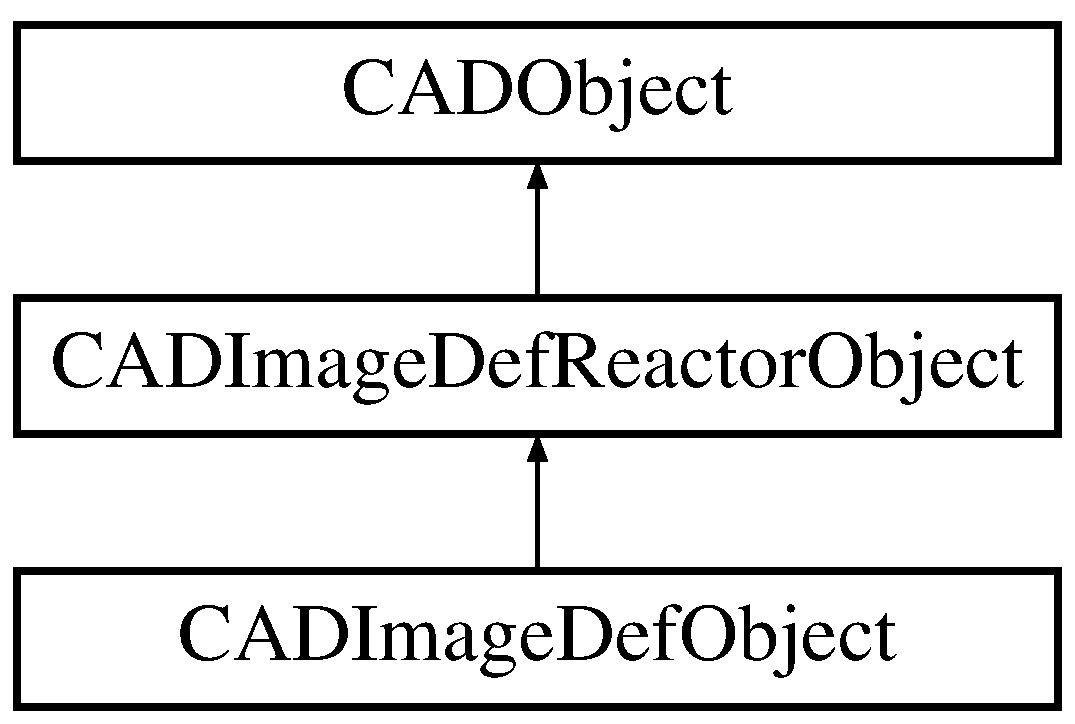
\includegraphics[height=3.000000cm]{class_c_a_d_image_def_object}
\end{center}
\end{figure}
\subsection*{Public Attributes}
\begin{DoxyCompactItemize}
\item 
double {\bfseries df\+X\+Image\+Size\+In\+Px}\hypertarget{class_c_a_d_image_def_object_ad2e39e446e37152ebf60fb1e8ad97fe2}{}\label{class_c_a_d_image_def_object_ad2e39e446e37152ebf60fb1e8ad97fe2}

\item 
double {\bfseries df\+Y\+Image\+Size\+In\+Px}\hypertarget{class_c_a_d_image_def_object_a0c6669b0799ca8a4e8249917dcb9724c}{}\label{class_c_a_d_image_def_object_a0c6669b0799ca8a4e8249917dcb9724c}

\item 
string {\bfseries s\+File\+Path}\hypertarget{class_c_a_d_image_def_object_a088debaa7a45fe9347d9a2490d7d7021}{}\label{class_c_a_d_image_def_object_a088debaa7a45fe9347d9a2490d7d7021}

\item 
bool {\bfseries b\+Is\+Loaded}\hypertarget{class_c_a_d_image_def_object_a6753acf3bc670a2990fd540885e79097}{}\label{class_c_a_d_image_def_object_a6753acf3bc670a2990fd540885e79097}

\item 
unsigned char {\bfseries d\+Res\+Units}\hypertarget{class_c_a_d_image_def_object_aa8d71f2c8d4ae62d7196d8e44c658995}{}\label{class_c_a_d_image_def_object_aa8d71f2c8d4ae62d7196d8e44c658995}

\item 
double {\bfseries df\+X\+Pixel\+Size}\hypertarget{class_c_a_d_image_def_object_aad8ae5aa83ac9b4d71ddb0551a1a98c2}{}\label{class_c_a_d_image_def_object_aad8ae5aa83ac9b4d71ddb0551a1a98c2}

\item 
double {\bfseries df\+Y\+Pixel\+Size}\hypertarget{class_c_a_d_image_def_object_aeed242209d59504dc5733a2df734104c}{}\label{class_c_a_d_image_def_object_aeed242209d59504dc5733a2df734104c}

\end{DoxyCompactItemize}
\subsection*{Additional Inherited Members}


\subsection{Detailed Description}
The \hyperlink{class_c_a_d_image_def_object}{C\+A\+D\+Image\+Def\+Object} class. 

The documentation for this class was generated from the following files\+:\begin{DoxyCompactItemize}
\item 
cadobjects.\+h\item 
cadobjects.\+cpp\end{DoxyCompactItemize}

\hypertarget{class_c_a_d_image_def_reactor_object}{}\section{C\+A\+D\+Image\+Def\+Reactor\+Object Class Reference}
\label{class_c_a_d_image_def_reactor_object}\index{C\+A\+D\+Image\+Def\+Reactor\+Object@{C\+A\+D\+Image\+Def\+Reactor\+Object}}


The \hyperlink{class_c_a_d_image_def_reactor_object}{C\+A\+D\+Image\+Def\+Reactor\+Object} class.  




{\ttfamily \#include $<$cadobjects.\+h$>$}

Inheritance diagram for C\+A\+D\+Image\+Def\+Reactor\+Object\+:\begin{figure}[H]
\begin{center}
\leavevmode
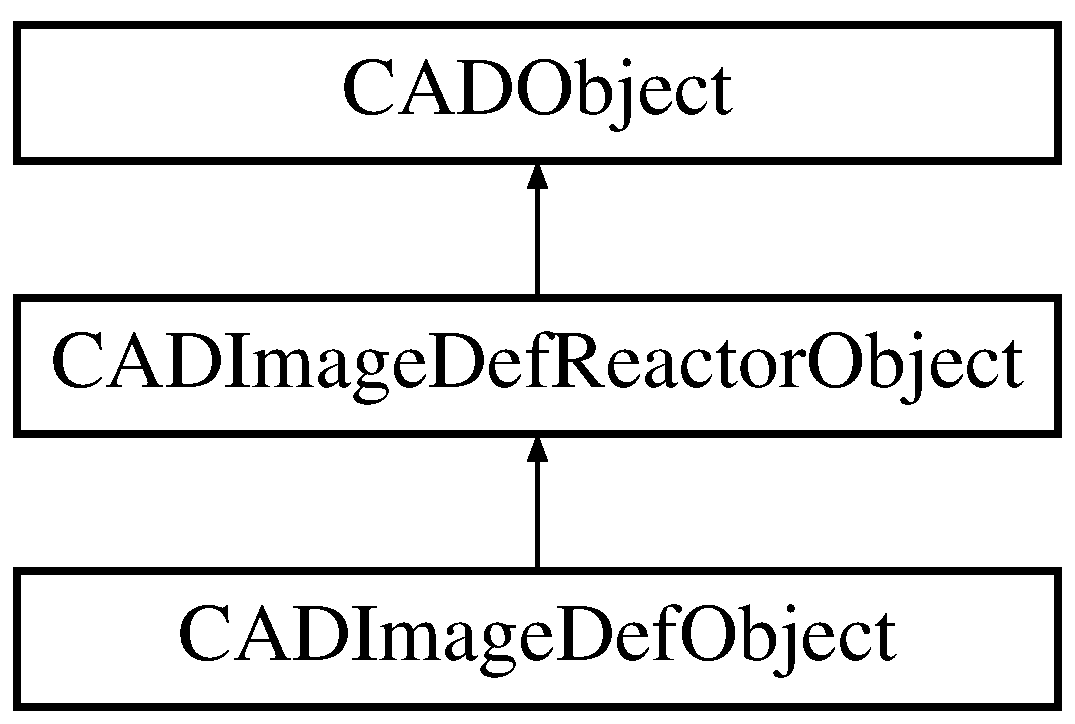
\includegraphics[height=3.000000cm]{class_c_a_d_image_def_reactor_object}
\end{center}
\end{figure}
\subsection*{Public Attributes}
\begin{DoxyCompactItemize}
\item 
long {\bfseries n\+Object\+Size\+In\+Bits}\hypertarget{class_c_a_d_image_def_reactor_object_acaface5db904c1f5d27a022298b93fc0}{}\label{class_c_a_d_image_def_reactor_object_acaface5db904c1f5d27a022298b93fc0}

\item 
\hyperlink{class_c_a_d_handle}{C\+A\+D\+Handle} {\bfseries h\+Object\+Handle}\hypertarget{class_c_a_d_image_def_reactor_object_a2b43d9dd753c71322957a0d0254575bb}{}\label{class_c_a_d_image_def_reactor_object_a2b43d9dd753c71322957a0d0254575bb}

\item 
vector$<$ \hyperlink{struct___eed}{C\+A\+D\+Eed} $>$ {\bfseries a\+E\+ED}\hypertarget{class_c_a_d_image_def_reactor_object_a1a068859878629e83437850efcb46166}{}\label{class_c_a_d_image_def_reactor_object_a1a068859878629e83437850efcb46166}

\item 
long {\bfseries n\+Num\+Reactors}\hypertarget{class_c_a_d_image_def_reactor_object_a20fb128173c4d8894f672c15ca42a8d5}{}\label{class_c_a_d_image_def_reactor_object_a20fb128173c4d8894f672c15ca42a8d5}

\item 
bool {\bfseries b\+No\+X\+Dictionary\+Present}\hypertarget{class_c_a_d_image_def_reactor_object_a20e2a3292c03e8b0b8325d0b8805cd89}{}\label{class_c_a_d_image_def_reactor_object_a20e2a3292c03e8b0b8325d0b8805cd89}

\item 
long {\bfseries d\+Class\+Version}\hypertarget{class_c_a_d_image_def_reactor_object_a40ede90d113ce0e102bb1d164b7ba1f7}{}\label{class_c_a_d_image_def_reactor_object_a40ede90d113ce0e102bb1d164b7ba1f7}

\item 
\hyperlink{class_c_a_d_handle}{C\+A\+D\+Handle} {\bfseries h\+Parent\+Handle}\hypertarget{class_c_a_d_image_def_reactor_object_ac1a7b75364b35285bda3f07819c93abe}{}\label{class_c_a_d_image_def_reactor_object_ac1a7b75364b35285bda3f07819c93abe}

\item 
vector$<$ \hyperlink{class_c_a_d_handle}{C\+A\+D\+Handle} $>$ {\bfseries h\+Reactors}\hypertarget{class_c_a_d_image_def_reactor_object_a9e2cc5ecf8ca7d3911df68ec107460fa}{}\label{class_c_a_d_image_def_reactor_object_a9e2cc5ecf8ca7d3911df68ec107460fa}

\item 
\hyperlink{class_c_a_d_handle}{C\+A\+D\+Handle} {\bfseries h\+X\+Dictionary}\hypertarget{class_c_a_d_image_def_reactor_object_abf637cad59b9049ad6bde4e58bbe8ac0}{}\label{class_c_a_d_image_def_reactor_object_abf637cad59b9049ad6bde4e58bbe8ac0}

\end{DoxyCompactItemize}
\subsection*{Additional Inherited Members}


\subsection{Detailed Description}
The \hyperlink{class_c_a_d_image_def_reactor_object}{C\+A\+D\+Image\+Def\+Reactor\+Object} class. 

The documentation for this class was generated from the following files\+:\begin{DoxyCompactItemize}
\item 
cadobjects.\+h\item 
cadobjects.\+cpp\end{DoxyCompactItemize}

\hypertarget{class_c_a_d_image_object}{}\section{C\+A\+D\+Image\+Object Class Reference}
\label{class_c_a_d_image_object}\index{C\+A\+D\+Image\+Object@{C\+A\+D\+Image\+Object}}


The \hyperlink{class_c_a_d_image_object}{C\+A\+D\+Image\+Object} class.  




{\ttfamily \#include $<$cadobjects.\+h$>$}

Inheritance diagram for C\+A\+D\+Image\+Object\+:\begin{figure}[H]
\begin{center}
\leavevmode
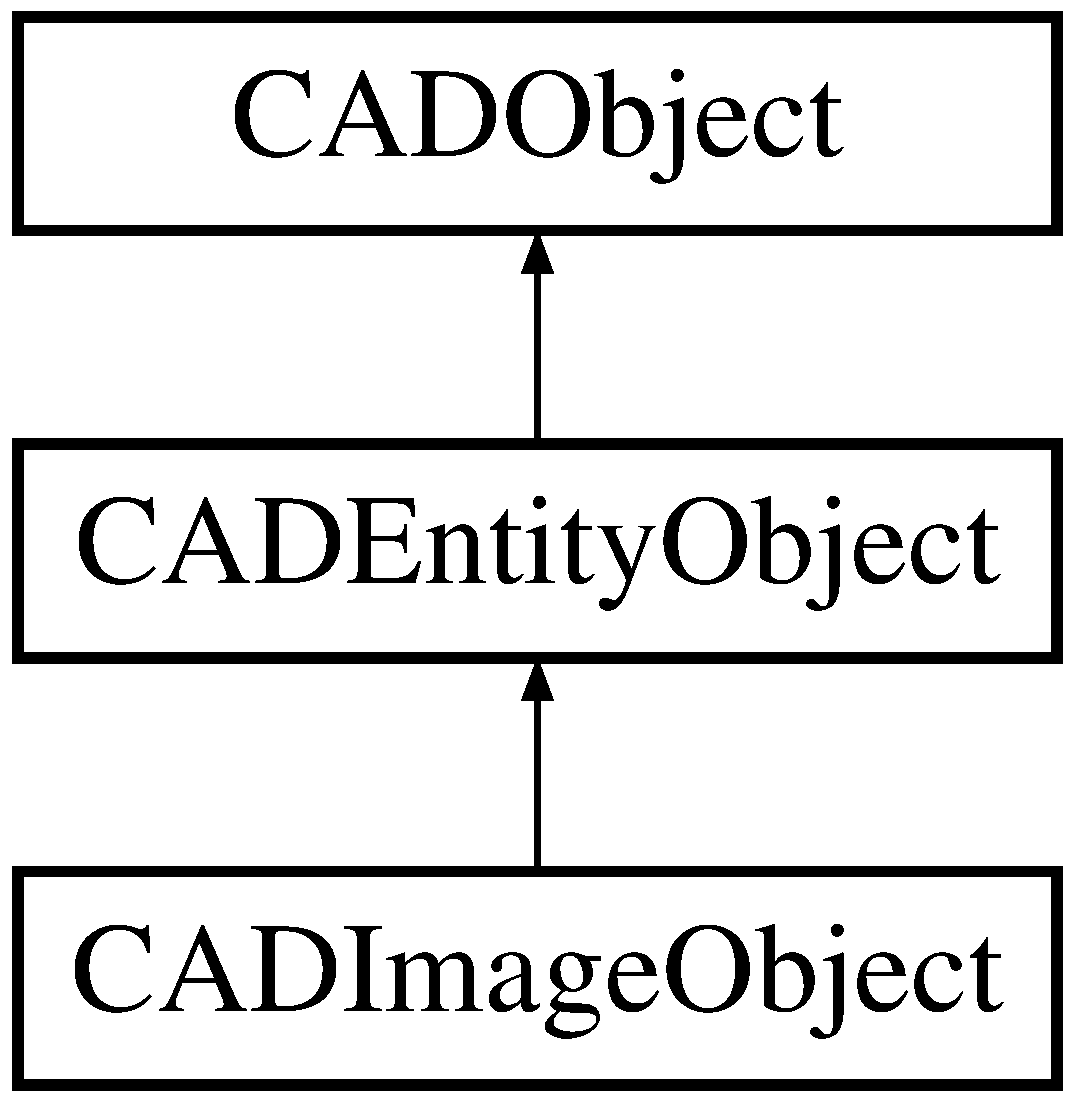
\includegraphics[height=3.000000cm]{class_c_a_d_image_object}
\end{center}
\end{figure}
\subsection*{Public Attributes}
\begin{DoxyCompactItemize}
\item 
long {\bfseries d\+Class\+Version}\hypertarget{class_c_a_d_image_object_a94e8f50b231b3d2ee81fc6e079484471}{}\label{class_c_a_d_image_object_a94e8f50b231b3d2ee81fc6e079484471}

\item 
\hyperlink{class_c_a_d_vector}{C\+A\+D\+Vector} {\bfseries vert\+Insertion}\hypertarget{class_c_a_d_image_object_afd3cb1292aebb39e8bb8a078aaa3bf61}{}\label{class_c_a_d_image_object_afd3cb1292aebb39e8bb8a078aaa3bf61}

\item 
\hyperlink{class_c_a_d_vector}{C\+A\+D\+Vector} {\bfseries vect\+U\+Direction}\hypertarget{class_c_a_d_image_object_aeca11d6b109297590e0e0ed429620f62}{}\label{class_c_a_d_image_object_aeca11d6b109297590e0e0ed429620f62}

\item 
\hyperlink{class_c_a_d_vector}{C\+A\+D\+Vector} {\bfseries vect\+V\+Direction}\hypertarget{class_c_a_d_image_object_a6bc69f08ee275ceed83d237cf2e421c1}{}\label{class_c_a_d_image_object_a6bc69f08ee275ceed83d237cf2e421c1}

\item 
double {\bfseries df\+SizeX}\hypertarget{class_c_a_d_image_object_aa3dd7b20082f43cc5bf690874e044622}{}\label{class_c_a_d_image_object_aa3dd7b20082f43cc5bf690874e044622}

\item 
double {\bfseries df\+SizeY}\hypertarget{class_c_a_d_image_object_a052de3595cadc838d076c665bc4a43ba}{}\label{class_c_a_d_image_object_a052de3595cadc838d076c665bc4a43ba}

\item 
short {\bfseries d\+Display\+Props}\hypertarget{class_c_a_d_image_object_a857e5fb5a5819326f6f37f643721c8dc}{}\label{class_c_a_d_image_object_a857e5fb5a5819326f6f37f643721c8dc}

\item 
bool {\bfseries b\+Clipping}\hypertarget{class_c_a_d_image_object_a9d09904df634543f9d8ff6f419a6db9e}{}\label{class_c_a_d_image_object_a9d09904df634543f9d8ff6f419a6db9e}

\item 
unsigned char {\bfseries d\+Brightness}\hypertarget{class_c_a_d_image_object_ac97ddbf8c28b35020107189d57e60ffb}{}\label{class_c_a_d_image_object_ac97ddbf8c28b35020107189d57e60ffb}

\item 
unsigned char {\bfseries d\+Contrast}\hypertarget{class_c_a_d_image_object_ab3f4b2371ffa715c3f565dd29c7f38dc}{}\label{class_c_a_d_image_object_ab3f4b2371ffa715c3f565dd29c7f38dc}

\item 
unsigned char {\bfseries d\+Fade}\hypertarget{class_c_a_d_image_object_a9c7fb3e6570d198afb12e5e5877decb4}{}\label{class_c_a_d_image_object_a9c7fb3e6570d198afb12e5e5877decb4}

\item 
bool {\bfseries b\+Clip\+Mode}\hypertarget{class_c_a_d_image_object_a5ac504ec0ca34bb5ea3cd612b1f3b26b}{}\label{class_c_a_d_image_object_a5ac504ec0ca34bb5ea3cd612b1f3b26b}

\item 
short {\bfseries d\+Clip\+Boundary\+Type}\hypertarget{class_c_a_d_image_object_aaeec845db48525fc12324aefe904cfe2}{}\label{class_c_a_d_image_object_aaeec845db48525fc12324aefe904cfe2}

\item 
long {\bfseries n\+Number\+Vertexes\+In\+Clip\+Polygon}\hypertarget{class_c_a_d_image_object_a35f965686c72c7a294f754b1deb31482}{}\label{class_c_a_d_image_object_a35f965686c72c7a294f754b1deb31482}

\item 
vector$<$ \hyperlink{class_c_a_d_vector}{C\+A\+D\+Vector} $>$ {\bfseries avert\+Clipping\+Polygon\+Vertexes}\hypertarget{class_c_a_d_image_object_a46547fa998ac3705c768bf68ba5f1eaf}{}\label{class_c_a_d_image_object_a46547fa998ac3705c768bf68ba5f1eaf}

\item 
\hyperlink{class_c_a_d_handle}{C\+A\+D\+Handle} {\bfseries h\+Image\+Def}\hypertarget{class_c_a_d_image_object_a93000fa9564f5367a7cde0d84968b066}{}\label{class_c_a_d_image_object_a93000fa9564f5367a7cde0d84968b066}

\item 
\hyperlink{class_c_a_d_handle}{C\+A\+D\+Handle} {\bfseries h\+Image\+Def\+Reactor}\hypertarget{class_c_a_d_image_object_aedd9ca1c46af776a185370b395af5516}{}\label{class_c_a_d_image_object_aedd9ca1c46af776a185370b395af5516}

\end{DoxyCompactItemize}
\subsection*{Additional Inherited Members}


\subsection{Detailed Description}
The \hyperlink{class_c_a_d_image_object}{C\+A\+D\+Image\+Object} class. 

The documentation for this class was generated from the following files\+:\begin{DoxyCompactItemize}
\item 
cadobjects.\+h\item 
cadobjects.\+cpp\end{DoxyCompactItemize}

\hypertarget{class_c_a_d_insert_object}{}\section{C\+A\+D\+Insert\+Object Class Reference}
\label{class_c_a_d_insert_object}\index{C\+A\+D\+Insert\+Object@{C\+A\+D\+Insert\+Object}}


The \hyperlink{class_c_a_d_insert_object}{C\+A\+D\+Insert\+Object} class.  




{\ttfamily \#include $<$cadobjects.\+h$>$}

Inheritance diagram for C\+A\+D\+Insert\+Object\+:\begin{figure}[H]
\begin{center}
\leavevmode
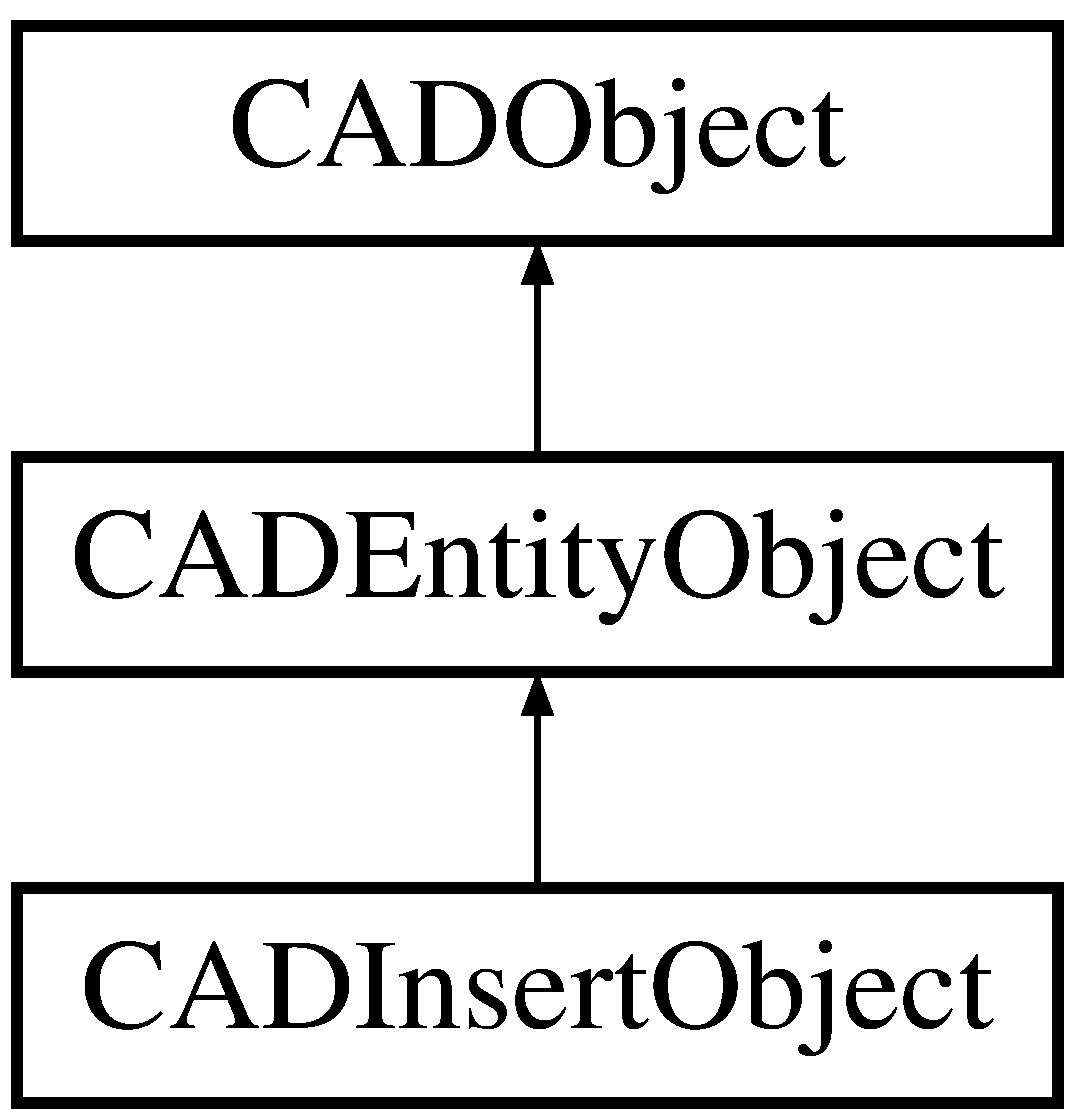
\includegraphics[height=3.000000cm]{class_c_a_d_insert_object}
\end{center}
\end{figure}
\subsection*{Public Attributes}
\begin{DoxyCompactItemize}
\item 
\hyperlink{class_c_a_d_vector}{C\+A\+D\+Vector} {\bfseries vert\+Insertion\+Point}\hypertarget{class_c_a_d_insert_object_a580400ba7ed3620012987258ca7724d6}{}\label{class_c_a_d_insert_object_a580400ba7ed3620012987258ca7724d6}

\item 
\hyperlink{class_c_a_d_vector}{C\+A\+D\+Vector} {\bfseries vert\+Scales}\hypertarget{class_c_a_d_insert_object_a850289fd8022a5df6be821ad173f971b}{}\label{class_c_a_d_insert_object_a850289fd8022a5df6be821ad173f971b}

\item 
double {\bfseries df\+Rotation}\hypertarget{class_c_a_d_insert_object_acffd6449c59ab915ec397a5a5d1e5619}{}\label{class_c_a_d_insert_object_acffd6449c59ab915ec397a5a5d1e5619}

\item 
\hyperlink{class_c_a_d_vector}{C\+A\+D\+Vector} {\bfseries vect\+Extrusion}\hypertarget{class_c_a_d_insert_object_afff3fd1818c92a7e07cbc2b1c3421892}{}\label{class_c_a_d_insert_object_afff3fd1818c92a7e07cbc2b1c3421892}

\item 
bool {\bfseries b\+Has\+Attribs}\hypertarget{class_c_a_d_insert_object_a7b39ba59c276e40f106aed9dce95d561}{}\label{class_c_a_d_insert_object_a7b39ba59c276e40f106aed9dce95d561}

\item 
long {\bfseries n\+Objects\+Owned}\hypertarget{class_c_a_d_insert_object_a19b2b8e8d7732ac86771f8ac07a6eb95}{}\label{class_c_a_d_insert_object_a19b2b8e8d7732ac86771f8ac07a6eb95}

\item 
\hyperlink{class_c_a_d_handle}{C\+A\+D\+Handle} {\bfseries h\+Block\+Header}\hypertarget{class_c_a_d_insert_object_a79f7eee43b80f83b4b5d9431ee523bc4}{}\label{class_c_a_d_insert_object_a79f7eee43b80f83b4b5d9431ee523bc4}

\item 
C\+A\+D\+Handle\+Array {\bfseries h\+Atrribs}\hypertarget{class_c_a_d_insert_object_a03674f62c1b2a216f3df6dc0e1865142}{}\label{class_c_a_d_insert_object_a03674f62c1b2a216f3df6dc0e1865142}

\item 
\hyperlink{class_c_a_d_handle}{C\+A\+D\+Handle} {\bfseries h\+Seqend}\hypertarget{class_c_a_d_insert_object_a3e1a4ba09ea06c2a8584704f9dea6a07}{}\label{class_c_a_d_insert_object_a3e1a4ba09ea06c2a8584704f9dea6a07}

\end{DoxyCompactItemize}
\subsection*{Additional Inherited Members}


\subsection{Detailed Description}
The \hyperlink{class_c_a_d_insert_object}{C\+A\+D\+Insert\+Object} class. 

The documentation for this class was generated from the following files\+:\begin{DoxyCompactItemize}
\item 
cadobjects.\+h\item 
cadobjects.\+cpp\end{DoxyCompactItemize}

\hypertarget{class_c_a_d_layer}{}\section{C\+A\+D\+Layer Class Reference}
\label{class_c_a_d_layer}\index{C\+A\+D\+Layer@{C\+A\+D\+Layer}}
\subsection*{Public Member Functions}
\begin{DoxyCompactItemize}
\item 
{\bfseries C\+A\+D\+Layer} (\hyperlink{class_c_a_d_file}{C\+A\+D\+File} $\ast$const file)\hypertarget{class_c_a_d_layer_aa6d8888ff1c36c9eb81000448e829e9c}{}\label{class_c_a_d_layer_aa6d8888ff1c36c9eb81000448e829e9c}

\item 
string {\bfseries get\+Name} () const \hypertarget{class_c_a_d_layer_aaf7093bc3420a5b32fba2952d71a560b}{}\label{class_c_a_d_layer_aaf7093bc3420a5b32fba2952d71a560b}

\item 
void {\bfseries set\+Name} (const string \&value)\hypertarget{class_c_a_d_layer_a604998bc6878ec32f512b2231b8c59ff}{}\label{class_c_a_d_layer_a604998bc6878ec32f512b2231b8c59ff}

\item 
bool {\bfseries get\+Frozen} () const \hypertarget{class_c_a_d_layer_accd955ff448032d00f5e7eeacf29ecbd}{}\label{class_c_a_d_layer_accd955ff448032d00f5e7eeacf29ecbd}

\item 
void {\bfseries set\+Frozen} (bool value)\hypertarget{class_c_a_d_layer_aa3fd384bd46ff0ae99758c28d18a0404}{}\label{class_c_a_d_layer_aa3fd384bd46ff0ae99758c28d18a0404}

\item 
bool {\bfseries get\+On} () const \hypertarget{class_c_a_d_layer_a62609972d7388381e0a7ef7a16e6e462}{}\label{class_c_a_d_layer_a62609972d7388381e0a7ef7a16e6e462}

\item 
void {\bfseries set\+On} (bool value)\hypertarget{class_c_a_d_layer_a62238a4b8ee55db8d2433676ba7e8d72}{}\label{class_c_a_d_layer_a62238a4b8ee55db8d2433676ba7e8d72}

\item 
bool {\bfseries get\+Frozen\+By\+Default} () const \hypertarget{class_c_a_d_layer_ad9a5b8eedf99a44eea36d73f88dc4270}{}\label{class_c_a_d_layer_ad9a5b8eedf99a44eea36d73f88dc4270}

\item 
void {\bfseries set\+Frozen\+By\+Default} (bool value)\hypertarget{class_c_a_d_layer_ace144c9fc2c59a198738cc65dc12c119}{}\label{class_c_a_d_layer_ace144c9fc2c59a198738cc65dc12c119}

\item 
bool {\bfseries get\+Locked} () const \hypertarget{class_c_a_d_layer_a47dfb61064763179050e7c99d1a2a2d7}{}\label{class_c_a_d_layer_a47dfb61064763179050e7c99d1a2a2d7}

\item 
void {\bfseries set\+Locked} (bool value)\hypertarget{class_c_a_d_layer_a5e893f778234b07cef2f897f009c774a}{}\label{class_c_a_d_layer_a5e893f778234b07cef2f897f009c774a}

\item 
bool {\bfseries get\+Plotting} () const \hypertarget{class_c_a_d_layer_ae572fcdb395fe585a5e7f767889e015b}{}\label{class_c_a_d_layer_ae572fcdb395fe585a5e7f767889e015b}

\item 
void {\bfseries set\+Plotting} (bool value)\hypertarget{class_c_a_d_layer_a286e918371dea97c696892c01c08dd97}{}\label{class_c_a_d_layer_a286e918371dea97c696892c01c08dd97}

\item 
short {\bfseries get\+Line\+Weight} () const \hypertarget{class_c_a_d_layer_a65c5a10007fe65362159531546b31fdc}{}\label{class_c_a_d_layer_a65c5a10007fe65362159531546b31fdc}

\item 
void {\bfseries set\+Line\+Weight} (short value)\hypertarget{class_c_a_d_layer_ab3f59ef7f14a88e85d7adf540074b811}{}\label{class_c_a_d_layer_ab3f59ef7f14a88e85d7adf540074b811}

\item 
short {\bfseries get\+Color} () const \hypertarget{class_c_a_d_layer_a6900a8f0a5a35e8b557ca26b478ff31c}{}\label{class_c_a_d_layer_a6900a8f0a5a35e8b557ca26b478ff31c}

\item 
void {\bfseries set\+Color} (short value)\hypertarget{class_c_a_d_layer_a2ff76d08d34007d0f665847fbfc61370}{}\label{class_c_a_d_layer_a2ff76d08d34007d0f665847fbfc61370}

\item 
size\+\_\+t {\bfseries get\+Id} () const \hypertarget{class_c_a_d_layer_a3034c92c58baf41dfb322f2d650a97d4}{}\label{class_c_a_d_layer_a3034c92c58baf41dfb322f2d650a97d4}

\item 
void {\bfseries set\+Id} (const size\+\_\+t \&value)\hypertarget{class_c_a_d_layer_ac2af17d2ca4cd847cb573b69bc5b8ba6}{}\label{class_c_a_d_layer_ac2af17d2ca4cd847cb573b69bc5b8ba6}

\item 
long {\bfseries get\+Handle} () const \hypertarget{class_c_a_d_layer_a722ee842245d3d14260ea5954b374cdc}{}\label{class_c_a_d_layer_a722ee842245d3d14260ea5954b374cdc}

\item 
void {\bfseries set\+Handle} (long value)\hypertarget{class_c_a_d_layer_ad6fa1ac32929cadc4d5775e81891c0fc}{}\label{class_c_a_d_layer_ad6fa1ac32929cadc4d5775e81891c0fc}

\item 
void {\bfseries add\+Handle} (long handle, enum C\+A\+D\+Object\+::\+Object\+Type type)\hypertarget{class_c_a_d_layer_a931ddd3cd28216a52e2bf6c7c7ff6934}{}\label{class_c_a_d_layer_a931ddd3cd28216a52e2bf6c7c7ff6934}

\item 
size\+\_\+t {\bfseries get\+Geometry\+Count} () const \hypertarget{class_c_a_d_layer_acbd810558db7d327af19ba9b8b5eeff2}{}\label{class_c_a_d_layer_acbd810558db7d327af19ba9b8b5eeff2}

\item 
\hyperlink{class_c_a_d_geometry}{C\+A\+D\+Geometry} $\ast$ {\bfseries get\+Geometry} (size\+\_\+t index)\hypertarget{class_c_a_d_layer_a282ac6a605ceac97641c91eab6362df1}{}\label{class_c_a_d_layer_a282ac6a605ceac97641c91eab6362df1}

\end{DoxyCompactItemize}
\subsection*{Protected Attributes}
\begin{DoxyCompactItemize}
\item 
string {\bfseries layer\+Name}\hypertarget{class_c_a_d_layer_a1ca037d0494ca5bf871575645b19bc7f}{}\label{class_c_a_d_layer_a1ca037d0494ca5bf871575645b19bc7f}

\item 
bool {\bfseries frozen}\hypertarget{class_c_a_d_layer_a4be76412201399c311eb3842dee5b99e}{}\label{class_c_a_d_layer_a4be76412201399c311eb3842dee5b99e}

\item 
bool {\bfseries on}\hypertarget{class_c_a_d_layer_a811dd75742f5a84f666236a17903b97e}{}\label{class_c_a_d_layer_a811dd75742f5a84f666236a17903b97e}

\item 
bool {\bfseries frozen\+By\+Default}\hypertarget{class_c_a_d_layer_ad513c9301590ed4f12d64094f1213368}{}\label{class_c_a_d_layer_ad513c9301590ed4f12d64094f1213368}

\item 
bool {\bfseries locked}\hypertarget{class_c_a_d_layer_a222a521d790ff5a0cfa9c22cd6b775ae}{}\label{class_c_a_d_layer_a222a521d790ff5a0cfa9c22cd6b775ae}

\item 
bool {\bfseries plotting}\hypertarget{class_c_a_d_layer_afcf6ee15dcb0fa5c99d755dea4916e24}{}\label{class_c_a_d_layer_afcf6ee15dcb0fa5c99d755dea4916e24}

\item 
short {\bfseries line\+Weight}\hypertarget{class_c_a_d_layer_aa45be9da6742e65150cbc6c823a708f9}{}\label{class_c_a_d_layer_aa45be9da6742e65150cbc6c823a708f9}

\item 
short {\bfseries color}\hypertarget{class_c_a_d_layer_a2447a3bfaf004a45103b71074f30c6d4}{}\label{class_c_a_d_layer_a2447a3bfaf004a45103b71074f30c6d4}

\item 
size\+\_\+t {\bfseries layer\+Id}\hypertarget{class_c_a_d_layer_a1b6ed63d44cc22ff579e5b8e91d45438}{}\label{class_c_a_d_layer_a1b6ed63d44cc22ff579e5b8e91d45438}

\item 
long {\bfseries handle}\hypertarget{class_c_a_d_layer_a98aaf47433d4a761d50cb969f414a25e}{}\label{class_c_a_d_layer_a98aaf47433d4a761d50cb969f414a25e}

\item 
short {\bfseries geometry\+Type}\hypertarget{class_c_a_d_layer_a3d9b70a9eb88b5cf23011b58077d1951}{}\label{class_c_a_d_layer_a3d9b70a9eb88b5cf23011b58077d1951}

\item 
vector$<$ long $>$ {\bfseries geometry\+Handles}\hypertarget{class_c_a_d_layer_adee3d1116628797ae976f57fb1b874f4}{}\label{class_c_a_d_layer_adee3d1116628797ae976f57fb1b874f4}

\item 
vector$<$ long $>$ {\bfseries attribute\+Handles}\hypertarget{class_c_a_d_layer_ad9fb5d0e8710b2f6bf4554c4da6f013b}{}\label{class_c_a_d_layer_ad9fb5d0e8710b2f6bf4554c4da6f013b}

\item 
\hyperlink{class_c_a_d_file}{C\+A\+D\+File} $\ast$const {\bfseries p\+C\+A\+D\+File}\hypertarget{class_c_a_d_layer_aae8a4ce8ab88ce7263dc2d483e8e9253}{}\label{class_c_a_d_layer_aae8a4ce8ab88ce7263dc2d483e8e9253}

\end{DoxyCompactItemize}


The documentation for this class was generated from the following files\+:\begin{DoxyCompactItemize}
\item 
cadlayer.\+h\item 
cadlayer.\+cpp\end{DoxyCompactItemize}

\hypertarget{class_c_a_d_layer_control_object}{}\section{C\+A\+D\+Layer\+Control\+Object Class Reference}
\label{class_c_a_d_layer_control_object}\index{C\+A\+D\+Layer\+Control\+Object@{C\+A\+D\+Layer\+Control\+Object}}


The \hyperlink{class_c_a_d_layer_control_object}{C\+A\+D\+Layer\+Control\+Object} class.  




{\ttfamily \#include $<$cadobjects.\+h$>$}

Inheritance diagram for C\+A\+D\+Layer\+Control\+Object\+:\begin{figure}[H]
\begin{center}
\leavevmode
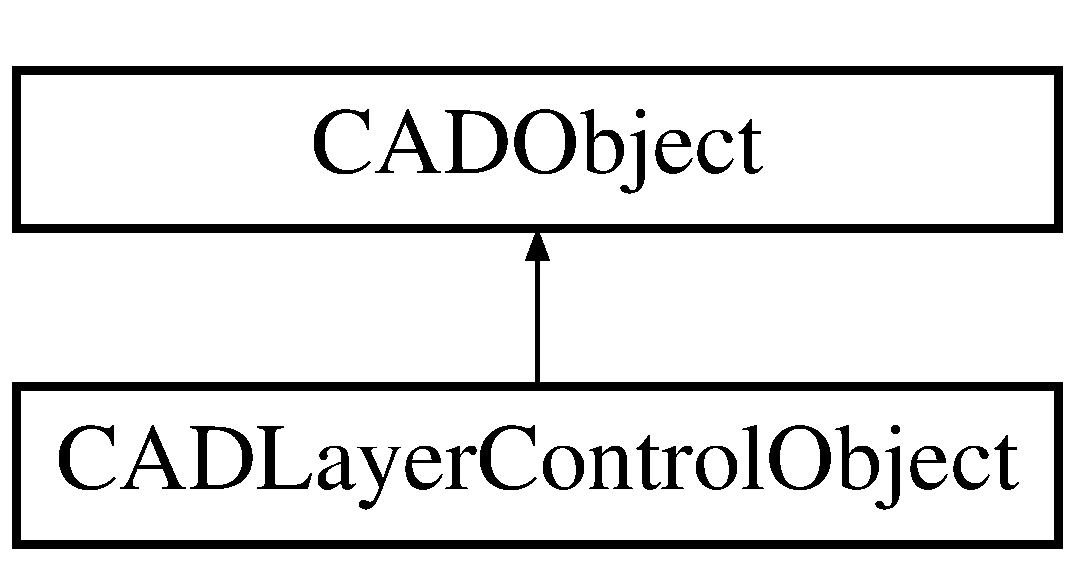
\includegraphics[height=2.000000cm]{class_c_a_d_layer_control_object}
\end{center}
\end{figure}
\subsection*{Public Attributes}
\begin{DoxyCompactItemize}
\item 
long {\bfseries n\+Object\+Size\+In\+Bits}\hypertarget{class_c_a_d_layer_control_object_afb2e02aafabe7f7b549f64853f52b416}{}\label{class_c_a_d_layer_control_object_afb2e02aafabe7f7b549f64853f52b416}

\item 
\hyperlink{class_c_a_d_handle}{C\+A\+D\+Handle} {\bfseries h\+Object\+Handle}\hypertarget{class_c_a_d_layer_control_object_a5a134909ac4c12e1f3eabafea74f0b1d}{}\label{class_c_a_d_layer_control_object_a5a134909ac4c12e1f3eabafea74f0b1d}

\item 
C\+A\+D\+Eed\+Array {\bfseries a\+E\+ED}\hypertarget{class_c_a_d_layer_control_object_a08168795b97556929a8aa72f716a90a2}{}\label{class_c_a_d_layer_control_object_a08168795b97556929a8aa72f716a90a2}

\item 
long {\bfseries n\+Num\+Reactors}\hypertarget{class_c_a_d_layer_control_object_a356e250d33be5a812c52eb594fd8a2ad}{}\label{class_c_a_d_layer_control_object_a356e250d33be5a812c52eb594fd8a2ad}

\item 
bool {\bfseries b\+No\+X\+Dictionary\+Present}\hypertarget{class_c_a_d_layer_control_object_a63b07e5ccc70dc0c1f56d516e3fb77f3}{}\label{class_c_a_d_layer_control_object_a63b07e5ccc70dc0c1f56d516e3fb77f3}

\item 
long {\bfseries n\+Num\+Entries}\hypertarget{class_c_a_d_layer_control_object_abf0c22f5948f223c5d4607d9048e5d93}{}\label{class_c_a_d_layer_control_object_abf0c22f5948f223c5d4607d9048e5d93}

\item 
\hyperlink{class_c_a_d_handle}{C\+A\+D\+Handle} {\bfseries h\+Null}\hypertarget{class_c_a_d_layer_control_object_ad0eeb86e3dfceec7e0e28d202e1266fd}{}\label{class_c_a_d_layer_control_object_ad0eeb86e3dfceec7e0e28d202e1266fd}

\item 
\hyperlink{class_c_a_d_handle}{C\+A\+D\+Handle} {\bfseries h\+X\+Dictionary}\hypertarget{class_c_a_d_layer_control_object_ad4ea38f1bbc5d0ff49cf00c817ecb89b}{}\label{class_c_a_d_layer_control_object_ad4ea38f1bbc5d0ff49cf00c817ecb89b}

\item 
C\+A\+D\+Handle\+Array {\bfseries h\+Layers}\hypertarget{class_c_a_d_layer_control_object_a832eb7cc78b6092eefb44ccff807a172}{}\label{class_c_a_d_layer_control_object_a832eb7cc78b6092eefb44ccff807a172}

\end{DoxyCompactItemize}
\subsection*{Additional Inherited Members}


\subsection{Detailed Description}
The \hyperlink{class_c_a_d_layer_control_object}{C\+A\+D\+Layer\+Control\+Object} class. 

The documentation for this class was generated from the following files\+:\begin{DoxyCompactItemize}
\item 
cadobjects.\+h\item 
cadobjects.\+cpp\end{DoxyCompactItemize}

\hypertarget{class_c_a_d_layer_object}{}\section{C\+A\+D\+Layer\+Object Class Reference}
\label{class_c_a_d_layer_object}\index{C\+A\+D\+Layer\+Object@{C\+A\+D\+Layer\+Object}}


The \hyperlink{class_c_a_d_layer_object}{C\+A\+D\+Layer\+Object} class.  




{\ttfamily \#include $<$cadobjects.\+h$>$}

Inheritance diagram for C\+A\+D\+Layer\+Object\+:\begin{figure}[H]
\begin{center}
\leavevmode
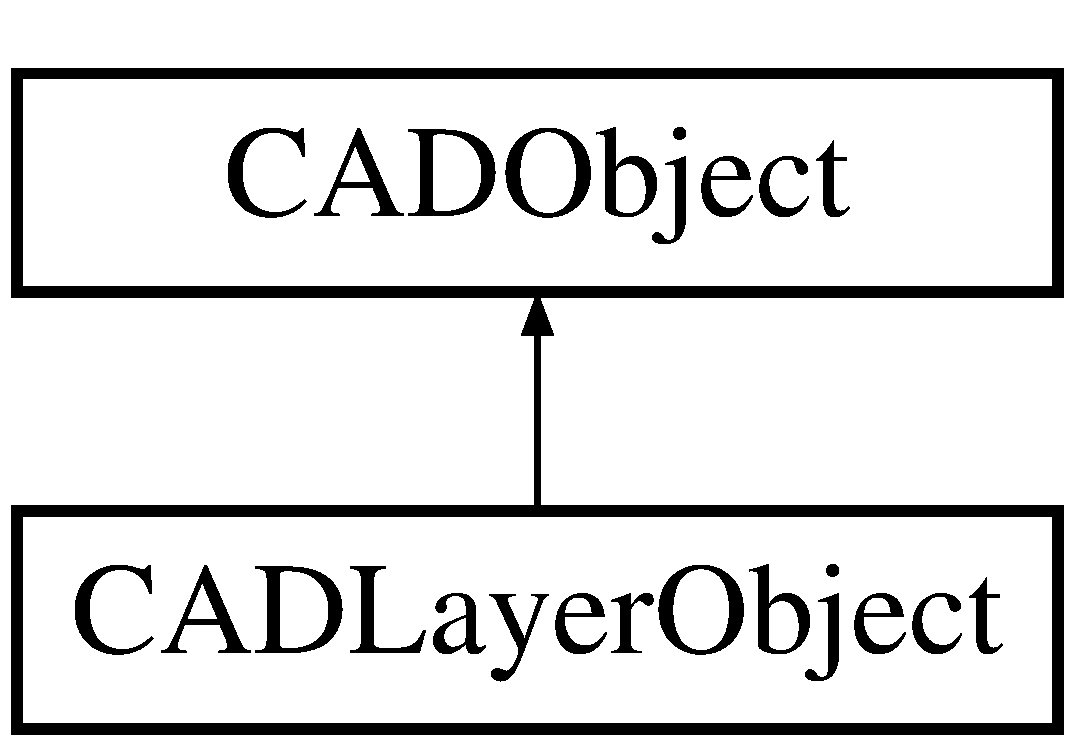
\includegraphics[height=2.000000cm]{class_c_a_d_layer_object}
\end{center}
\end{figure}
\subsection*{Public Attributes}
\begin{DoxyCompactItemize}
\item 
long {\bfseries n\+Object\+Size\+In\+Bits}\hypertarget{class_c_a_d_layer_object_a346f05db8a007fcbe6721d5a174f50bb}{}\label{class_c_a_d_layer_object_a346f05db8a007fcbe6721d5a174f50bb}

\item 
\hyperlink{class_c_a_d_handle}{C\+A\+D\+Handle} {\bfseries h\+Object\+Handle}\hypertarget{class_c_a_d_layer_object_aae4c1893aea45655c9c9c9d9112fc468}{}\label{class_c_a_d_layer_object_aae4c1893aea45655c9c9c9d9112fc468}

\item 
C\+A\+D\+Eed\+Array {\bfseries a\+E\+ED}\hypertarget{class_c_a_d_layer_object_a76e2fd562c00d5459ac572ccc1edb151}{}\label{class_c_a_d_layer_object_a76e2fd562c00d5459ac572ccc1edb151}

\item 
long {\bfseries n\+Num\+Reactors}\hypertarget{class_c_a_d_layer_object_ac99b41b7d5e72469d211a48bb16b3317}{}\label{class_c_a_d_layer_object_ac99b41b7d5e72469d211a48bb16b3317}

\item 
bool {\bfseries b\+No\+X\+Dictionary\+Present}\hypertarget{class_c_a_d_layer_object_a35da6d7c45d57986acd3d9e9a1afaf96}{}\label{class_c_a_d_layer_object_a35da6d7c45d57986acd3d9e9a1afaf96}

\item 
string {\bfseries s\+Layer\+Name}\hypertarget{class_c_a_d_layer_object_a0bf7815559565daa1c46b4cd0cbb5287}{}\label{class_c_a_d_layer_object_a0bf7815559565daa1c46b4cd0cbb5287}

\item 
bool {\bfseries b64\+Flag}\hypertarget{class_c_a_d_layer_object_afc343ad89ace97ee86119c03e7865e6e}{}\label{class_c_a_d_layer_object_afc343ad89ace97ee86119c03e7865e6e}

\item 
short {\bfseries d\+X\+Ref\+Index}\hypertarget{class_c_a_d_layer_object_a8b72d4df4dcff1ca436f386a25dae1c1}{}\label{class_c_a_d_layer_object_a8b72d4df4dcff1ca436f386a25dae1c1}

\item 
bool {\bfseries b\+X\+Dep}\hypertarget{class_c_a_d_layer_object_a08bafe1872d65a584564b03bce0d48e0}{}\label{class_c_a_d_layer_object_a08bafe1872d65a584564b03bce0d48e0}

\item 
bool {\bfseries b\+Frozen}\hypertarget{class_c_a_d_layer_object_abca68359b2ccf88f97adfb667608523d}{}\label{class_c_a_d_layer_object_abca68359b2ccf88f97adfb667608523d}

\item 
bool {\bfseries b\+On}\hypertarget{class_c_a_d_layer_object_ac77a183f0524bac046470d07b0dd9b83}{}\label{class_c_a_d_layer_object_ac77a183f0524bac046470d07b0dd9b83}

\item 
bool {\bfseries b\+Frozen\+In\+New\+V\+P\+O\+RT}\hypertarget{class_c_a_d_layer_object_ae0e03bd1ce72250592cb61db913c248d}{}\label{class_c_a_d_layer_object_ae0e03bd1ce72250592cb61db913c248d}

\item 
bool {\bfseries b\+Locked}\hypertarget{class_c_a_d_layer_object_a0f2fc2474750f6a9e0aff7dea81bbb4b}{}\label{class_c_a_d_layer_object_a0f2fc2474750f6a9e0aff7dea81bbb4b}

\item 
bool {\bfseries b\+Plotting\+Flag}\hypertarget{class_c_a_d_layer_object_a901c5594b4a9285552aae5c67db8f1ea}{}\label{class_c_a_d_layer_object_a901c5594b4a9285552aae5c67db8f1ea}

\item 
short {\bfseries d\+Line\+Weight}\hypertarget{class_c_a_d_layer_object_a77e1b8e4f87d24baf69a2431e9e7344a}{}\label{class_c_a_d_layer_object_a77e1b8e4f87d24baf69a2431e9e7344a}

\item 
short {\bfseries d\+C\+M\+Color}\hypertarget{class_c_a_d_layer_object_aaf50b4632db782b443c143fecf1aac78}{}\label{class_c_a_d_layer_object_aaf50b4632db782b443c143fecf1aac78}

\item 
\hyperlink{class_c_a_d_handle}{C\+A\+D\+Handle} {\bfseries h\+Layer\+Control}\hypertarget{class_c_a_d_layer_object_a1ab6f489c1fadac6256b0c53aa25624b}{}\label{class_c_a_d_layer_object_a1ab6f489c1fadac6256b0c53aa25624b}

\item 
C\+A\+D\+Handle\+Array {\bfseries h\+Reactors}\hypertarget{class_c_a_d_layer_object_a2e853537db4c848b1d34f599e352c089}{}\label{class_c_a_d_layer_object_a2e853537db4c848b1d34f599e352c089}

\item 
\hyperlink{class_c_a_d_handle}{C\+A\+D\+Handle} {\bfseries h\+X\+Dictionary}\hypertarget{class_c_a_d_layer_object_a252b8b120a49dabf0058e95a59b45409}{}\label{class_c_a_d_layer_object_a252b8b120a49dabf0058e95a59b45409}

\item 
\hyperlink{class_c_a_d_handle}{C\+A\+D\+Handle} {\bfseries h\+External\+Ref\+Block\+Handle}\hypertarget{class_c_a_d_layer_object_a45430119588e427c2059285140cd02d1}{}\label{class_c_a_d_layer_object_a45430119588e427c2059285140cd02d1}

\item 
\hyperlink{class_c_a_d_handle}{C\+A\+D\+Handle} {\bfseries h\+Plot\+Style}\hypertarget{class_c_a_d_layer_object_a0a53f93c4c3d7d6fa37230952ecc1bf3}{}\label{class_c_a_d_layer_object_a0a53f93c4c3d7d6fa37230952ecc1bf3}

\item 
\hyperlink{class_c_a_d_handle}{C\+A\+D\+Handle} {\bfseries h\+Material}\hypertarget{class_c_a_d_layer_object_aaaf5ecac578cde6bd7a02803581c6e4c}{}\label{class_c_a_d_layer_object_aaaf5ecac578cde6bd7a02803581c6e4c}

\item 
\hyperlink{class_c_a_d_handle}{C\+A\+D\+Handle} {\bfseries h\+L\+Type}\hypertarget{class_c_a_d_layer_object_a56401617297dedef2c828868ea5439c2}{}\label{class_c_a_d_layer_object_a56401617297dedef2c828868ea5439c2}

\item 
\hyperlink{class_c_a_d_handle}{C\+A\+D\+Handle} {\bfseries h\+Unknown\+Handle}\hypertarget{class_c_a_d_layer_object_abeba86f65459f22c4496a7aa48fee2a4}{}\label{class_c_a_d_layer_object_abeba86f65459f22c4496a7aa48fee2a4}

\end{DoxyCompactItemize}
\subsection*{Additional Inherited Members}


\subsection{Detailed Description}
The \hyperlink{class_c_a_d_layer_object}{C\+A\+D\+Layer\+Object} class. 

The documentation for this class was generated from the following files\+:\begin{DoxyCompactItemize}
\item 
cadobjects.\+h\item 
cadobjects.\+cpp\end{DoxyCompactItemize}

\hypertarget{class_c_a_d_line}{}\section{C\+A\+D\+Line Class Reference}
\label{class_c_a_d_line}\index{C\+A\+D\+Line@{C\+A\+D\+Line}}


Geometry class which represents a simple Line.  




{\ttfamily \#include $<$cadgeometry.\+h$>$}

Inheritance diagram for C\+A\+D\+Line\+:\begin{figure}[H]
\begin{center}
\leavevmode
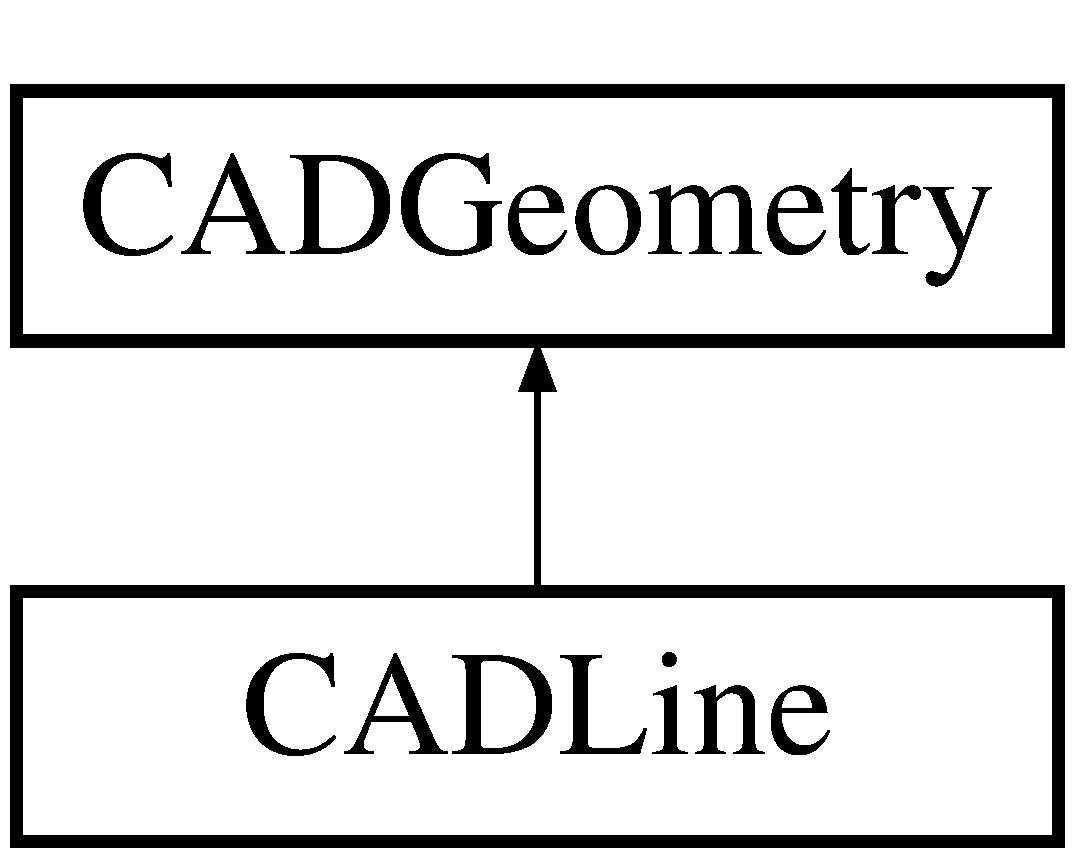
\includegraphics[height=2.000000cm]{class_c_a_d_line}
\end{center}
\end{figure}
\subsection*{Public Member Functions}
\begin{DoxyCompactItemize}
\item 
{\bfseries C\+A\+D\+Line} (const \hyperlink{class_c_a_d_point3_d}{C\+A\+D\+Point3D} \&start\+In, const \hyperlink{class_c_a_d_point3_d}{C\+A\+D\+Point3D} \&end\+In)\hypertarget{class_c_a_d_line_ac1b7a77ef2d8e853b6356554ddc0dcdc}{}\label{class_c_a_d_line_ac1b7a77ef2d8e853b6356554ddc0dcdc}

\item 
\hyperlink{class_c_a_d_point3_d}{C\+A\+D\+Point3D} {\bfseries get\+Start} () const \hypertarget{class_c_a_d_line_a721e80cf9219fb7acf24e33aa612218a}{}\label{class_c_a_d_line_a721e80cf9219fb7acf24e33aa612218a}

\item 
void {\bfseries set\+Start} (const \hyperlink{class_c_a_d_point3_d}{C\+A\+D\+Point3D} \&value)\hypertarget{class_c_a_d_line_a2ba1be49ca6cb424f4061feb72c7c63b}{}\label{class_c_a_d_line_a2ba1be49ca6cb424f4061feb72c7c63b}

\item 
\hyperlink{class_c_a_d_point3_d}{C\+A\+D\+Point3D} {\bfseries get\+End} () const \hypertarget{class_c_a_d_line_a0be6b3753da26f84a0c6f054ae3ce464}{}\label{class_c_a_d_line_a0be6b3753da26f84a0c6f054ae3ce464}

\item 
void {\bfseries set\+End} (const \hyperlink{class_c_a_d_point3_d}{C\+A\+D\+Point3D} \&value)\hypertarget{class_c_a_d_line_afe32345b45ce869e514ce6c03ed08f54}{}\label{class_c_a_d_line_afe32345b45ce869e514ce6c03ed08f54}

\item 
virtual void {\bfseries print} () const  override\hypertarget{class_c_a_d_line_ab5a0b4d286c07df3332e6926508774ff}{}\label{class_c_a_d_line_ab5a0b4d286c07df3332e6926508774ff}

\end{DoxyCompactItemize}
\subsection*{Protected Attributes}
\begin{DoxyCompactItemize}
\item 
\hyperlink{class_c_a_d_point3_d}{C\+A\+D\+Point3D} {\bfseries start}\hypertarget{class_c_a_d_line_a134324386aac13ead8439ca11c17b42b}{}\label{class_c_a_d_line_a134324386aac13ead8439ca11c17b42b}

\item 
\hyperlink{class_c_a_d_point3_d}{C\+A\+D\+Point3D} {\bfseries end}\hypertarget{class_c_a_d_line_a25a9d4f9a601ab16b83cb5f21d8c0f66}{}\label{class_c_a_d_line_a25a9d4f9a601ab16b83cb5f21d8c0f66}

\end{DoxyCompactItemize}
\subsection*{Additional Inherited Members}


\subsection{Detailed Description}
Geometry class which represents a simple Line. 

The documentation for this class was generated from the following files\+:\begin{DoxyCompactItemize}
\item 
cadgeometry.\+h\item 
cadgeometry.\+cpp\end{DoxyCompactItemize}

\hypertarget{class_c_a_d_line_object}{}\section{C\+A\+D\+Line\+Object Class Reference}
\label{class_c_a_d_line_object}\index{C\+A\+D\+Line\+Object@{C\+A\+D\+Line\+Object}}


The \hyperlink{class_c_a_d_line_object}{C\+A\+D\+Line\+Object} class.  




{\ttfamily \#include $<$cadobjects.\+h$>$}

Inheritance diagram for C\+A\+D\+Line\+Object\+:\begin{figure}[H]
\begin{center}
\leavevmode
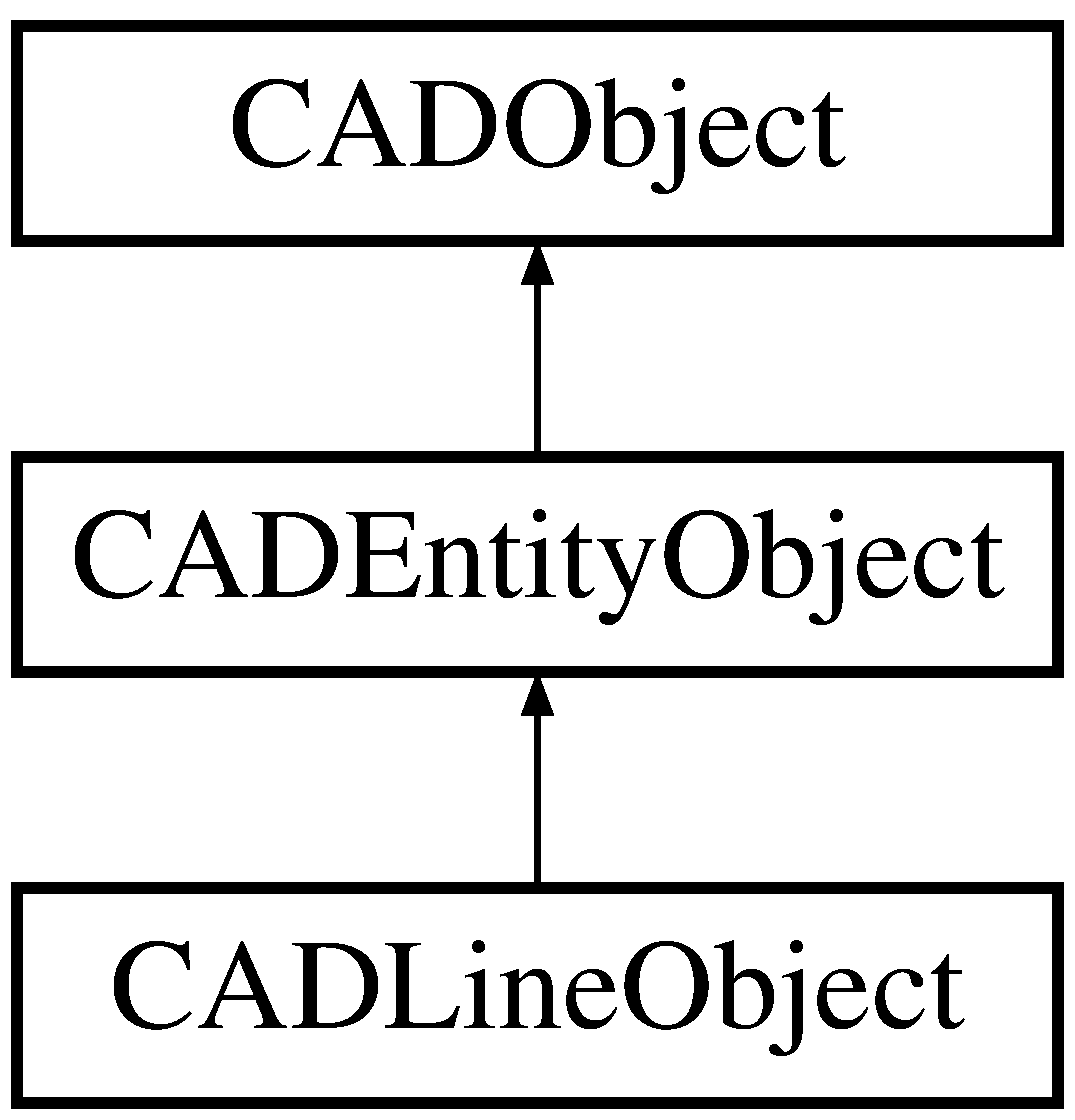
\includegraphics[height=3.000000cm]{class_c_a_d_line_object}
\end{center}
\end{figure}
\subsection*{Public Attributes}
\begin{DoxyCompactItemize}
\item 
\hyperlink{class_c_a_d_vector}{C\+A\+D\+Vector} {\bfseries vert\+Start}\hypertarget{class_c_a_d_line_object_af1f180bebce94d1bfc90b9c0a055d0d8}{}\label{class_c_a_d_line_object_af1f180bebce94d1bfc90b9c0a055d0d8}

\item 
\hyperlink{class_c_a_d_vector}{C\+A\+D\+Vector} {\bfseries vert\+End}\hypertarget{class_c_a_d_line_object_ab2322d276ee0e0979f711f9535207f19}{}\label{class_c_a_d_line_object_ab2322d276ee0e0979f711f9535207f19}

\item 
double {\bfseries df\+Thickness}\hypertarget{class_c_a_d_line_object_aca2ad5351f37fd17a3a1edbddce74c0d}{}\label{class_c_a_d_line_object_aca2ad5351f37fd17a3a1edbddce74c0d}

\item 
\hyperlink{class_c_a_d_vector}{C\+A\+D\+Vector} {\bfseries vect\+Extrusion}\hypertarget{class_c_a_d_line_object_a738374670fd5efb2fea017146aece25b}{}\label{class_c_a_d_line_object_a738374670fd5efb2fea017146aece25b}

\end{DoxyCompactItemize}
\subsection*{Additional Inherited Members}


\subsection{Detailed Description}
The \hyperlink{class_c_a_d_line_object}{C\+A\+D\+Line\+Object} class. 

The documentation for this class was generated from the following files\+:\begin{DoxyCompactItemize}
\item 
cadobjects.\+h\item 
cadobjects.\+cpp\end{DoxyCompactItemize}

\hypertarget{class_c_a_d_line_type_control_object}{}\section{C\+A\+D\+Line\+Type\+Control\+Object Class Reference}
\label{class_c_a_d_line_type_control_object}\index{C\+A\+D\+Line\+Type\+Control\+Object@{C\+A\+D\+Line\+Type\+Control\+Object}}


The \hyperlink{class_c_a_d_line_type_control_object}{C\+A\+D\+Line\+Type\+Control\+Object} class.  




{\ttfamily \#include $<$cadobjects.\+h$>$}

Inheritance diagram for C\+A\+D\+Line\+Type\+Control\+Object\+:\begin{figure}[H]
\begin{center}
\leavevmode
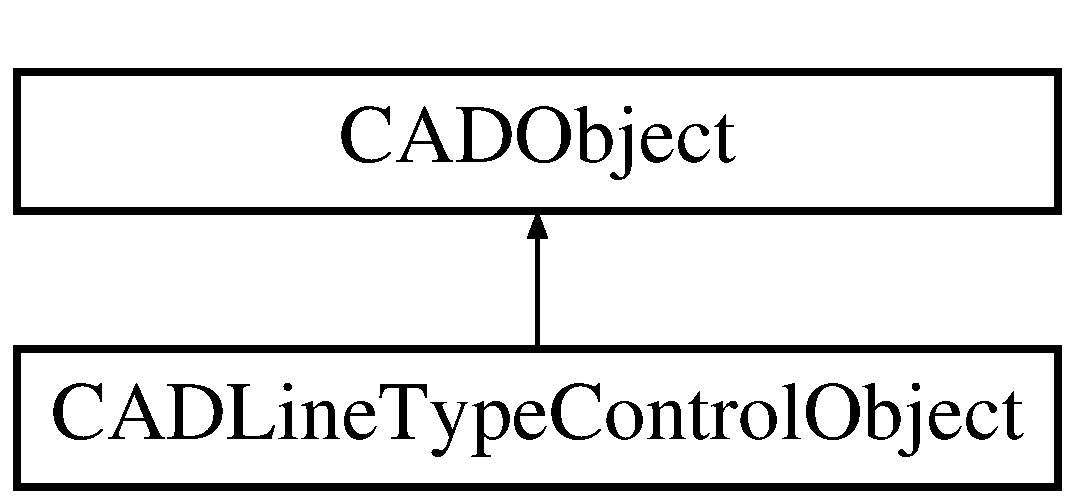
\includegraphics[height=2.000000cm]{class_c_a_d_line_type_control_object}
\end{center}
\end{figure}
\subsection*{Public Attributes}
\begin{DoxyCompactItemize}
\item 
long {\bfseries n\+Object\+Size\+In\+Bits}\hypertarget{class_c_a_d_line_type_control_object_af3b8b4fe129e604d4a24e689c98b3ee6}{}\label{class_c_a_d_line_type_control_object_af3b8b4fe129e604d4a24e689c98b3ee6}

\item 
\hyperlink{class_c_a_d_handle}{C\+A\+D\+Handle} {\bfseries h\+Object\+Handle}\hypertarget{class_c_a_d_line_type_control_object_a8e2eacc98ca932e07a050d1364d579b7}{}\label{class_c_a_d_line_type_control_object_a8e2eacc98ca932e07a050d1364d579b7}

\item 
C\+A\+D\+Eed\+Array {\bfseries a\+E\+ED}\hypertarget{class_c_a_d_line_type_control_object_a1f99a732cdb509bc6d044b4e0cd2a3b5}{}\label{class_c_a_d_line_type_control_object_a1f99a732cdb509bc6d044b4e0cd2a3b5}

\item 
long {\bfseries n\+Num\+Reactors}\hypertarget{class_c_a_d_line_type_control_object_a534dc4644f6cfb7845d338a3c1adebdb}{}\label{class_c_a_d_line_type_control_object_a534dc4644f6cfb7845d338a3c1adebdb}

\item 
bool {\bfseries b\+No\+X\+Dictionary\+Present}\hypertarget{class_c_a_d_line_type_control_object_afd13099422c4bcf4e49774636e6dfcf9}{}\label{class_c_a_d_line_type_control_object_afd13099422c4bcf4e49774636e6dfcf9}

\item 
long {\bfseries n\+Num\+Entries}\hypertarget{class_c_a_d_line_type_control_object_ad970b8326cadff257be066bc8e8082f8}{}\label{class_c_a_d_line_type_control_object_ad970b8326cadff257be066bc8e8082f8}

\item 
\hyperlink{class_c_a_d_handle}{C\+A\+D\+Handle} {\bfseries h\+Null}\hypertarget{class_c_a_d_line_type_control_object_a296c4b1aaef96eb68b882f72b0eea876}{}\label{class_c_a_d_line_type_control_object_a296c4b1aaef96eb68b882f72b0eea876}

\item 
\hyperlink{class_c_a_d_handle}{C\+A\+D\+Handle} {\bfseries h\+X\+Dictionary}\hypertarget{class_c_a_d_line_type_control_object_a7e113a7c4f636cb25ec4e18388c4833d}{}\label{class_c_a_d_line_type_control_object_a7e113a7c4f636cb25ec4e18388c4833d}

\item 
C\+A\+D\+Handle\+Array {\bfseries h\+L\+Types}\hypertarget{class_c_a_d_line_type_control_object_a35b132f5150f9b1766cb2e2aa322e857}{}\label{class_c_a_d_line_type_control_object_a35b132f5150f9b1766cb2e2aa322e857}

\end{DoxyCompactItemize}
\subsection*{Additional Inherited Members}


\subsection{Detailed Description}
The \hyperlink{class_c_a_d_line_type_control_object}{C\+A\+D\+Line\+Type\+Control\+Object} class. 

The documentation for this class was generated from the following files\+:\begin{DoxyCompactItemize}
\item 
cadobjects.\+h\item 
cadobjects.\+cpp\end{DoxyCompactItemize}

\hypertarget{class_c_a_d_line_type_object}{}\section{C\+A\+D\+Line\+Type\+Object Class Reference}
\label{class_c_a_d_line_type_object}\index{C\+A\+D\+Line\+Type\+Object@{C\+A\+D\+Line\+Type\+Object}}


The \hyperlink{class_c_a_d_line_type_object}{C\+A\+D\+Line\+Type\+Object} class.  




{\ttfamily \#include $<$cadobjects.\+h$>$}

Inheritance diagram for C\+A\+D\+Line\+Type\+Object\+:\begin{figure}[H]
\begin{center}
\leavevmode
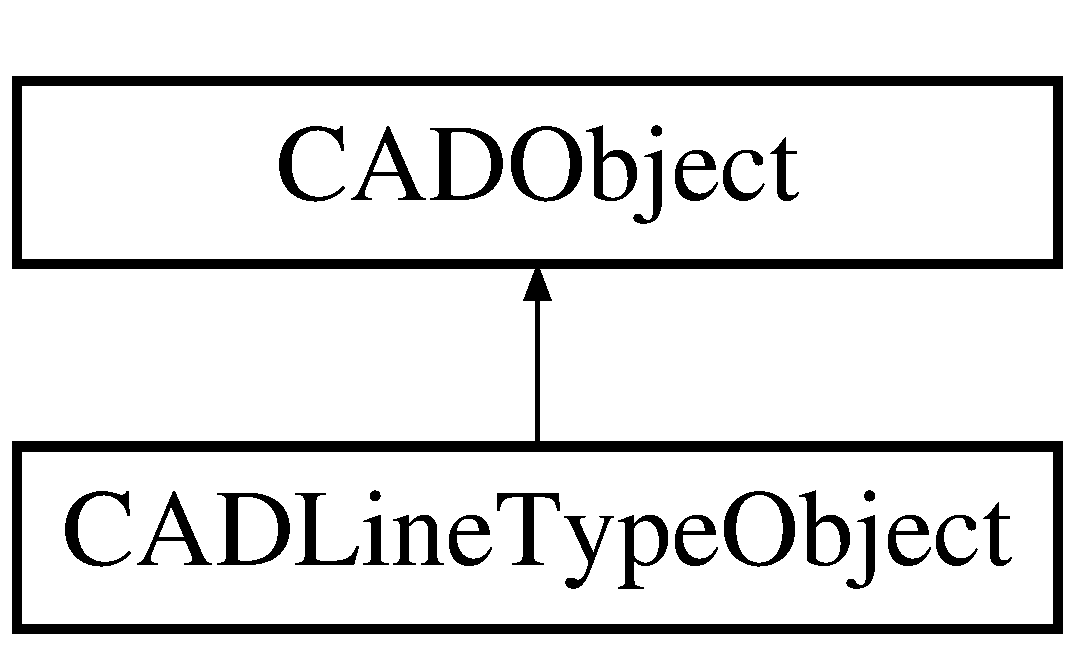
\includegraphics[height=2.000000cm]{class_c_a_d_line_type_object}
\end{center}
\end{figure}
\subsection*{Public Attributes}
\begin{DoxyCompactItemize}
\item 
long {\bfseries n\+Object\+Size\+In\+Bits}\hypertarget{class_c_a_d_line_type_object_a27b462aad1b628feb25b9a0810620d3a}{}\label{class_c_a_d_line_type_object_a27b462aad1b628feb25b9a0810620d3a}

\item 
\hyperlink{class_c_a_d_handle}{C\+A\+D\+Handle} {\bfseries h\+Object\+Handle}\hypertarget{class_c_a_d_line_type_object_a00d63bba5e2e02633c0650f78ff26d21}{}\label{class_c_a_d_line_type_object_a00d63bba5e2e02633c0650f78ff26d21}

\item 
C\+A\+D\+Eed\+Array {\bfseries a\+E\+ED}\hypertarget{class_c_a_d_line_type_object_a302f93d6c8444923ac1ca16b903c0c44}{}\label{class_c_a_d_line_type_object_a302f93d6c8444923ac1ca16b903c0c44}

\item 
long {\bfseries n\+Num\+Reactors}\hypertarget{class_c_a_d_line_type_object_a10bab052d88fe9e32127059da93fa711}{}\label{class_c_a_d_line_type_object_a10bab052d88fe9e32127059da93fa711}

\item 
bool {\bfseries b\+No\+X\+Dictionary\+Present}\hypertarget{class_c_a_d_line_type_object_a0b28c8e1029d8dd953738ea670e19439}{}\label{class_c_a_d_line_type_object_a0b28c8e1029d8dd953738ea670e19439}

\item 
string {\bfseries s\+Entry\+Name}\hypertarget{class_c_a_d_line_type_object_a7d0cdfde87b851fb761eec1b0b6e16c7}{}\label{class_c_a_d_line_type_object_a7d0cdfde87b851fb761eec1b0b6e16c7}

\item 
bool {\bfseries b64\+Flag}\hypertarget{class_c_a_d_line_type_object_afaeb8ff7d051316332e1a7ad4205a482}{}\label{class_c_a_d_line_type_object_afaeb8ff7d051316332e1a7ad4205a482}

\item 
short {\bfseries d\+X\+Ref\+Index}\hypertarget{class_c_a_d_line_type_object_abc555dfe7bf5a3b065f96e207842551b}{}\label{class_c_a_d_line_type_object_abc555dfe7bf5a3b065f96e207842551b}

\item 
bool {\bfseries b\+X\+Dep}\hypertarget{class_c_a_d_line_type_object_a3a515da2e85d53c7e7110869e98810ce}{}\label{class_c_a_d_line_type_object_a3a515da2e85d53c7e7110869e98810ce}

\item 
string {\bfseries s\+Description}\hypertarget{class_c_a_d_line_type_object_a68ac789a255fd8d31b0406f98e2b2d43}{}\label{class_c_a_d_line_type_object_a68ac789a255fd8d31b0406f98e2b2d43}

\item 
double {\bfseries df\+Pattern\+Len}\hypertarget{class_c_a_d_line_type_object_ab9dea99ba41b09d22ae274df9017207e}{}\label{class_c_a_d_line_type_object_ab9dea99ba41b09d22ae274df9017207e}

\item 
unsigned char {\bfseries d\+Alignment}\hypertarget{class_c_a_d_line_type_object_aa7d07e109579ec14777bc2925f7a7a83}{}\label{class_c_a_d_line_type_object_aa7d07e109579ec14777bc2925f7a7a83}

\item 
unsigned char {\bfseries n\+Num\+Dashes}\hypertarget{class_c_a_d_line_type_object_acc3f0317f1efb3a966e69c65d347bad0}{}\label{class_c_a_d_line_type_object_acc3f0317f1efb3a966e69c65d347bad0}

\item 
vector$<$ \hyperlink{struct__dash}{C\+A\+D\+Dash} $>$ {\bfseries ast\+Dashes}\hypertarget{class_c_a_d_line_type_object_a5bb61e722df2910d7fb9b08348ff9b69}{}\label{class_c_a_d_line_type_object_a5bb61e722df2910d7fb9b08348ff9b69}

\item 
vector$<$ unsigned char $>$ {\bfseries aby\+Text\+Area}\hypertarget{class_c_a_d_line_type_object_a2741c1668d0127266ddde995229f4435}{}\label{class_c_a_d_line_type_object_a2741c1668d0127266ddde995229f4435}

\item 
\hyperlink{class_c_a_d_handle}{C\+A\+D\+Handle} {\bfseries h\+L\+T\+Control}\hypertarget{class_c_a_d_line_type_object_a88b2119b0ffa7035dde85fe291c78a36}{}\label{class_c_a_d_line_type_object_a88b2119b0ffa7035dde85fe291c78a36}

\item 
C\+A\+D\+Handle\+Array {\bfseries h\+Reactors}\hypertarget{class_c_a_d_line_type_object_aa530511bedc86c7ba1abc3fc5772c75d}{}\label{class_c_a_d_line_type_object_aa530511bedc86c7ba1abc3fc5772c75d}

\item 
\hyperlink{class_c_a_d_handle}{C\+A\+D\+Handle} {\bfseries h\+X\+Dictionary}\hypertarget{class_c_a_d_line_type_object_a7090a83d655ad546f1da0616e89680be}{}\label{class_c_a_d_line_type_object_a7090a83d655ad546f1da0616e89680be}

\item 
\hyperlink{class_c_a_d_handle}{C\+A\+D\+Handle} {\bfseries h\+X\+Ref\+Block}\hypertarget{class_c_a_d_line_type_object_a478c1b4b4f7d674aa4048d90394f8ce5}{}\label{class_c_a_d_line_type_object_a478c1b4b4f7d674aa4048d90394f8ce5}

\item 
C\+A\+D\+Handle\+Array {\bfseries h\+Shapefiles}\hypertarget{class_c_a_d_line_type_object_abfc8de123895688bb4765a867b165864}{}\label{class_c_a_d_line_type_object_abfc8de123895688bb4765a867b165864}

\end{DoxyCompactItemize}
\subsection*{Additional Inherited Members}


\subsection{Detailed Description}
The \hyperlink{class_c_a_d_line_type_object}{C\+A\+D\+Line\+Type\+Object} class. 

The documentation for this class was generated from the following files\+:\begin{DoxyCompactItemize}
\item 
cadobjects.\+h\item 
cadobjects.\+cpp\end{DoxyCompactItemize}

\hypertarget{class_c_a_d_l_w_polyline}{}\section{C\+A\+D\+L\+W\+Polyline Class Reference}
\label{class_c_a_d_l_w_polyline}\index{C\+A\+D\+L\+W\+Polyline@{C\+A\+D\+L\+W\+Polyline}}


Geometry class which represents L\+W\+Polyline.  




{\ttfamily \#include $<$cadgeometry.\+h$>$}

Inheritance diagram for C\+A\+D\+L\+W\+Polyline\+:\begin{figure}[H]
\begin{center}
\leavevmode
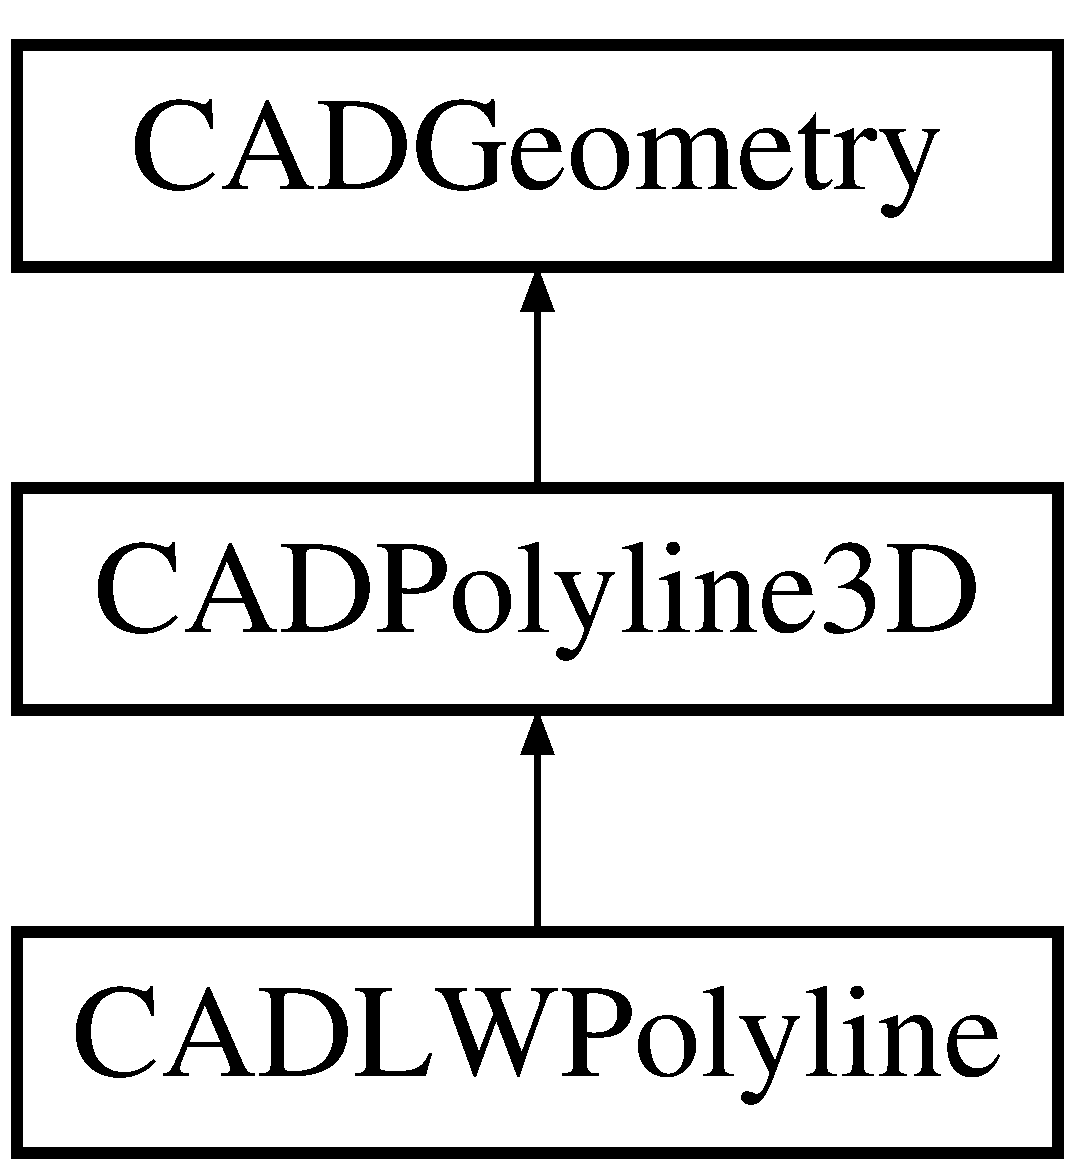
\includegraphics[height=3.000000cm]{class_c_a_d_l_w_polyline}
\end{center}
\end{figure}
\subsection*{Public Member Functions}
\begin{DoxyCompactItemize}
\item 
virtual void {\bfseries print} () const  override\hypertarget{class_c_a_d_l_w_polyline_a2c0a073ab6f626fbef987d3ac5c98b19}{}\label{class_c_a_d_l_w_polyline_a2c0a073ab6f626fbef987d3ac5c98b19}

\item 
double {\bfseries get\+Const\+Width} () const \hypertarget{class_c_a_d_l_w_polyline_a0ee3571f18e5c2a3f755ab7ef7b979e3}{}\label{class_c_a_d_l_w_polyline_a0ee3571f18e5c2a3f755ab7ef7b979e3}

\item 
void {\bfseries set\+Const\+Width} (double value)\hypertarget{class_c_a_d_l_w_polyline_a59e3ac8ba0ca76eef5a44e96e9937f1e}{}\label{class_c_a_d_l_w_polyline_a59e3ac8ba0ca76eef5a44e96e9937f1e}

\item 
double {\bfseries get\+Elevation} () const \hypertarget{class_c_a_d_l_w_polyline_a48dd80c3b22fd15365503f717932d426}{}\label{class_c_a_d_l_w_polyline_a48dd80c3b22fd15365503f717932d426}

\item 
void {\bfseries set\+Elevation} (double value)\hypertarget{class_c_a_d_l_w_polyline_af6ce34bb296f07f9ea1988aff184f86d}{}\label{class_c_a_d_l_w_polyline_af6ce34bb296f07f9ea1988aff184f86d}

\item 
\hyperlink{class_c_a_d_vector}{C\+A\+D\+Vector} {\bfseries get\+Vect\+Extrusion} () const \hypertarget{class_c_a_d_l_w_polyline_ab73d4a3b556ee073c3f94496a052f378}{}\label{class_c_a_d_l_w_polyline_ab73d4a3b556ee073c3f94496a052f378}

\item 
void {\bfseries set\+Vect\+Extrusion} (const \hyperlink{class_c_a_d_vector}{C\+A\+D\+Vector} \&value)\hypertarget{class_c_a_d_l_w_polyline_a7e06f07ab12407aa862c7f000cb1b827}{}\label{class_c_a_d_l_w_polyline_a7e06f07ab12407aa862c7f000cb1b827}

\item 
vector$<$ pair$<$ double, double $>$ $>$ {\bfseries get\+Widths} () const \hypertarget{class_c_a_d_l_w_polyline_ab4b812740b0338054a9176fd79ca822c}{}\label{class_c_a_d_l_w_polyline_ab4b812740b0338054a9176fd79ca822c}

\item 
void {\bfseries set\+Widths} (const vector$<$ pair$<$ double, double $>$ $>$ \&value)\hypertarget{class_c_a_d_l_w_polyline_ae8580bdd80ad48caf2ccafce9c230cba}{}\label{class_c_a_d_l_w_polyline_ae8580bdd80ad48caf2ccafce9c230cba}

\end{DoxyCompactItemize}
\subsection*{Protected Attributes}
\begin{DoxyCompactItemize}
\item 
double {\bfseries const\+Width}\hypertarget{class_c_a_d_l_w_polyline_aa0e89d7b67e44eff0a8168cd0410d09c}{}\label{class_c_a_d_l_w_polyline_aa0e89d7b67e44eff0a8168cd0410d09c}

\item 
double {\bfseries elevation}\hypertarget{class_c_a_d_l_w_polyline_a23e9200c2b4015eb1616526e02577bee}{}\label{class_c_a_d_l_w_polyline_a23e9200c2b4015eb1616526e02577bee}

\item 
\hyperlink{class_c_a_d_vector}{C\+A\+D\+Vector} {\bfseries vect\+Extrusion}\hypertarget{class_c_a_d_l_w_polyline_a9e02be37368c57e9d0624590af5b054d}{}\label{class_c_a_d_l_w_polyline_a9e02be37368c57e9d0624590af5b054d}

\item 
vector$<$ pair$<$ double, double $>$ $>$ {\bfseries widths}\hypertarget{class_c_a_d_l_w_polyline_a264af25fecf4a94f0c1fe65f368217ce}{}\label{class_c_a_d_l_w_polyline_a264af25fecf4a94f0c1fe65f368217ce}

\end{DoxyCompactItemize}
\subsection*{Additional Inherited Members}


\subsection{Detailed Description}
Geometry class which represents L\+W\+Polyline. 

The documentation for this class was generated from the following files\+:\begin{DoxyCompactItemize}
\item 
cadgeometry.\+h\item 
cadgeometry.\+cpp\end{DoxyCompactItemize}

\hypertarget{class_c_a_d_l_w_polyline_object}{}\section{C\+A\+D\+L\+W\+Polyline\+Object Class Reference}
\label{class_c_a_d_l_w_polyline_object}\index{C\+A\+D\+L\+W\+Polyline\+Object@{C\+A\+D\+L\+W\+Polyline\+Object}}


The \hyperlink{class_c_a_d_l_w_polyline_object}{C\+A\+D\+L\+W\+Polyline\+Object} class.  




{\ttfamily \#include $<$cadobjects.\+h$>$}

Inheritance diagram for C\+A\+D\+L\+W\+Polyline\+Object\+:\begin{figure}[H]
\begin{center}
\leavevmode
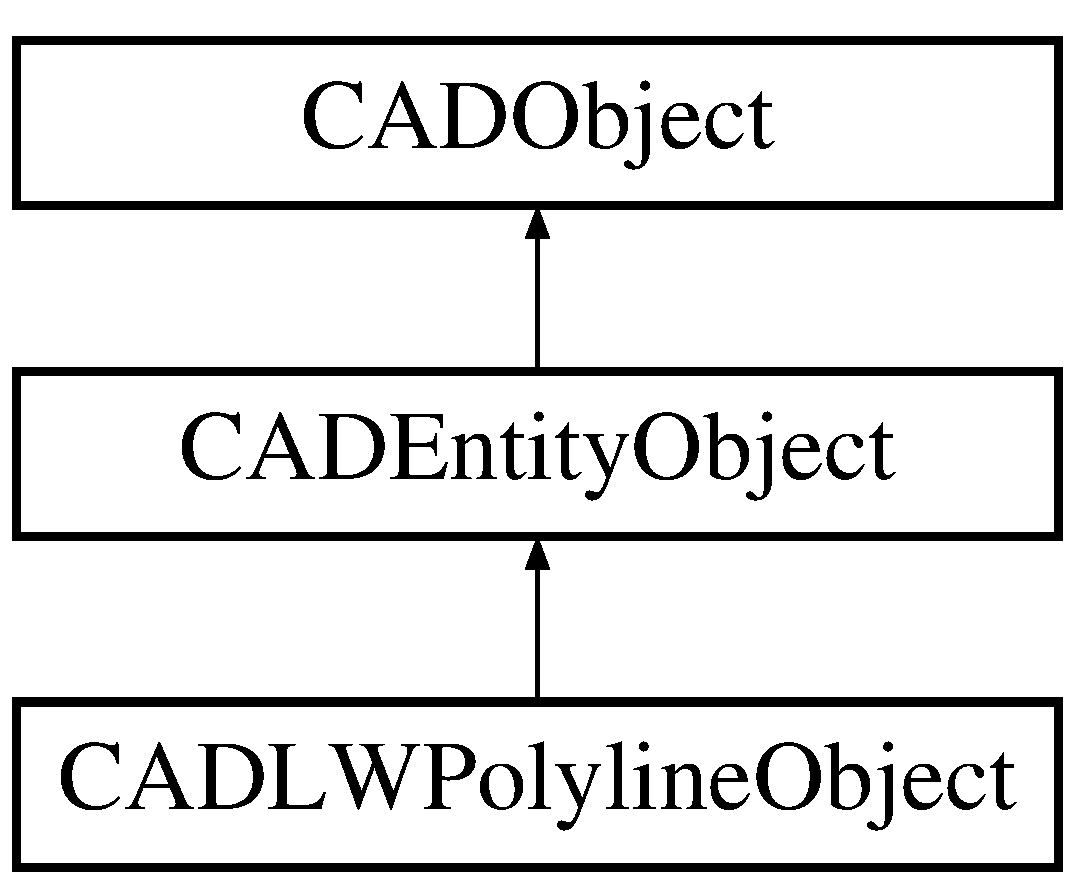
\includegraphics[height=3.000000cm]{class_c_a_d_l_w_polyline_object}
\end{center}
\end{figure}
\subsection*{Public Attributes}
\begin{DoxyCompactItemize}
\item 
double {\bfseries df\+Const\+Width}\hypertarget{class_c_a_d_l_w_polyline_object_a72ea94f5fb155eca94eb1a11ff8c3884}{}\label{class_c_a_d_l_w_polyline_object_a72ea94f5fb155eca94eb1a11ff8c3884}

\item 
double {\bfseries df\+Elevation}\hypertarget{class_c_a_d_l_w_polyline_object_a454ad8049c619d10a9b7ad6751e2ce98}{}\label{class_c_a_d_l_w_polyline_object_a454ad8049c619d10a9b7ad6751e2ce98}

\item 
double {\bfseries df\+Thickness}\hypertarget{class_c_a_d_l_w_polyline_object_a4bf7962c24f0d87dbd8b18d1625f1d49}{}\label{class_c_a_d_l_w_polyline_object_a4bf7962c24f0d87dbd8b18d1625f1d49}

\item 
\hyperlink{class_c_a_d_vector}{C\+A\+D\+Vector} {\bfseries vect\+Extrusion}\hypertarget{class_c_a_d_l_w_polyline_object_ad3eb54192045128229508655fbc13c5f}{}\label{class_c_a_d_l_w_polyline_object_ad3eb54192045128229508655fbc13c5f}

\item 
vector$<$ \hyperlink{class_c_a_d_vector}{C\+A\+D\+Vector} $>$ {\bfseries avert\+Vertexes}\hypertarget{class_c_a_d_l_w_polyline_object_a15372d1fb367f523a543a1924eddb01b}{}\label{class_c_a_d_l_w_polyline_object_a15372d1fb367f523a543a1924eddb01b}

\item 
vector$<$ double $>$ {\bfseries adf\+Bulges}\hypertarget{class_c_a_d_l_w_polyline_object_a64797a790804ef43a725d1dc22e7c347}{}\label{class_c_a_d_l_w_polyline_object_a64797a790804ef43a725d1dc22e7c347}

\item 
vector$<$ short $>$ {\bfseries ad\+Vertexes\+ID}\hypertarget{class_c_a_d_l_w_polyline_object_a1b880471d19186c74f8b7384de574aef}{}\label{class_c_a_d_l_w_polyline_object_a1b880471d19186c74f8b7384de574aef}

\item 
vector$<$ pair$<$ double, double $>$ $>$ {\bfseries ast\+Widths}\hypertarget{class_c_a_d_l_w_polyline_object_a0e1d0b7776c4fd058982148392cc100c}{}\label{class_c_a_d_l_w_polyline_object_a0e1d0b7776c4fd058982148392cc100c}

\end{DoxyCompactItemize}
\subsection*{Additional Inherited Members}


\subsection{Detailed Description}
The \hyperlink{class_c_a_d_l_w_polyline_object}{C\+A\+D\+L\+W\+Polyline\+Object} class. 

The documentation for this class was generated from the following files\+:\begin{DoxyCompactItemize}
\item 
cadobjects.\+h\item 
cadobjects.\+cpp\end{DoxyCompactItemize}

\hypertarget{class_c_a_d_m_insert_object}{}\section{C\+A\+D\+M\+Insert\+Object Class Reference}
\label{class_c_a_d_m_insert_object}\index{C\+A\+D\+M\+Insert\+Object@{C\+A\+D\+M\+Insert\+Object}}


The \hyperlink{class_c_a_d_m_insert_object}{C\+A\+D\+M\+Insert\+Object} class.  




{\ttfamily \#include $<$cadobjects.\+h$>$}

Inheritance diagram for C\+A\+D\+M\+Insert\+Object\+:\begin{figure}[H]
\begin{center}
\leavevmode
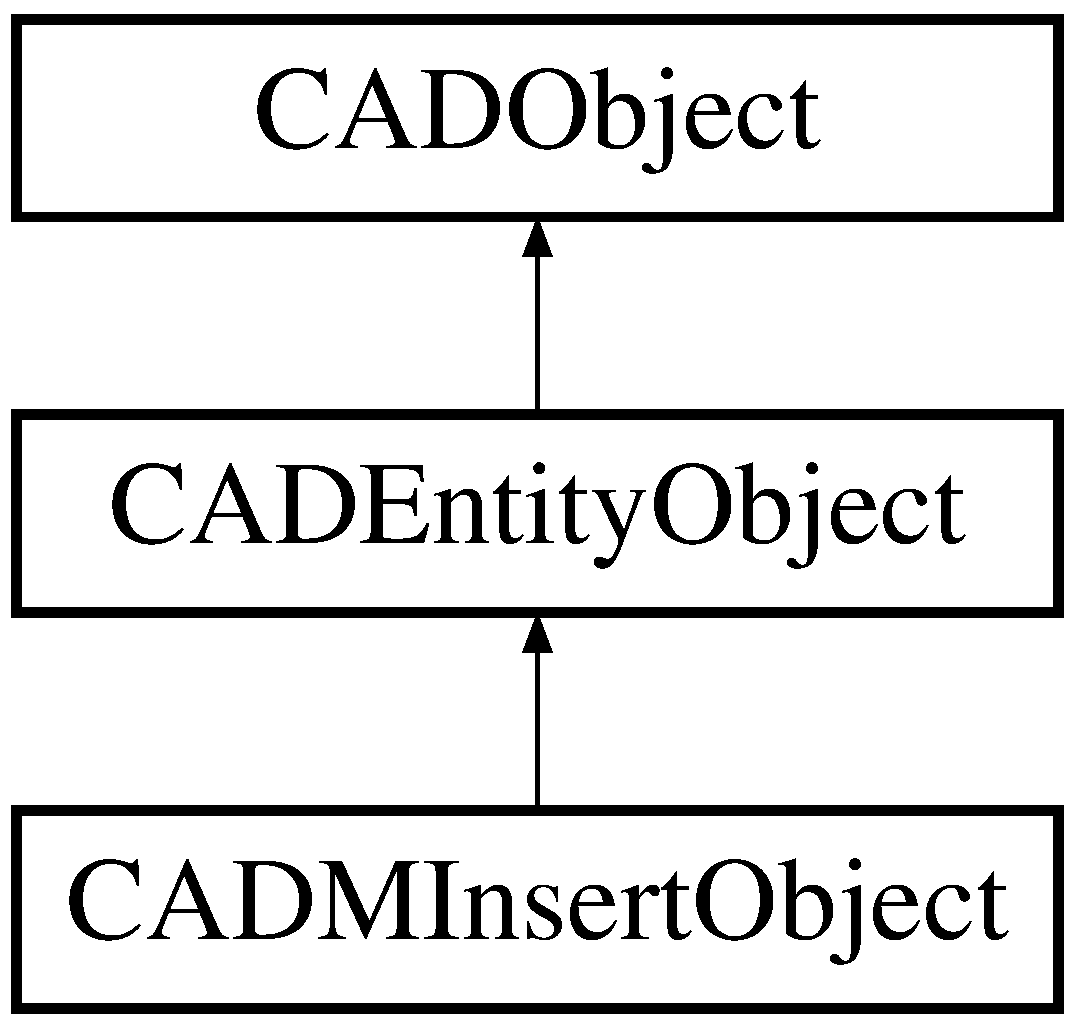
\includegraphics[height=3.000000cm]{class_c_a_d_m_insert_object}
\end{center}
\end{figure}
\subsection*{Public Attributes}
\begin{DoxyCompactItemize}
\item 
\hyperlink{class_c_a_d_vector}{C\+A\+D\+Vector} {\bfseries vert\+Insertion\+Point}\hypertarget{class_c_a_d_m_insert_object_add31138b5f343ac0627281809e3c1ebe}{}\label{class_c_a_d_m_insert_object_add31138b5f343ac0627281809e3c1ebe}

\item 
\hyperlink{class_c_a_d_vector}{C\+A\+D\+Vector} {\bfseries vert\+Scales}\hypertarget{class_c_a_d_m_insert_object_adbb9c4d6ff926c501f3ea08ea5ca182c}{}\label{class_c_a_d_m_insert_object_adbb9c4d6ff926c501f3ea08ea5ca182c}

\item 
double {\bfseries df\+Rotation}\hypertarget{class_c_a_d_m_insert_object_a7eee9537473e0545785c1768ab439ee0}{}\label{class_c_a_d_m_insert_object_a7eee9537473e0545785c1768ab439ee0}

\item 
\hyperlink{class_c_a_d_vector}{C\+A\+D\+Vector} {\bfseries vect\+Extrusion}\hypertarget{class_c_a_d_m_insert_object_af555c36d3d8ac969aa64429be0e84c4d}{}\label{class_c_a_d_m_insert_object_af555c36d3d8ac969aa64429be0e84c4d}

\item 
bool {\bfseries b\+Has\+Attribs}\hypertarget{class_c_a_d_m_insert_object_af54ef417d4e6bc4a14ef48033c786cdb}{}\label{class_c_a_d_m_insert_object_af54ef417d4e6bc4a14ef48033c786cdb}

\item 
long {\bfseries n\+Objects\+Owned}\hypertarget{class_c_a_d_m_insert_object_aa47ceb6de8892000f5d9df070bfc70b8}{}\label{class_c_a_d_m_insert_object_aa47ceb6de8892000f5d9df070bfc70b8}

\item 
short {\bfseries n\+Num\+Cols}\hypertarget{class_c_a_d_m_insert_object_a9857c4047e0caf7b40710651f24c4293}{}\label{class_c_a_d_m_insert_object_a9857c4047e0caf7b40710651f24c4293}

\item 
short {\bfseries n\+Num\+Rows}\hypertarget{class_c_a_d_m_insert_object_a4c569cedc997e2c3307fabe980f922c2}{}\label{class_c_a_d_m_insert_object_a4c569cedc997e2c3307fabe980f922c2}

\item 
short {\bfseries n\+Col\+Spacing}\hypertarget{class_c_a_d_m_insert_object_acb056fb8650c1f4c3e3a15f77ac174be}{}\label{class_c_a_d_m_insert_object_acb056fb8650c1f4c3e3a15f77ac174be}

\item 
short {\bfseries n\+Row\+Spacing}\hypertarget{class_c_a_d_m_insert_object_ab89dd6e7dcde3f3148e86aaf5bded2c5}{}\label{class_c_a_d_m_insert_object_ab89dd6e7dcde3f3148e86aaf5bded2c5}

\item 
\hyperlink{class_c_a_d_handle}{C\+A\+D\+Handle} {\bfseries h\+Block\+Header}\hypertarget{class_c_a_d_m_insert_object_a75ad8b3bf7a466a5a1050747627e808f}{}\label{class_c_a_d_m_insert_object_a75ad8b3bf7a466a5a1050747627e808f}

\item 
C\+A\+D\+Handle\+Array {\bfseries h\+Atrribs}\hypertarget{class_c_a_d_m_insert_object_ac77bf3fd0f32c983366577e823025053}{}\label{class_c_a_d_m_insert_object_ac77bf3fd0f32c983366577e823025053}

\item 
\hyperlink{class_c_a_d_handle}{C\+A\+D\+Handle} {\bfseries h\+Seqend}\hypertarget{class_c_a_d_m_insert_object_a1c7817910374d5ba23c22cafa9745cf7}{}\label{class_c_a_d_m_insert_object_a1c7817910374d5ba23c22cafa9745cf7}

\end{DoxyCompactItemize}
\subsection*{Additional Inherited Members}


\subsection{Detailed Description}
The \hyperlink{class_c_a_d_m_insert_object}{C\+A\+D\+M\+Insert\+Object} class. 

The documentation for this class was generated from the following files\+:\begin{DoxyCompactItemize}
\item 
cadobjects.\+h\item 
cadobjects.\+cpp\end{DoxyCompactItemize}

\hypertarget{class_c_a_d_m_line}{}\section{C\+A\+D\+M\+Line Class Reference}
\label{class_c_a_d_m_line}\index{C\+A\+D\+M\+Line@{C\+A\+D\+M\+Line}}


Geometry class which represents M\+Line.  




{\ttfamily \#include $<$cadgeometry.\+h$>$}

Inheritance diagram for C\+A\+D\+M\+Line\+:\begin{figure}[H]
\begin{center}
\leavevmode
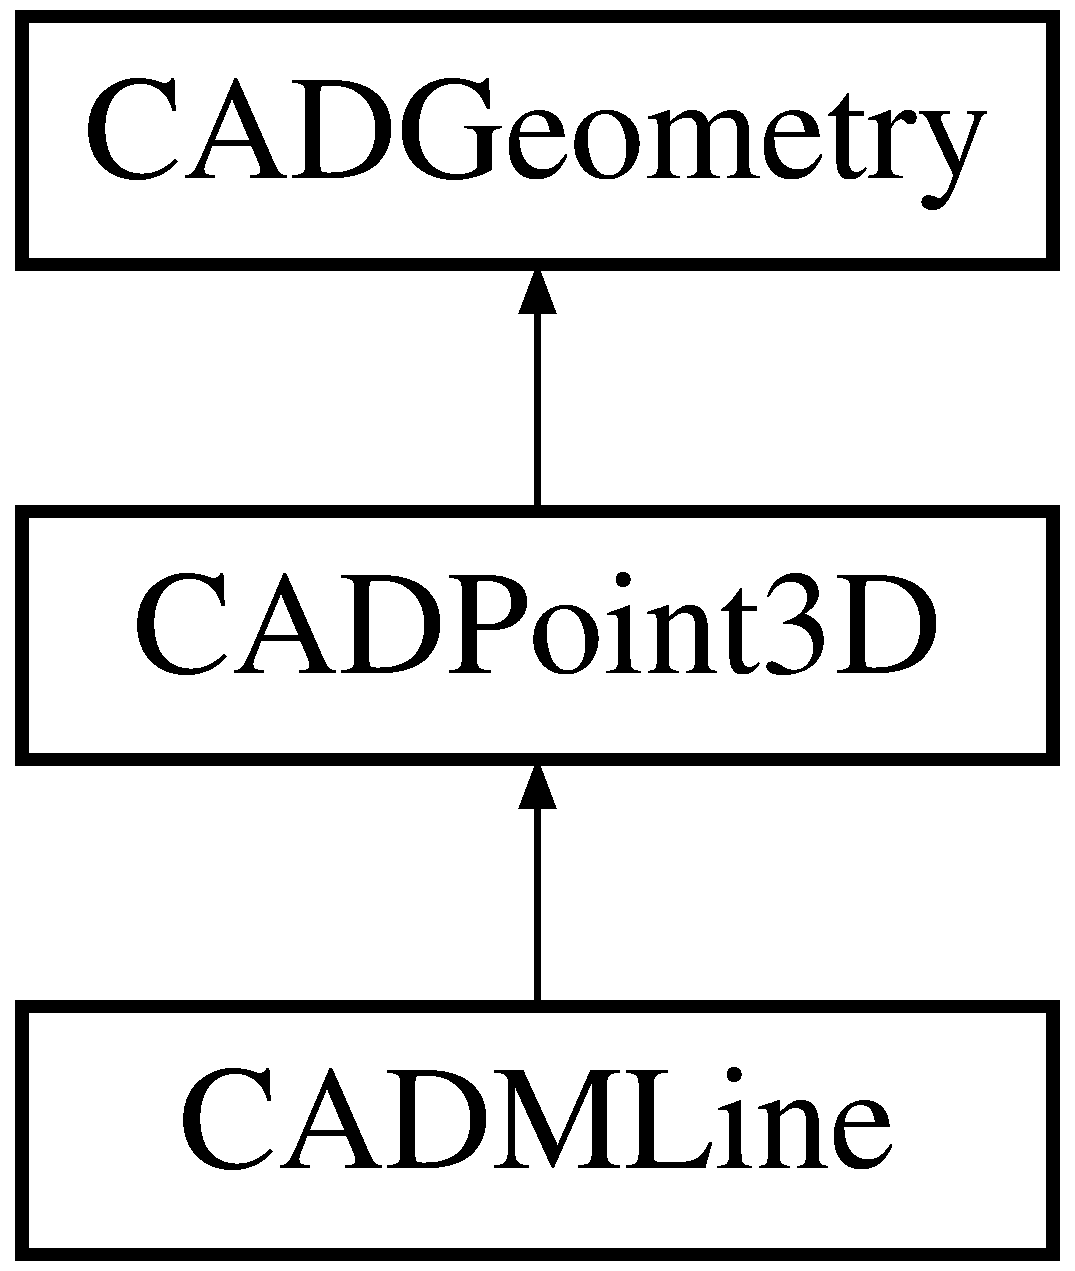
\includegraphics[height=3.000000cm]{class_c_a_d_m_line}
\end{center}
\end{figure}
\subsection*{Public Member Functions}
\begin{DoxyCompactItemize}
\item 
virtual void {\bfseries print} () const  override\hypertarget{class_c_a_d_m_line_a13ddedaa98d8c2053b2b12be667d3450}{}\label{class_c_a_d_m_line_a13ddedaa98d8c2053b2b12be667d3450}

\item 
double {\bfseries get\+Scale} () const \hypertarget{class_c_a_d_m_line_a52a332e9d00ca717e1e2c4130a0e9feb}{}\label{class_c_a_d_m_line_a52a332e9d00ca717e1e2c4130a0e9feb}

\item 
void {\bfseries set\+Scale} (double value)\hypertarget{class_c_a_d_m_line_ae90f0223a4d84afa9cae119fd2f3e3a5}{}\label{class_c_a_d_m_line_ae90f0223a4d84afa9cae119fd2f3e3a5}

\item 
bool {\bfseries get\+Opened} () const \hypertarget{class_c_a_d_m_line_a8be6f8dd9a356e6299d05ace4d2e04ce}{}\label{class_c_a_d_m_line_a8be6f8dd9a356e6299d05ace4d2e04ce}

\item 
void {\bfseries set\+Opened} (bool value)\hypertarget{class_c_a_d_m_line_a9e14ff4b617a4ff66cdff7b107cfac26}{}\label{class_c_a_d_m_line_a9e14ff4b617a4ff66cdff7b107cfac26}

\item 
void {\bfseries add\+Vertex} (const \hyperlink{class_c_a_d_vector}{C\+A\+D\+Vector} \&vertex)\hypertarget{class_c_a_d_m_line_a2c9da2a7ddba096709742750c143cb1d}{}\label{class_c_a_d_m_line_a2c9da2a7ddba096709742750c143cb1d}

\end{DoxyCompactItemize}
\subsection*{Protected Attributes}
\begin{DoxyCompactItemize}
\item 
double {\bfseries scale}\hypertarget{class_c_a_d_m_line_a0802919b09267b895399fe886acf3394}{}\label{class_c_a_d_m_line_a0802919b09267b895399fe886acf3394}

\item 
bool {\bfseries opened}\hypertarget{class_c_a_d_m_line_a25a9c1482e4cd6c1471aeca3911c9b37}{}\label{class_c_a_d_m_line_a25a9c1482e4cd6c1471aeca3911c9b37}

\item 
vector$<$ \hyperlink{class_c_a_d_vector}{C\+A\+D\+Vector} $>$ {\bfseries avert\+Vertexes}\hypertarget{class_c_a_d_m_line_acf1be0d3d51d4c63859d4f28ac751df1}{}\label{class_c_a_d_m_line_acf1be0d3d51d4c63859d4f28ac751df1}

\end{DoxyCompactItemize}
\subsection*{Additional Inherited Members}


\subsection{Detailed Description}
Geometry class which represents M\+Line. 

The documentation for this class was generated from the following files\+:\begin{DoxyCompactItemize}
\item 
cadgeometry.\+h\item 
cadgeometry.\+cpp\end{DoxyCompactItemize}

\hypertarget{class_c_a_d_m_line_object}{}\section{C\+A\+D\+M\+Line\+Object Class Reference}
\label{class_c_a_d_m_line_object}\index{C\+A\+D\+M\+Line\+Object@{C\+A\+D\+M\+Line\+Object}}


The \hyperlink{class_c_a_d_m_line_object}{C\+A\+D\+M\+Line\+Object} class.  




{\ttfamily \#include $<$cadobjects.\+h$>$}

Inheritance diagram for C\+A\+D\+M\+Line\+Object\+:\begin{figure}[H]
\begin{center}
\leavevmode
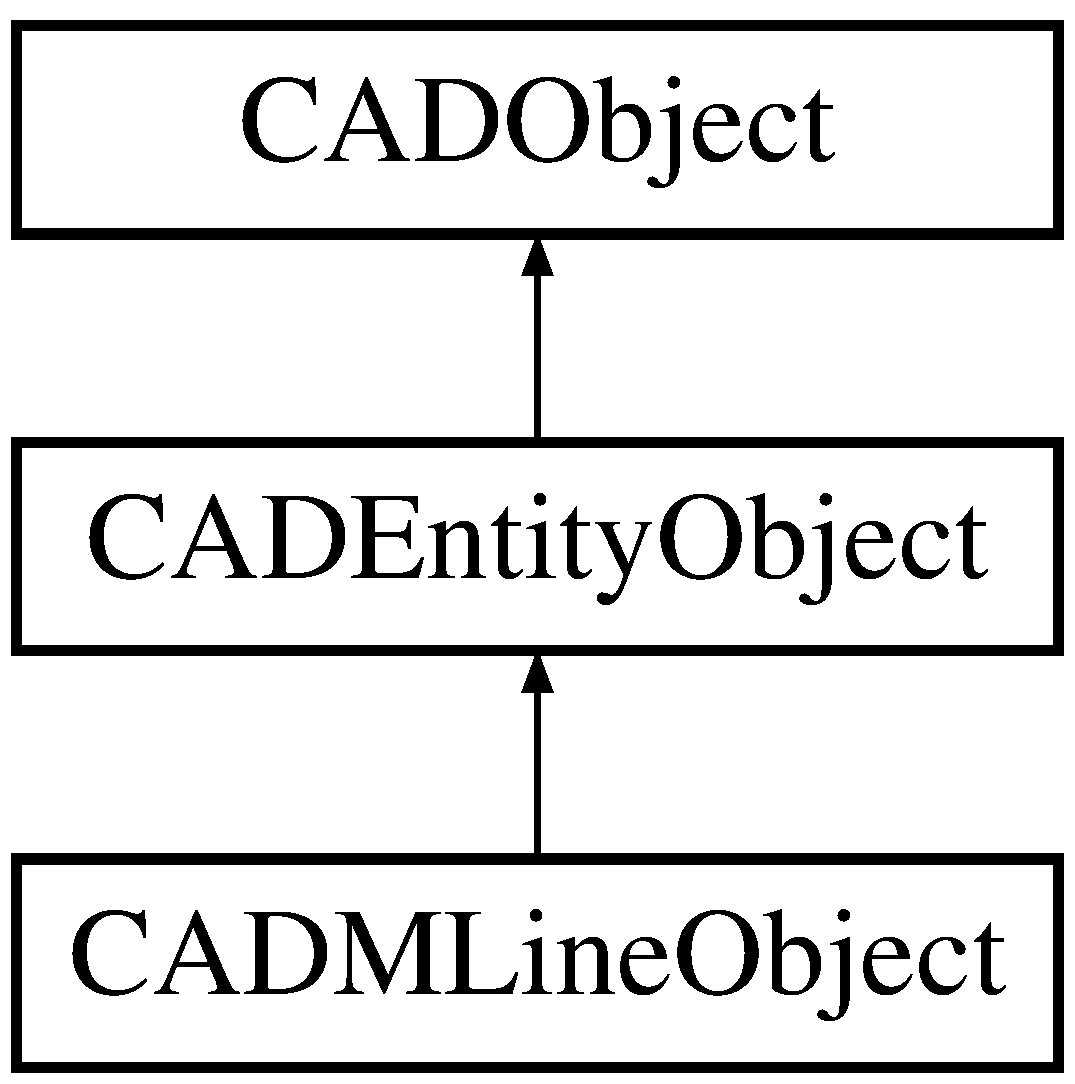
\includegraphics[height=3.000000cm]{class_c_a_d_m_line_object}
\end{center}
\end{figure}
\subsection*{Public Attributes}
\begin{DoxyCompactItemize}
\item 
double {\bfseries df\+Scale}\hypertarget{class_c_a_d_m_line_object_a89af070519c1cd00190ab6d4cb31992f}{}\label{class_c_a_d_m_line_object_a89af070519c1cd00190ab6d4cb31992f}

\item 
unsigned char {\bfseries d\+Just}\hypertarget{class_c_a_d_m_line_object_a836492a72ea38e08ebe334de0fbebe9a}{}\label{class_c_a_d_m_line_object_a836492a72ea38e08ebe334de0fbebe9a}

\item 
\hyperlink{class_c_a_d_vector}{C\+A\+D\+Vector} {\bfseries vert\+Base\+Point}\hypertarget{class_c_a_d_m_line_object_ae25e161b257eb1a57de314377ba247ea}{}\label{class_c_a_d_m_line_object_ae25e161b257eb1a57de314377ba247ea}

\item 
\hyperlink{class_c_a_d_vector}{C\+A\+D\+Vector} {\bfseries vect\+Extrusion}\hypertarget{class_c_a_d_m_line_object_a8add8dd1b87abbc8325d1993640cfffe}{}\label{class_c_a_d_m_line_object_a8add8dd1b87abbc8325d1993640cfffe}

\item 
short {\bfseries d\+Open\+Closed}\hypertarget{class_c_a_d_m_line_object_a190035f9ebc186017d29abcec625b4bc}{}\label{class_c_a_d_m_line_object_a190035f9ebc186017d29abcec625b4bc}

\item 
unsigned char {\bfseries n\+Lines\+In\+Style}\hypertarget{class_c_a_d_m_line_object_a2bc2dc32a7cf14df6861f5488038d2e1}{}\label{class_c_a_d_m_line_object_a2bc2dc32a7cf14df6861f5488038d2e1}

\item 
short {\bfseries n\+Num\+Vertexes}\hypertarget{class_c_a_d_m_line_object_ae8da6b01959d5717122da17bbba3f19b}{}\label{class_c_a_d_m_line_object_ae8da6b01959d5717122da17bbba3f19b}

\item 
vector$<$ \hyperlink{struct__mlinevertex}{C\+A\+D\+M\+Line\+Vertex} $>$ {\bfseries avert\+Vertexes}\hypertarget{class_c_a_d_m_line_object_a1cd3715f0fd989ace24f8b0b1c8c3a33}{}\label{class_c_a_d_m_line_object_a1cd3715f0fd989ace24f8b0b1c8c3a33}

\item 
\hyperlink{class_c_a_d_handle}{C\+A\+D\+Handle} {\bfseries h\+M\+Line\+Style}\hypertarget{class_c_a_d_m_line_object_ad496da713b0f00c25d95c0c547880b18}{}\label{class_c_a_d_m_line_object_ad496da713b0f00c25d95c0c547880b18}

\end{DoxyCompactItemize}
\subsection*{Additional Inherited Members}


\subsection{Detailed Description}
The \hyperlink{class_c_a_d_m_line_object}{C\+A\+D\+M\+Line\+Object} class. 

The documentation for this class was generated from the following files\+:\begin{DoxyCompactItemize}
\item 
cadobjects.\+h\item 
cadobjects.\+cpp\end{DoxyCompactItemize}

\hypertarget{class_c_a_d_m_text}{}\section{C\+A\+D\+M\+Text Class Reference}
\label{class_c_a_d_m_text}\index{C\+A\+D\+M\+Text@{C\+A\+D\+M\+Text}}


Geometry class which represents M\+Text.  




{\ttfamily \#include $<$cadgeometry.\+h$>$}

Inheritance diagram for C\+A\+D\+M\+Text\+:\begin{figure}[H]
\begin{center}
\leavevmode
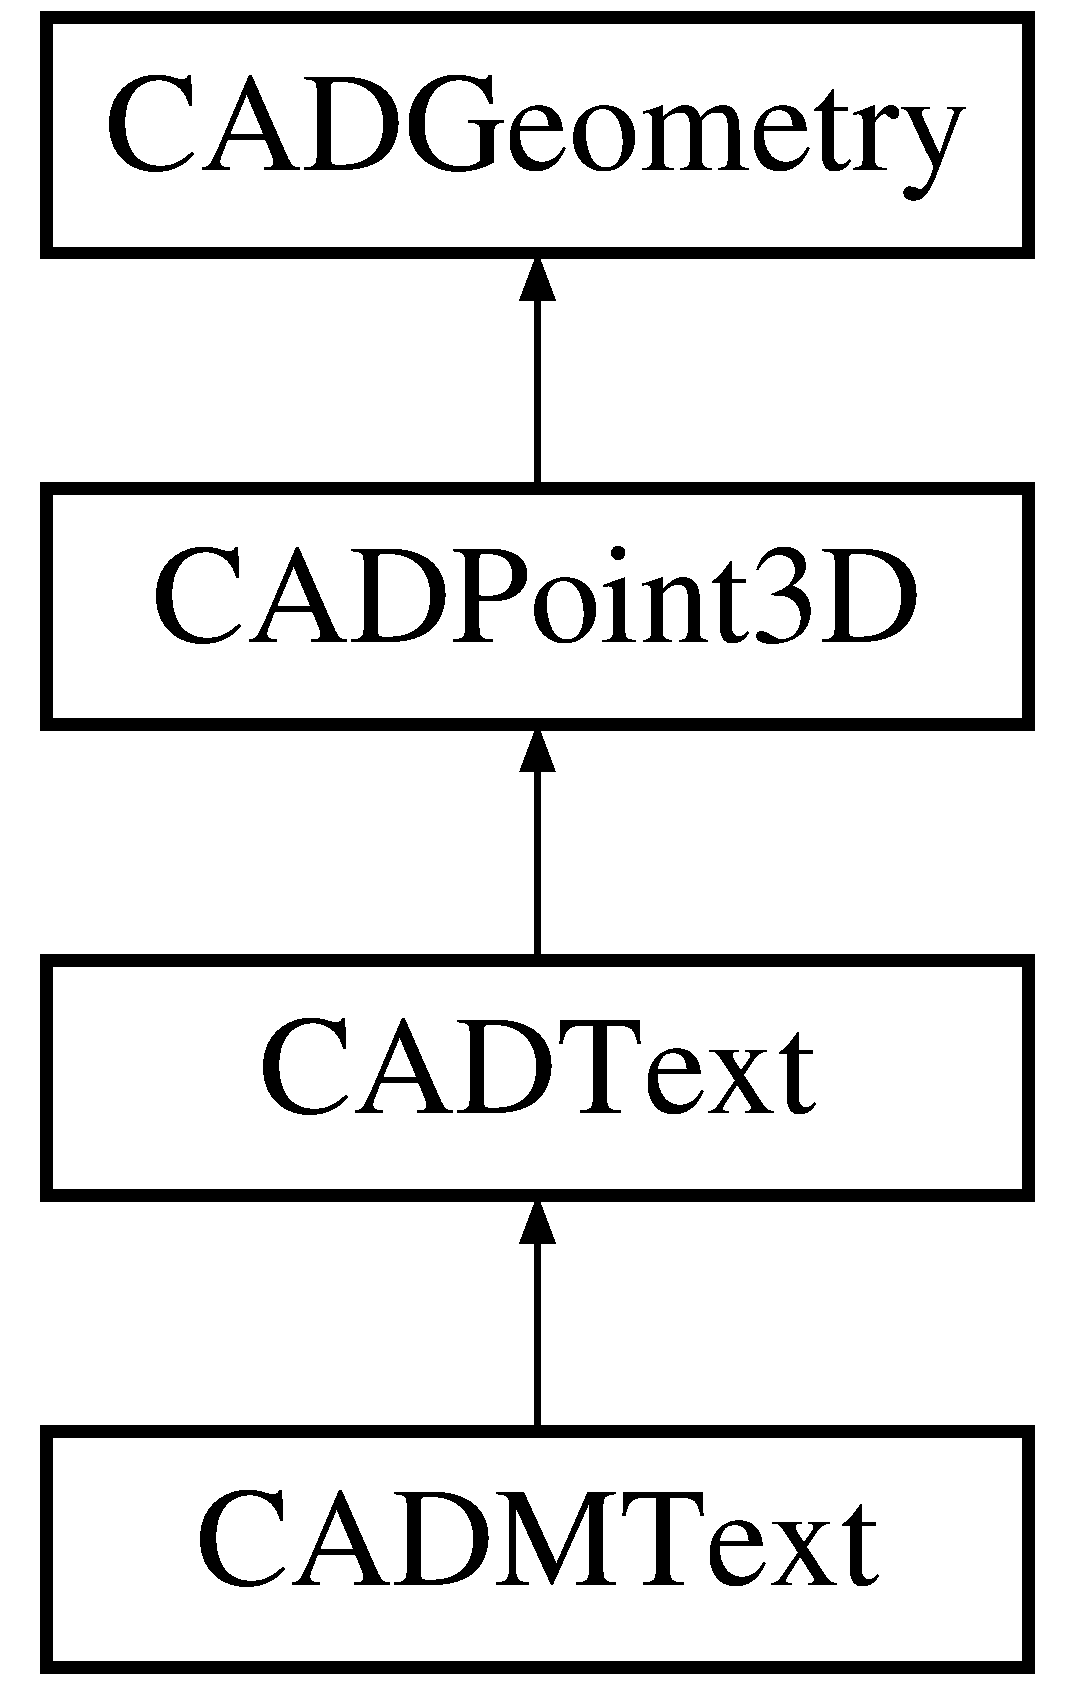
\includegraphics[height=4.000000cm]{class_c_a_d_m_text}
\end{center}
\end{figure}
\subsection*{Public Member Functions}
\begin{DoxyCompactItemize}
\item 
double {\bfseries get\+Rect\+Width} () const \hypertarget{class_c_a_d_m_text_aa96b0a212ae5a028a474724853ec2e99}{}\label{class_c_a_d_m_text_aa96b0a212ae5a028a474724853ec2e99}

\item 
void {\bfseries set\+Rect\+Width} (double value)\hypertarget{class_c_a_d_m_text_ad1d46ca2fcf36dad4cbed184a73276a1}{}\label{class_c_a_d_m_text_ad1d46ca2fcf36dad4cbed184a73276a1}

\item 
double {\bfseries get\+Extents} () const \hypertarget{class_c_a_d_m_text_af98eea6a6750c56e594ab65a40ed0bd4}{}\label{class_c_a_d_m_text_af98eea6a6750c56e594ab65a40ed0bd4}

\item 
void {\bfseries set\+Extents} (double value)\hypertarget{class_c_a_d_m_text_a070aa2106db1d9c7b1c38e0109ef9c62}{}\label{class_c_a_d_m_text_a070aa2106db1d9c7b1c38e0109ef9c62}

\item 
double {\bfseries get\+Extents\+Width} () const \hypertarget{class_c_a_d_m_text_a2169394e64b4fa46ec8b1d5c166beeec}{}\label{class_c_a_d_m_text_a2169394e64b4fa46ec8b1d5c166beeec}

\item 
void {\bfseries set\+Extents\+Width} (double value)\hypertarget{class_c_a_d_m_text_ae439b628a578c5828c250232bcd77fb0}{}\label{class_c_a_d_m_text_ae439b628a578c5828c250232bcd77fb0}

\item 
virtual void {\bfseries print} () const  override\hypertarget{class_c_a_d_m_text_a3de2f102eb782b848f54adc748d55c33}{}\label{class_c_a_d_m_text_a3de2f102eb782b848f54adc748d55c33}

\end{DoxyCompactItemize}
\subsection*{Protected Attributes}
\begin{DoxyCompactItemize}
\item 
double {\bfseries rect\+Width}\hypertarget{class_c_a_d_m_text_abca1c6ffbb45db76b7d51af03fffd52a}{}\label{class_c_a_d_m_text_abca1c6ffbb45db76b7d51af03fffd52a}

\item 
double {\bfseries extents}\hypertarget{class_c_a_d_m_text_af4eb8fd85596249788cf29fc749e3ad1}{}\label{class_c_a_d_m_text_af4eb8fd85596249788cf29fc749e3ad1}

\item 
double {\bfseries extents\+Width}\hypertarget{class_c_a_d_m_text_a1ae61c088810cf81833a65758242dcfd}{}\label{class_c_a_d_m_text_a1ae61c088810cf81833a65758242dcfd}

\end{DoxyCompactItemize}
\subsection*{Additional Inherited Members}


\subsection{Detailed Description}
Geometry class which represents M\+Text. 

The documentation for this class was generated from the following files\+:\begin{DoxyCompactItemize}
\item 
cadgeometry.\+h\item 
cadgeometry.\+cpp\end{DoxyCompactItemize}

\hypertarget{class_c_a_d_m_text_object}{}\section{C\+A\+D\+M\+Text\+Object Class Reference}
\label{class_c_a_d_m_text_object}\index{C\+A\+D\+M\+Text\+Object@{C\+A\+D\+M\+Text\+Object}}


The \hyperlink{class_c_a_d_m_text_object}{C\+A\+D\+M\+Text\+Object} class.  




{\ttfamily \#include $<$cadobjects.\+h$>$}

Inheritance diagram for C\+A\+D\+M\+Text\+Object\+:\begin{figure}[H]
\begin{center}
\leavevmode
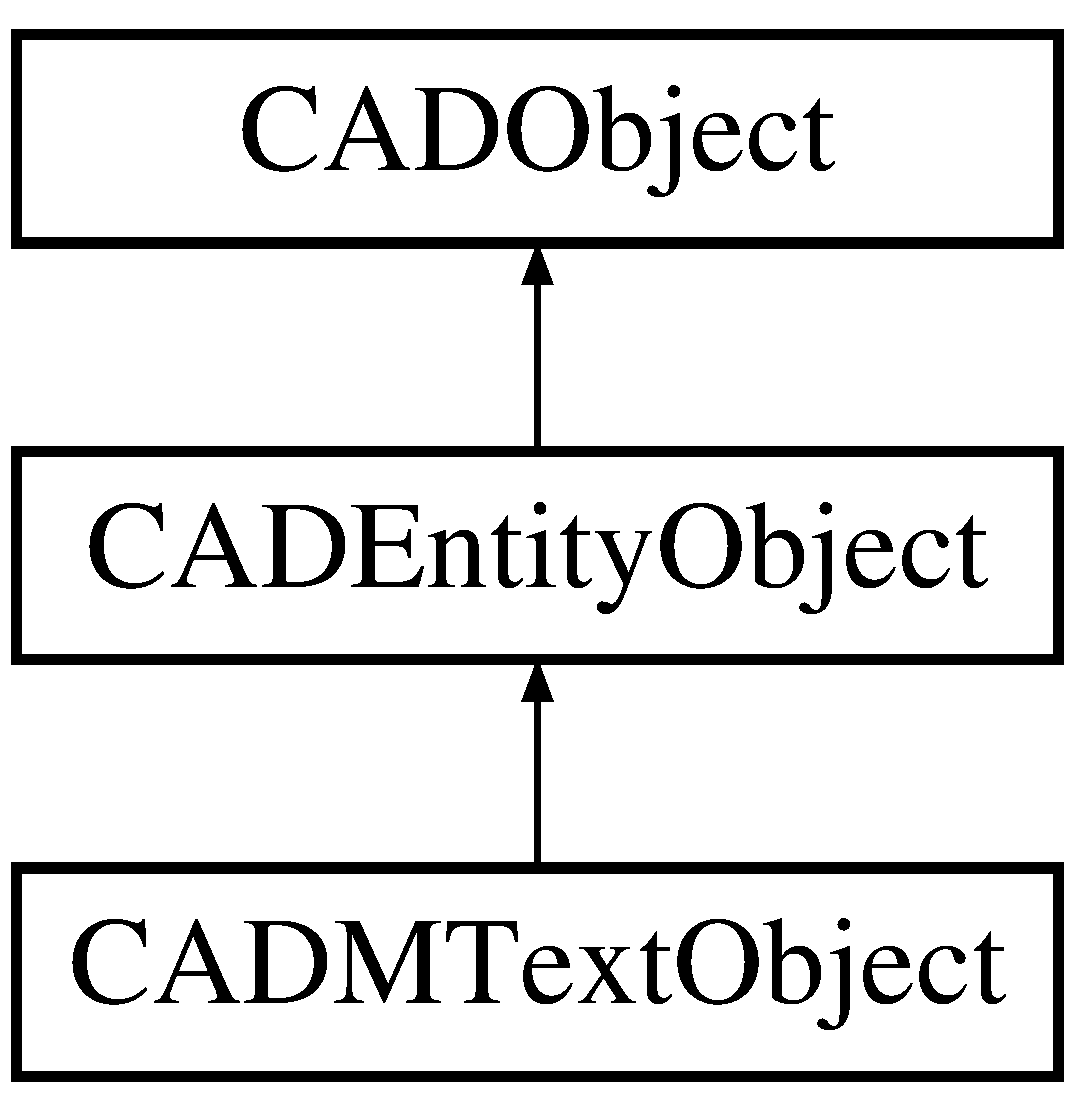
\includegraphics[height=3.000000cm]{class_c_a_d_m_text_object}
\end{center}
\end{figure}
\subsection*{Public Attributes}
\begin{DoxyCompactItemize}
\item 
\hyperlink{class_c_a_d_vector}{C\+A\+D\+Vector} {\bfseries vert\+Insertion\+Point}\hypertarget{class_c_a_d_m_text_object_af0bb24e8e6d30b3439d57d2753cdf7f9}{}\label{class_c_a_d_m_text_object_af0bb24e8e6d30b3439d57d2753cdf7f9}

\item 
\hyperlink{class_c_a_d_vector}{C\+A\+D\+Vector} {\bfseries vect\+Extrusion}\hypertarget{class_c_a_d_m_text_object_a43d93193dfc45453c16706a77b05d1b5}{}\label{class_c_a_d_m_text_object_a43d93193dfc45453c16706a77b05d1b5}

\item 
\hyperlink{class_c_a_d_vector}{C\+A\+D\+Vector} {\bfseries vect\+X\+Axis\+Dir}\hypertarget{class_c_a_d_m_text_object_aa4bcfc479e853f94de1e9ac675f1bb43}{}\label{class_c_a_d_m_text_object_aa4bcfc479e853f94de1e9ac675f1bb43}

\item 
double {\bfseries df\+Rect\+Width}\hypertarget{class_c_a_d_m_text_object_aa1047aa721eef9b9016c99626151e896}{}\label{class_c_a_d_m_text_object_aa1047aa721eef9b9016c99626151e896}

\item 
double {\bfseries df\+Text\+Height}\hypertarget{class_c_a_d_m_text_object_a4b17152ad79e6f2cf1eb6b6af3757012}{}\label{class_c_a_d_m_text_object_a4b17152ad79e6f2cf1eb6b6af3757012}

\item 
short {\bfseries d\+Attachment}\hypertarget{class_c_a_d_m_text_object_ac3d38fef48ba0da1d0b1eeeaa81e90bd}{}\label{class_c_a_d_m_text_object_ac3d38fef48ba0da1d0b1eeeaa81e90bd}

\item 
short {\bfseries d\+Drawing\+Dir}\hypertarget{class_c_a_d_m_text_object_a75a0fe2d3d0749f43b2dd117979a57bf}{}\label{class_c_a_d_m_text_object_a75a0fe2d3d0749f43b2dd117979a57bf}

\item 
double {\bfseries df\+Extents}\hypertarget{class_c_a_d_m_text_object_a96cd529579cf59c74430ab84c0922203}{}\label{class_c_a_d_m_text_object_a96cd529579cf59c74430ab84c0922203}

\item 
double {\bfseries df\+Extents\+Width}\hypertarget{class_c_a_d_m_text_object_ac24e38c41ef1e1352b4ccabd62936656}{}\label{class_c_a_d_m_text_object_ac24e38c41ef1e1352b4ccabd62936656}

\item 
string {\bfseries s\+Text\+Value}\hypertarget{class_c_a_d_m_text_object_a9f924944d10fd0b2fef90dcb4f72a5f3}{}\label{class_c_a_d_m_text_object_a9f924944d10fd0b2fef90dcb4f72a5f3}

\item 
short {\bfseries d\+Line\+Spacing\+Style}\hypertarget{class_c_a_d_m_text_object_af93d432402ad8eac198e1020c6a0092f}{}\label{class_c_a_d_m_text_object_af93d432402ad8eac198e1020c6a0092f}

\item 
double {\bfseries d\+Line\+Spacing\+Factor}\hypertarget{class_c_a_d_m_text_object_a3684f352d80287072c152ba072afd1f4}{}\label{class_c_a_d_m_text_object_a3684f352d80287072c152ba072afd1f4}

\item 
bool {\bfseries b\+Unknown\+Bit}\hypertarget{class_c_a_d_m_text_object_adb504ec2e3fd4e552edbbe9ac932df1c}{}\label{class_c_a_d_m_text_object_adb504ec2e3fd4e552edbbe9ac932df1c}

\item 
long {\bfseries d\+Background\+Flags}\hypertarget{class_c_a_d_m_text_object_ad1015f8d615227c0c5ffe505fe997a47}{}\label{class_c_a_d_m_text_object_ad1015f8d615227c0c5ffe505fe997a47}

\item 
long {\bfseries d\+Background\+Scale\+Factor}\hypertarget{class_c_a_d_m_text_object_afc4d2631c7f82fa62d476303f302c8bb}{}\label{class_c_a_d_m_text_object_afc4d2631c7f82fa62d476303f302c8bb}

\item 
short {\bfseries d\+Background\+Color}\hypertarget{class_c_a_d_m_text_object_af867f24f79e98122a4f3298abd4b8855}{}\label{class_c_a_d_m_text_object_af867f24f79e98122a4f3298abd4b8855}

\item 
long {\bfseries d\+Background\+Transparency}\hypertarget{class_c_a_d_m_text_object_afbcfd1e13d250b1458d75720e747f61e}{}\label{class_c_a_d_m_text_object_afbcfd1e13d250b1458d75720e747f61e}

\item 
\hyperlink{class_c_a_d_handle}{C\+A\+D\+Handle} {\bfseries h\+Style}\hypertarget{class_c_a_d_m_text_object_ab63b8fcdb2852dc4c5a90f30d318fe55}{}\label{class_c_a_d_m_text_object_ab63b8fcdb2852dc4c5a90f30d318fe55}

\end{DoxyCompactItemize}
\subsection*{Additional Inherited Members}


\subsection{Detailed Description}
The \hyperlink{class_c_a_d_m_text_object}{C\+A\+D\+M\+Text\+Object} class. 

The documentation for this class was generated from the following files\+:\begin{DoxyCompactItemize}
\item 
cadobjects.\+h\item 
cadobjects.\+cpp\end{DoxyCompactItemize}

\hypertarget{class_c_a_d_object}{}\section{C\+A\+D\+Object Class Reference}
\label{class_c_a_d_object}\index{C\+A\+D\+Object@{C\+A\+D\+Object}}


The base C\+AD object class.  




{\ttfamily \#include $<$cadobjects.\+h$>$}

Inheritance diagram for C\+A\+D\+Object\+:\begin{figure}[H]
\begin{center}
\leavevmode
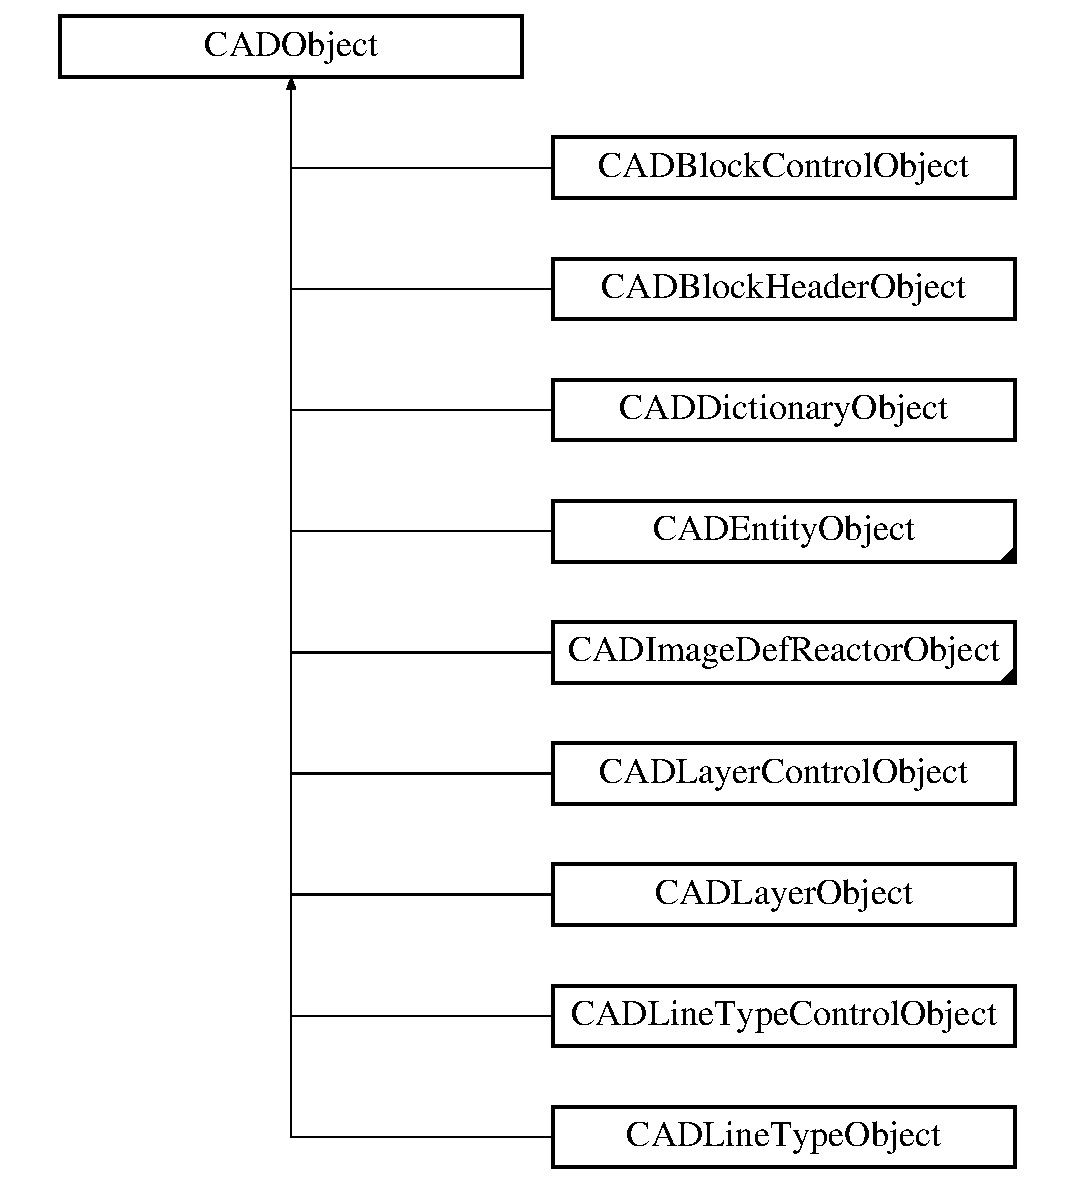
\includegraphics[height=10.000000cm]{class_c_a_d_object}
\end{center}
\end{figure}
\subsection*{Public Types}
\begin{DoxyCompactItemize}
\item 
enum {\bfseries Object\+Type} \{ \\*
{\bfseries U\+N\+U\+S\+ED} = 0x0, 
{\bfseries T\+E\+XT} = 0x1, 
{\bfseries A\+T\+T\+R\+IB} = 0x2, 
{\bfseries A\+T\+T\+D\+EF} = 0x3, 
\\*
{\bfseries B\+L\+O\+CK} = 0x4, 
{\bfseries E\+N\+D\+B\+LK} = 0x5, 
{\bfseries S\+E\+Q\+E\+ND} = 0x6, 
{\bfseries I\+N\+S\+E\+RT} = 0x7, 
\\*
{\bfseries M\+I\+N\+S\+E\+R\+T1} = 0x8, 
{\bfseries M\+I\+N\+S\+E\+R\+T2} = 0x9, 
{\bfseries V\+E\+R\+T\+E\+X2D} = 0x0A, 
{\bfseries V\+E\+R\+T\+E\+X3D} = 0x0B, 
\\*
{\bfseries V\+E\+R\+T\+E\+X\+\_\+\+M\+E\+SH} = 0x0C, 
{\bfseries V\+E\+R\+T\+E\+X\+\_\+\+P\+F\+A\+CE} = 0x0D, 
{\bfseries V\+E\+R\+T\+E\+X\+\_\+\+P\+F\+A\+C\+E\+\_\+\+F\+A\+CE} = 0x0E, 
{\bfseries P\+O\+L\+Y\+L\+I\+N\+E2D} = 0x0F, 
\\*
{\bfseries P\+O\+L\+Y\+L\+I\+N\+E3D} = 0x10, 
{\bfseries A\+RC} = 0x11, 
{\bfseries C\+I\+R\+C\+LE} = 0x12, 
{\bfseries L\+I\+NE} = 0x13, 
\\*
{\bfseries D\+I\+M\+E\+N\+S\+I\+O\+N\+\_\+\+O\+R\+D\+I\+N\+A\+TE} = 0x14, 
{\bfseries D\+I\+M\+E\+N\+S\+I\+O\+N\+\_\+\+L\+I\+N\+E\+AR} = 0x15, 
{\bfseries D\+I\+M\+E\+N\+S\+I\+O\+N\+\_\+\+A\+L\+I\+G\+N\+ED} = 0x16, 
{\bfseries D\+I\+M\+E\+N\+S\+I\+O\+N\+\_\+\+A\+N\+G\+\_\+3\+PT} = 0x17, 
\\*
{\bfseries D\+I\+M\+E\+N\+S\+I\+O\+N\+\_\+\+A\+N\+G\+\_\+2\+LN} = 0x18, 
{\bfseries D\+I\+M\+E\+N\+S\+I\+O\+N\+\_\+\+R\+A\+D\+I\+US} = 0x19, 
{\bfseries D\+I\+M\+E\+N\+S\+I\+O\+N\+\_\+\+D\+I\+A\+M\+E\+T\+ER} = 0x1A, 
{\bfseries P\+O\+I\+NT} = 0x1B, 
\\*
{\bfseries F\+A\+C\+E3D} = 0x1C, 
{\bfseries P\+O\+L\+Y\+L\+I\+N\+E\+\_\+\+P\+F\+A\+CE} = 0x1D, 
{\bfseries P\+O\+L\+Y\+L\+I\+N\+E\+\_\+\+M\+E\+SH} = 0x1E, 
{\bfseries S\+O\+L\+ID} = 0x1F, 
\\*
{\bfseries T\+R\+A\+CE} = 0x20, 
{\bfseries S\+H\+A\+PE} = 0x21, 
{\bfseries V\+I\+E\+W\+P\+O\+RT} = 0x22, 
{\bfseries E\+L\+L\+I\+P\+SE} = 0x23, 
\\*
{\bfseries S\+P\+L\+I\+NE} = 0x24, 
{\bfseries R\+E\+G\+I\+ON} = 0x25, 
{\bfseries S\+O\+L\+I\+D3D} = 0x26, 
{\bfseries B\+O\+DY} = 0x27, 
\\*
{\bfseries R\+AY} = 0x28, 
{\bfseries X\+L\+I\+NE} = 0x29, 
{\bfseries D\+I\+C\+T\+I\+O\+N\+A\+RY} = 0x2A, 
{\bfseries O\+L\+E\+F\+R\+A\+ME} = 0x2B, 
\\*
{\bfseries M\+T\+E\+XT} = 0x2C, 
{\bfseries L\+E\+A\+D\+ER} = 0x2D, 
{\bfseries T\+O\+L\+E\+R\+A\+N\+CE} = 0x2E, 
{\bfseries M\+L\+I\+NE} = 0x2F, 
\\*
{\bfseries B\+L\+O\+C\+K\+\_\+\+C\+O\+N\+T\+R\+O\+L\+\_\+\+O\+BJ} = 0x30, 
{\bfseries B\+L\+O\+C\+K\+\_\+\+H\+E\+A\+D\+ER} = 0x31, 
{\bfseries L\+A\+Y\+E\+R\+\_\+\+C\+O\+N\+T\+R\+O\+L\+\_\+\+O\+BJ} = 0x32, 
{\bfseries L\+A\+Y\+ER} = 0x33, 
\\*
{\bfseries S\+T\+Y\+L\+E\+\_\+\+C\+O\+N\+T\+R\+O\+L\+\_\+\+O\+BJ} = 0x34, 
{\bfseries S\+T\+Y\+L\+E1} = 0x35, 
{\bfseries S\+T\+Y\+L\+E2} = 0x36, 
{\bfseries S\+T\+Y\+L\+E3} = 0x37, 
\\*
{\bfseries L\+T\+Y\+P\+E\+\_\+\+C\+O\+N\+T\+R\+O\+L\+\_\+\+O\+BJ} = 0x38, 
{\bfseries L\+T\+Y\+P\+E1} = 0x39, 
{\bfseries L\+T\+Y\+P\+E2} = 0x3A, 
{\bfseries L\+T\+Y\+P\+E3} = 0x3B, 
\\*
{\bfseries V\+I\+E\+W\+\_\+\+C\+O\+N\+T\+R\+O\+L\+\_\+\+O\+BJ} = 0x3C, 
{\bfseries V\+I\+EW} = 0x3D, 
{\bfseries U\+C\+S\+\_\+\+C\+O\+N\+T\+R\+O\+L\+\_\+\+O\+BJ} = 0x3E, 
{\bfseries U\+CS} = 0x3F, 
\\*
{\bfseries V\+P\+O\+R\+T\+\_\+\+C\+O\+N\+T\+R\+O\+L\+\_\+\+O\+BJ} = 0x40, 
{\bfseries V\+P\+O\+RT} = 0x41, 
{\bfseries A\+P\+P\+I\+D\+\_\+\+C\+O\+N\+T\+R\+O\+L\+\_\+\+O\+BJ} = 0x42, 
{\bfseries A\+P\+P\+ID} = 0x43, 
\\*
{\bfseries D\+I\+M\+S\+T\+Y\+L\+E\+\_\+\+C\+O\+N\+T\+R\+O\+L\+\_\+\+O\+BJ} = 0x44, 
{\bfseries D\+I\+M\+S\+T\+Y\+LE} = 0x45, 
{\bfseries V\+P\+\_\+\+E\+N\+T\+\_\+\+H\+D\+R\+\_\+\+C\+T\+R\+L\+\_\+\+O\+BJ} = 0x46, 
{\bfseries V\+P\+\_\+\+E\+N\+T\+\_\+\+H\+DR} = 0x47, 
\\*
{\bfseries G\+R\+O\+UP} = 0x48, 
{\bfseries M\+L\+I\+N\+E\+S\+T\+Y\+LE} = 0x49, 
{\bfseries O\+L\+E2\+F\+R\+A\+ME} = 0x4A, 
{\bfseries D\+U\+M\+MY} = 0x4B, 
\\*
{\bfseries L\+O\+N\+G\+\_\+\+T\+R\+A\+N\+S\+A\+C\+T\+I\+ON} = 0x4C, 
{\bfseries L\+W\+P\+O\+L\+Y\+L\+I\+NE} = 0x4D, 
{\bfseries H\+A\+T\+CH} = 0x4E, 
{\bfseries X\+R\+E\+C\+O\+RD} = 0x4F, 
\\*
{\bfseries A\+C\+D\+B\+P\+L\+A\+C\+E\+H\+O\+L\+D\+ER} = 0x50, 
{\bfseries V\+B\+A\+\_\+\+P\+R\+O\+J\+E\+CT} = 0x51, 
{\bfseries L\+A\+Y\+O\+UT} = 0x52, 
{\bfseries C\+E\+L\+L\+S\+T\+Y\+L\+E\+M\+AP} = 0x53, 
\\*
{\bfseries D\+B\+C\+O\+L\+OR} = 0x54, 
{\bfseries D\+I\+C\+T\+I\+O\+N\+A\+R\+Y\+V\+AR} = 0x55, 
{\bfseries D\+I\+C\+T\+I\+O\+N\+A\+R\+Y\+W\+D\+F\+LT} = 0x56, 
{\bfseries F\+I\+E\+LD} = 0x57, 
\\*
{\bfseries G\+R\+O\+U\+P\+\_\+\+U\+N\+F\+I\+X\+ED} = 0x58, 
{\bfseries H\+A\+T\+C\+H\+\_\+\+U\+N\+F\+I\+X\+ED} = 0x59, 
{\bfseries I\+D\+B\+U\+F\+F\+ER} = 0x5A, 
{\bfseries I\+M\+A\+GE} = 0x5B, 
\\*
{\bfseries I\+M\+A\+G\+E\+D\+EF} = 0x5C, 
{\bfseries I\+M\+A\+G\+E\+D\+E\+F\+R\+E\+A\+C\+T\+OR} = 0x5D, 
{\bfseries L\+A\+Y\+E\+R\+\_\+\+I\+N\+D\+EX} = 0x5E, 
{\bfseries L\+A\+Y\+O\+U\+T\+\_\+\+U\+N\+F\+I\+X\+ED} = 0x5F, 
\\*
{\bfseries L\+W\+P\+O\+L\+Y\+L\+I\+N\+E\+\_\+\+U\+N\+F\+I\+X\+ED} = 0x60, 
{\bfseries M\+A\+T\+E\+R\+I\+AL} = 0x61, 
{\bfseries M\+L\+E\+A\+D\+ER} = 0x62, 
{\bfseries M\+L\+E\+A\+D\+E\+R\+S\+T\+Y\+LE} = 0x63, 
\\*
{\bfseries O\+L\+E2\+F\+R\+A\+M\+E\+\_\+\+U\+N\+F\+I\+X\+ED} = 0x64, 
{\bfseries P\+L\+A\+C\+E\+H\+O\+L\+D\+ER} = 0x65, 
{\bfseries P\+L\+O\+T\+S\+E\+T\+T\+I\+N\+GS} = 0x66, 
{\bfseries R\+A\+S\+T\+E\+R\+V\+A\+R\+I\+A\+B\+L\+ES} = 0x67, 
\\*
{\bfseries S\+C\+A\+LE} = 0x68, 
{\bfseries S\+O\+R\+T\+E\+N\+T\+S\+T\+A\+B\+LE} = 0x69, 
{\bfseries S\+P\+A\+T\+I\+A\+L\+\_\+\+F\+I\+L\+T\+ER} = 0x6A, 
{\bfseries S\+P\+A\+T\+I\+A\+L\+\_\+\+I\+N\+D\+EX} = 0x6B, 
\\*
{\bfseries T\+A\+B\+L\+E\+G\+E\+O\+M\+E\+T\+RY} = 0x6C, 
{\bfseries T\+A\+B\+L\+E\+S\+T\+Y\+L\+ES} = 0x6D, 
{\bfseries V\+B\+A\+\_\+\+P\+R\+O\+J\+E\+C\+T\+\_\+\+U\+N\+F\+I\+X\+ED} = 0x6E, 
{\bfseries V\+I\+S\+U\+A\+L\+S\+T\+Y\+LE} = 0x6F, 
\\*
{\bfseries W\+I\+P\+E\+O\+U\+T\+V\+A\+R\+I\+A\+B\+LE} = 0x70, 
{\bfseries X\+R\+E\+C\+O\+R\+D\+\_\+\+U\+N\+F\+I\+X\+ED} = 0x71
 \}\hypertarget{class_c_a_d_object_a9db91e0070823b565bf904ac8bc52194}{}\label{class_c_a_d_object_a9db91e0070823b565bf904ac8bc52194}

\end{DoxyCompactItemize}
\subsection*{Public Member Functions}
\begin{DoxyCompactItemize}
\item 
Object\+Type {\bfseries get\+Type} () const \hypertarget{class_c_a_d_object_aeb28c49575260e805dcb6e89bcab66d1}{}\label{class_c_a_d_object_aeb28c49575260e805dcb6e89bcab66d1}

\item 
long {\bfseries get\+Size} () const \hypertarget{class_c_a_d_object_a8804309e9a149fbabfd154b66ed1cdc6}{}\label{class_c_a_d_object_a8804309e9a149fbabfd154b66ed1cdc6}

\item 
void {\bfseries set\+Size} (long value)\hypertarget{class_c_a_d_object_abf6a52a76f5bedee3a821dab283d6be5}{}\label{class_c_a_d_object_abf6a52a76f5bedee3a821dab283d6be5}

\item 
void {\bfseries set\+Type} (const Object\+Type \&value)\hypertarget{class_c_a_d_object_aadba6a4e9cc766c22f8d3293fd34f053}{}\label{class_c_a_d_object_aadba6a4e9cc766c22f8d3293fd34f053}

\item 
short {\bfseries get\+C\+RC} () const \hypertarget{class_c_a_d_object_aeb42f23220a144dc8de8c70ba61dfa64}{}\label{class_c_a_d_object_aeb42f23220a144dc8de8c70ba61dfa64}

\item 
void {\bfseries set\+C\+RC} (short value)\hypertarget{class_c_a_d_object_abc58fdb22314817f2d5adc32b8cb5686}{}\label{class_c_a_d_object_abc58fdb22314817f2d5adc32b8cb5686}

\end{DoxyCompactItemize}
\subsection*{Protected Attributes}
\begin{DoxyCompactItemize}
\item 
long {\bfseries size}\hypertarget{class_c_a_d_object_a306f110c0f5e623796dddfd89c639501}{}\label{class_c_a_d_object_a306f110c0f5e623796dddfd89c639501}

\item 
Object\+Type {\bfseries type}\hypertarget{class_c_a_d_object_a6f467edf5a0fc2ed5e6b48d583623c2e}{}\label{class_c_a_d_object_a6f467edf5a0fc2ed5e6b48d583623c2e}

\item 
short {\bfseries C\+RC}\hypertarget{class_c_a_d_object_ab7af653f9c40a8de82f3a99cd705c6ae}{}\label{class_c_a_d_object_ab7af653f9c40a8de82f3a99cd705c6ae}

\end{DoxyCompactItemize}


\subsection{Detailed Description}
The base C\+AD object class. 

The documentation for this class was generated from the following files\+:\begin{DoxyCompactItemize}
\item 
cadobjects.\+h\item 
cadobjects.\+cpp\end{DoxyCompactItemize}

\hypertarget{class_c_a_d_point3_d}{}\section{C\+A\+D\+Point3D Class Reference}
\label{class_c_a_d_point3_d}\index{C\+A\+D\+Point3D@{C\+A\+D\+Point3D}}


Geometry class which a single Point.  




{\ttfamily \#include $<$cadgeometry.\+h$>$}

Inheritance diagram for C\+A\+D\+Point3D\+:\begin{figure}[H]
\begin{center}
\leavevmode
\includegraphics[height=5.000000cm]{class_c_a_d_point3_d}
\end{center}
\end{figure}
\subsection*{Public Member Functions}
\begin{DoxyCompactItemize}
\item 
{\bfseries C\+A\+D\+Point3D} (const \hyperlink{class_c_a_d_vector}{C\+A\+D\+Vector} \&position\+In, double thickness\+In)\hypertarget{class_c_a_d_point3_d_a2b90070589b8f309581c7ce40154b492}{}\label{class_c_a_d_point3_d_a2b90070589b8f309581c7ce40154b492}

\item 
\hyperlink{class_c_a_d_vector}{C\+A\+D\+Vector} {\bfseries get\+Position} () const \hypertarget{class_c_a_d_point3_d_a82f9c92dd7ef5e927993e69e83279e5e}{}\label{class_c_a_d_point3_d_a82f9c92dd7ef5e927993e69e83279e5e}

\item 
void {\bfseries set\+Position} (const \hyperlink{class_c_a_d_vector}{C\+A\+D\+Vector} \&value)\hypertarget{class_c_a_d_point3_d_a46a65c6b3466d9dca9e0827b011f418e}{}\label{class_c_a_d_point3_d_a46a65c6b3466d9dca9e0827b011f418e}

\item 
\hyperlink{class_c_a_d_vector}{C\+A\+D\+Vector} {\bfseries get\+Extrusion} () const \hypertarget{class_c_a_d_point3_d_ae1ab182fd97f2317c50c7dac4931f1d3}{}\label{class_c_a_d_point3_d_ae1ab182fd97f2317c50c7dac4931f1d3}

\item 
void {\bfseries set\+Extrusion} (const \hyperlink{class_c_a_d_vector}{C\+A\+D\+Vector} \&value)\hypertarget{class_c_a_d_point3_d_adb460d9f84c10c14967d61807740abdc}{}\label{class_c_a_d_point3_d_adb460d9f84c10c14967d61807740abdc}

\item 
double {\bfseries get\+X\+Axis\+Ang} () const \hypertarget{class_c_a_d_point3_d_a1dfcad378f108a7022c5ffd5c357d631}{}\label{class_c_a_d_point3_d_a1dfcad378f108a7022c5ffd5c357d631}

\item 
void {\bfseries set\+X\+Axis\+Ang} (double value)\hypertarget{class_c_a_d_point3_d_a9b24c0bbe8a41c5cbb07a704cb5c74e9}{}\label{class_c_a_d_point3_d_a9b24c0bbe8a41c5cbb07a704cb5c74e9}

\item 
virtual void {\bfseries print} () const  override\hypertarget{class_c_a_d_point3_d_a5a6bb085f069b7c93488f0ea442fdd29}{}\label{class_c_a_d_point3_d_a5a6bb085f069b7c93488f0ea442fdd29}

\end{DoxyCompactItemize}
\subsection*{Protected Attributes}
\begin{DoxyCompactItemize}
\item 
\hyperlink{class_c_a_d_vector}{C\+A\+D\+Vector} {\bfseries position}\hypertarget{class_c_a_d_point3_d_a0ebb31ec5b9d7744849099d4f618f0f4}{}\label{class_c_a_d_point3_d_a0ebb31ec5b9d7744849099d4f618f0f4}

\item 
\hyperlink{class_c_a_d_vector}{C\+A\+D\+Vector} {\bfseries extrusion}\hypertarget{class_c_a_d_point3_d_a6d4e4c354ce97bd62c9db60feb3c74f9}{}\label{class_c_a_d_point3_d_a6d4e4c354ce97bd62c9db60feb3c74f9}

\item 
double {\bfseries x\+Axis\+Ang}\hypertarget{class_c_a_d_point3_d_a351cfb9e2f3dd6e74b2ba1746ce5d174}{}\label{class_c_a_d_point3_d_a351cfb9e2f3dd6e74b2ba1746ce5d174}

\end{DoxyCompactItemize}
\subsection*{Additional Inherited Members}


\subsection{Detailed Description}
Geometry class which a single Point. 

The documentation for this class was generated from the following files\+:\begin{DoxyCompactItemize}
\item 
cadgeometry.\+h\item 
cadgeometry.\+cpp\end{DoxyCompactItemize}

\hypertarget{class_c_a_d_point_object}{}\section{C\+A\+D\+Point\+Object Class Reference}
\label{class_c_a_d_point_object}\index{C\+A\+D\+Point\+Object@{C\+A\+D\+Point\+Object}}


The \hyperlink{class_c_a_d_point_object}{C\+A\+D\+Point\+Object} class.  




{\ttfamily \#include $<$cadobjects.\+h$>$}

Inheritance diagram for C\+A\+D\+Point\+Object\+:\begin{figure}[H]
\begin{center}
\leavevmode
\includegraphics[height=3.000000cm]{class_c_a_d_point_object}
\end{center}
\end{figure}
\subsection*{Public Attributes}
\begin{DoxyCompactItemize}
\item 
\hyperlink{class_c_a_d_vector}{C\+A\+D\+Vector} {\bfseries vert\+Position}\hypertarget{class_c_a_d_point_object_a16ef3ec7b39f839b9306a55030bdc9e1}{}\label{class_c_a_d_point_object_a16ef3ec7b39f839b9306a55030bdc9e1}

\item 
double {\bfseries df\+Thickness}\hypertarget{class_c_a_d_point_object_a426a51a6aab35e4ff94eed1cfb84e90c}{}\label{class_c_a_d_point_object_a426a51a6aab35e4ff94eed1cfb84e90c}

\item 
\hyperlink{class_c_a_d_vector}{C\+A\+D\+Vector} {\bfseries vect\+Extrusion}\hypertarget{class_c_a_d_point_object_a8d1aeb32e255999dc87cc62beda52fe9}{}\label{class_c_a_d_point_object_a8d1aeb32e255999dc87cc62beda52fe9}

\item 
double {\bfseries df\+X\+Axis\+Ang}\hypertarget{class_c_a_d_point_object_aee7723e53b1a8ef3a1a1eda36775a32e}{}\label{class_c_a_d_point_object_aee7723e53b1a8ef3a1a1eda36775a32e}

\end{DoxyCompactItemize}
\subsection*{Additional Inherited Members}


\subsection{Detailed Description}
The \hyperlink{class_c_a_d_point_object}{C\+A\+D\+Point\+Object} class. 

The documentation for this class was generated from the following files\+:\begin{DoxyCompactItemize}
\item 
cadobjects.\+h\item 
cadobjects.\+cpp\end{DoxyCompactItemize}

\hypertarget{class_c_a_d_polyline2_d_object}{}\section{C\+A\+D\+Polyline2\+D\+Object Class Reference}
\label{class_c_a_d_polyline2_d_object}\index{C\+A\+D\+Polyline2\+D\+Object@{C\+A\+D\+Polyline2\+D\+Object}}


The \hyperlink{class_c_a_d_polyline2_d_object}{C\+A\+D\+Polyline2\+D\+Object} class.  




{\ttfamily \#include $<$cadobjects.\+h$>$}

Inheritance diagram for C\+A\+D\+Polyline2\+D\+Object\+:\begin{figure}[H]
\begin{center}
\leavevmode
\includegraphics[height=3.000000cm]{class_c_a_d_polyline2_d_object}
\end{center}
\end{figure}
\subsection*{Public Attributes}
\begin{DoxyCompactItemize}
\item 
short {\bfseries d\+Flags}\hypertarget{class_c_a_d_polyline2_d_object_a06b3d07bad255a3d713af103a5aec45a}{}\label{class_c_a_d_polyline2_d_object_a06b3d07bad255a3d713af103a5aec45a}

\item 
short {\bfseries d\+Curve\+N\+Smooth\+Surf\+Type}\hypertarget{class_c_a_d_polyline2_d_object_a72dd6376ea0066566c27c553e4b3c810}{}\label{class_c_a_d_polyline2_d_object_a72dd6376ea0066566c27c553e4b3c810}

\item 
double {\bfseries df\+Start\+Width}\hypertarget{class_c_a_d_polyline2_d_object_a239d7eccf06939c1d97d511dcaa4836a}{}\label{class_c_a_d_polyline2_d_object_a239d7eccf06939c1d97d511dcaa4836a}

\item 
double {\bfseries df\+End\+Width}\hypertarget{class_c_a_d_polyline2_d_object_a28afa751edb86032745eb6eec4806370}{}\label{class_c_a_d_polyline2_d_object_a28afa751edb86032745eb6eec4806370}

\item 
double {\bfseries df\+Thickness}\hypertarget{class_c_a_d_polyline2_d_object_ac0d696fde40be5935e3c5c8c2e816022}{}\label{class_c_a_d_polyline2_d_object_ac0d696fde40be5935e3c5c8c2e816022}

\item 
double {\bfseries df\+Elevation}\hypertarget{class_c_a_d_polyline2_d_object_a58b6961941ff8f8d8e255dd92d05986f}{}\label{class_c_a_d_polyline2_d_object_a58b6961941ff8f8d8e255dd92d05986f}

\item 
\hyperlink{class_c_a_d_vector}{C\+A\+D\+Vector} {\bfseries vect\+Extrusion}\hypertarget{class_c_a_d_polyline2_d_object_a687721a2f72e3cec97fd37dbad53c818}{}\label{class_c_a_d_polyline2_d_object_a687721a2f72e3cec97fd37dbad53c818}

\item 
long {\bfseries n\+Objects\+Owned}\hypertarget{class_c_a_d_polyline2_d_object_a2d2abfa25c984665d29f5f22714e3b3c}{}\label{class_c_a_d_polyline2_d_object_a2d2abfa25c984665d29f5f22714e3b3c}

\item 
C\+A\+D\+Handle\+Array {\bfseries h\+Vertexes}\hypertarget{class_c_a_d_polyline2_d_object_aee3b69f83694366f49e5d6f9461ce111}{}\label{class_c_a_d_polyline2_d_object_aee3b69f83694366f49e5d6f9461ce111}

\item 
\hyperlink{class_c_a_d_handle}{C\+A\+D\+Handle} {\bfseries h\+Seqend}\hypertarget{class_c_a_d_polyline2_d_object_a86c6dc4da3b733a3ef7ef94a14bebb0c}{}\label{class_c_a_d_polyline2_d_object_a86c6dc4da3b733a3ef7ef94a14bebb0c}

\end{DoxyCompactItemize}
\subsection*{Additional Inherited Members}


\subsection{Detailed Description}
The \hyperlink{class_c_a_d_polyline2_d_object}{C\+A\+D\+Polyline2\+D\+Object} class. 

The documentation for this class was generated from the following files\+:\begin{DoxyCompactItemize}
\item 
cadobjects.\+h\item 
cadobjects.\+cpp\end{DoxyCompactItemize}

\hypertarget{class_c_a_d_polyline3_d}{}\section{C\+A\+D\+Polyline3D Class Reference}
\label{class_c_a_d_polyline3_d}\index{C\+A\+D\+Polyline3D@{C\+A\+D\+Polyline3D}}


Geometry class which represents Polyline 3D.  




{\ttfamily \#include $<$cadgeometry.\+h$>$}

Inheritance diagram for C\+A\+D\+Polyline3D\+:\begin{figure}[H]
\begin{center}
\leavevmode
\includegraphics[height=3.000000cm]{class_c_a_d_polyline3_d}
\end{center}
\end{figure}
\subsection*{Public Member Functions}
\begin{DoxyCompactItemize}
\item 
void {\bfseries add\+Vertex} (const \hyperlink{class_c_a_d_vector}{C\+A\+D\+Vector} \&vertex)\hypertarget{class_c_a_d_polyline3_d_a0b9a95bbd8d2827620c73f8de71fe371}{}\label{class_c_a_d_polyline3_d_a0b9a95bbd8d2827620c73f8de71fe371}

\item 
size\+\_\+t {\bfseries get\+Vertex\+Count} () const \hypertarget{class_c_a_d_polyline3_d_a95fa0ffcd115e7a0f45e0cd971f3d33f}{}\label{class_c_a_d_polyline3_d_a95fa0ffcd115e7a0f45e0cd971f3d33f}

\item 
\hyperlink{class_c_a_d_vector}{C\+A\+D\+Vector} \& {\bfseries get\+Vertex} (size\+\_\+t index)\hypertarget{class_c_a_d_polyline3_d_ae712c16461fae14a39c874beec0d0cdf}{}\label{class_c_a_d_polyline3_d_ae712c16461fae14a39c874beec0d0cdf}

\item 
virtual void {\bfseries print} () const  override\hypertarget{class_c_a_d_polyline3_d_a76faf32680a6486e2115970143df2900}{}\label{class_c_a_d_polyline3_d_a76faf32680a6486e2115970143df2900}

\end{DoxyCompactItemize}
\subsection*{Protected Attributes}
\begin{DoxyCompactItemize}
\item 
vector$<$ \hyperlink{class_c_a_d_vector}{C\+A\+D\+Vector} $>$ {\bfseries vertexes}\hypertarget{class_c_a_d_polyline3_d_a29e6b837c98234b4ac27f063855e3688}{}\label{class_c_a_d_polyline3_d_a29e6b837c98234b4ac27f063855e3688}

\end{DoxyCompactItemize}
\subsection*{Additional Inherited Members}


\subsection{Detailed Description}
Geometry class which represents Polyline 3D. 

The documentation for this class was generated from the following files\+:\begin{DoxyCompactItemize}
\item 
cadgeometry.\+h\item 
cadgeometry.\+cpp\end{DoxyCompactItemize}

\hypertarget{class_c_a_d_polyline3_d_object}{}\section{C\+A\+D\+Polyline3\+D\+Object Class Reference}
\label{class_c_a_d_polyline3_d_object}\index{C\+A\+D\+Polyline3\+D\+Object@{C\+A\+D\+Polyline3\+D\+Object}}


The \hyperlink{class_c_a_d_polyline3_d_object}{C\+A\+D\+Polyline3\+D\+Object} class.  




{\ttfamily \#include $<$cadobjects.\+h$>$}

Inheritance diagram for C\+A\+D\+Polyline3\+D\+Object\+:\begin{figure}[H]
\begin{center}
\leavevmode
\includegraphics[height=3.000000cm]{class_c_a_d_polyline3_d_object}
\end{center}
\end{figure}
\subsection*{Public Attributes}
\begin{DoxyCompactItemize}
\item 
unsigned char {\bfseries Splined\+Flags}\hypertarget{class_c_a_d_polyline3_d_object_a064001f6e2f90b3353e3ce41d6142079}{}\label{class_c_a_d_polyline3_d_object_a064001f6e2f90b3353e3ce41d6142079}

\item 
unsigned char {\bfseries Closed\+Flags}\hypertarget{class_c_a_d_polyline3_d_object_a416329b6ed16e4a8b780bc7743c50aa7}{}\label{class_c_a_d_polyline3_d_object_a416329b6ed16e4a8b780bc7743c50aa7}

\item 
long {\bfseries n\+Objects\+Owned}\hypertarget{class_c_a_d_polyline3_d_object_a01da80ee82396bdaf2d63372cda6d4db}{}\label{class_c_a_d_polyline3_d_object_a01da80ee82396bdaf2d63372cda6d4db}

\item 
C\+A\+D\+Handle\+Array {\bfseries h\+Vertexes}\hypertarget{class_c_a_d_polyline3_d_object_abc707d36558de2a3436ea11ccb407f11}{}\label{class_c_a_d_polyline3_d_object_abc707d36558de2a3436ea11ccb407f11}

\item 
\hyperlink{class_c_a_d_handle}{C\+A\+D\+Handle} {\bfseries h\+Seqend}\hypertarget{class_c_a_d_polyline3_d_object_a617db6737f650841b8a4bca01fde9537}{}\label{class_c_a_d_polyline3_d_object_a617db6737f650841b8a4bca01fde9537}

\end{DoxyCompactItemize}
\subsection*{Additional Inherited Members}


\subsection{Detailed Description}
The \hyperlink{class_c_a_d_polyline3_d_object}{C\+A\+D\+Polyline3\+D\+Object} class. 

The documentation for this class was generated from the following files\+:\begin{DoxyCompactItemize}
\item 
cadobjects.\+h\item 
cadobjects.\+cpp\end{DoxyCompactItemize}

\hypertarget{class_c_a_d_polyline_p_face}{}\section{C\+A\+D\+Polyline\+P\+Face Class Reference}
\label{class_c_a_d_polyline_p_face}\index{C\+A\+D\+Polyline\+P\+Face@{C\+A\+D\+Polyline\+P\+Face}}


Geometry class which represents Polyline (P\+Face)  




{\ttfamily \#include $<$cadgeometry.\+h$>$}

Inheritance diagram for C\+A\+D\+Polyline\+P\+Face\+:\begin{figure}[H]
\begin{center}
\leavevmode
\includegraphics[height=2.000000cm]{class_c_a_d_polyline_p_face}
\end{center}
\end{figure}
\subsection*{Public Member Functions}
\begin{DoxyCompactItemize}
\item 
virtual void {\bfseries print} () const  override\hypertarget{class_c_a_d_polyline_p_face_a0215a825620746b040d2773b4504052d}{}\label{class_c_a_d_polyline_p_face_a0215a825620746b040d2773b4504052d}

\item 
void {\bfseries add\+Vertex} (const \hyperlink{class_c_a_d_vector}{C\+A\+D\+Vector} \&vertex)\hypertarget{class_c_a_d_polyline_p_face_ab43e61b8671cac0a878f856edefc6d7f}{}\label{class_c_a_d_polyline_p_face_ab43e61b8671cac0a878f856edefc6d7f}

\end{DoxyCompactItemize}
\subsection*{Protected Attributes}
\begin{DoxyCompactItemize}
\item 
vector$<$ \hyperlink{class_c_a_d_vector}{C\+A\+D\+Vector} $>$ {\bfseries vertexes}\hypertarget{class_c_a_d_polyline_p_face_a4f41b8736cf5548288a64c6867cc6886}{}\label{class_c_a_d_polyline_p_face_a4f41b8736cf5548288a64c6867cc6886}

\end{DoxyCompactItemize}
\subsection*{Additional Inherited Members}


\subsection{Detailed Description}
Geometry class which represents Polyline (P\+Face) 

The documentation for this class was generated from the following files\+:\begin{DoxyCompactItemize}
\item 
cadgeometry.\+h\item 
cadgeometry.\+cpp\end{DoxyCompactItemize}

\hypertarget{class_c_a_d_polyline_p_face_object}{}\section{C\+A\+D\+Polyline\+P\+Face\+Object Class Reference}
\label{class_c_a_d_polyline_p_face_object}\index{C\+A\+D\+Polyline\+P\+Face\+Object@{C\+A\+D\+Polyline\+P\+Face\+Object}}


The \hyperlink{class_c_a_d_polyline_p_face_object}{C\+A\+D\+Polyline\+P\+Face\+Object} class.  




{\ttfamily \#include $<$cadobjects.\+h$>$}

Inheritance diagram for C\+A\+D\+Polyline\+P\+Face\+Object\+:\begin{figure}[H]
\begin{center}
\leavevmode
\includegraphics[height=3.000000cm]{class_c_a_d_polyline_p_face_object}
\end{center}
\end{figure}
\subsection*{Public Attributes}
\begin{DoxyCompactItemize}
\item 
short {\bfseries n\+Num\+Vertexes}\hypertarget{class_c_a_d_polyline_p_face_object_af883afc7cb25d620d73cea10546f999b}{}\label{class_c_a_d_polyline_p_face_object_af883afc7cb25d620d73cea10546f999b}

\item 
short {\bfseries n\+Num\+Faces}\hypertarget{class_c_a_d_polyline_p_face_object_aab179cebb085c9ff16b34ea09d1c7d5a}{}\label{class_c_a_d_polyline_p_face_object_aab179cebb085c9ff16b34ea09d1c7d5a}

\item 
long {\bfseries n\+Objects\+Owned}\hypertarget{class_c_a_d_polyline_p_face_object_a5e49d4ac3618f7d463153a05aff78918}{}\label{class_c_a_d_polyline_p_face_object_a5e49d4ac3618f7d463153a05aff78918}

\item 
vector$<$ \hyperlink{class_c_a_d_handle}{C\+A\+D\+Handle} $>$ {\bfseries h\+Vertexes}\hypertarget{class_c_a_d_polyline_p_face_object_a2bd2a8b41d63afd8b36c9f5fe235c873}{}\label{class_c_a_d_polyline_p_face_object_a2bd2a8b41d63afd8b36c9f5fe235c873}

\item 
\hyperlink{class_c_a_d_handle}{C\+A\+D\+Handle} {\bfseries h\+Seqend}\hypertarget{class_c_a_d_polyline_p_face_object_a4f0f9fb0326ca788a9b7b4afb9a8cd2b}{}\label{class_c_a_d_polyline_p_face_object_a4f0f9fb0326ca788a9b7b4afb9a8cd2b}

\end{DoxyCompactItemize}
\subsection*{Additional Inherited Members}


\subsection{Detailed Description}
The \hyperlink{class_c_a_d_polyline_p_face_object}{C\+A\+D\+Polyline\+P\+Face\+Object} class. 

The documentation for this class was generated from the following files\+:\begin{DoxyCompactItemize}
\item 
cadobjects.\+h\item 
cadobjects.\+cpp\end{DoxyCompactItemize}

\hypertarget{class_c_a_d_ray}{}\section{C\+A\+D\+Ray Class Reference}
\label{class_c_a_d_ray}\index{C\+A\+D\+Ray@{C\+A\+D\+Ray}}


Geometry class which represents Ray.  




{\ttfamily \#include $<$cadgeometry.\+h$>$}

Inheritance diagram for C\+A\+D\+Ray\+:\begin{figure}[H]
\begin{center}
\leavevmode
\includegraphics[height=4.000000cm]{class_c_a_d_ray}
\end{center}
\end{figure}
\subsection*{Public Member Functions}
\begin{DoxyCompactItemize}
\item 
\hyperlink{class_c_a_d_vector}{C\+A\+D\+Vector} {\bfseries get\+Vect\+Vector} () const \hypertarget{class_c_a_d_ray_addee3ba39cf76fae3a2e9a1363404a52}{}\label{class_c_a_d_ray_addee3ba39cf76fae3a2e9a1363404a52}

\item 
void {\bfseries set\+Vect\+Vector} (const \hyperlink{class_c_a_d_vector}{C\+A\+D\+Vector} \&value)\hypertarget{class_c_a_d_ray_a8b0b0877579718e78f88895204656952}{}\label{class_c_a_d_ray_a8b0b0877579718e78f88895204656952}

\item 
virtual void {\bfseries print} () const  override\hypertarget{class_c_a_d_ray_a0d2b2fc382553034b16e6564f7b263e4}{}\label{class_c_a_d_ray_a0d2b2fc382553034b16e6564f7b263e4}

\end{DoxyCompactItemize}
\subsection*{Additional Inherited Members}


\subsection{Detailed Description}
Geometry class which represents Ray. 

The documentation for this class was generated from the following files\+:\begin{DoxyCompactItemize}
\item 
cadgeometry.\+h\item 
cadgeometry.\+cpp\end{DoxyCompactItemize}

\hypertarget{class_c_a_d_ray_object}{}\section{C\+A\+D\+Ray\+Object Class Reference}
\label{class_c_a_d_ray_object}\index{C\+A\+D\+Ray\+Object@{C\+A\+D\+Ray\+Object}}


The \hyperlink{class_c_a_d_ray_object}{C\+A\+D\+Ray\+Object} class.  




{\ttfamily \#include $<$cadobjects.\+h$>$}

Inheritance diagram for C\+A\+D\+Ray\+Object\+:\begin{figure}[H]
\begin{center}
\leavevmode
\includegraphics[height=3.000000cm]{class_c_a_d_ray_object}
\end{center}
\end{figure}
\subsection*{Public Attributes}
\begin{DoxyCompactItemize}
\item 
\hyperlink{class_c_a_d_vector}{C\+A\+D\+Vector} {\bfseries vert\+Position}\hypertarget{class_c_a_d_ray_object_a97a9acf4313b44ae2b9a66ba5261d5de}{}\label{class_c_a_d_ray_object_a97a9acf4313b44ae2b9a66ba5261d5de}

\item 
\hyperlink{class_c_a_d_vector}{C\+A\+D\+Vector} {\bfseries vect\+Vector}\hypertarget{class_c_a_d_ray_object_ad0056289cb08edea8b3825687a015e62}{}\label{class_c_a_d_ray_object_ad0056289cb08edea8b3825687a015e62}

\end{DoxyCompactItemize}
\subsection*{Additional Inherited Members}


\subsection{Detailed Description}
The \hyperlink{class_c_a_d_ray_object}{C\+A\+D\+Ray\+Object} class. 

The documentation for this class was generated from the following files\+:\begin{DoxyCompactItemize}
\item 
cadobjects.\+h\item 
cadobjects.\+cpp\end{DoxyCompactItemize}

\hypertarget{class_c_a_d_seqend_object}{}\section{C\+A\+D\+Seqend\+Object Class Reference}
\label{class_c_a_d_seqend_object}\index{C\+A\+D\+Seqend\+Object@{C\+A\+D\+Seqend\+Object}}


The \hyperlink{class_c_a_d_seqend_object}{C\+A\+D\+Seqend\+Object} class.  




{\ttfamily \#include $<$cadobjects.\+h$>$}

Inheritance diagram for C\+A\+D\+Seqend\+Object\+:\begin{figure}[H]
\begin{center}
\leavevmode
\includegraphics[height=3.000000cm]{class_c_a_d_seqend_object}
\end{center}
\end{figure}
\subsection*{Additional Inherited Members}


\subsection{Detailed Description}
The \hyperlink{class_c_a_d_seqend_object}{C\+A\+D\+Seqend\+Object} class. 

The documentation for this class was generated from the following files\+:\begin{DoxyCompactItemize}
\item 
cadobjects.\+h\item 
cadobjects.\+cpp\end{DoxyCompactItemize}

\hypertarget{class_c_a_d_solid}{}\section{C\+A\+D\+Solid Class Reference}
\label{class_c_a_d_solid}\index{C\+A\+D\+Solid@{C\+A\+D\+Solid}}


Geometry class which represents Solid.  




{\ttfamily \#include $<$cadgeometry.\+h$>$}

Inheritance diagram for C\+A\+D\+Solid\+:\begin{figure}[H]
\begin{center}
\leavevmode
\includegraphics[height=3.000000cm]{class_c_a_d_solid}
\end{center}
\end{figure}
\subsection*{Public Member Functions}
\begin{DoxyCompactItemize}
\item 
virtual void {\bfseries print} () const  override\hypertarget{class_c_a_d_solid_a0a877a902eaa4ae28a070545873e0b9e}{}\label{class_c_a_d_solid_a0a877a902eaa4ae28a070545873e0b9e}

\item 
double {\bfseries get\+Elevation} () const \hypertarget{class_c_a_d_solid_a727252336a0b3e27d82a3d66e20ec7fa}{}\label{class_c_a_d_solid_a727252336a0b3e27d82a3d66e20ec7fa}

\item 
void {\bfseries set\+Elevation} (double value)\hypertarget{class_c_a_d_solid_ac14f12c8c628f81f774509ebecd9c039}{}\label{class_c_a_d_solid_ac14f12c8c628f81f774509ebecd9c039}

\item 
void {\bfseries add\+Aver\+Corner} (const \hyperlink{class_c_a_d_vector}{C\+A\+D\+Vector} \&corner)\hypertarget{class_c_a_d_solid_aedff85958e4ed364eb034a88877b1f81}{}\label{class_c_a_d_solid_aedff85958e4ed364eb034a88877b1f81}

\end{DoxyCompactItemize}
\subsection*{Protected Attributes}
\begin{DoxyCompactItemize}
\item 
double {\bfseries elevation}\hypertarget{class_c_a_d_solid_a9179228aec091728b6aa964ce02de038}{}\label{class_c_a_d_solid_a9179228aec091728b6aa964ce02de038}

\item 
vector$<$ \hyperlink{class_c_a_d_vector}{C\+A\+D\+Vector} $>$ {\bfseries avert\+Corners}\hypertarget{class_c_a_d_solid_acf02bca8ebc0a2f98be0ba2eb5f61340}{}\label{class_c_a_d_solid_acf02bca8ebc0a2f98be0ba2eb5f61340}

\end{DoxyCompactItemize}
\subsection*{Additional Inherited Members}


\subsection{Detailed Description}
Geometry class which represents Solid. 

The documentation for this class was generated from the following files\+:\begin{DoxyCompactItemize}
\item 
cadgeometry.\+h\item 
cadgeometry.\+cpp\end{DoxyCompactItemize}

\hypertarget{class_c_a_d_solid_object}{}\section{C\+A\+D\+Solid\+Object Class Reference}
\label{class_c_a_d_solid_object}\index{C\+A\+D\+Solid\+Object@{C\+A\+D\+Solid\+Object}}


The \hyperlink{class_c_a_d_solid_object}{C\+A\+D\+Solid\+Object} class.  




{\ttfamily \#include $<$cadobjects.\+h$>$}

Inheritance diagram for C\+A\+D\+Solid\+Object\+:\begin{figure}[H]
\begin{center}
\leavevmode
\includegraphics[height=3.000000cm]{class_c_a_d_solid_object}
\end{center}
\end{figure}
\subsection*{Public Attributes}
\begin{DoxyCompactItemize}
\item 
double {\bfseries df\+Thickness}\hypertarget{class_c_a_d_solid_object_a66f6577cacff0ea3db3b46bcb380c599}{}\label{class_c_a_d_solid_object_a66f6577cacff0ea3db3b46bcb380c599}

\item 
double {\bfseries df\+Elevation}\hypertarget{class_c_a_d_solid_object_a79d4689ae6c78046c69e9dccfa5af79d}{}\label{class_c_a_d_solid_object_a79d4689ae6c78046c69e9dccfa5af79d}

\item 
vector$<$ \hyperlink{class_c_a_d_vector}{C\+A\+D\+Vector} $>$ {\bfseries avert\+Corners}\hypertarget{class_c_a_d_solid_object_a85322a41ca661db4b14250ebcca7e9a7}{}\label{class_c_a_d_solid_object_a85322a41ca661db4b14250ebcca7e9a7}

\item 
\hyperlink{class_c_a_d_vector}{C\+A\+D\+Vector} {\bfseries vect\+Extrusion}\hypertarget{class_c_a_d_solid_object_ae0519aa192705c40c7df0f2027bfc5f9}{}\label{class_c_a_d_solid_object_ae0519aa192705c40c7df0f2027bfc5f9}

\end{DoxyCompactItemize}
\subsection*{Additional Inherited Members}


\subsection{Detailed Description}
The \hyperlink{class_c_a_d_solid_object}{C\+A\+D\+Solid\+Object} class. 

The documentation for this class was generated from the following files\+:\begin{DoxyCompactItemize}
\item 
cadobjects.\+h\item 
cadobjects.\+cpp\end{DoxyCompactItemize}

\hypertarget{class_c_a_d_spline}{}\section{C\+A\+D\+Spline Class Reference}
\label{class_c_a_d_spline}\index{C\+A\+D\+Spline@{C\+A\+D\+Spline}}


Geometry class which represents Spline.  




{\ttfamily \#include $<$cadgeometry.\+h$>$}

Inheritance diagram for C\+A\+D\+Spline\+:\begin{figure}[H]
\begin{center}
\leavevmode
\includegraphics[height=2.000000cm]{class_c_a_d_spline}
\end{center}
\end{figure}
\subsection*{Public Member Functions}
\begin{DoxyCompactItemize}
\item 
virtual void {\bfseries print} () const  override\hypertarget{class_c_a_d_spline_af55fc33b99264f27ba559fae0ca23079}{}\label{class_c_a_d_spline_af55fc33b99264f27ba559fae0ca23079}

\item 
long {\bfseries get\+Scenario} () const \hypertarget{class_c_a_d_spline_a0c07c11e312c020628a2d4cefda5df14}{}\label{class_c_a_d_spline_a0c07c11e312c020628a2d4cefda5df14}

\item 
void {\bfseries set\+Scenario} (long value)\hypertarget{class_c_a_d_spline_a86eb6f0dbd35068e87c16f45a9398a91}{}\label{class_c_a_d_spline_a86eb6f0dbd35068e87c16f45a9398a91}

\item 
bool {\bfseries get\+Rational} () const \hypertarget{class_c_a_d_spline_a021f37524ae01b13b9d938d08124f2f2}{}\label{class_c_a_d_spline_a021f37524ae01b13b9d938d08124f2f2}

\item 
void {\bfseries set\+Rational} (bool value)\hypertarget{class_c_a_d_spline_a39fbf9fd55607306d74e1b6df9532d0d}{}\label{class_c_a_d_spline_a39fbf9fd55607306d74e1b6df9532d0d}

\item 
bool {\bfseries get\+Closed} () const \hypertarget{class_c_a_d_spline_a362e3b03ce5b9a62bd8e0a7bb0c5d466}{}\label{class_c_a_d_spline_a362e3b03ce5b9a62bd8e0a7bb0c5d466}

\item 
void {\bfseries set\+Closed} (bool value)\hypertarget{class_c_a_d_spline_ab5bebcfe547c360f5eba02abff85a55e}{}\label{class_c_a_d_spline_ab5bebcfe547c360f5eba02abff85a55e}

\item 
void {\bfseries add\+Control\+Points\+Weight} (double weight)\hypertarget{class_c_a_d_spline_ae37d615fffef7a86c87faeffc1e864d6}{}\label{class_c_a_d_spline_ae37d615fffef7a86c87faeffc1e864d6}

\item 
void {\bfseries add\+Control\+Point} (const \hyperlink{class_c_a_d_vector}{C\+A\+D\+Vector} \&point)\hypertarget{class_c_a_d_spline_ab85788ce19c1526dd195fb24e12bd9a4}{}\label{class_c_a_d_spline_ab85788ce19c1526dd195fb24e12bd9a4}

\item 
void {\bfseries add\+Fit\+Point} (const \hyperlink{class_c_a_d_vector}{C\+A\+D\+Vector} \&point)\hypertarget{class_c_a_d_spline_a4d929d9ec79c818b72516ad232827991}{}\label{class_c_a_d_spline_a4d929d9ec79c818b72516ad232827991}

\item 
bool {\bfseries get\+Weight} () const \hypertarget{class_c_a_d_spline_a1b561646de65c97e29f5a5fbae4052bf}{}\label{class_c_a_d_spline_a1b561646de65c97e29f5a5fbae4052bf}

\item 
void {\bfseries set\+Weight} (bool value)\hypertarget{class_c_a_d_spline_a408e781dd2104cb1da4287660656dccd}{}\label{class_c_a_d_spline_a408e781dd2104cb1da4287660656dccd}

\item 
double {\bfseries get\+Fit\+Tollerance} () const \hypertarget{class_c_a_d_spline_a04c0d0eb3c8032c8aea061b03c5bce5f}{}\label{class_c_a_d_spline_a04c0d0eb3c8032c8aea061b03c5bce5f}

\item 
void {\bfseries set\+Fit\+Tollerance} (double value)\hypertarget{class_c_a_d_spline_a640de57f962e7079637024bb91151467}{}\label{class_c_a_d_spline_a640de57f962e7079637024bb91151467}

\end{DoxyCompactItemize}
\subsection*{Protected Attributes}
\begin{DoxyCompactItemize}
\item 
long {\bfseries scenario}\hypertarget{class_c_a_d_spline_a3694c63ea80eef24a1a31a0da4d3ef64}{}\label{class_c_a_d_spline_a3694c63ea80eef24a1a31a0da4d3ef64}

\item 
bool {\bfseries rational}\hypertarget{class_c_a_d_spline_a0b52ed3223ee5db7381468131b031d64}{}\label{class_c_a_d_spline_a0b52ed3223ee5db7381468131b031d64}

\item 
bool {\bfseries closed}\hypertarget{class_c_a_d_spline_af28e1bca878a13fdfa0d8ad48168b763}{}\label{class_c_a_d_spline_af28e1bca878a13fdfa0d8ad48168b763}

\item 
bool {\bfseries weight}\hypertarget{class_c_a_d_spline_ae8d3331548fdc5558603d9c5dde9eafc}{}\label{class_c_a_d_spline_ae8d3331548fdc5558603d9c5dde9eafc}

\item 
double {\bfseries fit\+Tollerance}\hypertarget{class_c_a_d_spline_a1b6b07b03f68c241dc1e4829172b36a7}{}\label{class_c_a_d_spline_a1b6b07b03f68c241dc1e4829172b36a7}

\item 
std\+::vector$<$ double $>$ {\bfseries ctrl\+Points\+Weight}\hypertarget{class_c_a_d_spline_ad4fb6172b48df3e9d9dc0d37b3efec56}{}\label{class_c_a_d_spline_ad4fb6172b48df3e9d9dc0d37b3efec56}

\item 
std\+::vector$<$ \hyperlink{class_c_a_d_vector}{C\+A\+D\+Vector} $>$ {\bfseries avert\+Ctrl\+Points}\hypertarget{class_c_a_d_spline_a1e6ba0c33afe2a48cff959df91548cde}{}\label{class_c_a_d_spline_a1e6ba0c33afe2a48cff959df91548cde}

\item 
std\+::vector$<$ \hyperlink{class_c_a_d_vector}{C\+A\+D\+Vector} $>$ {\bfseries aver\+Fit\+Points}\hypertarget{class_c_a_d_spline_a47265225f19e08e6409842508b25208d}{}\label{class_c_a_d_spline_a47265225f19e08e6409842508b25208d}

\end{DoxyCompactItemize}
\subsection*{Additional Inherited Members}


\subsection{Detailed Description}
Geometry class which represents Spline. 

The documentation for this class was generated from the following files\+:\begin{DoxyCompactItemize}
\item 
cadgeometry.\+h\item 
cadgeometry.\+cpp\end{DoxyCompactItemize}

\hypertarget{class_c_a_d_spline_object}{}\section{C\+A\+D\+Spline\+Object Class Reference}
\label{class_c_a_d_spline_object}\index{C\+A\+D\+Spline\+Object@{C\+A\+D\+Spline\+Object}}


The \hyperlink{class_c_a_d_spline_object}{C\+A\+D\+Spline\+Object} class.  




{\ttfamily \#include $<$cadobjects.\+h$>$}

Inheritance diagram for C\+A\+D\+Spline\+Object\+:\begin{figure}[H]
\begin{center}
\leavevmode
\includegraphics[height=3.000000cm]{class_c_a_d_spline_object}
\end{center}
\end{figure}
\subsection*{Public Attributes}
\begin{DoxyCompactItemize}
\item 
long {\bfseries d\+Scenario}\hypertarget{class_c_a_d_spline_object_a834ca5489a8aff735ce9dc232e492971}{}\label{class_c_a_d_spline_object_a834ca5489a8aff735ce9dc232e492971}

\item 
long {\bfseries d\+Spline\+Flags}\hypertarget{class_c_a_d_spline_object_a68600b3516319cb836ca33631060e679}{}\label{class_c_a_d_spline_object_a68600b3516319cb836ca33631060e679}

\item 
long {\bfseries d\+Knot\+Parameter}\hypertarget{class_c_a_d_spline_object_a405c2482b3aa25fac610c83b3b3e3470}{}\label{class_c_a_d_spline_object_a405c2482b3aa25fac610c83b3b3e3470}

\item 
long {\bfseries d\+Degree}\hypertarget{class_c_a_d_spline_object_a981bfea5cbe7c7773755721d669d8ee7}{}\label{class_c_a_d_spline_object_a981bfea5cbe7c7773755721d669d8ee7}

\item 
double {\bfseries df\+Fit\+Tol}\hypertarget{class_c_a_d_spline_object_aa5541d8a6670d5b10e7b1c290ea0ffaa}{}\label{class_c_a_d_spline_object_aa5541d8a6670d5b10e7b1c290ea0ffaa}

\item 
\hyperlink{class_c_a_d_vector}{C\+A\+D\+Vector} {\bfseries vect\+Beg\+Tang\+Dir}\hypertarget{class_c_a_d_spline_object_ae85710a21c4cdbc029d91581dd41cf71}{}\label{class_c_a_d_spline_object_ae85710a21c4cdbc029d91581dd41cf71}

\item 
\hyperlink{class_c_a_d_vector}{C\+A\+D\+Vector} {\bfseries vect\+End\+Tang\+Dir}\hypertarget{class_c_a_d_spline_object_ad0b017179fce3c8f875d9d4414bcaab2}{}\label{class_c_a_d_spline_object_ad0b017179fce3c8f875d9d4414bcaab2}

\item 
long {\bfseries n\+Num\+Fit\+Pts}\hypertarget{class_c_a_d_spline_object_a2035aec3aba092b3dab617be9cb165ad}{}\label{class_c_a_d_spline_object_a2035aec3aba092b3dab617be9cb165ad}

\item 
bool {\bfseries b\+Rational}\hypertarget{class_c_a_d_spline_object_aea7201cf319ca4103b1e3aabccd17946}{}\label{class_c_a_d_spline_object_aea7201cf319ca4103b1e3aabccd17946}

\item 
bool {\bfseries b\+Closed}\hypertarget{class_c_a_d_spline_object_a4cb0e8bd7dff97afe477a12c9e402399}{}\label{class_c_a_d_spline_object_a4cb0e8bd7dff97afe477a12c9e402399}

\item 
bool {\bfseries b\+Periodic}\hypertarget{class_c_a_d_spline_object_a81dcdf8cf67585e77384f10ee2e06c95}{}\label{class_c_a_d_spline_object_a81dcdf8cf67585e77384f10ee2e06c95}

\item 
double {\bfseries df\+Knot\+Tol}\hypertarget{class_c_a_d_spline_object_a4b1db8e74d613d36833867ae584ca1d1}{}\label{class_c_a_d_spline_object_a4b1db8e74d613d36833867ae584ca1d1}

\item 
double {\bfseries df\+Ctrl\+Tol}\hypertarget{class_c_a_d_spline_object_a3de5406804fe092f18a7c983d3652b21}{}\label{class_c_a_d_spline_object_a3de5406804fe092f18a7c983d3652b21}

\item 
long {\bfseries n\+Num\+Knots}\hypertarget{class_c_a_d_spline_object_ab5ec1e7b61e11c83712d8acd83c4aaa6}{}\label{class_c_a_d_spline_object_ab5ec1e7b61e11c83712d8acd83c4aaa6}

\item 
long {\bfseries n\+Num\+Ctrl\+Pts}\hypertarget{class_c_a_d_spline_object_a79c8e36d830578d7257e6fc33b2c26bf}{}\label{class_c_a_d_spline_object_a79c8e36d830578d7257e6fc33b2c26bf}

\item 
bool {\bfseries b\+Weight}\hypertarget{class_c_a_d_spline_object_ab8366b4f2a788f05e65224f8dda2db33}{}\label{class_c_a_d_spline_object_ab8366b4f2a788f05e65224f8dda2db33}

\item 
vector$<$ double $>$ {\bfseries adf\+Knots}\hypertarget{class_c_a_d_spline_object_a639236743998516f40d7099acd89c152}{}\label{class_c_a_d_spline_object_a639236743998516f40d7099acd89c152}

\item 
vector$<$ double $>$ {\bfseries adf\+Ctrl\+Points\+Weight}\hypertarget{class_c_a_d_spline_object_a1f4d1f070cfa69b2d42429df07cf55f6}{}\label{class_c_a_d_spline_object_a1f4d1f070cfa69b2d42429df07cf55f6}

\item 
vector$<$ \hyperlink{class_c_a_d_vector}{C\+A\+D\+Vector} $>$ {\bfseries avert\+Ctrl\+Points}\hypertarget{class_c_a_d_spline_object_ab662b79697285f1439da7bfdf029e932}{}\label{class_c_a_d_spline_object_ab662b79697285f1439da7bfdf029e932}

\item 
vector$<$ \hyperlink{class_c_a_d_vector}{C\+A\+D\+Vector} $>$ {\bfseries aver\+Fit\+Points}\hypertarget{class_c_a_d_spline_object_a3105c49e863ced42d9d4613ff665fd5b}{}\label{class_c_a_d_spline_object_a3105c49e863ced42d9d4613ff665fd5b}

\end{DoxyCompactItemize}
\subsection*{Additional Inherited Members}


\subsection{Detailed Description}
The \hyperlink{class_c_a_d_spline_object}{C\+A\+D\+Spline\+Object} class. 

The documentation for this class was generated from the following files\+:\begin{DoxyCompactItemize}
\item 
cadobjects.\+h\item 
cadobjects.\+cpp\end{DoxyCompactItemize}

\hypertarget{class_c_a_d_tables}{}\section{C\+A\+D\+Tables Class Reference}
\label{class_c_a_d_tables}\index{C\+A\+D\+Tables@{C\+A\+D\+Tables}}


The C\+AD tables class. Store tables.  




{\ttfamily \#include $<$cadtables.\+h$>$}

\subsection*{Public Types}
\begin{DoxyCompactItemize}
\item 
enum \hyperlink{class_c_a_d_tables_a83b3acba13e77ca6961fcc4a2b85ddb5}{Table\+Type} \{ \\*
{\bfseries Current\+Viewport\+Table}, 
{\bfseries Blocks\+Table}, 
{\bfseries Layers\+Table}, 
{\bfseries Style\+Table}, 
\\*
{\bfseries Line\+Types\+Table}, 
{\bfseries View\+Table}, 
{\bfseries U\+C\+S\+Table}, 
{\bfseries Viewport\+Table}, 
\\*
{\bfseries A\+P\+P\+I\+D\+Table}, 
{\bfseries Entity\+Table}, 
{\bfseries A\+C\+A\+D\+Group\+Dict}, 
{\bfseries A\+C\+A\+D\+M\+Line\+Style\+Dict}, 
\\*
{\bfseries Named\+Objects\+Dict}, 
{\bfseries Layouts\+Dict}, 
{\bfseries Plot\+Settings\+Dict}, 
{\bfseries Plot\+Styles\+Dict}, 
\\*
{\bfseries Block\+Record\+Paper\+Space}, 
{\bfseries Block\+Record\+Model\+Space}
 \}\hypertarget{class_c_a_d_tables_a83b3acba13e77ca6961fcc4a2b85ddb5}{}\label{class_c_a_d_tables_a83b3acba13e77ca6961fcc4a2b85ddb5}
\begin{DoxyCompactList}\small\item\em The C\+AD table types enum. \end{DoxyCompactList}
\end{DoxyCompactItemize}
\subsection*{Public Member Functions}
\begin{DoxyCompactItemize}
\item 
void {\bfseries add\+Table} (enum \hyperlink{class_c_a_d_tables_a83b3acba13e77ca6961fcc4a2b85ddb5}{Table\+Type} e\+Type, \hyperlink{class_c_a_d_handle}{C\+A\+D\+Handle} h\+Handle)\hypertarget{class_c_a_d_tables_ace15042d80d5aef41150dd3230646e40}{}\label{class_c_a_d_tables_ace15042d80d5aef41150dd3230646e40}

\item 
int {\bfseries read\+Table} (\hyperlink{class_c_a_d_file}{C\+A\+D\+File} $\ast$const file, enum \hyperlink{class_c_a_d_tables_a83b3acba13e77ca6961fcc4a2b85ddb5}{Table\+Type} e\+Type)\hypertarget{class_c_a_d_tables_afce1da87a965970b97749000bb914292}{}\label{class_c_a_d_tables_afce1da87a965970b97749000bb914292}

\item 
size\+\_\+t {\bfseries get\+Layer\+Count} () const \hypertarget{class_c_a_d_tables_ac82dab510143ea234d0cdfa1dcc47631}{}\label{class_c_a_d_tables_ac82dab510143ea234d0cdfa1dcc47631}

\item 
\hyperlink{class_c_a_d_layer}{C\+A\+D\+Layer} \& {\bfseries get\+Layer} (size\+\_\+t index)\hypertarget{class_c_a_d_tables_a03068ffaec5d5d1846e9fe9aaafe4e49}{}\label{class_c_a_d_tables_a03068ffaec5d5d1846e9fe9aaafe4e49}

\end{DoxyCompactItemize}
\subsection*{Protected Member Functions}
\begin{DoxyCompactItemize}
\item 
int {\bfseries read\+Layers\+Table} (\hyperlink{class_c_a_d_file}{C\+A\+D\+File} $\ast$const file, long index)\hypertarget{class_c_a_d_tables_a087cdffd84ad8ae898557de06eb8fa28}{}\label{class_c_a_d_tables_a087cdffd84ad8ae898557de06eb8fa28}

\item 
void {\bfseries fill\+Layer} (const \hyperlink{class_c_a_d_entity_object}{C\+A\+D\+Entity\+Object} $\ast$ent)\hypertarget{class_c_a_d_tables_acb7f241606c5059fb631bb8e9806b388}{}\label{class_c_a_d_tables_acb7f241606c5059fb631bb8e9806b388}

\end{DoxyCompactItemize}
\subsection*{Protected Attributes}
\begin{DoxyCompactItemize}
\item 
map$<$ enum \hyperlink{class_c_a_d_tables_a83b3acba13e77ca6961fcc4a2b85ddb5}{Table\+Type}, \hyperlink{class_c_a_d_handle}{C\+A\+D\+Handle} $>$ {\bfseries table\+Map}\hypertarget{class_c_a_d_tables_a3dbbb4335767a3217596004237a9b636}{}\label{class_c_a_d_tables_a3dbbb4335767a3217596004237a9b636}

\item 
vector$<$ \hyperlink{class_c_a_d_layer}{C\+A\+D\+Layer} $>$ {\bfseries layers}\hypertarget{class_c_a_d_tables_ac0a73fea4bd1e3d1f327231544dffdb3}{}\label{class_c_a_d_tables_ac0a73fea4bd1e3d1f327231544dffdb3}

\end{DoxyCompactItemize}


\subsection{Detailed Description}
The C\+AD tables class. Store tables. 

The documentation for this class was generated from the following files\+:\begin{DoxyCompactItemize}
\item 
cadtables.\+h\item 
cadtables.\+cpp\end{DoxyCompactItemize}

\hypertarget{class_c_a_d_text}{}\section{C\+A\+D\+Text Class Reference}
\label{class_c_a_d_text}\index{C\+A\+D\+Text@{C\+A\+D\+Text}}


Geometry class which represents Text.  




{\ttfamily \#include $<$cadgeometry.\+h$>$}

Inheritance diagram for C\+A\+D\+Text\+:\begin{figure}[H]
\begin{center}
\leavevmode
\includegraphics[height=4.000000cm]{class_c_a_d_text}
\end{center}
\end{figure}
\subsection*{Public Member Functions}
\begin{DoxyCompactItemize}
\item 
string {\bfseries get\+Text\+Value} () const \hypertarget{class_c_a_d_text_aa23f4117f7b42683e8ab0e1d8aa1bec9}{}\label{class_c_a_d_text_aa23f4117f7b42683e8ab0e1d8aa1bec9}

\item 
void {\bfseries set\+Text\+Value} (const string \&value)\hypertarget{class_c_a_d_text_a09043f7cfd6b20f03c01f5805a90377f}{}\label{class_c_a_d_text_a09043f7cfd6b20f03c01f5805a90377f}

\item 
double {\bfseries get\+Height} () const \hypertarget{class_c_a_d_text_a9e14406eca5833295c9bee2d8d02d678}{}\label{class_c_a_d_text_a9e14406eca5833295c9bee2d8d02d678}

\item 
void {\bfseries set\+Height} (double value)\hypertarget{class_c_a_d_text_aeb577188997168fcad594abcb0e19640}{}\label{class_c_a_d_text_aeb577188997168fcad594abcb0e19640}

\item 
double {\bfseries get\+Rotation\+Angle} () const \hypertarget{class_c_a_d_text_a15e7c20fbee34e1fbf7f0a43c68e010f}{}\label{class_c_a_d_text_a15e7c20fbee34e1fbf7f0a43c68e010f}

\item 
void {\bfseries set\+Rotation\+Angle} (double value)\hypertarget{class_c_a_d_text_a989946acfe857923ff2bd0c6a1309d08}{}\label{class_c_a_d_text_a989946acfe857923ff2bd0c6a1309d08}

\item 
double {\bfseries get\+Oblique\+Angle} () const \hypertarget{class_c_a_d_text_a7aafb746aee2dc2504d9efab44d7524c}{}\label{class_c_a_d_text_a7aafb746aee2dc2504d9efab44d7524c}

\item 
void {\bfseries set\+Oblique\+Angle} (double value)\hypertarget{class_c_a_d_text_ac74b8f4815e2799f958dcf4dd02b666c}{}\label{class_c_a_d_text_ac74b8f4815e2799f958dcf4dd02b666c}

\item 
virtual void {\bfseries print} () const  override\hypertarget{class_c_a_d_text_a0399640e5be819d48fc1852d99f5f0d2}{}\label{class_c_a_d_text_a0399640e5be819d48fc1852d99f5f0d2}

\end{DoxyCompactItemize}
\subsection*{Protected Attributes}
\begin{DoxyCompactItemize}
\item 
double {\bfseries oblique\+Angle}\hypertarget{class_c_a_d_text_a8c58daa962ea19d9d9d7a6febb6af661}{}\label{class_c_a_d_text_a8c58daa962ea19d9d9d7a6febb6af661}

\item 
double {\bfseries rotation\+Angle}\hypertarget{class_c_a_d_text_ad7f1d1413f0027849e06ca9d7ae6912e}{}\label{class_c_a_d_text_ad7f1d1413f0027849e06ca9d7ae6912e}

\item 
double {\bfseries height}\hypertarget{class_c_a_d_text_ae714f0e81916b396509f0f568c2d6e4b}{}\label{class_c_a_d_text_ae714f0e81916b396509f0f568c2d6e4b}

\item 
string {\bfseries text\+Value}\hypertarget{class_c_a_d_text_aab3ce20d3a4ee8952d9fe12092194f56}{}\label{class_c_a_d_text_aab3ce20d3a4ee8952d9fe12092194f56}

\end{DoxyCompactItemize}
\subsection*{Additional Inherited Members}


\subsection{Detailed Description}
Geometry class which represents Text. 

The documentation for this class was generated from the following files\+:\begin{DoxyCompactItemize}
\item 
cadgeometry.\+h\item 
cadgeometry.\+cpp\end{DoxyCompactItemize}

\hypertarget{class_c_a_d_text_object}{}\section{C\+A\+D\+Text\+Object Class Reference}
\label{class_c_a_d_text_object}\index{C\+A\+D\+Text\+Object@{C\+A\+D\+Text\+Object}}


The C\+AD Text Object class.  




{\ttfamily \#include $<$cadobjects.\+h$>$}

Inheritance diagram for C\+A\+D\+Text\+Object\+:\begin{figure}[H]
\begin{center}
\leavevmode
\includegraphics[height=3.000000cm]{class_c_a_d_text_object}
\end{center}
\end{figure}
\subsection*{Public Attributes}
\begin{DoxyCompactItemize}
\item 
unsigned char {\bfseries Data\+Flags}\hypertarget{class_c_a_d_text_object_a6cf13190e4ffd0a94d08f9d0f250baa7}{}\label{class_c_a_d_text_object_a6cf13190e4ffd0a94d08f9d0f250baa7}

\item 
double {\bfseries df\+Elevation}\hypertarget{class_c_a_d_text_object_a9cc37fb9395a1f71b8b4624542ad7009}{}\label{class_c_a_d_text_object_a9cc37fb9395a1f71b8b4624542ad7009}

\item 
\hyperlink{class_c_a_d_vector}{C\+A\+D\+Vector} {\bfseries vert\+Insetion\+Point}\hypertarget{class_c_a_d_text_object_a9f2412197feb02706c378d471b8dd86b}{}\label{class_c_a_d_text_object_a9f2412197feb02706c378d471b8dd86b}

\item 
\hyperlink{class_c_a_d_vector}{C\+A\+D\+Vector} {\bfseries vert\+Alignment\+Point}\hypertarget{class_c_a_d_text_object_a436b502d83f0d712e6809adf127fa3a0}{}\label{class_c_a_d_text_object_a436b502d83f0d712e6809adf127fa3a0}

\item 
\hyperlink{class_c_a_d_vector}{C\+A\+D\+Vector} {\bfseries vect\+Extrusion}\hypertarget{class_c_a_d_text_object_ac35b47ac611d88795193e14e541bc11c}{}\label{class_c_a_d_text_object_ac35b47ac611d88795193e14e541bc11c}

\item 
double {\bfseries df\+Thickness}\hypertarget{class_c_a_d_text_object_a7d8a79660245139b63f9a20ea5cc448a}{}\label{class_c_a_d_text_object_a7d8a79660245139b63f9a20ea5cc448a}

\item 
double {\bfseries df\+Oblique\+Ang}\hypertarget{class_c_a_d_text_object_a1f0e0969ff4b10017e72c0f3878f200f}{}\label{class_c_a_d_text_object_a1f0e0969ff4b10017e72c0f3878f200f}

\item 
double {\bfseries df\+Rotation\+Ang}\hypertarget{class_c_a_d_text_object_a04dc951379f6a88fa1c142b59bfe7840}{}\label{class_c_a_d_text_object_a04dc951379f6a88fa1c142b59bfe7840}

\item 
double {\bfseries df\+Height}\hypertarget{class_c_a_d_text_object_a461c1b192050af2a4ab25f0c500002a6}{}\label{class_c_a_d_text_object_a461c1b192050af2a4ab25f0c500002a6}

\item 
double {\bfseries df\+Width\+Factor}\hypertarget{class_c_a_d_text_object_a0a084773f9ae039e4ef433804b88f495}{}\label{class_c_a_d_text_object_a0a084773f9ae039e4ef433804b88f495}

\item 
string {\bfseries s\+Text\+Value}\hypertarget{class_c_a_d_text_object_a4088f12c0bd594572fb590c9bc42bade}{}\label{class_c_a_d_text_object_a4088f12c0bd594572fb590c9bc42bade}

\item 
short {\bfseries d\+Generation}\hypertarget{class_c_a_d_text_object_a909002f2921a4cb8ef9969ca7a5845f6}{}\label{class_c_a_d_text_object_a909002f2921a4cb8ef9969ca7a5845f6}

\item 
short {\bfseries d\+Horiz\+Align}\hypertarget{class_c_a_d_text_object_a0ea3e5507310ecb4625dfdcd79cf2af5}{}\label{class_c_a_d_text_object_a0ea3e5507310ecb4625dfdcd79cf2af5}

\item 
short {\bfseries d\+Vert\+Align}\hypertarget{class_c_a_d_text_object_ab17c7fa8002e8357b1e74982ee932781}{}\label{class_c_a_d_text_object_ab17c7fa8002e8357b1e74982ee932781}

\item 
\hyperlink{class_c_a_d_handle}{C\+A\+D\+Handle} {\bfseries h\+Style}\hypertarget{class_c_a_d_text_object_a8e317507716cdeb550387cd745a75ca3}{}\label{class_c_a_d_text_object_a8e317507716cdeb550387cd745a75ca3}

\end{DoxyCompactItemize}
\subsection*{Additional Inherited Members}


\subsection{Detailed Description}
The C\+AD Text Object class. 

The documentation for this class was generated from the following files\+:\begin{DoxyCompactItemize}
\item 
cadobjects.\+h\item 
cadobjects.\+cpp\end{DoxyCompactItemize}

\hypertarget{class_c_a_d_variant}{}\section{C\+A\+D\+Variant Class Reference}
\label{class_c_a_d_variant}\index{C\+A\+D\+Variant@{C\+A\+D\+Variant}}
\subsection*{Public Types}
\begin{DoxyCompactItemize}
\item 
enum {\bfseries Data\+Type} \{ \\*
{\bfseries I\+N\+V\+A\+L\+ID} = 0, 
{\bfseries D\+E\+C\+I\+M\+AL}, 
{\bfseries R\+E\+AL}, 
{\bfseries S\+T\+R\+I\+NG}, 
\\*
{\bfseries D\+A\+T\+E\+T\+I\+ME}, 
{\bfseries C\+O\+O\+R\+D\+I\+N\+A\+T\+ES}, 
{\bfseries H\+A\+N\+D\+LE}
 \}\hypertarget{class_c_a_d_variant_aa4669662c406fee57bbf5fbf5d261e6b}{}\label{class_c_a_d_variant_aa4669662c406fee57bbf5fbf5d261e6b}

\end{DoxyCompactItemize}
\subsection*{Public Member Functions}
\begin{DoxyCompactItemize}
\item 
{\bfseries C\+A\+D\+Variant} (const char $\ast$val)\hypertarget{class_c_a_d_variant_a68ce24d11069e687fddbb2367e5a071a}{}\label{class_c_a_d_variant_a68ce24d11069e687fddbb2367e5a071a}

\item 
{\bfseries C\+A\+D\+Variant} (int val)\hypertarget{class_c_a_d_variant_ad3f6fdeb0ff96df77a4a40a539680504}{}\label{class_c_a_d_variant_ad3f6fdeb0ff96df77a4a40a539680504}

\item 
{\bfseries C\+A\+D\+Variant} (short val)\hypertarget{class_c_a_d_variant_a48705f35cd660d75385a5d5b8a6affe3}{}\label{class_c_a_d_variant_a48705f35cd660d75385a5d5b8a6affe3}

\item 
{\bfseries C\+A\+D\+Variant} (double val)\hypertarget{class_c_a_d_variant_a23b521277df3c62d867f28ab0285e5db}{}\label{class_c_a_d_variant_a23b521277df3c62d867f28ab0285e5db}

\item 
{\bfseries C\+A\+D\+Variant} (double x, double y, double z=0)\hypertarget{class_c_a_d_variant_a46f4d49111213f913e384175bcd39841}{}\label{class_c_a_d_variant_a46f4d49111213f913e384175bcd39841}

\item 
{\bfseries C\+A\+D\+Variant} (const \hyperlink{class_c_a_d_handle}{C\+A\+D\+Handle} \&val)\hypertarget{class_c_a_d_variant_a09d2bfde4868907c2a945bb4f0848d7b}{}\label{class_c_a_d_variant_a09d2bfde4868907c2a945bb4f0848d7b}

\item 
{\bfseries C\+A\+D\+Variant} (const std\+::string \&val)\hypertarget{class_c_a_d_variant_a809d13c722cc0b252d47f0b72c33e19a}{}\label{class_c_a_d_variant_a809d13c722cc0b252d47f0b72c33e19a}

\item 
{\bfseries C\+A\+D\+Variant} (time\+\_\+t val)\hypertarget{class_c_a_d_variant_a43cc75aec23c681cedbd06b4ef2d9296}{}\label{class_c_a_d_variant_a43cc75aec23c681cedbd06b4ef2d9296}

\item 
{\bfseries C\+A\+D\+Variant} (const \hyperlink{class_c_a_d_variant}{C\+A\+D\+Variant} \&orig)\hypertarget{class_c_a_d_variant_a5a6a5b5babb63b0a834ff2015bfaf647}{}\label{class_c_a_d_variant_a5a6a5b5babb63b0a834ff2015bfaf647}

\item 
\hyperlink{class_c_a_d_variant}{C\+A\+D\+Variant} \& {\bfseries operator=} (const \hyperlink{class_c_a_d_variant}{C\+A\+D\+Variant} \&orig)\hypertarget{class_c_a_d_variant_a260d29f3aa99eed02ea742c2ddc2313c}{}\label{class_c_a_d_variant_a260d29f3aa99eed02ea742c2ddc2313c}

\item 
long {\bfseries get\+Decimal} () const \hypertarget{class_c_a_d_variant_a6a265d865868d3f4b3419eb1cd345532}{}\label{class_c_a_d_variant_a6a265d865868d3f4b3419eb1cd345532}

\item 
double {\bfseries get\+Real} () const \hypertarget{class_c_a_d_variant_a5df0a04b59b49dbca75d1f1db55153ab}{}\label{class_c_a_d_variant_a5df0a04b59b49dbca75d1f1db55153ab}

\item 
const std\+::string \& {\bfseries get\+String} () const \hypertarget{class_c_a_d_variant_ae344804201e52110e53cac94692d78a2}{}\label{class_c_a_d_variant_ae344804201e52110e53cac94692d78a2}

\item 
enum Data\+Type {\bfseries get\+Type} () const \hypertarget{class_c_a_d_variant_a6c71f92e7012ac5ca85331d33e6c5821}{}\label{class_c_a_d_variant_a6c71f92e7012ac5ca85331d33e6c5821}

\item 
double {\bfseries getX} () const \hypertarget{class_c_a_d_variant_a6b2b730d0ab1566305855df53cb32437}{}\label{class_c_a_d_variant_a6b2b730d0ab1566305855df53cb32437}

\item 
double {\bfseries getY} () const \hypertarget{class_c_a_d_variant_a5a4cda78486f7d8431e473644970d0b4}{}\label{class_c_a_d_variant_a5a4cda78486f7d8431e473644970d0b4}

\item 
double {\bfseries getZ} () const \hypertarget{class_c_a_d_variant_a40e209ceb96c1936fe0c365ab8d374ff}{}\label{class_c_a_d_variant_a40e209ceb96c1936fe0c365ab8d374ff}

\item 
const \hyperlink{class_c_a_d_handle}{C\+A\+D\+Handle} \& {\bfseries get\+Handle} () const \hypertarget{class_c_a_d_variant_ad7be9eb2e34e369c00598d7b279603e0}{}\label{class_c_a_d_variant_ad7be9eb2e34e369c00598d7b279603e0}

\end{DoxyCompactItemize}
\subsection*{Protected Attributes}
\begin{DoxyCompactItemize}
\item 
enum Data\+Type {\bfseries type}\hypertarget{class_c_a_d_variant_a7f8b541079fd781dd8b64951518c33ef}{}\label{class_c_a_d_variant_a7f8b541079fd781dd8b64951518c33ef}

\item 
long {\bfseries decimal\+Val}\hypertarget{class_c_a_d_variant_a1add0d317794ac0280075758eee14ddc}{}\label{class_c_a_d_variant_a1add0d317794ac0280075758eee14ddc}

\item 
double {\bfseries x\+Val}\hypertarget{class_c_a_d_variant_a58c570bbd559fb8febaf34dad8e007fb}{}\label{class_c_a_d_variant_a58c570bbd559fb8febaf34dad8e007fb}

\item 
double {\bfseries y\+Val}\hypertarget{class_c_a_d_variant_ad21bffaf6339f26f2275e104e62b7a41}{}\label{class_c_a_d_variant_ad21bffaf6339f26f2275e104e62b7a41}

\item 
double {\bfseries z\+Val}\hypertarget{class_c_a_d_variant_a9b4c220cbac96fe93a0a468dddaf38b8}{}\label{class_c_a_d_variant_a9b4c220cbac96fe93a0a468dddaf38b8}

\item 
std\+::string {\bfseries string\+Val}\hypertarget{class_c_a_d_variant_ac7f329313629f746aaff9fa9b96ce40d}{}\label{class_c_a_d_variant_ac7f329313629f746aaff9fa9b96ce40d}

\item 
\hyperlink{class_c_a_d_handle}{C\+A\+D\+Handle} {\bfseries handle\+Val}\hypertarget{class_c_a_d_variant_aa56db12b2590935af02223110880e0e3}{}\label{class_c_a_d_variant_aa56db12b2590935af02223110880e0e3}

\item 
time\+\_\+t {\bfseries date\+Time\+Val}\hypertarget{class_c_a_d_variant_ad1fe695d98e524bfad16b2d0275b9564}{}\label{class_c_a_d_variant_ad1fe695d98e524bfad16b2d0275b9564}

\end{DoxyCompactItemize}


The documentation for this class was generated from the following files\+:\begin{DoxyCompactItemize}
\item 
cadheader.\+h\item 
cadheader.\+cpp\end{DoxyCompactItemize}

\hypertarget{class_c_a_d_vector}{}\section{C\+A\+D\+Vector Class Reference}
\label{class_c_a_d_vector}\index{C\+A\+D\+Vector@{C\+A\+D\+Vector}}
\subsection*{Public Member Functions}
\begin{DoxyCompactItemize}
\item 
{\bfseries C\+A\+D\+Vector} (double dx, double dy)\hypertarget{class_c_a_d_vector_a0d012ba650b9dffb2a12b223337b6537}{}\label{class_c_a_d_vector_a0d012ba650b9dffb2a12b223337b6537}

\item 
{\bfseries C\+A\+D\+Vector} (double dx, double dy, double dz)\hypertarget{class_c_a_d_vector_a4b9f0058d925a65ffc35ab812a32284e}{}\label{class_c_a_d_vector_a4b9f0058d925a65ffc35ab812a32284e}

\item 
{\bfseries C\+A\+D\+Vector} (const \hyperlink{class_c_a_d_vector}{C\+A\+D\+Vector} \&other)\hypertarget{class_c_a_d_vector_afd78436692fd3437114c590f35454de0}{}\label{class_c_a_d_vector_afd78436692fd3437114c590f35454de0}

\item 
bool {\bfseries operator==} (const \hyperlink{class_c_a_d_vector}{C\+A\+D\+Vector} \&second)\hypertarget{class_c_a_d_vector_a6ee9ee0cd9d6c4e591c22384b222f81a}{}\label{class_c_a_d_vector_a6ee9ee0cd9d6c4e591c22384b222f81a}

\item 
\hyperlink{class_c_a_d_vector}{C\+A\+D\+Vector} {\bfseries operator=} (const \hyperlink{class_c_a_d_vector}{C\+A\+D\+Vector} \&second)\hypertarget{class_c_a_d_vector_a471ca58567cdf7ab6075f31b0673cc8e}{}\label{class_c_a_d_vector_a471ca58567cdf7ab6075f31b0673cc8e}

\item 
double {\bfseries getX} () const \hypertarget{class_c_a_d_vector_a630dcbf5c369688196ebded212db3e7c}{}\label{class_c_a_d_vector_a630dcbf5c369688196ebded212db3e7c}

\item 
void {\bfseries setX} (double value)\hypertarget{class_c_a_d_vector_a40d4e41a8d1a2bac3a63874ceea2546f}{}\label{class_c_a_d_vector_a40d4e41a8d1a2bac3a63874ceea2546f}

\item 
double {\bfseries getY} () const \hypertarget{class_c_a_d_vector_a98153b72ec18676354c1e6b4849cf737}{}\label{class_c_a_d_vector_a98153b72ec18676354c1e6b4849cf737}

\item 
void {\bfseries setY} (double value)\hypertarget{class_c_a_d_vector_ae9e42384796dbae87906d2c838f0c51e}{}\label{class_c_a_d_vector_ae9e42384796dbae87906d2c838f0c51e}

\item 
double {\bfseries getZ} () const \hypertarget{class_c_a_d_vector_ac7e24517be791460b53da6d9e83c02a5}{}\label{class_c_a_d_vector_ac7e24517be791460b53da6d9e83c02a5}

\item 
void {\bfseries setZ} (double value)\hypertarget{class_c_a_d_vector_a36c02cb0a9bb5cd2b010cc275cc63504}{}\label{class_c_a_d_vector_a36c02cb0a9bb5cd2b010cc275cc63504}

\item 
bool {\bfseries get\+B\+HasZ} () const \hypertarget{class_c_a_d_vector_aa18dabddf6762b5b48e142c43f957ffd}{}\label{class_c_a_d_vector_aa18dabddf6762b5b48e142c43f957ffd}

\item 
void {\bfseries set\+B\+HasZ} (bool value)\hypertarget{class_c_a_d_vector_ac3962d06d240f9d61be03e5069f2cb03}{}\label{class_c_a_d_vector_ac3962d06d240f9d61be03e5069f2cb03}

\end{DoxyCompactItemize}
\subsection*{Protected Member Functions}
\begin{DoxyCompactItemize}
\item 
bool {\bfseries fcmp} (double x, double y)\hypertarget{class_c_a_d_vector_a0dcdb36dfd6efd2e1c786759cad3ae3e}{}\label{class_c_a_d_vector_a0dcdb36dfd6efd2e1c786759cad3ae3e}

\end{DoxyCompactItemize}
\subsection*{Protected Attributes}
\begin{DoxyCompactItemize}
\item 
double {\bfseries X}\hypertarget{class_c_a_d_vector_a27a5e20c0689bb79dde604a532b16d4c}{}\label{class_c_a_d_vector_a27a5e20c0689bb79dde604a532b16d4c}

\item 
double {\bfseries Y}\hypertarget{class_c_a_d_vector_abc89cdf0bbefbd5de15b96d97070c215}{}\label{class_c_a_d_vector_abc89cdf0bbefbd5de15b96d97070c215}

\item 
double {\bfseries Z}\hypertarget{class_c_a_d_vector_aef6e7c79bf027983467654c618ca6ee2}{}\label{class_c_a_d_vector_aef6e7c79bf027983467654c618ca6ee2}

\item 
bool {\bfseries b\+HasZ}\hypertarget{class_c_a_d_vector_a0b1a923e32dddedcd8cd86b195e30dd9}{}\label{class_c_a_d_vector_a0b1a923e32dddedcd8cd86b195e30dd9}

\end{DoxyCompactItemize}


The documentation for this class was generated from the following files\+:\begin{DoxyCompactItemize}
\item 
cadobjects.\+h\item 
cadobjects.\+cpp\end{DoxyCompactItemize}

\hypertarget{class_c_a_d_vertex2_d_object}{}\section{C\+A\+D\+Vertex2\+D\+Object Class Reference}
\label{class_c_a_d_vertex2_d_object}\index{C\+A\+D\+Vertex2\+D\+Object@{C\+A\+D\+Vertex2\+D\+Object}}


The \hyperlink{class_c_a_d_vertex2_d_object}{C\+A\+D\+Vertex2\+D\+Object} class.  




{\ttfamily \#include $<$cadobjects.\+h$>$}

Inheritance diagram for C\+A\+D\+Vertex2\+D\+Object\+:\begin{figure}[H]
\begin{center}
\leavevmode
\includegraphics[height=3.000000cm]{class_c_a_d_vertex2_d_object}
\end{center}
\end{figure}
\subsection*{Public Attributes}
\begin{DoxyCompactItemize}
\item 
\hyperlink{class_c_a_d_vector}{C\+A\+D\+Vector} {\bfseries vert\+Position}\hypertarget{class_c_a_d_vertex2_d_object_a6a10e46be603b57e91bc6a03570b3673}{}\label{class_c_a_d_vertex2_d_object_a6a10e46be603b57e91bc6a03570b3673}

\item 
double {\bfseries df\+Start\+Width}\hypertarget{class_c_a_d_vertex2_d_object_a54490515424058d05d614f52fd8120f8}{}\label{class_c_a_d_vertex2_d_object_a54490515424058d05d614f52fd8120f8}

\item 
double {\bfseries df\+End\+Width}\hypertarget{class_c_a_d_vertex2_d_object_af26e0b53bdd98e68d66188bab02bf5a6}{}\label{class_c_a_d_vertex2_d_object_af26e0b53bdd98e68d66188bab02bf5a6}

\item 
double {\bfseries df\+Bulge}\hypertarget{class_c_a_d_vertex2_d_object_a27738b60f8dd9ff049b12c235ad3dd4d}{}\label{class_c_a_d_vertex2_d_object_a27738b60f8dd9ff049b12c235ad3dd4d}

\item 
long {\bfseries n\+Vertex\+ID}\hypertarget{class_c_a_d_vertex2_d_object_a2ecc926827fb740b818409f4cce6be63}{}\label{class_c_a_d_vertex2_d_object_a2ecc926827fb740b818409f4cce6be63}

\item 
double {\bfseries df\+Tangent\+Dir}\hypertarget{class_c_a_d_vertex2_d_object_ab5abbc48ce18dabda362a5c709ae83c4}{}\label{class_c_a_d_vertex2_d_object_ab5abbc48ce18dabda362a5c709ae83c4}

\end{DoxyCompactItemize}
\subsection*{Additional Inherited Members}


\subsection{Detailed Description}
The \hyperlink{class_c_a_d_vertex2_d_object}{C\+A\+D\+Vertex2\+D\+Object} class. 

The documentation for this class was generated from the following files\+:\begin{DoxyCompactItemize}
\item 
cadobjects.\+h\item 
cadobjects.\+cpp\end{DoxyCompactItemize}

\hypertarget{class_c_a_d_vertex3_d_object}{}\section{C\+A\+D\+Vertex3\+D\+Object Class Reference}
\label{class_c_a_d_vertex3_d_object}\index{C\+A\+D\+Vertex3\+D\+Object@{C\+A\+D\+Vertex3\+D\+Object}}


The \hyperlink{class_c_a_d_vertex3_d_object}{C\+A\+D\+Vertex3\+D\+Object} class.  




{\ttfamily \#include $<$cadobjects.\+h$>$}

Inheritance diagram for C\+A\+D\+Vertex3\+D\+Object\+:\begin{figure}[H]
\begin{center}
\leavevmode
\includegraphics[height=3.000000cm]{class_c_a_d_vertex3_d_object}
\end{center}
\end{figure}
\subsection*{Public Attributes}
\begin{DoxyCompactItemize}
\item 
\hyperlink{class_c_a_d_vector}{C\+A\+D\+Vector} {\bfseries vert\+Position}\hypertarget{class_c_a_d_vertex3_d_object_ab9945028d0df22a7e7976ad416960c81}{}\label{class_c_a_d_vertex3_d_object_ab9945028d0df22a7e7976ad416960c81}

\end{DoxyCompactItemize}
\subsection*{Additional Inherited Members}


\subsection{Detailed Description}
The \hyperlink{class_c_a_d_vertex3_d_object}{C\+A\+D\+Vertex3\+D\+Object} class. 

The documentation for this class was generated from the following files\+:\begin{DoxyCompactItemize}
\item 
cadobjects.\+h\item 
cadobjects.\+cpp\end{DoxyCompactItemize}

\hypertarget{class_c_a_d_vertex_mesh_object}{}\section{C\+A\+D\+Vertex\+Mesh\+Object Class Reference}
\label{class_c_a_d_vertex_mesh_object}\index{C\+A\+D\+Vertex\+Mesh\+Object@{C\+A\+D\+Vertex\+Mesh\+Object}}


The C\+A\+D\+Vertex\+Mesh class.  




{\ttfamily \#include $<$cadobjects.\+h$>$}

Inheritance diagram for C\+A\+D\+Vertex\+Mesh\+Object\+:\begin{figure}[H]
\begin{center}
\leavevmode
\includegraphics[height=3.000000cm]{class_c_a_d_vertex_mesh_object}
\end{center}
\end{figure}
\subsection*{Public Attributes}
\begin{DoxyCompactItemize}
\item 
\hyperlink{class_c_a_d_vector}{C\+A\+D\+Vector} {\bfseries vert\+Position}\hypertarget{class_c_a_d_vertex_mesh_object_a9c75703eb40385cf09edfa947d02931a}{}\label{class_c_a_d_vertex_mesh_object_a9c75703eb40385cf09edfa947d02931a}

\end{DoxyCompactItemize}
\subsection*{Additional Inherited Members}


\subsection{Detailed Description}
The C\+A\+D\+Vertex\+Mesh class. 

The documentation for this class was generated from the following files\+:\begin{DoxyCompactItemize}
\item 
cadobjects.\+h\item 
cadobjects.\+cpp\end{DoxyCompactItemize}

\hypertarget{class_c_a_d_vertex_p_face_face_object}{}\section{C\+A\+D\+Vertex\+P\+Face\+Face\+Object Class Reference}
\label{class_c_a_d_vertex_p_face_face_object}\index{C\+A\+D\+Vertex\+P\+Face\+Face\+Object@{C\+A\+D\+Vertex\+P\+Face\+Face\+Object}}


The \hyperlink{class_c_a_d_vertex_p_face_face_object}{C\+A\+D\+Vertex\+P\+Face\+Face\+Object} class.  




{\ttfamily \#include $<$cadobjects.\+h$>$}

Inheritance diagram for C\+A\+D\+Vertex\+P\+Face\+Face\+Object\+:\begin{figure}[H]
\begin{center}
\leavevmode
\includegraphics[height=3.000000cm]{class_c_a_d_vertex_p_face_face_object}
\end{center}
\end{figure}
\subsection*{Public Attributes}
\begin{DoxyCompactItemize}
\item 
short {\bfseries i\+Vertex\+Index1}\hypertarget{class_c_a_d_vertex_p_face_face_object_a29412ef8c4aff43352be4d0334499b7a}{}\label{class_c_a_d_vertex_p_face_face_object_a29412ef8c4aff43352be4d0334499b7a}

\item 
short {\bfseries i\+Vertex\+Index2}\hypertarget{class_c_a_d_vertex_p_face_face_object_ab89dfafc84a99d5046947121f96c10be}{}\label{class_c_a_d_vertex_p_face_face_object_ab89dfafc84a99d5046947121f96c10be}

\item 
short {\bfseries i\+Vertex\+Index3}\hypertarget{class_c_a_d_vertex_p_face_face_object_ab19aa0b3dac60976755a0d7ed0d3719f}{}\label{class_c_a_d_vertex_p_face_face_object_ab19aa0b3dac60976755a0d7ed0d3719f}

\item 
short {\bfseries i\+Vertex\+Index4}\hypertarget{class_c_a_d_vertex_p_face_face_object_abaeb791c0b343096c877d0dabd51967c}{}\label{class_c_a_d_vertex_p_face_face_object_abaeb791c0b343096c877d0dabd51967c}

\end{DoxyCompactItemize}
\subsection*{Additional Inherited Members}


\subsection{Detailed Description}
The \hyperlink{class_c_a_d_vertex_p_face_face_object}{C\+A\+D\+Vertex\+P\+Face\+Face\+Object} class. 

The documentation for this class was generated from the following files\+:\begin{DoxyCompactItemize}
\item 
cadobjects.\+h\item 
cadobjects.\+cpp\end{DoxyCompactItemize}

\hypertarget{class_c_a_d_vertex_p_face_object}{}\section{C\+A\+D\+Vertex\+P\+Face\+Object Class Reference}
\label{class_c_a_d_vertex_p_face_object}\index{C\+A\+D\+Vertex\+P\+Face\+Object@{C\+A\+D\+Vertex\+P\+Face\+Object}}


The \hyperlink{class_c_a_d_vertex_p_face_object}{C\+A\+D\+Vertex\+P\+Face\+Object} class.  




{\ttfamily \#include $<$cadobjects.\+h$>$}

Inheritance diagram for C\+A\+D\+Vertex\+P\+Face\+Object\+:\begin{figure}[H]
\begin{center}
\leavevmode
\includegraphics[height=3.000000cm]{class_c_a_d_vertex_p_face_object}
\end{center}
\end{figure}
\subsection*{Public Attributes}
\begin{DoxyCompactItemize}
\item 
\hyperlink{class_c_a_d_vector}{C\+A\+D\+Vector} {\bfseries vert\+Position}\hypertarget{class_c_a_d_vertex_p_face_object_af9339c075dcd3cda95a2321415815f54}{}\label{class_c_a_d_vertex_p_face_object_af9339c075dcd3cda95a2321415815f54}

\end{DoxyCompactItemize}
\subsection*{Additional Inherited Members}


\subsection{Detailed Description}
The \hyperlink{class_c_a_d_vertex_p_face_object}{C\+A\+D\+Vertex\+P\+Face\+Object} class. 

The documentation for this class was generated from the following files\+:\begin{DoxyCompactItemize}
\item 
cadobjects.\+h\item 
cadobjects.\+cpp\end{DoxyCompactItemize}

\hypertarget{class_c_a_d_x_line}{}\section{C\+A\+D\+X\+Line Class Reference}
\label{class_c_a_d_x_line}\index{C\+A\+D\+X\+Line@{C\+A\+D\+X\+Line}}


Geometry class which represents X\+Line.  




{\ttfamily \#include $<$cadgeometry.\+h$>$}

Inheritance diagram for C\+A\+D\+X\+Line\+:\begin{figure}[H]
\begin{center}
\leavevmode
\includegraphics[height=4.000000cm]{class_c_a_d_x_line}
\end{center}
\end{figure}
\subsection*{Public Member Functions}
\begin{DoxyCompactItemize}
\item 
virtual void {\bfseries print} () const  override\hypertarget{class_c_a_d_x_line_a3e4de80e9ac09ac1f58f62290f3a507f}{}\label{class_c_a_d_x_line_a3e4de80e9ac09ac1f58f62290f3a507f}

\end{DoxyCompactItemize}
\subsection*{Additional Inherited Members}


\subsection{Detailed Description}
Geometry class which represents X\+Line. 

The documentation for this class was generated from the following files\+:\begin{DoxyCompactItemize}
\item 
cadgeometry.\+h\item 
cadgeometry.\+cpp\end{DoxyCompactItemize}

\hypertarget{class_c_a_d_x_line_object}{}\section{C\+A\+D\+X\+Line\+Object Class Reference}
\label{class_c_a_d_x_line_object}\index{C\+A\+D\+X\+Line\+Object@{C\+A\+D\+X\+Line\+Object}}


The \hyperlink{class_c_a_d_x_line_object}{C\+A\+D\+X\+Line\+Object} class.  




{\ttfamily \#include $<$cadobjects.\+h$>$}

Inheritance diagram for C\+A\+D\+X\+Line\+Object\+:\begin{figure}[H]
\begin{center}
\leavevmode
\includegraphics[height=3.000000cm]{class_c_a_d_x_line_object}
\end{center}
\end{figure}
\subsection*{Public Attributes}
\begin{DoxyCompactItemize}
\item 
\hyperlink{class_c_a_d_vector}{C\+A\+D\+Vector} {\bfseries vert\+Position}\hypertarget{class_c_a_d_x_line_object_ac084e6208978122226427ba3355e0573}{}\label{class_c_a_d_x_line_object_ac084e6208978122226427ba3355e0573}

\item 
\hyperlink{class_c_a_d_vector}{C\+A\+D\+Vector} {\bfseries vect\+Vector}\hypertarget{class_c_a_d_x_line_object_a4a2071534c2fb17213bfb091e28981a2}{}\label{class_c_a_d_x_line_object_a4a2071534c2fb17213bfb091e28981a2}

\end{DoxyCompactItemize}
\subsection*{Additional Inherited Members}


\subsection{Detailed Description}
The \hyperlink{class_c_a_d_x_line_object}{C\+A\+D\+X\+Line\+Object} class. 

The documentation for this class was generated from the following files\+:\begin{DoxyCompactItemize}
\item 
cadobjects.\+h\item 
cadobjects.\+cpp\end{DoxyCompactItemize}

\hypertarget{struct_d_w_g2000_ced}{}\section{D\+W\+G2000\+Ced Struct Reference}
\label{struct_d_w_g2000_ced}\index{D\+W\+G2000\+Ced@{D\+W\+G2000\+Ced}}
\subsection*{Public Attributes}
\begin{DoxyCompactItemize}
\item 
long {\bfseries d\+Length}\hypertarget{struct_d_w_g2000_ced_ad20279a61bfdd46bf85432e9301924ee}{}\label{struct_d_w_g2000_ced_ad20279a61bfdd46bf85432e9301924ee}

\item 
short {\bfseries d\+Type}\hypertarget{struct_d_w_g2000_ced_a4206fc0f2075514a4a85d543ce3ee110}{}\label{struct_d_w_g2000_ced_a4206fc0f2075514a4a85d543ce3ee110}

\item 
int {\bfseries d\+Obj\+Size\+In\+Bits}\hypertarget{struct_d_w_g2000_ced_a81d248f6b16dbc56356806a98ab5e00e}{}\label{struct_d_w_g2000_ced_a81d248f6b16dbc56356806a98ab5e00e}

\item 
\hyperlink{class_c_a_d_handle}{C\+A\+D\+Handle} {\bfseries h\+Handle}\hypertarget{struct_d_w_g2000_ced_af31be920bff46745241e1fc56075eeda}{}\label{struct_d_w_g2000_ced_af31be920bff46745241e1fc56075eeda}

\item 
C\+A\+D\+Eed\+Array {\bfseries e\+E\+ED}\hypertarget{struct_d_w_g2000_ced_ae0aa878f841a4831397e9561133ad529}{}\label{struct_d_w_g2000_ced_ae0aa878f841a4831397e9561133ad529}

\item 
bool {\bfseries b\+Graphic\+Present\+Flag}\hypertarget{struct_d_w_g2000_ced_a8af9529ead8ecf4efec0603fa1cdfd11}{}\label{struct_d_w_g2000_ced_a8af9529ead8ecf4efec0603fa1cdfd11}

\item 
char {\bfseries d\+Ent\+Mode}\hypertarget{struct_d_w_g2000_ced_a0106cbc7dd19b71e21e3c7977df7fc74}{}\label{struct_d_w_g2000_ced_a0106cbc7dd19b71e21e3c7977df7fc74}

\item 
int {\bfseries d\+Num\+Reactors}\hypertarget{struct_d_w_g2000_ced_a63c4e2887ee15a550af403e221a04b33}{}\label{struct_d_w_g2000_ced_a63c4e2887ee15a550af403e221a04b33}

\item 
bool {\bfseries b\+No\+Links}\hypertarget{struct_d_w_g2000_ced_a7e9475187080611330450d90679ad86d}{}\label{struct_d_w_g2000_ced_a7e9475187080611330450d90679ad86d}

\item 
short {\bfseries d\+C\+M\+Color\+Index}\hypertarget{struct_d_w_g2000_ced_ab76c8244592d911958f050d535347682}{}\label{struct_d_w_g2000_ced_ab76c8244592d911958f050d535347682}

\item 
double {\bfseries df\+Ltype\+Scale}\hypertarget{struct_d_w_g2000_ced_a4f7add643c57e47a9a99e1796e625899}{}\label{struct_d_w_g2000_ced_a4f7add643c57e47a9a99e1796e625899}

\item 
char {\bfseries ltype\+\_\+flags}\hypertarget{struct_d_w_g2000_ced_a8a5a84397b0b74245c55d30ebe77ba56}{}\label{struct_d_w_g2000_ced_a8a5a84397b0b74245c55d30ebe77ba56}

\item 
char {\bfseries plotstyle\+\_\+flags}\hypertarget{struct_d_w_g2000_ced_a4041769bd176132ca1f349c63b2fc8b3}{}\label{struct_d_w_g2000_ced_a4041769bd176132ca1f349c63b2fc8b3}

\item 
short {\bfseries d\+Invisibility}\hypertarget{struct_d_w_g2000_ced_a8b202c81ce4e303edae90ff0a0a64b9a}{}\label{struct_d_w_g2000_ced_a8b202c81ce4e303edae90ff0a0a64b9a}

\item 
char {\bfseries c\+Line\+Weight}\hypertarget{struct_d_w_g2000_ced_a509afa39c3662359e66f863d2030f1de}{}\label{struct_d_w_g2000_ced_a509afa39c3662359e66f863d2030f1de}

\end{DoxyCompactItemize}


The documentation for this struct was generated from the following file\+:\begin{DoxyCompactItemize}
\item 
dwg/r2000.\+h\end{DoxyCompactItemize}

\hypertarget{struct_d_w_g2000_cehd}{}\section{D\+W\+G2000\+Cehd Struct Reference}
\label{struct_d_w_g2000_cehd}\index{D\+W\+G2000\+Cehd@{D\+W\+G2000\+Cehd}}
\subsection*{Public Attributes}
\begin{DoxyCompactItemize}
\item 
\hyperlink{class_c_a_d_handle}{C\+A\+D\+Handle} {\bfseries h\+Owner}\hypertarget{struct_d_w_g2000_cehd_a8254855dae73718dc5d910607c011093}{}\label{struct_d_w_g2000_cehd_a8254855dae73718dc5d910607c011093}

\item 
\hyperlink{class_c_a_d_handle}{C\+A\+D\+Handle} {\bfseries h\+Reactors}\hypertarget{struct_d_w_g2000_cehd_ae1d3fc44ce57cf25519199645f852e26}{}\label{struct_d_w_g2000_cehd_ae1d3fc44ce57cf25519199645f852e26}

\item 
\hyperlink{class_c_a_d_handle}{C\+A\+D\+Handle} {\bfseries hxdibobjhandle}\hypertarget{struct_d_w_g2000_cehd_a8d77b77d32150bd8098293774089bba1}{}\label{struct_d_w_g2000_cehd_a8d77b77d32150bd8098293774089bba1}

\item 
\hyperlink{class_c_a_d_handle}{C\+A\+D\+Handle} {\bfseries hprev\+\_\+entity}\hypertarget{struct_d_w_g2000_cehd_a70f008a79ff42fab1e1124199ae3c66d}{}\label{struct_d_w_g2000_cehd_a70f008a79ff42fab1e1124199ae3c66d}

\item 
\hyperlink{class_c_a_d_handle}{C\+A\+D\+Handle} {\bfseries hnext\+\_\+entity}\hypertarget{struct_d_w_g2000_cehd_a24682ae7f283409199fb0ce5bf7b9135}{}\label{struct_d_w_g2000_cehd_a24682ae7f283409199fb0ce5bf7b9135}

\item 
\hyperlink{class_c_a_d_handle}{C\+A\+D\+Handle} {\bfseries hlayer}\hypertarget{struct_d_w_g2000_cehd_afe2fd190046ac4fcad3de51d1c947809}{}\label{struct_d_w_g2000_cehd_afe2fd190046ac4fcad3de51d1c947809}

\item 
\hyperlink{class_c_a_d_handle}{C\+A\+D\+Handle} {\bfseries hltype}\hypertarget{struct_d_w_g2000_cehd_a6743e6f714e8200dae477caaa1fdfe34}{}\label{struct_d_w_g2000_cehd_a6743e6f714e8200dae477caaa1fdfe34}

\item 
\hyperlink{class_c_a_d_handle}{C\+A\+D\+Handle} {\bfseries hplotstyle}\hypertarget{struct_d_w_g2000_cehd_ab112bf0e96e34af7ce03713d0bdd7cf5}{}\label{struct_d_w_g2000_cehd_ab112bf0e96e34af7ce03713d0bdd7cf5}

\end{DoxyCompactItemize}


The documentation for this struct was generated from the following file\+:\begin{DoxyCompactItemize}
\item 
dwg/r2000.\+h\end{DoxyCompactItemize}

\hypertarget{class_d_w_g_file_r2000}{}\section{D\+W\+G\+File\+R2000 Class Reference}
\label{class_d_w_g_file_r2000}\index{D\+W\+G\+File\+R2000@{D\+W\+G\+File\+R2000}}
Inheritance diagram for D\+W\+G\+File\+R2000\+:\begin{figure}[H]
\begin{center}
\leavevmode
\includegraphics[height=2.000000cm]{class_d_w_g_file_r2000}
\end{center}
\end{figure}
\subsection*{Public Member Functions}
\begin{DoxyCompactItemize}
\item 
{\bfseries D\+W\+G\+File\+R2000} (\hyperlink{class_c_a_d_file_i_o}{C\+A\+D\+File\+IO} $\ast$po\+File\+IO)\hypertarget{class_d_w_g_file_r2000_aaa1057df3d7caf7e1d3463cbade38fce}{}\label{class_d_w_g_file_r2000_aaa1057df3d7caf7e1d3463cbade38fce}

\end{DoxyCompactItemize}
\subsection*{Protected Member Functions}
\begin{DoxyCompactItemize}
\item 
virtual int \hyperlink{class_d_w_g_file_r2000_ab7e07561e251678368ffecdf6bcedf06}{read\+Section\+Locator} () override
\begin{DoxyCompactList}\small\item\em initially read some basic values and section locator \end{DoxyCompactList}\item 
virtual int \hyperlink{class_d_w_g_file_r2000_a6ffef545cd473a1f2a2639f2941e4946}{read\+Header} (enum \hyperlink{class_c_a_d_file_a4776c7f9fc5888cac0ee6eede900db5a}{Open\+Options} e\+Options) override
\begin{DoxyCompactList}\small\item\em Read header from C\+AD file. \end{DoxyCompactList}\item 
virtual int \hyperlink{class_d_w_g_file_r2000_a9c0571cdd77cbc3c67612ebf8cabeccb}{read\+Classes} (enum \hyperlink{class_c_a_d_file_a4776c7f9fc5888cac0ee6eede900db5a}{Open\+Options} e\+Options) override
\begin{DoxyCompactList}\small\item\em Read classes from C\+AD file. \end{DoxyCompactList}\item 
virtual int \hyperlink{class_d_w_g_file_r2000_a8ac0c8003944b948e3d1f16c713e8e27}{create\+File\+Map} () override
\begin{DoxyCompactList}\small\item\em Create the file map for fast access to C\+AD objects. \end{DoxyCompactList}\item 
\hyperlink{class_c_a_d_object}{C\+A\+D\+Object} $\ast$ \hyperlink{class_d_w_g_file_r2000_acf783d35f2fc64756d38a5cb30f4885f}{get\+Object} (long index, bool b\+Handles\+Only=false) override
\begin{DoxyCompactList}\small\item\em Get C\+AD Object from file. \end{DoxyCompactList}\item 
\hyperlink{class_c_a_d_geometry}{C\+A\+D\+Geometry} $\ast$ \hyperlink{class_d_w_g_file_r2000_a8838da9ee3111f5aba1451aa59528760}{get\+Geometry} (long index) override
\begin{DoxyCompactList}\small\item\em read geometry from C\+AD file \end{DoxyCompactList}\item 
\hyperlink{class_c_a_d_block_object}{C\+A\+D\+Block\+Object} $\ast$ {\bfseries get\+Block} (long d\+Object\+Size, \hyperlink{struct_c_a_d_common_e_d}{C\+A\+D\+Common\+ED} st\+Common\+Entity\+Data, const char $\ast$paby\+Input, size\+\_\+t \&n\+Bit\+Offset\+From\+Start)\hypertarget{class_d_w_g_file_r2000_aa64c4f2a792ef83f9a8ed2632a7421bd}{}\label{class_d_w_g_file_r2000_aa64c4f2a792ef83f9a8ed2632a7421bd}

\item 
\hyperlink{class_c_a_d_ellipse_object}{C\+A\+D\+Ellipse\+Object} $\ast$ {\bfseries get\+Ellipse} (long d\+Object\+Size, \hyperlink{struct_c_a_d_common_e_d}{C\+A\+D\+Common\+ED} st\+Common\+Entity\+Data, const char $\ast$paby\+Input, size\+\_\+t \&n\+Bit\+Offset\+From\+Start)\hypertarget{class_d_w_g_file_r2000_a5aacc129fdb56b60a9aeb7370e5a106a}{}\label{class_d_w_g_file_r2000_a5aacc129fdb56b60a9aeb7370e5a106a}

\item 
\hyperlink{class_c_a_d_solid_object}{C\+A\+D\+Solid\+Object} $\ast$ {\bfseries get\+Solid} (long d\+Object\+Size, \hyperlink{struct_c_a_d_common_e_d}{C\+A\+D\+Common\+ED} st\+Common\+Entity\+Data, const char $\ast$paby\+Input, size\+\_\+t \&n\+Bit\+Offset\+From\+Start)\hypertarget{class_d_w_g_file_r2000_a371552427840b64e277c3ae05bdc580f}{}\label{class_d_w_g_file_r2000_a371552427840b64e277c3ae05bdc580f}

\item 
\hyperlink{class_c_a_d_point_object}{C\+A\+D\+Point\+Object} $\ast$ {\bfseries get\+Point} (long d\+Object\+Size, \hyperlink{struct_c_a_d_common_e_d}{C\+A\+D\+Common\+ED} st\+Common\+Entity\+Data, const char $\ast$paby\+Input, size\+\_\+t \&n\+Bit\+Offset\+From\+Start)\hypertarget{class_d_w_g_file_r2000_a26b453c21456737baef9bf30f88d08ec}{}\label{class_d_w_g_file_r2000_a26b453c21456737baef9bf30f88d08ec}

\item 
\hyperlink{class_c_a_d_polyline3_d_object}{C\+A\+D\+Polyline3\+D\+Object} $\ast$ {\bfseries get\+Poly\+Line3D} (long d\+Object\+Size, \hyperlink{struct_c_a_d_common_e_d}{C\+A\+D\+Common\+ED} st\+Common\+Entity\+Data, const char $\ast$paby\+Input, size\+\_\+t \&n\+Bit\+Offset\+From\+Start)\hypertarget{class_d_w_g_file_r2000_a04327b1684c7baf98dc4f174b6303c8d}{}\label{class_d_w_g_file_r2000_a04327b1684c7baf98dc4f174b6303c8d}

\item 
\hyperlink{class_c_a_d_ray_object}{C\+A\+D\+Ray\+Object} $\ast$ {\bfseries get\+Ray} (long d\+Object\+Size, \hyperlink{struct_c_a_d_common_e_d}{C\+A\+D\+Common\+ED} st\+Common\+Entity\+Data, const char $\ast$paby\+Input, size\+\_\+t \&n\+Bit\+Offset\+From\+Start)\hypertarget{class_d_w_g_file_r2000_ad18d20ec4cefc69c7448e5bb414d4090}{}\label{class_d_w_g_file_r2000_ad18d20ec4cefc69c7448e5bb414d4090}

\item 
\hyperlink{class_c_a_d_x_line_object}{C\+A\+D\+X\+Line\+Object} $\ast$ {\bfseries get\+X\+Line} (long d\+Object\+Size, \hyperlink{struct_c_a_d_common_e_d}{C\+A\+D\+Common\+ED} st\+Common\+Entity\+Data, const char $\ast$paby\+Input, size\+\_\+t \&n\+Bit\+Offset\+From\+Start)\hypertarget{class_d_w_g_file_r2000_a5414536cf43721e28e6baeaa4d5a94a1}{}\label{class_d_w_g_file_r2000_a5414536cf43721e28e6baeaa4d5a94a1}

\item 
\hyperlink{class_c_a_d_line_object}{C\+A\+D\+Line\+Object} $\ast$ {\bfseries get\+Line} (long d\+Object\+Size, \hyperlink{struct_c_a_d_common_e_d}{C\+A\+D\+Common\+ED} st\+Common\+Entity\+Data, const char $\ast$paby\+Input, size\+\_\+t \&n\+Bit\+Offset\+From\+Start)\hypertarget{class_d_w_g_file_r2000_a0378b7bc2aa0949d4a39c25d4957b19a}{}\label{class_d_w_g_file_r2000_a0378b7bc2aa0949d4a39c25d4957b19a}

\item 
\hyperlink{class_c_a_d_text_object}{C\+A\+D\+Text\+Object} $\ast$ {\bfseries get\+Text} (long d\+Object\+Size, \hyperlink{struct_c_a_d_common_e_d}{C\+A\+D\+Common\+ED} st\+Common\+Entity\+Data, const char $\ast$paby\+Input, size\+\_\+t \&n\+Bit\+Offset\+From\+Start)\hypertarget{class_d_w_g_file_r2000_aee97ae28227cf3b863ea8b7eeb2b9667}{}\label{class_d_w_g_file_r2000_aee97ae28227cf3b863ea8b7eeb2b9667}

\item 
\hyperlink{class_c_a_d_vertex3_d_object}{C\+A\+D\+Vertex3\+D\+Object} $\ast$ {\bfseries get\+Vertex3D} (long d\+Object\+Size, \hyperlink{struct_c_a_d_common_e_d}{C\+A\+D\+Common\+ED} st\+Common\+Entity\+Data, const char $\ast$paby\+Input, size\+\_\+t \&n\+Bit\+Offset\+From\+Start)\hypertarget{class_d_w_g_file_r2000_ad78933ce9d2bde76f7942c6834845f7f}{}\label{class_d_w_g_file_r2000_ad78933ce9d2bde76f7942c6834845f7f}

\item 
\hyperlink{class_c_a_d_circle_object}{C\+A\+D\+Circle\+Object} $\ast$ {\bfseries get\+Circle} (long d\+Object\+Size, \hyperlink{struct_c_a_d_common_e_d}{C\+A\+D\+Common\+ED} st\+Common\+Entity\+Data, const char $\ast$paby\+Input, size\+\_\+t \&n\+Bit\+Offset\+From\+Start)\hypertarget{class_d_w_g_file_r2000_a38c1db17937fc9504f227250819a17e9}{}\label{class_d_w_g_file_r2000_a38c1db17937fc9504f227250819a17e9}

\item 
\hyperlink{class_c_a_d_endblk_object}{C\+A\+D\+Endblk\+Object} $\ast$ {\bfseries get\+End\+Block} (long d\+Object\+Size, \hyperlink{struct_c_a_d_common_e_d}{C\+A\+D\+Common\+ED} st\+Common\+Entity\+Data, const char $\ast$paby\+Input, size\+\_\+t \&n\+Bit\+Offset\+From\+Start)\hypertarget{class_d_w_g_file_r2000_ac294ef7c9cd622dcc2ad4eeddb5ad017}{}\label{class_d_w_g_file_r2000_ac294ef7c9cd622dcc2ad4eeddb5ad017}

\item 
\hyperlink{class_c_a_d_polyline2_d_object}{C\+A\+D\+Polyline2\+D\+Object} $\ast$ {\bfseries get\+Polyline2D} (long d\+Object\+Size, \hyperlink{struct_c_a_d_common_e_d}{C\+A\+D\+Common\+ED} st\+Common\+Entity\+Data, const char $\ast$paby\+Input, size\+\_\+t \&n\+Bit\+Offset\+From\+Start)\hypertarget{class_d_w_g_file_r2000_aaba322e7a18c5cc39925567cf9679b0b}{}\label{class_d_w_g_file_r2000_aaba322e7a18c5cc39925567cf9679b0b}

\item 
\hyperlink{class_c_a_d_attrib_object}{C\+A\+D\+Attrib\+Object} $\ast$ {\bfseries get\+Attributes} (long d\+Object\+Size, \hyperlink{struct_c_a_d_common_e_d}{C\+A\+D\+Common\+ED} st\+Common\+Entity\+Data, const char $\ast$paby\+Input, size\+\_\+t \&n\+Bit\+Offset\+From\+Start)\hypertarget{class_d_w_g_file_r2000_a2c0165a86e2b76cdb4dc745c91f92857}{}\label{class_d_w_g_file_r2000_a2c0165a86e2b76cdb4dc745c91f92857}

\item 
\hyperlink{class_c_a_d_attdef_object}{C\+A\+D\+Attdef\+Object} $\ast$ {\bfseries get\+Attributes\+Defn} (long d\+Object\+Size, \hyperlink{struct_c_a_d_common_e_d}{C\+A\+D\+Common\+ED} st\+Common\+Entity\+Data, const char $\ast$paby\+Input, size\+\_\+t \&n\+Bit\+Offset\+From\+Start)\hypertarget{class_d_w_g_file_r2000_af886333636e1fb3785cda4f4d279bc9b}{}\label{class_d_w_g_file_r2000_af886333636e1fb3785cda4f4d279bc9b}

\item 
\hyperlink{class_c_a_d_l_w_polyline_object}{C\+A\+D\+L\+W\+Polyline\+Object} $\ast$ {\bfseries get\+L\+W\+Poly\+Line} (long d\+Object\+Size, \hyperlink{struct_c_a_d_common_e_d}{C\+A\+D\+Common\+ED} st\+Common\+Entity\+Data, const char $\ast$paby\+Input, size\+\_\+t \&n\+Bit\+Offset\+From\+Start)\hypertarget{class_d_w_g_file_r2000_ad66d0d3fbd417bcffd2916d7a4183bdd}{}\label{class_d_w_g_file_r2000_ad66d0d3fbd417bcffd2916d7a4183bdd}

\item 
\hyperlink{class_c_a_d_arc_object}{C\+A\+D\+Arc\+Object} $\ast$ {\bfseries get\+Arc} (long d\+Object\+Size, \hyperlink{struct_c_a_d_common_e_d}{C\+A\+D\+Common\+ED} st\+Common\+Entity\+Data, const char $\ast$paby\+Input, size\+\_\+t \&n\+Bit\+Offset\+From\+Start)\hypertarget{class_d_w_g_file_r2000_abfedb12aa1e14d339ae2a05d83d783b6}{}\label{class_d_w_g_file_r2000_abfedb12aa1e14d339ae2a05d83d783b6}

\item 
\hyperlink{class_c_a_d_spline_object}{C\+A\+D\+Spline\+Object} $\ast$ {\bfseries get\+Spline} (long d\+Object\+Size, \hyperlink{struct_c_a_d_common_e_d}{C\+A\+D\+Common\+ED} st\+Common\+Entity\+Data, const char $\ast$paby\+Input, size\+\_\+t \&n\+Bit\+Offset\+From\+Start)\hypertarget{class_d_w_g_file_r2000_a6e3c76f201b920135baf6726ff7fea39}{}\label{class_d_w_g_file_r2000_a6e3c76f201b920135baf6726ff7fea39}

\item 
\hyperlink{class_c_a_d_entity_object}{C\+A\+D\+Entity\+Object} $\ast$ {\bfseries get\+Entity} (int d\+Object\+Type, long d\+Object\+Size, \hyperlink{struct_c_a_d_common_e_d}{C\+A\+D\+Common\+ED} st\+Common\+Entity\+Data, const char $\ast$paby\+Input, size\+\_\+t \&n\+Bit\+Offset\+From\+Start)\hypertarget{class_d_w_g_file_r2000_ae8cad516a5ff7bd4a65bf25ebdf48c75}{}\label{class_d_w_g_file_r2000_ae8cad516a5ff7bd4a65bf25ebdf48c75}

\item 
\hyperlink{class_c_a_d_dictionary_object}{C\+A\+D\+Dictionary\+Object} $\ast$ {\bfseries get\+Dictionary} (long d\+Object\+Size, const char $\ast$paby\+Input, size\+\_\+t \&n\+Bit\+Offset\+From\+Start)\hypertarget{class_d_w_g_file_r2000_a8e6af59d453d136c6166084b3b8b03df}{}\label{class_d_w_g_file_r2000_a8e6af59d453d136c6166084b3b8b03df}

\item 
\hyperlink{class_c_a_d_layer_object}{C\+A\+D\+Layer\+Object} $\ast$ {\bfseries get\+Layer} (long d\+Object\+Size, const char $\ast$paby\+Input, size\+\_\+t \&n\+Bit\+Offset\+From\+Start)\hypertarget{class_d_w_g_file_r2000_ac361774a42901b5b8b9acd5a2e448f2b}{}\label{class_d_w_g_file_r2000_ac361774a42901b5b8b9acd5a2e448f2b}

\item 
\hyperlink{class_c_a_d_layer_control_object}{C\+A\+D\+Layer\+Control\+Object} $\ast$ {\bfseries get\+Layer\+Control} (long d\+Object\+Size, const char $\ast$paby\+Input, size\+\_\+t \&n\+Bit\+Offset\+From\+Start)\hypertarget{class_d_w_g_file_r2000_a9ba9433665d0387c54b8650f494b8575}{}\label{class_d_w_g_file_r2000_a9ba9433665d0387c54b8650f494b8575}

\item 
\hyperlink{class_c_a_d_block_control_object}{C\+A\+D\+Block\+Control\+Object} $\ast$ {\bfseries get\+Block\+Control} (long d\+Object\+Size, const char $\ast$paby\+Input, size\+\_\+t \&n\+Bit\+Offset\+From\+Start)\hypertarget{class_d_w_g_file_r2000_aea2099cdee7e8a9743c03dafc4760963}{}\label{class_d_w_g_file_r2000_aea2099cdee7e8a9743c03dafc4760963}

\item 
\hyperlink{class_c_a_d_block_header_object}{C\+A\+D\+Block\+Header\+Object} $\ast$ {\bfseries get\+Block\+Header} (long d\+Object\+Size, const char $\ast$paby\+Input, size\+\_\+t \&n\+Bit\+Offset\+From\+Start)\hypertarget{class_d_w_g_file_r2000_a4d5758b7c6f1d7ed3454f825210bbb9f}{}\label{class_d_w_g_file_r2000_a4d5758b7c6f1d7ed3454f825210bbb9f}

\item 
\hyperlink{class_c_a_d_line_type_control_object}{C\+A\+D\+Line\+Type\+Control\+Object} $\ast$ {\bfseries get\+Line\+Type\+Control} (long d\+Object\+Size, const char $\ast$paby\+Input, size\+\_\+t \&n\+Bit\+Offset\+From\+Start)\hypertarget{class_d_w_g_file_r2000_a5eafc3510664066fe9121f958d47ba4c}{}\label{class_d_w_g_file_r2000_a5eafc3510664066fe9121f958d47ba4c}

\item 
\hyperlink{class_c_a_d_line_type_object}{C\+A\+D\+Line\+Type\+Object} $\ast$ {\bfseries get\+Line\+Type1} (long d\+Object\+Size, const char $\ast$paby\+Input, size\+\_\+t \&n\+Bit\+Offset\+From\+Start)\hypertarget{class_d_w_g_file_r2000_adcc5c22bdea1c613a54ea7389db81d37}{}\label{class_d_w_g_file_r2000_adcc5c22bdea1c613a54ea7389db81d37}

\item 
\hyperlink{class_c_a_d_m_line_object}{C\+A\+D\+M\+Line\+Object} $\ast$ {\bfseries get\+M\+Line} (long d\+Object\+Size, \hyperlink{struct_c_a_d_common_e_d}{C\+A\+D\+Common\+ED} st\+Common\+Entity\+Data, const char $\ast$paby\+Input, size\+\_\+t \&n\+Bit\+Offset\+From\+Start)\hypertarget{class_d_w_g_file_r2000_a69f1d087e05c1f6625a5c7a0fad55619}{}\label{class_d_w_g_file_r2000_a69f1d087e05c1f6625a5c7a0fad55619}

\item 
\hyperlink{class_c_a_d_polyline_p_face_object}{C\+A\+D\+Polyline\+P\+Face\+Object} $\ast$ {\bfseries get\+Polyline\+P\+Face} (long d\+Object\+Size, \hyperlink{struct_c_a_d_common_e_d}{C\+A\+D\+Common\+ED} st\+Common\+Entity\+Data, const char $\ast$paby\+Input, size\+\_\+t \&n\+Bit\+Offset\+From\+Start)\hypertarget{class_d_w_g_file_r2000_a7c69846ee9c90131b2b1976b4aac06bd}{}\label{class_d_w_g_file_r2000_a7c69846ee9c90131b2b1976b4aac06bd}

\item 
\hyperlink{class_c_a_d_image_object}{C\+A\+D\+Image\+Object} $\ast$ {\bfseries get\+Image} (long d\+Object\+Size, \hyperlink{struct_c_a_d_common_e_d}{C\+A\+D\+Common\+ED} st\+Common\+Entity\+Data, const char $\ast$paby\+Input, size\+\_\+t \&n\+Bit\+Offset\+From\+Start)\hypertarget{class_d_w_g_file_r2000_ae839c02b68f55e3c18ed815379213b1d}{}\label{class_d_w_g_file_r2000_ae839c02b68f55e3c18ed815379213b1d}

\item 
\hyperlink{class_c_a_d3_d_face_object}{C\+A\+D3\+D\+Face\+Object} $\ast$ {\bfseries get3\+D\+Face} (long d\+Object\+Size, \hyperlink{struct_c_a_d_common_e_d}{C\+A\+D\+Common\+ED} st\+Common\+Entity\+Data, const char $\ast$paby\+Input, size\+\_\+t \&n\+Bit\+Offset\+From\+Start)\hypertarget{class_d_w_g_file_r2000_a1c9fb25a1411113abc0683cbb1a2d4e0}{}\label{class_d_w_g_file_r2000_a1c9fb25a1411113abc0683cbb1a2d4e0}

\item 
\hyperlink{class_c_a_d_vertex_mesh_object}{C\+A\+D\+Vertex\+Mesh\+Object} $\ast$ {\bfseries get\+Vertex\+Mesh} (long d\+Object\+Size, \hyperlink{struct_c_a_d_common_e_d}{C\+A\+D\+Common\+ED} st\+Common\+Entity\+Data, const char $\ast$paby\+Input, size\+\_\+t \&n\+Bit\+Offset\+From\+Start)\hypertarget{class_d_w_g_file_r2000_ab6cfe63adcd1492c073a72cab4fb06be}{}\label{class_d_w_g_file_r2000_ab6cfe63adcd1492c073a72cab4fb06be}

\item 
\hyperlink{class_c_a_d_vertex_p_face_object}{C\+A\+D\+Vertex\+P\+Face\+Object} $\ast$ {\bfseries get\+Vertex\+P\+Face} (long d\+Object\+Size, \hyperlink{struct_c_a_d_common_e_d}{C\+A\+D\+Common\+ED} st\+Common\+Entity\+Data, const char $\ast$paby\+Input, size\+\_\+t \&n\+Bit\+Offset\+From\+Start)\hypertarget{class_d_w_g_file_r2000_a9cb53cb67a2614dca7fa8ef3bc4babfd}{}\label{class_d_w_g_file_r2000_a9cb53cb67a2614dca7fa8ef3bc4babfd}

\item 
\hyperlink{class_c_a_d_dimension_object}{C\+A\+D\+Dimension\+Object} $\ast$ {\bfseries get\+Dimension} (short d\+Object\+Type, long d\+Object\+Size, \hyperlink{struct_c_a_d_common_e_d}{C\+A\+D\+Common\+ED} st\+Common\+Entity\+Data, const char $\ast$paby\+Input, size\+\_\+t \&n\+Bit\+Offset\+From\+Start)\hypertarget{class_d_w_g_file_r2000_a01861465a16717d6382b5ff0976af488}{}\label{class_d_w_g_file_r2000_a01861465a16717d6382b5ff0976af488}

\item 
\hyperlink{class_c_a_d_m_text_object}{C\+A\+D\+M\+Text\+Object} $\ast$ {\bfseries get\+M\+Text} (long d\+Object\+Size, \hyperlink{struct_c_a_d_common_e_d}{C\+A\+D\+Common\+ED} st\+Common\+Entity\+Data, const char $\ast$paby\+Input, size\+\_\+t \&n\+Bit\+Offset\+From\+Start)\hypertarget{class_d_w_g_file_r2000_aa10e0d19734b469b2d3f12b91189eec6}{}\label{class_d_w_g_file_r2000_aa10e0d19734b469b2d3f12b91189eec6}

\item 
\hyperlink{class_c_a_d_image_def_object}{C\+A\+D\+Image\+Def\+Object} $\ast$ {\bfseries get\+Image\+Def} (long d\+Object\+Size, const char $\ast$paby\+Input, size\+\_\+t \&n\+Bit\+Offset\+From\+Start)\hypertarget{class_d_w_g_file_r2000_ab3673fda114007677ed2c33b16504cf6}{}\label{class_d_w_g_file_r2000_ab3673fda114007677ed2c33b16504cf6}

\item 
\hyperlink{class_c_a_d_image_def_reactor_object}{C\+A\+D\+Image\+Def\+Reactor\+Object} $\ast$ {\bfseries get\+Image\+Def\+Reactor} (long d\+Object\+Size, const char $\ast$paby\+Input, size\+\_\+t \&n\+Bit\+Offset\+From\+Start)\hypertarget{class_d_w_g_file_r2000_a193022572da401fb72343c55bb1c55d1}{}\label{class_d_w_g_file_r2000_a193022572da401fb72343c55bb1c55d1}

\end{DoxyCompactItemize}
\subsection*{Protected Attributes}
\begin{DoxyCompactItemize}
\item 
int {\bfseries image\+Seeker}\hypertarget{class_d_w_g_file_r2000_a146140c0a6eb9da3b0b196a3feeef11a}{}\label{class_d_w_g_file_r2000_a146140c0a6eb9da3b0b196a3feeef11a}

\item 
std\+::vector$<$ \hyperlink{struct_section_locator_record}{Section\+Locator\+Record} $>$ {\bfseries section\+Locator\+Records}\hypertarget{class_d_w_g_file_r2000_a2d55b43d3610308eead999e88a2ec564}{}\label{class_d_w_g_file_r2000_a2d55b43d3610308eead999e88a2ec564}

\end{DoxyCompactItemize}
\subsection*{Additional Inherited Members}


\subsection{Member Function Documentation}
\index{D\+W\+G\+File\+R2000@{D\+W\+G\+File\+R2000}!create\+File\+Map@{create\+File\+Map}}
\index{create\+File\+Map@{create\+File\+Map}!D\+W\+G\+File\+R2000@{D\+W\+G\+File\+R2000}}
\subsubsection[{\texorpdfstring{create\+File\+Map() override}{createFileMap() override}}]{\setlength{\rightskip}{0pt plus 5cm}int D\+W\+G\+File\+R2000\+::create\+File\+Map (
\begin{DoxyParamCaption}
{}
\end{DoxyParamCaption}
)\hspace{0.3cm}{\ttfamily [override]}, {\ttfamily [protected]}, {\ttfamily [virtual]}}\hypertarget{class_d_w_g_file_r2000_a8ac0c8003944b948e3d1f16c713e8e27}{}\label{class_d_w_g_file_r2000_a8ac0c8003944b948e3d1f16c713e8e27}


Create the file map for fast access to C\+AD objects. 

\begin{DoxyReturn}{Returns}
C\+A\+D\+Error\+Codes\+::\+S\+U\+C\+C\+E\+SS if OK, or error code 
\end{DoxyReturn}


Implements \hyperlink{class_c_a_d_file_aac33914479442df31a4ab45df8e9e8a3}{C\+A\+D\+File}.

\index{D\+W\+G\+File\+R2000@{D\+W\+G\+File\+R2000}!get\+Geometry@{get\+Geometry}}
\index{get\+Geometry@{get\+Geometry}!D\+W\+G\+File\+R2000@{D\+W\+G\+File\+R2000}}
\subsubsection[{\texorpdfstring{get\+Geometry(long index) override}{getGeometry(long index) override}}]{\setlength{\rightskip}{0pt plus 5cm}{\bf C\+A\+D\+Geometry} $\ast$ D\+W\+G\+File\+R2000\+::get\+Geometry (
\begin{DoxyParamCaption}
\item[{long}]{index}
\end{DoxyParamCaption}
)\hspace{0.3cm}{\ttfamily [override]}, {\ttfamily [protected]}, {\ttfamily [virtual]}}\hypertarget{class_d_w_g_file_r2000_a8838da9ee3111f5aba1451aa59528760}{}\label{class_d_w_g_file_r2000_a8838da9ee3111f5aba1451aa59528760}


read geometry from C\+AD file 


\begin{DoxyParams}{Parameters}
{\em handle} & Handle of C\+AD object \\
\hline
\end{DoxyParams}
\begin{DoxyReturn}{Returns}
N\+U\+LL if failed or pointer which mast be feed by user 
\end{DoxyReturn}


Implements \hyperlink{class_c_a_d_file_a1c841beaf00d33fe888d5f750841829b}{C\+A\+D\+File}.

\index{D\+W\+G\+File\+R2000@{D\+W\+G\+File\+R2000}!get\+Object@{get\+Object}}
\index{get\+Object@{get\+Object}!D\+W\+G\+File\+R2000@{D\+W\+G\+File\+R2000}}
\subsubsection[{\texorpdfstring{get\+Object(long index, bool b\+Handles\+Only=false) override}{getObject(long index, bool bHandlesOnly=false) override}}]{\setlength{\rightskip}{0pt plus 5cm}{\bf C\+A\+D\+Object} $\ast$ D\+W\+G\+File\+R2000\+::get\+Object (
\begin{DoxyParamCaption}
\item[{long}]{index, }
\item[{bool}]{b\+Handles\+Only = {\ttfamily false}}
\end{DoxyParamCaption}
)\hspace{0.3cm}{\ttfamily [override]}, {\ttfamily [protected]}, {\ttfamily [virtual]}}\hypertarget{class_d_w_g_file_r2000_acf783d35f2fc64756d38a5cb30f4885f}{}\label{class_d_w_g_file_r2000_acf783d35f2fc64756d38a5cb30f4885f}


Get C\+AD Object from file. 


\begin{DoxyParams}{Parameters}
{\em index} & Object index \\
\hline
{\em b\+Handles\+Only} & set T\+R\+UE if object data should be skipped, and only object handles should be read. \\
\hline
\end{DoxyParams}
\begin{DoxyReturn}{Returns}
pointer to \hyperlink{class_c_a_d_object}{C\+A\+D\+Object} or nullptr. User have to free returned pointer. 
\end{DoxyReturn}


Implements \hyperlink{class_c_a_d_file_a185f58e71432aa69affe49929cb44be4}{C\+A\+D\+File}.

\index{D\+W\+G\+File\+R2000@{D\+W\+G\+File\+R2000}!read\+Classes@{read\+Classes}}
\index{read\+Classes@{read\+Classes}!D\+W\+G\+File\+R2000@{D\+W\+G\+File\+R2000}}
\subsubsection[{\texorpdfstring{read\+Classes(enum Open\+Options e\+Options) override}{readClasses(enum OpenOptions eOptions) override}}]{\setlength{\rightskip}{0pt plus 5cm}int D\+W\+G\+File\+R2000\+::read\+Classes (
\begin{DoxyParamCaption}
\item[{enum {\bf Open\+Options}}]{e\+Options}
\end{DoxyParamCaption}
)\hspace{0.3cm}{\ttfamily [override]}, {\ttfamily [protected]}, {\ttfamily [virtual]}}\hypertarget{class_d_w_g_file_r2000_a9c0571cdd77cbc3c67612ebf8cabeccb}{}\label{class_d_w_g_file_r2000_a9c0571cdd77cbc3c67612ebf8cabeccb}


Read classes from C\+AD file. 


\begin{DoxyParams}{Parameters}
{\em e\+Options} & Read options \\
\hline
\end{DoxyParams}
\begin{DoxyReturn}{Returns}
C\+A\+D\+Error\+Codes\+::\+S\+U\+C\+C\+E\+SS if OK, or error code 
\end{DoxyReturn}


Implements \hyperlink{class_c_a_d_file_a3965f0e1668a25ce2ed06c9e8e1bffdd}{C\+A\+D\+File}.

\index{D\+W\+G\+File\+R2000@{D\+W\+G\+File\+R2000}!read\+Header@{read\+Header}}
\index{read\+Header@{read\+Header}!D\+W\+G\+File\+R2000@{D\+W\+G\+File\+R2000}}
\subsubsection[{\texorpdfstring{read\+Header(enum Open\+Options e\+Options) override}{readHeader(enum OpenOptions eOptions) override}}]{\setlength{\rightskip}{0pt plus 5cm}int D\+W\+G\+File\+R2000\+::read\+Header (
\begin{DoxyParamCaption}
\item[{enum {\bf Open\+Options}}]{e\+Options}
\end{DoxyParamCaption}
)\hspace{0.3cm}{\ttfamily [override]}, {\ttfamily [protected]}, {\ttfamily [virtual]}}\hypertarget{class_d_w_g_file_r2000_a6ffef545cd473a1f2a2639f2941e4946}{}\label{class_d_w_g_file_r2000_a6ffef545cd473a1f2a2639f2941e4946}


Read header from C\+AD file. 


\begin{DoxyParams}{Parameters}
{\em e\+Options} & Read options \\
\hline
\end{DoxyParams}
\begin{DoxyReturn}{Returns}
C\+A\+D\+Error\+Codes\+::\+S\+U\+C\+C\+E\+SS if OK, or error code 
\end{DoxyReturn}


Implements \hyperlink{class_c_a_d_file_a27a0eed4be75e5e1fcc9ca8ba9f881c8}{C\+A\+D\+File}.

\index{D\+W\+G\+File\+R2000@{D\+W\+G\+File\+R2000}!read\+Section\+Locator@{read\+Section\+Locator}}
\index{read\+Section\+Locator@{read\+Section\+Locator}!D\+W\+G\+File\+R2000@{D\+W\+G\+File\+R2000}}
\subsubsection[{\texorpdfstring{read\+Section\+Locator() override}{readSectionLocator() override}}]{\setlength{\rightskip}{0pt plus 5cm}int D\+W\+G\+File\+R2000\+::read\+Section\+Locator (
\begin{DoxyParamCaption}
{}
\end{DoxyParamCaption}
)\hspace{0.3cm}{\ttfamily [override]}, {\ttfamily [protected]}, {\ttfamily [virtual]}}\hypertarget{class_d_w_g_file_r2000_ab7e07561e251678368ffecdf6bcedf06}{}\label{class_d_w_g_file_r2000_ab7e07561e251678368ffecdf6bcedf06}


initially read some basic values and section locator 

\begin{DoxyReturn}{Returns}
C\+A\+D\+Error\+Codes\+::\+S\+U\+C\+C\+E\+SS if OK, or error code 
\end{DoxyReturn}


Implements \hyperlink{class_c_a_d_file_a160199a6f2004ea5ed319639e2f1156e}{C\+A\+D\+File}.



The documentation for this class was generated from the following files\+:\begin{DoxyCompactItemize}
\item 
dwg/r2000.\+h\item 
dwg/r2000.\+cpp\end{DoxyCompactItemize}

\hypertarget{struct_r_g_b_color}{}\section{R\+G\+B\+Color Struct Reference}
\label{struct_r_g_b_color}\index{R\+G\+B\+Color@{R\+G\+B\+Color}}
\subsection*{Public Attributes}
\begin{DoxyCompactItemize}
\item 
unsigned char {\bfseries R}\hypertarget{struct_r_g_b_color_a08dc1314bb6cba7c46eb628cace3a4b3}{}\label{struct_r_g_b_color_a08dc1314bb6cba7c46eb628cace3a4b3}

\item 
unsigned char {\bfseries G}\hypertarget{struct_r_g_b_color_a64d9c7645be2a5c1d74a08e7a818a81a}{}\label{struct_r_g_b_color_a64d9c7645be2a5c1d74a08e7a818a81a}

\item 
unsigned char {\bfseries B}\hypertarget{struct_r_g_b_color_a31daf22abeb5a738953fe69c0df15b93}{}\label{struct_r_g_b_color_a31daf22abeb5a738953fe69c0df15b93}

\end{DoxyCompactItemize}


The documentation for this struct was generated from the following file\+:\begin{DoxyCompactItemize}
\item 
cadcolors.\+h\end{DoxyCompactItemize}

\hypertarget{struct_section_locator_record}{}\section{Section\+Locator\+Record Struct Reference}
\label{struct_section_locator_record}\index{Section\+Locator\+Record@{Section\+Locator\+Record}}
\subsection*{Public Attributes}
\begin{DoxyCompactItemize}
\item 
char {\bfseries by\+Record\+Number} = 0\hypertarget{struct_section_locator_record_a6f28d6c0e4f388b15a5d546ad54f18e5}{}\label{struct_section_locator_record_a6f28d6c0e4f388b15a5d546ad54f18e5}

\item 
int {\bfseries d\+Seeker} = 0\hypertarget{struct_section_locator_record_a659be660df6a7da3ee8fa998068c0e66}{}\label{struct_section_locator_record_a659be660df6a7da3ee8fa998068c0e66}

\item 
int {\bfseries d\+Size} = 0\hypertarget{struct_section_locator_record_ab9d1fa4b173da7115a588ca643d7831c}{}\label{struct_section_locator_record_ab9d1fa4b173da7115a588ca643d7831c}

\end{DoxyCompactItemize}


The documentation for this struct was generated from the following file\+:\begin{DoxyCompactItemize}
\item 
dwg/r2000.\+h\end{DoxyCompactItemize}

%--- End generated contents ---

% Index
\backmatter
\newpage
\phantomsection
\clearemptydoublepage
\addcontentsline{toc}{chapter}{Index}
\printindex

\end{document}
